%!TEX TS-program = xelatex
%!TEX encoding = UTF-8 Unicode
%times,

\documentclass[twoside]{book}

\usepackage{extarrows}%用于添加等号上内容
\usepackage{mathrsfs}%用于花体
\usepackage{amsmath}
\usepackage{psfig}
\usepackage{arydshln}
\usepackage{picinpar}
\usepackage{wrapfig}
\usepackage{graphicx}
\usepackage{amssymb}
\usepackage{cases}
\usepackage[version=3]{mhchem}
\usepackage{extarrows}
\usepackage{fancybox}
\usepackage{fancyhdr}
\usepackage{color}
\usepackage{bibentry}
\usepackage{multirow}
\usepackage{tikz}
\usepackage{cancel}
\usepackage[CJKbookmarks=true]{hyperref}
\usepackage{url}
\usepackage{ulem}
\hypersetup{colorlinks,
	linkcolor = red,
	filecolor = black,
	urlcolor = blue,
	citecolor = green
}
\usepackage{tikz}
\usepackage{mathrsfs}
\usepackage{bm}
\usepackage{verbatim}
\usepackage{indentfirst}
\usepackage{enumerate}



\newcommand{\deq}{\fallingdotseq}
\newcommand{\trace}{\text{Tr}}

\renewcommand{\thechapter}{\arabic{chapter}}
\renewcommand{\thesection}{\thechapter.\arabic{section}}
\renewcommand{\thesubsection}{\thesection.\arabic{subsection}}


\makeatletter % `@' now normal 'letter'
\@addtoreset{equation}{section}
\makeatother % `@' is restored as 'non-letter'
\makeatletter % `@' now normal 'letter'
\@addtoreset{footnote}{page}
\makeatother % `@' is restored as 'non-letter'
\makeatletter % `@' now normal 'letter'
\@addtoreset{figure}{chapter}
\makeatother % `@' is restored as 'non-letter'
\renewcommand\thefootnote{%
\oldstylenums{\arabic{footnote}}}
\renewcommand\theequation{\oldstylenums{\thesection}-\oldstylenums{\arabic{equation}}}
\renewcommand\thefigure{\oldstylenums{\thechapter}%
.\oldstylenums{\arabic{figure}}}
\renewcommand\thetable{\oldstylenums{\thechapter}%
.\oldstylenums{\arabic{table}}}

\numberwithin{equation}{section}

\usepackage{geometry}
\geometry{left=3.2cm,right=3.2cm,top=4cm,bottom=4cm}

\usepackage{calc}
\fancyheadoffset[LE,RO]{\marginparsep+\marginparwidth}
\renewcommand{\chaptermark}[1]{\markboth{#1}{}}
\renewcommand{\sectionmark}[1]{\markright{\thesection\ #1}}
\fancyhf{}
\fancyhead[LE,RO]{\bfseries\thepage}
\fancyhead[LO]{\bfseries\rightmark}
\fancyhead[RE]{\bfseries\leftmark}
\fancypagestyle{plain}{%
   \fancyhead{} % get rid of headers
   \renewcommand{\headrulewidth}{0pt} % and the line
}

\begin{document}

\title{Quantum Statistical Physics}
\author{Dr. Ryuichi Shindou\footnote{mail:\href{mailto:rshindou@pku.edu.cn}{rshindou@pku.edu.cn}. For any issues about this digital copy, contact \href{heinsius@pku.edu.cn}{Z.-Y Han}}}
\maketitle

\pagenumbering{Roman}

\tableofcontents

%!TEX TS-program = xelatex
%!TEX encoding = UTF-8 Unicode
%times,

\chapter*{Disclaimer}

This version of textbook is based on Prof. Shindou's lecture notes on Quantum Statistical Physics. The original manuscript is a hand-written one and makes it difficult to search or jump between sections. Hence we several students make a \LaTeX version. 

\ 

Definitely, this draft contains numerous deficiency including typing errors or other confusing errors. If any reader of this notes found something incorrect comparing with the original hand-written one, please send us emails to report. We would like to enhance. So far, we appreciate the help from Xiao-Tian Zhang, Hao Liang. Both of them correct typos of this notes. 

\ 

Also, this version contains another significant bug (which is waiting for you to fix): for a same notation in different part of the note, it could be represented by differnt way, say $x, \bf{x}$ may be same thing but the former one mainly shows in chapter 1 and the later one may be shown up otherwise. 

\ 

The up-to-date version can be seen at a github page: \url{https://github.com/laserroger/QSP-Latex}. 


\ 

\ 

\ 

\ 

QSPLATEX Group

2015 - 09 - 01



\pagenumbering{arabic}

\chapter{General Introduction}
\pagenumbering{arabic}

\section{General Introduction}


We begin with a simple math problem.

Suppose that an operator $a$ satisfy the relation:

\[\left[a,\,a^{\dagger}\right] = 1 \]

The problem is to find all eigenvalues and eigenvectors of a Hermitian operator $a^{\dagger}a$.

We first note that all the eigenvalues are positive.

If $|\alpha\rangle$ is a normalized eigenvector,

\[a^{\dagger}a|\alpha\rangle = \alpha|\alpha\rangle \]

its eigenvalue $\alpha$ is always positive

\[\alpha = \langle\alpha| a^{\dagger}a|\alpha\rangle = ||a|\alpha\rangle||^2 \ge 0 \]

We next note that

\[\begin{split}
&\left[a^{\dagger}a,\,a\right] = \left[a^{\dagger},\, a\right]a = -a \\
&\left[a^{\dagger}a,\,a^{\dagger}\right] = a^{\dagger}\left[a,\,a^{\dagger}\right] = a^{\dagger}
\end{split} \]

For this, we see that $a|\alpha\rangle$ is an eigenvector with eigenvalue $\alpha - 1$

\[\begin{split}
(a^{\dagger}a)\,a|\alpha\rangle &= \left(aa^{\dagger}a -a\right)|\alpha\rangle \\
&=(\alpha - 1)a|\alpha\rangle
\end{split}\]

Similar, $a^{\dagger}|\alpha\rangle$ is an eigenvector with eigenvalue $\alpha + 1$

\[\begin{split}
(a^{\dagger}a)\,a^{\dagger}|\alpha\rangle &= \left(a^{\dagger}a^{\dagger}a -a^{\dagger}\right)|\alpha\rangle \\
&=(\alpha + 1)a^{\dagger}|\alpha\rangle
\end{split}\]

The norm of $a|\alpha\rangle$ is $\alpha$,

\[||a|\alpha\rangle||^2 = \langle\alpha|a^{\dagger}a|\alpha\rangle = \alpha \]

Similar,

\[||a^{\dagger}|\alpha\rangle||^2 = \langle\alpha|aa^{\dagger}|\alpha\rangle = \alpha + 1 \]

By repeating application of $a$ `$n$' times, we can produce an eigenvector with eigenvalue $\alpha - n$.

\[a^{\dagger}a a^n|\alpha\rangle = (\alpha - n)a^n|\alpha\rangle \]

But, when $n$ becomes larger than $\alpha$, the eigenvalue becomes negative, which contradicts the non-negativeness of eigenvalues of $a^{\dagger}a$.

This means that a given $|\alpha\rangle$ has some integer `$n$', which satisfies

\[a^n|\alpha\rangle \neq 0,\quad a^{n+1}|\alpha\rangle = 0 \]

The latter equation means

\[\begin{split}
0 &= \langle\alpha|(a^{\dagger})^n \cdot a^{\dagger}a\cdot a^n|\alpha\rangle\\
&=(\alpha - n)\langle\alpha|(a^{\dagger})^n a^n|\alpha\rangle
\end{split} \]

The former means that this:

\[\langle\alpha|(a^{\dagger})^n a^n|\alpha\rangle \]

is not zero.

Thus, $\alpha = n$.

This shows that the eigenvalues of $a^{\dagger}a$ must be non-negative integers and there is a ``vacuum state'' $|0\rangle$ such that

\[a|0\rangle = 0 \]

By repeatedly applying $a^{\dagger}$ to vacuum state, we see that $(a^{\dagger})^n|0\rangle$ is an eigenvector with eigenvalue $n$.

\[a^{\dagger}a(a^{\dagger})^n|0\rangle = n(a^{\dagger})^n|0\rangle \]

The norm of this eigenvector is the factorial of $n$.

\[\begin{split}
\langle 0|(a)^n(a^{\dagger})^n|0\rangle &=  \langle 0|a^{n-1}\cdot \underset{1+a^{\dagger}a}{aa^{\dagger}}\cdot(a^{\dagger})^{n-1}|0\rangle\\
&= (n-1+1)\cdot\langle 0|(a)^{n-1}(a^{\dagger})^{n-1}|0\rangle\\
&= n\cdot(n-1)\cdot\langle 0|(a)^{n-2}(a^{\dagger})^{n-2}|0\rangle\\
&= n\cdot(n-1)\cdot(n-2)\cdots 2 \langle 0|aa^{\dagger}|0\rangle = n!
\end{split}\]

The normalized eigenvector with eigenvalue `$n$' is

\begin{equation}
|n\rangle = \frac{1}{\sqrt{n!}}(a^{\dagger})^n|0\rangle
\end{equation}

with this definition, the $|n\rangle$ are orthonormal and satisfy:

\begin{equation}\label{1.1.2}
a^{\dagger}|n\rangle = \sqrt{n+1}|n+1\rangle
\end{equation}
\begin{equation}\label{1.1.3}
\begin{split}
a|n\rangle &= \frac{1}{\sqrt{n!}}a(a^{\dagger})^n|0\rangle\\
&=\frac{1}{\sqrt{n!}}(a^{\dagger}a+1)(a^{\dagger})^{n-1}|0\rangle\\
&=\frac{1}{\sqrt{n!}}n(a^{\dagger})^{n-1}|0\rangle\\
&=\sqrt{n}\cdot\frac{1}{\sqrt{(n-1)!}}(a^{\dagger})^{n-1}|0\rangle\\
&=\sqrt{n}|n-1\rangle
\end{split}
\end{equation}

\[a^{\dagger}a|n\rangle = n|n\rangle \]

The operator $a^{\dagger}$ and $a$ are called ``rasing'' and ``lowering'' operators respectively, because the raise and lower the eigenvalue or $a^{\dagger}a$.
In the later application, $a^{\dagger}$ and $a$ are called ``creation'' and ``annihilation'' operators respectively.

You might be afraid that the ground state ``$|0\rangle$'' is not necessarily unique, so that the state do not exhaust all the possible eigenstates of $a^{\dagger}a$.

\[|0\rangle_1\underset{\rightarrow b}{,\ |}0\rangle_2,\ |0\rangle_3,\ \cdots \]

In such a case, however, we can define some other operators, which commute $a$ and $a^{\dagger}$ and which connect the ground states.

Thus, we can further classify these ground states according to the eigenvalues of these other operators\footnote{like:
\[\begin{split}|n\rangle|\beta\rangle &\overset{def}{\equiv}\frac{1}{\sqrt{n!}}(a^{\dagger})^n|0\rangle|\beta\rangle \\
b|\beta\rangle &= \beta|\beta\rangle
\end{split}\]}.



\section{Linear Harmonic Oscillator}


Our first application of the general argument is a one-dimensional harmonic oscillator which has a Hamiltonian as this form:

\begin{equation}
H = \frac{p^2}{2m}+\frac{m\omega^2}{2m}x^2
\end{equation}

$x$ and $p$ are the position and the momentum operator of a particle whose mass is `$m$'.

$x,\ p$ satisfies

\[[x, p] = i\hbar \]

\[\begin{split}
H &= \frac{\hbar\omega}{2}\left[\frac{p^2}{m\omega\hbar}+\frac{m\omega}{\hbar}x^2\right]\\
&\equiv\frac{\hbar\omega}{2}[P^2+X^2]
\end{split} \]

\[[X, P] = i \]

By factorizing an energy unit, the Hamiltonian has a quadratic form of these two dimensionless quantities. 

They satisfy this commutation relation. 

In terms of these two hermitian operators, let us define a following non-hermitian operator:

\[a = \frac{1}{\sqrt{2}}[X+iP] \]
\[a^\dagger = \frac{1}{\sqrt{2}}[X-iP] \]

Frin this, we see

\[[a,a^\dagger] = 1 \]

while the Hamiltonian takes this form:

\[\begin{split}
H &= \frac{\hbar\omega}{2}\left[\frac{1}{2}(X-iP)(X+iP)+\frac{1}{2}(X+iP)(X-iP)\right]\\
&=\frac{\hbar\omega}{2}[a^\dagger a+a a^\dagger]\\
&=\hbar\omega\left[a^\dagger a+\frac{1}{2}\right]
\end{split} \]

Now we know how to obtain eigenvalues and eigenvectors of $a^\dagger a$ for any given non-hermitian operator $a$. 

Thus, the eigen energy of $H$ is given by this

\[H|n\rangle = \hbar\omega\left(n+\frac{1}{2}\right)|n\rangle \]

while the eigenstate $|n\rangle$ is obtained from a repeated application of the operator $a$ onto the `ground state'. 

The ground state $|0\rangle$ satisfies this, 

\[a|0\rangle = \frac{1}{\sqrt{2}}\left[XD+i\left(-i\frac{\partial}{\partial X}\right)\right]|0\rangle = \frac{1}{\sqrt{2}}\left[X+\frac{\partial}{\partial X}\right]|0\rangle = 0 \]

\[|0\rangle = \frac{1}{N}e^{-X^2/2} \]

Thus, the eigenstate with eigen energy $(n+1/2)$ takes this form

\[|n\rangle \propto \left(X-\frac{\partial}{\partial X}\right)^n e^{-\frac{X^2}{2}} = e^{-\frac{X^2}{2}}\times\text{ Hermite polynominals} \]

which is expressed in terms of Herminite polynominal with integer index $n$. 




\section{Many Harmonic Oscillator}

Our next application is a system of many harmonic oscillators, which consists of many particles with different mass. 

\begin{align}
H = \sum_i \frac{1}{2m_i}P_i^2+\sum_{i,j}V_{ij}Q_iQ_j
\end{align}

where $Q_i$ and $P_i$ are canonical coordinates and momenta

\[\begin{cases}
[Q_i,Q_j] = [P_i,P_j] = 0\\
\ \\
[Q_i,P_j] = i\hbar\delta_{ij}
\end{cases}\]

Since these two momentum operators can be exchanged freely, we can regard that $V_{ij}$ is real symmetric

\[V_{ij} = V_{ji}\text{ real } \]

We normalize these coordinates and momenta by differen mass

\[q_i \equiv\sqrt{m_i}Q_i,\ p_i \equiv \frac{P_i}{\sqrt{m_i}} \]

\[H = \frac{1}{2}\sum_{i}p_i^2+\frac{1}{2}\sum_{ij}v_{ij}q_iq_j \]

\[(v_{ij} \equiv \frac{V_{ij}}{\sqrt{m_jm_j}} )\]

To obtain eigenstates and eigen energy of $H$, we first diagonalize this real symmetric matrix by an orthogonal matrix. 

\[\mathbb{C}^T \mathbb{V}\mathbb{C} = \mathbb{W} \]

We assume that eigenvalues of $\mathbb{V}$ are all positive

\[c_{\alpha_i}c_{\beta_j}v_{ij} = \omega_{\alpha}^2\delta_{\alpha\beta} \]

In terms of this new basis, the Hamiltonian takes the following form:

\[H = \frac{1}{2}\sum_{\alpha}(\tilde{p}_{\alpha}^2+\omega_{\alpha}^2\tilde{q}_{\alpha}^2 \]

where $\tilde{p}_{\alpha}$ and $\tilde{q}_{\alpha}$ are canonical momenta and coordinates:

\[\tilde{q}_{\alpha}\equiv \sum_i c_{\alpha_i}q_i \]
\[\tilde{p}_{\alpha}\equiv \sum_i c_{\alpha_i}p_i \]

\[[\tilde{q}_{\alpha},\tilde{q}_{\beta}] = [\tilde{p}_{\alpha},\tilde{p}_{\beta}] = 0 \]
\[[\tilde{q}_{\alpha},\tilde{p}_{\beta}] = i\hbar\delta_{\alpha\beta} \]

Thanks to the basis change, we have a system of decouple linear harmonic oscillators, each of which can be separately solved. 

Namely, we form lowering and raising operators for each mode:

\[a_{\alpha} = \frac{1}{\sqrt{2\hbar}}\left[\sqrt{\omega_{\alpha}}\tilde{q}_{\alpha}+\frac{i}{\sqrt{\omega_{\alpha}}}\tilde{p}_{\alpha}\right] \]
\[a_{\alpha}^\dagger = \frac{1}{\sqrt{2\hbar}}\left[\sqrt{\omega_{\alpha}}\tilde{q}_{\alpha}-\frac{i}{\sqrt{\omega_{\alpha}}}\tilde{p}_{\alpha}\right] \]

which satisfy

\begin{align}\label{Eqs1.3.2}
\begin{split}
[a_{\alpha},a_{\beta}] & = [a_\alpha^\dagger, a_\beta^\dagger] = 0\\
[a_\alpha,a_\beta^\dagger] &= \delta_{\alpha\beta}
\end{split}
\end{align}

and

\[H = \sum_\alpha \hbar\omega_\alpha(a^\dagger_\alpha a_\alpha + \frac{1}{2}) \]

The eigenstates of $H$ are described by a set of non-negative integers defined fro each decoupled mode. 

\[H|n_1,n_2,\cdots\rangle = \sum_\alpha \hbar\omega_\alpha(n_\alpha+\frac{1}{2})|n_1,n_2\cdots\rangle \]

The integer for a mode $\alpha,n_\alpha$, is an eigenvalue of $a^\dagger_\alpha a_\alpha$. 

\[\text{for }\forall \alpha,\quad a^\dagger_\alpha a_\alpha = |n_1,n_2,\cdots,n_\alpha,\cdots\rangle = n_\alpha|n_1,n_2\cdots,n_\alpha,\cdots\rangle \]

These eigenstates can be constructed for the `ground state'

\[|n_1,n_2,\cdots\rangle = \left[\prod_\alpha\frac{(a^\dagger_\alpha)^{n_\alpha}}{\sqrt{n_\alpha !}}\right]|0.0,\cdots\rangle \]

where the ground state is defined by

\[a_\alpha|0,0,\cdots\rangle = 0, \text{ for }\forall \alpha \]

Corresponding to \eqref{1.1.2} and \eqref{1.1.3}, we have

%\begin{align}
\begin{numcases}{}
a_\alpha^\dagger|n_1,n_2,\cdots,n_\alpha,\cdots\rangle = \sqrt{n_\alpha+1}|n_1,n_2,\cdots, n_\alpha+1,\cdots\rangle\label{Eqs1.3.3}\\
a_\alpha|n_1,n_2,\cdots,n_\alpha,\cdots\rangle = \sqrt{n_\alpha}|n_1,n_2,\cdots, n_\alpha-1,\cdots\rangle\label{Eqs1.3.4}
\end{numcases}
%\end{align}


\section{Field Quantization}

Our final application is a system with infinitely many degrees of freedom. 

The system is described by what we call a `field' $\phi_x$. 

\begin{figure}[h]
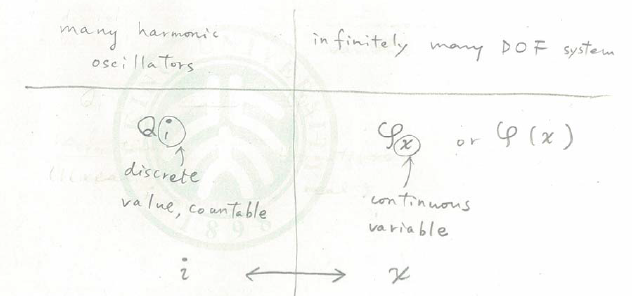
\includegraphics[width = 10cm]{1-1.png}
\end{figure}

An example of the system is a drumhead vibration. Here is a picture of drum:

\begin{figure}[h]
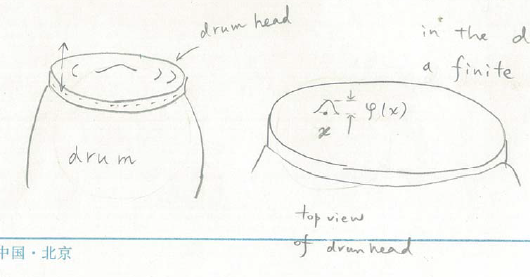
\includegraphics[width = 8cm]{1-2.png}
\end{figure}

Every spatial point in the drumhead can have a finite displacement poerpendicular to the flat drumhead. 

We can define $\varphi$ of $x$ ($\varphi(x)$) as a dispalcement at $x$ point. 

Namely, a given $\varphi$ of $x$ specifies how the drumhead is deformed from the flat drum head. 

Let us consider $\varphi$ of $x$ whose motion is described by the following Lagragian

\begin{align}
L(\varphi,\dot{\varphi}) = \frac{1}{2}\int d^2 x\dot{\varphi}(x)\dot{\varphi}(x) - \frac{1}{2}\int d^2 x \int d^2 x' K(x-x')\varphi(x)\varphi(x')\text{ with }K(x-x') = K(x'-x)
\end{align}

The corresponding equation of motion is

\begin{equation}
0 = \frac{\partial}{\partial t}\frac{\delta L}{\delta \dot{\varphi}(x)} - \frac{\delta\dot{L}}{\delta \varphi(x)} = \ddot{\varphi}(x)+\int d^2 x' K(x-x')\varphi(x')
\end{equation}

When the interaction between fields is spatially local like this

\[K(x-x') = -c^2\Delta^2\delta(x-x'), \]

the equation of motion becomes the usual wave equation

\[\nabla^2\varphi(x) - \frac{1}{c^2}\ddot{\varphi}(x) = 0 \]

\hrule

\ 

If we regard that $\varphi(x)$ is a coordinate variable for each $x$, the conjugate momentu to $\varphi$ is

\[\Pi(x) = \frac{\delta L}{\delta \dot{\varphi}(x)} = \dot{\varphi}(x) \]

The Hamiltonian is then 

\begin{align}
H = \int d^2 x \Pi(x) \dot{\varphi}(x) - L = \frac{1}{2}\int d^2 x \Pi(x)\Pi(x)+\frac{1}{2}\int d^2 x \int d^2 x' K(x-x') \varphi(x)\varphi(x')
\end{align}

To quantize the system, we suppose that $\varphi(x)$ and $\Pi(x)$ are Hermitian operators, which satisfy

\begin{align}
\begin{split}
[\varphi(x),\varphi(x')] &= [\Pi(x),\Pi(x')] = 0\\
[\varphi(x),\Pi(\varphi')] &= i\hbar\delta^2(x-x')
\end{split}
\end{align}

In such a case, it is helpful to express the field in the momentum representation, 

\[\tilde{\varphi}(k) = \int d^2 x\varphi(x)e^{-ikx} \]

\[\tilde{\Pi}(x) = \int d^2 x \Pi(x) e^{-ikx} \]

where the inverse transformation is 

\[\varphi(x) = \int\frac{d^2 k}{(2\pi)^2} \tilde{\varphi}(k)e^{ikx} \]

with

\begin{align}
\int \frac{d^2 k}{(2\pi)^2}e^{-ikx} = \delta^2(x)
\end{align}

Since $\varphi(x)$ and $\Pi(x)$ are hermitian, we have

\[\varphi^\dagger(k) = \varphi(-k) \]

\[\Pi^\dagger(k) = \Pi(-k) \]

The commutation relations are

\begin{align}
\begin{split}
[\tilde{\varphi}(k), \tilde{\varphi}(k')] &= [\tilde{\Pi}(k), \tilde{\Pi}(k')] = 0\\
[\tilde{\varphi}(k),\tilde{\Pi}(k')] &= i\hbar(2\pi)^2\delta^2(k+k')
\end{split}
\end{align}

Now let us introduce 

\[\omega^2(k) = \int d^2x K(x)e^{-ikx} \]

Since $K(x) = K(-x)$, $\omega(k)$ is real and even function in $k$. 

\[\omega^*(k) = \omega(k) = \omega(-k) \]

Let uis again assume that $\omega(k)$ are non-negative for all $k$, so that we replace this by $\omega^2(k)$. 

Rewriting the Hamiltonian in terms of these fields and functions, we obtain

\begin{align}
H = \frac{1}{2}\int\frac{d^2 k}{(2\pi)^2}\left[\tilde{\Pi}(-k)\tilde(k)+\omega^2(k)\tilde{\varphi}(-k)\tilde{\varphi}(k)\right] = \frac{1}{2}\int\frac{d^2 k}{(2\pi)^2}\left[\tilde{\Pi}^\dagger (k)\tilde(k)+\omega^2(k)\tilde{\varphi}^\dagger(k)\tilde{\varphi}(k)\right]
\end{align}

We next define annihilation and creation operators as follows, 

\begin{align}
\begin{split}
a(k) &= \frac{1}{\sqrt{2}}\left[\sqrt{\frac{\omega(k)}{\hbar}}\tilde{\varphi}(k)+\frac{i}{\sqrt{\omega(k)\hbar}}\tilde{\Pi}(k)\right]\\
a^\dagger(k) &= \frac{1}{\sqrt{2}}\left[\sqrt{\frac{\omega(k)}{\hbar}}\tilde{\varphi}(k)-\frac{i}{\sqrt{\omega(k)\hbar}}\tilde{\Pi}(k)\right]
\end{split}
\end{align}

Their commutation relations are calculated as follows, 

\[\begin{split}
[a(k),a(k')] &= \frac{1}{2\hbar}\left[\sqrt{\omega_k}\tilde{\varphi}(k)+\frac{i}{\sqrt{\omega_k}} \tilde{\Pi}(k), \sqrt{\omega_{k'}}\tilde{\varphi}(k')+\frac{i}{\sqrt{\omega_{k'}}}\tilde{\Pi}(k')\right] \\
&= \frac{1}{2\hbar}\sqrt{\frac{\omega_k}{\omega_{k'}}}i[\tilde{\varphi}(k),\tilde{\Pi}(k')] + \frac{1}{2\hbar}\sqrt{\frac{\omega_{k'}}{\omega_k}}i[\tilde{\Pi}(k),\tilde{\varphi}(k')] \\
&=(-1)(2\pi)^2\delta^2(k+k')+(2\pi)^2\delta^2(k+k')= 0 
\end{split}\]

\[[a^\dagger(k),a^\dagger(k')] = 0 \]

\begin{align}\begin{split}
[a(k),a^\dagger(k')] &= \frac{1}{2\hbar}\left[\sqrt{\omega_k}\tilde{\varphi}(k)+\frac{i}{\sqrt{\omega_k}}, \sqrt{\omega_{k'}}\tilde{\varphi}(-k') - \frac{i}{\sqrt{\omega_{k'}}}\tilde{\Pi}(-k')\right] \\
&= \frac{-i}{2\hbar}\sqrt{\frac{\omega_k}{\omega_{k'}}} [\tilde{\varphi}(k),\tilde{\Pi}(-k')] + \frac{i}{2\hbar}[\tilde{\Pi}(k),\tilde{\varphi}(-k')] \\
&= (2\pi)^2\delta^2(k-k')
\end{split}\end{align}

If we wrtie $H$ in terms of $a \& a^\dagger$, we obtain

\begin{align}
H = \frac{1}{2}\int \frac{d^2 k}{(2\pi)^2}\hbar\omega(k)[a^\dagger(k)a(k)+a(k)a^\dagger(k)] = \frac{1}{2}\int \frac{d^2 k}{(2\pi)^2}\hbar\omega(k)a^\dagger(k)a(k)+C
\end{align}

Thus, eigenstate of $H$ is given by the repeated application of $a^\dagger(k)$ onto the ground state\footnote{Regarding these energy units as particles respectively, we can think of these excited states as one-particle state, two-particle state, and so on. }

\[|k_1\rangle = a^\dagger(k_1)|0\rangle,\quad (E=\omega(k_1)) \]
\[|k_1,k_2\rangle = a^\dagger(k_1)a^\dagger(k_2)|0\rangle,\quad (E=\omega(k_1)+\omega(k_2)) \]

while the ground state satisfies

\[a(k)|0\rangle = 0,\quad\text{for}\forall k \]

To characterize these multi-particle states, let us consider the following operators, 

\begin{align}
\mathbb{P} \equiv\int\frac{d^2 k}{(2\pi)^2}\hbar{k}a^\dagger({k})a({k})
\end{align}

which satisfies

\[[\mathbb{P},a^\dagger({k})] = \hbar {k}a^\dagger(k) \]
\[[\mathbb{P},a(k)] = -\hbar ka(k) \]

so that

\[\begin{split}
\mathbb{P}|k_1,k_2,\cdots\rangle &= \mathbb{P}a^\dagger(k_1)a^\dagger(k_2)\cdots|0\rangle  = a^\dagger(k_1)(\hbar k_1+\mathbb{P})a^\dagger(k_2)\cdots|0\rangle\\
&= \hbar k_1 |k_1,k_2,\cdots\rangle + a^\dagger(k_1)\mathbb{P}a^\dagger(k_2)\cdots|0\rangle\\
&= \hbar k_1|k_1,k_2,\cdots\rangle + a^\dagger(k_1)a^\dagger(k_2)(\hbar k_2+\mathbb{P})\cdots|0\rangle\\
&=\cdots\\
&=\hbar(k_1+k_2+\cdots)|k_1,k_2,\cdots\rangle
\end{split}\]

we can also see that

\[\begin{split}
[\mathbb{P},\varphi(x)] &= \left[\mathbb{P},\int\frac{d^2k}{(2\pi)^2}\sqrt{\frac{\hbar}{2\omega(k)}}\left(a(k)e^{ik\cdot x}+a^\dagger(k)e^{-ik\cdot x}\right)\right]\\
&= \int\frac{d^2 k}{(2\pi)^2}\sqrt{\frac{\hbar}{2\omega(k)}}\left\{(-\hbar k)a(k)e^{ik\cdot x}+(\hbar k)a^\dagger(k)e^{-ik\cdot x}\right\}\\
&= i\hbar\frac{\partial}{\partial x}\left\{\int\frac{d^2 k}{(2\pi)^2}\sqrt{\frac{\hbar}{2\omega(k)}}\left(a(k)e^{ik\cdot x}+a^\dagger(k)e^{-ik\cdot x}\right)\right\}\\
&=i\hbar\frac{\partial}{\partial x}\varphi(x)
\end{split}\]

Similarly

\[[\mathbb{P},\Pi(x)] = i\hbar\cdot\frac{\partial}{\partial x}\Pi(x) \]

Using these relations, one can show that 

\[e^{a\cdot\mathbb{P}/i\hbar}\varphi(x)e^{-a\cdot\mathbb{P}/i\hbar} = \varphi(x+a) \]
\[e^{a\cdot\mathbb{P}/i\hbar}\Pi(x)e^{-a\cdot\mathbb{P}/i\hbar} = \Pi(x+a) \]

Namely, taking a derivative of r.h.s with respect to $a$, we have

\[\begin{split}
\frac{\partial}{\partial a}\left[e^{a\cdot\mathbb{P}/i\hbar}\varphi(x)e^{-a\cdot\mathbb{P}/i\hbar}\right]&=\frac{1}{i\hbar}e^{a\cdot\mathbb{P}/i\hbar}[\mathbb{P},\varphi(x)]e^{-a\cdot\mathbb{P}/i\hbar}\\
&= e^{a\cdot\mathbb{P}/i\hbar}\frac{\partial}{\partial x}\varphi(x)e^{-a\cdot\mathbb{P}/i\hbar}\\
&=\frac{\partial}{\partial x}\left\{e^{a\cdot\mathbb{P}/i\hbar}\varphi(x)e^{-a\cdot\mathbb{P}/i\hbar}\right\}
\end{split}\]

This means that

\[e^{a\cdot\mathbb{P}/i\hbar}\varphi(x)e^{-a\cdot\mathbb{P}/i\hbar} = f(x+a) \]

while $f$ should be $\phi$ when $a=0$, thus we have

\begin{align}
e^{a\cdot\mathbb{P}/i\hbar}\varphi(x)e^{-a\cdot\mathbb{P}/i\hbar} = \varphi(x+a)
\end{align}

Similar we have

\[e^{a\cdot\mathbb{P}/i\hbar}\Pi(x)e^{-a\cdot\mathbb{P}/i\hbar} = \Pi(x+a)
\]

These two relations means that $\mathbb{P}$ is a generator of the spatial translation and is therefore the momentum operator. 


\section{System of indistinguishable particles}

In the preceding sections, we consider the quantum states of an oscillator  system as multiparticle states, where each particle has an energy unit and is often called a ``phonon''. In this section, we follow a different line of reasoning. We will start with a space of states describing a single particle, which is either Bose particle or Fermi particle. We then construct the multiple-particle states based on standard methods. 

For the Bose particle case, we will arrive at a system of states and operators, that is mathematically equivalent to that found previously for a systen of oscillators. Thereby, this shows that the interpretation of oscillator states as many-phonon states is consistent with the usual description of many-particle systems with Bose statistics. 

We will develop a formalism with Fermi-Dirac statistics, for which the states do not resemble those of a harmonic-oscillator system. 

Consider first the case of distinguishable particles. 

A $n$-particle state is given by a simple product of one-particle states

\[|\psi\rangle = |\psi_1\rangle|\psi_2\rangle\cdots|\psi_n\rangle \]

You can also weite this in the coordinate representation as 

\[\psi(x_1,\cdots,x_n) = \psi_1(x_1)\psi_2(x_2)\cdots\psi_n(x_n) \]

where $x_j$ denotes the coordinate of $j$-th particle and $\langle x_j|\psi_j\rangle = \psi_j(x_j)$. 

Please notice that these $n$-particles are all distinguishable from one another. 

Namely, each particle has its own coordinate $x$, and we can distinguish $j$-th particle from $m$-th particle, because they belong to different one-particle states

\[\psi_j(x) \neq \psi_m(x),\quad \text{for }j\neq m \]

\hrule

\ 

Let us next consider indistinguishable particles. 

To make up a many-particle wavefunction for indistinguishable particles out of this, we need to make any pair of particles cannot be distinguished from each other. 

There is two-ways of doing this, one way is to ``symmetrize'' this with respect to all the possible permutations of $n$ particles:

\[\psi_1(x_1)\cdot\psi_2(x_2)\cdot\cdots\cdot\psi_n(x_n)\overset{\text{``symmetrize''}}{\longrightarrow}\frac{1}{\sqrt{n!}}\sum_P \psi_{P(1)}(x_1)\cdot\psi_{P(2)}(x_2)\cdot\cdots\cdot\psi_{P(n)}(x_n) \]

Here $P$ denotes a permutation among $n$ numbers, $\{1,2,\cdots,n\}$

\[P \equiv\left(
\begin{matrix}
1 & 2 & \cdots & n\\
P(1) & P(2) & \cdots & P(n)
\end{matrix}
\right) \]

into $\{P(1),P(2),\cdots P(n)\}$

we take the sum over all possible permutations here. 

The total number of possible permutations among $n$ distinguishable objects are given by a factorial of $n$. To normalize this many-particle wavefunction, I put $1$ over the square root of the factorial of $n$. We can see that the exchange between the $j$-th particle coordinate and the $m$-th particle coordinate does not change this many-particle wavefunction. 

\[\begin{split}
\psi(x_2,x_1,x_3,\cdots x_n) &= \frac{1}{\sqrt{n!}}\sum_P\psi_{P(1)}(x_2)\psi_{P(1)}(x_2)\psi_{P(3)}(x_3)\cdots\psi_{(P(n)}(x_n)\\
&=\frac{1}{\sqrt{n}}\sum_P\psi_{P(1)}(x_2)\psi_{P(1)}(x_2)\psi_{P(3)}(x_3)\cdots\psi_{(P(n)}(x_n)\\
\Big\{P' &= P\cdot\left(
\begin{matrix}
1 & 2 & 3 & \cdots & n\\
2 & 1 & 3 & \cdots & n
\end{matrix}\right)\Big\}\\
&=\frac{1}{\sqrt{n}}\sum_{P'}\psi_{P'(1)}(x_1)\psi_{P'(2)}(x_2)\psi_{P'(3)}(x_3)\cdots\psi_{P'(n)}(x_n)\\
&= \psi(x_1,x_2,x_3,\cdots, x_n)
\end{split}\]

Here $P'$ is a product between a permutation $P$ and the permutation which exchange $1$ and $2$, while remains other indices intact. 

This product can be regarded as a mapping from $P$ to $P'$ and this mapping is one-to-one mapping. 

Namely, a set of all possible permutations is unchanged under that mapping. 

Therefore, the right hand side is identical to the original wavefunctions. 

This argument so far holds true not only for the exchange between arbitrary pair of two particles but also for an arbitrary permutations among $n$ particles. 

\[\psi(x_{Q(1)},x_{Q(2)},\cdots,x_{Q(n)}) = \cdots=\psi(x_1,x_2,\cdots,x_n) \]

Because of this symmetrized property, $n$-particles in this wavefunction are indistinguishable from one another. 

An indistinguishable particle in a symmetrized many-particle wavefunction is called as ``boson''. 

The other way of making wavefunctions for indistinguishable particles is ``antesymmetrize'' the wavefunction for distinguishable particles. %page41

\[\Psi_F(x_1,\cdots,x_n) = \frac{1}{\sqrt{n!}}\sum_P(-1)^P\psi_{P(1)}(x_1)\cdot\psi_{P(2)}(x_2)\cdot\cdots\cdot\psi_{P(n)}(x_n) \]

Here $P$ us again in a permutation among $n$-particles, but, at this time, we have $(-1)^P$ ($(-1)$ to the power of $P$). This factor takes $+1$, if the permutation $P$ is given by a product of even-number of transpositions, where a transposition is an exchange between a pair of two particle. 

For example, 

\[
\left(\begin{matrix}
1 & 2 & 3\\ 2 & 3 & 1
\end{matrix}\right) = 
\left(\begin{matrix}
1 & 2 & 3\\ 2 & 1 & 3
\end{matrix}\right)
\cdot
\left(\begin{matrix}
1 & 2 & 3\\ 1 & 3 & 2
\end{matrix}\right)
\]

\[((1,2,3)\rightarrow(2,1,3)\rightarrow(2,3,1) \]

this permutation is given by a product of two transpositions, so that

\[(-1)^{\left(\begin{matrix}
1 & 2 & 3\\ 2 & 3 & 1
\end{matrix}\right)} = +1 \]

This factor takes $-1$, if the permutation $p$ is given by a product of odd-numbers of transpositions. 

For example, 

\[
\left(\begin{matrix}
1 & 2 & 3 & 4\\ 2 & 3 & 4 & 1
\end{matrix}\right)=
\left(\begin{matrix}
1 & 2 & 3 & 4\\ 2 & 1 & 3 & 4
\end{matrix}\right)
\cdot
\left(\begin{matrix}
1 & 2 & 3 & 4\\ 1 & 3 & 2 & 4
\end{matrix}\right)
\cdot
\left(\begin{matrix}
1 & 2 & 3 & 4\\ 1 & 2 & 4 & 3
\end{matrix}\right)
\]

this permutation is given by a product of three transpositions, so that 

\[(-1)^{\left(\begin{matrix}
1 & 2 & 3 & 4\\ 2 & 3 & 4 & 1
\end{matrix}\right)}  = -1\]

Under a permutation among $n$ particles, this many-body wavefunction is unchanged, apart from the phase factor, which is $(-1)$ to the power of $Q$. 

 \[\begin{split}
&\psi_F(x_{Q(1)},x_{Q(2)},\cdots,x_{Q(m)}) \\
&=\frac{1}{\sqrt{n!}}\sum_P(-1)^P\psi_{P(1)}(x_{Q(1)})\cdot\cdots\cdot\psi_{P(n)}(x_{Q(n)})\\
&=\frac{1}{\sqrt{n!}}\sum_P(-1)^P\psi_{P\cdot Q^{-1}(1)}(x_1)\cdot\cdots\cdot\psi_{P\cdot Q^{-1}(n)}(x_n)\\
&\quad\quad P\cdot Q^{-1}=1\\
&=(-1)^Q\frac{1}{\sqrt{n!}}\sum_{P'}(-1)^{P'}]psi_{P'(1)}(x_1)\cdot\cdots\cdot\psi_{P'(n)}(x_n)\\
&=(-1)^Q\psi_F(x_1,\cdots,x_n)
\end{split}\]

Because of this, asymmetrized property, $n$-particle in the wavefunction are essentially indistinguishable from one another. 

An indistinguishable particle in an antisymmetrized many-particle wavefunction is called as ``fermion''. 

To summarize so far, we have two way of making many-particle wavefunctions for indistinguishable particles. 

\begin{align}
|\psi\rangle &= \frac{1}{\sqrt{n!}}\sum_P\xi^P|\psi_{P(1)}\rangle|\psi_{P(2)}\rangle\cdots|\psi_{P(n)}\rangle\\
\psi(x_1,\cdots,x_n) &= \frac{1}{\sqrt{n!}}\sum_P\xi^P\psi_{P(1)}(x_1)\psi_{P(2)}(x_2)\cdot\cdots\cdot\psi_{P(n)}(x_n) = \frac{1}{\sqrt{n!}}\sum_P\xi^P\psi_1(x_{P(1)})\psi_2(x_{P(2)})\cdot\cdots\cdot\psi_n(x_{P(n)}) \end{align}

where $\xi = \pm1$ for boson and fermion. 

We will write this as $|\psi_1,\psi_2,\psi_n,\cdots\psi_n\rangle$. 

Let us show an example:

Suppose that $|\psi_1\rangle$ and $|\psi_2\rangle$ are two orthonormal single-particle states. 

For bose particles, we can make three many-particle wavefunctions out of them. One is this, and the other is

\[\begin{split}
|\Psi_a\rangle &= \frac{1}{\sqrt{2!}}(|\psi_1\rangle|\psi_2\rangle + |\psi_2\rangle|\psi_1\rangle)\\
|\Psi_b\rangle &= \frac{1}{\sqrt{2!}}(|\psi_1\rangle|\psi_1\rangle + |\psi_1\rangle|\psi_1\rangle) = \sqrt{2}|\psi_1\rangle|\psi_1\rangle\\
|\Psi_c\rangle &= \frac{1}{\sqrt{2!}}(\psi_2\rangle|\psi_2\rangle + \psi_2\rangle|\psi_2\rangle) = \sqrt{2}\psi_2\rangle|\psi_2\rangle
\end{split} \]

For fermi particles, we can make only one many-particle wavefunctions, 

\[\begin{split}
|\Psi_a\rangle &= \frac{1}{\sqrt{2!}}(|\psi_1\rangle|\psi_2\rangle - |\psi_2\rangle|\psi_1\rangle) \\
|\Psi_b\rangle &= \frac{1}{\sqrt{2!}}(|\psi_1\rangle|\psi_1\rangle - |\psi_1\rangle|\psi_1\rangle) = 0 \\
|\Psi_b\rangle &= \frac{1}{\sqrt{2!}}(|\psi_2\rangle|\psi_2\rangle - |\psi_2\rangle|\psi_2\rangle) = 0 
\end{split}\] 

This two dictates that, due to the antisymmetric character, two fermi particles cannot occupy the same state. 

The inner product of two of these $n$-particle states are given by a determinent or permanent of a $n\times n$ matrix, which is composed by the inner products of single particle states. 

\begin{align}
\langle\varphi_1,\cdots,\varphi_n|\psi_1,\cdots,\psi_n\rangle = \begin{vmatrix}
\langle \varphi_1|\psi_1\rangle & \langle \varphi_1|\psi_2\rangle & \cdots & \langle \varphi_1|\psi_n\rangle\\
\langle \varphi_2|\psi_1\rangle & \langle \varphi_2|\psi_2\rangle & \cdots & \langle \varphi_2|\psi_n\rangle\\
\cdots & \cdots & \cdots & \cdots\\
\langle \varphi_n|\psi_1\rangle & \langle \varphi_n|\psi_2\rangle & \cdots & \langle \varphi_n|\psi_n\rangle
\end{vmatrix}
\end{align}

where 

\[\langle\varphi_j|\psi_m\rangle = \int d^d {\bf x}\varphi_j^*({\bf x})\psi_m({\bf x}) \]

and

\[|{\bf A}|_{\xi} = \sum_{P}\xi^P {\bf A}_{1P(1)}\cdots{\bf A}_{nP(n)} \]

with $n\times n$ matrix ${\bf A} = ({\bf A}_{ij})$

Namely, $|{\bf A}|$ is a determinant of ${\bf A}$ while ${\bf A}_+$ is a permanent of ${\bf A}$. 

\hrule

\ 

One can prove this straightforwardly, 

\[\begin{split}
&\langle\varphi_1,\cdots,\varphi_n|\psi_1,\cdots,\psi_n\rangle =\frac{1}{n!}\sum_P\sum_Q\xi^P\xi^Q\langle\varphi_{P(1)}|\psi_{Q(1)}\rangle\cdots\langle\varphi_{P(n)}|\psi_{Q(n)}\rangle \\
& = \frac{1}{n!}\sum_{P}\sum_{Q}\xi^P\xi^Q\langle\varphi_1|\psi_{QP^{-1}(1)}\rangle\cdots\langle\varphi_n|\psi_{QP^{-1}(n)}\rangle\\
&\quad (\xi^P)^{-1} = \xi^P,\quad R\equiv Q\cdot P^{-1}\\
&= \frac{1}{n!} \sum_P\sum_Q\xi^R\langle\varphi_1|\psi_{R(1)}\rangle\cdots\langle\varphi_n|\psi_{R(n)}\rangle
\end{split}\]

\[\sum_P\sum_Q = \sum_P\sum_{QP^{-1}}=\sum_P\sum_R \]

Now that the summation is free from $P$, the summation over $P$ just gives us a factor $n!$, which set off this. 

Thus, we have

\[\langle\varphi_1,\cdots,\varphi_n|\psi_1,\cdots,\psi_n\rangle = \sum_R\xi^R\langle\varphi_1|\psi_{R(1)}\rangle\cdots\langle\varphi_n|\psi_{R(n)}\rangle = |(\langle\varphi_i|\psi_j\rangle)|_\xi \]

Suppose that $\{|1\rangle,|2\rangle,\cdots\}$ is a complete orthonormal set of single-particle states:

\[\alpha|\beta\rangle = \delta_{\alpha\beta},\quad\sum_{\alpha}|\alpha\rangle\langle\alpha| = 1 \]

A complete set of $n$-particle states consists of $|\alpha_1,\alpha_2,\cdots,\alpha_n\rangle$ where $\alpha_1\le\cdots\le\alpha_n$ in the Bose case, and $\alpha_1<\alpha_2<\cdots<\alpha_n$ in the fermion case. 

These states are orthogonal to one another, but not always normalized in the Bose case. 

Using this, one can show that a complete orthonormal set of $n$-particle states consist of

\begin{align}\begin{cases}
\displaystyle\frac{|\alpha_1,\alpha_2,\cdots,\alpha_n\rangle}{\sqrt{n_1!n_2!\cdots}} \quad (\alpha_1\le\cdots\le\alpha_n) \ \text{for boson}\\
\ \\
|\alpha_1,\alpha_2,\cdots\alpha_n\rangle \quad (\alpha_1<\alpha_2<\cdots<\alpha_n)\ \text(for fermion)
\end{cases}\end{align}

where $n_j$ denotes the number of times that $j$ occurs in the sequence of $\alpha_1,\cdots,\alpha_n$. 

For either boson case or fermion case, the completeness relation in the $n$-particles space can be weitten in the following simple form. 

\begin{align}
\frac{1}{n!}\sum_{\alpha_1}\cdots\sum_{\alpha_n}|\alpha_1,\cdots,\alpha_n\rangle\langle\alpha)_1,\cdots,\alpha_n| = 1
\end{align}

where the sum of each $\alpha_j$ is taken over all single-particle states. 

The duplication of $n$-particle states are set off by the $1/n!$ (one over the factorial of $n$) and the normalization. 

To see that this equality holds true for both boson and fermion cases, let us apply the left side to a $n$-particle state $|\beta_1,\cdots,\beta_n\rangle$ where $|\beta_j\rangle$ is from $\{|1\rangle,|2\rangle,\cdots,\}$ the single-particle states considered. \\

{\Huge 1. }When all these $\beta_j$ are distict from one another, 

\[\begin{split}
&\frac{1}{n!}\sum_{\alpha_1}\cdots\sum_{\alpha_n}|\alpha_1,\cdots,\alpha_n\rangle\langle\alpha_1,\cdots,\alpha_n|\beta_1,\cdots,\beta_n\rangle\\
&=\frac{1}{n!}\sum_P|P(\beta_1),P(\beta_2),\cdots,P(\beta_n)\rangle\langle P(\beta_1),P(\beta_2),\cdots,P(\beta_n)|\beta_1,\cdots,\beta_n\rangle\\
&=\frac{1}{n!}\sum_P\xi^P|P(\beta_1),P(\beta_2),\cdots,P(\beta_n)\rangle\\
&=\frac{1}{n!}\sum_P|\beta_1,\cdots,\beta_n\rangle = |\beta_1,\cdots,\beta_n\rangle
\end{split}\]

{\Huge 2. }When some of these $\beta_j$ are identical, which can be the case with bose particles, 

\[\begin{split}
&\frac{1}{n!}\sum_{\alpha_1}\cdots\sum_{\alpha_n}|\alpha_1,\cdots,\alpha_n\rangle\langle\alpha_1,\cdots,\alpha_n|\beta_1,\cdots,\beta_n\rangle \\
&= \frac{1}{n!}{\color{red}{\tilde{\sum_P}}}|P(\beta_1),P(\beta_2),\cdots,P(\beta_n)\rangle\langle P(\beta_1),P(\beta_2),\cdots,P(\beta_n)|\beta_1,\cdots,\beta_n\rangle \end{split}\]

Here the {\color{red}{summation}} of $P$ is taken over all possible permutations of $n$-objects with duplications being excluded. 

Namely, $\tilde{\sum_P}$ does count the following permutations separately. It counts one of them once and doesn't count the others. 

\[
\begin{split}
&P_1(\beta_j) = P_2(\beta_j) = P_3(\beta_j)=\cdots=P_m(\beta_j), \text{ for }\forall j = 1,\cdots,n\\ 
&=\frac{1}{n!}\tilde{\sum_P}|P(\beta_1),\cdots,P(\beta_n)\rangle\times(n_1!\cdot n_2!\cdots)
\end{split}\]

where $n_j$ denotes the number of times that ``$j$'' occurs in the sequence of $\beta_1,\cdots,\beta_n$. 

Now that 

\[|P(\beta_1),\cdots,P(\beta_n)\rangle = |\beta_1,\cdots,\beta_n\rangle \]

and

\[\tilde{\sum_P} = \frac{n!}{n_1!\cdot n_2!\cdot\cdots} \]

the right hand side is

\[=|\beta_1,\beta_2,\cdots,\beta_n\rangle \]

\ 

These two ({\Huge 1, 2}) prove that this completeness relation holds true for both boson case and fermion case. \\

\hrule

\ 

In actual physical process, the number of particles is not constant in time. Particles can be constructed and destroyed. To describe such process, we need a Hilbert space that contains states of varying number of particles. To get such a space, we simply combine all the $n$-particle spaces into one big space that we call the ``multiparticle space''. 

A general state in the multiparticle space is of the from of 

\[|\psi\rangle = |\psi^{(0)}\rangle + |\psi^{(1)}\rangle + |\psi^{(2)}\rangle + \cdots \]

where $|\psi^{(n)}\rangle$ is an $n$-particle state and $|\psi^{(0)}\rangle$ is just a vacuum state

\[|\psi^{(0)}\rangle = |var\rangle \]

States of differemt numbers of particles are defined to be orthogonal to each other, so that

\[\langle\varphi|\psi\rangle = \langle\varphi^{(0)}|\psi^{(0)}\rangle + \langle\varphi^{(1)}|\psi^{(1)}\rangle  \]

where

\[|\varphi\rangle = |\varphi^{(0)}\rangle + |\varphi^{(1)}\rangle + \cdots \]

The completeness relation in the multiparticle is given as follows, 

\begin{align}
\sum_{n=1}^{\infty}\frac{1}{n!}\sum_{\alpha_1}\cdots\sum_{\alpha_n}|\alpha_1,\cdots,\alpha_n\rangle\langle \alpha_1,\cdots,\alpha_n| = 1
\end{align}



\section{Creation operator \& destruction operator}

So far, we have constructed a complete orthonormal set of states in the multiparticle space. With these constructions in hand, we are now ready to define creation and destruction operators. These operators change the number of particles, so that they connect states of different numbers of particles. We will see that allthe physical operators are expressed in terms of creation and destruction operators. 

Let $|\varphi\rangle$ be any one-particle state. We define $a^\dagger$ of $\varphi$ to be that linear operator which satisfies this, for any n-particle states $|\psi_1, \cdots,\psi_n\rangle$. 

\begin{align}
a^\dagger{\varphi}|\psi_1,\cdots,\psi_n\rangle = |\varphi,\psi_1,\cdots,\psi_n\rangle \tag{e}\\
\quad\text{for any}|\psi_1,\cdots,\psi_n\rangle \label{Eqs1.6.1}
\end{align}

For $n=0$, this simply means that

\[a^\dagger(\varphi)|vac\rangle = |\varphi\rangle \]

We call $a^\dagger(\varphi)$ as the creation operator for the state $|\varphi\rangle$, and its hermitian conjugate $a(\varphi)$ as the destruction or annihilation operator. 

A destruction operator converts an $n$-particle states into a $(n-1)$-particle states. 

To find the effect of $a(\varphi)$ on an $n$-particle state $|\psi_1,\psi_2,\cdots,\psi_n\rangle$, we multiply on the left by an arbitrary $(n-1)$-particle state, which is this

\[\begin{split}
&\langle x_1,\cdots,x_{n-1}|a(\varphi)|\psi_1,\cdots,\psi_n\rangle \\
&= (\langle \psi_1,\cdots,\psi_n|a^\dagger(\varphi)|x_1,\cdots,x_{n-1}\rangle)^*\\
&= (\langle \psi_1,\cdots,\psi_n|\varphi,x_1,\cdots,x_{n-1}\rangle)^*\\
&= 
\begin{vmatrix}
\langle\psi_1|\phi\rangle & \langle\psi_1|x_1\rangle & \cdots & \langle\psi_1|x_{n-1}\rangle\\
\langle\psi_2|\phi\rangle & \langle\psi_2|x_1\rangle & \cdots & \langle\psi_2|x_{n-1}\rangle\\
\cdots & \cdots & \cdots & \cdots \\
\langle\psi_n|\phi\rangle & \langle\psi_n|x_1\rangle & \cdots & \langle\psi_n|x_{n-1}\rangle
\end{vmatrix}_{\xi}^*\\
&= \left\{\sum_{k=1}^n \xi^{k-1}\langle\psi_k|\varphi\rangle
\begin{vmatrix}
 \langle\psi_1|x_1\rangle & \cdots & \langle\psi_1|x_{n-1}\rangle\\
 \langle\psi_2|x_1\rangle & \cdots & \langle\psi_2|x_{n-1}\rangle\\
 \cdots & \cdots & \cdots \\
 \langle\psi_n|x_1\rangle & \cdots & \langle\psi_n|x_{n-1}\rangle
\end{vmatrix}_{\xi} \right\}^*\\
&= \sum_{k=1}^n \xi^{k-1}\langle\varphi|\psi_k\rangle\langle x_1,\cdots,x_{n-1}|\psi_1,\cdots,\psi_{k-1},\psi_{k+1},\cdots,\psi_n\rangle
\end{split}\]

Since this relation holds true for any arbitrary $x_1$ and so on, we finally have

\begin{align}\label{Eqs1.6.2}a(\varphi)|\psi_1,\cdots,\psi_n\rangle = \sum_{k=1}^n \xi^{k-1}\langle \varphi|\psi_k\rangle |\psi_1,\cdots,\psi_{k-1},\psi_{k+1},\cdots,\psi_n\rangle \end{align}


We can derive 

\[a^\dagger(\varphi_1)a^\dagger(\varphi_2) = \xi a^\dagger(\varphi_2)a^\dagger(\varphi) \]

Namely, the following relations holds true for arbitrary $\psi_1,\cdots,\psi_n$

\[a^\dagger(\varphi_1)a^\dagger(\varphi_2)|\psi_1,\cdots,\psi_n\rangle = \xi a^\dagger(\varphi_2)a^\dagger(\varphi) |\psi_1,\cdots,\psi_n\rangle\]

This leads to the commutation relations for boson and fermion. 

\begin{align}
[a^\dagger(\varphi_1),a^\dagger(\varphi_2)]_{-\xi} = 0
\end{align}

where

\[[A,B]_{-\xi} = AB - \xi BA = \begin{cases}AB-BA\ \text{boson}\\ \ \\ AB+BA \ \text{fermion}\end{cases}\]

Taking the hermite conjugate of this, we have

\begin{align}
[a(\varphi_1),a(\varphi_2)]_{-\xi} = 0
\end{align}

\hrule

\ 

To find the commutation relations between the creation operator and destruction operator, we first calculate 

\[\begin{split}
&a(\varphi_1)a^\dagger(\varphi_2)|\psi_1,\cdots,\psi_n\rangle \\
&=a(\varphi_1)|\varphi_2,\psi_1,\cdots,\psi_n\rangle\\
&= \langle\varphi_1|\varphi_2\rangle|\psi_1,\cdots,\psi_n\rangle + \sum_{k=1}^n\xi^k\langle\varphi_1|\psi_k\rangle|\varphi_2,\psi_1,\cdots,\psi_{k-1},\psi_{k+1},\cdots,\psi_n\rangle
\end{split}\]

and

\[\begin{split}
&a^\dagger(\varphi_2)a(\varphi_1)|\psi_1,\cdots,\psi_n\rangle \\
&= \sum_{k=1}^n\xi^{k-1}\langle \varphi_1|\psi_k\rangle a^\dagger(\varphi_2)|\psi_k\rangle|\varphi_2,\psi_1,\cdots,\psi_{k-1},\psi_{k+1},\cdots,\psi_n\rangle\\
&= \sum_{k=1}^n\xi^{k-1}\langle \varphi_1|\psi_k\rangle |\varphi_2,\psi_k\rangle|\varphi_2,\psi_1,\cdots,\psi_{k-1},\psi_{k+1},\cdots,\psi_n\rangle\\
\end{split}\]

Multiply this by $\xi$ and substract it from the former one, we see that

\[[a(\varphi_1)a^\dagger(\varphi_2) - \xi a^\dagger(\varphi_2)a(\varphi_2)]|\psi_1,\cdots,\psi_n\rangle = \langle \varphi_1|\varphi_2\rangle |\psi_1,\cdots,\psi_n\rangle \]

Equivalently, we have

\begin{align}\label{eqs1.6.5}
[a(\varphi_1),a^\dagger(\varphi_2)] _{-\xi} = \langle\varphi_1|\varphi_2\rangle
\end{align}

These three relations are the fundamental ``commutation relations'' for creation \& destruction operators. When these operators are introduced in terms of an orthonormal basis, this relation becomes

\begin{align}
[a(\alpha),a^\dagger(\beta)]_{-\xi} = \langle\alpha|\beta\rangle = \delta_{\alpha\beta}
\end{align}

Where one-particle states $|\alpha\rangle$ and $|\beta\rangle$ are from a complete orthonormal set of one-particle states, $\{|1\rangle,|2\rangle,\cdots\}$

Let us next compare these commutation relations with raising and lowering operators for linear harmonic osciallators. 

For boson case, we further define an orthonormal basis for the multiparticle space as 

\begin{align}|n_1,n_2,\cdots\rangle = \frac{|\overset{n_1}{1,\cdots,1},\overset{n_2}{2,\cdots,2},\cdots\rangle}{\sqrt{n_1! n_2!,\cdots}} \end{align}

Where we use $\{|1\rangle,|2\rangle,\cdots\}$ as a complete orthonormal set of one-particle states and $n_{\alpha}$ is the number of times $\alpha$ appear in the ket state in the right hand side. In terms of this orthornormal basis, eqs \eqref{Eqs1.6.1}, \eqref{Eqs1.6.2} reduce to the followings:

\begin{align}
a^\dagger(\alpha)|n_1,n_2,\cdots,n_{\alpha},\cdots\rangle = \sqrt{n_\alpha+1}|n_1,n_2,\cdots,n_{\alpha}+1,\cdots\rangle\\
a(\alpha)|n_1,n_2,\cdots,n_{\alpha},\cdots\rangle = \sqrt{n_\alpha}|n_1,n_2,\cdots,n_{\alpha}-1,\cdots\rangle
\end{align}

while the commutation relations are 

\begin{equation}
\begin{split}
[a(\alpha),a(\beta)] &= [a^\dagger(\alpha),a^\dagger(\beta)] = 0\\
[a(\alpha),a^\dagger(\beta)] &= \delta_{\alpha\beta}
\end{split}
\end{equation}

These three equations are identical to eqs \eqref{Eqs1.3.2}, \eqref{Eqs1.3.3}, \eqref{Eqs1.3.4}

This means that creation \& destruction operators for a system of Bose particles looks exactly like those for a system of linear harmonic oscillators. 

For fermions case, we have

\begin{align}
\begin{split}
a_\alpha^\dagger|\alpha_1,\cdots,\alpha_n\rangle &= |\alpha,\alpha_1,\cdots,\alpha_n\rangle\\
a_\alpha|\alpha_1,\cdots,\alpha_n\rangle &= \sum_{k=1}^n(-1)^{k-1}\delta_{\alpha\alpha_k}|\alpha_1,\cdots,\alpha_{k-1},\alpha_{k+1},\cdots,\alpha_n\rangle
\end{split}
\end{align}

\begin{align}
\begin{cases}
[a_\alpha,a_\beta]_+ = [a_\alpha^\dagger,a_\beta^\dagger] = 0\\
[a_\alpha,a_\beta^\dagger]_+ = \delta_{\alpha\beta}
\end{cases}
\end{align}

Contrary to the boson case, there is no a priori reason for  postulating these anticommutation relations. These relations can be derived only from the antisymmetrization postulate for fermions. 

Let us put some remarks on these general commutation relations. 

One advantage of deriving them in such a general form is that we are not tied down to a particular basis of one-particle states. Suppose we use a basis of momentum eigenstates, $|\bf p\rangle$ with $\langle{\bf p}|{\bf p'}\rangle = (2\pi)^3\delta^3({\bf p}-{\bf p'})$. Then we have

\begin{align}
\begin{split}
[a({\bf p}),a^\dagger({\bf p'})]_{-\xi}&=(2\pi)^3\delta^3({\bf p}-{\bf p'})\\
[a({\bf p}), a({\bf p'})]_{-\xi} &= [a^\dagger({\bf p}),a^\dagger({\bf p'})]_{-\xi} = 0
\end{split}
\end{align}

A complete orthogonal sets of states in the multiparticle space can be constructed from the vacuum state 

\[|{\bf p_1},{\bf p_2},\cdots,{\bf p_n}\rangle = a^\dagger({\bf p_1})\cdots a^\dagger({\bf p_n})|vac\rangle \]

If we use a basis of position eigenstates $|\bf{x}\rangle$ with $\langle {\bf x}|{\bf x'}\rangle = \delta^3({\bf x} - {\bf x'})$

\begin{align}
[a({\bf x}),a^\dagger({\bf x'})] = \delta^3({\bf x} - {\bf x'})
\end{align}

\[|{\bf x}_1,\cdots,{\bf x}_n\rangle = a^\dagger({\bf x}_1)\cdots a^\dagger({\bf x}_n)|vac\rangle \]

When we change a basis for one-particle states, the creation operators ``transform'' like ket state, while the destruction operators ``transform'' like bra state. 

\[|{\bf x}\rangle = \alpha|\psi\rangle + \beta|\varphi\rangle \]
\[\langle{\bf x}| = \langle\psi|\alpha^* + \langle\varphi|\beta^* \]

\[\begin{cases}
a^\dagger({\bf x}) &= \alpha a^\dagger(\psi)+\beta a^\dagger(\varphi)\\
a({\bf x}) &= \alpha^* a(\psi) + \beta^* a(\varphi)
\end{cases}\]

Notice: for $\forall \psi_1,\cdots$

\[a^\dagger({\bf x})|\psi_1,\cdots\rangle = |\alpha\psi+\beta\varphi,\psi\cdots\rangle = \alpha|\psi,\psi_1,\cdots\rangle + \beta|\varphi,\psi_1,\cdots\rangle = \alpha a^\dagger(\psi)|\psi,\cdots\rangle + \beta a^\dagger(\varphi)|\psi_1\cdots\rangle \]

Now if we change from position representation to momentum representation:

\[\begin{split}
|{\bf p}\rangle = \int d^3{\bf x} |{\bf x}\rangle\langle{\bf x}|{\bf p}\rangle = \int d^3{\bf x}|{\bf x}\rangle e^{i{\bf p}\cdot{\bf x}}\\
|{\bf x}\rangle = \int d^3{\bf p} |{\bf p}\rangle\langle{\bf p}|{\bf x}\rangle = \int d^3{\bf p}|{\bf p}\rangle e^{-i{\bf p}\cdot{\bf x}}
\end{split}\]

The respective creation operators are related to each other as 

\begin{align}
\begin{split}
a^\dagger({\bf p}) = \int d^3{\bf x} a^\dagger({\bf x}) e^{i{\bf p}\cdot{\bf x}}\\
a^\dagger({\bf x}) = \int d^3{\bf p} a^\dagger({\bf p}) e^{-i{\bf p}\cdot{\bf x}}
\end{split}
\end{align}

\section{Hamiltonian and other operators of creation and destruction operators}

So far, we developed a method of describing systems containing many Bose or Fermi particles, and define creation \& destruction operators. In the following, we will see that these operators have other use than merely creating or annihilating particles. 

Suppose that $A^{(1)}$ is an operator that acts on one-particle states

\begin{align}
\begin{split}
\hat{A}^{(1)}({\bf x},{\bf p})|\psi\rangle = |\psi'\rangle \\
\text{or}\\
\hat{A}^{(1)}\left({\bf x},-i\frac{\partial}{\partial {\bf x}}\right)\psi({\bf x}) = \psi'({\bf x})
\end{split}
\end{align}

In many-particle systems, we often want to deal with an operator that represents the ``sum of $A^{(1)}$ over all of the particles. ''

\begin{align}
\hat{A}\overset{def}{\equiv}\sum_j\hat{A}^{(1)}({\bf x}_j,{\bf p}_j)
\end{align}

Thus, we want to represent $\hat{A}$ in terms of the creation and destruction operators. 

To do this, we fiesr describe this, we first describe this single-particle operator $\hat{A}^{(1)}$ in terms of a complete orthonormal set of one-particle states: $\{|\alpha\rangle\} = \{|1\rangle,|2\rangle,\cdots\}$

\begin{align}
\hat{A}^{(1)}({\bf \hat{x}, \hat{p}}) \equiv \sum_{\alpha,\beta}|\alpha\rangle\langle\alpha| \hat{A}^{(1)}|\beta\rangle\langle\beta| = \alpha_{\alpha,\beta}\hat{A}^{(1)}_{\alpha\beta}|\alpha\rangle\langle\beta
\end{align}

with

\begin{align}
\begin{split}
\hat{A}^{(1)}_{\alpha\beta} &\equiv\langle\alpha|\hat{A}^{(1)}({\bf \hat{x},\hat{p}})|\beta\rangle \\
&=\int d{\bf x} \langle\alpha|{\bf x}\rangle\hat{A}^{(1)}({\bf x}, -i\frac{\partial}{\partial{\bf x}})\langle{\bf x}|\beta\rangle
\end{split}
\end{align}

With this, let us apply $\hat{A}$ to an arbitray state in the multiparticle space

\[\begin{split}
&\hat{A}\langle x_1,\cdots,x_n|\psi_1,\cdots,\psi_n\rangle \\
&=\hat{A}\frac{1}{\sqrt{n!}}\sum_P\xi^P\langle x_{P(1)}|\psi_1\rangle\cdot\langle x_{P(2)}|\psi_2\rangle\cdot\cdots\cdot\langle x_{P(n)}|\psi_n\rangle\\
&=\frac{1}{\sqrt{n!}}\sum_P\xi^P\{\hat{A}\langle x_{P(1)}|\psi_1\rangle\}\cdot\langle x_{P(2)}|\psi_2\rangle\cdot\cdots\cdot\langle x_{P(n)}|\psi_n\rangle \\
&\quad + \frac{1}{\sqrt{n!}}\sum_P\xi^P\langle x_{P(1)}|\psi_1\rangle\cdot\{\hat{A}\langle x_{P(2)}|\psi_2\rangle\}\cdot\cdots\cdot\langle x_{P(n)}|\psi_n\rangle + \cdots
\end{split}\]

Now that we can calculate each term in the single-particle space

\[\begin{split}
&\hat{A}_1(x_{P(j)},-i\frac{\partial}{\partial x_{P(j)}}\langle x_{P(j)}|\psi_j\rangle = \sum_{\alpha,\beta}\langle x_{P(j)}|\alpha\rangle A^{(1)}_{\alpha\beta}\langle\beta|\psi_j\rangle \\
&= \sum_{\alpha,\beta}A^{(1)}_{\alpha\beta}\cdot\frac{1}{\sqrt{n1}}\sum_P\xi^P \times \\
&\Big\{\langle x_{P(1)}|\alpha\rangle\langle\beta|\psi_1\rangle\langle x_{P(2)}|\psi_2\rangle\cdot\cdots\cdot\langle x_{P(n)}|\psi_n\rangle\\
&\quad +\langle x_{P(1)}|\psi_1\rangle\langle x_{P(2)}|\alpha\rangle\beta|\psi_2\rangle\cdot\cdots\cdot\langle x_{P(n)}|\psi_n\rangle + \cdots\Big\}\\
&=\sum_{\alpha,\beta}A_{\alpha\beta}^{(1)}\times\\
&\Big\{\langle\beta|\psi_1\rangle\langle x_1,\cdots,x_n|\alpha,\psi_2,\cdots,\psi_n\rangle\\
&\quad +\langle\beta|\psi_2\rangle\langle x_1,\cdots,x_n|\psi_1,\alpha,\cdots,\psi_n\rangle + \cdots\Big\}
\end{split}\]

Now that

\[\begin{split}
&a^\dagger(\alpha) a(\beta)|\psi_1,\psi_2,\cdots,\psi_n\rangle \\
&= \sum_{k=1}^n\xi^{k-1}\langle \beta|\psi_k\rangle|\alpha,\psi_1,\cdots,\psi_{k-1},\psi_{k+1},\cdots,\psi_n\rangle\\
&=\sum_{k=1}^n\langle\beta|\psi_k\rangle|\psi_1,\psi_2,\cdots,\psi_{k-1},\alpha,\psi_{k+1},\cdots,\psi_n\rangle
\end{split}\]

Thus

\[=\sum_{\alpha,\beta}A_{\alpha\beta}^{(1)}\langle x_1,\cdots,x_n|a^\dagger(\alpha)a(\beta)|\psi_1,\cdots,\psi_n\rangle \]

To summarize, we have

\begin{align}
\hat{A}\langle x_1,\cdots,x_n|\psi_1,\cdots,\psi_n\rangle = \langle x_1,\cdots,x_n|\sum_{\alpha,\beta}A_{\alpha\beta}^{(1)}a^\dagger(\alpha)a(\beta)|\psi_1,\cdots,\psi_n\rangle
\end{align}

From this, we can write the sum of the single-particle operator over all particles in terms of creation \& destruction operators as 

\[\hat{A} = \sum_j\hat{A}^{(1)}({\bf x}_j,-i\frac{\partial}{\partial {\bf x}_j}) \]

\begin{align}\label{eqs1.7.6}
\rightarrow \hat{A} = \sum_{\alpha,\beta} A^{(1)}_{\alpha\beta}a^\dagger(\alpha)a(\beta)
\end{align}

where

\[A^{(1)}_{\alpha\beta} = \int d{\bf x} \langle\alpha|{\bf x}\rangle\hat{A}^{(1)}({\bf x}, -i\frac{\partial}{\partial{\bf x}})\langle{\bf x}|\beta\rangle\]

\hrule
\smallskip
\hrule


\ 

As a first example, we consider $A^{(1)} = 1$ (identity operator in the single-particle space) the sum of this over all particles can be expressed by the creation \& destruction operators as 

\[\hat{A} = \sum_j \hat{1}\]
\begin{align}
\rightarrow\hat{A} = \sum_{\alpha,\beta}\langle\alpha|\hat{1}|\beta\rangle a^\dagger(\alpha)a(\beta) = \sum_{\alpha,\beta}\delta_{\alpha\beta}a^\dagger(\alpha)a(\beta) = \sum_\alpha a^\dagger(\alpha)a(\alpha)
\end{align}

Using other basis, we can rewrite this into

\begin{align}
\begin{split} 
&=\int d^3{\bf x}\int d^3{\bf x'}\underset{\delta^3(\bf x-x')}{\langle\bf x|x'\rangle}a^\dagger({\bf x})a({\bf x})\\
&=\int d^3{\bf x}a^\dagger{\bf x}a({\bf x'})
\end{split}\\
\begin{split}
&=\int \frac{d^3{\bf p}}{(2\pi)^3}\int \frac{d^3\bf p'}{(2\pi)^3}\underset{(2\pi)^3\delta^3(\bf p - p')}{\langle\bf p|p'\rangle}a^\dagger({\bf p})a({\bf p'})\\
&=\int \frac{d^3\bf p}a^\dagger({\bf p})a({\bf p})
\end{split}
\end{align}

Next consider the momentum operator in the single-particle space

\[{\bf P}^{(1)} = \int \frac{d^3\bf p}{\bf p|p\rangle\langle p|} = \int d^3{\bf x}|{\bf x}\rangle(-i)\frac{\partial}{\partial{\bf x}}\langle\bf x|  \]

We have for the total momentum

\begin{align}
\begin{split}
{\bf P} &=  \int \frac{d^3\bf p}{\bf p}a^\dagger({\bf p})a({\bf p})\\& = \int d^3{\bf x}a^\dagger({\bf x})\frac{\partial}{i\partial\bf x}a(\bf x)
\end{split}
\end{align}

Finally, consider the Hamiltonian for a single particle:

\[H^{(1)}=\frac{\bf p^2}{2m}+V(\bf x) \]

In the coordinate representation, this is given by

\[\langle{\bf x}|H^{(1)}|{\bf x'}\rangle = -\frac{1}{2m}\nabla_{\bf x}^2\delta({\bf x-x'})+V({\bf x})\delta(\bf x - x') \]

Thus, the sum of this over all particles are given by the creation \& destruction operators in this way

\begin{align}
\begin{split}
H &= \int d^3{\bf x}d^3{\bf x'}a^\dagger({\bf x})\left[-\frac{\nabla_{\bf x}^2}{2m}\delta({\bf x-x'})+V({\bf x})\delta({\bf x - x'})\right]a(\bf x')\\
&=\int d^3{\bf x}a^\dagger({\bf x})\left[-\frac{\nabla_{\bf x}^2}{2m}+V({\bf x})\right]a(\bf x)
\end{split}
\end{align}

In the momentum representation, it takes the form of

\begin{align}
=\int\frac{d^3\bf p}{(2\pi)^3} \frac{\bf p^2}{2m}a^\dagger({\bf p})a({\bf p})+\int\frac{d^3\bf p}{(2\pi)^3}\int\frac{d^3\bf q}{(2\pi)^3}\tilde{V}({\bf q})a^\dagger({\bf p+q})a({\bf p})
\end{align}

where 

\[\tilde{V}({\bf q}) \equiv\int d^3{\bf x} V({\bf x})e^{-i\bf q\cdot x} \]

If we use a basis of eigenstate of $H^{(1)}$

\[\langle\alpha|H^{(1)}|\beta\rangle = E_\alpha\delta_{\alpha\beta} \]

it takes the form of

\begin{align}
=\sum_\alpha E_\alpha a^\dagger(\alpha)a(\alpha)
\end{align}

The density of particles per unit volume at the point $\bf x$ is defined as 

\[\hat{\rho}({\bf x}) = \sum_j\delta({\bf x - x}_j),\quad j\text{, the particle index} \]

In terms of the creation \& annihilation operators in the coordinate representation, 

\[\hat{\rho}({\bf x}) = \int d^3{\bf y}\int d^3{\bf y'}a^\dagger({\bf y})a({\bf y'})\times\langle{\bf y}|\hat{\rho}(\bf x)|y'\rangle \]

where

\begin{align}
\begin{split}
&\langle {\bf y}|\hat{\rho}({\bf x})|{\bf y'}\rangle\\
&=\int d^3{\bf y''}\delta^3({\bf y - y''})\delta^3){\bf y'-y''})'delta(\bf x - y'')\\
&=\delta^3({\bf y - x})\delta^3(\bf y' - x)\\
&=a^\dagger({\bf x})a(\bf x)
\end{split}
\end{align}

In fact, total number of particles is defined as the integral of this over ${\bf x}_j$

\begin{align}\label{eqs1.7.15}
\hat{N}=\int d^3{\bf x}\hat{\rho}({\bf x}) = \int d^3{\bf x}a^\dagger({\bf x})a(\bf x)
\end{align}

which is consistant with the previous expression for $\hat{N}$

In terms of this density operator, the $2$nd term in equation can be given as the integral of the potential energy weighted by the density

\[V = \int d^3{\bf x}V({\bf x})\hat{\rho}(\bf x) \]

So far, we have described a system of independent particles, where two or more particles are not influencing one another. 

In the following, we will develop how interactions between particles are described in the $2$nd quantization language. 

\begin{wrapfigure}{l}{6cm}%????????
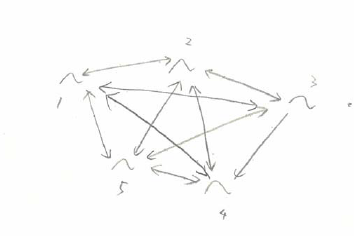
\includegraphics[width = 4.5cm]{1-3.png}
\end{wrapfigure}

As the simplest but likely the most relevant situation, suppose that any pair of two indistinguishable particles are interacting with each other in terms of ``two-body'' interaction potential

\begin{align}
\hat{V} \overset{def}{\equiv}\sum_{i<j}V^{(2)}({\bf x}_i,{\bf x}_j)
\end{align}

with

\[V^{(2)}({\bf x,y}) = V^{(2)}({\bf y,x}) \]

We assume that the interaction potential depends only on the spatial coordinates of two particles. 

\begin{align}
\begin{split}
\hat{V}|{\bf x}_1,\cdots,{\bf x}_n\rangle &= \sum_{i<j}V^{(2)}({\bf x}_i,{\bf x}_j)|{\bf x_1},\cdots,{\bf x}_n\rangle\\
&=\frac{1}{2}\sum_{i,j}V^{(2)}({\bf x}_i,{\bf x}_j)|{\bf x_1},\cdots,{\bf x}_n\rangle
\end{split}
\end{align}

Here is a multiparticle states for $5$ indistinguishable particles, which are located at ${\bf x}_1,{\bf x}_2,{\bf x}_3,{\bf x}_4,{\bf x}_5$, and represented by$|{\bf x}_1,{\bf x}_2,{\bf x}_3,{\bf x}_4,{\bf x}_5\rangle$

In terms of creation \& annihilation operators, this is given as follow

\begin{align}\label{eqs1.7.18}
V = \frac{1}{2}\int d^3{\bf x}\int d^3{\bf y}V^{(2)}({\bf x,y})a^\dagger({\bf x})a^\dagger({\bf y})a({\bf y})a({\bf x})
\end{align}

This can be verified by applying $V$ to $|{\bf x}_1,\cdots,{\bf x}_n\rangle$. 

\[\begin{split}
&a({\bf y})a({\bf x})|{\bf x}_1,\cdots,{\bf x}_n\rangle\\
&=a({\bf y})\sum_{k=1}^n\xi^{k-1}\delta^3({\bf x - x}_k)|{\bf x}_1,\cdots,{\bf x}_{k-1}{\bf x}_{k+1},\cdots,{\bf x}_n\rangle\\
&=\sum_{k=1}^n\xi^{k-1}\delta^3({\bf x-x}_k)\sum_{j=1,j\neq k}^n\eta_{jk}\delta^3({\bf y-x}_j)|{\bf x}_1,\cdots,(\text{no }{\bf x}_j\text{ and no }{\bf x}_k),\cdots,{\bf x}_n\rangle
\end{split}\]

where

\[\eta_{jk}=\begin{cases}
\xi^{j-1},\ \text{if }j<k\\
\ \\
\xi^{j-1},\ \text{if }j<k\\
\end{cases} \]

Then

\begin{align}
\begin{split}
&a^\dagger({\bf x})a^\dagger({\bf y})a({\bf y})a({\bf x})|{\bf x}_1,\cdots,{\bf x}_n\rangle\\
&=\sum_{j\neq k}\xi^{k-1}\eta_{jk}\delta^3({\bf x - x}_k)\delta^3({\bf y - x}_j)|\underset{{\bf x}_k}{\xout{\bf x}},\underset{{\bf x}_j}{\xout{\bf y}},{\bf x}_1,\cdots,(\text{no }{\bf x}_j,{\bf x}_k),\cdots,{\bf x}_n\rangle\\
&=\sum_{j\neq k}\delta^3({\bf x-x}_k)\delta^3({\bf y - x}_j)|{\bf x}_1,\cdots,{\bf x}_n\rangle
\end{split}
\end{align}

Multiplying by $\frac{1}{2}V^{(2)}(\bf x,y)$ and integrate over $\bf x$ and $\bf y$, we obtain this, so that this is correct. 

We might expect that the mutal interaction could also be described in terms of the particle density by

\begin{align}
V'=\frac{1}{2}\int d^3{\bf x}\int d^3{\bf y}V^{(2)}({\bf x,y})\hat{\rho}({\bf x})\hat{\rho}(\bf y)
\end{align}

with $\hat{\rho}({\bf x}) = a^\dagger({\bf x})a(\bf x)$

However, $V'$ is not quite the same as $V$ since 

\[\begin{split}
\rho({\bf x})\rho({\bf y}) &= a^\dagger({\bf x})a({\bf x})a^\dagger({\bf y})a({\bf y})\\
&=\xi a^\dagger({\bf x})a^\dagger({\bf y})a({\bf x})a({\bf y}) + \delta^3({\bf x-y})a^\dagger({\bf x})a({\bf y})\\
&= a^\dagger({\bf x})a^\dagger({\bf y})a({\bf y})a({\bf x}) + \delta^3({\bf x-y})a^\dagger({\bf x})a({\bf y})
\end{split}\]

so that

\[V' = V+\frac{1}{2}\int d^3{\bf x}V^{(2)}({\bf x,x})\hat{\rho}(\bf x) \]

Namely, $V'$ differs from $V$ by this extra term, which contributes to energy even when there is only one particle present. 

The true mutal interaction, which is $\hat{V}$, is zero unless there are two or more particles. 

We want only the mutal interaction, because this extra term can be included into the potential energy term appearing in the single-particle Hamiltonian. 

Moreover, for many physically relevant two-body interaction potentials, such as coulomb potential, $V'$ is infinite and is not what we would consider to be the true energy. 

\hrule

\ 

When we assume the two-body interaction potential depends only on spatial distance between two particles, 

\[V^{(2)}({\bf x,y}) = V({\bf x-y}) = V({\bf y-x}) \]

We can rewrite this mutual interaction part in terms of momentum representation

\begin{align}
\hat{V} = \frac{1}{2}\int\frac{d\bf q}{(2\pi)^3}\frac{d\bf p}{(2\pi)^3}\frac{d\bf p'}{(2\pi)^3}\tilde{V}({\bf q})a^\dagger({\bf p+q})a^\dagger({\bf p'-q})a({\bf p'})a({\bf p})
\end{align}

\begin{wrapfigure}{r}{5.5cm}
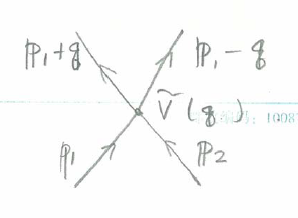
\includegraphics[width = 4.6cm]{1-4.png}
\end{wrapfigure}

where

\[\tilde{V}({\bf q})\equiv\int d^3{\bf x}V({\bf x})e^{_i\bf q\cdot x} \]

Note that this adds momentum $\bf q$ to one particle while substracts the same momentum $\bf q$ from the other with the amplitude of $\tilde{V}({\bf q})$

\begin{align}
\hat{V}|{\bf p}_1,{\bf p}_2\rangle = \frac{d\bf q}{(2\pi)^3}\tilde{V}({\bf q})|{\bf p}_1+{\bf q,p}_2-{\bf q}\rangle
\end{align}

This process is denoted by this diagram which is often called as Feynman diagram. 

\section{Degenerate electron gas}

So far, we have reviewed the $2$nd quantization. From the nextt weeks, we will study interacting fermi systems using $2$nd quantization Language. More specifically, we will often study a simple model that provides a first approximation to a metal. This system is an interacting electron gas placed in a uniformly distributed positive background. Because of the positive background, the total system is ensured to be neutral. In a real metal, the positive charge is localized in the ionic cores, whose dynamical motion must also be included in the calculation. 

However, these positive ions are usually much heavier than the electrons, so that it is permissible to neglect to ionic motions entirely. In contrast, the assumption of a uniform background is more drastic. In this sense, the present model can provide only a qualitative account of real metals in solids. 

We are interested in the properties of the bulk medium. Thus, it is convenient to enclose the system in a large cubic box with sides of length ``$L$''. The limit $L\rightarrow\infty$ will be taken at the end of the calculation. 

In a uniform infinite medium, all the physical properties must be invariant under spatial translation. This observation suggests the use of periodic boundary condition on the single-particle state;

\begin{align}
psi_{k,\lambda}({\bf x}) = \frac{1}{\sqrt{V}}e^{i\bf k\cdot x}\eta_{\lambda}
\end{align}

$V(\equiv L^3)$ is the volume of the box, $\eta_\lambda$ with $\lambda = \uparrow,\downarrow$ are the two spin functions for spin-up and spin-down

\begin{align}
\eta_\uparrow = \left(\begin{matrix}1\\0\end{matrix}\right),\eta_\downarrow = \left(\begin{matrix}0\\1\end{matrix}\right)
\end{align}

The periodic boundary condition determines the allowed wavelengths as

\begin{align}
{\bf k} = \frac{2\pi}{L}(n_x,n_y,n_z)
\end{align}

with $n_x,n_y,n_x = 0,\pm1,\pm2,\cdots,\pm\frac{L}{2}$. 

The total Hamiltonian of the system consists of three terms:

\begin{align}
H = H_el+H_b+H_{el-b}
\end{align}

where $H_{el}$ is the hamiltonian for the electrons:

\begin{align}
H_{el} = \sum_{i=1}^N\frac{P_i^2}{2m}+\frac{e^2}{2}\sum_{i\neq j}^N\frac{e^{-\mu|{\bf r}_i - {\bf r}_j|}}{|{\bf r}_i - {\bf r}_j|}
\end{align}

$H_b$ is the energy of the positive background whose particle density is $n(\bf x)$

\begin{align}
H_b = \frac{e^2}{2}\iint d^3{\bf x}d^3{\bf x'}\frac{n({\bf x})n({\bf x'})e^{-\mu|\bf x-x'|}}{|\bf x-x'|}
\end{align}

$H_{el-b}$ is the interaction energy between the electrons and the positively charged background

\begin{align}
H_{el-b} = -e^2\sum_{i=1}^N\int d^3{\bf x}\frac{n({\bf x})e^{-\mu|{\bf x-r}_i|}}{|{\bf x - r}_i|}
\end{align}

We have inserted an exponential convergence factor $\mu$ to define the integrals and this $\mu$ will be taken to be zero in the very end of the analysis. Because of the long-range nature of the coulomb interaction, these three terms ``individually'' diverge in the thermodynamics limit

($N\rightarrow\infty, V\rightarrow\infty$ with $n = N/V$ fixed)

However, the entire system is electrically neutral, so that the sum of these three terms must remains finite and meaningful in this limit. 

The convergence factor $\mu$ allows us to make this cancellation explicitly. 

Thus, our limiting procedure is firstly take the thermodynamic limit 

($N\rightarrow\infty, V\rightarrow\infty$ with $n = N/V$ fixed)

and then take $\mu\rightarrow0$. 

Equivalently, we can assume that $\mu^{-1}\ll L$ at each step of our following calculation. 

Now that the positive background $n(\bf x)$ is static, $H_b$ is a pure $c$-number, which can be easily evaluated for a uniform distribution of $n({\bf x})\equiv\frac{N}{V}$

\begin{align}
\begin{split}
H_b &=\frac{e^2}{2}\left(\frac{N}{V}\right)^2\iint d^3{\bf x}d^3{\bf x'}\frac{e^{-\mu|\bf x-x'|}}{|\bf x-x'|}\\
&=\frac{e^2}{2}\left(\frac{N}{V}\right)^2\int d^3{\bf x}\int d^3{\bf x}\frac{e^{-\mu|\bf z|}}{|\bf x|}
\end{split}
\end{align}%page99

Here we shifted the origin of the integration in the second line, which is allowed since $\mu^{-1}\ll L$. 

$N^{-1}\cdot H_b$ diverges in the limit of $\mu\to +0$, which represents the long-range nature of the coulomb interaction. 

$H_{el-b}$ is a one-particle operator for electron for static background $n({\bf x})$. 

For the uniform distribution, we may again use the translation invariant to estimate this as a $c$-number:

\begin{align}
\begin{split}
H_{el-b}&=-e^2\sum_{i=1}^N\frac{N}{V}\int d^3{\bf x}\frac{e^{-\mu|{\bf x-r}_i|}}{|{\bf x-r}_i|}\\
&=-e^2\sum_{i=1}^N\frac{N}{V}\int d^3{\bf x}\frac{e^{-\mu|{\bf x}}}{|{\bf x}|}\\
&=-e^2\frac{N^2}{V}\frac{4\pi}{\mu^2}
\end{split}
\end{align}

Thus the total Hamiltonian becomes 

\begin{align}\label{eq1.8.10}
\hat{H}=-\frac{e^2}{2}\frac{N^2}{V}\frac{4\pi}{\mu^2}+\hat{H}_{el}
\end{align}

so that all of the interacting physical effects are contained in $\hat{H}_{el}$. 

We now rewrite $H_{el}$ in terms of the $2$nd quantization language. We use a basis of momentum eigenstate with spin degree of freedom:

\[\psi_{{\bf k},\lambda}({\bf x})=\frac{1}{\sqrt{V}}e^{i\bf k\cdot x}\eta_\lambda \]

with $\lambda=\uparrow$ or $\downarrow$ \& ${\bf k}=\frac{2\pi}{L}(n_x,n_y,n_z)$

Correspongding creation \& annihilation operator has momentum \& spin indies, 

\[
\left.\begin{matrix}
a^\dagger_{{\bf k},\lambda} \\
\ \\
\underset{\text{momentum,spin}\quad}{a^\dagger_{{\bf k},{\lambda}}}
\end{matrix}\right\}\longrightarrow\psi_{{\bf k},\lambda}({\bf x})=\frac{1}{\sqrt{V}}e^{i\bf k\cdot x}\eta_\lambda 
\]

Moreover, the inner product between these `single-particle states' is given by

\[\begin{split}
\langle {\bf k},\lambda|{\bf k'},\lambda\rangle&\equiv\frac{1}{V}\int_V d^3{\bf x}\psi_{{\bf k},\lambda}^*({\bf x})\psi_{{\bf k'},\lambda'}({\bf x}) \\
&=\delta_{\lambda,\lambda'}\frac{1}{V}\int_V d^3{\bf x}e^{-i\bf (k-k')\cdot x}\\
&=\delta_{\lambda,\lambda'}\delta_{\bf k,k'}
\end{split}\]

with $\delta_{\bf k,k'}\equiv\delta_{n_x,n_x'}\delta_{n_y,n_y'}\delta_{n_z,n_z'}$

so that eq. \eqref{eqs1.6.5} tells that

\[[a_{{\bf k},\lambda},a^\dagger_{{\bf k'},\lambda}]\equiv\delta_{\lambda,\lambda'}\delta{\bf k,k'} \]

\dotfill

\ 

On the one hand, eq. \eqref{eqs1.7.6} suggests that the kinetic energy part is given by

\[\hat{T}\equiv\sum_{{\bf k}\lambda}\sum_{{\bf k'},\lambda'}a^\dagger_{{\bf k}\lambda} a_{{\bf k'},\lambda'}\langle{\bf k}\lambda|T|{\bf k'},\lambda'\rangle\]

where

\begin{align}\label{eq1.8.11}
\begin{split}
\langle{\bf k}\lambda|T|{\bf k'},\lambda'\rangle&\equiv\frac{\delta_{\lambda,\lambda'}}{V}\int d^3{\bf x}e^{-i\bf k\cdot x}\left(-\frac{\hbar^2\nabla^2}{2m}\right)e^{i\bf k'\cdot x}\\
&=\frac{\hbar^2 k^2}{2m}\delta_{\bf k,k'}\delta_{\lambda,\lambda'}\\
&\equiv\sum_{{\bf k},\lambda}\frac{\hbar^2\bf k^2}{2m}a^\dagger_{{\bf k}\lambda}a_{{\bf k}\lambda}
\end{split}
\end{align}

The two-particle interaction part can be evaluated from eq. \eqref{eqs1.7.18} as

\[\begin{split}
V=&\frac{e^2}{2}\int_V d^3{\bf x}\int_V d^3{\bf y}\sum_{\tau,\tau'}\frac{e^{-\mu|\bf x-y|}}{|\bf x-y|}\left( \sum_{{\bf k}_1,\lambda_1}\psi^*_{{\bf k}_1,\lambda_1}({\bf x},\tau)a_{{\bf k}_1,\lambda_1}^\dagger\right)\times\left( \sum_{{\bf k}_2,\lambda_2}\psi^*_{{\bf k}_2,\lambda_2}({\bf y},\tau')a_{{\bf k}_2,\lambda_2}^\dagger\right)\\
&\times\left( \sum_{{\bf k}_4,\lambda_4}a_{{\bf k}_4,\lambda_4}\psi_{{\bf k}_4,\lambda_4}({\bf y},\tau')\right)\times\left( \sum_{{\bf k}_3,\lambda_3}a_{{\bf k}_3,\lambda_3}\psi_{{\bf k}_3,\lambda_3}({\bf x},\tau)\right)
\end{split}\]

Since we consider a spinful fermion here, 

\[\int d^3{\bf x}\int d^3{\bf y}a^\dagger({\bf x})a^\dagger({\bf y})a({\bf y})a({\bf x})V^{(2)}({\bf x,y})\to\sum_\tau \sum_{\tau'}\int d^3{\bf x},\tau)a^\dagger({\bf y},\tau')a({\bf y},\tau')a({\bf x},\tau)\times V^{(2)}(\bf x,y)\]

We changed the single particle basis from coordinate to momentum

\[\begin{cases}
a^\dagger({\bf x},\tau)&=\sum_{{\bf k}\lambda}\psi_{{\bf k},\lambda}^*({\bf x},\tau)a^\dagger_{{\bf k},\lambda}\\
\ & \\
a({\bf x},\tau)&=\sum_{{\bf k'}\lambda'}\psi_{{\bf k'},\lambda'}({\bf x},\tau)a_{{\bf k'},\lambda'}
\end{cases}\]

\[V=\frac{1}{2}\sum_{{\bf k}_1,\sim,{\bf k}_4}\sum_{\lambda_1,\sim,\lambda_4}\langle{\bf k}_1,\lambda_1,{\bf k}_2,\lambda_2|V|{\bf k}_4,\lambda_4,{\bf k}_3,\lambda_3\rangle\times a^\dagger_{{\bf k}_1,\lambda_1}a^\dagger_{{\bf k}_2,\lambda_2}a_{{\bf k}_4,\lambda_4}a_{{\bf k}_3,\lambda_3}\]

where

\[\begin{split}
\langle{\bf k}_1,\lambda_1,{\bf k}_2,\lambda_2|V|{\bf k}_4,\lambda_4,{\bf k}_3,\lambda_3\rangle &=\frac{e^2}{V}\iint d^3{\bf x}d^3{\bf y}\sum_{\tau}\sum_{\tau'}e^{-i{\bf k}_1\cdot\bf x}\eta_{\lambda_1}^\dagger(\tau)e^{_i{\bf k}_2\cdot\bf y}\eta_{\lambda_2}^\dagger(\tau')\frac{e^{-\mu|\bf x-y|}}{|\bf x-y|}e^{-{\bf k}_4\cdot\bf y}\eta_{\lambda_4}(\tau')e^{i{\bf k}_3\cdot\bf x}\eta_{\lambda_3}(\tau)\\
&=\frac{e^2}{V^2}\int d^3{\bf y}e^{-i({\bf k}_1 + {\bf k}_2 - {\bf k}_3 - {\bf k}_4)\cdot\bf y}\times\int d^3{\bf x}e^{i({\bf k}_3-{\bf k}_1)\cdot\bf x}\frac{e^{-\mu|\bf x|}}{|\bf x|}\delta_{\lambda_1,\lambda_3}\delta_{\lambda_2,\lambda_4}\\
&=\frac{e^2}{V}\delta_{\lambda_1,\lambda_3}\delta_{\lambda_2,\lambda_4}\delta_{{\bf k}_1 + {\bf k}_2,{\bf k}_3 + {\bf k}_4}\times\frac{4\pi}{({\bf k}_1 - {\bf k}_3)^2+\mu^2}
\end{split}\]

Thus, with ${\bf k}_1 - {\bf k}_3 = \bf q$, we have

\begin{align}
\hat{V}=\frac{e^2}{2V}\sum_{\bf k,p,q}\sum_{\lambda_1,\lambda_2}\frac{4\pi}{{\bf q^2}+\mu^2}a^\dagger_{{\bf k+q},\lambda_1}a^\dagger_{{\bf p-q},\lambda_2}a_{{\bf p},\lambda_2}a_{{\bf k},\lambda_1}
\end{align}

It is convenient to separate the summation over $\bf q$ into two parts

\begin{align}\label{eq1.8.13}
V=\frac{e^2}{2V}\sum_{\bf k,p}\sum_{{\bf q}\neq0}\sum_{\lambda_1,\lambda_2}\frac{4\pi}{{\bf q^2}+\mu^2}a^\dagger_{{\bf k+q},\lambda_1}a^\dagger_{{\bf p-q},\lambda_2}a_{{\bf p},\lambda_2}a_{{\bf k},\lambda_1} + \frac{e^2}{2V}\sum_{\bf k,p}\sum_{\lambda_1,\lambda_2}\frac{4\pi}{\mu^2}a^\dagger_{{\bf k},\lambda_1}a^\dagger_{{\bf p},\lambda_2}a_{{\bf p},\lambda_2}a_{{\bf k},\lambda_1}
\end{align}

where the first term refers to $\bf q\neq0$ while the second term refers to $\bf q=0$. The second term can be further evaluated as 

\[\text{second term}= \frac{e^2}{2V}\sum_{\bf k,p}\sum_{\lambda_1,\lambda_2}\frac{4\pi}{\mu^2}a^\dagger_{{\bf k},\lambda_1}a_{{\bf k},\lambda_1}(a^\dagger_{{\bf p},\lambda_2}a_{{\bf p},\lambda_2}-\delta_{\bf k,p}\delta_{\lambda_1,\lambda_2}) = \frac{e^2}{2V}\frac{4\pi}{\mu^2}(\hat{N}^2-\hat{V})\]

where $\hat{N}\equiv\sum_{{\bf k}\lambda}a_{{\bf k},\lambda}^\dagger a_{{\bf k},\lambda}$ is an operator representing the total number of electrons (see eq. \eqref{eqs1.7.15} also). 

In a sub-Hilbert space of fixed number of electrons, we can replace this by a $c$-number $N$ so that the $2$nd term reduces to a $c$-number

\[\text{second term}=\frac{e^2}{2}\frac{N^2}{V}\frac{4\pi}{\mu^2}-\frac{e^2}{2}\frac{N}{V}\frac{4\pi}{\mu^2}\]

putting this into eq. \eqref{1.8.13} abd substituting eqs. \eqref{eq1.8.13} \& \eqref{eq1.8.11} into eq. \eqref{eq1.8.10}, we finally have

\[\hat{H}=-\frac{e^2}{2}\frac{N^2}{V}\frac{4\pi}{\mu^2}+\sum_{{\bf k},\lambda}\frac{\hbar^2\bf k^2}{2m}a^\dagger_{{\bf k},\lambda}a_{{\bf k},\lambda}+\frac{e^2}{2V}\sum_{\bf k,p} \sum_{{\bf q}\neq0}\sum_{\lambda_1,\lambda_2}\frac{4\pi}{{\bf q^2}+\mu^2}a^\dagger_{{\bf k+q},\lambda_1}a^\dagger_{{\bf p-q},\lambda_2}a_{{\bf p},\lambda_2}a_{{\bf k},\lambda_1} + \frac{e^2}{2}\frac{N^2}{V}\frac{4\pi}{\mu^2}-\frac{e^2}{2}\frac{N}{V}\frac{4\pi}{\mu^2} \]

The last term represents an energy per particlem $-\displaystyle\frac{e^2}{2}\frac{4\pi}{V\mu^2}$, which vanished in the thermodynamic limit with $\mu^{-1}\ll L$. 

Therefore, it is now clear that these two terms, each of which diverges in the limit of $\mu\to0$ respectively, cancel each other, so that the entire Hamiltonian has no trivially diverging term. This comes from the electric neutrality of the entire system. 

Furthermore, it is now permissible to set $\mu=0$ here, because this summation excludes $\bf q=0$ and the summand is always well defined even at $\mu =0$. 

We thus reach the final Hamiltonian for a bulk electron gas in a uniformly distributed positively-charged background. 

\begin{align}\label{eq1.8.14}
\hat{H}=\sum_{{\bf k},\lambda}\frac{\hbar^2\bf k^2}{2m}a^\dagger_{{\bf k},\lambda}a_{{\bf k},\lambda} + \frac{e^2}{2V}\sum_{\bf k,p} \sum_{{\bf q}\neq0}\sum_{\lambda_1,\lambda_2}\frac{4\pi}{{\bf q^2}}a^\dagger_{{\bf k+q},\lambda_1}a^\dagger_{{\bf p-q},\lambda_2}a_{{\bf p},\lambda_2}a_{{\bf k},\lambda_1}
\end{align}

where the limit $N\to\infty, V\to\infty$ with $N/V=n=$constant is implicitly assumed. 

We often call this model as a model of degenerate electron gas or a model for Fermi gas with long-range Coulomb interaction. This model is a prototype model for studying the physical properties of a metal in solids. 

\dotfill

\ 

From the next class, I will go to $\cdots$ general theory framework for many-body systems, especially focusing on interacting fermion systems. 
\chapter{Green's function and field theory at zero temperature}
In most cases of interest, the first few orders of perturbation theory cannot provide an adequate description of an interacting many-particle system.

 For this reason, we need to develop systematic methods for solving Shrodinger equation to all orders in perturbation theory.

\section{Schrodinger, Heisenberg \& interaction picture}

In most cases of interest, the first few orders of perturbation theory cannot provide an adequate description of an interacting many-particle system.

 For this reason, we need to develop systematic methods for solving Shrodinger equation to all orders in perturbation theory.


As a preliminary step, we will brief review three important representation, that are useful in analyzing the 2nd-quantized form of the schrodinger equation.

 The usual description of quantum mechanics assumes that the state vectors are time-dependent, while the operators are time-independent.

\begin{align}
\bm{i} \hbar \frac{\partial}{\partial t} | \Psi_S(t)\rangle=\hat{H}| \Psi_S(t)\rangle \nonumber \\
or\left(| \Psi_S(t)\rangle=e^{-\bm{i}\hat H \frac{t'-t_0}{\hbar}}\right) \nonumber \\
\bm{i} \hbar \frac{\partial}{\partial t} \hat O_s = 0 \nonumber
\end{align}
 This picture is called Schrodinger picture.

 The other representation is called Heisenberg picture, in which the state vector is time-independent and the operators are time-dependent.

\begin{align}
| \Psi_H(t)\rangle=e^{\bm{i}  \frac{\hat Ht}{\hbar}}| \Psi_S(t)\rangle  \\
or\left( \bm{i} \hbar \frac{\partial}{\partial t}| \Psi_H(t)\rangle=0\right) \nonumber \\
\hat O_H(t) \equiv e^{\bm{i}  \frac{\hat Ht}{\hbar}}\hat O_S e^{-\bm{i}  \frac{\hat Ht}{\hbar}} \\
or \left( \bm{i} \hbar \frac{\partial}{\partial t}  O_H(t)=[ O_H(t), \hat H] \right)\nonumber
\end{align}

 By construction, an arbitrary matrix element calculated in the Schrodinger picture and that in the Heisenberg picture gives same answer.
\begin{align}
\langle\Psi_S'(t)|O_S|\Psi_S(t)\rangle=\langle\Psi_H'|e^{\bm{i}  \frac{\hat Ht}{\hbar}}O_Se^{-\bm{i}  \frac{\hat Ht}{\hbar}}|\Psi_H\rangle \nonumber
\end{align}
 The third description is called "interaction picture", in which bothe the state vectors and the operators are time-dependent.

 But the time-dependence of the state vectors is determined by some part of the Hamiltonian, while that of the operator is determined by the other part of the Hamiltonian.

 To see this, assume  that the Hamiltonian can be expressed as the sum of two parts.

\begin{align}
\hat H=\hat H_0+\hat H_1 \nonumber
\end{align}

  where $\hat H_0$ and $\hat H_1$ generally don't commute.

 $\hat H_0$ alone yields a soluble problem, whose eigenstates are comletely understood.

 Examples of $\hat H_0$ is Eq.(1.7.13), and 1st term of Eq.(1.8.14).

 The combination of $\hat H_0$ \& $\hat H_1$ yields a non-soluble problem, where the examples of $\hat H_1$ is the two-body interaction potentials such as Eq.(1.7.18) and 2nd term of Eq.(1.8.14).

 $\hat H_1$ is called the interaction part, while $\hat H_0$ is called the non-interaction part.

 state-vector in the interaction representation is defined as
\begin{align}
|\Psi_I(t)\rangle \equiv e^{\bm{i}  \frac{\hat H_0t}{\hbar}}|\Psi_S(t)\rangle
\end{align}
so that its time-dependence is determined by the interaction part.

\begin{align}
\bm{i} \hbar \frac{\partial}{\partial t} |\Psi_I(t)\rangle & =  -\hat H_0 e^{\bm{i}  \frac{\hat H_0t}{\hbar}}|\Psi_S(t)\rangle+e^{\bm{i}  \frac{\hat H_0t}{\hbar}}|\Psi_S(t)\rangle \nonumber \\
& =  e^{\bm{i}  \frac{\hat H_0t}{\hbar}}(-\hat H_0+\hat H_0+\hat H_1)e^{-\bm{i}  \frac{\hat H_0t}{\hbar}} |\Psi_I(t)\rangle \nonumber \\
& =  \hat H_1(t)|\Psi_I(t)\rangle  \\
(\hat H_1(t) &  \equiv e^{\bm{i}  \frac{\hat H_0t}{\hbar}}\hat H_1 e^{-\bm{i}  \frac{\hat H_0t}{\hbar}}  ) \nonumber
\end{align}
 An operator in the interaction picture is given by 
\begin{align}\label{2-1-5}
\hat O_I(t) \equiv e^{\bm{i}  \frac{\hat H_0t}{\hbar}}\hat O_S e^{-\bm{i}  \frac{\hat H_0t}{\hbar}}
\end{align}
so that an arbitrary matrix element calculated in the other pictures becomes identical to that in the interaction picture.
\begin{align}
\langle\Psi_S'(t)|O_S|\Psi_S(t)\rangle=\langle\Psi_I'|O_I|\Psi_I\rangle \nonumber
\end{align}

 The important point here is that the time-dependence of the operators in
the interaction picture is determined only by the non-interacting part.
\begin{align}
\bm{i} \hbar \frac{\partial}{\partial t} \hat O_I(t) &= e^{\bm{i}  \frac{\hat H_0t}{\hbar}}(\hat O_S \hat H_0 - \hat H_0\hat O_S) e^{-\bm{i}  \frac{\hat H_0t}{\hbar}} \nonumber \\
&=[\hat O_I(t), \hat H_0] \nonumber
\end{align}

 Because of this, the time-dependence of the operators becomes particularly simple in the interaction picture.

 For example, consider a representation in which $\hat H_0$ is diagonal,
\begin{align}
\hat H_0= \sum_k \hbar \epsilon_k c_k^{\dagger} c_k \nonumber
\end{align}

 The time-dependence of the creation and destruction operators are given by,
\begin{align}
\bm{i} \hbar \frac{\partial}{\partial t} \hat c_{k,I}(t) &= e^{\bm{i}  \frac{\hat H_0t}{\hbar}}[\hat c_{k,S}(t), \hat H_0] e^{-\bm{i}  \frac{\hat H_0t}{\hbar}} \nonumber \\
&=\hbar \epsilon_k c_{k,I}(t) \nonumber
\end{align}
which yields
\begin{align}
c_{k,I}(t)&\equiv c_k e^{-\bm{i}\epsilon_kt} \nonumber \\
c_{k,I}^{\dagger}(t)&= c^{\dagger}_k e^{-\bm{i}\epsilon_kt} \nonumber
\end{align}

 Since any operators in Schrodinger picture is expressed in terms of the complete set of $c_k \& c^{\dagger}_k$, the corrsponding operator in the interaction picture is obtained with the simple replacement of $c_k \& c^{\dagger}_k$ by $c_{k,I}(t) \& c^{\dagger}_{k,I}(t)$;

\begin{align}
\hat O_S \equiv f(\hat c_{k_1},\hat c^{\dagger}_{k_1},\hat c_{k_2},\hat c^{\dagger}_{k_2},...)\nonumber
\end{align}
\begin{align}
\hat O_I(t) \equiv f(\hat c_{k_1,I},\hat c^{\dagger}_{k_1,I},\hat c_{k_2,I},\hat c^{\dagger}_{k_2,I},...)\nonumber
\end{align}
f is an arbitrary function.

 Then we will now try to solve the equations of motion for the state vector.

 Let me first define a unitary operator at time t in terms of the state vector at the time $t_0$.
\begin{align}
|\Psi_I(t)\rangle=\hat U(t,t_0)|\Psi_I(t_0)\rangle
\end{align}
with $\hat U(t_0,t_0)=1$

 The unitary operator can be calculated explicitly,
\begin{align}
|\Psi_I(t)\rangle& =e^{\bm{i}  \frac{\hat H_0t}{\hbar}}|\Psi_S(t)\rangle \nonumber \\
&= e^{\bm{i}  \frac{\hat H_0t}{\hbar}}e^{-\bm{i}  \frac{\hat H_(t-t_0)}{\hbar}}|\Psi_S(t_0)\rangle \nonumber \\& = e^{\bm{i}  \frac{\hat H_0t}{\hbar}}e^{-\bm{i}  \frac{\hat H_(t-t_0)}{\hbar}}e^{-\bm{i}  \frac{\hat H_0t_0}{\hbar}}|\Psi_I(t_0)\rangle \nonumber
\end{align}
From where we obtain
\begin{equation} \tag{2.1.6'}
\hat{U}(t,t_0)=e^{\bm{i}H_0t/\hbar}e^{-\bm{i}H(t-t_0)/\hbar}e^{-\bm{i}H_0t_0/\hbar} \nonumber
\end{equation}
 This symbolic expression gives us several general properties of the unitary operators;
\begin{align}
\hat{U^{\dagger}}(t,t_0)\hat{U}(t,t_0)&=\bm{1} \nonumber\\
\hat{U}(t_1,t_2)\hat{U}(t_2,t_3)&=\hat{U}(t_1,t_3)\nonumber
\end{align}
so that 
\begin{align}
\hat{U}(t,t')\hat{U}(t',t)&=\bm{1} \nonumber \\
\hat{U^{\dagger}}(t,t') & \equiv \hat{U}(t',t) \nonumber
\end{align}
 Although this expression is the formal solution to the problem, it is very useful for the computation purpose.

 In the following, I will construct an integral equation of $\hat{U}$, which can be solved iteratively.

 Comparing eq.(2.1.6) \& eq.(2.1.4), we have
\begin{align}\tag{2.1.6''}
\bm{i}\hbar \frac{\partial}{\partial t} \hat{U}(t,t_0)=\hat{H_1}(t)\hat{U}(t,t_0) \nonumber
\end{align}

 Integrating this from $t_0$ to $t$, we have 
\begin{align}
\hat{U}(t,t_0)-\hat{U}(t_0,t_0)=-\bm{i}/\hbar \int_{t_0}^{t} \hat{H_1}(t')\hat{U}(t',t_0) \nonumber
\end{align}

 where we can replace this by $\hat{\bm{1}}$

 This leads to an integral equation!
\begin{equation}
\hat{U}(t,t_0)=\hat{\bm{1}}-\bm{i}/\hbar \int_{t_0}^{t} \hat{H_1}(t')\hat{U}(t',t_0) \nonumber
\end{equation}

 By substituting the left-hand side into the integrant in the right hand side, one obtain an interative solution for this.
\begin{align}
\hat{U}(t,t_0)=\hat{\bm{1}} &+(-\bm{i}/\hbar) \int_{t_0}^{t} \hat{H_1}(t')\bm{d}t' \nonumber\\
&+(-\bm{i}/\hbar)^2\int_{t_0}^{t}\bm{d}t'\int_{t_0}^{t'}\bm{d}t''\hat{H_1}(t')\hat{H_1}(t'')\nonumber\\
&+(-\bm{i}/\hbar)^3  \int_{t_0}^{t}\bm{d}t'\int_{t_0}^{t'}\bm{d}t''\int_{t_0}^{t''}\bm{d}t'''\hat{H_1}(t')\hat{H_1}(t'')\hat{H_1}(t''')+...... \nonumber
\end{align}
The third term may be rewritten as
\begin{align}
&\int_{t_0}^{t}\bm{d}t'\int_{t_0}^{t'}\bm{d}t''\hat{H_1}(t')\hat{H_1}(t'')\nonumber\\
&=\frac{1}{2}\int_{t_0}^{t}\bm{d}t'\int_{t_0}^{t'}\bm{d}t''\hat{H_1}(t')\hat{H_1}(t'')+\frac{1}{2}\int_{t_0}^{t}\bm{d}t''\int_{t''}^{t}\bm{d}t'\hat{H_1}(t')\hat{H_1}(t'')\nonumber
\end{align}
where I reverse the order of the integration in the last term.

 Then we interchange the dummy variable $t'$ \& $t''$ in the second term.
\begin{align}
=...+\frac{1}{2}\int_{t_0}^{t}\bm{d}t'\int_{t''}^{t}\bm{d}t''\hat{H_1}(t'')\hat{H_1}(t')\nonumber
\end{align}
 These two can be recombined again
\begin{align}
=...+\frac{1}{2}\int_{t_0}^{t}\bm{d}t'\int_{t''}^{t}\bm{d}t''[\hat{H_1}(t')\hat{H_1}(t'')\theta(t'-t'')+\hat{H_1}(t'')\hat{H_1}(t')\theta(t''-t')]\nonumber
\end{align}
where $\theta(t)$ is the step function.
\begin{eqnarray}
\theta(x)\equiv
\begin{cases}
1, &t>0 \cr 0, &t<0\end{cases} \nonumber
\end{eqnarray}
 Note also that these two do not commute with each other in general.

 Thus, you cannot rewrite this into
\begin{align}
\hat{H_1}(t')\hat{H_1}(t'')[\theta(t'-t'')+\theta(t''-t')] \nonumber
\end{align}

 This expression has the characteristic feature that the operator containing the latest  time appears to the left.

 We call this a "time-ordered product of operator" denoted by "T".
\begin{align}
\frac{1}{2}\int_{t_0}^{t}\bm{d}t'\int_{t_0}^{t}\bm{d}t''\bm{T}[\hat{H_1}(t')\hat{H_1}(t'')]\nonumber
\end{align}

 More generally, one can rewrite n-th order term in this iterative series in terms of the "time-ordered product".

\begin{align}\label{2-1-7}
&\int_{t_0}^{t}\bm{d}t_1\int_{t_0}^{t_1}\bm{d}t_2......\int_{t_0}^{t_{n-1}}\bm{d}t_n \hat{H_1}(t_1)\hat{H_1}(t_2)......\hat{H_1}(t_n)\nonumber \\
&= \frac{1}{n!}\int_{t_0}^{t}\bm{d}t_1\int_{t_0}^{t_1}\bm{d}t_2......\int_{t_0}^{t_{n-1}}\bm{d}t_n\bm{T}[\hat{H_1}(t_1)\hat{H_1}(t_2)......\hat{H_1}(t_n)]
\end{align}
where
\begin{align}
&\bm{T}[\hat{A}(t_1)\hat{B}(t_2)\hat{C}(t_3)] \nonumber \\
&=\theta(t_1-t_2)\theta(t_2-t_3)\hat{A}(t_1)\hat{B}(t_2)\hat{C}(t_3) \nonumber \\
&=\theta(t_1-t_3)\theta(t_3-t_2)\hat{A}(t_1)\hat{B}(t_3)\hat{C}(t_2) \nonumber \\
&=\theta(t_2-t_1)\theta(t_1-t_3)\hat{A}(t_2)\hat{B}(t_1)\hat{C}(t_3) \nonumber \\
&+ ... \nonumber
\end{align}

 Thus, this unitary operator becomes
\begin{align}
\hat{U}(t,t_0)&\equiv\sum_{n=0}^{\infty}(-\bm{i}/\hbar)^n\frac{1}{n!}\int_{t_0}^{t}\bm{d}t_1\int_{t_0}^{t_1}\bm{d}t_2......\int_{t_0}^{t_{n-1}}\bm{d}t_n\bm{T}[\hat{H_1}(t_1)\hat{H_1}(t_2)......\hat{H_1}(t_n)] \nonumber \\
&=\bm{T} \{exp[(-\bm{i}/\hbar)\int_{t_0}^{t}\bm{d}t'\hat{H_1}(t')]\}
\end{align}

 	Comparing eq.(2.1.5)\&(2.1.2), (2.1.3)\&(2.1.1), we can relate the Heisenberg picture \& the interaction picture.
\begin{align}
\hat{O_H}(t)&=e^{\bm{i}Ht/\hbar}e^{-\bm{i}H_0t/\hbar}\hat{O_I}(t)e^{\bm{i}H_0t/\hbar}e^{-\bm{i}Ht/\hbar} \nonumber \\
&=\hat{U}(0,t)\hat{O_I}(t)\hat{U}(t,0) \nonumber \\
|\Psi_H\rangle&=\hat{U}(0,t)|\Psi_I(t)\rangle \nonumber \\
&=\Psi_I(t=0)\rangle
\end{align}







\section{Adiabatic switching \& Gell-Mann \& Low Theorem}

``Adiabatic switching'' is a gedenken experimental process, in which the interaction part of the Hamiltonian is adiabatically switched on. This process is a mathematical device that generate exact eigenstates of the interacting system from those of the non-interacting system. 

Specifically, we consider a new Hamiltonian:

\[\hat{H}=\hat{H}_0+e^{-\epsilon|t|}\hat{H}_1 \]

where $\epsilon$ is a small positive value. 

When the time goes $+$ infinity ot $-$ infinity, the Hamiltonian reduces to $\hat{H}_0$, which is a soluble limit. At $t=0$, $\hat{H}$ becomes the full Hamiltonian of the interacting systems. We will take $\epsilon$ to be zero at the end of the calculation, which means that the interaction part is turned on and off inginitely slowly or adiabatically. 

Any meaning calculation results should be free from $\epsilon$. 

Even when $\hat{H}_1$ is time-dependent in the Schr\"{o}dinger picture, Eqs. \eqref{2-1-5} \& \eqref{2-1-7} remain correct:

\begin{align}
|\Psi_I(t)\rangle=\hat{U}_\epsilon(t,t_0)|\Psi_I(t_0)\rangle
\end{align}

\begin{align}\label{2-2-2}
\hat{U}_\epsilon(t,t_0)&=\sum_{n=0}^{+\infty}\left(\frac{-i}{\hbar}\right)^n\frac{1}{n!}\int_{t_0}^t dt_1 \cdots \int_{t_0}^t dt_n\times e^{-\epsilon(|t_1|+\cdots+|t_n|)}\times\\
\nonumber&{\color{red}{T[\hat{H}_{(t_1)}\cdot\cdots\cdot\hat{H}_1(t_n)]}}\\
\nonumber&\left(\text{which equals to\ }\sum_P\theta(t_{p(1)}-t_{p(2)})\cdot\theta(t_{p(2)}-t_{p(3)})\cdots\theta(t_{p(n-1)}-t_{p(n)}) \hat{H}_{(t_{p(1)})}\cdot\cdots\cdot\hat{H}_1(t_{p(n)})\right)
\end{align}


%133

When ``$t_0$'' approaches - infinity, $\hat{H}$ become $\hat{H}_0$, the state vector in the Schr?dinger picture reduces to

\[|\Psi_S(t_0)\rangle = e^{-i E_0 t_0/\hbar}|\Phi_0\rangle \]

where $|\Psi_0\rangle$ is time-independent stationary eigenstate of the unperturbed Hamiltonian

\[|H_0|\Psi_0\rangle = E_0|\Phi_0\rangle\]

Then, corresponding state vector in the interaction becomes interaction becomes 

\[\lim_{t_0\to-\infty}|\Psi_I(t_0)\rangle = e^{i H_0t_0/\hbar}|\Psi_S(t_0)\rangle = |\Phi_0\rangle \]

Using eq. (i), we obtain

\[|\Psi_I(0)\rangle = U_\epsilon (0,-\infty)|\Psi_0\rangle \]

Gell-Mann and Low Theorem suggests that this state is an exact eigenstate of the interacting system. 

More accurately, the theorem is stated as follows. 

If this quantity exists to all orders in perturbation theory

\[\lim_{\epsilon\to0}\frac{\hat{U}_\epsilon(0,-\infty)|\Phi_0\rangle}{\langle\Phi_0|\hat{U}_\epsilon(0,-\infty)|\Phi_0\rangle} \equiv \frac{|\Psi_0\rangle}{\langle\Phi_0|\Psi_0\rangle} \]

then, this state is a eigenstate of $H$

\begin{align}
H\frac{|\Psi_0\rangle}{\langle\Phi_0|\Psi_0\rangle} = E\frac{|\Psi_0\rangle}{\langle\Phi_0|\Psi_0\rangle}
\end{align}

An essential point of the theorem is that the numerator and the denominator of this equation do not separately exists in the limit of $\epsilon\to0$. 

In this limit, the phase of the numerator diverges like $\epsilon^{-1}$ and the denominator also does so as to set off the infinite phase in the numerator. 

Namely, the theorem stats that, if the ratio exists (does not contain any infinite phase), the eigenstate is well-defined and has the eigenvalue of the interacting system. 

To prove this statement, consider first the expression

\[(\hat{H}_0-E_0)|\Psi_0(\epsilon)\rangle = (\hat{H}_0-E_0)\hat{U}_\epsilon(0,-\infty)|\Phi_0\rangle = \left\{\hat{H}_0\hat{U}_\epsilon(0,-\infty)-\hat{U}_\epsilon(0,-\infty)\hat{H}_0\right\}|\Phi_0\rangle \]

To evaluate the commutator, consider the $n$-th term in equation \eqref{2-2-2} for $\hat{U}_\epsilon$ and pick up an arbitrary time ordering of the $n$-time indices. 

The associated commutator is given by this

\[\begin{split}
&\quad[H_0,\hat{H}_1(t_i)\cdot\hat{H}_1(t_j)\cdot\cdots\cdot\hat{H}_1(t_k)]\\
&=[\hat{H}_0,\hat{H}_1(t_i)]\cdot\hat{H}_1(t_j)\cdot\cdots\cdot\hat{H}_1(t_k)\\
&\ +\hat{H}_1(t_i)\cdot[\hat{H}_0,\hat{H}_1(t_j)]\cdot\cdots\cdot\hat{H}(t_k)\\
&\ +\cdots+\hat{H}_1(t_1)hat{H}_1(t_j)\cdot\cdots\cdot[\hat{H}_0,\hat{H}_1(t_k)]
\end{split}\]

since

\[\frac{\hbar}{i}\frac{\partial}{\partial t}\hat{H}_1(t)=[\hat{H}_0,\hat{H}_1(t)] \]

we obtain

\[[H_0,H_1(t_i)\cdot H_1(t_j) \cdot\cdots\cdot H_1(t_k)]=\frac{\hbar}{i}\left(\frac{\partial}{\partial t_1}+\frac{\partial}{\partial t_2}+\cdots+\frac{\partial}{\partial t_n}\right)H_1(t_i)\cdot\cdots\cdot H_1(t_k) \]

for arbitrary time orderings. Thus, the right hand side of this eq. becomes

\[\begin{split}
(\hat{H}_0-E)|\Psi_0\rangle =& -\sum_{n=i}^{+\infty}\left(\frac{-i}{\hbar}\right)^{n-1}\frac{1}{n!}\times\int_{-\infty}^0 dt_1\cdots\int_{-\infty}^0 dt_n e^{\epsilon(t_1+\cdots+t_n)}\\
&\sum_P\theta(t_{p(1)}-t_{p(2)})\cdot\theta(t_{p(2)}-t_{p(3)})\cdots\theta(t_{p(n-1)}-t_{p(n)})\\
&\left(\sum_{j=1}^n\frac{\partial}{\partial t_j}\right) \left\{H_1(t_{p(1)})\cdot H_1(t_{p(2)})\cdot\cdots\cdot H_1(t_{p(n)})\right\} |\Psi_0\rangle
\end{split}\]

Since

\[\begin{split}
&\left(\sum_{j=1}^n\frac{\partial}{\partial t_j}\right)\theta(t_p-t_q)\cdot\theta(t_q-t_r)\cdots\theta(t_u-t_v)\\
=&\delta(t_p-t_q)\cdot\theta(t_q-t_r)\cdot\cdots\cdot\theta(t_u-t_v)-\delta(t_p-t_q)\cdot\theta(t_q-t_r)\cdot\cdots\cdot\theta(t_u-t_v)\\
&+\theta(t_p-t_q)\delta(t_q-t_r)\cdot\cdots\cdot\theta(t_u-t_v)-\theta(t_p-t_q)\delta(t_q-t_r)\cdot\cdots\cdot\theta(t_u-t_v)\\
&\vdots\\
&+\theta(t_p-t_q)\theta(t_q-t_r)\cdot\cdots\cdot\delta(t_u-t_v)-\theta(t_p-t_q)\theta(t_q-t_r)\cdot\cdots\cdot\delta(t_u-t_v)\\
=&0
\end{split}\]

we have

\[(H_0-E_0)|\Psi_0(t)\rangle = -\sum_{n=1}^{+\infty}\left(\frac{-i}{\hbar}\right)^{n-1}\frac{1}{n!}\times\int_{-\infty}^0dt_1\cdots\int_{-\infty}^0dt_n e^{\epsilon(t_1+\cdots+t_n)}\times\underset{=n\displaystyle\frac{\partial}{\partial t_1}}{{\color{red}{\left(\sum_{j=1}^n\frac{\partial}{\partial t_j}\right)}}}
\{T[H_1(t_1)\cdots H_1(t_n)]\}|\Phi_0\rangle \]

since all the time derivative here make the same comtribution, I will replace this by $\partial/\partial t_1$ and multiply by a factor `$n$'. I further take the particl integral with respect to $t_1$. 

The surface term gives

\[\begin{split}
&=-\sum_{n=1}^{\infty}\left(-\frac{i}{\hbar}\right)^{(n-1)}\frac{1}{(n-1)!}\int_{-\infty}^0 dt_2\cdots\int_{-\infty}^0 dt_n e^{\epsilon(t_2+\cdots+t_n)}H_1T[H_1(t_2)\cdots H_1(t_n)]|\Phi_0\rangle + \cdots\\
&=-H_1|\Psi_0(\epsilon)\rangle + \epsilon\sum_{n=1}^{+\infty}\left(\frac{-i}{\hbar}\right)^{(n-1)}\frac{1}{(n-1)!}\times \int_{-\infty}^0 dt_1\cdots\int_{-\infty}^0 dt_n e^{\epsilon(t_1+\cdots+t_n)}T[H_1(t_1)\cdots H_1(t_n)]|\Phi_0\rangle
\end{split}\]


To rewrite the second term in a compact form, let us assume that $\hat{H}_1$ is proportional to a coupling constant ``$g$'': $H_1\to gH_1$. Then the $n$-th order term in the integrant is rewritten in terms of a derivative of the coupling constant $g$. 

\[\left(\frac{-i}{\hbar}\right)^{(n-1)}\frac{1}{(n-1)!}g^n=i\hbar g\frac{\partial}{\partial g}\left\{\left(\frac{-i}{\hbar}\right)^n\frac{1}{n!}g^n\right\} \]

so that the $2$nd term becomes

\[\begin{split}
(2\text{nd term}) = i\hbar\epsilon g\frac{\partial}{\partial g} &{\color{red}{\sum_{n=0}^{+\infty}\left(\frac{-i}{\hbar}\right)^n\frac{1}{n!}\times \int_{-\infty}^0 dt_1\cdots \int_{-\infty}^0 dt_n e^{\epsilon(t_1+\cdots+t_n)}T[H_1(t_1)\cdots H_1(t_n)]|\Phi_0\rangle}}\\
&{\text{which equals to}} \quad {\color{red}{|\Psi_0(\epsilon)\rangle}}
\end{split}\]

Thus we finally obtain 

\[(\hat{H}_0-E_0)|\Psi_0(\epsilon)\rangle = -\hat{H}_1|\Psi_0(\epsilon)\rangle + i\hbar\epsilon g\frac{\partial}{\partial g}|\Psi_0(\epsilon)\rangle \]

Or equivalently

\[(\hat{H}-E_0)|\Psi_0(\epsilon)\rangle = i\hbar\epsilon g\frac{\partial}{\partial g}|\Psi_0(\epsilon)\rangle \]

Let us multiply this by $\displaystyle\frac{\langle\Phi_0|}{\langle\Phi_0|\|Psi_0(\epsilon)\rangle}$ from the left: 

\[\frac{\langle\Phi_0|\hat{H}_1|\Psi_0(\epsilon)\rangle}{\langle\Phi_0|\Psi_0(\epsilon)\rangle} = i\hbar\epsilon g\frac{\partial}{\partial g}\ln\langle\Phi_0|\Psi_0(\epsilon)\rangle = \tilde{E}-E_0\equiv\Delta E \]

where

\[\hat{H}_1 = H-\hat{H}_0 \& \tilde{E} \equiv\frac{\langle\Phi_0|H|\Psi_0(\epsilon)\rangle}{\langle\Phi_0|\Psi_0(\epsilon)\rangle} \]

If we take $\epsilon$ to be zero at this point, you might think that $\Delta E=0$ because this become zero. 

But, which is not the case. 

In fact, $\langle\Phi_0|\Psi_0(\epsilon)\rangle$ acquires an infinite phase proportional to $i\epsilon^{-1}$

\[\langle\Phi_0|\|psi_0(\epsilon)\rangle = A e^{i\epsilon^{-1}\alpha} \]

so that $\epsilon \ln \langle\Phi_0|\|psi_0(\epsilon)\rangle$ remain finite even if $\epsilon\to0$. 

To set off this infinite phase acquired by $|\Psi_0(\epsilon)\rangle$, we consider

\[
\begin{split}
(\hat{H}_0-\hat{E}_0)\frac{|\Psi_0(\epsilon\rangle)}{\langle\Phi_0|\Psi_0(\epsilon)\rangle} &= i\hbar\epsilon g\frac{\partial}{\partial g}\left\{\frac{|\Psi_0(\epsilon)\rangle}{\langle\Phi_0|\Psi_0(\epsilon)\rangle}\right\} - i\hbar\epsilon g\frac{|\Psi_0(\epsilon)\rangle\langle\Phi_0|\frac{\partial}{\partial g}|\Psi_0(\epsilon)\rangle}{[\langle\Phi_0|\Psi_0(\epsilon)\rangle]^2}\\
&=i\hbar\epsilon g\frac{\partial}{\partial g}\left\{\frac{|\Psi_0(\epsilon)\rangle}{\langle\Phi_0|\Psi_0(\epsilon)\rangle}\right\} - {{\color{red}{i\hbar\epsilon g}}}\frac{|\Psi_0(\epsilon)\rangle}{[\langle\Phi_0|\Psi_0(\epsilon)\rangle]^2}{{\color{red}{\frac{\partial}{\partial g}\left[\text{ln} \langle\Phi_0|\Psi_0(\epsilon)\rangle\right]}}}\\
&\quad\quad\quad\quad\quad\quad\quad\quad\quad\quad\quad{\text{the red part equals to}} \tilde{E}-E_0
\end{split}
\]

\[(\hat{H}-\tilde{E})\frac{|\Psi_0(\epsilon)\rangle}{\langle\Phi_0|\Psi_0(\epsilon)\rangle}=i\hbar\epsilon g\frac{\partial}{\partial g}\left[\frac{|\Psi_0(\epsilon)\rangle}{\langle\Phi_0|\Psi(\epsilon)\rangle}\right] \]

By the starting assumption of the Gell-Mann \& Low Theorem, this is finite to all orders in the perturbation expansion of $g$ in the limit of $\epsilon\to 0$. 

We can thus take this to be zero, which proves the theorem

\[(\hat{H}-\tilde{E})\lim_{\epsilon\to0}\frac{|\Psi_0(\epsilon)\rangle}{\langle\Phi_0|\Psi-0(\epsilon)\rangle} = 0 \]

The proof so far can be also applicable to the other state, which you obtain by ``coming back'' from $t=+\infty$:

\[\frac{\hat{U}_\epsilon(0,+\infty)|\Phi_0\rangle}{\langle\Phi_0|\hat{u}_\epsilon(0,+\infty)|\|phi_0\rangle} \]

where

\[\hat{U}_\epsilon(0,+\infty)\overset{def}{\equiv}(\hat{u}_\epsilon(+\infty,0))^\dagger \equiv = \sum_{n=0}^{+\infty}\left(\frac{+i}{n}\right)^n\frac{1}{n!}\int_0^{+\infty}dt_1\cdots\int_0^{+\infty}dt_n e^{-\epsilon(t_1+\cdots+t_n)}[\hat{H}_1(t_1)\cdots\hat{H}_1(t_n)] \]

Here $\tilde{T}$ means a time-ordering product in the opposite direction. 

Namely, under this ordering, the operator containing the latest time appear to the right instead of the left

\[\tilde{T}[H_1(t_)1\cdot H_1(t_2)\cdot\cdots\cdot H_1(t_n)] = \sum_p\theta(t_{p(1)}-t_{p(2)})\cdot\cdots\cdot\theta(t_{p(n-1)}-t_{p(n)})H_1(t_{p(n)})\cdot H_1(t_{p(n-1)})\cdot\cdots\cdot H_1(t_{p(1)}) \]

%148

Since in the limit of $t=+\infty$, the Hamiltonian reduces to a non-interacting one, we ``begin with'' the same ground state wave function of the non-interacting Hamiltonian $|\Phi_0\rangle$. 

Proof of this is straight forward, so that I will leave this proof as a homework problem. \footnote{The scrath of the proof is at about page 148 of Shindou's handwriting notes; a brief summary is presenting here: 
\[(\hat{H}_0-E_0)\hat{u}_\epsilon(0,+\infty)|\Phi_0\rangle = [\hat{H}_0,\hat{U}_\epsilon(0,\infty)]|\Phi_0\rangle = \sum_{n=1}^{+\infty}\left(\frac{i}{\hbar}\right)^{n-1} \]}

%150

If the state that develops out of $|\Phi_0\rangle$ is non-degenerate, these two definitions must be same. With the common normalization, they are identical

\[\lim_{\epsilon\to0}\frac{\hat{U}_\epsilon(0,+\infty)|\Phi_0\rangle}{\langle\Phi_0|\hat{U}_\epsilon(0,+\infty)|\Phi_0\rangle}=\lim_{\epsilon\to0}\frac{\hat{U}_\epsilon(-\infty,0)|\Phi_0\rangle}{\langle\Phi_0|\hat{U}_\epsilon(-\infty,0)|\Phi_0\rangle} \]

Notes also that the Gell-Mann \& Low Theorem merely says that a state obtained from the adiabatic switching procedure is an eigenstate of the interacting Hamiltonian. 

But, if $|\Phi_0\rangle$ is the ground state of the non-interacting system, the corresponding eigenstate of $\hat{H}$ is {\uuline{usually}} the interacting ground state. 




\section{Green's function}

I next introduce the concept of a Green's function, which play a fundamental role in our treatment of many-particle systems.

The single particle Green's function is defined as
\begin{equation}\label{2.3.1}
\mathrm{i}G_{\alpha\beta}(x,t;x',t')=\frac{\langle\Psi_0|\mathrm{T}[\hat \psi_{H,\alpha}(x,t)\hat \psi^{\dagger}_{H,\beta} (x',t')]|\Psi_0\rangle}{\langle\Psi_0|\Psi_0\rangle}
\end{equation}

where $|\Psi_0\rangle$ is the ground state of the interacting system;
\begin{equation}
\hat{H}|\Psi_0\rangle=E|\Psi_0\rangle \nonumber
\end{equation}
and $\hat \psi^{
\dagger}_{H_{\beta}}(x,t)$ is a creation operator in the Heisenberg picture.
\begin{equation}
\hat \psi^{
\dagger}_{H_{\beta}}(x,t) \equiv e^{\mathrm{i}\hat{H}t/\hbar}\hat \psi^{
\dagger}_{\beta}(x)e^{-\mathrm{i}\hat{H}t/\hbar} \nonumber
\end{equation}
$\alpha \& \beta$ label the components of the field operators.

For spin -1/2 fermion case, $\alpha \& \beta$ take two value $\uparrow \& \downarrow$ spin.

For spin-zero boson case, the field operator is described by one-component field, so that you can remove these indices.

The time-order product here represents a generalization of that in .....

\begin{equation}
\mathrm{T}[\hat \psi_{H_{\alpha}}(x,t)\hat \psi^{\dagger}_{H_{\beta}}(x',t')]=\begin{cases}
\hat \psi_{H,\alpha}(x,t)\hat \psi^{\dagger}_{H,\beta}(x',t') &t>t' \cr  \pm \hat \psi^{\dagger}_{H,\beta}(x',t')\hat \psi_{H,\alpha}(x,t) &t<t'
\end{cases}\nonumber
\end{equation}

Where the upper sign refers to boson case, while the lower sign refers to the fermion case.

More generally, the T product of several operators orders them from right to left in ascending time order and add $(-1)^p$, where p is the number of the interchanges of fermions from the original orders.

\begin{equation}\label{2.3.2}
\mathrm{T}[\hat \psi_1(t_1)\hat \psi_2(t_2)...\hat \psi_n(t_n)]=\sum_{p}(-1)^p\theta(t_{p(1)}-t_{p(2)})...\theta(t_{p(n-1)}-t_{p(n)})\hat \psi_{p(1)}(t_{p(1)})...\hat \psi_{p(n)}(t_{p(n)}) 
\end{equation}

Namely, when the permutation p is accompanied by the even number of the interchanges of the fermion field $\psi$, this gives +1, while it is by the odd, this gives -1.

This general definition of the T-product agrees with that of eq.(2.1.7), because $\hat{H_1}$ always contains an even number of fermion fields.

The green's function depends only of the time difference between t and t'
\begin{align}
&\mathrm{i}G_{\alpha\beta}(x,t;x',t') \nonumber \\
&=\theta(t-t')e^{\mathrm{i}E(t-t')/\hbar}\frac{\langle\Psi_0|\hat \psi_{\alpha}(x)e^{-\mathrm{i}\hat{H}(t-t')/\hbar}\hat \psi^{
\dagger}_{\beta}(x')|\Psi_0\rangle}{\langle\Psi_0|\Psi_0\rangle} \nonumber \\
&+\theta(t'-t)e^{-\mathrm{i}E(t-t')/\hbar}\frac{\langle\Psi_0|\hat \psi^{
\dagger}_{\beta}(x')e^{-\mathrm{i}\hat{H}(t-t')/\hbar}\hat \psi_{\alpha}(x)|\Psi_0\rangle}{\langle\Psi_0|\Psi_0\rangle} \nonumber
\end{align}

The single particle green function contains various information of the ground state.

The 1st is the expectation value of any single-particle operator in the ground state of the system.

The 2nd one is the ground state energy of the system.

The 3rd one is the excitation spectrum of the system.

I will first demonstrate first two.

The single particle operator is given by
\begin{align}
\hat{J}&=\int \mathrm{d}^3x \hat{\mathcal{J}}(x) \nonumber \\
\hat{\mathcal{J}}(x) &=\sum_{\alpha,\beta}\hat \psi^{\dagger}_{\beta}(x)J_{\beta\alpha}(x,\mathrm{i}\nabla_x)\hat \psi_{\alpha}(x) \nonumber
\end{align}

The ground state expectation value of the operator density is given by 
\begin{align}
\langle\hat{\mathcal{J}}(x)\rangle&=\frac{\langle\Psi_0|\hat{\mathcal{J}}(x)|\Psi_0\rangle}{\langle\Psi_0|\Psi_0\rangle} \nonumber \\
&= \lim_{x'\rightarrow x}\sum_{\beta\alpha}J_{\beta\alpha}(x,\mathrm{i}\nabla_x)\frac{\langle\Psi_0|\hat \psi^{
\dagger}_{\beta}(x')\hat \psi_{\alpha}(x)|\Psi_0\rangle}{\langle\Psi_0|\Psi_0\rangle} \nonumber \\
&=\pm \mathrm{i} \lim_{t'\rightarrow t^+} \lim_{x'\rightarrow x}\sum_{\beta\alpha}J_{\beta\alpha}(x,\mathrm{i}\nabla_x)(-\mathrm{i})\frac{\langle\Psi_0|\mathrm{T}[\hat \psi^{
\dagger}_{H,\alpha}(x,t)\hat \psi_{H,\beta} (x',t')]|\Psi_0\rangle}{\langle\Psi_0|\Psi_0\rangle} \nonumber \\
&=\pm \mathrm{i} \lim_{t'\rightarrow t^+} \lim_{x'\rightarrow x}\sum_{\beta\alpha}J_{\beta\alpha}(x,\mathrm{i}\nabla_x)G_{\alpha\beta}(x,t;x',t') \nonumber \\
&=\pm \mathrm{i} \lim_{t'\rightarrow t^+} \lim_{x'\rightarrow x} Tr[J_{\beta\alpha}(x,\mathrm{i}\nabla_x),G_{\alpha\beta}(x,t;x',t')] \nonumber
\end{align}
+ for boson, - for fermion.

Here the operator $[J_{\beta\alpha}(x,\mathrm{i}\nabla_x)$ must act on the green's function, before the limit $x'\rightarrow x$ is taken.

The symbol $t^+$ denotes a time infinitesimally latter than t, which ensures that $\psi^{\dagger}$ appears to the left of $\Psi$.

The trace denotes the sum over the indices $\alpha \& \beta$.

For example, the number density, the spin density and the total kinetic energy are given by the single-particle green's function like this.

\begin{align}
\langle\hat{n}(x)\rangle&=\pm\mathrm{i}Tr[G(x,t;x,t^+)] \nonumber \\
\langle\hat{\sigma}(x)\rangle&=\pm\mathrm{i}Tr[\sigma G(x,t;x,t^+)] \nonumber \\
\langle\hat{T}(x)\rangle&=\pm\mathrm{i}\int \mathrm{d}^3x \lim_{x'\rightarrow x}-\frac{\hbar^2\nabla^2_x}{2m}Tr[\sigma G(x,t;x,t^+)]  \nonumber
\end{align}
(what is $\hat T$? definition?)

To see how the ground  state energy  of the inter acting system can be given by the single-particle green's function,

Let us consider the following Hamiltonian.

\begin{align}\label{2.3.3}
\hat H=\sum_{\alpha}\int \mathrm{d}^3x \hat \psi^{\dagger}_{\alpha}T(x)\hat \psi_{\alpha}+\frac{1}{2}\sum_{\alpha,\alpha',\beta,\beta'}\int \mathrm{d}^3x\mathrm{d}^3x'\hat \psi^{\dagger}_{\alpha}(x)\hat \psi^{\dagger}_{\beta}(x')V_{\alpha\alpha'\beta\beta'}(x,x')\hat \psi_{\beta'}(x')\hat \psi_{\alpha'}(x) 
\end{align}

To obtain the expectation value of this Hamiltonian, we take the time derivative of the Heinsenberg field operator.

\begin{align}
\mathrm{i}\hbar \frac{\partial}{\partial t} \psi_{H_{\alpha}}(x,t)=e^{\mathrm{i}\hat Ht/\hbar}[\psi_{\alpha}(x),\hat H]e^{-\mathrm{i}\hat Ht/\hbar} \nonumber
\end{align}
where
\begin{align}
[\psi_{\alpha}(x),\hat H]&=\sum_{\beta} \int \mathrm{d}^3z[\psi_{\alpha}(x),\hat \psi^{\dagger}_{\beta}T(x)\hat \psi_{\beta}] \nonumber \\
&+\frac{1}{2}\sum_{\beta,\beta',\gamma,\gamma'}\int \mathrm{d}^3z\mathrm{d}^3z'[\psi_{\alpha}(x),
\hat \psi^{\dagger}_{\beta}(z)\hat \psi^{\dagger}_{\gamma}(z')V_{\beta\beta'\gamma\gamma'}(z,z')\hat \psi_{\gamma'}(z')\hat \psi_{\beta'}(z)
] \nonumber
\end{align}
we now use the identity like
\begin{align}
[A,BC]&=ABC-BCA \nonumber \\	
&=ABC\mp BAC\pm BAC -BCA \nonumber \\
&=\begin{cases}
[A,B]C-B[C,A] \cr \{A,B\}C-B\{C,A\}
\end{cases}\nonumber
\end{align}
so that the right hand side is calculated as
\begin{align}
[\psi_{\alpha}(x),\hat H]&=T(x)\psi_{\alpha}(x)+\frac{1}{2}\sum_{\beta,\beta',\gamma,\gamma'}\int \mathrm{d}^3z\mathrm{d}^3z'
\nonumber \\
&\bigg{(}\{\psi_{\alpha}(x),
\hat \psi^{\dagger}_{\beta}(z)\}\hat \psi^{\dagger}_{\gamma}(z')V_{\beta\beta'\gamma}(z,z')\hat \psi_{\gamma'}(z')\hat \psi_{\beta'}(z)\nonumber \\
&-\hat \psi^{\dagger}_{\beta}(z)\{\hat \psi^{\dagger}_{\gamma}(z'),\psi_{\alpha}(x)\}V_{\beta\beta'\gamma}(z,z')\hat \psi_{\gamma'}(z')\hat \psi_{\beta'}(z) \bigg{)}\nonumber \\
&=T(x)\psi_{\alpha}(x)\nonumber \\
&+\frac{1}{2}\sum_{\beta',\gamma,\gamma'}\int \mathrm{d}^3z'\hat \psi^{\dagger}_{\gamma}(z')V_{\alpha\beta'\gamma\gamma'}(x,z')\hat \psi_{\gamma'}(z')\hat \psi_{\beta'}(x) \nonumber\\
&+\frac{1}{2}\sum_{\beta,\beta',\gamma'}\int \mathrm{d}^3z'\hat \psi^{\dagger}_{\beta}(z)V_{\beta\beta'\alpha\gamma'}(z,x)\hat \psi_{\gamma'}(x)\hat \psi_{\beta'}(z) \nonumber\\
&=T(x)\psi_{\alpha}(x) \nonumber \\
&+\sum_{\beta',\gamma,\gamma'}\int \mathrm{d}^3z'\hat \psi^{\dagger}_{\gamma}(z')V_{\alpha\beta'\gamma\gamma'}(x,z')\hat \psi_{\gamma'}(z')\hat \psi_{\beta'}(x) \nonumber
\end{align}
Accordingly, eq. of motion for the Heinsenberg field operator becomes like 
\begin{align}
&\ \ \ [\mathrm{i}\hbar\frac{\partial}{\partial t}-T(x)]\psi_{H,\alpha}(x,t)\nonumber \\
&=\sum_{\beta',\gamma,\gamma'}\int \mathrm{d}^3z'\hat \psi^{\dagger}_{H,\gamma}(z',t)V_{\alpha\beta'\gamma\gamma'}(x,z')\hat \psi_{H,\gamma'}(z',t)\hat \psi_{H,\beta'}(x,t) \nonumber
\end{align}
Thus, we obtain 
\begin{align}\label{2.3.4}
&\ \ \ [\mathrm{i}\hbar\frac{\partial}{\partial t}-T(x)]\frac{\langle\Psi_0|\hat \psi^{
\dagger}_{H,\alpha}(x',t')\hat \psi_{H,\alpha} (x,t)]|\Psi_0\rangle}{\langle\Psi_0|\Psi_0\rangle}\nonumber \\
&=\sum_{\beta',\gamma,\gamma'}\int \mathrm{d}^3z'\frac{\langle\Psi_0|
\hat \psi^{\dagger}_{H,\alpha}(x',t')\hat \psi^{\dagger}_{H,\gamma}(z',t)V_{\alpha\beta'\gamma\gamma'}\hat\psi_{H,\gamma'}(z',t)\hat\psi_{H,\beta'}(x,t)
|\Psi_0\rangle}{\langle\Psi_0|\Psi_0\rangle} 
\end{align}
In the limit of $x' \rightarrow x \& t' \rightarrow t^+$, the left hand side becomes
\begin{equation}
\pm \mathrm{i} \lim_{t' \rightarrow t^+} \lim_{x' \rightarrow x} [\mathrm{i}\hbar\frac{\partial}{\partial t}-T(x)] G_{\alpha\alpha}(x,t;x',t') \nonumber
\end{equation}

We now take the sum over $\alpha$ and integrate over x.

Then the right hand side becomes the expectation value of the interaction part multiplied by 2

\begin{align}
(r.h.s)=2\langle\hat V\rangle \equiv \sum_{\alpha,\beta',\gamma,\gamma'}\int \mathrm{d}^3x\mathrm{d}^3z'\frac{\langle\Psi_0|
\hat \psi^{\dagger}_{\alpha}(x)\hat \psi^{\dagger}_{\gamma}(z')V_{\alpha\beta'\gamma\gamma'}\hat\psi_{\gamma'}(z')\hat\psi_{\beta'}(x)
|\Psi_0\rangle}{\langle\Psi_0|\Psi_0\rangle} \nonumber
\end{align}

while the left hand side
\begin{align}
(l.h.s)=\pm \mathrm{i} \int \mathrm{d}x \lim_{t' \rightarrow t^+} \lim_{x' \rightarrow x} [\mathrm{i}\hbar\frac{\partial}{\partial t}-T(x)] Tr[G(x,t;x',t')] \nonumber
\end{align}
Thus, eq.(2.3.4) dicates that 
\begin{align}
\langle \hat V\rangle=\pm \mathrm{i}/2 \int \mathrm{d}x \lim_{t' \rightarrow t^+} \lim_{x' \rightarrow x} [\mathrm{i}\hbar\frac{\partial}{\partial t}-T(x)] Tr[G(x,t;x',t')] \nonumber
\end{align}
Ground state energy is the sum of the expectation value of the kinetic energy part and the expectation value of the interacting part.
\begin{align}
E&=\frac{\langle\Psi_0|\hat H
|\Psi_0\rangle}{\langle\Psi_0|\Psi_0\rangle} \nonumber \\
&=\pm \mathrm{i} \int \mathrm{d}x \lim_{t' \rightarrow t^+} \lim_{x' \rightarrow x} T(x) Tr[G(x,t;x',t')]\nonumber \\
&\ \ \ \pm \mathrm{i}/2 \int \mathrm{d}x \lim_{t' \rightarrow t^+} \lim_{x' \rightarrow x} [\mathrm{i}\hbar\frac{\partial}{\partial t}-T(x)] Tr[G(x,t;x',t')] \nonumber\\
&=\pm \mathrm{i}/2 \int \mathrm{d}x \lim_{t' \rightarrow t^+} \lim_{x' \rightarrow x} [\mathrm{i}\hbar\frac{\partial}{\partial t}+T(x)] Tr[G(x,t;x',t')] \nonumber
\end{align}
So far, I have demonstrated first two.

As a preliminary for showing the 3rd item, let us consider the green's function for a non-interacting homogeneous system of fermions.

Namely, the Hamiltonian is given only by the non- interacting part.

\begin{align}
H_0&=\int \mathrm{d}^3x \hat\psi^{\dagger}_{\lambda}(x)(-\frac{\hbar^2\nabla^2_x}{2m})\hat\psi_{\lambda}(x)\nonumber \\
&
\begin{cases}
\hat\psi_{\lambda}(x)=\frac{1}{\sqrt{V}}\sum_{k}e^{\mathrm{i}kx}\eta_{\lambda}a_{k,\lambda} \cr
\hat\psi^{\dagger}_{\lambda}(x)=\frac{1}{\sqrt{V}}\sum_{k}e^{-\mathrm{i}kx}\eta_{\lambda}^{\dagger}a_{k,\lambda}^{\dagger}
\end{cases}c\nonumber \\
&=\sum_{k,\lambda}\frac{\hbar^2k^2}{2m} a_{k,\lambda}^{\dagger}a_{k,\lambda} \nonumber \\
&=\sum_{k,\lambda}\hbar\omega_{k} a_{k,\lambda}^{\dagger}a_{k,\lambda} \nonumber
\end{align}

The ground state of the non-interacting Hamiltonian is given by filling fermions up to the fermi level $\mu$.
\begin{align}
|\Phi_0\rangle \equiv \prod_{\lambda=\uparrow,\downarrow}\prod_{|k|<k_F} a^{\dagger}_{k,\lambda}|vac\rangle \nonumber
\end{align}
without the interacting  part, the time-dependence of the Heinsenberg field operator can be calculated as
\begin{align}
\hat\psi^{\dagger}_{H,\lambda}(x,t)&=\frac{1}{\sqrt{V}}\sum_{k}e^{-\mathrm{i}kx}a_{H,k,\lambda}^{\dagger}\nonumber \\
a_{H,k,\lambda}^{\dagger}(t)&=e^{\mathrm{i}\hat{H_0}t/\hbar}a_{k,\lambda}^{\dagger}e^{-\mathrm{i}\hat{H_0}t/\hbar}\nonumber \\
\mathrm{i}\hbar \frac{\partial}{\partial  t} a_{H,k,\lambda}^{\dagger}(t)&=e^{\mathrm{i}\hat{H_0}t/\hbar}[a_{k,\lambda}^{\dagger},\hat{H_0}]e^{-\mathrm{i}\hat{H_0}t/\hbar}\nonumber \\
&=-\hbar \omega_k a_{H,k,\lambda}^{\dagger}(t) \nonumber
\end{align}
So that
\begin{equation}
a^{\dagger}_{H,k,\alpha}(t)=e^{\mathrm{i}\omega_{k}t}a^{\dagger}_{k,\alpha} \nonumber
\end{equation}
or equivalently, we have 
\begin{align}\label{2.3.5}
\hat{\psi_{H,\alpha}^{\dagger}}(x',t')=\frac{1}{\sqrt{V}}\sum_{k}e^{-\mathrm{i}kx'+\mathrm{i}\omega_kt'}a^{\dagger}_{k,\alpha}(t) \nonumber \\
\hat{\psi_{H,\alpha}}(x,t)=\frac{1}{\sqrt{V}}\sum_{k}e^{\mathrm{i}kx-\mathrm{i}\omega_kt}a_{k,\alpha}(t)
\end{align}
Using these two; we can calculate the non-interacting fermion green's function as
\begin{align}
\mathrm{i}G^0_{\alpha\beta}(x,t;x',t')&=\frac{\langle\Phi_0|\mathrm{T}[\hat \psi_{H,\alpha}(x,t)\hat \psi^\dagger_{H,\beta} (x',t')]|\Phi_0\rangle}{\langle\Phi_0|\Phi_0\rangle} \nonumber \\
&=\theta(t-t')\langle\Phi_0|\hat \psi_{H,\alpha}(x,t)\hat \psi^{
\dagger}_{H,\beta} (x',t')|\Phi_0\rangle \nonumber \\
& \ \ \ -\theta(t'-t)\langle\Phi_0|\hat \psi^{
\dagger}_{H,\beta}(x',t')\hat \psi_{H,\alpha} (x,t)|\Phi_0\rangle \nonumber \\
&=\frac{1}{V}\sum_{k,k'}e^{\mathrm{i}kx-\mathrm{i}\omega_kt-\mathrm{i}k'x'+\mathrm{i}\omega_{k'}t'} \nonumber \\
&\  \times\{\theta(t-t')\langle\Phi_0|a_{k,\alpha}a^{\dagger}_{k',\beta}|\Phi_0\rangle \nonumber \\
& \ \ \ -\theta(t'-t)\langle\Phi_0|a^{\dagger}_{k',\beta}a_{k,\alpha}|\Phi_0\rangle \} \nonumber 
\end{align}

Note that creating fermion within the fermi sea makes the ground state to be a null state.
\begin{equation}
a^{\dagger}_{k,\alpha} |\Phi_0\rangle=0 \nonumber
\end{equation}
if $|k|<k_F$.

Similarly, annihilating fermion outside the Fermi sea also makes $|\Phi_0\rangle=0$ to be a null state.

Thus.
\begin{align}
 \langle\Phi_0|a_{k,\alpha}a^{\dagger}_{k',\beta}|\Phi_0\rangle=\delta_{\alpha\beta}\delta_{k,k'}\theta(|k|-k_F) \nonumber \\ \langle\Phi_0|a^{\dagger}_{k',\beta}a_{k,\alpha}|\Phi_0\rangle=\delta_{\alpha\beta}\delta_{k,k'}\theta(k_F-|k|) \nonumber 
\end{align}
\begin{align}
\mathrm{i}G^0_{\alpha\beta}(x,t;x',t')=&\delta_{\alpha\beta}\frac{1}{V}\sum_{k}e^{\mathrm{i}k(x-x')-\mathrm{i}\omega_{k}(t-t')} \nonumber\\
&\times\{\theta(t-t')\theta(k-k_F)-\theta(t'-t)\theta(k_F-k)\} \nonumber
\end{align}
It is useful to introduce an integral representation for the step function
\begin{equation}
\theta(t-t')=-\int_{-\infty}^{\infty} \frac{\mathrm{d}\omega e^{-\mathrm{i}\omega(t-t')}}{2\pi\mathrm{i}(\omega+\mathrm{i}\eta)} \nonumber
\end{equation}
To verify this, consider first the case with $t>t'$. then you can put a contour in the lower-half $\omega$-plane like this.
%pic at P171
\begin{center}
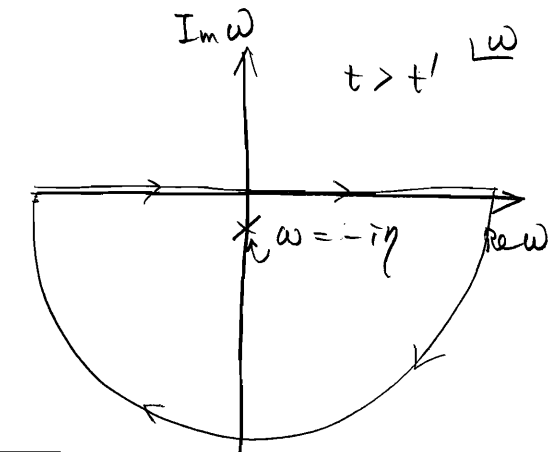
\includegraphics[width = 7cm]{P171.png}
\end{center}
Since the contour encompasses a pole at $\omega=-\mathrm{i}\eta$ in the clockwise way, the integral gives $-2\pi\mathrm{i}$ when $t<t'$, we can put a contour in the upper-half $\omega$-plane, so that the integral here vanishes in the limit of large $|\omega|$, This contour integral doesn't encompass any pole, so that the integral fives zero.

%pic at P172
\begin{center}
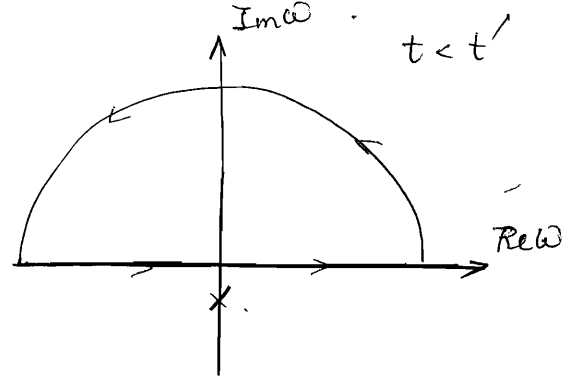
\includegraphics[width = 8cm]{P172.png}
\end{center}
Using this integral representation, the non-interacting fermion green's function can be further calculated as.  
\begin{align}\label{2.3.6}
G^0_{\alpha\beta}(x,t;x',t')&=\frac{1}{2\pi V}\sum_k \int_{-\infty}^{\infty} \mathrm{d}\omega e^{\mathrm{i}k(x-x')-\mathrm{i}\omega_{k}(t-t')} \nonumber \\
& \times \delta_{\alpha\beta}[\frac{\theta(|k|-k_F)}{\omega-\omega_k+\mathrm{i}\eta}+\frac{\theta(k_F-|k|)}{\omega-\omega_k-\mathrm{i}\eta}] \nonumber \\
&\equiv \frac{1}{2\pi V}\sum_k \int_{-\infty}^{\infty}\mathrm{d}\omega e^{\mathrm{i}k(x-x')-\mathrm{i}\omega_{k}(t-t')} G_{\alpha\beta}(k,\omega) \nonumber \\
G_{\alpha\beta}(k,\omega)&\equiv \delta_{\alpha\beta}[\frac{\theta(|k|-k_F)}{\omega-\omega_k+\mathrm{i}\eta}+\frac{\theta(k_F-|k|)}{\omega-\omega_k-\mathrm{i}\eta}] 
\end{align}

To demonstrate how the green's function gives information about the excitation spectrum of the system, let us insert a complete set of eigenstates of H between the two field operators.
\begin{align}\label{2.3.7}
\mathrm{i}G^0_{\alpha\beta}(x,t;x',t')&=\frac{\langle\Psi_0|\mathrm{T}[\hat \psi^{
\dagger}_{H,\alpha}(x,t)\hat \psi_{H,\beta} (x',t')]|\Psi_0\rangle}{\langle\Psi_0|\Psi_0\rangle} \nonumber \\
&=\theta(t-t')\langle\Psi_0|\hat \psi_{H,\alpha}(x,t)\hat{I}\hat \psi^{
\dagger}_{H,\beta} (x',t')|\Psi_0\rangle \nonumber \\
& \ \ \ -\theta(t'-t)\langle\Psi_0|\hat \psi^{
\dagger}_{H,\beta}(x',t')\hat{I}\hat \psi_{H,\alpha} (x,t)|\Psi_0\rangle \nonumber \\
&=\sum_n\{\theta(t-t')\langle\Psi_0|\hat \psi_{H,\alpha}(x,t)|\Psi_n\rangle\times\langle\Psi_n|\hat \psi^{
\dagger}_{H,\beta} (x',t')|\Psi_0\rangle \nonumber \\
& \ \ \ -\theta(t'-t)\langle\Psi_0|\hat \psi^{
\dagger}_{H,\beta}(x',t')|\Psi_n\rangle\times\langle\Psi_n|\hat \psi_{H,\alpha} (x,t)|\Psi_0\rangle\}
\end{align}

Here we assume that the g.s. wave function $|\Psi_0\rangle$ is normalized. And we consider only fermions for simplicity.

By making the time dependence explicit, we can further calculate this as follows

\begin{align}
&=\sum_n\{\theta(t-t')e^{-\mathrm{i}(E_n-E)(t)/\hbar}\langle\Psi_0|\hat \psi_{\alpha}(x)|\Psi_n\rangle\times\langle\Psi_n|\hat \psi^{
\dagger}_{\beta} (x')|\Psi_0\rangle \nonumber \\
& \ \ \ -\theta(t'-t)e^{\mathrm{i}(E_n-E)(t-t')/\hbar}\langle\Psi_0|\hat \psi^{
\dagger}_{\beta}(x')|\Psi_n\rangle\times\langle\Psi_n|\hat \psi_{\alpha} (x)|\Psi_0\rangle\} \nonumber
\end{align}
Note that the states $|\Psi_n\rangle$ here contains N+1 particles if $|\Psi_0\rangle$ contain N particles, while $|\Psi_n\rangle$ here contain N-1 particles.

Now let us assume that the system considered has a translational invariance.

The translational invariance means that the Hamiltonian commute with the total momentum operator $\hat{P}$
\begin{equation}
[\hat{H},\hat{P}]=0\label{2.3.8}
\end{equation}
Where the total momentum operator $\hat{P}$ was already defined in eq(1.4.11) with boson case. But, at this time they are fermion fields.
\begin{equation}
\hat{P}\equiv \sum_{k,\lambda} \hbar k a^k_{k,\lambda} a_{k,\lambda} \nonumber
\end{equation}

Irrespective of this difference, this operator is a generator of the translation.
\begin{equation}\label{2.3.9}
\psi_{\alpha}(x+y)=e^{-\mathrm{i}\hat{P}\cdot y/\hbar}\psi_{\alpha}(x)e^{\mathrm{i}\hat{P}\cdot y/\hbar}
\end{equation}
which can be shown in the same way as we did in eq.(1.4.11).

The translational invariance of the Hamiltonian means that 
\begin{equation}\label{2.3.10}
e^{-\mathrm{i}\hat{P}\cdot y/\hbar}\hat{H}e^{\mathrm{i}\hat{P}\cdot y/\hbar}=\hat{H}
\end{equation}
for any y.

When we use eq.\ref{2.3.3} for $\hat{H}$, this identity means.

\begin{align}
&\sum_{\alpha}\int \mathrm{d}^3x \hat{\psi^{\dagger}_{\alpha}}(x+y)T(x)\hat{\psi_{\alpha}}(x+y)\nonumber \\
&+\frac{1}{2}\sum_{\alpha,\alpha',\beta,\beta'}\int\mathrm{d}^3x\int\mathrm{d}^3x'\psi^{\dagger}_{\alpha}(x+y)\psi^{\dagger}_{\beta}(x'+y)V_{\alpha\alpha',\beta\beta'}(x,x')\psi^{\dagger}_{\beta'}(x'+y)\psi^{\dagger}_{\alpha}(x+y) \nonumber \\
&=\sum_{\alpha}\int \mathrm{d}^3x \hat{\psi^{\dagger}_{\alpha}}(x)T(x)\hat{\psi_{\alpha}}(x)\nonumber \\
&+\frac{1}{2}\sum_{\alpha,\alpha',\beta,\beta'}\int\mathrm{d}^3x\int\mathrm{d}^3x'\psi^{\dagger}_{\alpha}(x)\psi^{\dagger}_{\beta}(x')V_{\alpha\alpha',\beta\beta'}(x,x')\psi^{\dagger}_{\beta'}(x')\psi^{\dagger}_{\alpha}(x) \nonumber
\end{align}
which clearly represents the translation invariance of the system.

When expanding eq.\ref{2.3.10} in y, we have, 
\begin{equation}
\hat{H}-\mathrm{i}\frac{1}{\hbar}[\hat{P}\cdot y,\hat{H}]+O(y^2)=\hat{H} \nonumber
\end{equation}
for any y.

which gives us eq.\ref{2.3.8}

Now that the Hamiltonian commute with the total momentum operator, any eigenstate of $\hat{H}$ should be also eigenstate of $\hat{P}$.

\begin{equation}\label{2.3.11}
\hat{P}|\Psi_n\rangle=P_n|\Psi_n\rangle
\end{equation}

Then, using eq.\ref{2.3.9} \& eq.\ref{2.3.11}, we can also extract the x-dependence of eq.\ref{2.3.7}
\begin{align}
&\mathrm{i}G^0_{\alpha\beta}(x,t;x',t') \nonumber \\
&=\sum_n\bigg [\theta(t-t')e^{-\mathrm{i}(E_n-E)(t)/\hbar}e^{\mathrm{i}\hat{P_n}(x-x')/\hbar}\langle\Psi_0|\hat \psi_{\alpha}(0)|\Psi_n\rangle\times\langle\Psi_n|\hat \psi^{
\dagger}_{\beta} (0)|\Psi_0\rangle \nonumber \\
& \ \ \ -\theta(t'-t)e^{\mathrm{i}(E_n-E)(t-t')/\hbar}e^{-\mathrm{i}\hat{P_n}(x-x')}\langle\Psi_0|\hat \psi^{
\dagger}_{\beta}(0)|\Psi_n\rangle\times\langle\Psi_n|\hat \psi_{\alpha} (0)|\Psi_0\rangle \bigg ] \nonumber
\end{align}
Here we assume that the ground state wave function has zero total momentum.

\begin{equation}
\hat{P}|\Psi_0\rangle=0 \nonumber
\end{equation}
which is usually the case.

Then the Fourier transform of the green's function is given by
\begin{align}
G_{\alpha\beta}(k,\omega)&\equiv\int \mathrm{d}^3(x-x')\int \mathrm{d}^3(t-t')e^{-\mathrm{i}k(x-x')+\mathrm{i}\omega(t-t')}G_{\alpha\beta}(x,t;x',t') \nonumber \\
&=V\sum_n \delta_{k,\hat P_n/\hbar} \frac{\langle\Psi_0|\hat \psi_{\alpha}(0)|\Psi_n\rangle\times\langle\Psi_n|\hat \psi^{
\dagger}_{\beta} (0)|\Psi_0\rangle}{\omega-(E_n-E)/\hbar +\mathrm{i}\eta}  \nonumber \\
&+V\sum_n \delta_{k,-\hat P_n/\hbar} \frac{\langle\Psi_0|\hat \psi^{
\dagger}_{\beta} (0)|\Psi_n\rangle\times\langle\Psi_n|\hat \psi_{\alpha}(0)|\Psi_0\rangle}{\omega+(E_n-E)/\hbar -\mathrm{i}\eta}  \nonumber
\end{align}

This restricts the state $|\Psi_n\rangle$ to have a wave number k, so that we can rewrite this as
\begin{align}
& G_{\alpha\beta}(k,\omega) \nonumber \\
&=V\sum_n \delta_{k,\hat P_n/\hbar} \frac{\langle\Psi_0|\hat \psi_{\alpha}(0)|n,k\rangle\langle n,k|\hat \psi^{
\dagger}_{\beta} (0)|\Psi_0\rangle}{\omega-(E_n-E)/\hbar +\mathrm{i}\eta}  \nonumber \\
&+V\sum_n \delta_{k,-\hat P_n/\hbar} \frac{\langle\Psi_0|\hat \psi^{
\dagger}_{\beta} (0)|n,-k\rangle\langle n,-k|\hat \psi_{\alpha}(0)|\Psi_0\rangle}{\omega+(E_n-E)/\hbar -\mathrm{i}\eta}  \nonumber
\end{align}

In the first sum, the intermediate state has N+1 particles, so that the denominator can be rewritten as
\begin{align}
\omega-[E_n(N+1)-E(N)]/\hbar &= \omega-[E_n(N+1)-E(N+1)]/\hbar-[E(N+1)-E(N)]/\hbar \nonumber \\
&=\omega-\mu/\hbar-\epsilon_n(N+1)/\hbar \nonumber
\end{align}
where $E(N+1)$ and $\epsilon_n(N+1)$ are the ground and the excitation state energy of the (N+1) particle state.

Similarly, the denominator of the second term can be rewritten as 
\begin{align}
\omega+[E_n(N-1)-E(N)]/\hbar &= \omega+[E_n(N-1)-E(N-1)]/\hbar-[E(N)-E(N-1)]/\hbar \nonumber \\
&=\omega-\mu/\hbar+\epsilon_n(N-1)/\hbar \nonumber
\end{align}

Where, in the thermodynamics limit the difference between the former chemical potential and the latter one is negligible.
\begin{align}
E(N+1)-E(N)-(E(n)-E(n-1))=O(N^{-1}) \nonumber \\
\bigg ( Ve(n+\frac{1}{V}) = Ve(n)+ V\frac{\partial e}{\partial n}\frac{1}{V} + \frac{1}{2} \frac{\partial^2 e}{\partial n^2} (\frac{1}{V})^2 \bigg) \nonumber
\end{align}

Using these two, we now obtain 
\begin{align}\label{2.3.12}
& G_{\alpha\beta}(k,\omega) \nonumber \\
&=\hbar V\sum_n \frac{\langle\Psi_0|\hat \psi_{\alpha}(0)|n,k\rangle\langle n,k|\hat \psi^{
\dagger}_{\beta} (0)|\Psi_0\rangle}{\omega\hbar-\mu-\epsilon_n(N+1)+\mathrm{i}\eta}  \nonumber \\
&+\hbar V\sum_n \frac{\langle\Psi_0|\hat \psi^{
\dagger}_{\beta} (0)|n,-k\rangle\langle n,-k|\hat \psi_{\alpha}(0)|\Psi_0\rangle}{\omega\hbar-\mu+\epsilon_n(N-1)-\mathrm{i}\eta} 
\end{align}

This representation of single-particle green's function is called as Lehmann representation.

If the Hamiltonian and the ground state are invariant under the spatial rotation and reflection, the green's function has a following matrix structure.
\begin{equation}
G_{\alpha\beta}=\delta_{\alpha\beta}G(|k|,\omega) \nonumber
\end{equation}

The lehmann rep. exhibits the $\omega$-dependence of the exact green's function of interacting systems.

The function $G(k,\omega)$ is a meromorphic function of $\omega$, with simple poles at the exact excitation energy of the interacting system corresponding to a momentum $\hbar k$.

For frequencies below $\mu/\hbar$, these singularities lies slightly above the real axis and for frequencies above $\mu/\hbar$, these singularities  lies slightly below the real axis.

%pic at P184
\begin{center}
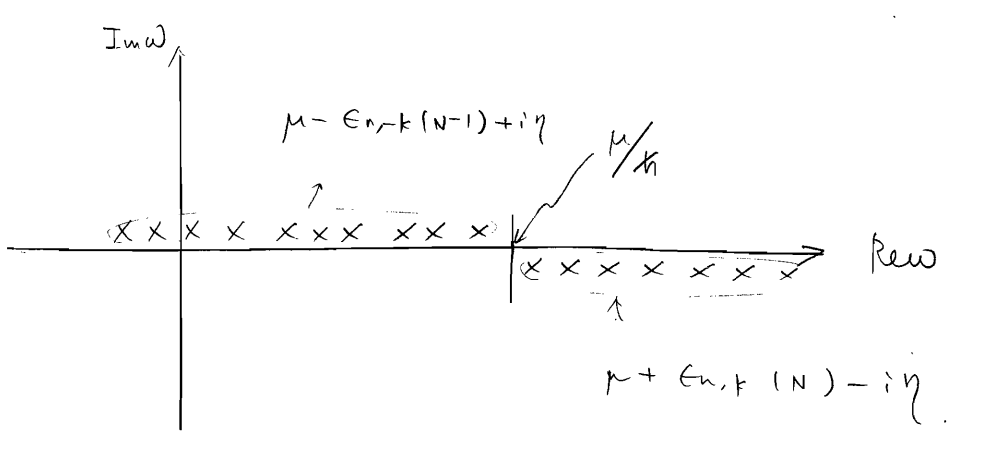
\includegraphics[width = 10cm]{P184.png}
\end{center}
In this way, the singularities if the green's function yield the energies of those excited states for which the numerator ($\langle n,k|\hat \psi^{
\dagger}_{\beta} (0)|\Psi_0\rangle$ or $\langle n,-k|\hat \psi_{\alpha}(0)|\Psi_0\rangle$) does not vanish. 

For the non-interacting system, this representation ?? reproduce eq.\ref{2.3.6}.

\begin{equation}
G^0(k,\omega)=\frac{\theta(k-k_F)}{\omega-\omega_k+\mathrm{i}\eta}+\frac{\theta(k_F-k)}{\omega-\omega_k-\mathrm{i}\eta} \nonumber
\end{equation} 
with $\omega_k=\frac{\hbar^2k^2}{2m}$

Namely, for the non-interacting system, the field operator connects only one state to the ground state, so that $G^0(k,\omega)$ has only a single pole, slightly below the real axis at $\hbar \omega=\frac{\hbar^2k^2}{2m}$ if $k>k_F$ and slightly above the real axis at the same value of $\hbar \omega$ of $k<k_F$.


% pic at P185
\begin{center}
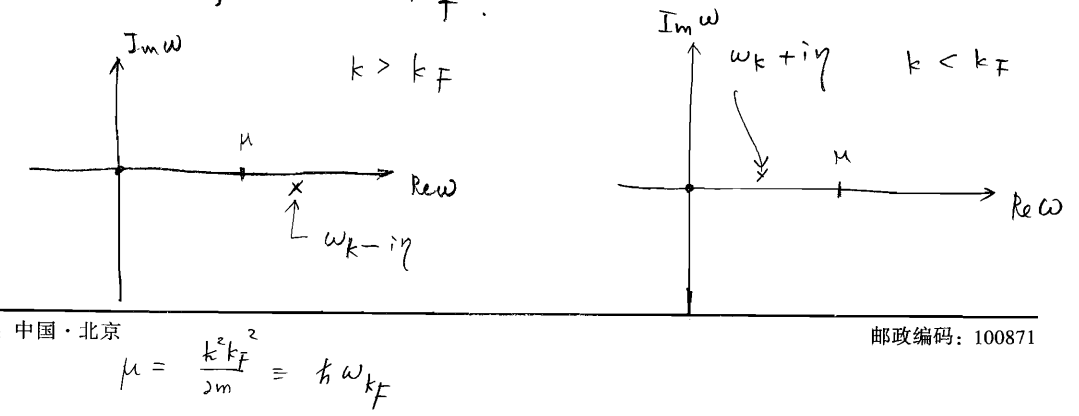
\includegraphics[width = 12cm]{P185.png}
\end{center}

The green's function is analytic in neither the upper $\omega$-plane nor the lower $\omega$-plane.

We define a new pair of function, known as retard and advance green's functions.
\begin{align}\label{2.3.13}
\mathrm{i}G^R_{\alpha\beta}(x,t;x',t')=\langle \Psi_0|\{\hat \psi_{H,\alpha}(x,t),\psi^{\dagger}_{H,\beta}(x',t')\}|\Psi_0\rangle\theta(t-t')
\end{align}
\begin{align}\label{2.3.14}
\mathrm{i}G^A_{\alpha\beta}(x,t;x',t')=\langle \Psi_0|\{\hat \psi_{H,\alpha}(x,t),\psi^{\dagger}_{H,\beta}(x',t')\}|\Psi_0\rangle\theta(t'-t)
\end{align}
with $\{A,B\}\equiv AB+BA$

Using the exactly same analysis, we can show the following Lehmann representation of their Fourier transforms.

\begin{align}\label{2.3.15}
& G^{R/A}_{\alpha\beta}(k,\omega) \nonumber \\
&=\hbar V\sum_n \frac{\langle\Psi_0|\hat \psi_{\alpha}(0)|n,k\rangle\langle n,k|\hat \psi^{
\dagger}_{\beta} (0)|\Psi_0\rangle}{\omega\hbar-\mu-\epsilon_n(N+1)\pm\mathrm{i}\eta}  \nonumber \\
&+\hbar V\sum_n \frac{\langle\Psi_0|\hat \psi^{
\dagger}_{\beta} (0)|n,-k\rangle\langle n,-k|\hat \psi_{\alpha}(0)|\Psi_0\rangle}{\omega\hbar-\mu+\epsilon_n(N-1)\pm\mathrm{i}\eta} \nonumber\tag{2.3.15A/B} 
\end{align}

Note that all the poles of $G^R$ lie in the lower half plane, so that $G^A(k,\omega)$ is analytic for $\mathrm{Im} \omega<0$



\section{Wick's theorem}

So far, we define the single-particle green's function and show its relation to physical observables.

To evaluate the green's function for nontrivial physical systems, we use perturbation theory.

This procedure is mostly carried out in the interacting picture, instead of the Heinsenberg picture.

Let me first prove a basic Theorem that relates the matrix elements of Heisenberg operators to the matrix elements of the corresponding interaction operators.


\begin{align}\label{2.4.1}
\frac{\langle\Psi_0|\hat{O_H}(t)|\Psi_0\rangle}{\langle\Psi_0|\Psi_0\rangle}=\frac{1}{\langle\Phi_0|\hat{S}|\Phi_0\rangle}\times \langle\Phi_0|\sum_{\nu=0}^{\infty}(\frac{-\mathrm{i}}{\hbar})^{\nu} \frac{1}{\nu!} \int_{-\infty}^{+\infty}\mathrm{d}t_1......\int_{-\infty}^{+\infty}\mathrm{d}t_{\nu} \nonumber \\
e^{-\epsilon(|t_1|+...+|t_{\nu}|)}\mathrm{T}[\hat{H_1}(t_1)...\hat{H_1}(t_{\nu})]\hat{O_I}(t)|\Phi_0\rangle
\end{align}
where 
\begin{equation}\label{2.4.2}
\hat{S}\equiv\hat{U_{\epsilon}}(\infty,-\infty)
\end{equation}

The proof is as follows.

According to the Gell-Mann \& Low Theorem, $|\Psi_0\rangle$ can be given by

\begin{align}
\frac{|\Psi_0\rangle}{\langle\Phi_0|\Psi_0\rangle}&=\frac{\hat{U_{\epsilon}}(+\infty,0)|\Psi_0\rangle}{\langle\Phi_0|\hat U_{\epsilon}(+\infty,0)|\Psi_0\rangle} \nonumber \\
&=\frac{\hat{U_{\epsilon}}(0,-\infty)|\Psi_0\rangle}{\langle\Phi_0|\hat U_{\epsilon}(0,-\infty)|\Psi_0\rangle} \nonumber
\end{align}

By taking an inner product between these two, we can calculate this part
\begin{align}
\frac{\langle\Psi_0|\Psi_0\rangle}{|\langle\Phi_0|\Psi_0\rangle|^2}&=\frac{\langle\Phi_0|\hat{U_{\epsilon}}(+\infty,0)\hat{U_{\epsilon}}(0,-\infty)|\Phi_0\rangle}{\langle\Phi_0|\hat{U^{\dagger}_{\epsilon}}(+\infty,0)|\Phi_0\rangle^*\langle\Phi_0|\hat{U_{\epsilon}}(0,-\infty)|\Phi_0\rangle} \nonumber \\
&=\frac{\langle\Phi_0|\hat{U_{\epsilon}}(+\infty,0)\hat{U_{\epsilon}}(0,-\infty)|\Phi_0\rangle}{D} \nonumber \\
&= \frac{\langle\Phi_0|\hat{U_{\epsilon}}(+\infty,-\infty)|\Phi_0\rangle}{D} \nonumber
\end{align}
The numerator can be also calculated in a similar way.
\begin{align}
\frac{\langle\Psi_0|\hat{O_H}(t)|\Psi_0\rangle}{|\langle\Phi_0|\Psi_0\rangle|^2}&=\frac{\langle\Phi_0|\hat{U_{\epsilon}}(+\infty,0)\hat{O_H}(t)\hat{U_{\epsilon}}(0,-\infty)|\Phi_0\rangle}{\langle\Phi_0|\hat{U^{\dagger}_{\epsilon}}(+\infty,0)|\Phi_0\rangle^*\langle\Phi_0|\hat{U_{\epsilon}}(0,-\infty)|\Phi_0\rangle} \nonumber \\
&=\frac{\langle\Phi_0|\hat{U_{\epsilon}}(+\infty,0)\hat{U_{\epsilon}}(0,t)\hat{O_I}(t)\hat{U_{\epsilon}}(t,0)\hat{U_{\epsilon}}(0,-\infty)|\Phi_0\rangle}{D} \nonumber \\
&=\frac{\langle\Phi_0|\hat{U_{\epsilon}}(+\infty,t)\hat{O_I}(t)\hat{U_{\epsilon}}(t,-\infty)|\Phi_0\rangle}{D} \nonumber
\end{align}


Now that these two equations share the same denominator, we can make them cancel each other so as to obtain
\begin{align}
\frac{\langle\Psi_0|\hat{O_H}(t)|\Psi_0\rangle}{\langle\Psi_0|\Psi_0\rangle}=\frac{\langle\Phi_0|\hat{U_{\epsilon}}(+\infty,t)\hat{O_I}(t)\hat{U_{\epsilon}}(t,-\infty)|\Phi_0\rangle}{\langle\Phi_0|\hat{U_{\epsilon}}(+\infty,-\infty)|\Phi_0\rangle}\nonumber
\end{align}

The numerator  of the r.h.s is given as
\begin{align}
\hat{U_{\epsilon}}(+\infty,t)\hat{O_I}(t)\hat{U_{\epsilon}}(t,-\infty)=&\sum_{n=0}^{\infty}(\frac{-\mathrm{i}}{\hbar})^{n} \frac{1}{n!} \int_{-\infty}^{+\infty}\mathrm{d}t_1......\int_{-\infty}^{+\infty}\mathrm{d}t_{n} \nonumber \\
& \times e^{-\epsilon(|t_1|+...+|t_{n}|)}\mathrm{T}[\hat{H_1}(t_1)...\hat{H_1}(t_{n})]\hat{O_I}(t)\times \nonumber \\
& \sum_{m=0}^{\infty}(\frac{-\mathrm{i}}{\hbar})^{m} \frac{1}{m!} \int_{-\infty}^{+\infty}\mathrm{d}s_1......\int_{-\infty}^{+\infty}\mathrm{d}s_{m} \nonumber \\
& \times e^{-\epsilon(|s_1|+...+|s_{m}|)}\mathrm{T}[\hat{H_1}(s_1)...\hat{H_1}(s_{m})]\times \nonumber \\
& ...... \nonumber
\end{align}

On the one hand, the numerator of eq.\ref{2.4.1} can be rewritten as follows.

Firstly, suppose that we divide  $\nu$-numbers of $\hat{H_1}$ into n-numbers of $\hat{H_1}$ whose times one greater than 't' and ($\nu$-n)-numbers of $\hat{H_1}$ whose times are less than 't',
\begin{align}
=\sum_{\nu=0}^{\infty}(\frac{-\mathrm{i}}{\hbar})^{\nu} \frac{1}{\nu!} \sum_{n=0}^{\nu}\frac{\nu!}{n!(\nu-n)!}e^{-\epsilon(|t_1|+...+|t_{\nu}|)} \int_{t}^{+\infty}\mathrm{d}t_1...\int_{t}^{+\infty}\mathrm{d}t_{n} 
\int_{-\infty}^{t}\mathrm{d}t_{n+1}...\int_{-\infty}^{t}\mathrm{d}t_{\nu} \nonumber \\
\mathrm{T}[\hat{H_1}(t_1)...\hat{H_1}(t_{n})]\hat{O_I}(t)\mathrm{T}[\hat{H_1}(t_{n+1})...\hat{H_1}(t_{\nu})] \nonumber
\end{align}

There is $\frac{\nu!}{n!(\nu-n)!}$ number of (the factorial of $\nu$ divided by the factorial of n times the factorial of ($\nu-n$)) ways of dividing.

Thus, once we choose $t_1,t_2,...,t_n$ to be greater than t while the  remaining to be less than t, we need to multiply this factor.

Since 
\begin{equation}
\sum_{\nu=0}^{+\infty}\sum_{n=0}^{\nu} f_{n,\nu}=\sum_{m=0}^{+\infty}\sum_{n=0}^{\nu} f_{n,m+n} \nonumber
\end{equation}
%pic at194
\begin{center}
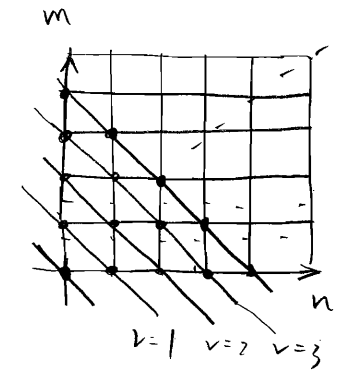
\includegraphics[width = 4cm]{P194.png}
\end{center}
So that
\begin{align}
=&\sum_{m=0}^{+\infty}\frac{1}{m!}(\frac{-\mathrm{i}}{\hbar})^m\sum_{n=0}^{+\infty} \frac{1}{n!}(\frac{-\mathrm{i}}{\hbar})^ne^{-\epsilon(|t_1|+...+|t_{m+n}|)} \nonumber \\
&\int_{t}^{+\infty}\mathrm{d}t_1...\int_{t}^{+\infty}\mathrm{d}t_n\int_{-\infty}^{t}\mathrm{d}t_{n+1}...\int_{-\infty}^{t}\mathrm{d}t_{n+m} \nonumber \\
&\mathrm{T}[\hat{H_1}(t_1)...\hat{H_1}(t_n)]\hat{O_I}(t)\mathrm{T}[\hat{H_1}(t_{n+1})...\hat{H_1}(t_{n+m})] \nonumber \\
=& \hat U_{\epsilon}(-\infty,t)\hat{O_I}(t)\hat U_{\epsilon}(t,-\infty) \nonumber
\end{align}

This proves eq.\ref{2.4.1}

In a similar way, we can show that  the expectation value of time-ordered Heinsenberg operator can be expressed in terms of the interaction picture.
\begin{align}\label{2.4.3}
\frac{\langle\Psi_0|\mathrm{T}[\hat{O_H}(t)\hat{O_H}(t')]|\Psi_0\rangle}{\langle\Psi_0|\Psi_0\rangle}=&\frac{1}{\langle\Phi_0|\hat{S}|\Phi_0\rangle}\times\langle\Phi_0|\sum_{\nu=0}^{\infty}(\frac{-\mathrm{i}}{\hbar})^{\nu} \frac{1}{\nu!} \int_{-\infty}^{+\infty}\mathrm{d}t_1......\int_{-\infty}^{+\infty}\mathrm{d}t_{\nu}e^{-\epsilon(|t_1|+...+|t_{\nu}|)} \nonumber\\
&\times \mathrm{T}[\hat{H_1}(t_1)...\hat{H_1}(t_{\nu})\hat{O_I}(t)\hat{O_I}(t')]|\Phi_0\rangle
\end{align}
The r.h.s reads.
\begin{align}
&\frac{\langle\Psi_0|\mathrm{T}[\hat O_{H}(t)\hat O_H (t')]|\Psi_0\rangle}{\langle\Psi_0|\Psi_0\rangle} \nonumber \\
=&\theta(t-t')\langle\Psi_0|\hat O_{H}(t)\hat O_H (t')|\Psi_0\rangle \nonumber \\
& \ \ +\theta(t'-t)\langle\Psi_0|\hat O_{H}(t')\hat O_H (t)|\Psi_0\rangle \nonumber 
\end{align}
The numerator of the first term can be calculated in the same way as before,
\begin{align}
\frac{\langle\Psi_0|\hat{O_H}(t)\hat{O_H}(t')|\Psi_0\rangle}{|\langle\Phi_0|\Psi_0\rangle|^2}&=\frac{\langle\Phi_0|\hat{U_{\epsilon}}(+\infty,0)\hat{O_H}(t)\hat{O_H}(t')\hat{U_{\epsilon}}(0,-\infty)|\Phi_0\rangle}{D} \nonumber \\
&=\frac{\langle\Phi_0|\hat{U_{\epsilon}}(+\infty,t)\hat{O_I}(t)\hat{U_{\epsilon}}(t,t')\hat{O_I}(t')\hat{U_{\epsilon}}(t',-\infty)|\Phi_0\rangle}{D} \nonumber
\end{align}
So that, we can employ the same cancellation between D which comes from the numerator and D which comes from the denominator.
\begin{align}
\frac{\langle\Psi_0|\hat{O_H}(t)\hat{O_H}(t')|\Psi_0\rangle}{\langle\Psi_0|\Psi_0\rangle}=\frac{\langle\Phi_0|\hat{U_{\epsilon}}(+\infty,t)\hat{O_I}(t)\hat{U_{\epsilon}}(t,t')\hat{O_I}(t')\hat{U_{\epsilon}}(t',-\infty)|\Phi_0\rangle}{\langle\Phi_0|\hat{U_{\epsilon}}(+\infty,-\infty)|\Phi_0\rangle}\nonumber
\end{align}
for $t'>t$

On the one hand, the numerator of the r.h.s of eq.\ref{2.4.3} can be calculated as
\begin{align}
(r.h.s)=\theta&(t-t')\langle \Phi_0|\sum_{\nu=0}^{\infty}(\frac{-\mathrm{i}}{\hbar})^{\nu} \frac{1}{\nu!}\sum_{n}\sum_{m}^{0<n+m\le\nu}\frac{\nu!}{n!m!(\nu-n-m)!}\nonumber\\ &\int_{t}^{+\infty}\mathrm{d}t_1...\int_{t}^{+\infty}\mathrm{d}t_{n}\int_{t'}^{t}\mathrm{d}t_{n+1}...\int_{t'}^{t}\mathrm{d}t_{n+m}\int_{-\infty}^{t'}\mathrm{d}t_{n+m+1}...\int_{-\infty}^{t'}\mathrm{d}t_{\nu} \nonumber \\
\times&  \mathrm{T}[\hat{H_1}(t_1)...\hat{H_1}(t_{n})]\hat{O_I}(t)\mathrm{T}[\hat{H_1}(t_{n+1})...\hat{H_1}(t_{n+m})]\hat{O_I}(t')\mathrm{T}[\hat{H_1}(t_{n+m+1})...\hat{H_1}(t_{\nu})]|\Phi_0\rangle \nonumber \\
+&\theta(t'-t)\langle \Phi_0|\sum_{\nu=0}^{\infty}(\frac{-\mathrm{i}}{\hbar})^{\nu} \frac{1}{\nu!}\sum_{n}\sum_{m}^{0\le n+m\le\nu}\frac{\nu!}{n!m!(\nu-n-m)!}\nonumber\\ &\int_{t'}^{+\infty}\mathrm{d}t_1...\int_{t'}^{+\infty}\mathrm{d}t_{n}\int_{t}^{t'}\mathrm{d}t_{n+1}...\int_{t}^{t'}\mathrm{d}t_{n+m}\int_{-\infty}^{t}\mathrm{d}t_{n+m+1}...\int_{-\infty}^{t}\mathrm{d}t_{\nu} \nonumber \\
\times&  \mathrm{T}[\hat{H_1}(t_1)...\hat{H_1}(t_{n})]\hat{O_I}(t')\mathrm{T}[\hat{H_1}(t_{n+1})...\hat{H_1}(t_{n+m})]\hat{O_I}(t)\mathrm{T}[\hat{H_1}(t_{n+m+1})...\hat{H_1}(t_{\nu})]|\Phi_0\rangle \nonumber
\end{align}
This part can be replaced by this
\begin{align}
&\sum_{\nu=0}^{\infty}\sum_{n}\sum_{m}^{0<n+m\le\nu}\frac{1}{n!m!(\nu-n-m)!}\nonumber\\
=&\sum_{n=0}^{\infty}\sum_{m=0}^{\infty}\sum_{l=0}^{\infty}\frac{1}{n!m!l!} \nonumber
\end{align}
%pic at199
\begin{center}
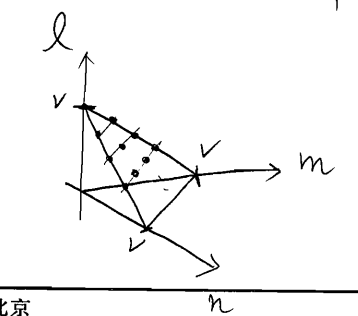
\includegraphics[width = 3cm]{P199.png}
\end{center}
So that the first term reduces to
\begin{align}
(1st \  term)=\theta(t-t')\langle\Phi_0|\hat{U_{\epsilon}}(+\infty,t)\hat{O_I}(t)\hat{U_{\epsilon}}(t,t')\hat{O_I}(t')\hat{U_{\epsilon}}(t',-\infty)|\Phi_0\rangle \nonumber
\end{align}
while the 2nd term reduces to
\begin{align}
(2nd \  term)=\theta(t'-t)\langle\Phi_0|\hat{U_{\epsilon}}(+\infty,t')\hat{O_I}(t')\hat{U_{\epsilon}}(t',t)\hat{O_I}(t)\hat{U_{\epsilon}}(t,-\infty)|\Phi_0\rangle \nonumber
\end{align}
which proves eq.\ref{2.4.3}

These two formula are among the most useful results of quantum field theory.


Armed with these formulas, let us consider the  single-particle green's function, which is now given in the interaction picture.
\begin{align}\label{2.4.4}
\mathrm{i}G_{\alpha\beta}(x,t;x',t')=\sum_{\nu=0}^{\infty}(\frac{-\mathrm{i}}{\hbar})^{\nu} \frac{1}{\nu!} \int_{-\infty}^{+\infty}\mathrm{d}t_1......\int_{-\infty}^{+\infty}\mathrm{d}t_{\nu}\times\nonumber  \\
\frac{\langle\Phi_0|\mathrm{T[\hat H_1(t_1)...\hat H_1(t_{\nu})\hat \Psi_{I,\alpha}(x)\Psi^{\dagger}_{I,\beta}(x')]}
|\Phi_0\rangle}{\langle\Phi_0|\hat{U_{\epsilon}}(+\infty,-\infty)|\Phi_0\rangle}
\end{align}
where $x\ \&\ x'$ here denotes space and temporal coordinate.$x\equiv(x,t),x\equiv (x',t')$
\begin{align}
\Psi_{I,\alpha}(x)&\equiv\Psi_{I,\alpha}(x,t) \nonumber \\
&=e^{\mathrm{i}\hat{H_0}t/\hbar}\Psi_{\alpha}(x)e^{-\mathrm{i}\hat{H_0}t/\hbar} \nonumber
\end{align}
This operator is now creation and annihilation operator in the interaction picture.

For Hamiltonian defined in eq.\ref{2.3.3}, the numerator of this eq. becomes as follows:

numerator of eq.\ref{2.4.4}
\begin{align}\label{2.4.5}
& numerator of eq.\ref{2.4.4} \nonumber \\
=&\langle \Phi_0|\mathrm{T}[\hat \psi_{\alpha }(x)\hat \psi_{\beta }^{\dagger}(x')]|\Phi\rangle \nonumber \\
&+(\frac{-\mathrm{i}}{\hbar})\sum_{\lambda,\lambda',\mu,\mu'}\frac{1}{2}\int_{-\infty}^{+\infty}\mathrm{d}t_1\int\mathrm{d}^3x_1\int\mathrm{d}^3x_1' \nonumber \\
&\times U_{\lambda\lambda',\mu\mu'}(x_1,x_1')\times \nonumber\\
&\Phi_0|\mathrm{T}[\hat \psi_{I,\lambda}^{\dagger}(x_1,t_1)\hat \psi_{I,\mu}^{\dagger}(x_1',t_1)\hat \psi_{I,\mu' }(x_1',t_1) \nonumber \\
&\ \ \ \hat \psi_{I,\lambda' }(x_1,t_1)\hat \psi_{I,\alpha}(x,t)\hat \psi^{\dagger}_{I,\beta }(x',t)]|\Phi\rangle \nonumber \\
&\ \ \ \ \ +......
\end{align}
This expression shows that, we must evaluate the expectation value in the non-interacting ground state of T-products of creation \& destruction operators of the form:
\begin{align}
\Phi_0|\mathrm{T}[\hat \psi_{I}^{\dagger}......\hat \psi_{I}\hat \psi_{I,\alpha}(x)\hat \psi^{\dagger}_{I,\beta }(x')]|\Phi\rangle \nonumber 
\end{align}
To evaluate this form of quantities, we will rely on so-called Wick's theorem, which I will explain next.

The essential ideas of Wick's theorem is to move all destruction operators to the right, where they annihilate the non-interacting ground state wave function.

For this purpose, we decompose the field operator into a destruction part (the 1st term in the r.h.s of following equation) that annihilates the non-interacting ground state and a creation part(the 2nd term).
\begin{align}
\hat \psi_{I}(x)=\hat \psi^{(+)}_{I}(x)&+\hat \psi^{(-)}_{I}(x) \nonumber \\
\hat \psi^{(+)}_{I}(x)|\Phi_0\rangle&=0 \nonumber
\end{align}

Note also that any two pairs of destruction operators thus defined commute or anticommute with each other, which can be seen by taking the expectation value of their commutator or anticommutator.

\begin{align}
&\{\hat \psi^{(+)}(x),\hat \psi^{(+)}(y)\}_{\pm}=0 \nonumber \\
\big (&\leftarrow\langle\Phi_0|\hat \psi^{(+)}(x)\hat \psi^{(+)}(y)\pm\hat \psi^{(+)}(y),\hat \psi^{(+)}(x)|\Phi_0\rangle \big) \nonumber \\
&\{\hat \psi^{(-)\dagger}(x),\hat \psi^{(+)}(y)\}_{\pm}=0 \nonumber \\
\big (&\leftarrow\langle\Phi_0|\hat \psi^{(-)\dagger}(x)\hat \psi^{(+)}(y)\pm\hat \psi^{(+)}(y),\hat \psi^{(-)\dagger}(x)|\Phi_0\rangle \big) \nonumber
\end{align} 
+ for fermion case, - for boson case.

Similarly, we can see that any two pairs of creation part commute of anticommute with each other.
\begin{align}
&\{\hat \psi^{(-)}(x),\hat \psi^{(-)}(y)\}_{\pm}=\{\hat \psi^{(-)}(x),\hat \psi^{(+)\dagger}(y)\}_{\pm} \nonumber \\
=&\{\hat \psi^{(+)\dagger}(x),\hat \psi^{(+)\dagger}(y)\}_{\pm}=0 \nonumber 
\end{align}

Correspondingly, we have
\begin{align}
\hat \psi^{\dagger}_{I}(x)=\hat \psi^{(+)\dagger}_{I}(x)&+\hat \psi^{(-)\dagger}_{I}(x) \nonumber \\
\hat \psi^{(-)}_{I}(x)|\Phi_0\rangle&=0 \nonumber
\end{align}
Where we take the adjoint of this, so as to obtain this.?

As an explicit example of this decomposition, consider the free fermion field given in eq.??
\begin{align}
\hat \psi_I(x)=\frac{1}{\sqrt{V}}\sum_{k>k_F} e^{\mathrm{i}(kx-\mathrm{i}\omega_kt)}a_k+\frac{1}{\sqrt{V}}\sum_{k<k_F} e^{\mathrm{i}(kx-\mathrm{i}\omega_kt)}a_k \nonumber
\end{align}
Where I have omitted the spin index

This satisfies $\hat \phi^{(-)}(x)|\Phi_0\rangle=\hat \phi ^{(+)}|\Phi_0\rangle=0$, because $|\Phi_0\rangle$ is a Fermi sea state with fermions being occupied up to the fermi level.

$\circledcirc$ As was already defined in eq\ref{2.3.2}, time-order products orders the field operators with the latest time om the left
\begin{align}
\mathrm{T}(\hat{A}\hat{B}\hat{C}\hat{D}...)=(-1)^P\hat{B}\hat{D}\hat{C}\hat{A}... \nonumber
\end{align}
with $t_B>t_D>t_C>t_A>...$

Where this factor become +1 if the time ordering is accompanied by the even numbers of interchange of the fermion field.

while this factor become -1 if the time ordering is accompanied by the odd numbers of interchange of the fermion field.

For boson case, this is always +1.

Thus, we can freely reorder the field operators within the F product, in such a way that fermion fields anticommute and boson fields commute.

$\circledcirc$ The other important operator product is the "normal ordering", in which all the annihilation operators are placed to the right of all the creation operators again including a factor -1 for every interchange of fermion operators.
 % pic at P209
 \begin{center}
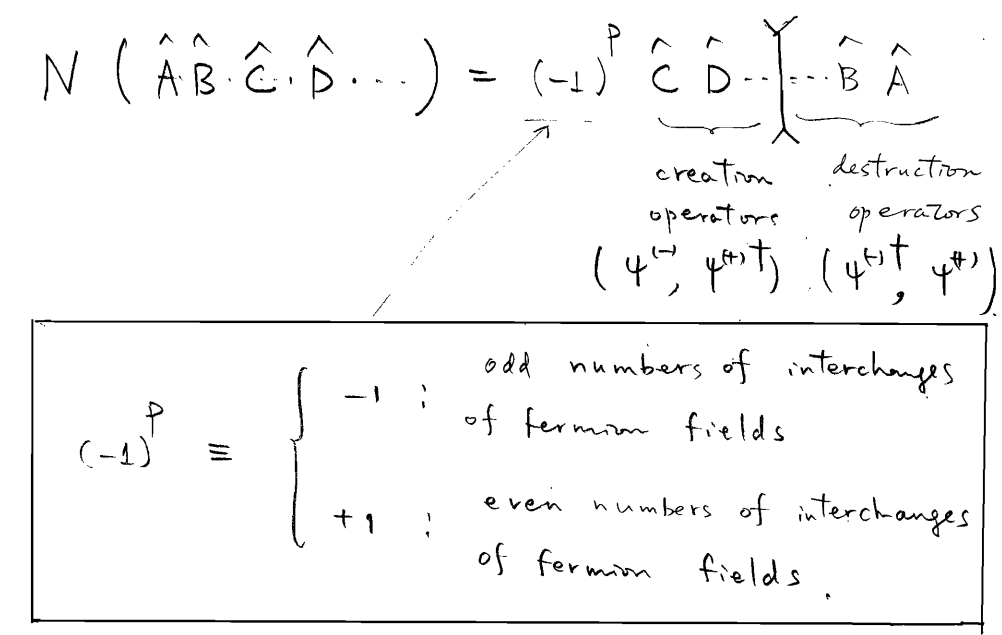
\includegraphics[width = 12cm]{P209.png}
\end{center}
Here the destruction operators means a destruction part of field operator which annihilates the non-interacting groundstate. while the creation operator means a creation part which does not.

Because any two pairs of destruction parts commute or anticommute with each other and also because that is the case for creation parts, the r.h.s of this is uniquely defined.

Namely, a specific order within a set of destruction operators in the right and that with a set of creation operators in the left don't make any difference.

For example, for fermion case, we have 

\begin{align}
\mathrm{N}[\hat \psi^{(+)}(x)\hat \psi^{(-)}(y)]&=-\hat \psi^{(-)}(y)\hat \psi^{(+)}(x) \nonumber \\
\mathrm{N}[\hat \psi^{(-)\dagger}(x)\hat \psi^{(+)\dagger}(y)]&=-\hat \psi^{(+)\dagger}(y)\hat \psi^{(-)\dagger}(x) \nonumber \\
\mathrm{N}[\hat \psi^{(-)\dagger}(x)\hat \psi^{(+)}(y)]&=\hat \psi^{(-)\dagger}(x)\hat \psi^{(+)}(y) \nonumber \\
&=-\hat \psi^{(+)}(y)\hat \psi^{(-)\dagger}(x) \nonumber \\
\mathrm{N}[\hat \psi^{(-)}(x)\hat \psi^{(+)\dagger}(y)]&=\hat \psi^{(-)}(x)\hat \psi^{(+)\dagger}(y) \nonumber \\
&=-\hat \psi^{(+)\dagger}(y)\hat \psi^{(-)}(x) \nonumber 
\end{align}
Here I have omitted the subscript 'I'. I will do so in the remaining part of today's lecture, because the field operators are always in the interaction picture.

A normal order product is very useful, because its expectation value in the non-interacting ground state $|\Phi_0\rangle$ always vanishes.

\begin{align}
&\langle\Psi_0|\mathrm{N}(\hat{A}\hat{B}\hat{C}\hat{D}...)|\Psi_0\rangle \nonumber \\
=&(-1)^P\langle\Psi_0|\mathrm{N}(\hat{C}\hat{D}...||...\hat{A}\hat{B})|\Psi_0\rangle=0 \nonumber
\end{align}
Using this useful feature, we will evaluate the ground-state expectation value of a T product of operators, by reducing the T product into the corresponding Normal ordered product.

Note also that the normal ordering product has a distributive feature

\begin{align}
\mathrm{N}[(\hat{A}+\hat{B})\cdot(\hat{C}+\hat{D})\cdot...]=&\mathrm{N}[\hat{A}\cdot\hat{C}\cdot...]+\mathrm{N}[\hat{A}\cdot\hat{D}\cdot...] \nonumber \\
&+\mathrm{N}[\hat{B}\cdot\hat{C}\cdot...]+\mathrm{N}[\hat{B}\cdot\hat{D}\cdot...] \nonumber
\end{align}

$\circledcirc$ The third item I want to define before describing Wick's theorem is "contractions". 


The contraction are defined between two fermion fields and is equal to the difference between their T-product and their N-product.

\begin{align}
\hat{U^{\cdot}}\hat{V^{\cdot}} \equiv \mathrm{T}(\hat{U}\hat{V})-\mathrm{N}(\hat{U}\hat{V}) \nonumber
\end{align}

This two dot (superscript) marks dictate that these two fields are "contracted".

Most of the  contractions actually are zero.

For example $\hat \psi_{(+)} \ \&\  \hat \psi_{(-)}$ commute or anticommute with each other, so that their time-ordered product and normal-ordered product are same.

\begin{align}
\mathrm{T}[\hat \psi_{(+)}(x)\hat \psi_{(-)}(x')]&=\theta(t-t')\hat \psi_{(+)}(x)\hat \psi_{(-)}(x')\mp \theta(t'-t)\hat \psi_{(-)}(x')\hat \psi_{(+)}(x) \nonumber \\
&=\mp\hat \psi_{(-)}(x')\hat \psi_{(+)}(x) \nonumber \\
&=\mathrm{N}[\hat \psi_{(+)}(x)\hat \psi_{(-)}(x')] \nonumber
\end{align}
As a result, their contraction becomes zero.
\begin{align}
\hat \psi^{\cdot}_{(+)}(x)\hat \psi^{\cdot}_{(-)}(x')=0\nonumber
\end{align}
\begin{align}
&\{\hat \psi^{(+)\dagger}(x),\hat \psi^{(-)\dagger}(y)\}_{\pm}=\{\hat \psi^{(+)\dagger}(x),\hat \psi^{(-)}(y)\}_{\pm} \nonumber \\
=&\{\hat \psi^{(+)}(x),\hat \psi^{(-)\dagger}(y)\}_{\pm}=\{\hat \psi^{(+)}(x),\hat \psi^{(+)}(y)\}_{\pm} \nonumber \\
=&\{\hat \psi^{(-)}(x),\hat \psi^{(-)}(y)\}_{\pm}= 0 \nonumber
\end{align}
Thus, we can also show in the same way that the contractions of these pairs of fermion fields are all zero.
\begin{align}
&\hat \psi^{(+)\dagger\cdot}\hat \psi^{(-)\cdot}=\hat \psi^{(-)\cdot}\hat \psi^{(-)\cdot}=0 \nonumber \\
&\hat \psi^{(+)\cdot}\hat \psi^{(+)\cdot}=\hat \psi^{(-)\cdot}\hat \psi^{(-)\cdot}=\hat \psi^{(+)\cdot}\hat \psi^{(-)\cdot}=0\nonumber \\
&\hat \psi^{(+)\dagger\cdot}\hat \psi^{(+)\dagger\cdot}=\hat \psi^{(-)\dagger\cdot}\hat \psi^{(-)\dagger\cdot}=\hat \psi^{(+)\dagger\cdot}\hat \psi^{(-)\dagger\cdot}=0 \nonumber
\end{align}
Non-zero contractions come from those pairs of fermions which do not commute or anticommute.

$\hat \psi^{(+)\cdot}\hat \psi^{(+)\dagger\cdot},\hat \psi^{(-)\cdot}\hat \psi^{(-)\dagger\cdot}$

first term can be calculated as 
\begin{align}
\hat \psi^{(+)\cdot}(x)\hat \psi^{(+)\dagger\cdot}(x')&=\mathrm{T}[\hat \psi^{(+)\cdot}(x)\hat \psi^{(+)\dagger\cdot}(x')]-\mathrm{N}[\hat \psi^{(+)\cdot}(x)\hat \psi^{(+)\dagger\cdot}(x')] \nonumber \\
&=\theta (t-t')\hat \psi^{(+)\cdot}(x)\hat \psi^{(+)\dagger\cdot}(x')\mp\theta (t'-t)\hat \psi^{(+)\dagger\cdot}(x')\hat \psi^{(+)\cdot}(x)-(\mp)\theta (t'-t)\hat \psi^{(+)\dagger\cdot}(x')\hat \psi^{(+)\cdot}(x) \nonumber \\
&=\theta(t-t')\{\hat \psi^{(+)\cdot}(x),\hat \psi^{(+)\dagger\cdot}(x')\}_{\pm} \nonumber
\end{align}
which remains finite only when $t>t'$.

Moreover the r.h.s is just a c-number instead of operator, because this is a commutator of anticommutator of two field operators in interaction picture.

By taking the expectation value of this eq. with respect to the non-interacting ground state, we can calculate this c-number as

\begin{align}
\hat \psi^{(+)\cdot}(x)\hat \psi^{(+)\dagger\cdot}(x')=\theta(t-t')\langle\Phi_0|\hat \psi^{(+)}(x)\hat \psi^{(+)\dagger}(x')|\Phi_0\rangle \nonumber
\end{align}
Similarly we can show that 
\begin{align}
\hat \psi^{(-)\cdot}(x)\hat \psi^{(-)\dagger\cdot}(x')=\mp\theta(t'-t)\langle\Phi_0|\hat \psi^{(-)\dagger}(x')\hat \psi^{(-)}(x)|\Phi_0\rangle \nonumber
\end{align}
Combining these two and noting the distributive nature of normal-ordering \& time-ordering, we obtain

\begin{align}
\hat{\psi^{\cdot}}(x)\hat{\psi^{\dagger\cdot}}(x')=&\theta(t-t')\langle\Phi_0|\hat \psi^{(+)}(x)\hat \psi^{(+)\dagger}(x')|\Phi_0\rangle \nonumber \\
&\mp\theta(t'-t)\langle\Phi_0|\hat \psi^{(-)\dagger}(x')\hat \psi^{(-)}(x)|\Phi_0\rangle \nonumber \\
=&\theta(t-t')\langle\Phi_0|\big(\hat \psi^{(+)}(x)+\hat \psi^{(-)}(x)\big)\big(\hat \psi^{(+)}(x')+\hat \psi^{(-)}(x')\big)|\Phi_0\rangle \nonumber \\
&\mp\theta(t-t')\langle\Phi_0|\big(\hat \psi^{(+)}(x')+\hat \psi^{(-)}(x')\big)\big(\hat \psi^{(+)}(x)+\hat \psi^{(-)}(x)\big)|\Phi_0\rangle \nonumber \\ 
=&\langle\Phi_0|\mathrm{T}[\hat \psi(x)\hat \psi^{\dagger}(x')]|\Phi_0\rangle \nonumber\\
\equiv&\mathrm{i}G^{(0)}(x,x')\nonumber
\end{align}
Namely the contraction of two fermion fields are given by the non-interacting single-particle green's function.

Recovering the spin index, we may rewrite this way.
\begin{align}\label{2.4.6}
\hat \psi^{\cdot}_{\alpha}(x)\hat \psi^{\dagger\cdot}_{\beta}(x')\equiv \mathrm{i}G_{\alpha\beta}^{(0)}(x,x')
\end{align}

$\circledcirc$ The final item I want to define before describing the wick's theorem is a convention for symbols and signs.

Normal ordered products of field operators with more than one contraction will have the contractions denoted by pairs of superscripts with single dots, double dots, triple dots, and so on.

e.g.
\begin{align}
\mathrm{N}(\hat{A^{\cdot}}\hat{B}\hat{C^{\cdot\cdot}}\hat{D^{\cdot}}\hat{E^{\cdot\cdot\cdot}}\hat{F^{\cdot\cdot}}\hat{G}\hat{H^{\cdot\cdot\cdot}}\hat{I}......)\nonumber
\end{align}
Any pairs of two field operators that are contracted can be brought together by rearranging the order of the operator, always keeping the standard sign convention for interchange of field operators.

e.g.
\begin{align}
&\mathrm{N}(\hat{A^{\cdot}}\hat{B}\hat{C^{\cdot\cdot}}\hat{D^{\cdot}}\hat{E^{\cdot\cdot\cdot}}\hat{F^{\cdot\cdot}}\hat{G}......)\nonumber \\
\equiv&\mathrm{N}(\hat{A^{\cdot}}\hat{D^{\cdot}}\hat{B}\hat{C^{\cdot\cdot}}\hat{E^{\cdot\cdot\cdot}}\hat{F^{\cdot\cdot}}\hat{G}......)\nonumber \\
\equiv&\pm\mathrm{N}(\hat{A^{\cdot}}\hat{D^{\cdot}}\hat{C^{\cdot\cdot}}\hat{F^{\cdot\cdot}}\hat{B}\hat{E^{\cdot\cdot\cdot}}\hat{G}......)\nonumber 
\end{align}
+ for boson, - for fermion.

Since any pairs of two field operators that are contracted are just c-number, they can be taken outside the normal ordering.
\begin{align}
=\hat{A^{\cdot}}\hat{D^{\cdot}}\hat{C^{\cdot\cdot}}\hat{F^{\cdot\cdot}}\mathrm{N}(\hat{B}\hat{E^{\cdot\cdot\cdot}}\hat{G}......)\nonumber 
\end{align}
Also note that
\begin{align}
\hat{U^{\cdot}}\hat{V^{\cdot}}=\pm\hat{V^{\cdot}}\hat{U^{\cdot}} \nonumber
\end{align}
With these definitions and sign conventions, the Wick's theorem is as follows.


\begin{align}
&\mathrm{T}(\hat{A}\hat{B}\hat{C}\hat{D}....\hat{E}\hat{F}\hat{G}\hat{H}) \nonumber \\
=&\mathrm{N}(\hat{A}\hat{B}\hat{C}\hat{D}....\hat{E}\hat{F}\hat{G}\hat{H}) \nonumber \\
&+\mathrm{N}(\text{sum of all possible pairs of contractions}) \nonumber 
\end{align}
For a given time ordering, we move the creation parts to the left and the destruction parts to the right, so as to make the normal ordering.

Whenever a creation part cannot commute or anticommute, we have an extra term, which is just a contraction.

the theorem enumerates all the extra terms, that are generated during the reordering process from a time-ordered product to normal-ordered product.

To prove this theorem, let us first prove the following lemma.

Lemma:

If $\mathrm{N}(\hat{U}\hat{V}...\hat{X}\hat{Y})$ is a normal-ordered product and $\hat{Z}$ is a factor whose time is earlier than any of $\hat{U},\hat{V},...,\hat{X} \text{ and } \hat{Y}$, then we have
\begin{align}
&\mathrm{N}(\hat{U}\hat{V}...\hat{X}\hat{Y})\hat{Z} \nonumber \\
=&\mathrm{N}(\hat{U}\hat{V}...\hat{X}\hat{Y}\hat{Z})\nonumber \\
&+\mathrm{N}(\hat{U}\hat{V}...\hat{X}\hat{Y^{\cdot}}\hat{Z^{\cdot}})\nonumber \\
&+\mathrm{N}(\hat{U}\hat{V}...\hat{X^{\cdot}}\hat{Y}\hat{Z^{\cdot}})+....\nonumber \\
&+\mathrm{N}(\hat{U^{\cdot}}\hat{V}...\hat{X}\hat{Y}\hat{Z^{\cdot}})\nonumber \\
& t_U,t_V,...,t_X,t_Y>t_Z \nonumber
\end{align}
If $\hat{Z}$ is a destruction operator, this lemma is trivial, because all the contractions vanish. Namely since $t_U,t_V,...,t_X,t_Y>t_Z,\mathrm{T}(\hat{A}\hat{Z})=\hat{A}\hat{Z}$ for any $\hat{A}=\hat{U}...\hat{Y}$. Since $\hat{Z}$ is destruction operator, $\mathrm{N}(\hat{A}\hat{Z})=\hat{A}\hat{Z}$for any $\hat{A}=\hat{U}...\hat{Y}$. This means $\hat{A^{\cdot}}\hat{Z^{\cdot}}=\mathrm{T}(\hat{A}\hat{Z})-\mathrm{N}(\hat{A}\hat{Z})=0$.

Thus, we suppose that $\hat{Z}$ is a creation operator in the following.

Under the normal ordering, we can freely rearrange $\hat{U}\hat{V}...\hat{X}\hat{Y}$ in such a way that all the creation parts appear on the left, while all the destruct parts appear on the right.
\begin{align}
&\mathrm{N}(\hat{U}'\hat{V}'...\hat{A}'||\hat{B}'...\hat{X}'\hat{Y}')\hat{Z} \nonumber \\
=&\mathrm{N}(\hat{U}'\hat{V}'...\hat{A}'||\hat{B}'...\hat{X}\hat{Y}\hat{Z})\nonumber \\
&+\mathrm{N}(\hat{U}'\hat{V}'...\hat{A}'||\hat{B}'...\hat{X}'\hat{Y^{\cdot}}'\hat{Z^{\cdot}})\nonumber \\
&+\mathrm{N}(\hat{U}'\hat{V}'...\hat{A^{\cdot}}'||\hat{B}'...\hat{X}'\hat{Y}'\hat{Z^{\cdot}})+....\nonumber \\
&+\mathrm{N}(\hat{U^{\cdot}}'\hat{V}'...\hat{A}'||\hat{B}'...\hat{X}\hat{Y}\hat{Z^{\cdot}})\nonumber
\end{align}
Now that contraction between two creation parts vanish, all of these term are zero.

Moreover, these creation parts can be taken out side the normal-orderings:

\begin{align}
&\hat{U}'\hat{V}'...\hat{A}'\mathrm{N}(\hat{B}'...\hat{X}'\hat{Y}') \hat{Z} \nonumber \\
=&\hat{U}'\hat{V}'...\hat{A}'\mathrm{N}(\hat{B}'...\hat{X}'\hat{Y^{\cdot}}'\hat{Z^{\cdot}}) + ... \nonumber \\
=&\hat{U}'\hat{V}'...\hat{A}'\mathrm{N}(\hat{B^{\cdot}}'...\hat{X}'\hat{Y}'\hat{Z^{\cdot}})  \nonumber \\
=&\hat{U}'\hat{V}'...\hat{A}'\mathrm{N}(\hat{B}'...\hat{X}'\hat{Y}'\hat{Z}) \nonumber
\end{align}
So that we original equality is equivalent to the following:
\begin{align}
&\mathrm{N}(\hat{B}'...\hat{X}'\hat{Y}') \hat{Z}  \nonumber \\
=&\mathrm{N}(\hat{B}'...\hat{X}'\hat{Y^{\cdot}}'\hat{Z^{\cdot}}) + ...+\mathrm{N}(\hat{B^{\cdot}}'...\hat{X}'\hat{Y}'\hat{Z^{\cdot}})+ \mathrm{N}(\hat{B}'...\hat{X}'\hat{Y}'\hat{Z}) \nonumber
\end{align}
Where $\hat{B}'...\hat{X}'\hat{Y}'$ are all destruction operators.

we will prove this by induction.

This lemma is trivial, for two operators.

\begin{align}
\hat{Y}\hat{Z}=\mathrm{T}(\hat{Y}\hat{Z})=\hat{Y^{\cdot}}\hat{Z^{\cdot}} +\mathrm{N}(\hat{Y}\hat{Z})
\nonumber
\end{align}
Which is just a definition of the contraction.

Suppose that the lemma is true for n operators.
\begin{align}
&\mathrm{N}(\hat{U}\hat{V}...\hat{X}\hat{Y})\hat{Z} \nonumber \\
=&\mathrm{N}(\hat{U}\hat{V}...\hat{X}\hat{Y}\hat{Z})\nonumber \\
&+\mathrm{N}(\hat{U}\hat{V}...\hat{X}\hat{Y^{\cdot}}\hat{Z^{\cdot}})+....\nonumber \\
&+\mathrm{N}(\hat{U^{\cdot}}\hat{V}...\hat{X}\hat{Y}\hat{Z^{\cdot}})\nonumber
\end{align}
We then apply  another destruction operator $\hat{D}$ whose time is later than the time of $\hat{Z}$.
\begin{align}
&\hat{D}\mathrm{N}(\hat{U}\hat{V}...\hat{X}\hat{Y})\hat{Z} \nonumber \\
=&\hat{D}\mathrm{N}(\hat{U}\hat{V}...\hat{X}\hat{Y}\hat{Z})\nonumber \\
&+\hat{D}\mathrm{N}(\hat{U}\hat{V}...\hat{X}\hat{Y^{\cdot}}\hat{Z^{\cdot}})+....\nonumber \\
&+\hat{D}\mathrm{N}(\hat{U^{\cdot}}\hat{V}...\hat{X}\hat{Y}\hat{Z^{\cdot}})\nonumber
\end{align}
Since they are all destruction parts ($\hat{U}\hat{V}...\hat{X}\hat{Y}$), we can include $\hat{D}$ inside the normal ordering.
\begin{align}
&\mathrm{N}(\hat{D}\hat{U}\hat{V}...\hat{X}\hat{Y})\hat{Z} \nonumber \\
=&\hat{D}\mathrm{N}(\hat{U}\hat{V}...\hat{X}\hat{Y}\hat{Z})\nonumber \\
&+\mathrm{N}(\hat{D}\hat{U}\hat{V}...\hat{X}\hat{Y^{\cdot}}\hat{Z^{\cdot}})+....\nonumber \\
&+\mathrm{N}(\hat{D}\hat{U^{\cdot}}\hat{V}...\hat{X}\hat{Y}\hat{Z^{\cdot}})\nonumber
\end{align}
The last term in the r.h.s. can be further calculated as
\begin{align}
&\hat{D}\mathrm{N}(\hat{U}\hat{V}...\hat{X}\hat{Y}\hat{Z})\nonumber \\
=&(\mp 1)^{n-1}\hat{D}\hat{Z}\hat{U}\hat{V}...\hat{X}\hat{Y}  \nonumber \\
=&(\mp 1)^{n-1}\mathrm{T}(\hat{D}\hat{Z})\hat{U}\hat{V}...\hat{X}\hat{Y} \ \ \ (t_D>t_Z) \nonumber \\
=&(\mp 1)^{n-1}\hat{D^{\cdot}}\hat{Z^{\cdot}}\hat{U}\hat{V}...\hat{X}\hat{Y}  \nonumber \\
&+(\mp 1)^{n}\hat{Z}\hat{D}\hat{U}\hat{V}...\hat{X}\hat{Y}  \nonumber \\
=&\mathrm{N}(\hat{D^{\cdot}}\hat{U}\hat{V}...\hat{X}\hat{Y}\hat{Z^{\cdot}})+....\nonumber \\
&+\mathrm{N}(\hat{D}\hat{U}\hat{V}...\hat{X}\hat{Y}\hat{Z})\nonumber
\end{align}
- for fermion, + for boson.

Thus, we finally prove this lemma for the case with (n+1) operators.

The results can be generalized to normal-ordered products which already contain contractions of field operators.

e.g.
\begin{align}
&\mathrm{N}(\hat{U}\hat{V}\hat{R^{\cdot\cdot}}\hat{O}...\hat{P}\hat{S^{\cdot\cdot}}\hat{X}\hat{Y})\hat{Z} \nonumber \\
=&\mathrm{N}(\hat{U}\hat{V}\hat{R^{\cdot\cdot}}\hat{O}...\hat{P}\hat{S^{\cdot\cdot}}\hat{X}\hat{Y^{\cdot}})\hat{Z^{\cdot}}+... \nonumber \\
&+\mathrm{N}(\hat{U^{\cdot}}\hat{V}\hat{R^{\cdot\cdot}}\hat{O}...\hat{P}\hat{S^{\cdot\cdot}}\hat{X}\hat{Y})\hat{Z^{\cdot}}\nonumber \\
&+\mathrm{N}(\hat{U}\hat{V}\hat{R^{\cdot\cdot}}\hat{O}...\hat{P}\hat{S^{\cdot\cdot}}\hat{X}\hat{Y})\hat{Z}\nonumber
\end{align}

To obtain this, we have only to multiply both sides of this equation by the contraction of two operators, $\hat{R^{\cdot\cdot}}\hat{S^{\cdot\cdot}}$, which is just a c-number.

After rearranging in both sides, we obtain this.


Using this lemma, let us finally prove the Wick's theorem by induction.

For two operators case, the theorem reduces to the definition of the contraction.

Suppose that the theorem holds true for n-operators.
\begin{align}
&\mathrm{T}(\hat{U}\hat{V}...\hat{Y}\hat{Z}) \nonumber \\
=&\mathrm{N}(\hat{U^{\cdot}}\hat{V^{\cdot}}...\hat{Y}\hat{Z})+....+\mathrm{N}(\hat{U^{\cdot}}\hat{V}...\hat{Y}\hat{Z^{\cdot}})\nonumber \\
&+\mathrm{N}(\hat{U}\hat{V}...\hat{Y}\hat{Z^{\cdot}})\nonumber
\end{align}
Then, apply another operator $\Omega$ whose time is earlier than the time of any other.
\begin{align}
&\mathrm{T}(\hat{U}\hat{V}\hat{W}...\hat{X}\hat{Y}\hat{Z})\hat{\Omega} \nonumber \\
=&\mathrm{T}(\hat{U}\hat{V}\hat{W}...\hat{X}\hat{Y}\hat{Z}\hat{\Omega}) \nonumber \\
=&\mathrm{N}(\hat{U}\hat{V}\hat{W}...\hat{X}\hat{Y}\hat{Z})\hat{\Omega}\nonumber \\
&+\mathrm{N}(\hat{U^{\cdot}}\hat{V^{\cdot}}\hat{W}...\hat{X}\hat{Y}\hat{Z})\hat{\Omega}+...\nonumber \\
&+\mathrm{N}(\hat{U^{\cdot}}\hat{V}\hat{W}...\hat{X}\hat{Y}\hat{Z^{\cdot}})\hat{\Omega}+...\nonumber
\end{align}
Then, using these lemma, we can include $\Omega$ insider the normal-ordering with additional contraction terms.
\begin{align}
=&\mathrm{N}(\hat{U}\hat{V}\hat{W}...\hat{X}\hat{Y}\hat{Z}\hat{\Omega})\nonumber \\
&+\mathrm{N}(\hat{U}\hat{V}\hat{W}...\hat{X}\hat{Y}\hat{Z^{\cdot}}\hat{\Omega}^{\cdot})+...\nonumber \\
&+\mathrm{N}(\hat{U^{\cdot}}\hat{V}\hat{W}...\hat{X}\hat{Y}\hat{Z}\hat{\Omega^{\cdot}})\nonumber \\
&+\mathrm{N}(\hat{U^{\cdot}}\hat{V^{\cdot}}\hat{W}...\hat{X}\hat{Y}\hat{Z}\hat{\Omega})+...\nonumber \\
&+\mathrm{N}(\hat{U^{\cdot}}\hat{V^{\cdot}}\hat{W}...\hat{X}\hat{Y}\hat{Z^{\cdot\cdot}}\hat{\Omega^{\cdot\cdot}})+...\nonumber \\
&+\mathrm{N}(\hat{U^{\cdot}}\hat{V^{\cdot}}\hat{W^{\cdot\cdot}}...\hat{X}\hat{Y}\hat{Z}\hat{\Omega^{\cdot\cdot}})+...\nonumber \\
=&\mathrm{N}(\hat{U}\hat{V}\hat{W}...\hat{X}\hat{Y}\hat{Z}\hat{\Omega})\nonumber \\
&+\mathrm{N}(\text{sum over all possible pairs of contractions})\nonumber 
\end{align}
These terms enumerate all possible pairs of contraction among (n+1) numbers of operators.

The restriction on the time of the operator $\Omega$ can be now removed, by rearranging the operator within the normal ordering in both sides of equations.

Thanks to the sign conventions, rearranging process the same overall sign on both sides of equation.

Thus, this proves that the theorem holds true for the case with (n+1) field operators.

$\circledcirc$ Note that the Wick's theorem is an operator identity.

But, in reality, we use this theorem by taking the expectation value with respect the non-interacting ground state wave function.

\begin{align}
&\langle \Phi_0|\mathrm{T}(\hat{U}\hat{V}...\hat{Y}\hat{Z})|\Phi_0\rangle\nonumber\\
=&\langle \Phi_0|\mathrm{N}(\hat{U}\hat{V}...\hat{Y}\hat{Z})|\Phi_0\rangle\nonumber\\
&+\langle \Phi_0|\mathrm{N}(\hat{U^{\cdot}}\hat{V^{\cdot}}\hat{W}...\hat{X}\hat{Y}\hat{Z})|\Phi_0\rangle\nonumber\\
&+...+\langle \Phi_0|\mathrm{N}(\hat{U}\hat{V}\hat{W}...\hat{X}\hat{Y^{\cdot}}\hat{Z^{\cdot}})|\Phi_0\rangle\nonumber\\
&+...+\langle \Phi_0|\mathrm{N}(\hat{U^{\cdot}}\hat{V^{\cdot\cdot}}\hat{W^{\cdot\cdot\cdot}}...\hat{X^{\cdot\cdot\cdot}}\hat{Y^{\cdot\cdot}}\hat{Z^{\cdot}})|\Phi_0\rangle\nonumber
\end{align}

In such a case, all uncontracted normal ordered products vanish in the r.h.s, where only the fully contracted terms remain.

\section{Diagrammatic analysis of perturbation theory (Fermion Case)}\label{S2-5}

Let us go back to eq.\ref{2.4.5} and evaluate the numerator of eq.\ref{2.4.4}

With the first order in the interaction  potential, it is given like this 
\begin{align}\label{2.5.1}
\mathrm{i}\tilde G_{\alpha\beta}(x,y)=&\mathrm{i}G^0_{\alpha\beta}(x,y)+(\frac{-\mathrm{i}}{\hbar})\sum_{\lambda\lambda'\mu\mu'}\frac{1}{2} \int \mathrm{d}^4x_1\mathrm{d}^4x_1' U_{\lambda\lambda'\mu\mu'}(x_1,x_1') \times \nonumber \\
&\langle \Phi_0|\mathrm{T}[\hat{\psi_{\lambda}^{\dagger}}(x_1)\hat{\psi_{\mu}^{\dagger}}(x_1')\hat{\psi_{\mu'}}(x_1')\hat{\psi_{\lambda'}}(x_1)\hat{\psi_{\alpha}}(x)\hat{\psi_{\beta}^{\dagger}}(y)]|\Phi_0\rangle+...... 
\end{align}
where $|\Psi_0\rangle$ denotes the g.s. wave function in the non-interacting system.

According to the Wick's theorem, this time-ordered product is given by the sum of many normal-ordered normal-ordered products vanish.

So that this is given by a sum of all possible fully contracted normal-ordered products.

 Since we have 3 creation operators and 3 annihilation operators here, we have 6 different ways of making contractions.
\begin{align}
&\langle \Phi_0|\mathrm{T}[\hat{\psi_{\lambda}^{\dagger}}(x_1)\hat{\psi_{\mu}^{\dagger}}(x_1')\hat{\psi_{\mu'}}(x_1')\hat{\psi_{\lambda'}}(x_1)\hat{\psi_{\alpha}}(x)\hat{\psi_{\beta}^{\dagger}}(y)]|\Phi_0\rangle \nonumber \\
=&\langle\Phi_0|\mathrm{N}[\hat{\psi_{\lambda}^{\dagger\cdot}}(x_1)\hat{\psi_{\mu}^{\dagger\cdot\cdot}}(x_1')\hat{\psi_{\mu'}^{\cdot\cdot}}(x_1')\hat{\psi_{\lambda'}^{\cdot}}(x_1)\hat{\psi_{\alpha}^{\cdot\cdot\cdot}}(x)\hat{\psi_{\beta}^{\dagger\cdot\cdot\cdot}}(y)]|\Phi_0\rangle \nonumber \\
&+\langle\Phi_0|\mathrm{N}[\hat{\psi_{\lambda}^{\dagger\cdot}}(x_1)\hat{\psi_{\mu}^{\dagger\cdot\cdot}}(x_1')\hat{\psi_{\mu'}^{\cdot}}(x_1')\hat{\psi_{\lambda'}^{\cdot\cdot}}(x_1)\hat{\psi_{\alpha}^{\cdot\cdot\cdot}}(x)\hat{\psi_{\beta}^{\dagger\cdot\cdot\cdot}}(y)]|\Phi_0\rangle \nonumber \\
&+\langle\Phi_0|\mathrm{N}[\hat{\psi_{\lambda}^{\dagger\cdot}}(x_1)\hat{\psi_{\mu}^{\dagger\cdot\cdot}}(x_1')\hat{\psi_{\mu'}^{\cdot\cdot\cdot}}(x_1')\hat{\psi_{\lambda'}^{\cdot\cdot}}(x_1)\hat{\psi_{\alpha}^{\cdot}}(x)\hat{\psi_{\beta}^{\dagger\cdot\cdot\cdot}}(y)]|\Phi_0\rangle \nonumber \\
&+\langle\Phi_0|\mathrm{N}[\hat{\psi_{\lambda}^{\dagger\cdot}}(x_1)\hat{\psi_{\mu}^{\dagger\cdot\cdot}}(x_1')\hat{\psi_{\mu'}^{\cdot\cdot}}(x_1')\hat{\psi_{\lambda'}^{\cdot\cdot\cdot}}(x_1)\hat{\psi_{\alpha}^{\cdot}}(x)\hat{\psi_{\beta}^{\dagger\cdot\cdot\cdot}}(y)]|\Phi_0\rangle \nonumber \\
&+\langle\Phi_0|\mathrm{N}[\hat{\psi_{\lambda}^{\dagger\cdot}}(x_1)\hat{\psi_{\mu}^{\dagger\cdot\cdot}}(x_1')\hat{\psi_{\mu'}^{\cdot}}(x_1')\hat{\psi_{\lambda'}^{\cdot\cdot\cdot}}(x_1)\hat{\psi_{\alpha}^{\cdot\cdot}}(x)\hat{\psi_{\beta}^{\dagger\cdot\cdot\cdot}}(y)]|\Phi_0\rangle \nonumber \\
&+\langle\Phi_0|\mathrm{N}[\hat{\psi_{\lambda}^{\dagger\cdot}}(x_1)\hat{\psi_{\mu}^{\dagger\cdot\cdot}}(x_1')\hat{\psi_{\mu'}^{\cdot\cdot\cdot}}(x_1')\hat{\psi_{\lambda'}^{\cdot}}(x_1)\hat{\psi_{\alpha}^{\cdot\cdot}}(x)\hat{\psi_{\beta}^{\dagger\cdot\cdot\cdot}}(y)]|\Phi_0\rangle \nonumber
\end{align}
These fully contracted normal-ordered products are all c-numbers, so that we can take them out of  the normal-order products.

In doing so, we rearrange the order of the operators, so that two factors that are contracted are brought together.
\begin{align}
(r.h.s)=&\hat{\psi_{\lambda'}^{\cdot}}(x_1)\hat{\psi_{\lambda}^{\dagger\cdot}}(x_1)\hat{\psi_{\mu'}^{\cdot\cdot}}(x_1')\hat{\psi_{\mu}^{\dagger\cdot\cdot}}(x_1')\hat{\psi_{\alpha}^{\cdot\cdot\cdot}}(x)\hat{\psi_{\beta}^{\dagger\cdot\cdot\cdot}}(y)\nonumber \\
-&\hat{\psi_{\mu'}^{\cdot}}(x_1')\hat{\psi_{\lambda}^{\dagger\cdot}}(x_1)\hat{\psi_{\lambda'}^{\cdot\cdot}}(x_1)\hat{\psi_{\mu}^{\dagger\cdot\cdot}}(x_1')\hat{\psi_{\alpha}^{\cdot\cdot\cdot}}(x)\hat{\psi_{\beta}^{\dagger\cdot\cdot\cdot}}(y)\nonumber \\
+&\hat{\psi_{\alpha}^{\cdot}}(x)\hat{\psi_{\lambda}^{\dagger\cdot}}(x_1)\hat{\psi_{\lambda'}^{\cdot\cdot}}(x_1)\hat{\psi_{\mu}^{\dagger\cdot\cdot}}(x_1')\hat{\psi_{\mu'}^{\cdot\cdot\cdot}}(x_1')\hat{\psi_{\beta}^{\dagger\cdot\cdot\cdot}}(y)\nonumber \\
-&\hat{\psi_{\alpha}^{\cdot}}(x)\hat{\psi_{\lambda}^{\dagger\cdot}}(x_1)\hat{\psi_{\mu'}^{\cdot\cdot}}(x_1')\hat{\psi_{\mu}^{\dagger\cdot\cdot}}(x_1')\hat{\psi_{\lambda'}^{\cdot\cdot\cdot}}(x_1)\hat{\psi_{\beta}^{\dagger\cdot\cdot\cdot}}(y)\nonumber \\
+&\hat{\psi_{\mu'}^{\cdot}}(x_1')\hat{\psi_{\lambda}^{\dagger\cdot}}(x_1)\hat{\psi_{\alpha}^{\cdot\cdot}}(x)\hat{\psi_{\mu}^{\dagger\cdot\cdot}}(x_1')\hat{\psi_{\lambda'}^{\cdot\cdot\cdot}}(x_1)\hat{\psi_{\beta}^{\dagger\cdot\cdot\cdot}}(y)\nonumber \\
-&\hat{\psi_{\lambda'}^{\cdot}}(x_1)\hat{\psi_{\lambda}^{\dagger\cdot}}(x_1)\hat{\psi_{\alpha}^{\cdot\cdot}}(x)\hat{\psi_{\mu}^{\dagger\cdot\cdot}}(x_1')\hat{\psi_{\mu'}^{\cdot\cdot\cdot}}(x_1')\hat{\psi_{\beta}^{\dagger\cdot\cdot\cdot}}(y)\nonumber 
\end{align}
where we used $\langle\Phi_0|\Phi_0\rangle=1$

Using eq.\ref{2.4.6}, the r.h.s can be given by a product of non-interacting green's function.

\begin{align} \label{2.5.2}
(r.h.s)&=\mathrm{i}G_{\alpha\beta}^0(x,y)\mathrm{i}G^0_{\mu'\mu}(x_1',x_1')\mathrm{i}G^0_{\lambda'\lambda}(x_1,x_1) \ \ (A)\nonumber\\ 
&-\mathrm{i}G_{\alpha\beta}^0(x,y)\mathrm{i}G^0_{\mu'\lambda}(x_1',x_1)\mathrm{i}G^0_{\lambda'\mu}(x_1,x_1') \ \ (B)\nonumber \\
&+\mathrm{i}G_{\alpha\lambda}^0(x,x_1)\mathrm{i}G^0_{\lambda'\mu}(x_1,x_1')\mathrm{i}G^0_{\mu'\lambda}(x_1',y) \ \ (C)\nonumber \\
&-\mathrm{i}G_{\alpha\lambda}^0(x,x_1)\mathrm{i}G^0_{\lambda'\beta}(x_1,y)\mathrm{i}G^0_{\mu'\mu}(x_1',x_1') \ \ (D)\nonumber \\
&+\mathrm{i}G_{\alpha\mu}^0(x,x_1')\mathrm{i}G^0_{\mu'\lambda}(x_1',x_1)\mathrm{i}G^0_{\lambda'\beta}(x_1,y) \ \ (E)\nonumber \\
&-\mathrm{i}G_{\alpha\mu}^0(x,x_1')\mathrm{i}G^0_{\mu'\beta}(x_1',y)\mathrm{i}G^0_{\lambda'\lambda}(x_1,x_1) \ \ (F)
\end{align}
Since it is very cumbersome to write down equations explicitly, let us introduce a pictorial description for each term, which we call Feynman diagram.
\begin{center}
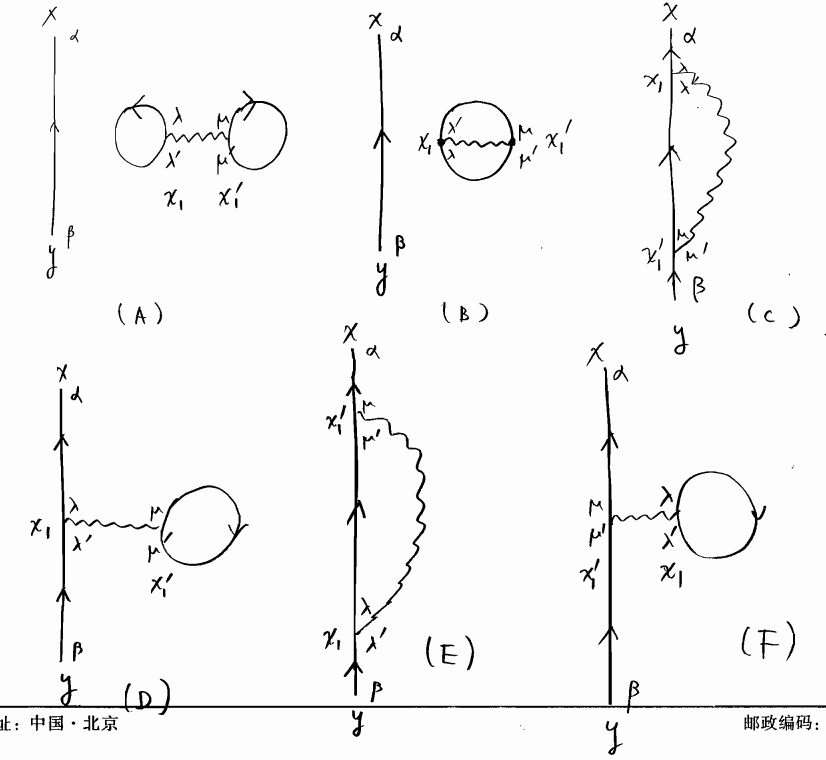
\includegraphics[width = 12cm]{P245.png}
\end{center}
In this pictorial description, single-particle non-interacting green function $G^0$ is denoted by a straight line, with an arrow which runs from the second argument of $G^0$ to the first argument of $G^0$.

The interaction potential is denoted by a wavy line, so that ???

	There are several features in these first order expressions.

1.First of all, these three terms contain a green's function whose two arguments are at the same time.
\begin{align}
\mathrm{i}G^0_{\alpha\beta}(x,x)\stackrel{?}{=}\langle\Phi_0|\mathrm{T}[\hat \psi_{\alpha}({\bf x},t)\hat \psi_{\beta}^{\dagger}({\bf x},t)]|\Phi_0\rangle \nonumber
\end{align}
By definition, such a green function (has an ambiguity, in a sense that it) could be either this or this.
\begin{align}
\stackrel{?}{=}
\begin{cases}
\langle\Phi_0|\hat \psi_{\alpha}({\bf x},t)\hat \psi_{\beta}^{\dagger}({\bf x},t)|\Phi_0\rangle  \cr \langle\Phi_0|\hat \psi_{\alpha}({\bf x},t)\hat \psi_{\beta}^{\dagger}({\bf x},t)|\Phi_0\rangle
\end{cases}
\nonumber
\end{align}
This ambiguity comes from the interaction Hamiltonian, where two creation operators and two annihilation operator have the same time argument
$$(r.h.s)=\langle\Phi_0|\mathrm{T}[\hat \psi_{\lambda}^{\dagger}(x_1)\hat \psi_{\mu}^{\dagger}(x_1')\hat \psi_{\mu'}(x_1')\hat \psi_{\lambda'}(x_1)\hat \psi_{\alpha}(x)\psi^{\dagger}_{\beta}(y)]|\Phi_0\rangle $$
To remove this ambiguity, we take the time argument of the two creation fields to be infinitesimally later than the time argument of the two annihilation fields.
$$(r.h.s)=\langle \Phi_0|\mathrm{T}[\hat \psi_{\lambda}^{\dagger}({\bf x}_1,t_1+0)\hat \psi_{\mu}^{\dagger}({\bf x}_1',t_1+0)\hat \psi_{\mu'}^{\dagger}({\bf x}_1',t_1)\hat \psi_{\lambda'}^{\dagger}({\bf x}_1,t_1)\hat \psi_{\alpha}(x)\hat \psi^{\dagger}_{\beta}(y)]|\Phi_0\rangle$$
This treatment is ok, because under the time-ordered product, this infinitesimally small factor can maintain the order of these four fields in the interaction Hamiltonian.

This small factor results in a small factor here so that, the green's function at equal times must be interpreted in this way.
\begin{align}
\mathrm{i}G_{\alpha\beta}^{0}(x,x)\equiv& \lim_{t'\rightarrow t+0} \langle \Phi_0 | \mathrm{T}[\hat\psi_{\alpha}({\bf x},t)\hat{\psi_{\beta}^{\dagger}}({\bf x},t')]|\Phi_0\rangle \nonumber \\
=&-\langle \Phi_0 |\hat{\psi_{\beta}^{\dagger}}({\bf x},t)\hat\psi_{\alpha}({\bf x},t)|\Phi_0\rangle \nonumber \\
=&-\delta_{\alpha\beta}n^0({\bf x}) \nonumber
\end{align}
where $n^0(x) $ is the particle density at x in the non-interacting ground state wave function.

For a uniform system, this can be replaced by a constant(N/V).

2. 2nd important features in this expression is that these two terms are  disconnected diagrams, in a sense that they contain subunits that are not connected to the rest of the diagrams.

eq.\ref{2.5.2}shows that such disconnected diagrams typically have green's function and interaction whose arguments close within themselves.

As a result, these disconnected subunits can be factorized in the expression for $\tilde{G}$.

To see this, let us substitute eq.\ref{2.5.2} into eq.\ref{2.5.1} .
\begin{align}
\mathrm{i}\tilde{G_{\alpha\beta}}(x,y)=&\mathrm{i}\hat{G_{\alpha\beta}^0}(x,y)+(\frac{-\mathrm{i}}{\hbar})\sum_{\lambda\lambda'\mu\mu'}\frac{1}{2}\int\mathrm{d}^4x_1\mathrm{d}^4x_1' \nonumber \\
&\times \hat{U}_{\lambda\lambda'\mu\mu'}(x_1,x_1') \nonumber \\
&\times\{\mathrm{i}G_{\alpha\beta}^0(x,y)[\mathrm{i}G^0_{\mu'\mu}(x_1',x_1')\mathrm{i}G^0_{\lambda'\lambda}(x_1,x_1)-\mathrm{i}G^0_{\mu'\lambda}(x_1',x_1)\mathrm{i}G^0_{\lambda'\mu}(x_1,x_1')]\nonumber \\
&\ \ +(C)+(D)+(F)+(E)\} \nonumber
\end{align}
Since the arguments of this non-interacting green's function has nothing to do with these integral variables, we can rewrite this as
\begin{align}
=&\{\mathrm{i}G_{\alpha\beta}^0(x,y)+(\frac{-\mathrm{i}}{\hbar})\sum_{\lambda\lambda'\mu\mu'}\frac{1}{2}\int\mathrm{d}^4x_1\mathrm{d}^4x_1' \nonumber \\
&\ \ \hat{U}_{\lambda\lambda'\mu\mu'}(x_1,x_1')[(C)+(D)+(E)+(F)]+...\} \nonumber \\
&\times \{1+(\frac{-\mathrm{i}}{\hbar})\sum_{\lambda\lambda'\mu\mu'}\frac{1}{2}\int\mathrm{d}^4x_1\mathrm{d}^4x_1'\hat{U}_{\lambda\lambda'\mu\mu'}(x_1,x_1') \nonumber \\
&\ \ [\mathrm{i}G^0_{\mu'\mu}(x_1',x_1')\mathrm{i}G^0_{\lambda'\lambda}(x_1,x_1)-\mathrm{i}G^0_{\mu'\lambda}(x_1',x_1)\mathrm{i}G^0_{\lambda'\mu}(x_1,x_1')]+...\} \nonumber
\end{align}
where the product between this \& this gives the 0th order, while the product between this and these two give the 1st order disconnected diagrams, namely (A)\&(B) respectively.

On the other hand, the product between this 4 terms and this gives the 1st order connected diagrams, namely (C),(D),(E),(F).

One might also wonder about the product between these four \& these two.

Such a product reproduce exactly some of the 2nd-order disconnected diagrams obtained from the 2nd-order expansions.

To perform this factorization more systematically, let us consider the $\nu$-th order term of the numerator of eq.\ref{2.4.4}:

\begin{align}
\mathrm{i}G_{\alpha\beta}^{(\nu)}(x,y)\equiv(\frac{-\mathrm{i}}{\hbar})^{\nu}\frac{1}{\nu!}\int_{-\infty}^{\infty}\mathrm{d}t_1...\int_{-\infty}^{\infty}\mathrm{d}t_{\nu}\langle\Phi_0|\mathrm{T}[\hat H_1(t_1)\hat H_1(t_2)...\hat H_1(t_{\nu})\hat \psi_{\alpha}(x)\hat \psi^{\dagger}_{\beta}(y)]|\Phi_0\rangle \nonumber
\end{align}
In general, $\nu$-numbers of interaction Hamiltonians can be divided into n-numbers of those interaction Hamiltonians which are connected to\ \ the fermion line running from y to x\ \ and m-numbers of those interaction Hamiltonians which are disconnected from the fermion line.
\begin{center}
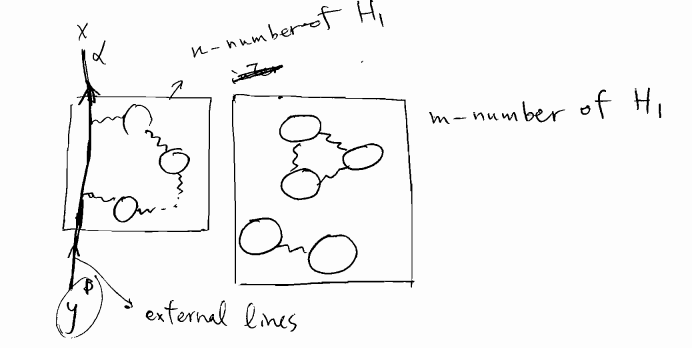
\includegraphics[width = 10cm]{P255.png}
\end{center}
The arguments appearing in the former group and those in the latter are nothing to do with each other, so that we can rewrite this into a product between two totally disconnected factors.

\begin{align}
\mathrm{i}\tilde{G}_{\alpha\beta}^{(\nu)}(x,y)=& \sum_{n=0}^{\nu}\sum_{m=0}^{\nu}(\frac{-\mathrm{i}}{\hbar})^{n+m}\frac{1}{\nu!}\frac{\nu!}{n!m!} \nonumber \\
&\int_{-\infty}^{\infty}\mathrm{d}t_1...\int_{-\infty}^{\infty}\mathrm{d}t_{m}\langle\Phi_0|\mathrm{T}[\hat H_1(t_1)...\hat H_1(t_{m})\hat \psi_{\alpha}(x)\hat \psi^{\dagger}_{\beta}(y)]|\Phi_0\rangle_{connected} \nonumber \\
&\int_{-\infty}^{\infty}\mathrm{d}t_{m+1}...\int_{-\infty}^{\infty}\mathrm{d}t_{m+n}\langle\Phi_0|\mathrm{T}[\hat H_1(t_{m+1})...\hat H_1(t_{m+n})\hat \psi_{\alpha}(x)\hat \psi^{\dagger}_{\beta}(y)]|\Phi_0\rangle \nonumber 
\end{align}
Here we put subscript 'connected', in order to emphasize that the contractions here must be taken in the 'connected' way like this diagram.

We also put this factor, because the numbers of ways of dividing $\nu$-number of interaction Hamiltonians in to n- number of the former group and m-number of the latter group is given by the factorial of $\nu$ divided by that of m times that of n.

When summed over the integer $\nu$ from zero to infinite, we obtain the numerator of eq.\ref{2.4.4} as follows
\begin{align}
\mathrm{i}\tilde{G}_{\alpha\beta}^{(\nu)}(x,y)=& \sum_{m=0}^{\infty}(\frac{-\mathrm{i}}{\hbar})^{m}\frac{1}{m!}\int_{-\infty}^{\infty}\mathrm{d}t_1...\int_{-\infty}^{\infty}\mathrm{d}t_{m}\langle\Phi_0|\mathrm{T}[\hat H_1(t_1)...\hat H_1(t_{m})\hat \psi_{\alpha}(x)\hat \psi^{\dagger}_{\beta}(y)]|\Phi_0\rangle_{connected} \nonumber \\
&\times\sum_{m=0}^{\infty}(\frac{-\mathrm{i}}{\hbar})^{n}\frac{1}{n!}\int_{-\infty}^{\infty}\mathrm{d}t_1...\int_{-\infty}^{\infty}\mathrm{d}t_{n}\langle\Phi_0|\mathrm{T}[\hat H_1(t_1)...\hat H_1(t_{n})\hat \psi_{\alpha}(x)\hat \psi^{\dagger}_{\beta}(y)]|\Phi_0\rangle\nonumber 
\end{align}
Here the first factor is the sum of all connected Feynman diagrams.

On the other hand, the 2nd factor is identical to the denominator of eq.\ref{2.4.4}
\begin{align}
\langle\Phi_0|\hat{S}|\Phi_0\rangle=&\langle\Phi_0|\hat{U}(+\infty,-\infty)|\Phi_0\rangle \nonumber \\
=&\langle\Phi_0|\sum_{\nu=0}^{\infty}(\frac{-\mathrm{i}}{\hbar})^{\nu}\frac{1}{\nu!}\int_{-\infty}^{\infty}\mathrm{d}t_1...\int_{-\infty}^{\infty}\mathrm{d}t_{\nu}\mathrm{T}[\hat H_1(t_1)...\hat H_1(t_{\nu})]|\Phi_0\rangle\nonumber 
\end{align}
So that the second factor are set off by the denominator, and eq.\ref{2.4.4} is given by the sum of all possible connected Feynman diagrams.
\begin{align} \label{2.5.3}
\mathrm{i}G_{\alpha\beta}(x,y)=& \sum_{m=0}^{\infty}(\frac{-\mathrm{i}}{\hbar})^{m}\frac{1}{m!}\int_{-\infty}^{\infty}\mathrm{d}t_1...\int_{-\infty}^{\infty}\mathrm{d}t_{m}\langle\Phi_0|\mathrm{T}[\hat H_1(t_1)...\hat H_1(t_{m})\hat \psi_{\alpha}(x)\hat \psi^{\dagger}_{\beta}(y)]|\Phi_0\rangle
\end{align}
This formula for single-particle green's function is very useful, because it allows us to ignore all disconnected Feynman diagrams, which contain subunits not connected to the fermion line running from y to x.

3. The 3rd important remark is that, for any given connected diagram, there are many similar diagrams that differ in the permutation of the labels in the interaction Hamiltonian $\hat H_1$.

For example, these two diagrams 
\begin{center}
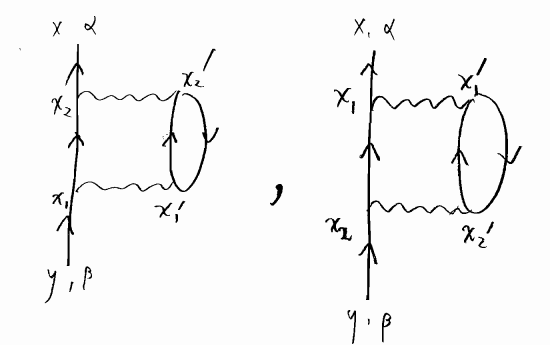
\includegraphics[width = 8cm]{P260.png}
\end{center}
differ from each other only in the permutation of the labels 1 \& 2 associated with the interaction Hamiltonian.

When these arguments are integrated oyut, these two give an identical contribution.

Another example is the 3rd order connected diagram shown here.
\begin{center}
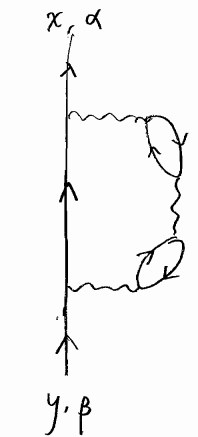
\includegraphics[width = 2cm]{P261.png}
\end{center}
Depending on how we assign three interaction Hamiltonians to these there wavy lines, we have 6 similar connected diagrams.

All of these six gives an identical contribution to the green's function.

For a m-th ordered connected diagram, we generally have the factorial of m number of similar diagrams, which differ in the permutations and all of which give an identical contribution.

This, 'the factorial of m' cancel the factor here.

Thus, for a given topologically distinct connected Feynman diagram, we count only once, while omitting this prefactor.

Here the 'topological distinct' means as follows

We regard that two diagrams are topologically distinct, when they cannot be transformed to each other, by any kind of deformation of wavy lines (interaction Hamiltonians).
\begin{center}
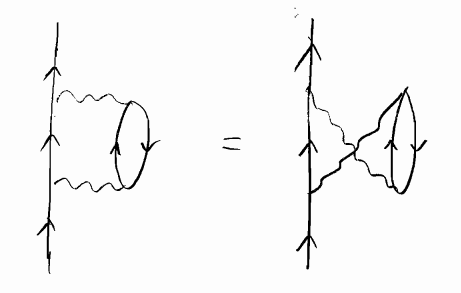
\includegraphics[width = 6cm]{P263.png}
\end{center}
4. Note also that, in the first order examples shown in eq.\ref{2.5.2}, the terms (C)\&(E) are equal to each other.

They differ only in that x\&x' are interchanged, while the potential is symmetric under this interchange
$$U_{\lambda\lambda',\mu\mu'}(x,x')=U_{\mu\mu',\lambda\lambda'}(x',x)$$
Accordingly, it is sufficient to retain just one of these two, while omitting prefactor $\frac{1}{2}$ which appears in $\hat V$ in eq.\ref{2.3.3}


The same is true for (D)\&(F).

We therefore obtain the following rules for calculating the n-th order contribution to the single particle green's function.

(a) Draw all topologically distinct connected Feynman diagrams, with n-interaction lines U and (2n+1) directed green's function $G^0$

(b) Label each vertex with a for dimensional space-time coordinate.

(c) Each solid line represents a green's function $G_{\alpha\beta}^0(x,y)$ running for y to x.

(d) Each wavy lines represents an interaction.
\begin{center}
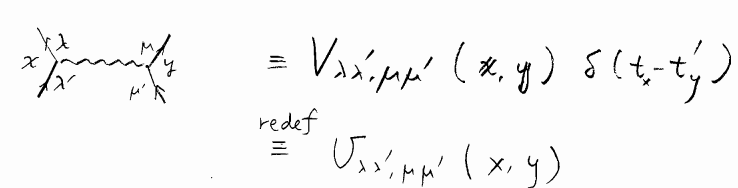
\includegraphics[width = 10cm]{P266.png}
\end{center}
(e) integrate all the internal variables over space and time.

(f) take the sum over all the spin indices associated with internal lines.

Since the n-th order term in eq.\ref{2.5.3} has an explicit numerical factor $(\frac{-\mathrm{i}}{\hbar})^n$

Each contraction of two field operators gives $\mathrm{i}G^0$, so that (2n+1) contractions of the field operators gives $(\mathrm{i})^{2n+1}$

(g) for each n-th order term for G, assign $(-\mathrm{i})(\mathrm{i})^{2n+1}(\frac{-\mathrm{i}}{\hbar})^n=(\frac{-\mathrm{i}}{\hbar})^n$

in addition to this, each Feynman diagram must be accompanied by  either (+) or (-) sign, which comes from the rearrange process of the field operators.

Namely, when we obtained eq.\ref{2.5.2}, we have rearranged the order of operators, in such a way that two field operators that are contracted are brought together.

Depending on whether this rearrange process is accompanied by even numbers of permutations of field operators or odd numbers of the permutations, each Feynman diagram is accompanied by (+) or (-) sign respectively.

Generally, a Feynman diagram with F-numbers of loops composed by fermion lines is accompanied by $(-1)^F$
\begin{center}
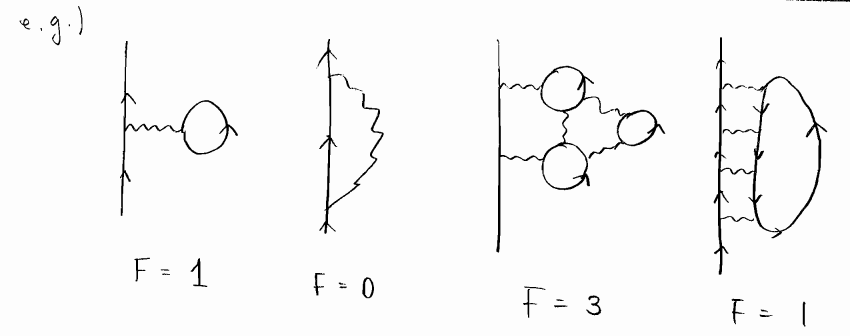
\includegraphics[width = 12cm]{P270-1.png}
\end{center}
This can be in the following way.

Generally speaking, any loop in a Feynman diagram is given like this.
\begin{center}
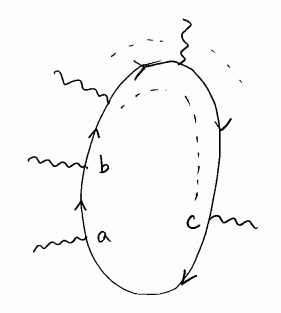
\includegraphics[width = 3cm]{P270-2.png}
\end{center}

On the one hand, according to eq.(A), the starting order of the field operators is given like this.

$$\mathrm{T}[\hat H_1(t_1)...\hat H_1(t_a)...\hat H_1(t_b)...\hat H_1(t_c)...\hat H_1(t_m)\hat \psi_{\alpha}(x)\hat \psi_{\beta}^{\dagger}(y)]$$
\begin{center}
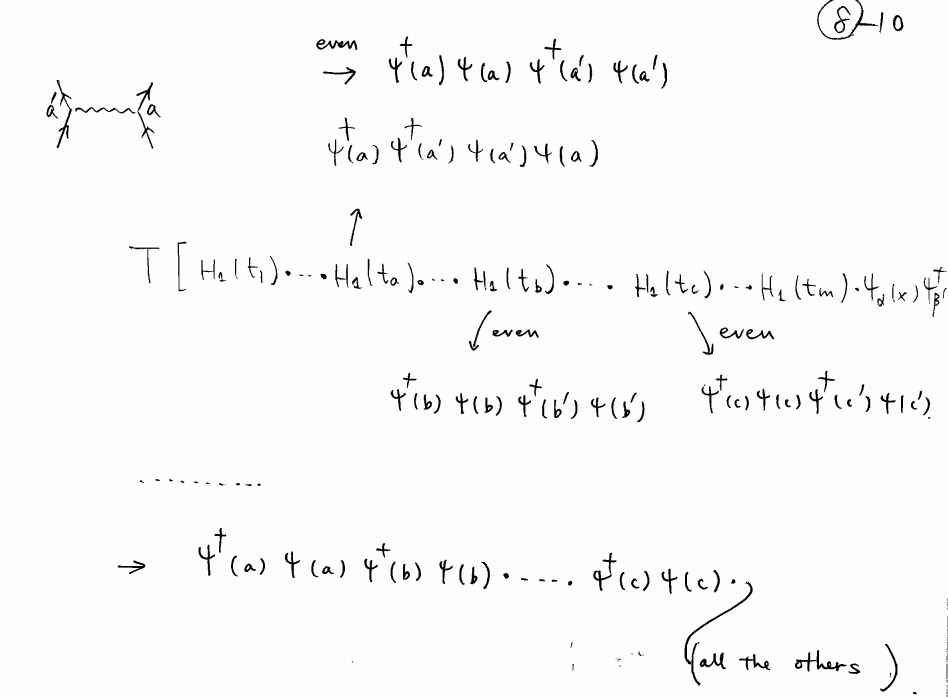
\includegraphics[width = 14cm]{P271.png}
\end{center}
Where these three interaction Hamiltonians correspond to these three wavy lines respectively.

Each interaction Hamiltonian can be given like this, and corresponding Feynman diagram is depicted like this.

Under the time-ordered product, we can rearrange this like this with even number of permutation.

Similarly we can do this for other interaction Hamiltonians.
\begin{center}
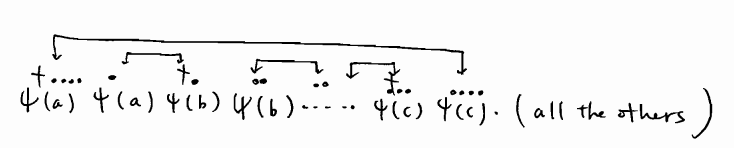
\includegraphics[width = 12cm]{P273.png}
\end{center}

Now that this part corresponds to this part and this part corresponds to this part, so that we bring them together like this.

This rearranging process is accompanied by even number of permutations, because these pairs of two fields always move together.

Then, according to this diagram, we take contractions like this.
\begin{center}
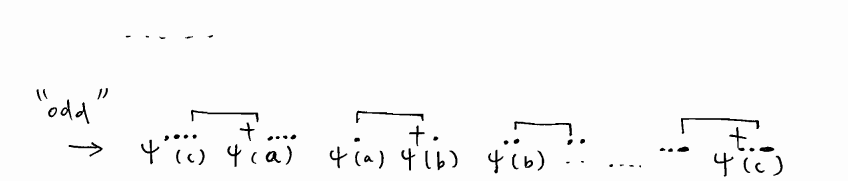
\includegraphics[width = 11cm]{P275.png}
\end{center}

Then, most of the two fields that are contracted are already brought together, except for these two fields.

But, when we bring together these two, we always need odd numbers of permutations.

This concludes that, for each loop of fermion fields, we always have one minus sign.
\begin{center}
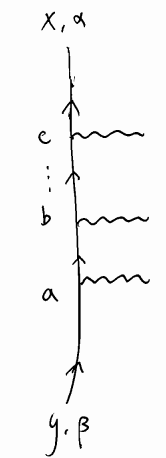
\includegraphics[width = 2cm]{P277.png}
\end{center}

We can do the same procedure for the other loops which you can find within all the others.

By construction, the remaining fermion fields comprise a single fermion lines which runs from y to x, where and x are associated with the external fermion fields which can be depicted like this
\begin{align}
&\mathrm{T}[\hat H_1(t_1)...\hat H_1(t_a)...\hat H_1(t_b)...\hat H_1(t_c)...\hat H_1(t_m)\hat \psi_{\alpha}(x)\hat \psi_{\beta}^{\dagger}(y)]\nonumber \\
=&(-1)^F\mathrm{T}[(loop1)(loop2)...(loopF)\hat \psi^{\dagger\cdot\cdot\cdot\cdot\cdot}(a)\hat \psi^{\cdot}(a)\hat \psi^{\cdot\cdot\cdot\cdot}(b)...\hat \psi^{\dagger\cdot\cdot\cdot}(c)\hat \psi^{\cdot\cdot\cdot\cdot}(c)\hat \psi_{\alpha}^{\cdot\cdot\cdot\cdot}(x)\hat \psi_{\beta}^{\dagger\cdot\cdot\cdot\cdot}(y)]\nonumber
\end{align}
With even number of permutations, all the remaining fermion fields can be rearranged in this way.

According to this picture, we take the contraction like this, where most of the two fields that are contracted are already brought together.

except for these two field.

When we bring together these two, we need even number of permutations, because here we have even numbers of field operators.
\begin{align}
=&(-1)^F\mathrm{T}[(loop1)(loop2)...(loopF)(the\ single\ fermion\ line)]\nonumber
\end{align}
This gives us this expression for this.

(h) To summarize, a Feynman diagram with F-numbers of fermion loops is always accompanied by $(-1)^F$

This is the 2nd last rule for the Feynman diagram calculations.

The final rule is for a non-interacting single particle green's function with equal time variables.

As I have already explained, the green's function with equal time variables should be interpreted as this way

(i) $G_{\alpha\beta}^0(x,t;x',t')\rightarrow G_{\alpha\beta}^0(x,t;x',t+0)$

\begin{center}
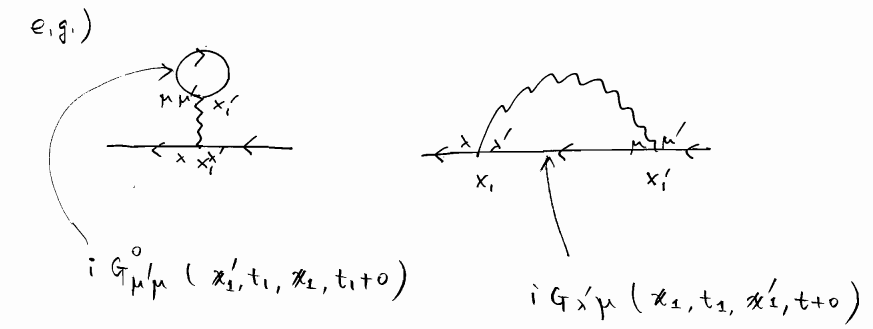
\includegraphics[width = 13cm]{P283.png}
\end{center}


This is all about the rules for the Feynman diagram calculations.

Based on this Feynman's rules, let us again calculate the 1st-order contribution to the single-particle green's function.

$$G_{\alpha\beta}^{(1)}(x,y)=?$$
Only the topologically distinct connected Feynman diagrams are just these two.
\begin{center}
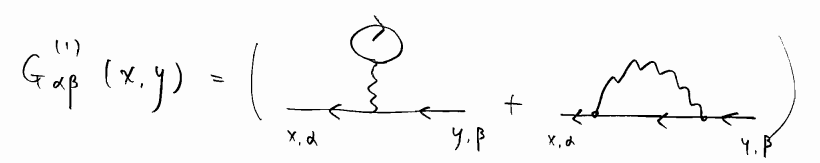
\includegraphics[width = 12cm]{P284-1.png}
\end{center}
By labelling these vertex four dimensional coordinate,
\begin{center}
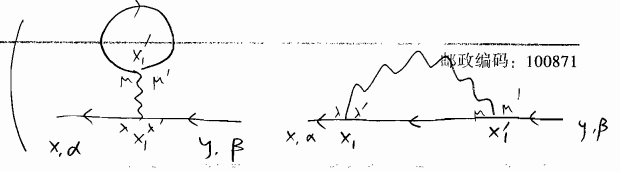
\includegraphics[width = 8cm]{P284-2.png}
\end{center}

According to the rule, we assign each fermion line with $G^0$ and a wavy line with V. so that we obtain

\begin{align}\label{2.5.4}
G_{\alpha\beta}^{(1)}(x,y)=&(\frac{\mathrm{i}}{\hbar})\int \mathrm{d}^4x_1\int \mathrm{d}^4x_1' \nonumber \\
&\{-U_{\lambda\lambda'\mu\mu'}(x_1,x_1')G_{\alpha\lambda}^0(x,x_1)G_{\lambda'\beta}^0(x_1,y)G_{\mu'\mu}^0(x_1',x_1') \nonumber \\
&\ +U_{\lambda\lambda'\mu\mu'}(x_1,x_1')G_{\alpha\lambda}^0(x,x_1)G_{\lambda'\mu}^0(x_1,x_1')G_{\mu'\beta}^0(x_1',y)\} 
\end{align}

The second-order contribution can be enumerated like this.
\begin{center}
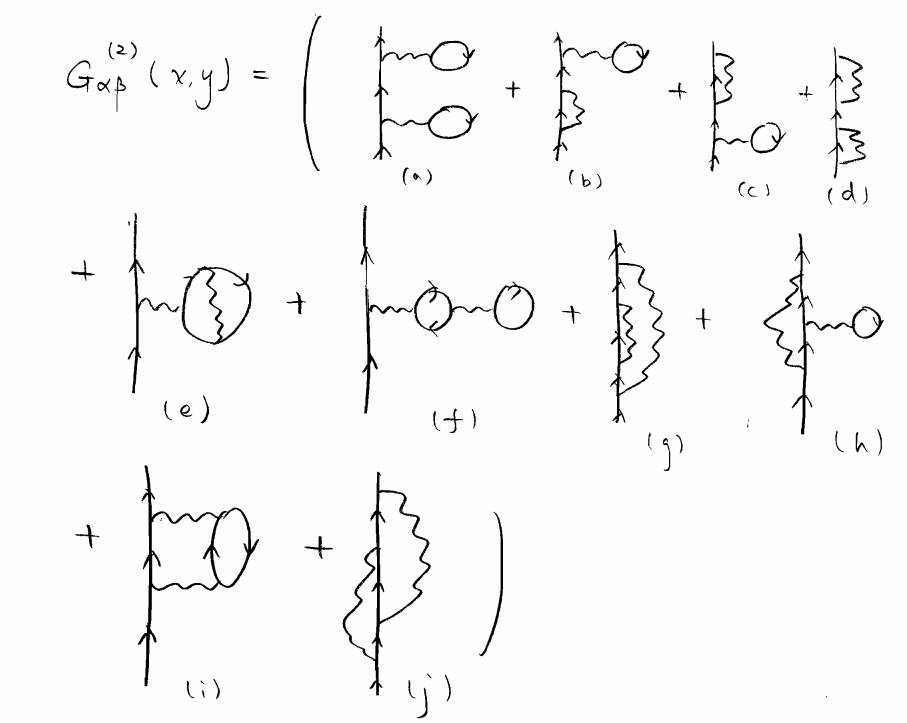
\includegraphics[width = 13cm]{P286.png}
\end{center}
which exhaust all the 2nd-order topologically distinct connected diagrams.

Writing the corresponding equations for all of these diagrams is a bit cumbersome, so that I only write down one of them.

For example, consider the lase one
\begin{center}
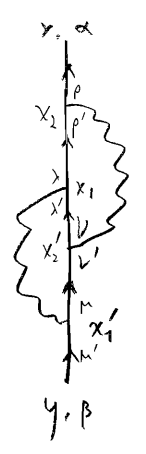
\includegraphics[width = 2cm]{P287.png}
\end{center}
\begin{align}
G^{(2)}_{\alpha\beta}(x,y)=...&+(\frac{\mathrm{i}}{\hbar})^2\int \mathrm{d}^4x_1\int \mathrm{d}^4x_1'\int \mathrm{d}^4x_2\int \mathrm{d}^4x_2'U_{pp'\nu\nu'}(x_2,x_2')U_{\lambda\lambda'\mu\mu'}(x_1,x_1') \nonumber \\
&G_{\alpha\beta}^0(x,x_2)G_{p\lambda}^0(x_2,x_1)G_{\lambda'\nu}^0(x_1,x_2')G_{\nu'\mu}^0(x_2',x_1')G_{\mu'\beta}^0(x_1',y) \nonumber
\end{align}
Here, we don't have any (-) sign, because the diagram doesn't contain any fermion's loop.

Observing this expression, one can see that actual evaluations of each terms are highly involved, in a sense that, even 2nd order term requires integral over four internal variables.

To reduce these complications, let us now restrict the following discussions to a spatially uniform (and spin-isotropic) system.

In such a system, the green's function take the form like this 
$$G_{\alpha\beta}(x,y)=G_{\alpha\beta}(x-y)$$

This form allows us to take a fourier transformation
\begin{align}\label{2.5.5}
G_{\alpha\beta}(x,y)\equiv\frac{1}{(2\pi)^4}\int \mathrm{d}^4ke^{\mathrm{i}k(x-y)}G_{\alpha\beta}(k) \nonumber \\
G^0_{\alpha\beta}(x,y)\equiv\frac{1}{(2\pi)^4}\int \mathrm{d}^4ke^{\mathrm{i}k(x-y)}G^0_{\alpha\beta}(k)
\end{align}
with
$$\mathrm{d}^4k=\mathrm{d}^3\bf{k}\mathrm{f}\omega$$

$$k\cdot x=\bf{k}\cdot\bf{x}-\omega t$$
In a spatially homogeneous system, the interaction potential depends only on the coordinate difference.
\begin{align}\label{2.5.6}
U(x,x')\equiv& V(\bf{x},\bf{x}')\delta(t-t') \nonumber \\
=& V(\bf{x}-\bf{x}')\delta(t-t')
\end{align}
Such a potential can be also fourier-transformed
$$U_{\alpha\alpha\beta\beta'}(x,x')\equiv \frac{1}{(2\pi)^4}\int \mathrm{d}^4ke^{\mathrm{i}k(x-x')}U_{\alpha\alpha\beta\beta'}(k)$$
where
\begin{align}\label{2.5.7}
U_{\alpha\alpha\beta\beta'}(k)=\int \mathrm{d}^3x e^{-\mathrm{i}\bf{k}\cdot\bf{x}}V_{\alpha\alpha\beta\beta'}({\bf x}) \ \ (E)
\end{align}
(with the use of $\delta(t)=\frac{1}{2\pi}\int \mathrm{d}\omega e^{-\mathrm{i}\omega t}$)

Using this transformation, eq.\ref{2.5.4} can be substantially simplified:
\begin{center}
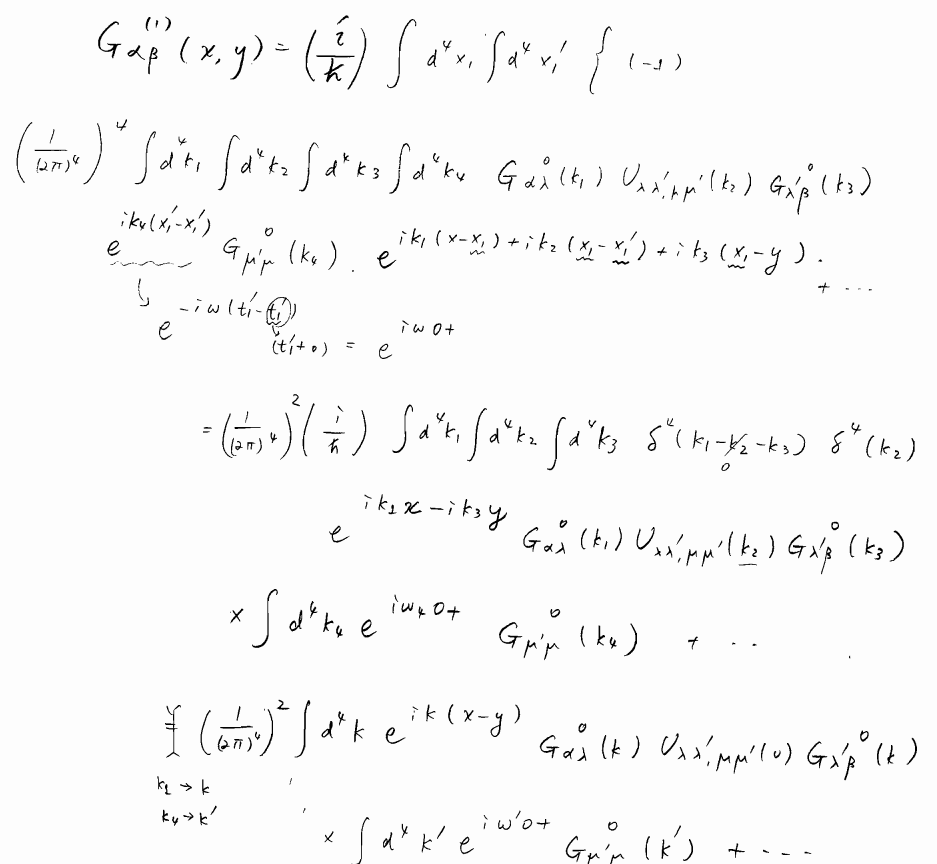
\includegraphics[width = 15cm]{P291.png}
\end{center}\begin{center}
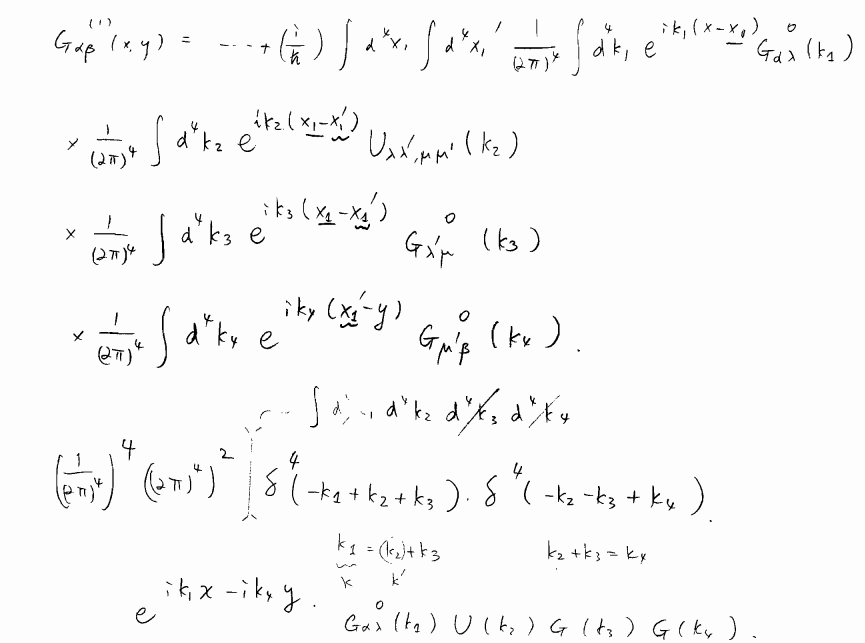
\includegraphics[width = 15cm]{P292.png}
\end{center}
\begin{align}
G_{\alpha\beta}^{(1)}(x,y)=&-\frac{\mathrm{i}}{\hbar}(\frac{1}{(2\pi)^4})^2\int \mathrm{d}^4ke^{\mathrm{i}k(x-y)}G_{\alpha\lambda}^0(k)U_{\lambda\lambda'\mu\mu'}(0)G_{\lambda'\beta}^0(k)\int \mathrm{d}^4k'e^{\mathrm{i}\omega'0+}G_{\mu'\mu}^0(k')\nonumber \\
&+\frac{\mathrm{i}}{\hbar}(\frac{1}{(2\pi)^4})^2\int \mathrm{d}^4ke^{\mathrm{i}k(x-y)}\int \mathrm{d}^4k'G_{\alpha\lambda}^0(k)U_{\lambda\lambda'\mu\mu'}(k')G_{\lambda'\mu}^0(k-k')G_{\mu'\beta}^0(k)\nonumber \\
\equiv & (\frac{1}{(2\pi)^4})^2\int \mathrm{d}^4ke^{\mathrm{i}k(x-y)}G_{\alpha\beta}^{(1)}(k) \nonumber
\end{align}
where $G_{\alpha\beta}^{(1)}(k)$ contains only momentum integral.
\begin{align}\label{2.5.8}
G_{\alpha\beta}^{(1)}(k)\equiv &-\frac{\mathrm{i}}{\hbar}(\frac{1}{(2\pi)^4})^2G_{\alpha\lambda}^0(k)U_{\lambda\lambda'\mu\mu'}(0)G_{\lambda'\beta}^0(k)\int \mathrm{d}^4k'e^{\mathrm{i}\omega'0+}G_{\mu'\mu}^0(k') \nonumber \\
&+\frac{\mathrm{i}}{\hbar}(\frac{1}{(2\pi)^4})^2G_{\alpha\lambda}^0(k)G_{\mu'\beta}^0(k)\int \mathrm{d}^4k'U_{\lambda\lambda'\mu\mu'}(k')G_{\lambda'\mu}^0(k-k')\ \ (F)
\end{align}
This momentum space representation can be generalized into the higher-order Feynman diagram.

Any Feynman diagram comprise a vertex show like this, in which one in-coming fermion line and one out-going fermion line and interaction lines meet with on another
\begin{center}
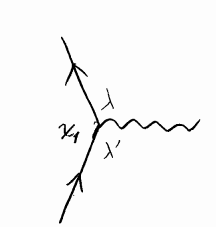
\includegraphics[width = 3cm]{P294.png}
\end{center}
Under the fourier transformation defined in eq.\ref{2.5.5}, the in-coming fermion line provides $e^{\mathrm{i}qx_1}$, and the out-going fermion line provides $e^{-\mathrm{i}q'x_1}$
\begin{center}
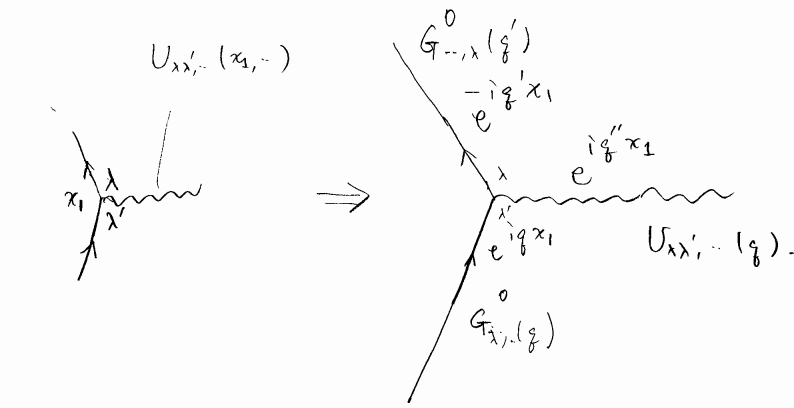
\includegraphics[width = 12cm]{P295.png}
\end{center}

where q and q' are the four-dimensional momenta associated with these two lines.

Namely, we assign this line with $G_{\lambda',...}^0(q)$ and assign this line with $G_{...,\lambda}^0(q')$.

When this interaction potential is given by $U_{\lambda\lambda',...}(x_1,...)$, where we assign the wavy line with $U_{\lambda\lambda',...}(q'')$.


For simplicity, we rewrite this picture like this.
\begin{center}
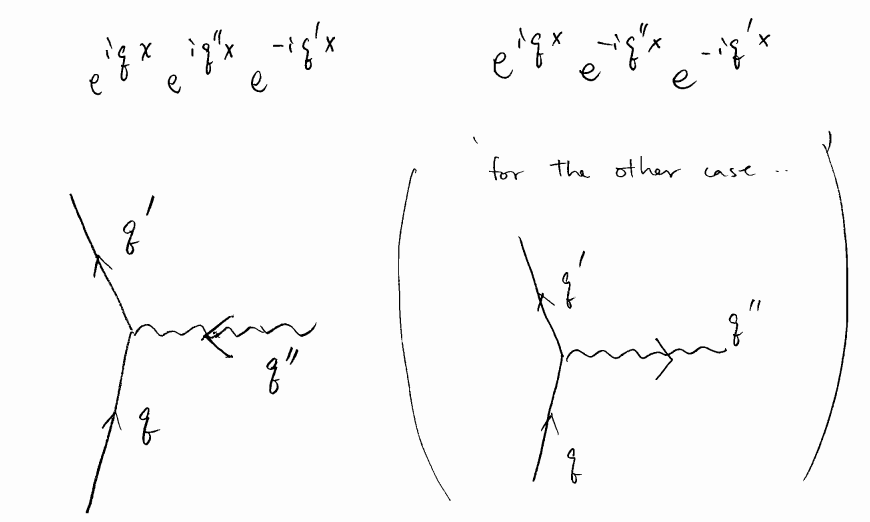
\includegraphics[width = 14cm]{P297.png}
\end{center}
In order to indicate this plus sign, we put another arrow here for the interaction line.

Namely, for this figure, we suppose that these three lines provide $e^{\mathrm{i}qx},e^{\mathrm{i}q''x},e^{-\mathrm{i}q'x}$ respectively.

while for the other case, we suppose that they provide $e^{\mathrm{i}qx},e^{-\mathrm{i}q''x},e^{-\mathrm{i}q'x}$ respectively.

Now that x here is the internal variable, we are supposed to take the integral over this.

Now that, for any given Feynman diagram which have this as its submit, there is no x-dependence other than these three phase factors.

Therefore, the integration over x gives a momentum conservation among these three.

\begin{align}
\int \mathrm{d}^4xe^{\mathrm{i}(q-q'+q'')x}=(2\pi)^4\delta^4(q-q'+q'') \nonumber
\end{align}

Namely, the sum of the two in-coming momenta must be equal to the out-going momentum.


Since every integral vertex provides the momentum conservation law, the in-coming momentum and out-going momentum conservation law, the in-coming momentum and out-going momentum for the external fermion fields are equal to each  other.
\begin{center}
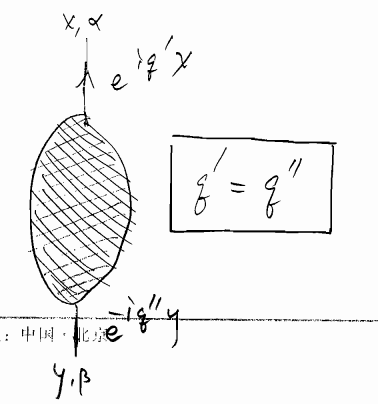
\includegraphics[width = 4cm]{P300.png}
\end{center}
You can check this equality for any Feynman diagram.

As an illustration, consider this 
\begin{center}
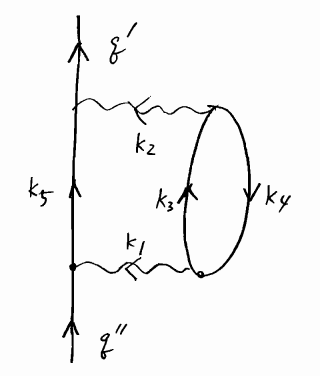
\includegraphics[width = 4cm]{P301.png}
\end{center}
you can assign arrows for wavy lines in an arbitrary way, so that I put this way.

Then we have these conservations for each internal vertex
$$k_5=k_1+q''$$$$k_3+k_1=k_4$$$$k_2+k_4=k_3$$$$q'=k_2+k_5$$$$q'=k_2+k_5=(k_3-k_4)+k_1+q''=k_4-k_4+q''=q''$$

From which  we safely obtain this equality.

To sumarize, the Feynman rule in the momentum space representation can be summarized as follows.

For the n-th order contribution to $$G_{\alpha\beta}({\bf k},\omega)\equiv G_{\alpha\beta}(k)$$

1. Draw all topologically distinct connected diagrams with n-interaction lines and (2n+1) fermion lines.

2. Assign momentum to fermion lines and interaction lines with arrows.

3. Correspondingly, we assign each fermion line with the non-interacting green's fn in the momentum space.(eq.\ref{2.3.6})
$$G_{\alpha\beta}^0({\bf k},\omega)=\delta_{\alpha\beta}[\frac{\theta(|k|-k_F)}{\omega-\omega_k+\mathrm{i}\eta}+\frac{\theta(k_F-|k|)}{\omega-\omega_k-\mathrm{i}\eta}]$$

while we assign each wavy line with the interaction potential in the momentum space representation.
$$U_{\lambda\lambda',\mu\mu'}(q)\equiv V_{\lambda\lambda',\mu\mu'}({\bf q})$$

4. Impose momentum conservations at every internal vertex.

$(2n+1)+n-2n=n+1$

This conservation gives (n+1) independent momentum, where one of them should be reserved for the external line.

Thus we have n independent internal momenta, over which we need to take the integration.

5. Take a summation over internal spin indices.

As an overall factor, we originally have $(\frac{\mathrm{i}}{\hbar})^n(-1)^F$ in the Feynman rule in the real space representation.

During this fourier transformation process, we obtain
$$(\frac{1}{(2\pi)^4})^{2n+1}(\frac{1}{(2\pi)^4})^n((2\pi)^4)^{2n}=(\frac{1}{(2\pi)^4})^{n+1}$$

One of them should be again reserved for the external line, so that

6. For the n-th order Feynman diagram for $G_{\alpha\beta}(k)$, we need to apply $(\frac{\mathrm{i}}{\hbar})^n\frac{1}{(2\pi)^{4n}}(-1)^F$ as an overall factor

The final remark  is about a fermion line that form a closed loop like this or about a fermion line whose two end points are linked by the same interaction link (like this)
\begin{center}
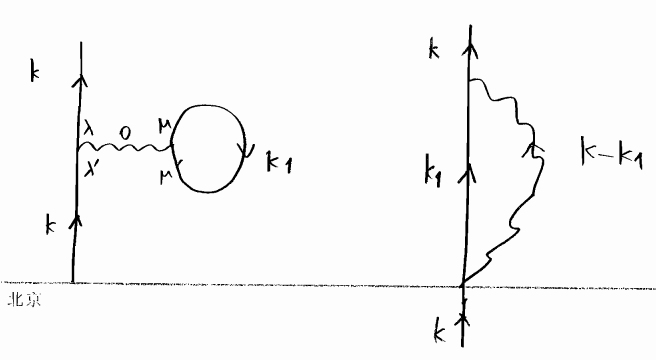
\includegraphics[width = 9cm]{P306.png}
\end{center}
These fermion lines are originally green's function with equal time variables, so that we assigned these green's function to them in this way.

7. When Fourie-transformed, this infinitesimally small factor is transformed with this additional factor, where $\eta$ is positive small quantity:
$$e^{\mathrm{i}\omega\eta}G_{\alpha\beta}({\bf k},\omega) \ \ (\eta\rightarrow0+)$$

With this Feynman rule, one can obtain Eq.\ref{2.5.8}

\begin{align}
G_{\alpha\beta}^{(1)}(k)=&-\frac{\mathrm{i}}{\hbar}\frac{1}{(2\pi)^4} G_{\alpha\lambda}^{(0)}(k)U_{\lambda\lambda'\mu\mu'}(0)G_{\lambda'\beta}^{(0)}(k)\int \mathrm{d}^4k'e^{\mathrm{i}\omega'0+}G_{\mu'\mu}^0(k') \nonumber \\
&+\frac{\mathrm{i}}{\hbar}\frac{1}{(2\pi)^4} G_{\alpha\lambda}^{(0)}(k)G_{\mu'\beta}^{(0)}(k)\int \mathrm{d}^4k'e^{\mathrm{i}\omega'0+}U_{\lambda\lambda'\mu\mu'}(k-k')G_{\lambda'\mu}^0(k') \nonumber
\end{align}

To make further progress, we decompose interaction potential U into spin independent part and spin dependent part 

\begin{align}
U_{\lambda\lambda'\mu\mu'}(q)\equiv& V_{\lambda\lambda'\mu\mu'}(q) \nonumber \\
=& V_0(q) \delta_{\lambda\lambda'}\delta_{\mu\mu'}+V_1(q)\sum_{\nu=1}^{3}[\sigma_{\nu}]_{\lambda\lambda'}[\sigma_{\nu}]_{\mu\mu'} \nonumber
\end{align}

where $\sigma_{1,2,3}$ are Pauli matrices.

Taking $G_{\alpha\beta}^0(k)=\delta_{\alpha\beta}G^0(k)$, we can rewrite eq.\ref{2.5.8} as follows  
\begin{align}
G_{\alpha\beta}^{(1)}(k)=&-\frac{\mathrm{i}}{\hbar}\frac{1}{(2\pi)^4}\delta_{\alpha\lambda}G^{0}(k)
\nonumber \\
&\{V_0(0) \delta_{\lambda\lambda'}\delta_{\mu\mu'}+V_1(0)\sum_{\nu=1}^{3}[\sigma_{\nu}]_{\lambda\lambda'}[\sigma_{\nu}]_{\mu\mu'}\}\delta_{\lambda'\beta}G^0(k)\int \mathrm{d}^4k'e^{\mathrm{i}\omega'0+}\delta_{\mu\mu'}G^0(k')\nonumber \\
&+\frac{\mathrm{i}}{\hbar}\frac{1}{(2\pi)^4}\delta_{\alpha\lambda}G^0(k)\delta_{\mu'\beta}G^0(k)\int \mathrm{d}^4k'e^{\mathrm{i}\omega'0+}\nonumber\\
&\{V_0(k-k') \delta_{\lambda\lambda'}\delta_{\mu\mu'}+V_1(k-k')\sum_{\nu=1}^{3}[\sigma_{\nu}]_{\lambda\lambda'}[\sigma_{\nu}]_{\mu\mu'}\}\delta_{\lambda'\mu}G^0(k') \nonumber \\
with\ \mathrm{Tr}&[\sigma_{\nu}]=0\ \ for \ \nu=1,2,3 \nonumber \\
=&-\frac{\mathrm{i}}{\hbar}\frac{1}{(2\pi)^4}2\delta_{\alpha\beta}G^{0}(k)V_0(0)G^0(k)\int \mathrm{d}^4k'e^{\mathrm{i}\omega'0+}G^0(k')\nonumber \\
&+\frac{\mathrm{i}}{\hbar}\frac{1}{(2\pi)^4}\delta_{\alpha\beta}G^{0}(k)G^0(k)\int \mathrm{d}^4k'V_0(k-k')e^{\mathrm{i}\omega'0+}G^0(k')\nonumber \\
&+\frac{\mathrm{i}}{\hbar}\frac{1}{(2\pi)^4}3\delta_{\alpha\beta}G^{0}(k)G^0(k)\int \mathrm{d}^4k'V_1(k-k')e^{\mathrm{i}\omega'0+}G^0(k')\nonumber \\
\equiv& G^{0}(k)\Sigma^{(1)}(k)G^0(k)\delta_{\alpha\beta} \nonumber \\
\hbar \Sigma^{(1)}(k)=& \mathrm{i}\frac{1}{(2\pi)^4}3\int \mathrm{d}^4k'[-2V_0(0)+V_0(k-k')3V_1(k-k')]e^{\mathrm{i}\omega'0+}G^0(k') \nonumber
\end{align}
Thanks to this factor, we can integrate over frequency

\begin{align}
\int_{-\infty}^{\infty}\frac{\mathrm{d}\omega'}{2\pi}e^{\mathrm{i}\omega'0+}G^0({\bf k}',\omega')=\int_{-\infty}^{\infty}\frac{\mathrm{d}\omega'}{2\pi}e^{\mathrm{i}\omega'0+}[\frac{\theta(|k|-k_F)}{\omega-\omega_k+\mathrm{i}\eta}+\frac{\theta(k_F-|k|)}{\omega-\omega_k-\mathrm{i}\eta}]=\mathrm{i}\theta(k_F-|k'|) \nonumber
\end{align}
\begin{center}
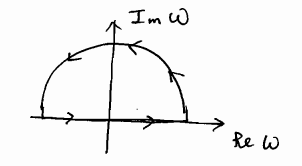
\includegraphics[width = 4cm]{P312.png}
\end{center}
so that
\begin{align}\label{2.5.9}
\hbar \Sigma^{(1)}(k)=&-\int \frac{\mathrm{d}{\bf k}'}{(2\pi)^3}[-2V_0(0)+V_0(k-k')3V_1(k-k')]\theta(k_F-|{\bf k}'|) \nonumber \\
=& n V_0(0)-\int \frac{\mathrm{d}{\bf k}'}{(2\pi)^3}[V_0(k-k')3V_1(k-k')]\theta(k_F-|{\bf k}'|) \ \ (G) 
\end{align}

As we will see soon, these gives us a renormalization of single particle energy in the non-interacting limit.

To see this, let us introduce a general argument which classify various contributions in an arbitrary Feynman diagrams.

The classification leads to a so-called Dyson equation, which makes the diagramatic analysis to be very useful.

Feynman rules suggests that the exact green's function consists of the non-interacting green's function plus all the connected terms with a free ("non-interacting") green's function at each ends.

This structure is schematically shown like this:
\begin{center}
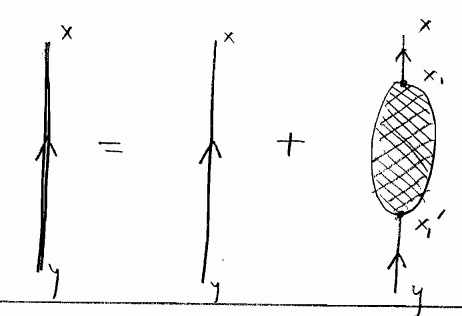
\includegraphics[width = 8cm]{P314.png}
\end{center}
The corresponding analytic expression is given by
$$G_{\alpha\beta}(x,y)=G_{\alpha\beta}^0(x,y)+\int \mathrm{d}^4x_1\int \mathrm{d}^4x_1'G_{\alpha\lambda}^0(x,x_1)\Sigma_{\lambda\mu}(x_1,x_1')G_{\mu\beta}^0(x_1,y)$$

$\Sigma$ corresponds to this part, which includes all the connected Feynman diagrams and is called as the self-energy

2nd-order examples for $\Sigma$ can be enumerated as follows
\begin{center}
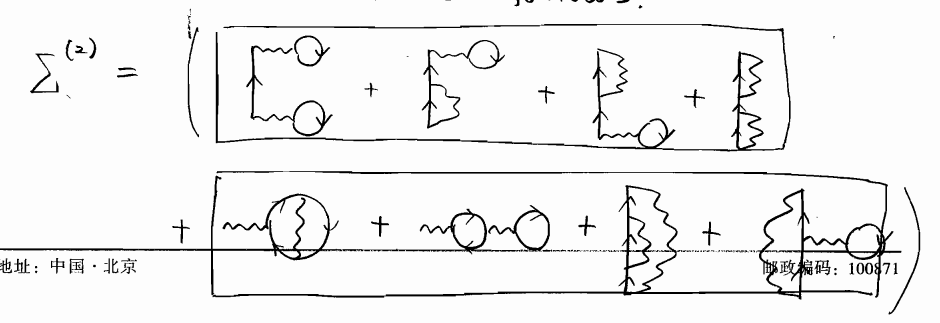
\includegraphics[width = 14cm]{P315.png}
\end{center}
Generally speaking, there are two types of self energy.

One is called as proper self-energy, which cannot be separated into two  pieces by cutting one fermion lines.

The other is called as inproper  self-energy, which can be separated into two pieces by cutting a fermion lines.

In this example, these are inproper ones, because, by cutting this line, they can be separated into two.

Especially, we will denote by $\Sigma^{\star}_{\alpha\beta}(x_1,x_1')$ the sum of all proper self-energy terms.

Then, thanks to the Feynman's rule described so far, the self-energy consists of a sum of all possible repetitions of the proper self-energy.
\begin{align}
\Sigma(x_1,x_1')=&\Sigma^{\star}(x_1,x_1?) \nonumber \\
&+\int \mathrm{d}^4x_2\mathrm{d}^4x_2'\Sigma^{\star}(x_1,x_2)G^0(x_2,x_2')\Sigma^{\star}(x_2',x_1?) \nonumber \\
&+\int \mathrm{d}^4x_2\mathrm{d}^4x_2'\int \mathrm{d}^4x_3\mathrm{d}^4x_3'\Sigma^{\star}(x_1,x_2)G^0(x_2,x_2')\Sigma^{\star}(x_2',x_1?)G^0(x_3,x_3')\Sigma^{\star}(x_3',x_1?)+... \nonumber
\end{align}
Which can be also described in terms of diagram as follows 
\begin{center}
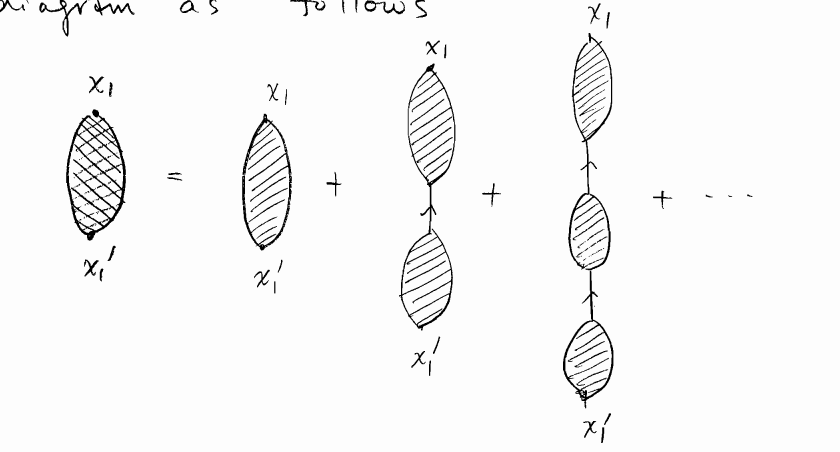
\includegraphics[width = 10cm]{P318.png}
\end{center}
Where this part denotes the proper self-energy, while this fermion line is for non-interacting green's function.

This description becomes possible, especially  because, any n-th order Feynman diagram is accompanied only by $(\frac{\mathrm{i}}{\hbar})^n(-1)^F$ where F denotes the number of fermion loop.

Namely, such a factor can be always decomposed like this
\begin{center}
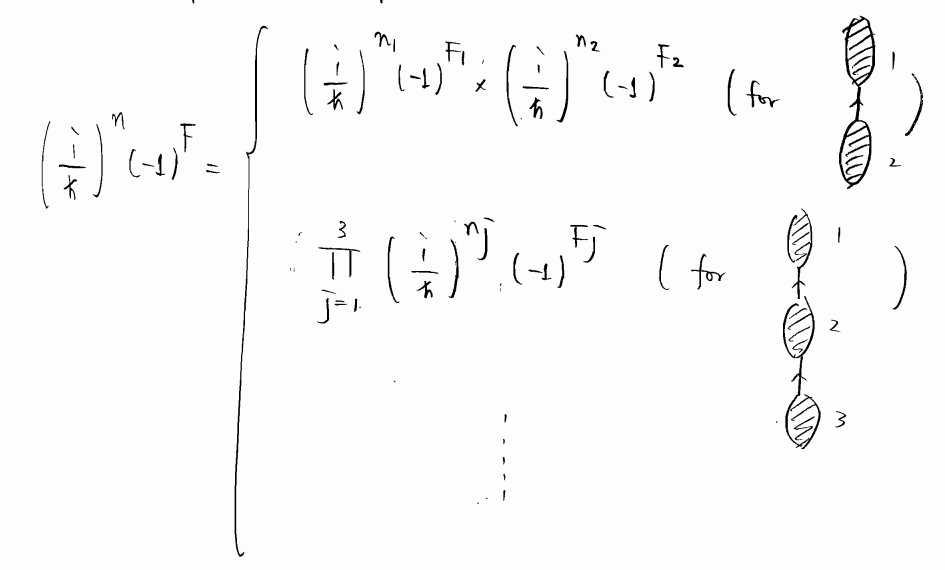
\includegraphics[width = 12cm]{P319.png}
\end{center}
Where $n_1\&n_2$ have denotes the number of wavy lines included in the 1st proper self-energy and 2nd proper self energy. so that $n_1+n_2=n$

Similarly $F_1\&F_2$ denotes the numbers of fermion loops included in these two proper self-energy respectively. so that $F_1+F_2=F$

Correspondingly, the single-particle green's function becomes like this
\begin{align}
G(x,y)=&G^0(x,y) \nonumber \\
&+\int \mathrm{d}^4x_1\mathrm{d}^4x_1'G^0(x,x_1)\Sigma^{\star}(x_1,x_1?)G^0(x_1',y) \nonumber \\
&+\int \mathrm{d}^4x_1\mathrm{d}^4x_1'\int \mathrm{d}^4x_2\mathrm{d}^4x_2'G^0(x,x_1)\Sigma^{\star}(x_1,x_1?)G^0(x_1',x_2)\Sigma^{\star}(x_2,x_2')G^0(x_2',y)+... \nonumber
\end{align}
or
\begin{center}
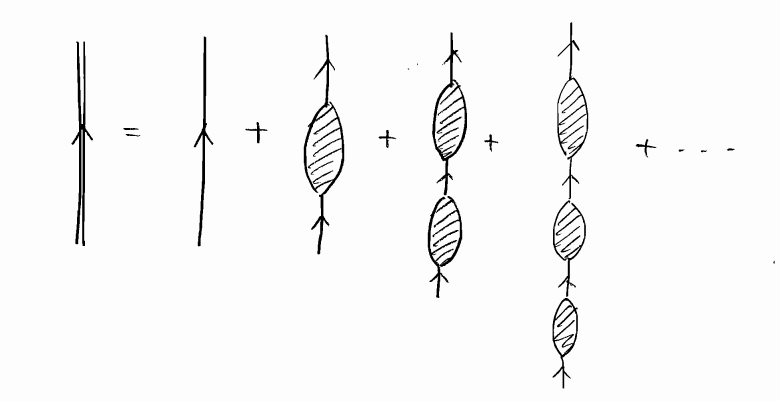
\includegraphics[width = 9cm]{P320.png}
\end{center}
As is clear from this repetitive structure, this can be rewritten also like this.
\begin{center}
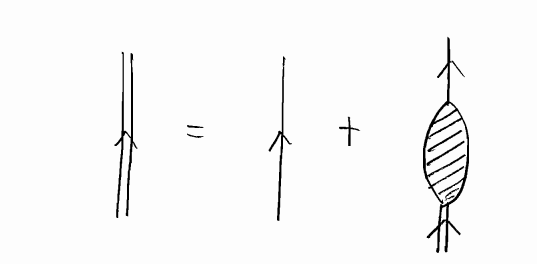
\includegraphics[width = 6cm]{P321.png}
\end{center}
where the lower fermion line is replaced by green's function itself.

Namely, the unknown green's function itself in the left hand side is used for the expression for the green's function, so that the equation becomes a self-consistent equation

This equation is called as Dyson's equation, whose analytic expression is given like this
$$G_{\alpha\beta}(x,y)=G_{\alpha\beta}^0(x,y)+\int \mathrm{d}^4x_1\mathrm{d}^4x_1'G^0_{\alpha\lambda}(x,x_1)\Sigma_{\lambda\mu}^{\star}(x_1,x_1?)G_{\mu\beta}^0(x_1',y)$$
 
By substituting the r.h.s into the left hand side, one can derive this equation out of this.


%323
In the momentum space representation, the Dyson equation become much more simpler. For spatially uniform system, the self-energy can be always Fourier transformed like this

%\begin{align}
\[
\Sigma_{\alpha\beta}^{\star}(x,y) = \frac{1}{(2\pi)^4}\int d^4 k e^{ik(x-y)}\Sigma_{\alpha\beta}^{\star}(k)\]
%\end{align}

With this definition and eq. (2-5-5), the Dyson equation reduces to an algebraic equation: 

\[G_{\alpha\beta}(k) = G^0_{\alpha\beta}(k) + G_{\alpha\lambda}^0(k)\Sigma_{\lambda\mu}^{\star}(k)G_{\mu\beta}(k) \]

For an isotropic system, $G$, $G^0$ and $\Sigma^\star$ becomes diagonal in spin space

\[\begin{split}
G_{\alpha\beta}(k) &= \delta_{\alpha\beta}G(k)\\
G^0_{\alpha\beta}(k) &= \delta_{\alpha\beta}G^0(k)\\
\Sigma^\star_{\alpha\beta}(k) &= \delta_{\alpha\beta}\Sigma^\star_(k)\\
\end{split}\]

As a result, the Dyson equation can be explicitly solved;

\[\begin{split}
&\quad G(k) = G^0(k) + G^0(k)\Sigma^\star(k)G(k)\\
&\Longleftrightarrow (1-G^0(k)\Sigma^\star(k))G(k)=G^0(k)\\
&\Longleftrightarrow G(k) = \frac{1}{{G^0}^{-1}(k)-\Sigma^\star(k)}
\end{split} \]

The inverse of $G^0$ is given by

\[[G^0(k)]^{-1} = \omega - \omega_{\bf k}+i\eta \text{sgn}(|{\bf k}|-k_F) \]

with $\eta\to 0+$

As such, we find

\[G_{\alpha\beta}({\bf k},\omega) = \frac{\delta_{\alpha\beta}}{\omega-\omega_{\bf k}+i\eta\text{sgn}(|{\bf k}|-k_F)}-\Sigma^\star({\bf k},\omega) \]

According to the Lehmann representation, this Green function has a pole above the real axis of $\omega$ when $\omega$ is less than $\mu\hbar$, while it has a pole below the real axis of $\omega$ when $\omega$ is greater than $\mu/\hbar$. 

This general statement ensures the imaginary part of the proper self energy is positive when $\omega$ is less than $\mu/\hbar$, while it is negative otherwise

\[\begin{cases}
\text{Im}\Sigma^\star({\bf k},\omega)\ge 0 &\text{for }\omega\le\mu/\hbar\\
& \\
\text{Re}\Sigma^\star({\bf k},\omega)\le 0 &\text{for }\omega\ge\mu/\hbar
\end{cases}\]

Thanks to this general statement, we can determine the chemical potential in interacting fermion systems as the point at which Im$\Sigma^\star({\bf k},\omega)$ changes the sign. 

In an interacting system, one particle excited state ($a^\dagger_{{\bf k},\lambda}|F.S\rangle (|{\bf k}|>k_F)$) or one-hole excited state ($a_{{\bf k},\lambda}|F.S\rangle (|{\bf k}|<k_F)$) are not an eigenstate of the system, so that these excited particles have a finite life time. Imaginary part of the pole of the Green's function in $\omega<\mu/\hbar$ region describes the life time for the hole, which that in $\omega?\mu/\hbar$ region describes the life time for the particle. 

As an example of the proper self energy, let us consider the first-order \& second-order (Feynman Diagrams)

Within 1st order \& 2nd order, the proper self energies are given like this respectively

\begin{align}
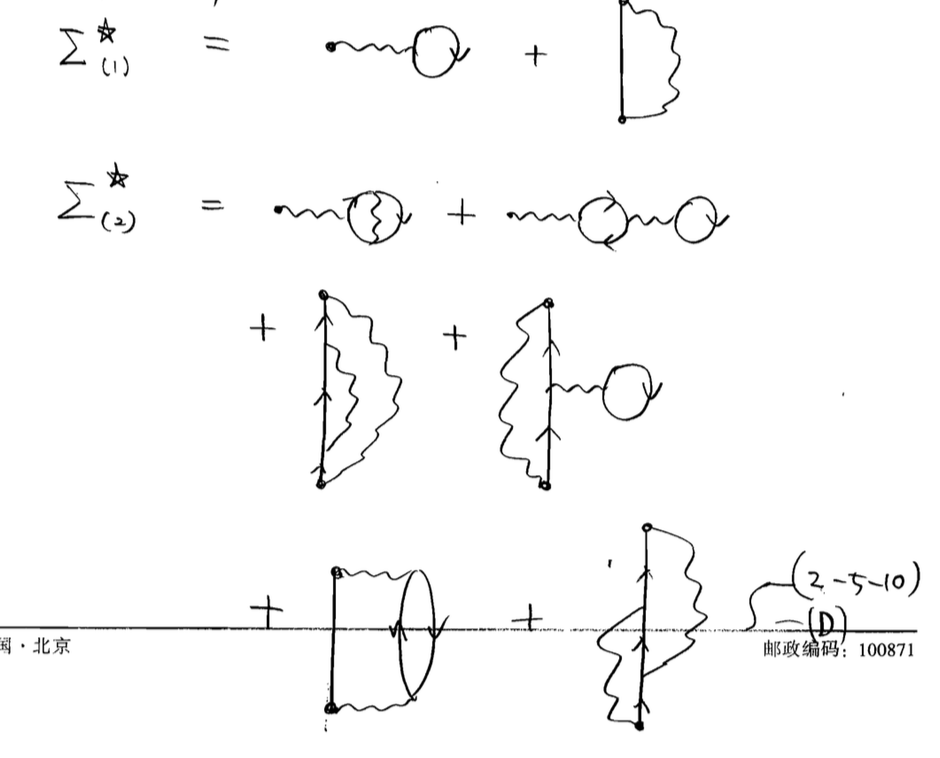
\includegraphics[width = 12cm]{2-5-10D.png}
\end{align}

$\Sigma^\star_{(1)}({\bf k},\omega)$ has been already calculated in eq. (2-5-9):

\[\hbar\Sigma^\star_{(1)} ({\bf k},\omega) = nV_0(0)-\frac{1}{(2\pi)^3}\int d^3{\bf k}'[V_0({\bf k-k}')+3V_1({\bf k-k}')]\theta(k_F-|\bf k|) \]

which does not depend on frequency and which is real valued. 

This means that, within the 1st-order approximation, one-particle state or one-hole state has a infinite life time and effect of the interaction is to change the one-particle spectrum $\omega_{\bf k}$ into another function of $\bf k$

\[\omega_{\bf k}\to\tilde{\omega}_{\bf k} = \omega_{\bf k} + \Sigma^\star_{(1)}({\bf k})=\omega_{\bf k} + \frac{1}{\hbar}nV_0(0) - \frac{1}{\hbar}\int \frac{d{\bf k}'^3}{(2\pi)^3}\times[V_0({\bf k-k}')+3V_1({\bf k-k}')]\theta(k_F-|\bf k'|) \]

Here $nV_0(0)$ is a constant energy shift of the one-particle spectrum, which represents the forward scattering coming from all the other particle. The latter parti represents the exchange scattering. 

Feynman-Dyson perturbation theory developed so far enable us to evaluate the Green's function to all order in the interaction potential. In reality, however, obtaining all order exactly is impossible and we must resort to a certain approximation. As the simplest example, we retained only the first order contribution to the proper self energy. Unfortunately, such an approximation cannot capture the physics of most systems quite well, where inclusions of certain class of higher order terms are necessary. In the following three sections, I will introduce three approximation scheme which goes beyond the 1st-order approximation for the proper self-energy. 


\section{(Self-Consist) Hatree-Fock Approximation}%wsz 2-6

The first approximation scheme is the self-consistant Hartree-Fock approximation, which begins with the 1st order approximation for the proper selfenergy.
\begin{center}
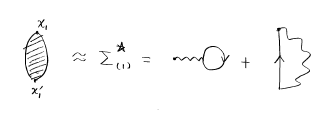
\includegraphics[width = 10cm]{2-6-1.png}\label{Fig2.6.1}
\end{center}


In this approximation, a particle moves in a single particle potential that is created by all the other particles by way of interaction potential. But, in this approximation, these internal fermion lines are just non-interacting Green's function, so that background particles which create an effective single-particle potential are treated as non-interacting. But, in reality, the background particles also move under the effective single-particle potential. Therefore, it is much more natural to replace these non-interacting Green's functions by the interacting Green's function itself. Namely,
\begin{center} 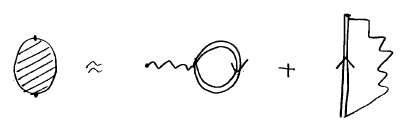
\includegraphics[width=8cm]{2-6-2.png} \label{Fig2.6.2}\end{center}
where these bold lines themselves are given by this proper selfenergy via Dyson equation,
\begin{center} 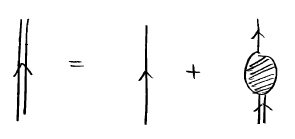
\includegraphics[width=6cm]{2-6-3.png}\label{Fig2.6.3} \end{center}
We will study these equations in details.

To this end, we will consider a spin$=\frac{1}{2}$ fermion system in a static spin-independent potential $U(\mathbf{x})$.
\[\begin{split}
\hat{H}_{0} &= \int \mathrm{d}^{3}x \  \psi_{\alpha}^{\dagger}(x)\left[ -\frac{\hbar^{2}\nabla^{2}}{2m} + U(\mathbf{x}) \right] \psi_{\alpha}(x) \\
\hat{H}_{1} &= \frac{1}{2} \int \mathrm{d}^{3}x \mathrm{d}^{3}x^{'} \ \psi_{\alpha}^{\dagger}(x) \psi_{\beta}^{\dagger}(x^{'})V(x-x^{'})\psi_{\beta}(x^{'})\psi_{\alpha}(x)
\end{split}\]
Here we assumed the spin-independent interaction potential for simplicity.

Within the self-consistent Hatree-Fock approximation, the Dyson equation is given by these two equations:
\[ \left \{ \begin{split}
G(x,y)&= G^{0}(x,y) + \int \mathrm{d}^{4}x_{1} \mathrm{d}^{4}x_{1}^{'} \ G^{0}(x,x_{1}) \Sigma^{\bigstar}% a star character
(x_{1},x_{1}^{'})G(x_{1}^{'},y)\\
\hbar \Sigma^{\bigstar}
(x_{1},x_{1}^{'})&= -\imath \delta(t_{1}-t_{1}^{'}) \times 
\left[ \delta(\mathbf{x}_{1}-\mathbf{x}_{1}^{'}) \ 2 \int \mathrm{d}^{3}x_{2} \left( \begin{split} &G(\mathbf{x}_{2},t_{2};\mathbf{x}_{2},t_{2}+0) V(\mathbf{x}_{1}-\mathbf{x}_{2}) 
\\- &G(\mathbf{x}_{1},t_{1};\mathbf{x}_{1}^{'},t_{1}+0) V(\mathbf{x}_{1}-\mathbf{x}_{1}^{'}) \end{split}\right)
\right]
\end{split}\right. \]
Where the factor $2$ comes from the spin summations.

Now, it is convenient to use a Fourier representation.
\[ \begin{split}
G(\mathbf{x},t;\mathbf{x}^{'},t^{'})&=\frac{1}{2\pi}\int \mathrm{d} \omega \mathrm{e}^{-\imath \omega (t-t^{'})} G(\mathbf{x},\mathbf{x}^{'};\omega)\\
G^{0}(\mathbf{x},t;\mathbf{x}^{'},t^{'})&=\frac{1}{2\pi}\int \mathrm{d} \omega \mathrm{e}^{-\imath \omega (t-t^{'})} G^{0}(\mathbf{x},\mathbf{x}^{'};\omega)\\
\Sigma^{\bigstar}(\mathbf{x},t;\mathbf{x}^{'},t^{'})&=
\delta(t-t^{'})\Sigma^{\bigstar}(\mathbf{x},\mathbf{x}^{'})\\
&=\frac{1}{2\pi}\int \mathrm{d} \omega \mathrm{e}^{-\imath \omega (t-t^{'})}\Sigma^{\bigstar}(\mathbf{x},\mathbf{x}^{'})
\end{split} \]
\begin{equation}
G(\mathbf{x},\mathbf{y};\omega)=G^{0}(\mathbf{x},\mathbf{y};\omega)+\int \mathrm{d}^{3}\mathbf{x}_{1} \mathrm{d}^{3}\mathbf{x}^{'}_{1} \ G^{0}(\mathbf{x},\mathbf{x}_{1};\omega) \times \Sigma^{\bigstar}(\mathbf{x}_{1},\mathbf{x}^{'}_{1})G(\mathbf{x}^{'}_{1},\mathbf{y},\omega)
\label{Eqs2.6.1}\end{equation}
\begin{equation}\begin{split}
\hbar\Sigma^{\bigstar}(\mathbf{x}_{1},\mathbf{x}^{'}_{1})
=&-\imath 2 \delta(\mathbf{x}_{1}-\mathbf{x}^{'}_{1}) \int \mathrm{d}^{3}\mathbf{x}_{2} \ V(\mathbf{x}_{1}-\mathbf{x}_{2}) \times \frac{1}{2\pi}\int \mathrm{d} \omega \mathrm{e}^{\imath \omega 0 t} G(\mathbf{x}_{2},\mathbf{x}_{2};\omega)\\
&+\imath V(\mathbf{x}_{1}-\mathbf{x}^{'}_{1}) \frac{1}{2\pi}\int \mathrm{d} \omega \mathrm{e}^{\imath \omega 0 t} G(\mathbf{x}_{1},\mathbf{x}_{1}^{'};\omega)
\end{split}\label{Eqs2.6.2}\end{equation}
Let us also introduce the orthonormal eigenfunctions of $H_{0}$.
\[ H_{0} \ \varphi_{j}^{0}(\mathbf{x}) \equiv \left[ -\frac{\hbar^{2}\nabla^{2}}{2m} + U(\mathbf{x}) \right]\varphi_{j}^{0}(\mathbf{x}) = \epsilon_{j}\varphi_{j}^{0}(\mathbf{x}) \]
In terms of  this eigenfunctions, the field operator in the interaction representation can be expanded as
\[ \left \{ \begin{split}
\psi(\mathbf{x},t) &= \sum_{j} \varphi_{j}(\mathbf{x})c_{j}\mathrm{e}^{-\imath\frac{\epsilon_{j}t}{\hbar}}\\
\psi^{\dagger}(\mathbf{x},t) &= \sum_{j} \varphi^{*}_{j}(\mathbf{x})c_{j}^{\dagger}\mathrm{e}^{+\imath\frac{\epsilon_{j}t}{\hbar}}
\end{split} \right. \]
where we used \[\mathrm{e}^{+\imath\frac{H_{0}t}{\hbar}}c_{j}\mathrm{e}^{-\imath\frac{H_{0}t}{\hbar}}=\mathrm{e}^{-\imath\frac{\epsilon_{j}t}{\hbar}}c_{j}\]
In terms of them, the non-interacting Green's function can be calculated as
\[ \begin{split}
\imath G^{0}(\mathbf{x},t;\mathbf{x}^{'},t^{'})=& \langle \Phi_{0} | \Gamma [ \psi_{I}(\mathbf{x},t) \psi_{I}^{\dagger}(\mathbf{x}^{'},t^{'}) ] | \Phi_{0} \rangle\\
=& \  \theta(t-t^{'}) \  \langle \Phi_{0} | \psi_{I}(\mathbf{x},t) \psi_{I}^{\dagger}(\mathbf{x}^{'},t^{'}) | \Phi_{0} \rangle \\
&-\theta(t^{'}-t) \  \langle \Phi_{0} | \psi_{I}^{\dagger}(\mathbf{x}^{'},t^{'}) \psi_{I}(\mathbf{x},t) | \Phi_{0} \rangle \\
=& \ \theta(t-t^{'}) \sum_{j} \varphi_{j}^{0}(\mathbf{x})\varphi_{j}^{0*}(\mathbf{x}^{'}) \mathrm{e}^{-\imath\frac{\epsilon_{j}}{\hbar}(t-t^{'})}
\times \langle \Phi_{0} | c_{j}c_{j}^{\dagger} | \Phi_{0} \rangle \\
&-\theta(t^{'}-t) \sum_{j} \varphi_{j}^{0}(\mathbf{x})\varphi_{j}^{0*}(\mathbf{x}^{'}) \mathrm{e}^{-\imath\frac{\epsilon_{j}}{\hbar}(t-t^{'})}
\times \langle \Phi_{0} | c_{j}^{\dagger}c_{j} | \Phi_{0} \rangle\\
=&\sum_{j} \varphi_{j}^{0}(\mathbf{x})\varphi_{j}^{0*}(\mathbf{x}^{'}) \mathrm{e}^{-\imath\frac{\epsilon_{j}}{\hbar}(t-t^{'})} \times \left \{ \theta(t-t^{'})\langle \Phi_{0} | c_{j}c_{j}^{\dagger} | \Phi_{0} \rangle
-\theta(t^{'}-t)\langle \Phi_{0} | c_{j}^{\dagger}c_{j} | \Phi_{0} \rangle \right \}\\
=& \sum_{j} \varphi_{j}^{0}(\mathbf{x})\varphi_{j}^{0*}(\mathbf{x}^{'}) \mathrm{e}^{-\imath\frac{\epsilon_{j}}{\hbar}(t-t^{'})} \times \left \{ \theta(t-t^{'})\theta(\epsilon_{j}^{0}-\epsilon_{F}^{0}) - \theta(t^{'}-t)\theta(-\epsilon_{j}^{0}+\epsilon_{F}^{0}) \right \}
\end{split} \]
where $\epsilon_{F}^{0}$ is the energy of the highest filled state.

The Fourier transformation leads to
\begin{equation}\label{Eqs2.6.3}
G^{0}(\mathbf{x},\mathbf{x}^{'};\omega) = \sum_{j} \varphi_{j}^{0}(\mathbf{x})\varphi_{j}^{0*}(\mathbf{x}^{'}) \times \left[
\frac{\theta(\epsilon_{j}^{0}-\epsilon_{F}^{0})}{\omega-\hbar^{-1}\epsilon_{j}^{0}+\imath\eta} +\frac{\theta(\epsilon_{F}^{0}-\epsilon_{j}^{0})}{\omega-\hbar^{-1}\epsilon_{j}^{0}-\imath\eta}
 \right]
\end{equation}
The particle density at $\mathbf{x}$ in the unperturbed ground state is estimated as
\[ \begin{split} n^{0}(\mathbf{x}) =& -\imath \  2 \ \frac{1}{2\pi} \int \mathrm{d} \omega \mathrm{e}^{\imath\omega 0 t} G^{0}(\mathbf{x},\mathbf{x};\omega)\\
=& 2 \sum_{j} |\varphi_{j}^{0}(\mathbf{x})|^{2} \theta(\epsilon_{F}^{0}-\epsilon_{j}^{0})
\end{split}\]
where the factor 2 comes from spin.

The total number of fermions is given by its spatial integral:
\[ N = \int \mathrm{d}^{3}\mathbf{x} n^{0}(\mathbf{x}) = 2 \sum_{j} \theta(\epsilon_{F}^{0}-\epsilon_{j}^{0}) \]
where we assume the normalization of $\varphi_{j}^{0}(\mathbf{x})$

These three equations(eq.(\ref{Eqs2.6.1}),eq.(\ref{Eqs2.6.2}),eq.(\ref{Eqs2.6.3})) comprise a set of coupled equations for the Green's function G.

To solve these coupled equations in favor for G, let us apply a following differential operator onto eq.(\ref{Eqs2.6.1})
\[ L_{1} = \hbar \omega + \frac{\hbar^{2}\nabla^{2}}{2m} - V(\mathbf{x})\]
If we apply this onto $G^{0}(\mathbf{x},\mathbf{y};\omega)$, we obtain the delta function in space,
\[\begin{split} L_{1} \ G^{0}(\mathbf{x},\mathbf{y};\omega) =& \sum_{j}(\hbar\omega - \epsilon_{j}^{0})\varphi_{j}^{0}(\mathbf{x})\varphi_{j}^{0*}(\mathbf{y})
 \times \left[
\frac{\theta(\epsilon_{j}^{0}-\epsilon_{F}^{0})}{\omega-\hbar^{-1}\epsilon_{j}^{0}+\imath\eta} +\frac{\theta(\epsilon_{F}^{0}-\epsilon_{j}^{0})}{\omega-\hbar^{-1}\epsilon_{j}^{0}-\imath\eta}
 \right]\\
=& \hbar \sum_{j} \varphi_{j}^{0}(\mathbf{x})\varphi_{j}^{0*}(\mathbf{y}) = \hbar \delta^{3}(\mathbf{x}-\mathbf{y})
\end{split} \]
Thus, an application of $L_{1}$ onto eq.(\ref{Eqs2.6.1}) leads to
\[ L_{1} \ G(\mathbf{x},\mathbf{y};\omega) = \hbar\delta^{3}(\mathbf{x}-\mathbf{y}) + \int \mathrm{d}^{3}\mathbf{x}_{1}^{'} 
\hbar\Sigma^{\bigstar}(\mathbf{x},\mathbf{x}_{1}^{'})G(\mathbf{x}_{1}^{'},\mathbf{y};\omega) \]
or equivalently
\begin{equation}\label{Eqs2.6.4}
\left[ \hbar\omega + \frac{\hbar^{2}\nabla^{2}_{\mathbf{x}}}{2m} - V(\mathbf{x}) \right] G(\mathbf{x},\mathbf{y};\omega) - \int \mathrm{d}^{3} \mathbf{x}^{'} \hbar \Sigma^{\bigstar}(\mathbf{x},\mathbf{x}^{'})G(\mathbf{x}^{'},\mathbf{y};\omega) = \hbar\delta^{3}(\mathbf{x}-\mathbf{y})
\end{equation}
Generally, such a linearized integral equation can be solved in terms of following set of eigenstates $\varphi_{j}(\mathbf{x})$
\begin{equation} \label{Eqs2.6.5}
 \left[ -\frac{\hbar^{2}\nabla^{2}_{\mathbf{x}}}{2m} + V(\mathbf{x}) \right]\varphi_{j}(\mathbf{x})+\int \mathrm{d}^{3} \mathbf{x}^{'} \hbar \Sigma^{\bigstar}(\mathbf{x},\mathbf{x}^{'})\varphi_{j}(\mathbf{x}^{'})=\epsilon_{j}\varphi_{j}(\mathbf{x}) \end{equation}

\[ \begin{split} iG_{\alpha\beta}(\mathbf{x},t;\mathbf{x}^{'},t^{'}) =
 \sum_{n} \{ &\theta(t-t^{'}) \mathrm{e}^{\frac{-\imath(E_{n}-E)(t-t^{'})}{\hbar}} \times \langle \Psi_{0} | \psi_{\alpha}(\mathbf{x}) | \Psi_{n} \rangle \langle \Psi_{n} | \psi_{\beta}^{\dagger}(\mathbf{x}^{'}) | \Psi_{0} \rangle  \\
- \ &\theta(t^{'}-t) \mathrm{e}^{\frac{-\imath(E_{n}-E)(t-t^{'})}{\hbar}} \times \langle \Psi_{0} | \psi_{\beta}^{\dagger}(\mathbf{x}^{'}) | \Psi_{n} \rangle \langle \Psi_{n} | \psi_{\alpha}(\mathbf{x}) | \Psi_{0} \rangle \}
\end{split} \]
\[ \begin{split} G_{\alpha\beta}(\mathbf{x},\mathbf{x}^{'};\omega) = \sum_{n} [ 
&\frac{\langle \Psi_{0} | \psi_{\alpha}(\mathbf{x}) | \Psi_{n} \rangle \langle \Psi_{n} | \psi_{\beta}^{\dagger}(\mathbf{x}^{'}) | \Psi_{0} \rangle}{\omega-\hbar^{-1}(E_{n}-E)+\imath\eta} \\
+&\frac{\langle \Psi_{0} | \psi_{\beta}^{\dagger}(\mathbf{x}^{'}) | \Psi_{n} \rangle \langle \Psi_{n} | \psi_{\alpha}(\mathbf{x}) | \Psi_{0} \rangle}{\omega-\hbar^{-1}(E_{n}-E)-\imath\eta} ]
\end{split} \]
\[ \frac{1}{2\pi} \int_{-\infty}^{+\infty} \mathrm{d}\omega G_{\alpha\beta}(\mathbf{x},\mathbf{x}^{'};\omega)\mathrm{e}^{\imath\omega 0 t} = \imath \sum_{n} \langle \Psi_{0} | \psi_{\beta}^{\dagger}(\mathbf{x}^{'}) | \Psi_{n} \rangle \langle \Psi_{n} | \psi_{\alpha}(\mathbf{x}) | \Psi_{0} \rangle \]
\[ {\left ( \imath \int_{-\infty}^{+\infty} \mathrm{d} \omega G(\mathbf{x},\mathbf{x}^{'};\omega)\mathrm{e}^{\imath \omega 0 t} \right )}^{*} = \imath \int_{-\infty}^{+\infty} \mathrm{d} \omega G(\mathbf{x}^{'},\mathbf{x};\omega)\mathrm{e}^{\imath \omega 0 t} \]
where $\hbar\Sigma^\bigstar$ play role of a static but no-local potential.

Since $\Sigma^\bigstar$ is hermitian,\[\Sigma^{\bigstar*}(\mathbf{x},\mathbf{x}^{'}) = \Sigma^\bigstar(\mathbf{x}^{'},\mathbf{x}) \]
$\{\varphi_{j}\}$ comprises complete set of orthonormal eigenfunctions with
\[ \sum_{j} \varphi_{j}(\mathbf{x})\varphi_{j}^{*}(\mathbf{x}^{'}) = \delta^{3}(\mathbf{x}-\mathbf{x}^{'}) \]
\[ \int \mathrm{d}^3 \mathbf{x} \varphi_j^*(\mathbf{x})\varphi_m(\mathbf{x}) = \delta_{jm} \]
and $\epsilon_j$ is real.

In terms of this eigenstates, the Green's function satisfying eq.(\ref{Eqs2.6.4}) is roughly given in a following form:
\[ G(\mathbf{x},\mathbf{y};\omega) \sim \sum_j \varphi_j(\mathbf{x})\varphi_j^*(\mathbf{y}) \cdot \frac{1}{\omega-\hbar^{-1}\epsilon_j} \]


According to eq.(\ref{Eqs2.3.2.a}), the particle density and total number of the particles are given by the frequency integral of this Green's function.
\[ n(\mathbf{x}) = - \imath \ 2 \cdot \frac{1}{2\pi} \int_{-\infty}^{+\infty} \mathrm{d} \omega \mathrm{e}^{\imath \omega  0 t} G(\mathbf{x},\mathbf{x};\omega) \]
\[ N = -\imath \ 2 \cdot \frac{1}{2\pi} \int \mathrm{d}^3 \mathbf{x} \int_{-\infty}^{+\infty} \mathrm{d} \omega \mathrm{e}^{\imath \omega  0 t} G(\mathbf{x},\mathbf{x};\omega) \]


But, since the perturbation $\hat{H}_1$ conserves the total number of particles, the number of particles thus calculated should be equal to the number of particles in the unperturbed ground state. To make it possible, the denominator in the r.h.s. of this equation should acquire an infinitesimally small imaginary part like this:
\begin{equation}\label{Eqs2.6.6}
G(\mathbf{x},\mathbf{y};\omega) = \sum_j \varphi_j(\mathbf{x}) \varphi_j^* (\mathbf{y})
\left[ \frac{\theta(\epsilon_j - \epsilon_F)}{\omega - \hbar^{-1}\epsilon_j + \imath \eta} + \frac{\theta(\epsilon_F - \epsilon_j)}{\omega - \hbar^{-1}\epsilon_j - \imath \eta} \right]   \quad (\eta > 0)
\end{equation}
$\epsilon_F $ here denote the energy of the highest filled state of these orthonormal eigenstates, which satisfies
\[ \sum_j \theta(\epsilon_F - \epsilon_j) = N \equiv \sum_j \theta(\epsilon_F^0 - \epsilon_j^0) \]
substituting this solution back into eq.(\ref{Eqs2.6.2}), we obtain the self-energy itself, which is given by these orthonormal eigenstates.
\begin{equation}\label{Eqs2.6.7} \begin{split}
 \hbar \Sigma^\bigstar (\mathbf{x}_1,\mathbf{x}_1^{'}) =
& 2 \ \delta(\mathbf{x}_1 - \mathbf{x}_1^{'}) \int \mathrm{d}^3 \mathbf{x}_2 V(\mathbf{x}_1 - \mathbf{x}_2) \times \sum_j |\varphi_j(\mathbf{x}_2)|^2 \theta(\epsilon_F - \epsilon_j) \\
&- V(\mathbf{x}_1 - \mathbf{x}_1^{'}) \sum_j \varphi_j (\mathbf{x}_1) \varphi_j^* (\mathbf{x}_1^{'}) \theta(\epsilon_F - \epsilon_j) \\
=& \delta(\mathbf{x}_1 - \mathbf{x}_1^{'}) \int \mathrm{d}^3 \mathbf{x}_2 V(\mathbf{x}_1 - \mathbf{x}_2) n(\mathbf{x}_2) \quad \text{(Fock term)}\\
&- V(\mathbf{x}_1 - \mathbf{x}_1^{'})\sum_j \varphi_j(\mathbf{x}_1)\varphi_j^*(\mathbf{x}_1^{'})\theta(\epsilon_F - \epsilon_j) \quad \text{(Hartree term)}
\end{split}\end{equation}
Within this HF approximation, the self-energy consists of two terms. One is a local term propotional to particle density, and the other is non-local exchange term. These two are often called as Hartree term and Fock term respectively.

To summarize, eq.(\ref{Eqs2.6.5}) and eq.(\ref{Eqs2.6.7}) comprise a self-consistent equations for the orthonormal eigenstates $\varphi_j$ and its eigenvalue $\epsilon_j$.

Namely, once  $\varphi_j$ and $\epsilon_j$ are given, the self-energy $\Sigma^\bigstar$ are calculated by eq.(\ref{Eqs2.6.7}). In terms of this self-energy, the orthonormal eigenstates $\varphi_j$ and $\epsilon_j$ are recalculated. This process is repeated, until a self-consistent solution for \{$\varphi_j$\} and \{$\epsilon_j$\} is obtained.

Once the self-consistent solution is obtained, we can calculate Green's function from eq.(\ref{Eqs2.6.6}), from which we can calculate various physical quantities such as ground state energy and ground state expectation value of single particle operators.
\begin{center}-------------------\end{center}

This is all about the Hartree-Fock approximation, which is quite commonly used in condensed matter physics research.

In the following two sections, I will describe two other standard approximation scheme commonly used in the contemporary research.

\section{Imperfect Fermi Gas}%wsz 2-7
The first system considered is a dilute Fermi gas with strong short-range repulsive interaction, which is somtimes called as ``imperfect Fermi gas".

We assume that the repulsive interaction is s-wave like, so that the potential depends only on a spatial distance between two particles.

To be specific, we assume that the repulsive interaction is described by a square-well shape potential.
\begin{center} \label{Fig2.7.1} 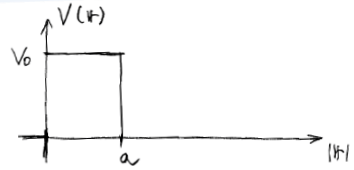
\includegraphics[width=6cm]{2-7-1.png}
\end{center}
where positive $V_0$ means repulsive and ``$a$" represents an interaction range.

``strong short-range repulsive interaction" means that ``$V_0$" will be taken to be sufficiently large, but ``$a$" will be taken to be small.
\[ \left \{ \begin{split} V_0 &\rightarrow \text{large} \\ a &\rightarrow \text{small} \end{split} \right. \]

For the kinetic energy part, we simply assume the free electron Hamiltonian
\[H_0 = \sum_\alpha \int \mathrm{d}^3 \mathbf{x} \psi_\alpha^\dagger (\mathbf{x}) \left[-\frac{\hbar^2\nabla^2_{\mathbf{x}}}{2m}\right]\psi_\alpha(\mathbf{x})\]
whose dispersion take a parabolic form.
\begin{center} \label{Fig2.7.2} 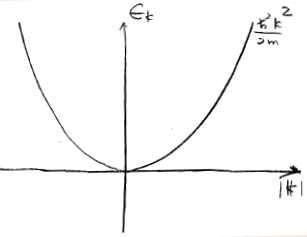
\includegraphics[width=3cm]{2-7-2.png} \end{center}

``dilute Fermi gas" means that the chemical potential is chosen so that the Fermi momentum is sufficiently small. $$k_F \rightarrow \text{small}$$

Now $k_F a$ comprises a dimensionless quantity. The natural coupling constant for ``imperfect Fermi gas" is ``$k_F a$". Namely, we are going to analyize the ``imperfect Fermi gas" by treating ``$k_F a$" as a small parameter. Thereby, physical quantities such as ground state energy, chemical potential and quasi-particle spectrum are calculated, perturbatively in small $k_F a$.
\[ \text{e.g.)} \quad \frac{E}{N} = \frac{\hbar^2 k_F^2}{2m} \left[ A + B(k_F a) + C{(k_F a)}^2 + \ldots \right] \]

To do this perturbation expansion, systematically, let us begin with the 2nd order contribution to the proper self energy.

According to eq.(\ref{Eqs2.6.4}), the 2nd order contribution can be enumerated as follows:
\begin{center}\label{Fig2.7.3} 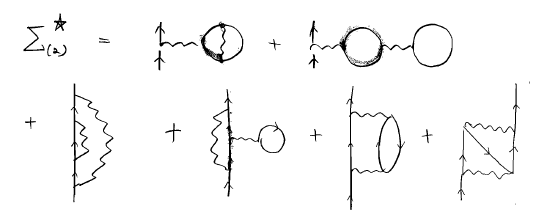
\includegraphics[width=8cm]{2-7-3.png} \end{center}

For the uniform electron gas case, these four term exactly reduce to zero.
\begin{center}-----------------------------\end{center}

\begin{wrapfigure}{l}{3.5cm}
\label{Fig2.7.4} \includegraphics[width=3cm]{2-7-4.png}
\end{wrapfigure}
For example, consider this diagram.

The self energy part can be calculated as this.
\[ \begin{split} & {\left(\frac{\imath}{\hbar} \right)}^2 \frac{1}{\left( 2\pi \right)^8} \int \mathrm{d}^3 \mathbf{q} \int \mathrm{d}\epsilon \int \mathrm{d}^3 \mathbf{q}^{'} \int \mathrm{d} \epsilon^{'} \\
& \  \times \left\{ V(\mathbf{q}-\mathbf{q}^{'})V(\mathbf{k}-\mathbf{q})\mathrm{e}^{\imath \epsilon^{'} 0 t} G_0(\mathbf{q}^{'},\epsilon^{'}) \times \left[ G_0(\mathbf{q},\epsilon) \right]^2 \right \} \end{split} \]

where
\[ G_0(\mathbf{q},\epsilon) \equiv \frac{\theta(|\mathbf{q}|-k_F)}{\epsilon - \epsilon_{\mathbf{q}}+\imath \eta} + \frac{\theta(k_F-|\mathbf{q}|)}{\epsilon - \epsilon_{\mathbf{q}}-\imath \eta} \]

Putting this into here, this part becomes like this:
\[ \int \frac{\mathrm{d}\epsilon^{'}}{2\pi} \left[ \frac{\theta(|\mathbf{q}|-k_F)}{\epsilon^{'} - \epsilon_{\mathbf{q}^{'}}+\imath \eta} + \frac{\theta(k_F-|\mathbf{q}|)}{\epsilon^{'} - \epsilon_{\mathbf{q}^{'}}-\imath \eta} \right]^2 \]

Since $$\theta(|\mathbf{q}|-k_F)\theta(k_F-|\mathbf{q}|) = 0$$

 the cross term vanishes, so that we have
\[ \int \frac{\mathrm{d}\epsilon^{'}}{2\pi} \left[ \frac{\theta(|\mathbf{q}|-k_F)}{\left(\epsilon^{'} - \epsilon_{\mathbf{q}^{'}}+\imath \eta\right)^2} + \frac{\theta(k_F-|\mathbf{q}|)}{\left(\epsilon^{'} - \epsilon_{\mathbf{q}^{'}}-\imath \eta\right)^2} \right] \]

Now we can integrate this, by closing the contour either in the upper half plane or in the lower half plane(By using the method of contour integration).

But, since both of these two are the second order pole, the contour integration always reduce to zero, irrespective of whether the integration is carried out in the upper--half plane or in the lower--half plane.

Therefore, this contribution always reduce to zero. Similarly, we can immediately see that all of these also reduce to zero, because these parts give the same integration as this.

\begin{wrapfigure}[8]{l}{4.5cm}
\label{Fig2.7.5} \includegraphics[width=4cm]{2-7-5.png}
\end{wrapfigure}
Thus, we have only to calculate these two contributions,
\[ \begin{split} &- \left( \frac{\imath}{\hbar}\right)^2 \frac{1}{\left( 2\pi \right)^8} \int \mathrm{d}^3 \mathbf{q} \int \mathrm{d}\epsilon \int \mathrm{d}^3 \mathbf{q}^{'} \int \mathrm{d} \epsilon^{'} \\
&\times \left\{ \ V^2(\mathbf{q})G_0(\mathbf{k}-\mathbf{q},\omega-\epsilon) \times G_0(\mathbf{q} + \mathbf{q}^{'}, \epsilon + \epsilon^{'}) G_0(\mathbf{q}^{'},\mathbf{\epsilon}^{'}) \right\} \end{split} \]

%Let me try this first.

Let me first integrate over these internal frequencies by using the method of contour integration.
\[ \begin{split} \int \frac{\mathrm{d}\epsilon}{2\pi} \int \frac{\mathrm{d}\epsilon^{'}}{2\pi}
&\left[ \frac{\theta(|\mathbf{k}-\mathbf{q}|-k_F)}{\omega - \epsilon - \epsilon_{\mathbf{k}-\mathbf{q}}+\imath \eta} + \frac{\theta(k_F-|\mathbf{k}-\mathbf{q}|)}{\omega - \epsilon - \epsilon_{\mathbf{k}-\mathbf{q}}-\imath \eta} \right] \\
& \times \left[ \frac{\theta(|\mathbf{q}+\mathbf{q}^{'}|-k_F)}{\epsilon + \epsilon^{'} - \epsilon_{\mathbf{q}+\mathbf{q}^{'}}+\imath \eta} + \frac{ \theta(k_F-|\mathbf{q}+\mathbf{q}^{'}|)}{\epsilon + \epsilon^{'} - \epsilon_{\mathbf{q}+\mathbf{q}^{'}}-\imath \eta} \right] \\
& \times \left[ \frac{\theta(|\mathbf{q}^{'}|-k_F)}{\epsilon^{'} - \epsilon_{\mathbf{q}^{'}}+\imath \eta} + \frac{\theta(k_F-|\mathbf{q}^{'}|)}{\epsilon^{'} - \epsilon_{\mathbf{q}^{'}}-\imath \eta} \right]
\end{split} \]
I will first integrate over $\epsilon$, whose integrand is the product between these two:
\[\left[ \frac{\theta(|\mathbf{k}-\mathbf{q}|-k_F)}{\omega - \epsilon - \epsilon_{\mathbf{k}-\mathbf{q}}+\imath \eta} + \frac{\theta(k_F-|\mathbf{k}-\mathbf{q}|)}{\omega - \epsilon - \epsilon_{\mathbf{k}-\mathbf{q}}-\imath \eta} \right]
\times \left[ \frac{\theta(|\mathbf{q}+\mathbf{q}^{'}|-k_F)}{\epsilon + \epsilon^{'} - \epsilon_{\mathbf{q}+\mathbf{q}^{'}}+\imath \eta} + \frac{ \theta(k_F-|\mathbf{q}+\mathbf{q}^{'}|)}{\epsilon + \epsilon^{'} - \epsilon_{\mathbf{q}+\mathbf{q}^{'}}-\imath \eta} \right] \]

From this product, we have four terms.

But these two reduce to zero, when the contour integration over $\epsilon$ is carried out.
\[ \frac{\ldots}{\omega - \epsilon - \epsilon_{\mathbf{k}-\mathbf{q}} \pm \imath \eta} \cdot \frac{ \ldots}{\epsilon + \epsilon^{'} - \epsilon_{\mathbf{q}+\mathbf{q}^{'}} \mp \imath \eta} \]

Namely these two have a pole in the upper half plane, while these two have a pole in the lower half plane. Thus, for this term, we can close the contour in the lower half plane, while for this term, we can close the contour in the upper half plane, which reduce them to zero under the integration.

On the one hand, these combinations always have a pole both in the upper half plane and in the lower half plane.
\[ \frac{\ldots}{\omega - \epsilon - \epsilon_{\mathbf{k}-\mathbf{q}} \pm \imath \eta} \cdot \frac{ \ldots}{\epsilon + \epsilon^{'} - \epsilon_{\mathbf{q}+\mathbf{q}^{'}} \pm \imath \eta} \]

Thus, irrespective of how the contour is closed, these two combinations give finite contribution.
\[\begin{split} \int \frac{\mathrm{d} \epsilon}{2\pi}
&\left \{ \frac{\theta(|\mathbf{k}-\mathbf{q}|-k_F)}{\omega - \epsilon - \epsilon_{\mathbf{k}-\mathbf{q}} + \imath \eta} \cdot \frac{ \theta(|\mathbf{q}+\mathbf{q}^{'}|-k_F)}{\epsilon + \epsilon^{'} - \epsilon_{\mathbf{q}+\mathbf{q}^{'}} + \imath \eta}
+ \frac{\theta(k_F-|\mathbf{k}-\mathbf{q}|)}{\omega - \epsilon - \epsilon_{\mathbf{k}-\mathbf{q}} - \imath \eta} \cdot \frac{ \theta(k_F-|\mathbf{q}+\mathbf{q}^{'}|)}{\epsilon + \epsilon^{'} - \epsilon_{\mathbf{q}+\mathbf{q}^{'}} - \imath \eta} \right \}\\
& = -\imath \cdot \frac{\theta(|\mathbf{k}-\mathbf{q}|-k_F)\theta(|\mathbf{q}+\mathbf{q}^{'}|-k_F)}{\omega - \epsilon_{\mathbf{k}-\mathbf{q}} + \epsilon^{'} - \epsilon_{\mathbf{q}+\mathbf{q}^{'}} + 2 \imath \eta }
+\imath \cdot \frac{\theta(k_F-|\mathbf{k}-\mathbf{q}|)\theta(k_F-|\mathbf{q}+\mathbf{q}^{'}|)}{\omega - \epsilon_{\mathbf{k}-\mathbf{q}} + \epsilon^{'} - \epsilon_{\mathbf{q}+\mathbf{q}^{'}} - 2 \imath \eta }
\end{split} \]

Let me next integrate over $\epsilon^{'}$, by subtituting this into here. From this product, we again have four terms.

Now these two have a pole in the upper half plane, while these two have a pole in the lower half plane. Due to the same reason, only these two combinations give us a finite contribution.
\[\begin{split}  (-\imath) \{
&\int \frac{\mathrm{d}\epsilon^{'}}{2\pi} \  \frac{\theta(|\mathbf{k}-\mathbf{q}|-k_F)\theta(|\mathbf{q}+\mathbf{q}^{'}|-k_F)}{\epsilon^{'} + \omega - \epsilon_{\mathbf{k}-\mathbf{q}} - \epsilon_{\mathbf{q}+\mathbf{q}^{'}} + 2 \imath \eta }
\cdot \frac{\theta(k_F-|\mathbf{q}^{'}|)}{\epsilon^{'}-\epsilon_{\mathbf{q}^{'}}-\imath \eta} \\
&- \int \frac{\mathrm{d}\epsilon^{'}}{2\pi} \ \frac{\theta(k_F-|\mathbf{k}-\mathbf{q}|)\theta(k_F-|\mathbf{q}+\mathbf{q}^{'}|)}{\epsilon^{'} + \omega - \epsilon_{\mathbf{k}-\mathbf{q}} - \epsilon_{\mathbf{q}+\mathbf{q}^{'}} - 2 \imath \eta }
\cdot \frac{\theta(|\mathbf{q}^{'}|-k_F)}{\epsilon^{'}-\epsilon_{\mathbf{q}^{'}}+\imath \eta} \} \\
=(-\imath) \{
&\imath \frac{\theta(|\mathbf{k}-\mathbf{q}|-k_F)\theta(|\mathbf{q}+\mathbf{q}^{'}|-k_F)\theta(k_F-|\mathbf{q}^{'}|)}{\omega - \epsilon_{\mathbf{k}-\mathbf{q}}-\epsilon_{\mathbf{q}+\mathbf{q}^{'}}+\epsilon_{\mathbf{q}^{'}}+3\imath \eta}\\
&+\imath \frac{\theta(k_F-|\mathbf{k}-\mathbf{q}|)\theta(k_F-|\mathbf{q}+\mathbf{q}^{'}|)\theta(|\mathbf{q}^{'}|-k_F)}{\omega - \epsilon_{\mathbf{k}-\mathbf{q}}-\epsilon_{\mathbf{q}+\mathbf{q}^{'}}+\epsilon_{\mathbf{q}^{'}}-3\imath \eta}
\}
 \end{split}\]

\begin{wrapfigure}[4]{l}{3.5cm}
\label{Fig2.7.6} \includegraphics[width=3cm]{2-7-6.png}
\end{wrapfigure}

By substituting this into the original expression we obtain this:
\begin{equation} \label{Eqs2.7.1} \begin{split}
= & \frac{1}{\hbar^2} \int \frac{\mathrm{d}\mathbf{q}}{\left( 2\pi \right)^3} \int \frac{\mathrm{d}\mathbf{q}^{'}}{\left( 2\pi \right)^3} \\
& \times V^2(\mathbf{q}) \{
\frac{\theta(|\mathbf{k}-\mathbf{q}|-k_F)\theta(|\mathbf{q}+\mathbf{q}^{'}|-k_F)\theta(k_F-|\mathbf{q}^{'}|)}{\omega - \epsilon_{\mathbf{k}-\mathbf{q}}-\epsilon_{\mathbf{q}+\mathbf{q}^{'}}+\epsilon_{\mathbf{q}^{'}}}
\\
&+\frac{\theta(k_F-|\mathbf{k}-\mathbf{q}|)\theta(k_F-|\mathbf{q}+\mathbf{q}^{'}|)\theta(|\mathbf{q}^{'}|-k_F)}{\omega - \epsilon_{\mathbf{k}-\mathbf{q}}-\epsilon_{\mathbf{q}+\mathbf{q}^{'}}+\epsilon_{\mathbf{q}^{'}}}
\} \end{split}\end{equation}

\begin{wrapfigure}[4]{l}{3.5cm}
\label{Fig2.7.7} \includegraphics[width=3cm]{2-7-7.png}
\end{wrapfigure}
Similarly we can calculate the other 2nd order contribution to the proper self-energy.
\[ \begin{split} & \left(\frac{\imath}{\hbar}\right)^2 \frac{1}{(2\pi)^8} \int \mathrm{d}^3 \mathbf{q} \int \mathrm{d} \epsilon \int \mathrm{d}^3 \mathbf{q}^{'} \int \mathrm{d} \epsilon^{'}  \\
& \times \left\{ V(\mathbf{q}^{'})V(-\mathbf{q} + \mathbf{q}^{'}+\mathbf{k})
\times G_0(\mathbf{q}-\mathbf{q}^{'},\epsilon-\epsilon^{'})G_0(\mathbf{q},\epsilon)G_0(\mathbf{q}^{'}+\mathbf{k},\epsilon^{'}+\omega) \right\} \end{split}\]
\begin{center}---------------------------------------------\end{center}
\[ \begin{split}
&\quad \begin{split} \int \frac{\mathrm{d}\epsilon}{2\pi}\int \frac{\mathrm{d}\epsilon^{'}}{2\pi}
& \left[ \frac{\theta(|\mathbf{q}-\mathbf{q}^{'}|-k_F)}{\epsilon - \epsilon^{'}-\epsilon_{\mathbf{q}-\mathbf{q}^{'}}+\imath\eta} + \frac{\theta(k_F-|\mathbf{q}-\mathbf{q}^{'}|)}{\epsilon - \epsilon^{'}-\epsilon_{\mathbf{q}-\mathbf{q}^{'}}-\imath\eta} \right] \\
& \times \left[ \frac{\theta(|\mathbf{q}|-k_F)}{\epsilon -\epsilon_{\mathbf{q}}+\imath\eta} + \frac{\theta(k_F-|\mathbf{q}|)}{\epsilon -\epsilon_{\mathbf{q}}-\imath\eta} \right] \\
& \times \left[ \frac{\theta(|\mathbf{q}^{'}+\mathbf{k}|-k_F)}{\epsilon^{'}+\omega -\epsilon_{\mathbf{q}^{'}+\mathbf{k}}+\imath\eta} + \frac{\theta(k_F-|\mathbf{q}^{'}+\mathbf{k}|)}{\epsilon^{'}+\omega -\epsilon_{\mathbf{q}^{'}+\mathbf{k}}-\imath\eta} \right]
\end{split}
\\
& \begin{split}=
\int \frac{\mathrm{d}\epsilon}{2\pi} \{ & \frac{\theta(|\mathbf{q}|-k_F)}{\epsilon -\epsilon_{\mathbf{q}}+\imath\eta} + \frac{\theta(k_F-|\mathbf{q}|)}{\epsilon -\epsilon_{\mathbf{q}}-\imath\eta} \} \\
\times(-\imath)\{ & \frac{\theta(|\mathbf{q}-\mathbf{q}^{'}|-k_F)\theta(|\mathbf{q}^{'}+\mathbf{k}|-k_F)}{\epsilon + \omega - \epsilon_{\mathbf{q}^{'}+\mathbf{k}} - \epsilon_{\mathbf{q}-\mathbf{q}^{'}} + 2 \imath \eta }\\
&+\frac{\theta(k_F-|\mathbf{q}-\mathbf{q}^{'}|)\theta(k_F-|\mathbf{q}^{'}+\mathbf{k}|)}{\epsilon + \omega - \epsilon_{\mathbf{q}^{'}+\mathbf{k}} - \epsilon_{\mathbf{q}-\mathbf{q}^{'}} - 2 \imath \eta }
\}
\end{split}\\
& \begin{split}=  \ - \{&
\frac{\theta(|\mathbf{q}|-k_F)\theta(k_F-|\mathbf{q}-\mathbf{q}^{'}|)\theta(k_F-|\mathbf{q}^{'}+\mathbf{k}|)}{\omega+\epsilon_{\mathbf{q}} - \epsilon_{\mathbf{q}^{'}+\mathbf{k}}-\epsilon_{\mathbf{q}-\mathbf{q}^{'}}-3\imath \eta}\\
&+\frac{\theta(k_F-|\mathbf{q}|)\theta(|\mathbf{q}-\mathbf{q}^{'}|-k_F)\theta(|\mathbf{q}^{'}+\mathbf{k}|-k_F)}{\omega+\epsilon_{\mathbf{q}} - \epsilon_{\mathbf{q}^{'}+\mathbf{k}}-\epsilon_{\mathbf{q}-\mathbf{q}^{'}}+3\imath \eta} \} \end{split}
\end{split} \]

%\begin{wrapfigure}{l}{3.5cm}
%\label{Fig2.7.8} \includegraphics[width=3cm]{2-7-8.png}
%\end{wrapfigure}
\begin{center}---------------------------------------------\end{center}
\begin{equation} \label{Eqs2.7.2} \begin{split}
\rightarrow + \int \frac{\mathrm{d}^3 \mathbf{q}}{(2\pi)^3}\int \frac{\mathrm{d}^3 \mathbf{q}^{'}}{(2\pi)^3} \times [ &\frac{\theta(k_F-|\mathbf{q}|)\theta(|\mathbf{q}-\mathbf{q}^{'}|-k_F)\theta(|\mathbf{q}^{'}+\mathbf{k}|-k_F)}{\omega+\epsilon_{\mathbf{q}} - \epsilon_{\mathbf{q}^{'}+\mathbf{k}}-\epsilon_{\mathbf{q}-\mathbf{q}^{'}}} \\
& \ + \frac{\theta(|\mathbf{q}|-k_F)\theta(k_F-|\mathbf{q}-\mathbf{q}^{'}|)\theta(k_F-|\mathbf{q}^{'}+\mathbf{k}|)}{\omega+\epsilon_{\mathbf{q}} - \epsilon_{\mathbf{q}^{'}+\mathbf{k}}-\epsilon_{\mathbf{q}-\mathbf{q}^{'}}} ]
\end{split} \end{equation}

\begin{center}---------------------\end{center}

Observing these two expressions, notice that the integrants always contain the step function
\[ \theta(x) = \begin{cases} 1 & x > 0\\ 0 & x < 0 \end{cases} \]

which is nothing but the fermion distribution function at the zero temperature. Thus, this step function represents whether the intermediate state is particle-like excited state or hole-like excited state.

Due to this fermi distribution function, the momentum integral regions associated with these internal lines are highly restricted in the low density limit.

For example, this step function $\theta(k_F - |\mathbf{q}|)$ restrict this momentum ($\mathbf{q}$) integral within a small sphere whose radius is $k_F$. While these two step function $\theta(k_F-|\mathbf{q}-\mathbf{q}^{'}|)\theta(k_F-|\mathbf{q}^{'}+\mathbf{k}|)$ restrict these two momentum ($\mathbf{q}$ and $\mathbf{q}^{'}$) variables within a sphere of radius $k_F$.%

Accordingly, in the low density limit, the first term vanishes on the order of $k_F$, while the 2nd term vanishes on the order of $k_F^2$. Thus, we can regard that the first term dominates over the 2nd term, and these two contribution gives a quantity of the order of $k_F a$ in the low--density limit.

When generalizing this argument into higher order contribution to the proper self energy, we see that the leading order contribution in the low density limit comes only from the so--called ladder--type diagrams depicted here:

\begin{center}
\includegraphics[width=8cm]{2-7-9.png}\label{Fig2.7.9}
\begin{equation} \label{Eqs2.7.3}\end{equation}
\end{center}

A basic feature of these ladder--type diagrams is as follows.

When all the interaction lines are put along the horizontal direction, any ladder--type diagrams contain \underline{only one} internal line which runs in the reverse direction to the other internal lines.

In these diagrams, \underline{these} are the ones which run in the reverse direction.

\begin{wrapfigure}[6]{l}{3.5cm}
\label{Fig2.7.10} \includegraphics[width=3cm]{2-7-10.png}
\end{wrapfigure}
Due to this feature, the integrant of these diagram contains $(2n-1)$--numbers of fermi distribution function for particle times one fermi distribution function for hole.
\[ \begin{split}
= &\int \frac{\mathrm{d}^3 \mathbf{q}_1}{(2\pi)^3} \int \frac{\mathrm{d}^3 \mathbf{q}_2}{(2\pi)^3} \ldots \int \frac{\mathrm{d}^3 \mathbf{q}_n}{(2\pi)^3} V^n \\
& \times \{  \frac{
\begin{matrix} (2n-1)\text{number for particle lines} \\ \overbrace{ \theta(|\mathbf{q}_1|-k_F)\theta(|\mathbf{q}_2|-k_F)\ldots\theta(|\mathbf{q}_n|-k_F) } \end{matrix}
\begin{matrix} (1) \text{hole line} \\ \overbrace{ \theta(k_F-|-\mathbf{k}+\mathbf{q}_{n-1}+\mathbf{q}_n|)} \end{matrix}}{\text{(energy denominator)}}\\
& + o((k_F a)^2) \}
\end{split} \]

Any Feynman diagrams other than these ladder--type diagram contain at least two internal lines which run in the reverse direction to the other internal lines. Therefore, their leading order term always contain at least two hole lines, so that they are at most the 2nd order of $k_F a$.

For example, consider a following 3rd order perturbation to the proper self energy term.
\begin{center}
\label{Fig2.7.11} \includegraphics[width=6cm]{2-7-11.png}
\end{center}

When all the interaction lines are put in the horizontal way, this Feynman diagram contain two internal lines which run in the reverse direction to the other.
\begin{center}
\label{Fig2.7.12} \includegraphics[width=6cm]{2-7-12.png}
\end{center}

\[ \begin{split}
-&\left(\frac{\imath}{\hbar}\right)^3 \ \frac{1}{(2\pi)^{12}} \int \mathrm{d}^3 \mathbf{q}_1 \int \mathrm{d} \epsilon_1 \int \mathrm{d}^3 \mathbf{q}_2 \int \mathrm{d} \epsilon_2 \int \mathrm{d}^3 \mathbf{q}_3 \int \mathrm{d} \epsilon_3 \\
&\times V(\mathbf{k}-\mathbf{q}_1)V(\mathbf{q}_1-\mathbf{q}_2)V(\mathbf{q}_2-\mathbf{k})\\
&\times G_0(\mathbf{q}_1,\epsilon_1)G_0(\mathbf{q}_2,\epsilon_2)G_0(\mathbf{q}_3,\epsilon_3)\\
&\times G_0(\mathbf{q}_3-\mathbf{q}_1+\mathbf{q}_2,\epsilon_3-\epsilon_1+\epsilon_2)G_0(\mathbf{q}_3-\mathbf{q}_1+\mathbf{k},\epsilon_3-\epsilon_1+\omega)
\end{split} \]
\begin{center}---------------------------------------------\end{center}
\[ \begin{split} &\int \frac{\mathrm{d}\epsilon_1}{2\pi} \int \frac{\mathrm{d}\epsilon_2}{2\pi} \int \frac{\mathrm{d}\epsilon_3}{2\pi}\left[ \frac{\theta(|\mathbf{q}_1|-k_F)}{\epsilon_1-\epsilon_{\mathbf{q}_1}+\imath \eta} + \frac{\theta(k_F-|\mathbf{q}_1|)}{\epsilon_1-\epsilon_{\mathbf{q}_1}-\imath \eta} \right] \\
& \times \left[ \frac{\theta(|\mathbf{q}_2|-k_F)}{\epsilon_2-\epsilon_{\mathbf{q}_2}+\imath \eta} + \frac{\theta(k_F-|\mathbf{q}_2|)}{\epsilon_2-\epsilon_{\mathbf{q}_2}-\imath \eta} \right] \times \left[ \frac{\theta(|\mathbf{q}_3|-k_F)}{\epsilon_3-\epsilon_{\mathbf{q}_3}+\imath \eta} + \frac{\theta(k_F-|\mathbf{q}_3|)}{\epsilon_3-\epsilon_{\mathbf{q}_3}-\imath \eta} \right] \\
& \times \left[ \frac{\theta(|\mathbf{q}_3-\mathbf{q}_1+\mathbf{q}_2|-k_F)}{\epsilon_3-\epsilon_1+\epsilon_2-\epsilon_{\mathbf{q}_3-\mathbf{q}_1+\mathbf{q}_2}+\imath \eta} + \frac{\theta(k_F-|\mathbf{q}_3-\mathbf{q}_1+\mathbf{q}_2|)}{\epsilon_3-\epsilon_1+\epsilon_2-\epsilon_{\mathbf{q}_3-\mathbf{q}_1+\mathbf{q}_2}-\imath \eta} \right]\\
& \times \left[ \frac{\theta(|\mathbf{q}_3-\mathbf{q}_1+\mathbf{k}|-k_F)}{\epsilon_3-\epsilon_1+\omega-\epsilon_{\mathbf{q}_3-\mathbf{q}_1+\mathbf{k}}+\imath \eta} + \frac{\theta(k_F-|\mathbf{q}_3-\mathbf{q}_1+\mathbf{k}|)}{\epsilon_3-\epsilon_1+\omega-\epsilon_{\mathbf{q}_3-\mathbf{q}_1+\mathbf{k}}-\imath \eta} \right]\\
=& \imath \int \frac{\mathrm{d}\epsilon_1}{2\pi} \int \frac{\mathrm{d}\epsilon_3}{2\pi} \left[ \frac{\theta(|\mathbf{q}_3-\mathbf{q}_1+\mathbf{q}_2|-k_F)\theta(k_F-|\mathbf{q}_2|)}{\epsilon_3-\epsilon_1+\epsilon_{\mathbf{q}_2}-\epsilon_{\mathbf{q}_3-\mathbf{q}_1+\mathbf{q}_2}+2\imath \eta} \right. \\
& \left. - \frac{\theta(k_F-|\mathbf{q}_3-\mathbf{q}_1+\mathbf{q}_2|)\theta(|\mathbf{q}_2|-k_F)}{\epsilon_3-\epsilon_1+\epsilon_{\mathbf{q}_2}-\epsilon_{\mathbf{q}_3-\mathbf{q}_1+\mathbf{q}_2}-2\imath \eta} \right] \times \left[ \ldots \right]
\end{split} \]
%gap
\[ \begin{split} \xlongequal[\mathbf{q}_3-\mathbf{q}_2 \rightarrow \mathbf{q}_3]{\epsilon_3-\epsilon_1 \rightarrow \epsilon_3} &
\imath \int \frac{\mathrm{d}\epsilon_1}{2\pi} \int \frac{\mathrm{d}\epsilon_3}{2\pi}
\left[ \frac{\theta(|\mathbf{q}_3+\mathbf{q}_2|-k_F)\theta(k_F-|\mathbf{q}_2|)}{\epsilon_3+\epsilon_{\mathbf{q}_2}-\epsilon_{\mathbf{q}_3+\mathbf{q}_2}+2\imath \eta} \right. \\
& \left. - \frac{\theta(k_F-|\mathbf{q}_3+\mathbf{q}_2|)\theta(|\mathbf{q}_2|-k_F)}{\epsilon_3+\epsilon_{\mathbf{q}_2}-\epsilon_{\mathbf{q}_3+\mathbf{q}_2}-2\imath \eta} \right] \\
& \times \left[ \frac{\theta(|\mathbf{q}_1|-k_F)}{\epsilon_1-\epsilon_{\mathbf{q}_1}+\imath \eta} + \frac{\theta(k_F-|\mathbf{q}_1|)}{\epsilon_1-\epsilon_{\mathbf{q}_1}-\imath \eta} \right]\\
& \times \left[ \frac{\theta(|\mathbf{q}_3+\mathbf{k}|-k_F)}{\epsilon_3+\omega-\epsilon_{\mathbf{q}_3+\mathbf{k}}+\imath \eta} + \frac{\theta(k_F-|\mathbf{q}_3+\mathbf{k}|)}{\epsilon_3+\omega-\epsilon_{\mathbf{q}_3+\mathbf{k}}-\imath \eta} \right]\\
& \times \left[ \frac{\theta(|\mathbf{q}_3+\mathbf{q}_1|-k_F)}{\epsilon_3+\epsilon_1-\epsilon_{\mathbf{q}_3+\mathbf{q}_1}+\imath \eta} + \frac{\theta(k_F-|\mathbf{q}_3+\mathbf{q}_1|)}{\epsilon_3+\epsilon_1-\epsilon_{\mathbf{q}_3+\mathbf{q}_1}-\imath \eta} \right] \\
=& (\imath)^2 \int \frac{\mathrm{d}\epsilon_3}{2\pi}
\left[ \frac{\theta(|\mathbf{q}_3+\mathbf{q}_2|-k_F)\theta(k_F-|\mathbf{q}_2|)}{\epsilon_3+\epsilon_{\mathbf{q}_2}-\epsilon_{\mathbf{q}_3+\mathbf{q}_2}+2\imath \eta} \right. \\
& \left. - \frac{\theta(k_F-|\mathbf{q}_3+\mathbf{q}_2|)\theta(|\mathbf{q}_2|-k_F)}{\epsilon_3+\epsilon_{\mathbf{q}_2}-\epsilon_{\mathbf{q}_3+\mathbf{q}_2}-2\imath \eta} \right] \\
& \times \left[ -\frac{\theta(|\mathbf{q}_1|-k_F)\theta(k_F-|\mathbf{q}_3+\mathbf{q}_1|)}{\epsilon_3-\epsilon_{\mathbf{q}_3+\mathbf{q}_1}+\epsilon_{\mathbf{q}_1}-2\imath\eta} + \frac{\theta(k_F-|\mathbf{q}_1|)\theta(|\mathbf{q}_3+\mathbf{q}_1|-k_F)}{\epsilon_3-\epsilon_{\mathbf{q}_3+\mathbf{q}_1}+\epsilon_{\mathbf{q}_1}+2\imath\eta} \right] \\
& \times \left[ \frac{\theta(|\mathbf{q}_3+\mathbf{k}|-k_F)}{\epsilon_3+\omega-\epsilon_{\mathbf{q}_3+\mathbf{k}}+\imath \eta} + \frac{\theta(k_F-|\mathbf{q}_3+\mathbf{k}|)}{\epsilon_3+\omega-\epsilon_{\mathbf{q}_3+\mathbf{k}}-\imath \eta} \right]
\end{split} \]

Due to these reasonings, the leading order diagrams in the low density limit are given by these ladder--type diagrams.
\begin{center}
\includegraphics[width=0.8\textwidth]{2-7-13.png}\label{Fig2.7.13}
\end{center}

These ladder-type of diagram can be given by so-called the effective two-particle interaction.
\begin{center}
\includegraphics[width=0.55\textwidth]{2-7-13'.png}\label{Fig2.7.13'}
\begin{equation} \label{Eqs2.7.4}\end{equation}
\end{center}

Where the effective two-particle interaction is given by this:
\begin{center}
\includegraphics[width=0.6\textwidth]{2-7-14.png}\label{Fig2.7.14}
\begin{equation} \label{Eqs2.7.5}\end{equation}
\end{center}
\begin{center}---------------------------------------------\end{center}
The corresponding analytic expression are given as follows:
\begin{equation*} \label{Eqs2.7.4'} \tag{2.7.4'} \hbar\Sigma^{\bigstar}(p) = -2 \imath \frac{1}{(2\pi)^4} \int \mathrm{d}^4 k G^0(k) \Gamma(p,k;p,k)+\imath \frac{1}{(2\pi)^4}\int \mathrm{d}^4 k G^0(k) \Gamma(k,p;p,k) \end{equation*}
\begin{equation} \label{Eqs2.7.6} \begin{split}
\Gamma(p_1,p_2;p_3,p_4) = v_0(p_1-p_3) + &\imath \hbar^{-1} \frac{1}{(2\pi)^4} \int \mathrm{d}^4 q v_0(q) \\
&\times G^0(p_1-q)G^0(p_2+q)\Gamma(p_1-q,p_2+q;p_3,p_4)
\end{split}\end{equation}

with $v_0(q) = V_0(\mathbf{q})$

This factor ``2" comes from the summation over spin index associated with this closed loop, while the corresponding spin index here is fixed by the external line so that there is no factor ``2" in the 2nd term. The minus sign here comes from this closed loop, while there is no closed loop in the 2nd term.

This self consistent equation for the two-particle interaction is called Bethe-Salpeter equation, for the effective interaction.

Now, the calculation of the proper self energy reduces to solving the Bethe-Salpeter equation in favor for the effective interaction.

To do this, let us define an ``effective wavefunction" $Q$ out of the effective interaction.
\begin{equation} \label{Eqs2.7.7}
\Gamma(p_1,p_2;p_3,p_4) \equiv \frac{1}{(2\pi)^4} \int \mathrm{d}^4 q v_0(q) Q(p_1-q,p_2+q;p_3,p_4)
\end{equation}

The B.S. equation for the effective wavefunction is given by\footnote{\[ \begin{split} \Gamma(p_1,p_2;p_3,p_4) =& (2\pi)^{-4} \int \mathrm{d}^4 q v_0(q) (2\pi)^4 \delta(p_1-q-p_3) \\&+ (2\pi)^{-4} \int \mathrm{d}^4 q v_0(q) \frac{\imath}{\hbar}G^0(p_1-q)G^0(p_2+q)\Gamma(p_1-q,p_2+q;p_3,p_4) \end{split} \]}:
\begin{equation} \label{Eqs2.7.8}
Q(p_1,p_2;p_3,p_4) = (2\pi)^4 \delta^4(p_1-p_3) + \left(\frac{\imath}{\hbar}\right) G^0(p_1)G^0(p_2) \times \int \frac{\mathrm{d}^4 q}{(2\pi)^4} v_0(q)\cdot Q(p_1-q,p_2+q;p_3,p_4)
\end{equation}

To study this B.S. equation, let us first introduce the total center of mass wave vector as
\begin{equation} \label{Eqs2.7.9} P \equiv p_1+p_2 = p_3 + p_4 \end{equation}

where the last equality comes from the conservation of total four-momentum.

We also introduce the relative wave vectors as
\begin{equation} \label{Eqs2.7.10} p \equiv \frac{1}{2}(p_1-p_2), p^{'} \equiv \frac{1}{2}(p_3-p_4) \end{equation}

In terms of these three wave vectors, $p_1,p_2,p_3,p_4$ are given as follows.
\begin{equation} \label{Eqs2.7.11} \left \{ \begin{split} &p_1 = \frac{1}{2}P+p, p_2 = \frac{1}{2}P-p \\ &p_3 = \frac{1}{2}P+p^{'} , p_4 = \frac{1}{2}P-p^{'}
\end{split} \right. \end{equation}

Let us integrate $Q(p_1,p_2;p_3,p_4)$ over the frequency component of the former relative wave vector $(p)$:\footnote{$p \equiv (\mathbf{p},p_0), p^{'} \equiv (\mathbf{p}^{'},p_0^{'})$}
\begin{equation} \label{2.7.12} \begin{split}
\frac{1}{2\pi} \int \mathrm{d}p_0 Q(p_1,p_2;p_3,p_4) =
& \frac{1}{2\pi} \int \mathrm{d}p_0 Q(\frac{1}{2}P+p,\frac{1}{2}P-p;\frac{1}{2}P+p^{'},\frac{1}{2}P-p^{'})\\
\equiv & \chi(\mathbf{p},p^{'},P)
\end{split}\end{equation}

which we call as $\chi(\mathbf{p},p^{'},P)$.

Now that $v_0(q)$ is independent of the frequency component of $q$: $v_0(q) \equiv V_0(\mathbf{q})$, the B.S. equation for $Q$ can be made into that for $\chi$.

Namely, this part reduces to this\footnote{$q \equiv (\mathbf{q},q_0)$}:
\[ \int \frac{\mathrm{d}^4 q}{(2\pi)^4} v_0(q) Q(p_1-q,p_2+q;p_3,p_4) = \int \frac{\mathrm{d}^3 \mathbf{q}}{(2\pi)^3} V_0(\mathbf{q}) \chi(\mathbf{p}-\mathbf{q}, p^{'}, P) \]

So that, by integrating over $p_0$, we can reduce this B.S. equation into this:
\[ \begin{split}
&\int \frac{\mathrm{d}p_0}{2\pi} Q(\frac{1}{2}P+p,\frac{1}{2}P-p;\frac{1}{2}P+p^{'},\frac{1}{2}P-p^{'})\\
= &\int \frac{\mathrm{d}p_0}{2\pi} (2\pi)^4 \delta^4(p-p^{'}) + \imath \hbar^{-1} \int \frac{\mathrm{d}p_0}{2\pi} G^0(\frac{1}{2}P+p)G^0(\frac{1}{2}P-p) \times \int \frac{\mathrm{d}^3\mathbf{q}}{(2\pi)^3} V_0(\mathbf{q})\chi(\mathbf{p}-\mathbf{q},p^{'},P)\\
=&(2\pi)^3 \delta^3(\mathbf{p}-\mathbf{p}^{'}) + \imath \hbar^{-1} \int \frac{\mathrm{d}p_0}{2\pi} G^0(\frac{1}{2}P+p)G^0(\frac{1}{2}P-p) \times \int \frac{\mathrm{d}^3\mathbf{q}}{(2\pi)^3} V_0(\mathbf{q})\chi(\mathbf{p}-\mathbf{q},p^{'},P)
\end{split} \]

Namely, we obtain the B.S. equation for $\chi$:
\begin{equation} \label{Eqs2.7.13}
\chi(\mathbf{p},p^{'},P) = (2\pi)^3 \delta^3(\mathbf{p}-\mathbf{p}^{'}) + \frac{\imath}{\hbar} \int \frac{\mathrm{d}p_0}{2\pi} G^0(\frac{1}{2}P+p)G^0(\frac{1}{2}P-p)\times\int\frac{\mathrm{d}^3 \mathbf{q}}{(2\pi)^3}V_0(\mathbf{q}) \chi(\mathbf{p}-\mathbf{q},p^{'},P)
\end{equation}

When solving this equation iteratively, one can see that $\chi(\mathbf{p},p^{'},P)$ thus given is actually independent from the frequency component of $p^{'}$:
\[ \begin{split} \chi(\mathbf{p},p^{'},P) =& (2\pi)^3\delta^3(\mathbf{p}-\mathbf{p}^{'})+\frac{\imath}{\hbar} \int \frac{\mathrm{d}p_0}{2\pi}G^0(\frac{1}{2}P+p)G^0(\frac{1}{2}P-p)V_0(\mathbf{p}-\mathbf{p}^{'})\\
&+\left(\frac{\imath}{\hbar}\right)^2 \int \frac{\mathrm{d}p_0}{2\pi}G^0(\frac{1}{2}P+p)G^0(\frac{1}{2}P-p) \\
&\quad \times \frac{1}{(2\pi)^3} \int \mathrm{d}^3\mathbf{q}V_0(\mathbf{q}) \int \frac{\mathrm{d}(p_0-q_0)}{2\pi}G^0(\frac{1}{2}P+p-q)G^0(\frac{1}{2}P-p+q)V_0(\mathbf{p}-\mathbf{q}-\mathbf{p}^{'})\\
&+ \ldots
\end{split} \]

Thus, we just call $\chi(\mathbf{p},p^{'},P)$ as $\chi(\mathbf{p},\mathbf{p}^{'},P)$.
\begin{equation} \label{Eqs2.7.14}
\chi(\mathbf{p},\mathbf{p}^{'},P) = (2\pi)^3 \delta^3(\mathbf{p}-\mathbf{p}^{'}) + \underline{\frac{\imath}{\hbar} \int \frac{\mathrm{d}p_0}{2\pi} G^0(\frac{P}{2}+p)G^0(\frac{P}{2}-p)}\times\int\frac{\mathrm{d}^3 \mathbf{q}}{(2\pi)^3}V_0(\mathbf{q}) \chi(\mathbf{p}-\mathbf{q},\mathbf{p}^{'},P)
\end{equation}

It is now easy to evaluate the underlined part:
\[\begin{split} =& \frac{\imath}{\hbar} \int \frac{\mathrm{d}p_0}{2\pi} \left[ \frac{\theta(|\frac{\mathbf{P}}{2}+\mathbf{p}|-k_F)}{\hbar(\frac{P_0}{2}+p_0)-\epsilon_{\frac{\mathbf{P}}{2}+\mathbf{p}}+\imath\eta} + \frac{\theta(k_F-|\frac{\mathbf{P}}{2}+\mathbf{p}|)}{\hbar(\frac{P_0}{2}+p_0)-\epsilon_{\frac{\mathbf{P}}{2}+\mathbf{p}}-\imath\eta} \right] \\
& \times \left[ \frac{\theta(|\frac{\mathbf{P}}{2}-\mathbf{p}|-k_F)}{\hbar(\frac{P_0}{2}-p_0)-\epsilon_{\frac{\mathbf{P}}{2}-\mathbf{p}}+\imath\eta} + \frac{\theta(k_F-|\frac{\mathbf{P}}{2}-\mathbf{p}|)}{\hbar(\frac{P_0}{2}-p_0)-\epsilon_{\frac{\mathbf{P}}{2}-\mathbf{p}}-\imath\eta} \right]\\
=& \imath (-\imath) \left[ \frac{\theta(|\frac{\mathbf{P}}{2}+\mathbf{p}|-k_F)\theta(|\frac{\mathbf{P}}{2}-\mathbf{p}|-k_F)}{\hbar P_0 - \epsilon_{\frac{\mathbf{P}}{2}+\mathbf{p}} - \epsilon_{\frac{\mathbf{P}}{2}-\mathbf{p}} + 2\imath\eta} - \frac{\theta(k_F-|\frac{\mathbf{P}}{2}+\mathbf{p}|)\theta(k_F-|\frac{\mathbf{P}}{2}-\mathbf{p}|)}{\hbar P_0 - \epsilon_{\frac{\mathbf{P}}{2}+\mathbf{p}} - \epsilon_{\frac{\mathbf{P}}{2}-\mathbf{p}} - 2\imath\eta} \right]
\end{split} \]

Now that $\epsilon_\mathbf{k} \equiv \frac{\hbar^2\mathbf{k}^2}{2m}$, we have
\begin{equation*} \label{Eqs2.7.15'}\hbar P_0 - \epsilon_{\frac{1}{2}\mathbf{P}+\mathbf{p}}- \epsilon_{\frac{1}{2}\mathbf{P}-\mathbf{p}} = \hbar P_0 - \frac{\hbar^2\mathbf{P}^2}{4m}-\frac{\hbar^2\mathbf{p}^2}{m}=E-\frac{\hbar^2\mathbf{p}^2}{m}\tag{2.7.15'}\end{equation*}

Using also
\begin{equation} \label{Eqs2.7.15}
N(\mathbf{P},\mathbf{p}) = 1-n^0_{\frac{\mathbf{P}}{2}+\mathbf{p}}-n^0_{\frac{\mathbf{P}}{2}-\mathbf{p}} \end{equation}

with $n_\mathbf{p}^0 \equiv \theta(k_F-|\mathbf{p}|)$, the underlined part can be simplified into this:
\[ \frac{\imath}{\hbar} \int \frac{\mathrm{d}p_0}{2\pi}G^0(\frac{P}{2}+p)G^0(\frac{P}{2}-p) = \frac{N(\mathbf{P},\mathbf{p})}{E-\frac{\hbar^2\mathbf{p}^2}{m}+\imath\eta N(\mathbf{P},\mathbf{p})} \]

and B.S. equation can be given as follows:
\begin{equation} \label{Eqs2.7.16}
\chi(\mathbf{p},\mathbf{p}^{'},P) = (2\pi)^3 \delta^3(\mathbf{p}-\mathbf{p}^{'}) + \frac{N(\mathbf{P},\mathbf{p})}{E-\frac{\hbar^2\mathbf{p}^2}{m}+\imath\eta N(\mathbf{P},\mathbf{p})}\int \frac{\mathrm{d}^3 \mathbf{q}}{(2\pi)^3} \times V_0(\mathbf{q})\chi(\mathbf{p}-\mathbf{q},\mathbf{p}^{'},P) \end{equation}

In terms of $\chi$ thus given, the effective two-particle interaction is given as follows:
\begin{equation} \label{Eqs2.7.17}
\Gamma(\mathbf{p},\mathbf{p}^{'},P) = \frac{1}{(2\pi)^3} \int \mathrm{d}^3 \mathbf{q} V_0(\mathbf{q}) \chi(\mathbf{p}-\mathbf{q},\mathbf{p}^{'},P) \end{equation}

To solve this Bethe-Salpeter equation, let us first consider the low density limit, in which $N(\mathbf{P},\mathbf{p})$ can be replaced by $1$.
\begin{equation} \label{Eqs2.7.18}
\chi_0(\mathbf{p},\mathbf{p}^{'},P) = (2\pi)^3 \delta^3(\mathbf{p}-\mathbf{p}^{'}) + \frac{1}{E-\frac{\hbar^2\mathbf{p}^2}{m}+\imath\eta}\times \int \frac{\mathrm{d}^3\mathbf{q}}{(2\pi)^3}V_0(\mathbf{q})\chi_0(\mathbf{p}-\mathbf{q},\mathbf{p}^{'},P) \end{equation}

By scaling $E$ and $V_0$ by $\frac{\hbar^2}{m}$,
\begin{equation} \label{Eqs2.7.19}
\epsilon = \frac{mE}{\hbar^2}, v_0(\mathbf{q}) = \frac{m V_0(\mathbf{q})}{\hbar^2} \end{equation}

we have:
\begin{equation*} \label{Eqs2.7.18'} \tag{2.7.18'}
\chi_0(\mathbf{p},\mathbf{p}^{'},P) = (2\pi)^3\delta^3(\mathbf{p}-\mathbf{p}^{'}) + \frac{1}{\epsilon-\mathbf{p}^2+\imath\eta}\times\int\frac{\mathrm{d}^3\mathbf{q}}{(2\pi)^3}v_0(\mathbf{q}) \chi_0(\mathbf{p}-\mathbf{q},\mathbf{p}^{'},P)
\end{equation*}

This equation can be solved closely in paralled to the scattering problem of one electron by a sperical hard core potential.

\begin{center}---------------------\end{center}

I suppose that the scattering problem are usually given in the course of Quantum Mechanics, so that I will not go into the details of it. But, to make this class to be self-contained, I will briefly summarize the scattering problem of single electron by the hard core potential.

Consider that an incident electron wave of momentum $\mathbf{k}$ is injected to a spherical hard core potential:
\begin{equation*} \label{Eqs2.7.A.1} \tag{2.7.A.1}
\left[ -\frac{\hbar^2\nabla^2}{2m}+ V(\mathbf{x}) \right] \psi(\mathbf{x}) = E \psi(\mathbf{x})
\end{equation*}

where $V(\mathbf{x})$ represent the hard core potential depending only on the radial coordinate.
\begin{center} \includegraphics[width=0.5\textwidth]{2-7-15.png} \label{Fig2.7.15} \end{center}

Since the incident wave have momentum $\mathbf{k}$, we want find an eigenstate of this Hamiltonian which have energy of $\frac{\hbar^2\mathbf{k}^2}{2m}$.

With a proper scaling, this reduces to
\begin{equation*} \label{Eqs2.7.A.1'} \tag{2.7.A.1'}
\left[ \nabla^2+ |\mathbf{k}|^2) \right] \psi(\mathbf{x}) = v(\mathbf{x}) \psi(\mathbf{x}) \qquad \left(v(\mathbf{x})=\frac{2mV(\mathbf{x})}{\hbar^2}\right)
\end{equation*}

When $\mathbf{x}$ is far from the origin at which the hard core scattering potential is located, the eigenwavefunction become a plane-wave with the momentum $\mathbf{k}$.
\[ \psi(\mathbf{x}) = \mathrm{e}^{\imath \mathbf{k}\cdot \mathbf{x}} + \ldots \]

Since this requirement is nothing but the boundary condition, we put $\mathbf{k}$ as a subscript of $\psi$:
\[ \psi_\mathbf{k}(\mathbf{x}) = \mathrm{e}^{\imath \mathbf{k}\cdot \mathbf{x}} + \ldots \]

When $\mathbf{x}$ becomes close to the scattering potential, we need correction to the eigenwavefunction, which can be given like this:
\begin{equation*} \label{Eqs2.7.A.2} \tag{2.7.A.2} \psi_\mathbf{k}(\mathbf{x}) = \mathrm{e}^{\imath \mathbf{k}\cdot \mathbf{x}} - \int \mathrm{d}^3 \mathbf{y} G^{(+)}(\mathbf{x}-\mathbf{y}) v(\mathbf{y}) \psi_{\mathbf{k}}(\mathbf{y})
\end{equation*}

An ``out-going-wave" Green's function $G^{(+)}$ which satisfies this:
\begin{equation*} \label{Eqs2.7.A.3} \tag{2.7.A.3}
\left( \nabla_{\mathbf{x}}^2 + {|\mathbf{k}|}^2 \right) G^{(+)}(\mathbf{x}-\mathbf{y}) = - \delta^3 (\mathbf{x}-\mathbf{y}) \end{equation*}

is given by this:
\begin{equation*} \label{Eqs2.7.A.4} \tag{2.7.A.4}
G^{(+)}(\mathbf{x}-\mathbf{y}) = \int \frac{\mathrm{d}^3 \mathbf{p}}{(2 \pi)^3} \frac{\mathrm{e}^{\imath \mathbf{p} \cdot (\mathbf{x}-\mathbf{y})}}{p^2-k^2-\imath \eta}
= \frac{1}{4 \pi} \frac{\mathrm{e}^{\imath k |\mathbf{x}-\mathbf{y}|}}{|\mathbf{x}-\mathbf{y}|}
\end{equation*}

You can check that this set of solutions indeed satisfies this Schr\"odinger equation.

If the scattering potential has no bound state, then this eigenstate support a complete set of states:
\begin{equation*} \label{Eqs2.7.A.5} \tag{2.7.A.5}
\int \frac{\mathrm{d}^3 \mathbf{k}}{(2\pi)^3} \psi_{\mathbf{k}} (\mathbf{x}) \psi_{\mathbf{k}}^* (\mathbf{k}^{'}) = \delta^3 (\mathbf{x}-\mathbf{x}^{'})
\end{equation*}

In the momentum representation,
\begin{equation*} \label{Eqs2.7.A.6} \tag{2.7.A.6}
\left\{ \begin{split}
\psi_{\mathbf{k}} (\mathbf{p}) &\equiv \int \mathrm{d}^3 \mathbf{x} \mathrm{e}^{-\imath \mathbf{p} \cdot \mathbf{x}} \psi_{\mathbf{k}} (\mathbf{x})\\
v(\mathbf{p}) & \equiv \int \mathrm{d}^3 \mathbf{x} \mathrm{e}^{-\imath \mathbf{p} \cdot \mathbf{x}} v(\mathbf{x})
\end{split} \right.
\end{equation*}

This equation can be rewritten as
\begin{equation*} \label{Eqs2.7.A.7} \tag{2.7.A.7}
\psi_{\mathbf{k}}(\mathbf{p}) = (2\pi) ^3 \delta^3(\mathbf{k}-\mathbf{p}) - \frac{1}{\mathbf{p}^2 - \mathbf{k}^2 - \imath \eta} \int \frac{ \mathrm{d}^3 \mathbf{q}}{(2\pi)^3} v(\mathbf{q}) \psi_{\mathbf{k}}(\mathbf{p}-\mathbf{q})
\end{equation*}

Then the scattering amplitude for a transition from an incident wave vector $\mathbf{k}$ to a final wave vector $\mathbf{p}$ is defined by this part:
\begin{equation*} \label{Eqs2.7.A.8} \tag{2.7.A.8}
\tilde{f}(\mathbf{p},\mathbf{k}) \equiv -4 \pi f(\mathbf{p},\mathbf{k}) \equiv \int \frac{\mathrm{d}\mathbf{q}}{(2\pi)^3} v(\mathbf{q}) \psi_{\mathbf{k}}(\mathbf{p}-\mathbf{q})
\end{equation*}

In terms of the scattering amplitude, this reduces to this:
\begin{equation*} \label{Eqs2.7.A.7'} \tag{2.7.A.7'}
\psi_{\mathbf{k}} (\mathbf{p}) = (2\pi)^3 \delta^3(\mathbf{k}-\mathbf{p}) + \frac{\tilde{f}(\mathbf{p},\mathbf{k})}{k^2-p^2+\imath \eta}
\end{equation*}

According to this completeness relation, this satisfies the corresponding completeness relation, which is given like this:
\begin{equation*} \label{Eqs2.7.A.9} \tag{2.7.A.9}
\int \frac{\mathrm{d}^3 \mathbf{k}}{(2\pi)^3} \psi_{\mathbf{k}}(\mathbf{p}) \psi_{\mathbf{k}}^* (\mathbf{p}^{'}) = (2\pi) ^3 \delta^3 (\mathbf{p} - \mathbf{p}^{'})
\end{equation*}

When the norm of the outgoing-wave momentum($|\mathbf{k}| = |\mathbf{k}^{'}|$) and that of the incident wave is same, the scattering amplitude is calculated by ``the method of partial wave":\footnote{$\mathrm{P}_l(x)$ is the Legendre polynomial.}
\begin{equation*} \label{Eqs2.7.A.10} \tag{2.7.A.10}
f(\mathbf{k},\mathbf{k}^{'}) = \sum_{l=0}^{\infty} \frac{2l+1}{k} \mathrm{e}^{\imath \delta_l} sin(\delta_l) \mathrm{P}_l (cos\theta)
\end{equation*}

where $\theta$ is angle subtended by $\mathbf{k}$ and $\mathbf{k}^{'}$ and $k = |\mathbf{k}| = |\mathbf{k}^{'}|$.

$\delta_l$ is called a ``phase shift" associated with $l$-th partial wave.

In the limit of hard core($V_0 \rightarrow +\infty$), the phase shift can be expanded with respect to small $k_a$, as:\footnote{see eq.( 19.21) in the text book by L.Schiff ``Quantum Mechanics" (3rd edition).}
\begin{equation*} \label{Eqs2.7.A.11} \tag{2.7.A.11}
tan(\delta_l) = - \frac{(k_a)^{2l+1}}{(2l+1)[(2l-1)!!]^2} + o((k_a)^{2l+2})\end{equation*}

\begin{center}-----------------------------------\end{center}

These are the summary of ``scattering problem of a single electron by a spherical hard core potential", which becomes very useful for solving the Bethe-Salpeter equation in the low-density limit.

\begin{equation*}  \tag{2.7.18'}
\chi_0(\mathbf{p},\mathbf{p}^{'},P) = (2\pi)^3\delta^3(\mathbf{p}-\mathbf{p}^{'}) + \frac{1}{\epsilon-\mathbf{p}^2+\imath\eta}\cdot\int\frac{\mathrm{d}^3\mathbf{q}}{(2\pi)^3}v_0(\mathbf{q}) \chi_0(\mathbf{p}-\mathbf{q},\mathbf{p}^{'},P)
\end{equation*}

To see this, let us rewrite this as follows
\begin{equation*} \label{Eqs2.7.18''} \tag{2.7.18''}
\begin{split}
(\epsilon-\mathbf{p}^2+\imath\eta)\chi_0(\mathbf{p},\mathbf{p}^{'},P) - \int\frac{\mathrm{d}^3\mathbf{q}}{(2\pi)^3}v_0(\mathbf{q}) \chi_0(\mathbf{p}-\mathbf{q},\mathbf{p}^{'},P)
&=(2\pi)^3 (\epsilon-\mathbf{p}^2+\imath\eta) \delta^3(\mathbf{p}-\mathbf{p}^{'})\\
&=(2\pi)^3 (\epsilon-{\mathbf{p}^{'}}^2+\imath\eta) \delta^3(\mathbf{p}-\mathbf{p}^{'})\end{split}
\end{equation*}

This equation can be satisfied by
\begin{equation} \label{Eqs2.7.20}
\chi_0(\mathbf{p},\mathbf{p}^{'},P) = (\epsilon - {\mathbf{p}^{'}}^2 + \imath \eta) \int \frac{\mathrm{d}\mathbf{k}}{(2\pi)^3} \frac{\psi_{\mathbf{k}}(\mathbf{p})\psi_{\mathbf{k}^{'}}^{*} (\mathbf{p}^{'})}{\epsilon - \mathbf{k}^2 + \imath \eta}
\end{equation}

where $\psi_{\mathbf{k}}(\mathbf{p})$ is given by eq.(\ref{Eqs2.7.A.7}), a solution of scattering problem of a single electron by hard core spherical potential.

Here the scattering potential $V(\mathbf{x})$ is replaced by the interaction potential between two particles $V_0(\mathbf{x})$
\begin{equation} \label{Eqs2.7.21}
\left\{ \begin{split} V(\mathbf{x}) &\rightarrow V_0(\mathbf{x})\\ v(\mathbf{q}) &\rightarrow v_0(\mathbf{q})
\end{split} \right.
\end{equation}

With this replacement in mind, we then recycle all the results obtained in the scattering problem here.

By the way, one can easily see this:
\[ \begin{split}
(\epsilon-\mathbf{p}^2+\imath\eta)\chi_0(\mathbf{p},\mathbf{p}^{'},P) =& (\epsilon-{\mathbf{p}^{'}}^2+\imath\eta)\int \frac{\mathrm{d}^3 \mathbf{k}}{(2\pi)^3}\frac{(\epsilon-\mathbf{p}^2+\imath\eta)\psi_{\mathbf{k}}(\mathbf{p})\psi_{\mathbf{k}}^{*}(\mathbf{p}^{'})}{\epsilon-\mathbf{k}^2+\imath\eta}\\
=&(\epsilon-{\mathbf{p}^{'}}^2+\imath\eta)\int \frac{\mathrm{d}^3 \mathbf{k}}{(2\pi)^3}\psi_{\mathbf{k}}(\mathbf{p})\psi_{\mathbf{k}}^{*}(\mathbf{p}^{'})\\
&+(\epsilon-{\mathbf{p}^{'}}^2+\imath\eta)\int \frac{\mathrm{d}^3 \mathbf{k}}{(2\pi)^3}\frac{(\mathbf{k}^2-\mathbf{p}^2+\imath \eta)\psi_{\mathbf{k}}(\mathbf{p})\psi_{\mathbf{k}}^{*}(\mathbf{p}^{'})}{\epsilon-\mathbf{k}^2+\imath\eta}\\
=&(\epsilon-{\mathbf{p}^{'}}^2+\imath\eta)\delta^3(\mathbf{p}-\mathbf{p}^{'})\\
&+(\epsilon-{\mathbf{p}^{'}}^2+\imath\eta)\int \frac{\mathrm{d}^3 \mathbf{k}}{(2\pi)^3}\int \frac{\mathrm{d} \mathbf{q}}{(2\pi)^3} \frac{v(\mathbf{q})\psi_{\mathbf{k}}(\mathbf{p}-\mathbf{q})\psi_{\mathbf{k}}^{*}(\mathbf{p}^{'})}{\epsilon - \mathbf{k}^2+\imath \eta}\\
=&(\epsilon-{\mathbf{p}^{'}}^2+\imath\eta)\delta^3(\mathbf{p}-\mathbf{p}^{'})+\int \frac{\mathrm{d} \mathbf{q}}{(2\pi)^3} N(\mathbf{q}) \chi_0(\mathbf{p}-\mathbf{q},\mathbf{p}^{'},P)
\end{split} \]

Using (\ref{Eqs2.7.A.7'}), this can be rewritten as:
\begin{equation} \label{Eqs2.7.22} \begin{split}
\chi_0(\mathbf{p},\mathbf{p}^{'},P) =& (\epsilon-{\mathbf{p}^{'}}^2+\imath\eta)\int \frac{\mathrm{d}^3 \mathbf{k}}{(2\pi)^3}\frac{\psi_{\mathbf{k}}(\mathbf{p})\psi_{\mathbf{k}}^{*}(\mathbf{p}^{'})}{\epsilon-\mathbf{k}^2+\imath \eta}\\
=&(\epsilon-{\mathbf{p}^{'}}^2+\imath\eta)\int \frac{\mathrm{d}^3 \mathbf{k}}{(2\pi)^3}\frac{\psi_{\mathbf{k}}(\mathbf{p})}{\epsilon-\mathbf{k}^2+\imath \eta} \times \left\{ (2\pi)^3\delta^3(\mathbf{p}^{'}-\mathbf{k})+\frac{\tilde{f}^{*}(\mathbf{p}^{'},\mathbf{k})}{\mathbf{k}^2-{\mathbf{p}^{'}}^2-\imath \eta} \right\}\\
=&\psi_{\mathbf{p}^{'}}(\mathbf{p}) + \int \frac{\mathrm{d}^3 \mathbf{k}}{(2\pi)^3} \psi_{\mathbf{k}}(\mathbf{p}) \times \frac{\epsilon-{\mathbf{p}^{'}}^2+\imath \eta}{[\epsilon-\mathbf{k}^2+\imath \eta][\mathbf{k}^2-{\mathbf{p}^{'}}^2-\imath \eta]}\tilde{f}^{*}(\mathbf{p}^{'},\mathbf{k})\\
=&\psi_{\mathbf{p}^{'}}(\mathbf{p}) + \int \frac{\mathrm{d}^3 \mathbf{k}}{(2\pi)^3} \psi_{\mathbf{k}}(\mathbf{p}) \times \left[ \frac{1}{\epsilon-\mathbf{k}^2+2\imath \eta} + \frac{1}{\mathbf{k}^2-{\mathbf{p}^{'}}^2-\imath \eta} \right]\tilde{f}^{*}(\mathbf{p}^{'},\mathbf{k})
\end{split} \end{equation}

substituting this into eq.(\ref{Eqs2.7.17}), we finally obtain:
\begin{equation} \label{Eqs2.7.23} \begin{split}
\Gamma_0(\mathbf{p},\mathbf{p}^{'},P) =& \frac{1}{(2\pi)^3} \frac{\hbar^2}{m} \int \mathrm{d}^3\mathbf{q} v_0(\mathbf{q}) \chi_0(\mathbf{p}-\mathbf{q},\mathbf{p}^{'},P)\\
\frac{m}{\hbar^2}\Gamma_0(\mathbf{p},\mathbf{p}^{'},P) \xlongequal{\ref{Eqs2.7.22}}&\frac{1}{(2\pi)^3} \int \mathrm{d}^3 \mathbf{q} v_0(\mathbf{q}) \psi_{\mathbf{p}^{'}}(\mathbf{p}-\mathbf{q})\\
&+ \frac{1}{(2\pi)^3} \int \mathrm{d}^3 \mathbf{q} v_0(\mathbf{q}) \int \frac{\mathrm{d}^3\mathbf{k}}{(2\pi)^3} \psi_{\mathbf{k}}(\mathbf{p}-\mathbf{q})\left[ \frac{1}{\epsilon-\mathbf{k}^2+\imath \eta} + \frac{1}{\mathbf{k}^2-{\mathbf{p}^{'}}^2-\imath \eta} \right] \tilde{f}^{*}(\mathbf{p}^{'},\mathbf{k})\\
\xlongequal{\ref{Eqs2.7.A.8}}& \tilde{f}(\mathbf{p},\mathbf{p}^{'}) + \int \frac{\mathrm{d}^3 \mathbf{k}}{(2\pi)^3} \tilde{f}(\mathbf{p},\mathbf{k})\left[ \frac{1}{\epsilon-\mathbf{k}^2+\imath \eta} + \frac{1}{\mathbf{k}^2-{\mathbf{p}^{'}}^2-\imath \eta} \right] \times \tilde{f}^{*}(\mathbf{p}^{'},\mathbf{k})
\end{split}\end{equation}

This expression suggests that the effective two particle interaction in the low density limit can be expressed only by the scattering amplitude $\tilde{f}(\mathbf{k},\mathbf{k}^{'})$, which is calculated from the scattering problem of a single electron.

We now try to solve eq.(\ref{Eqs2.7.16}) for finite $N(\mathbf{P},\mathbf{p})$.
\begin{equation*} \label{Eqs2.7.16'} \tag{2.7.16'}
\chi(\mathbf{p},\mathbf{p}^{'},P)=(2\pi)^3 \delta^3(\mathbf{p}-\mathbf{p}^{'}) + \frac{N(\mathbf{P},\mathbf{p})}{\epsilon - p^2 + \imath \eta N(\mathbf{P},\mathbf{p})} \int \frac{\mathrm{d}^3\mathbf{q}}{(2\pi)^3}v(\mathbf{q})\chi(\mathbf{p}-\mathbf{q},\mathbf{p}^{'},P)
\end{equation*}

\[\int \frac{\mathrm{d}^3\mathbf{p}^{'}}{(2\pi)^3}\left[ (2\pi)^3 \delta^3(\mathbf{p}-\mathbf{p}^{'})-\frac{v(\mathbf{p}-\mathbf{p}^{'})}{\epsilon-\mathbf{p}^2+\imath \eta} \right] \chi_0(\mathbf{p}^{'},\mathbf{p}^{''},P) = (2\pi)^3 \delta^3(\mathbf{p}-\mathbf{p}^{'}) \]

\[ \int \mathrm{d}^3 \mathbf{p}^{'} \chi_0^{-1}(\mathbf{p},\mathbf{p}^{'},P)\chi_0(\mathbf{p}^{'},\mathbf{p}^{'},P) = (2\pi)^3 \delta^3(\mathbf{p}-\mathbf{p}^{'})\]

Thus
\[ \chi_0^{-1}(\mathbf{p},\mathbf{p}^{'},P) = \delta^3(\mathbf{p}-\mathbf{p}^{'}) - \frac{N(\mathbf{p}-\mathbf{p}^{'})}{\epsilon-\mathbf{p}^2+\imath \eta} \frac{1}{(2\pi)^3} \]

\[ \int \mathrm{d}^3 \mathbf{p} \chi_0(\mathbf{p}^{''},\mathbf{p},P)\chi_0^{-1}(\mathbf{p},\mathbf{p}^{'},P) = (2\pi)^3 \delta^3(\mathbf{p}^{''}-\mathbf{p}^{'})\]

We first substract the eq in the low density limit:
\[ \begin{split} &\chi(\mathbf{p},\mathbf{p}^{'},P) - \frac{1}{\epsilon-\mathbf{p}^2+\imath \eta} \int \frac{\mathrm{d}^3 \mathbf{q}}{(2\pi)^3} v(\mathbf{q}) \chi(\mathbf{p}-\mathbf{q},\mathbf{p}^{'},P)\\
&=(2\pi)^3 \delta(\mathbf{p}-\mathbf{p}^{'}) + \left( \frac{N(\mathbf{P},\mathbf{p})}{\epsilon - \mathbf{p}^2+\imath \eta N(\mathbf{P},\mathbf{p})} - \frac{1}{\epsilon - \mathbf{p}^2+\imath \eta} \right)\times \underline{\int \frac{\mathrm{d}^3 \mathbf{q}}{(2\pi)^3} v(\mathbf{q})\chi(\mathbf{p}-\mathbf{q},\mathbf{p}^{'},P)}
\end{split} \]

where the underlined part can be replaced by the effective two-particle interaction $\frac{m}{\hbar^2}\Gamma(\mathbf{p},\mathbf{p}^{'},P)$.
\[ \begin{split} &\int \mathrm{d}^3 \mathbf{p}^{''} \chi_0^{-1}(\mathbf{p},\mathbf{p}^{''},P)\chi(\mathbf{p}^{''},\mathbf{p}^{'},P)\\
&=(2\pi)^3 \delta^3(\mathbf{p}-\mathbf{p}^{'}) + \left( \frac{N(\mathbf{P},\mathbf{p})}{\epsilon - \mathbf{p}^2+\imath \eta N(\mathbf{P},\mathbf{p})} - \frac{1}{\epsilon - \mathbf{p}^2+\imath \eta} \right)\times\frac{m}{\hbar^2}\Gamma(\mathbf{p},\mathbf{p}^{'},P)
\end{split} \]

\[ \begin{split} &\int \mathrm{d}^3\mathbf{q} \chi_0(\mathbf{p},\mathbf{q},P) \int \mathrm{d}^3 \mathbf{p}^{''} \chi_0^{-1}(\mathbf{q},\mathbf{p}^{''},P)\chi(\mathbf{p}^{''},\mathbf{p}^{'},P)\\
&= \int \mathrm{d}^3\mathbf{q}\chi_0(\mathbf{p},\mathbf{q},P)(2\pi)^3\delta^3(\mathbf{q}-\mathbf{p}^{'})\\&\quad+ \int \mathrm{d}^3 \mathbf{q} \chi_0(\mathbf{p},\mathbf{q},P) \left[ \frac{N(\mathbf{P},\mathbf{q})}{\epsilon - \mathbf{q}^2+\imath \eta N(\mathbf{P},\mathbf{q})} - \frac{1}{\epsilon - \mathbf{q}^2+\imath \eta} \right] \frac{m}{\hbar^2} \Gamma(\mathbf{q},\mathbf{p}^{'},P)
\end{split} \]


\[ \begin{split} \Leftrightarrow (2\pi)^3 \chi(\mathbf{p},\mathbf{p}^{'},P) =& (2\pi)^3\chi_0(\mathbf{p},\mathbf{p}^{'},P) \\
&+ \int \mathrm{d}^3 \mathbf{p}^{''} \chi_0(\mathbf{p},\mathbf{p}^{''},P) \left[ \frac{N(\mathbf{P},\mathbf{p}^{''})}{\epsilon - {\mathbf{p}^{''}}^2+\imath \eta N(\mathbf{P},\mathbf{p}^{''})} - \frac{1}{\epsilon - {\mathbf{p}^{''}}^2+\imath \eta} \right]\frac{m}{\hbar^2} \Gamma(\mathbf{p}^{''},\mathbf{p}^{'},P) \end{split}\]

\[ \begin{split} \chi(\mathbf{p},\mathbf{p}^{'},P) =& \chi_0(\mathbf{p},\mathbf{p}^{'},P) \\
&+ \int \frac{\mathrm{d}^3 \mathbf{k}}{(2\pi)^3} \chi_0(\mathbf{p},\mathbf{k},P) \times \left[ \frac{N(\mathbf{P},\mathbf{k})}{\epsilon - {\mathbf{k}}^2+\imath \eta N(\mathbf{P},\mathbf{k})} - \frac{1}{\epsilon - {\mathbf{k}}^2+\imath \eta} \right]\frac{m}{\hbar^2} \Gamma(\mathbf{k},\mathbf{p}^{'},P)\end{split}\]

Then, multiplying $v(\mathbf{q})$ and replacing $\mathbf{p}$ by $\mathbf{p}-\mathbf{q}$ and intergrating over $\mathbf{q}$, we can replace this by $\Gamma$ and these two by $\Gamma_0$ respectively.
\begin{equation} \label{Eqs2.7.24} \begin{split}
\Gamma(\mathbf{p},\mathbf{p}^{'},P) =& \Gamma_0(\mathbf{p},\mathbf{p}^{'},P) \\
&+ \int \frac{\mathrm{d}^3 \mathbf{k}}{(2\pi)^3} \Gamma_0(\mathbf{p},\mathbf{k},P) \times \left[ \frac{N(\mathbf{P},\mathbf{k})}{\epsilon - {\mathbf{k}}^2+\imath \eta N(\mathbf{P},\mathbf{k})} - \frac{1}{\epsilon - {\mathbf{k}}^2+\imath \eta} \right]\frac{m}{\hbar^2} \Gamma(\mathbf{k},\mathbf{p}^{'},P)
\end{split}\end{equation}

A set of these two equations gives effective two-particle potential $\Gamma$ in terms of the scattering amplitude $\tilde{f}$.

Importantly, this scattering amplitude $\tilde{f}$ can be calculated from a single-particle scattering problem due to a hard core spherical scattering potential, which corresponds to our short-range s-wave repulsive interaction potential.

This set of equation are called as Galitskii's integral equation.

For a low density Fermi gas, eq.(\ref{Eqs2.7.24}) can be solved iteratively as a power series in small $k_F a(\ll1)$. Namely, the integrand of the 2nd term vanishes, when the vectors $\frac{1}{2}\mathbf{P}+\mathbf{k}$ and $\frac{1}{2}\mathbf{P}-\mathbf{k}$ are both outside the Fermi sea.

In a `small-Fermi-sea' limit, the integral region of the momentum $\mathbf{k}$ is restricted, so that the 2nd term can be roughly estinated as
\[ \Gamma_0 \cdot k_F \cdot m \Gamma \frac{1}{\hbar^2} \]

Thus, the correction to $\Gamma$ due to the 2nd term can be shown to be subleading order:
\[ \frac{\Gamma-\Gamma_0}{\Gamma} = \frac{k_F m \Gamma_0}{\hbar} = k_F \tilde{f} \xlongequal{\ref{Eqs2.7.A.10} \& \ref{Eqs2.7.A.11}} k_F a \ll 1 \]

Before solving eq.(\ref{Eqs2.7.24}) iteratively, please also notice that, according to eq.(\ref{Eqs2.7.4'}), the full set of variable $\mathbf{p}$,$\mathbf{p}^{'}$,$P$ is not necessary.

Namely, all that is necessary is the proper self-energy, which is given by this:
\[ \hbar \Sigma^{\bigstar}(p) = -2 \imath \int \frac{\mathrm{d}^4 k}{(2\pi)^4} G^0(k)\Gamma(p,k;p,k) + \imath \int \frac{\mathrm{d}^4 k}{(2\pi)^4}G^0(k)\Gamma(k,p;p,k) \]

Using
\[ \left. \begin{split}
P =& p_1 + p_2 = p_3 + p_4\\
p =& \frac{1}{2}(p_1-p_2)\\
p^{'} =& \frac{1}{2}(p_3-p_4)
 \end{split} \right\} \ref{Eqs2.7.9} \& \ref{Eqs2.7.10} \& \ref{Eqs2.7.11} \]
we have
\[\Gamma(p_1,p_2;p_3,p_4) \rightarrow \Gamma(p,p^{'},P)\]

Thus
\[ \Gamma(p,k;p,k) \rightarrow \Gamma(p-k,p-k,\frac{p+k}{2}) = \Gamma(q,q,P) \]

where
\[ \begin{split} \frac{1}{2}(p-k) =& q\\ p+k =& P \end{split} \]

and
\[\Gamma(p,k;k,p) \rightarrow \Gamma(q,-q,P)\]

According to eq.(\ref{Eqs2.7.17}), $\Gamma$ does not depend on the frequency component of first two four-dimensional momentum vector, so that, we replace these $q$ by three-dimensional momentum $\mathbf{q}$.

\[\frac{1}{2}(\mathbf{p}-\mathbf{k})=\mathbf{q}, \mathbf{p}+\mathbf{k}=\mathbf{P},p_0+k_0=P_0
 \]

\begin{equation} \label{Eqs2.7.25}
\hbar \Sigma^{\bigstar}(p) = -2 \imath \int \frac{\mathrm{d}^4 k}{(2\pi)^4} G^0(k)\Gamma(\mathbf{q},\mathbf{q},P) + \imath \int \frac{\mathrm{d}^4 k}{(2\pi)^4} G^0(k)\Gamma(\mathbf{q},-\mathbf{q},P)
\end{equation}

Many of the physical quantities can be calculated from self-energy, which is now given by two-particle effective interaction with a particular set of its variables.

Namely, $\mathbf{q}$, $\mathbf{q}$ and $P$; or $\mathbf{q}$, $-\mathbf{q}$ and $P$.

Thus, we will calculate $\Gamma$ with these particular set of variables, iteratively as a power of small $k_F a$.

To be more specific, we will obtain $\Gamma$ to the 2nd order of $k_F a$.

Using eq.(\ref{Eqs2.7.23}) and eqs. (\ref{Eqs2.7.A.10}) \& (\ref{Eqs2.7.A.11}), we first obtain $\Gamma_0$ to the 2nd order in $k_F a$.

From eqs. (\ref{Eqs2.7.A.10}) \& (\ref{Eqs2.7.A.11}), the scattering amplitude can be expanded in small $k_F a$ as this, for the case with $|\mathbf{k}|=|\mathbf{k}^{'}|$.
\footnote{the underlined part: see eq. (\ref{Eqs2.7.A.11}).}
\[ \begin{split} f(\mathbf{k},\mathbf{k}^{'}) =& \sum_{l=0}^{+\infty} \frac{2l+1}{k} \mathrm{e}^{\imath \delta_l} sin \delta_l \mathrm{P}_l(cos\theta)\\
=& k^{-1} (1+\imath \delta_0) \delta_0 + \underline{o(k^{-1} \cdot (k a)^3)}\\
\xlongequal{\ref{Eqs2.7.A.11}}& -a + \imath k a^2 + o(k^2 a^3)
\end{split} \]
\[ \tilde{f}(\mathbf{k},\mathbf{k}^{'}) = 4\pi a - 4\pi \imath a^2 k + o(k^2 a^3) \]

Since $\tilde{f}$ is already at most 1st order in small $a$, we can replace $\tilde{f}$ in the 2nd term of eq.(\ref{Eqs2.7.23}) by its first order contribution, while replace $\tilde{f}$ in the first term of eq.(\ref{Eqs2.7.23}) by its expression up to the 2nd order.

Such treatment gives us $\Gamma_0$ to the 2nd order in small $a$:
\[ \begin{split} \frac{m}{\hbar^2} \Gamma_0(\mathbf{q},\mathbf{q},P) =& 4\pi a - 4\pi \imath q a^2 + \int \frac{\mathrm{d}^3 k^{'}}{(2\pi)^3} 4\pi a \left( \frac{1}{\epsilon-{k^{'}}^2 + \imath \eta} + \frac{1}{{k^{'}}^2-q^2-\imath \eta} \right)4\pi a + o(a^3)\\
=& 4\pi a - 4\pi \imath q a^2 + (4\pi a)^2 \times \int \frac{\mathrm{d}^3 k^{'}}{(2\pi)^3} \left( \frac{1}{\epsilon-{k^{'}}^2 + \imath \eta} + \frac{1}{{k^{'}}^2-q^2-\imath \eta} \right) + \ldots\\
=& 4\pi a - 4\pi \imath q a^2 + (4\pi a)^2 \times\\
&\int \frac{\mathrm{d}^3 k^{'}}{(2\pi)^3} \left( \frac{1}{\epsilon-{k^{'}}^2 + \imath \eta} + \frac{\mathscr{P}}{{\mathbf{k}^{'}}^2-\mathbf{q}^2} + \imath \pi \frac{1}{2q} \delta(|\mathbf{k}^{'}|-|\mathbf{q}|) \right) + \ldots\\
\xlongequal{\mathrm{d}^3 \mathbf{k}^{'} \rightarrow 4\pi |\mathbf{k}^{'}|^2 \mathrm{d} |\mathbf{k}^{'}|}
=&4\pi a - 4\pi \imath q a^2+ \imath (4\pi a)^2 \times \frac{q}{4\pi}
\\&+ (4\pi a)^2\int \frac{\mathrm{d}^3 k^{'}}{(2\pi)^3} \left( \frac{1}{\epsilon-{k^{'}}^2 + \imath \eta} + \frac{\mathscr{P}}{{\mathbf{k}^{'}}^2-\mathbf{q}^2} \right) + \ldots\\
=&4\pi a + (4\pi a)^2\int \frac{\mathrm{d}^3 k^{'}}{(2\pi)^3} \left( \frac{1}{\epsilon-{k^{'}}^2 + \imath \eta} + \frac{\mathscr{P}}{{\mathbf{k}^{'}}^2-\mathbf{q}^2} \right) + \ldots
\end{split} \]

subtituting this solution to eq.(\ref{Eqs2.7.24}), we obtain $\Gamma$ up to the second order in small $a$:
\begin{equation} \label{Eqs2.7.26} \begin{split}
\frac{m}{\hbar^2}\Gamma(\mathbf{q},\mathbf{q},P) =& 4\pi a + (4\pi a)^2 \int \frac{\mathrm{d}^3 \mathbf{k}^{'}}{(2\pi)^3} \left( \frac{1}{\epsilon-{\mathbf{k}^{'}}^2 + \imath \eta} + \frac{\mathscr{P}}{{\mathbf{k}^{'}}^2-\mathbf{q}^2} \right)\\
&+ (4\pi a)^2 \int \frac{\mathrm{d}^3 \mathbf{k}}{(2\pi)^3} \left[ \frac{N(\mathbf{P},\mathbf{k})}{\epsilon-\mathbf{k}^2+\imath \eta N(\mathbf{P},\mathbf{k})} - \frac{1}{\epsilon-{\mathbf{k}}^2 + \imath \eta} \right]\\
=& 4\pi a + (4\pi a)^2 \int \frac{\mathrm{d}^3 \mathbf{k}}{(2\pi)^3}\left[ \frac{N(\mathbf{P},\mathbf{k})}{\epsilon-\mathbf{k}^2+\imath \eta N(\mathbf{P},\mathbf{k})} + \frac{\mathscr{P}}{{\mathbf{k}}^2-\mathbf{q}^2} \right] + o(a^3)
\end{split} \end{equation}

To the 2nd order in small $a$, we can also see that
\begin{equation*} \label{Eqs2.7.26'} \tag{2.7.26'}
\Gamma(-\mathbf{q},\mathbf{q},P)=\Gamma(\mathbf{q},\mathbf{q},P) + o(a^3)
\end{equation*}

Thus, substituting these solution into eq.(\ref{Eqs2.7.25}), we finally obtain:
\begin{equation} \label{Eqs2.7.27} \begin{split}
\hbar \Sigma^{\bigstar}(p) =& -\imath \int \frac{\mathrm{d}^4 k}{(2\pi)^4} G^0(k) \Gamma(\mathbf{q},\mathbf{q},P)\\
\equiv& \hbar \Sigma_1^{\bigstar}(p) + \hbar \Sigma_2^{\bigstar}(p) + o((k_F a)^3)
\end{split} \end{equation}

\begin{equation*} \label{Eqs2.7.27'} \tag{2.7.27'}
\hbar \Sigma_1^{\bigstar}(p) = -\imath \int \frac{\mathrm{d}^4 k}{(2\pi)^4} G^0(k) \mathrm{e}^{\imath k_0 0 +} \cdot \frac{4\pi a \hbar^2}{m}
\end{equation*}

\begin{equation*} \label{Eqs2.7.27''} \tag{2.7.27''}
\hbar \Sigma_2^{\bigstar}(p) = -\imath \int \frac{\mathrm{d}^4 k}{(2\pi)^4} G^0(k) \mathrm{e}^{\imath k_0 0 +} \times (4\pi a)^2 \int \frac{\mathrm{d}^3 \mathbf{k}^{'}}{(2\pi)^3}\left[ \frac{N(\mathbf{P},\mathbf{k}^{'})}{\epsilon-{\mathbf{k}^{'}}^2 + \imath \eta N(\mathbf{P},\mathbf{k}^{'})} + \frac{\mathscr{P}}{{\mathbf{k}^{'}}^2-\mathbf{q}^2} \right]
\end{equation*}

where $\Sigma_1^{\bigstar}(p)$ is the first order in $k_F a$, while $\Sigma_2^{\bigstar}(p)$ is the 2nd order in $k_F a$.

We put $\mathrm{e}^{\imath k_0 0+}$ in order to this frequency integral to be well-defined.

The reason for choosing positive small number instead of negative small number is essentially same as that explained in the item \textcircled{7} of Feynman's rule in the momentum space.

With this phase factor in mind, one can easily see that $\Sigma_1^{\bigstar}$ is indeed on the first order in $k_F a$.

\begin{equation} \label{Eqs2.7.28} \begin{split}
\hbar \Sigma_1^{\bigstar}(p) =& -\imath \int \frac{\mathrm{d}^3 \mathbf{k}}{(2\pi)^3}\frac{4\pi a \hbar^2}{m} \int \frac{\mathrm{d}k_0}{2\pi} \mathrm{e}^{\imath k_0 0+} \left[ \frac{\theta(k-k_F)}{k_0-\omega_k + \imath \eta} + \frac{\theta(k_F-k)}{k_0-\omega_k-\imath \eta} \right]\\
=& \frac{4\pi a \hbar^2}{m} \int \frac{\mathrm{d}^3 \mathbf{k}}{(2\pi)^3} \theta(k_F-k)\\
=&\frac{4\pi a \hbar^2}{m} \cdot \frac{4\pi}{(2\pi)^3} \frac{k_F^3}{3} = \frac{\hbar^2 k_F^2}{m}\cdot\frac{2}{3\pi} k_F a
\end{split} \end{equation}

To evaluate $\Sigma_2^{\bigstar}$, let us remember that $\epsilon$ here depends on the frequency component $k$, i.e. $k_0$.

Namely, according to eqs.(\ref{Eqs2.7.15'}) \& (\ref{Eqs2.7.19}) $\epsilon$ is given like this:
\[ \epsilon = \frac{m P_0}{\hbar} - \frac{\mathbf{P}^2}{4} = \frac{m}{\hbar}(p_0+k_0)-\frac{\mathbf{P}^2}{4}\]

Thus we obtain $\Sigma_2$ as
\[ \allowdisplaybreaks \begin{split}
\hbar\Sigma_2^{\bigstar}(p)=&-\imath \int \frac{\mathrm{d}^3\mathbf{k}}{(2\pi)^3} \int \frac{\mathrm{d}k_0}{2\pi}\mathrm{e}^{\imath k_0 0 +}\\
& \times \left[ \frac{\theta(|\mathbf{k}|-k_F)}{k_0-\omega_{\mathbf{k}} +\imath \eta} + \frac{\theta(k_F-|k|)}{k_0-\omega_{\mathbf{k}}-\imath \eta} \right]\\
&\times (4\pi a)^2 \int \frac{\mathrm{d}^3 \mathbf{k}^{'}}{(2\pi)^3}\left[ \frac{N(\mathbf{P},\mathbf{k}^{'})}{\frac{m}{\hbar}p_0 + \frac{m}{\hbar} k_0 - \frac{\mathbf{P}^2}{4} - {\mathbf{k}^{'}}^2+\imath \eta N(\mathbf{P},\mathbf{k}^{'})} + \frac{\mathscr{P}}{{\mathbf{k}^{'}}^2-\mathbf{q}^2} \right]\\
=& -\imath (4\pi a)^2 \int \frac{\mathrm{d}^3\mathbf{k}}{(2\pi)^3}  \int \frac{\mathrm{d}^3\mathbf{k}^{'}}{(2\pi)^3} (-2\pi \imath) \frac{1}{2\pi}\\
&\left\{ \frac{\theta(|\mathbf{k}|-k_F)\delta_{N,-1} N}{\frac{m}{\hbar}p_0+\frac{m}{\hbar}\omega_{\mathbf{k}}-\frac{\mathbf{P}^2}{4}-{\mathbf{k}^{'}}^2-\imath \eta} - \frac{\theta(k_F-|\mathbf{k}|)\delta_{N,1} N}{\frac{m}{\hbar}p_0+\frac{m}{\hbar}\omega_{\mathbf{k}}-\frac{\mathbf{P}^2}{4}-{\mathbf{k}^{'}}^2+\imath \eta} - \frac{\mathscr{P}}{{\mathbf{k}^{'}}^2-\mathbf{q}^2}\theta(k_F-|\mathbf{k}|) \right\}
\end{split} \]

using
\[ \frac{m}{\hbar}\omega_{\mathbf{k}} = m\epsilon_{\mathbf{k}} = \frac{\mathbf{k}^2}{2m}m = \frac{\mathbf{k}^2}{2}\]
\[ \frac{1}{2}\mathbf{k}^2 - \frac{\mathbf{P}^2}{4} = \frac{1}{2}\mathbf{k}^2-\frac{1}{4}(\mathbf{p}+\mathbf{k})^2= -\frac{1}{2}\mathbf{P}^2+\frac{1}{4}(\mathbf{p}-\mathbf{k})^2 = -\frac{1}{2}\mathbf{p}^2+\mathbf{q}^2\]

\begin{equation} \label{Eqs2.7.29} \begin{split}
\hbar \Sigma_2^{\bigstar}(p)=& (4\pi a)^2 \int \frac{\mathrm{d}^3\mathbf{k}}{(2\pi)^3}  \int \frac{\mathrm{d}^3\mathbf{k}^{'}}{(2\pi)^3} \\
\times&\{ \frac{\theta(k_F-|\mathbf{k}|)\theta(|\frac{1}{2}\mathbf{P}+\mathbf{k}^{'}|-k_F)\theta(|\frac{1}{2}\mathbf{P}-\mathbf{k}^{'}|-k_F)}{\frac{m}{\hbar}p_0-\frac{1}{2}\mathbf{p}^2+\mathbf{q}^2-{\mathbf{k}^{'}}^2+\imath \eta}\\
&+ \frac{\theta(|\mathbf{k}|-k_F)\theta(k_F-|\frac{1}{2}\mathbf{P}+\mathbf{k}^{'}|)\theta(k_F-|\frac{1}{2}\mathbf{P}-\mathbf{k}^{'}|)}{\frac{m}{\hbar}p_0-\frac{1}{2}\mathbf{p}^2+\mathbf{q}^2-{\mathbf{k}^{'}}^2-\imath \eta}\\
&+\frac{\mathscr{P}}{{\mathbf{k}^{'}}^2-\mathbf{q}^2}\theta(k_F-|\mathbf{k}|) \}
\end{split} \end{equation}

In terms of these proper self energy, the single-particle Green's function takes a following form
\[ G(\mathbf{p},p_0) = \left[p_0-\frac{\hbar \mathbf{p}^2}{2m} - \Sigma_1^{\bigstar}(\mathbf{p},p_0)-\Sigma_2^{\bigstar}(\mathbf{p},p_0)\right]^{-1} \]

where the one-particle spectrum can be calculated as a pole of this Green's function.

The pole of this function is generally complex value:
\begin{equation} \label{Eqs2.7.30}
p_0 = k^{-1}\epsilon_{\mathbf{p}} +\imath \gamma_p,
\end{equation}

which satisfies this equation:
\begin{equation} \label{Eqs2.7.31}
p_0 - \frac{\hbar^2\mathbf{p}^2}{2m}-\Sigma_1^{\bigstar}(\mathbf{p},p_0)-\Sigma_2^{\bigstar}(\mathbf{p},p_0) = 0
\end{equation}

The imaginary part $\gamma_{\mathbf{p}}$ stands for the inverse of a life-time of one-particle excitation $a_{\mathbf{p}} |F.S.\rangle$, while the real part $\epsilon_{\mathbf{p}}$ describes a ``renormalized" one-particle spectrum, which includes the effect of particle-particle interactions.

Now that $\Sigma_1^{\bigstar}$ is free from $\mathbf{p}$ and $p_0$, and it is of the first order of small $k_F a$, we can solving this equation in favor for the pole, perturbatively in small $k_F a$.

Namely,
\[ \begin{split}
\text{0th: } p_0=&\frac{\hbar\mathbf{p}^2}{2m}\\
\text{1st: } p_0=&\frac{\hbar\mathbf{p}^2}{2m} + \frac{\hbar k_F^2}{m}\cdot\frac{2 k_F a}{3\pi}
\end{split} \]

To the 2nd order in small $k_F a$, we have only to substitute the zero-th order solution of $p_0$ into the argument of $\Sigma_2^{\bigstar}$ in this equation:
\[ p_0 - \frac{\hbar \mathbf{p}^2}{2m}-\frac{\hbar k_F^2}{m}\cdot\frac{2 k_F a}{3\pi} - \Sigma_2^{\bigstar}(\mathbf{p},\frac{\hbar \mathbf{p}^2}{2m}) = 0\]

or
\begin{equation} \label{Eqs2.7.32}
p_0 = \frac{\hbar \mathbf{p}^2}{2m}+\frac{\hbar k_F^2}{m}\cdot\frac{2 k_F a}{3\pi} + \Sigma_2^{\bigstar}(\mathbf{p},\frac{\hbar \mathbf{p}^2}{2m})
\end{equation}
\[ \begin{split}=&\frac{\hbar \mathbf{p}^2}{2m}+\frac{\hbar k_F^2}{m}\cdot\frac{2 k_F a}{3\pi} + \frac{\hbar}{m}16\pi^2 a^2 \int \frac{\mathrm{d}^3 \mathbf{k} \mathrm{d}^3 \mathbf{k}^{'} }{(2\pi)^6} \\
& [  \frac{\theta(k_F-|\mathbf{k}|)\theta(|\frac{1}{2}\mathbf{P}+\mathbf{k}|-k_F)\theta(|\frac{1}{2}\mathbf{P}-\mathbf{k}|-k_F)}{\frac{1}{2}\mathbf{p}^2-\frac{1}{2}\mathbf{p}^2+\mathbf{q}^2-{\mathbf{k}^{'}}^2+\imath \eta} \\
&+ \frac{\theta(|\mathbf{k}|-k_F)\theta(k_F-|\frac{1}{2}\mathbf{P}+\mathbf{k}|)\theta(k_F-|\frac{1}{2}\mathbf{P}-\mathbf{k}|)}{\frac{1}{2}\mathbf{p}^2-\frac{1}{2}\mathbf{p}^2+\mathbf{q}^2-{\mathbf{k}^{'}}^2-\imath \eta}\\
&-\frac{\mathscr{P}}{\mathbf{q}^2-{\mathbf{k}^{'}}^2}\theta(k_F-|\mathbf{k}|) ]
\end{split} \]
\begin{equation} \label{Eqs2.7.33} \begin{split}
=& \frac{\hbar \mathbf{p}^2}{2m} + \frac{\hbar^2 k_F^2}{m} \{ \frac{2 k_F a}{3\pi} + 16 \pi^2 (k_F a)^2 \times\\
&\int \frac{\mathrm{d}^3 \mathbf{k} \mathrm{d}^3 \mathbf{k}^{'} }{(2\pi)^6} [ \frac{\theta(1-|\mathbf{k}|)\theta(|\frac{1}{2}\mathbf{P}+\mathbf{k}|-1)\theta(|\frac{1}{2}\mathbf{P}-\mathbf{k}|-1)}{\mathbf{q}^2-{\mathbf{k}^{'}}^2+\imath \eta} \\
&+ \frac{\theta(|\mathbf{k}|-1)\theta(1-|\frac{1}{2}\mathbf{P}+\mathbf{k}|)\theta(1-|\frac{1}{2}\mathbf{P}-\mathbf{k}|)}{\mathbf{q}^2-{\mathbf{k}^{'}}^2-\imath \eta} \\
&-\frac{\mathscr{P}}{\mathbf{q}^2-{\mathbf{k}^{'}}^2}\theta(1-|\mathbf{k}|) ] + o\left( (k_F a)^3 \right)
\}
\end{split}\end{equation}

where $\mathbf{P}=\mathbf{p}+\mathbf{k}$
, $\mathbf{q}=\frac{1}{2}(\mathbf{p}-\mathbf{k})$.

Note also that, within this integral, all the momentum variables are rescaled by $k_F$, so that this integral itself is on the order of unit.

This momentum integrals require an involved mathematics, so that I'm not going to calculate this here. But, the integrals were carried out by Victor Galitskii in 1958 in this paper: Sov. Phys. JETP $\mathbf{7}$, 104, (1958).

To put his result first, the inverse of the life time is given like this:
\begin{equation} \label{Eqs2.7.34}
\gamma_{\mathbf{p}} = \frac{\hbar k_F^2}{2m}\left\{ \frac{2}{\pi} (k_F a)^2 \left(\frac{k_F - |\mathbf{p}|}{k_F}\right)^2 sgn(k_F-|\mathbf{p}|) + o((k_F a)^3) \right\}
\end{equation}

which is valid when $||\mathbf{p}|-k_F|$ is much smaller than $k_F$ itself.

Thus when $|\mathbf{p}|\rightarrow k_F$, the life time of the one-particle excited state becomes infinite.

The long-lived single-particle excitations are often called as quasi-particles.

His calculation also dictates that $\gamma_\mathbf{p}$ changes the sign at $k_F$, which is the Fermi momentum in the non-interacting electron gas. This implies that the ground state in interacting system remains a Fermi sea filled up the wavenumber $k_F$, but a different dispersion relation for quasi-particle spectrum $\epsilon_{\mathbf{p}}$.

Since $\gamma_{\mathbf{p}}$ changes sign at $k_F$, the preceding general argument based on Lehmann representation concludes that the chemical potential is equal to a quasi particle energy evaluated at $k_F$.
\[ \mu=\epsilon_{k_F} \]

Galitskii's evaluation of eq.(\ref{Eqs2.7.33}) shows that the right hand side is calculated as follows
\begin{equation} \label{Eqs2.7.35}
\mu = \frac{\hbar^2 k_F^2}{2m}\left[ 1+\frac{4}{3\pi}k_F a + \frac{4}{15\pi^2}(11-2 ln2)(k_F a)^2 \right]
\end{equation}

up to the 2nd order in small $k_F a$,

Near the Fermi surface, the quasi-particle spectrum can be expanded in small $\mathbf{p}-|k_F|$:
\begin{equation} \label{Eqs2.7.36} \begin{split}
\epsilon_{|\mathbf{p}|} =& \epsilon_{k_F} + \left. \frac{\partial \epsilon_{|\mathbf{p}|}}{\partial |\mathbf{p}|} \right|_{k_F} (p-k_F) + \ldots\\
\equiv& \epsilon_{k_F} + \frac{\hbar^2 k_F}{m^{*}} (p-k_F) + \ldots
\end{split} \end{equation}

From which we can define effective mass at the Fermi surface.

A detailed calculation with eq.(\ref{Eqs2.7.24}) shows that the effective mass thus defined is given as follow to the 2nd order in small $k_F a$.
\begin{equation} \label{Eqs2.7.37}
\frac{m^{*}}{m} = 1+ \frac{8}{15\pi^2}(7 ln2 -1)(k_F a)^2
\end{equation}

$m^{*}$ has no 1st order correction in $k_F a$, which is simply because $\Sigma_1^{\bigstar}$ has no momentum dependence.

The effective mass of quasi-particles determines the heat capacity of the system in the Low-temperature limit as
\begin{equation} \label{Eqs2.7.38}
\frac{C_V}{V} \rightarrow \frac{k_B^2 T m^{*} k_F}{3\hbar^2}\qquad(T \rightarrow 0)
\end{equation}

Another physical quantity which we can calculate along this line of argument is the ground state energy.

According to standard theory of therodynamics($\mathrm{d}E=T\mathrm{d}S-P\mathrm{d}V+\mu\mathrm{d}N$), the chemical potential is given by a partial derivative of the internal energy $E$ with respect to the total number of particles with fixed volume $V$ and entropy $S$.
\begin{equation} \label{Eqs2.7.39}
\mu = \left( \frac{\partial E}{\partial N} \right)_{S,V}
\end{equation}

As discussed above, the ground state remains a Fermi sea filled up to the wavenumber $k_F$, which has no degeneracy in general. Thus, as far as physical quantities are evaluated at ground state, we can regard that the entropy is fixed to be zero.

Thus, we can replace this by
\[ \mu = \left( \frac{\partial E}{\partial N} \right)_{V} \]

Now that the chemical potential is evaluated as a polynominal of small $k_F a$, where $k_F$ depends on $V$ and $N$ as 
\begin{equation} \label{Eqs2.7.40}
k_F = \left( \frac{3\pi^2 N}{V} \right)^{\frac{1}{3}} \end{equation}

As such, the ground state energy at given particle, $N$ can be calculated from the integral of $\mu$ over the particle number up to $N$.
\footnote{ \[ \begin{split} \int_0^N \mathrm{d}N^{'}(k_F(N^{'}))^\lambda =& \int_0^N \mathrm{d}N^{'}\left( \frac{3\pi^2}{V} \right)^{\frac{\lambda}{3}}(N^{'})^{\frac{\lambda}{3}}\\
=& \left( \frac{3\pi^2}{V} \right)^{\frac{\lambda}{3}} \frac{1}{\frac{\lambda}{3}+1}\left[ (N^{'})^{\frac{\lambda}{3}+1} \right]_0^N\\
=&\left( \frac{3\pi^2}{V} \right)^{\frac{\lambda}{3}} \frac{3}{\lambda+3}N^{\frac{\lambda}{3}+1}\\
=&\frac{3}{\lambda +3} k_F(N) \cdot N
\end{split} \]}
\[ \begin{split}
E=& \int_0^N \mathrm{d}N^{'} \mu(V,N^{'})\\
=&\int_0^N \mathrm{d}N^{'}\frac{\hbar^2 k_F^2}{2m} \times \left[ 1+\frac{4}{3\pi}k_F a + \frac{4}{15\pi^2}(11-2 ln2)(k_F a)^2 \right]\\
=&\frac{\hbar^2 k_F^2}{2m}\cdot N\cdot \left[ \frac{3}{2+3} + \frac{3}{3+3}\cdot\frac{4}{3\pi}k_F a + \frac{3}{4+3}\cdot\frac{4}{15\pi^2}(11-2 ln2)(k_F a)^2 \right]
\end{split}\]

From which we obtain
\begin{equation} \label{Eqs2.7.41}
\frac{E}{N} = \frac{\hbar^2 k_F^2}{2m}\left[ \frac{3}{5}+\frac{2}{3\pi}k_F a + \frac{4}{35\pi^2}(11-2 ln2)(k_F a)^2 + \ldots \right]
\end{equation}

This is the ground state energy given perturbatively in small $k_F a$. Clearly the first term is just a ground state energy in the non-interacting limit, while the next two terms are correction to this.

Especially, the 2nd order correction was originally obtained by Huang and Yang and Lee and Yang, prior to Galitskii.
\[ \left\{ \begin{split}
\text{K.Huang \& C.N.Yang Phy.Rev.\underline{105} 767 (1957)}\\
\text{T.D.Lee \& C.N.Yang Phy.Rev.\underline{105} 1119(1957)}
\end{split} \right. \]

\section{Ring approximation: High density Fermi gas with long-range Coulomb interaction}%wsz 2-8

The 2nd system considered is a degenerate, high-density electron gas with long-range Coulomb interaction.
The most straightforward approximation approach is to sum up all the leading order terms in the proper self-energy.

In the case of the low-density imperfect Fermi gas, the leading terms summed up is the ladder-type diagrams.
In the case of the high-density Fermi gas with long-range Coulomb interaction, the leading terms summed up is the ring-type diagrams.

In the following, I will describe how the ground state energy of high-density Fermi gas with long-range Coulomb interaction can be calculated from the ring-type diagrams.

In the previous section, we have obtained ground state energy, by calculating the self-energy.
In this section, however, we will employ an alternative way of calculating the ground state energy.

We begin with a general Hamiltonian for interacting many-particle systems
\[\hat{H}(\lambda) = \hat{H}_0+\lambda\hat{H}_1\]

where $\hat{H}_0$ denote the kinetic energy part and $\hat{H}_1$ denote the interaction part.

We put $\lambda$ as an overall coefficient of the interaction part, so that $\hat{H}(\lambda)$ interpolates between non-interacting Hamiltonian and interacting Hamiltonian.
\[ \hat{H}(\lambda=0)=\hat{H}_0,\hat{H}(\lambda=1)=\hat{H}=\hat{H}_0+\hat{H}_1 \]

Suppose that the ground state of $\hat{H}(\lambda)$ is non-degenerate and is given by $|\Psi_0(\lambda)\rangle$:
\[ \hat{H}(\lambda)|\Psi_0(\lambda)\rangle = E_0(\lambda)|\Psi_0(\lambda)\rangle \]

with $\langle \Psi_0(\lambda)|\Psi_0(\lambda) \rangle = 1$, we have
\[ E_0(\lambda) = \langle \Psi_0(\lambda)|\hat{H}(\lambda)|\Psi_0(\lambda) \rangle \]

so that the derivative of $E_0(\lambda)$ with respect to $\lambda$ is given by
\[\begin{split}
\frac{\mathrm{d}}{\mathrm{d}\lambda}E_0(\lambda)=&
\langle \frac{\partial \Psi_0(\lambda)}{\partial \lambda} | \hat{H}(\lambda) | \Psi_0(\lambda) \rangle + \langle \Psi_0(\lambda)  | \hat{H}(\lambda) | \frac{\partial \Psi_0(\lambda)}{\partial \lambda} \rangle +  \langle \Psi_0(\lambda)  | \hat{H}_1(\lambda) |  \Psi_0(\lambda)  \rangle\\
=& E_0(\lambda) \cdot \frac{\partial}{\partial \lambda} \left\{ \langle \Psi_0(\lambda) | \Psi_0(\lambda) \rangle \right\} +  \langle \Psi_0(\lambda)  | \hat{H}_1(\lambda) |  \Psi_0(\lambda)  \rangle\\
=& \langle \Psi_0(\lambda)  | \hat{H}_1(\lambda) |  \Psi_0(\lambda)  \rangle
\end{split}\]

Now, we want the ground state energy at $\lambda=1$, which is given by a integral of the r.h.s with respect to $\lambda$:
\begin{equation} \label{Eqs2.8.1}
E_0(\lambda=1) = E_0(\lambda=0) + \int_{\lambda=0}^{\lambda=1} \frac{\mathrm{d}\lambda}{\lambda}\langle \Psi_0(\lambda)|\lambda\hat{H}_1|\Psi_0(\lambda) \rangle
\end{equation}

where the ground state energy in the non-interacting limit, $E_0(\lambda=0)$, is already known.

As such we have only calculate the integrand as a function of $\lambda$.

To do this explicitly, let us restrict the system studied here to a spatially homogeneous Fermi system with a spin-independent static interaction potential. Namely,
\[ \left\{ \begin{split}
\hat{H}_0 =& \sum_{\alpha} \int \mathrm{d}^3 \mathbf{x} \psi_\alpha^\dagger(\mathbf{x})\left[ - \frac{\hbar^2\nabla_{\mathbf{x}}^2}{2m} \right] \psi_\alpha(\mathbf{x})\\
\hat{H}_1 =& \frac{1}{2}\sum_{\alpha,\beta} \int \mathrm{d}^3 \mathbf{x} \int \mathrm{d}^3 \mathbf{x}^{'} V(\mathbf{x}-\mathbf{x}^{'})\psi_\alpha^\dagger(\mathbf{x}) \psi_\beta^\dagger(\mathbf{x}^{'}) \times\psi_\beta(\mathbf{x}^{'})\psi_\alpha(\mathbf{x})
\end{split}\right. \]

\[ \begin{split}
\langle \Psi_0(\lambda)  | \lambda \hat{H}_1(\lambda) |  \Psi_0(\lambda)  \rangle \equiv& \langle\hat{H}_1\rangle_\lambda\\
=& \frac{\lambda}{2}\int \mathrm{d}^3 \mathbf{x} \mathrm{d}^3 \mathbf{x}^{'} V(\mathbf{x}-\mathbf{x}^{'})\sum_{\alpha,\beta}
\langle \psi_\alpha^\dagger(\mathbf{x}) \psi_\beta^\dagger(\mathbf{x}^{'}) \psi_\beta(\mathbf{x}^{'})\psi_\alpha(\mathbf{x}) \rangle_\lambda\\
=& \frac{1}{2}\int \mathrm{d}^3\mathbf{x}\mathrm{d}^3\mathbf{x}^{'}
V(\mathbf{x}-\mathbf{x}^{'}) \times
\left[ \langle \hat{n}(\mathbf{x}) \hat{n}(\mathbf{x}^{'}) \rangle_\lambda - \delta^3(\mathbf{x}-\mathbf{x}^{'})\langle \hat{n}(\mathbf{x}) \rangle_\lambda \right]
\end{split}\]

In a spatially homogeneous system, this can be replaced by a constant, which is identical to $\frac{N}{V}$ irrespective of $\lambda$.
\[ = \frac{1}{2}\int \mathrm{d}^3\mathbf{x}\mathrm{d}^3\mathbf{x}^{'}
V(\mathbf{x}-\mathbf{x}^{'}) \times
\left[ \langle \hat{n}(\mathbf{x}) \hat{n}(\mathbf{x}^{'}) \rangle_\lambda - \delta^3(\mathbf{x}-\mathbf{x}^{'}) n \right] \]

For later convenience, we introduce deviation of the density from its average
\[ \tilde{n}(\mathbf{x})\equiv \hat{n}(\mathbf{x}) - \langle \hat{n}(\mathbf{x}) \rangle = \hat{n}(\mathbf{x})-n \]

In terms of this operator, the r.h.s. can be further calculated as
\[= \frac{\lambda}{2}\int \mathrm{d}^3\mathbf{x}\mathrm{d}^3\mathbf{x}^{'}
V(\mathbf{x}-\mathbf{x}^{'})\times \left[ \langle \tilde{n}(\mathbf{x})\tilde{n}(\mathbf{x}^{'}) \rangle_{\lambda} + n^2-\delta^3(\mathbf{x}-\mathbf{x}^{'}) n \right]
\]

To make use of the diagramatic analysis, let us introduce a time-ordered density-density correlation function.
\begin{equation} \label{Eqs2.8.2}
\imath D^\lambda(x,x^{'}) \equiv \frac{\langle \Psi_0(\lambda)|\Gamma[\tilde{n}_{H(\lambda)}(x)\tilde{n}_{H(\lambda)}(x^{'})]|\Psi_0(\lambda) \rangle}{\langle \Psi_0(\lambda)|\Psi_0(\lambda) \rangle}
\end{equation}

where both $x$ and $x^{'}$ are four-component coordinate vector $x\equiv(\mathbf{x},t)$, $x^{'}\equiv(\mathbf{x}^{'},t^{'})$.

In terms of this, the r.h.s. can be rewritten as:
\[= \frac{\lambda}{2}\int \mathrm{d}^3\mathbf{x}\mathrm{d}^3\mathbf{x}^{'}
V(\mathbf{x}-\mathbf{x}^{'})\times \left[ \imath D^\lambda(\mathbf{x},t;\mathbf{x}^{'},t) + n^2-\delta^3(\mathbf{x}-\mathbf{x}^{'}) n \right]
\]

where this is just an equal-time density-density correlation function.

We can further decompose the r.h.s. into the contribution at $\lambda=0$ and the other.
\[ \begin{split}=& \frac{\lambda}{2}\int \mathrm{d}^3\mathbf{x}\mathrm{d}^3\mathbf{x}^{'}
V(\mathbf{x}-\mathbf{x}^{'})\times \left[ \imath D^0(\mathbf{x},t;\mathbf{x}^{'},t) + n^2-\delta^3(\mathbf{x}-\mathbf{x}^{'}) n \right]\\
&+\frac{\lambda}{2}\int \mathrm{d}^3\mathbf{x}\mathrm{d}^3\mathbf{x}^{'}
V(\mathbf{x}-\mathbf{x}^{'})\times \left[ \imath D^\lambda(\mathbf{x},t;\mathbf{x}^{'},t) -  \imath D^0(\mathbf{x},t;\mathbf{x}^{'},t) \right]\\
=& \lambda \langle \hat{H}_1 \rangle_{\lambda=0} + \frac{\lambda}{2}\int \mathrm{d}^3\mathbf{x}\mathrm{d}^3\mathbf{x}^{'}
V(\mathbf{x}-\mathbf{x}^{'})\times \left[ \imath D^\lambda(\mathbf{x},t;\mathbf{x}^{'},t) -  \imath D^0(\mathbf{x},t;\mathbf{x}^{'},t) \right]
\end{split}\]

substituting this back into eq.(\ref{Eqs2.8.1}), we obtain\footnote{The underlined part equals to $\langle \Psi_0(\lambda=0)|H|\Psi_0(\lambda=0)\rangle$.}
\begin{equation} \label{Eqs2.8.3} \begin{split}
E_0(\lambda=1) =& \langle H_0 \rangle_{\lambda=0} + \int_{\lambda=0}^{\lambda=1} \frac{\mathrm{d}\lambda}{\lambda} \left\{ 
\lambda\langle H_1 \rangle_{\lambda=0} + \frac{\lambda}{2}\int \mathrm{d}^3 \mathbf{x} \mathrm{d}^3 \mathbf{x}^{'} V(\mathbf{x}-\mathbf{x}^{'})\right. \\&\left.\times \left[ \imath D^\lambda(\mathbf{x},t;\mathbf{x}^{'},t)- \imath D^0(\mathbf{x},t;\mathbf{x}^{'},t)\right] \right\}\\
=& \langle H \rangle_{\lambda=0} + \frac{1}{2}\int_0^1 \frac{\mathrm{d}\lambda}{\lambda} \int \mathrm{d}^3 \mathbf{x} \mathrm{d}^3 \mathbf{x}^{'} \lambda V(\mathbf{x}-\mathbf{x}^{'})\left[ \imath D^\lambda(\mathbf{x},t;\mathbf{x}^{'},t)- \imath D^0(\mathbf{x},t;\mathbf{x}^{'},t) \right]\\
=&\underline{\langle H \rangle_{\lambda=0}} + E_{corr}
\end{split} \end{equation}

To calculate the density-density correaltion function, let us briefly summarize the Feynman's rule for the two-particle Green's function.
\begin{equation} \label{Eqs2.8.4}
G_{\alpha,\beta;\gamma,\delta}(\mathbf{x}_1,t_1,\mathbf{x}_2,t_2;\mathbf{x}_1^{'},t_1^{'},\mathbf{x}_2^{'},t_2^{'}) = (-\imath)^2 \frac{\langle \Psi_0 | \Gamma[\hat{\psi}_\alpha(\mathbf{x}_1,t_1) \hat{\psi}_\beta(\mathbf{x}_2, t_2) \hat{\psi}_\gamma^\dagger(\mathbf{x}_2^{'},t_2^{'}) \hat{\psi}_\delta^\dagger(\mathbf{x}_1^{'},t_1^{'})]|\Psi_0\rangle}{\langle \Psi_0 | \Psi_0 \rangle}
\end{equation}

where $| \Psi_0 \rangle$ is the ground state wavefunction of the interacting Fermi system.

So far, these fermion fields are all given in the Heisenberg picture.

Using the same mathematics as we did for eq.(\ref{Eqs2.4.3}), we can reexpress this in terms of the interaction picture.
\[ \begin{split} \imath^2 G_{\alpha,\beta;\gamma,\delta}(\mathbf{x}_1,t_1,\mathbf{x}_2,t_2;\mathbf{x}_1^{'},t_1^{'},\mathbf{x}_2^{'},t_2^{'}) =& \sum_{\nu=0}^{+\infty} \left( \frac{-\imath}{\hbar} \right)^\nu \frac{1}{\nu!} \int_{-\infty}^{+\infty}\mathrm{d}t_1 \ldots \int_{-\infty}^{+\infty}\mathrm{d}t_\nu \\
&\times \frac{\langle \Phi_0 | \Gamma[\hat{H}_1(t_1)\ldots\hat{H}_1(t_\nu)\psi_\alpha(x_1) \psi_\beta(x_2) \psi_\gamma^\dagger(x_2^{'}) \psi_\delta^\dagger(x_1^{'})]|\Phi_0\rangle}{\langle \Phi_0 | S | \Phi_0  \rangle}
\end{split} \]
\[ S = \sum_{\nu=0}^{+\infty}\left( \frac{-\imath}{\hbar} \right)^\nu \frac{1}{\nu!} \int_{-\infty}^{+\infty}\mathrm{d}t_1 \ldots \int_{-\infty}^{+\infty}\mathrm{d}t_\nu \Gamma[\hat{H}_1(t_1)\ldots\hat{H}_1(t_\nu)] \]

where $| \Phi_0 \rangle$ is the ground state wavefunction in non-interacting system.

Using the Wick's theorem, we can rewrite this time-ordered product in terms of a sum of many normal-ordered products.

Among them, all the uncontracted normal-ordered products vanish for the ground state average.

So that, both the numerator and the denominator can be expanded in terms of fully-contracted normal-ordered products.

As in the single-particle Green's function, the fully-contracted normal-ordered products are symbolically expressed in terms of Feynman diagram.

Since we have two creation fields and two annihilation fields, which are nothing to do with the interaction potentials, we have two external lines which connects $x_1^{'}$ and $x_2^{'}$ into $x_1$ and $x_2$.
\begin{center} \label{Fig2.8.1}
\includegraphics[width=0.3\textwidth]{2-8-1.png}
\end{center}

As we did in the single-particle Green's function, $\nu$-numbers of interaction Hamiltonians can be divided into $n$-numbers of those interaction Hamiltonian which are connected to these external lines. And $(\nu-n)$-numbers of the interaction Hamiltonians which are disconnected from these external lines.

The temporal arguments of the former group of interaction Hamiltonian and those of the latter are nothing to do with each other.

As such, we can rewrite this as
\[ \begin{split} &(\imath)^2\tilde{G}^{(\nu)}_{\alpha,\beta;\gamma,\delta}(x_1,x_2;x_1^{'},x_2^{'})\\
 =& \left( \frac{-\imath}{\hbar} \right)^\nu \frac{1}{\nu!} \int_{-\infty}^{+\infty}\mathrm{d}t_1 \ldots \int_{-\infty}^{+\infty}\mathrm{d}t_\nu \\
&\times \langle \Phi_0 | \Gamma[\hat{H}_1(t_1)\ldots\hat{H}_1(t_\nu)\hat{\psi}_\alpha(x_1) \hat{\psi}_\beta(x_2) \hat{\psi}_\gamma^\dagger(x_2^{'}) \hat{\psi}_\delta^\dagger(x_1^{'})]|\Phi_0\rangle\\
=& \sum_{n=0}^{\nu}\left( \frac{-\imath}{\hbar} \right)^\nu \frac{1}{\nu!}\cdot\frac{\nu!}{n!(\nu-n)!}\\
&\times\int_{-\infty}^{+\infty}\mathrm{d}t_1 \ldots \int_{-\infty}^{+\infty}\mathrm{d}t_n
\langle \Phi_0 | \Gamma[\hat{H}_1(t_1)\ldots\hat{H}_1(t_n)\hat{\psi}_\alpha(x_1) \hat{\psi}_\beta(x_2) \hat{\psi}_\gamma^\dagger(x_2^{'}) \hat{\psi}_\delta^\dagger(x_1^{'})]|\Phi_0\rangle\\
&\times\int_{-\infty}^{+\infty}\mathrm{d}t_1 \ldots \int_{-\infty}^{+\infty}\mathrm{d}t_{\nu-n}
\langle \Phi_0 | \Gamma[\hat{H}_1(t_1)\ldots\hat{H}_1(t_{\nu-n})]|\Phi_0\rangle
\end{split} \]

Here we put this factor, because the numbers of ways of dividing $\nu$-number of interaction Hamiltonians into $n$-numbers of interaction Hamiltonians and $(\nu-n)$-numbers of interaction Hamiltonians.

When we take the summation over $\nu$, the denominator can be decomposed into two part:
\[ \begin{split} &(\imath)^2\sum_{\nu=0}^{+\infty}\tilde{G}^{(\nu)}_{\alpha,\beta;\gamma,\delta}(x_1,x_2;x_1^{'},x_2^{'}) \\
=& \sum_{n=0}^{+\infty}\left( \frac{-\imath}{\hbar} \right)^n \frac{1}{n!} \int_{-\infty}^{+\infty}\mathrm{d}t_1 \ldots \int_{-\infty}^{+\infty}\mathrm{d}t_n\\&\times
\langle \Phi_0 | \Gamma[\hat{H}_1(t_1)\ldots\hat{H}_1(t_n)\hat{\psi}_\alpha(x_1) \hat{\psi}_\beta(x_2) \hat{\psi}_\gamma^\dagger(x_2^{'}) \hat{\psi}_\delta^\dagger(x_1^{'})]|\Phi_0\rangle\\
&\times\sum_{m=0}^{+\infty}\left( \frac{-\imath}{\hbar} \right)^m \frac{1}{m!} \int_{-\infty}^{+\infty}\mathrm{d}t_1 \ldots \int_{-\infty}^{+\infty}\mathrm{d}t_m
\langle \Phi_0 | \Gamma[\hat{H}_1(t_1)\ldots\hat{H}_1(t_m)]|\Phi_0\rangle
\end{split} \]

where the latter part can be set off by the denominator.

As a result, the two-particle Green's function can be also given by the sum of all connected Feynman diagrams.
\[ \begin{split} &(\imath)^2 G_{\alpha,\beta;\gamma,\delta}(x_1,x_2;x_1^{'},x_2^{'}) \\
=& \sum_{\nu=0}^{+\infty}\left( \frac{-\imath}{\hbar} \right)^\nu \frac{1}{\nu!} \int_{-\infty}^{+\infty}\mathrm{d}t_1 \ldots \int_{-\infty}^{+\infty}\mathrm{d}t_\nu\\&\times
\langle \Phi_0 | \Gamma[\hat{H}_1(t_1)\ldots\hat{H}_1(t_\nu) \psi_\alpha(x_1) \psi_\beta(x_2) \psi_\gamma^\dagger(x_2^{'}) \psi_\delta^\dagger(x_1^{'})]|\Phi_0\rangle
\end{split} \]

Feynman's rule for the two particle Green's function can be readily derived as a generalization of the Feynman's rule for the single-particle Green's function.

For the $n$-th order contribution to the two-particle Green's function $G_{\alpha,\beta;\gamma,\delta}(x_1,x_2;x_2^{'},x_1^{'})$:
\begin{enumerate}[(a)]
\item Draw \underline{all topologically distict} connected diagrams with $n$ interaction lines, $\nu$ and $(2n+2)$ Green's function $G^0$.
\item Label each vertex with a four dimensional space-time coordinate $x_i$.
\item Each solid line represents a Green's function $G^0_{\alpha,\beta}(x,y)$, running from $y$ to $x$.
\item Each wavy line represents an interaction
\[U_{\lambda,\lambda^{'};\mu,\mu^{'}}(x,y) = V_{\lambda,\lambda^{'};\mu,\mu^{'}}(\mathbf{x},\mathbf{y}) \delta(t_x-t_y)\]
\item Integrate all internal variables over space \& time.
\item Take the sum over all the spin indices along each fermion line.

Now that we have four external variables associated with these four fermion field operators.

\begin{center} \label{Fig2.8.2}
\includegraphics[width=0.3\textwidth]{2-8-2.png}
\end{center}

Two fermion lines which start from these two points should be terminated to either $\alpha$, $x_1$ or $\beta$, $x_2$.

We have two way of connecting these two creation fields with these two annihilation fields.

One is to connect $(\delta,x_1^{'})$ with $(\alpha,x_1)$ and $(\gamma,x_2^{'})$ with $(\beta,x_2)$.

\begin{center} \label{Fig2.8.3}
\includegraphics[width=0.3\textwidth]{2-8-3.png}
\end{center}

The other is to connect $(\delta,x_1^{'})$ with $(\beta,x_2)$ and $(\gamma,x_2^{'})$ with $(\alpha,x_1)$

\begin{center} \label{Fig2.8.4}
\includegraphics[width=0.3\textwidth]{2-8-4.png}
\end{center}

\item We affix a sign factor $(-1)^F$ to the former type of Feynman diagram where ``$F$" is the number of closed fermion loops in the diagram, while we affix a sign factor $(-1)^{F+1}$ to the ladder type of Feynman diagram.

* This additional $(-1)$ factor simply comes from the $(-1)$ factor which we get when exchanging these two creation operators.

The $n$-th order term has an explicit numerical factor $\left( \frac{-\imath}{\hbar} \right)^n$, while the $(2n+2)$ contractions of field operators contribute an additional factor $(\imath)^{2n+2}$.

On top of this, we have $(-\imath)^2$ factor, in the definition of the two-particle Green's function.
\item Thus, to compute $G_{\alpha,\beta;\gamma,\delta}(x_1,x_2;x_2^{'},x_1^{'})$, we assign a factor $(-\imath)^2\cdot\left( \frac{-\imath}{\hbar} \right)^n(\imath)^{2n+2} = \left( \frac{\imath}{\hbar} \right)^n$ to every $n$-th order term.

\item Finally, for a Green's function with equal time variables must be interpreted as $G_{\alpha,\beta}^0 (\mathbf{x},t;\mathbf{x}^{'},t+0)$.
\end{enumerate}

\begin{center}--------------------------\end{center}

These are all about the Feynman's rule for two-particle Green's function in the real space representation.

With this Feynman's rule in mind, let us go back to the density-density correlation function:
\[\imath D(x,x^{'}) = \frac{\langle \Psi_0|\Gamma[\tilde{n}_H(x)\tilde{n}_H(x^{'})]|\Psi_0\rangle} {\langle \Psi_0|\Psi_0 \rangle}\]

where we omit the fictitious mechanical parameter $\lambda$.

The r.h.s. can be calculated as follows:
\[ \begin{split} \imath D(x,x^{'})
=&\frac{1}{\langle \Psi_0 | \Psi_0 \rangle}\left\{
\begin{split} \langle \Psi_0|\Gamma[&\{\sum_\alpha \psi_{H,\alpha}^\dagger(x)\psi_{H,\alpha}(x)-\langle n_H (x) \rangle\}\\
&\{\sum_\beta \psi_{H,\beta}^\dagger(x^{'}) \psi_{H,\beta}(x^{'})-\langle n_H (x^{'}) \rangle\}]|\Psi_0 \rangle
 \end{split} \right\}\\
=&\frac{1}{\langle \Psi_0 | \Psi_0 \rangle}\\
&\sum_{\alpha,\beta} \langle \Psi_0 | \Gamma\{\psi_{H,\alpha}^\dagger(x)\psi_{H,\alpha}(x)\psi_{H,\beta}^\dagger(x^{'})\psi_{H,\beta}(x^{'})\}|\Psi_0 \rangle\\
&-\langle n_H(x) \rangle \langle n_H(x^{'}) \rangle\\
=& - \left( \sum_{\alpha,\beta} G_{\alpha,\beta;\beta,\alpha}(x,x^{'};x,x^{'}) - \sum_{\alpha} G_{\alpha,\alpha}(x,x) \sum_{\beta}G_{\beta,\beta}(x^{'},x^{'}) \right)
 \end{split}\]

Now both the two-particle Green's function here and the one-particle Green's function here are given by the sum of connected Feynman diagrams.

Especially, two-particle Green's function contain those Feynman diagrams in which the external line from $x,\alpha$ to $x,\alpha$ and that from $x^{'},\beta$ to $x^{'},\beta$ are disconnected.

\begin{center} \label{Fig2.8.5}
\includegraphics[width=0.3\textwidth]{2-8-5.png}
\end{center}

Connected Feynman diagrams to $G_{\alpha,\beta;\beta,\alpha}(x,x^{'};x,x^{'})$, in which an external line from $(\alpha,x)$ to $(\alpha,x)$ and that from $(\beta,x^{'})$ to $(\beta,x^{'})$ are disconnected.

\begin{center}--------------------------\end{center}

Since each of these two are described by single particle Green's functions $G_{\alpha,\alpha}(x,x)$ and $G_{\beta,\beta}(x^{'},x^{'})$ respectively, such Feynman diagrams are completely cancelled by this second term.

Such a cancellation becomes possible, because any $n$-th order term in this class of diagrams are accompanied by $\left(\frac{\imath}{\hbar}\right)^n (-1)^F$ where $F$ denotes the number of fermion loop.

Such a factor can be always decomposed into two part:
\[ \left(\frac{\imath}{\hbar}\right)^n (-1)^F=\left(\frac{\imath}{\hbar}\right)^{n_1} (-1)^{F_1}\cdot\left(\frac{\imath}{\hbar}\right)^{n_2} (-1)^{F_2} \]

each of which can be ascribed to these two part respectively.

Thus.
\[\begin{split}
-\imath D(x,x^{'})=& \sum_{\alpha,\beta} G_{\alpha,\beta;\beta,\alpha}(x,x^{'};x,x^{'}) - \sum_{\alpha}G_{\alpha,\alpha}(x,x)\cdot\sum_{\beta}G_{\beta,\beta}(x^{'},x^{'})\\
=& \sum_{\alpha,\beta}G_{\alpha,\beta;\beta,\alpha}^{(C)}(x,x^{'};x^{'},x)
\end{split}\]

where this superscript ``$(C)$" means that the fermion field at $(\alpha,x)$ and the fermion field at $(\beta,x^{'})$ is always connected in these Feynman diagrams.

Examples of such Feynman diagrams include,
\begin{center} \label{Fig2.8.6}
\includegraphics[width=0.3\textwidth]{2-8-6.png}
\end{center}

Here, I put together two fermion fields whose arguments are same.

As in eq.(\ref{Eqs2.8.3}), to obtain the ground state energy, we need the density-density correlation function as a function of $\lambda$, where $\lambda$ denotes a mechanical(fictitions) parameter we put in front of the interaction potential.

When this $\lambda$ is taken to be zero, we don't have any interaction potential. In such a case, we only have two way of contracting the fermion fields \underline{here}.
\[\begin{split}
-\imath D^{\lambda=0}(x,x^{'})=& \sum_{\alpha,\beta} G^{\lambda=0}_{\alpha,\beta;\beta,\alpha}(x,x^{'};x,x^{'}) - \sum_{\alpha}G^{\lambda=0}_{\alpha,\alpha}(x,x)\cdot\sum_{\beta}G^{\lambda=0}_{\beta,\beta}(x^{'},x^{'})
\end{split}\]

One is {\label{Fig2.8.7} \includegraphics[width=0.05\textwidth]{2-8-7.png}} and the other is {\label{Fig2.8.8} \includegraphics[width=0.05\textwidth]{2-8-8.png}}.

The latter one is cancelled by the 2nd term($\sum_{\beta} G^{\lambda=0}_{\beta,\beta}(x^{'},x^{'})$), so that the density-density correlation function is given by the former one.

Following the Feynman's rule described so far, the analytic expression for the former one is given as follows:
\[\begin{split}-\imath D^{\lambda=0}(x,x^{'})=&G^{\lambda=0,(C)}_{\alpha,\beta;\beta,\alpha}(x,x^{'};x,x^{'})\\
=& \underline{(-)} G^0_{\beta,\alpha}(x^{'},x) G^0_{\alpha,\beta}(x,x^{'})\end{split}\]

where this underlined $(-)$ sign comes from the interchange between these two fields.

\[D^{\lambda=0}(x,x^{'})=-\imath G^0_{\alpha,\beta}(x,x^{'}) G^0_{\beta,\alpha}(x^{'},x) \equiv \hbar \Pi^0(x,x^{'})\]

where we call this as a bare polarization part.

Similarly, we can define polarization part as the density-density correlation function.
\begin{equation*} \label{Eqs2.8.4'} \tag{2.8.4'}
D(x,x^{'}) \equiv \hbar \Pi(x,x^{'})
\end{equation*}

(or $D^{\lambda}(x,x^{'}) \equiv \hbar \Pi^{\lambda}(x,x^{'})$ )

Since our system is spatially and temporally homogeneous, the correlation function between two points depends only on their relative distance:
\[D^{\lambda}(x,x^{'}) = D^{\lambda}(\mathbf{x}-\mathbf{x}^{'},t-t^{'})\]

so that we can introduce its Fourier series.
\[=\int \frac{\mathrm{d}\mathbf{q}}{(2\pi)^3}\int \frac{\mathrm{d} \omega}{2\pi} \mathrm{e}^{\imath \mathbf{q}(\mathbf{x}-\mathbf{x}^{'})-\imath \omega(t-t^{'})}D^{\lambda}(\mathbf{q},\omega)\]

In the momentum representation, the bare polarization part is given as follows.
\[ \hbar \Pi^0(\mathbf{q},\omega) = -\imath \int \frac{\mathrm{d}\mathbf{k}}{(2\pi)^3} \int \frac{\mathrm{d}\epsilon}{2\pi} G^0_{\alpha,\beta}(\mathbf{k}+\mathbf{q},\epsilon+\omega)G^0_{\beta,\alpha}(\mathbf{k},\epsilon) \]

and: the corresponding Feynman diagram can be described like this
\begin{center} \label{Fig2.8.9}
\includegraphics[width=0.3\textwidth]{2-8-9.png}
\end{center}

Similarly, Feynman diagrams for the full polarization part can be schematically described as follows:
\begin{center} \label{Fig2.8.10}
\includegraphics[width=0.15\textwidth]{2-8-10.png}
\end{center}

where $k$, $k^{'}$, $q$ here are all four-dimensional momentum vector.

This shadow region contains all possible Feynman diagrams which connect the upper part \& the lower part.

Such diagrams can be generally classified into proper part and inproper part, in the same way as we did for the self-energy.

The proper part is a polarization part that \textbf{cannot} be separated into two part by cutting a single interaction line. While the improper part is a polarization part that \textbf{can} be divided into the upper part and lower part by cutting a single interaction line.

For example, this is a proper polarization part, while this is improper, because we can cut this into two polarization part by removing this interaction line.
\begin{center} \label{Fig2.8.11}
\includegraphics[width=0.6\textwidth]{2-8-11.png}
\end{center}

\begin{center}--------------------------\end{center}

Then, in the same way as we did for the Dyson equation for self-energy, we can also derive the Dyson equation for the polarization part:

\begin{itemize}
\item Firstly, the full polarization part consist of a sum of all possible repetitions of the proper polarization part.
\begin{center} \label{Fig2.8.12}
\includegraphics[width=0.8\textwidth]{2-8-12.png}
\end{center}

where this part denotes the proper polarization part, while this wavy line is for interaction potential.

\item This description becomes possible, especially because any $n$-th order Feynman diagram is accompanied by $\left( \frac{\imath}{\hbar} \right)^n \cdot (-1)^{F^{'}}$, where $F^{'}$ stands for the number of fermion loop.

\item As is clear from this repetitive structure, this can be rewritten into a self-consistent equation:
\begin{center} \label{Fig2.8.13}
\includegraphics[width=0.8\textwidth]{2-8-13.png}
\end{center}

where this singly shaded one is a collection of all possible proper polarization part.

while this doubly daded one denote a collection of all possible polarization part.
\end{itemize}

This equation is called as Dyson's equation for polarization part and its analytic expression is given like this:
\[(-\imath \hbar)\Pi(q) = (-\imath \hbar)\Pi^{\bigstar}(q)+(-\imath \hbar)\Pi^{\bigstar}(q) \cdot \frac{\imath}{\hbar} V(q) (-\imath\hbar)\Pi(q)\]

Here $V(q)$ stands for the Fourier transform of the interaction potential, which corresponds to this wavy line.

As I mentioned already, we assumed spin-independent interaction potential.
\[V_{\lambda,\lambda^{'};\mu,\mu^{'}}(\mathbf{x},\mathbf{x}^{'}) = V(\mathbf{x}-\mathbf{x}^{'}) \delta_{\lambda\lambda^{'}}\delta_{\mu\mu^{'}}\]

with $V(\mathbf{q})=\int \mathrm{d}^3 \mathbf{x} \mathrm{e}^{-\imath \mathbf{k} \mathbf{x}} V(\mathbf{x})$.

so that the product between $\Pi_0(q)$ and $V(\mathbf{q})$ and $V(\mathbf{q})$ and $\Pi(q)$ reduces to a single scalar product.

This interaction potential is accompanied by $\left( \frac{\imath}{\hbar} \right)$, which is this. Remember also that both $\Pi_0$ and $\Pi$ are always accompanied by factor $(-\imath \hbar)$ here.
This factor($-\imath \hbar$) comes from our definition of polarization part:\footnote{see eq.(\ref{Eqs2.8.4})}
\[-\imath \hbar \Pi(x,x^{'})\equiv -\imath D(x,x^{'}) \equiv (-\imath)^2 \frac{\langle \Psi_0 | \Gamma[\tilde{n}_H(x)\tilde{n}_H(x^{'})]|\Psi_0\rangle}{\langle\Psi_0|\Psi_0\rangle}\]

Namely, I put this factor in front of the polarization part, in order to make this corresponding r.h.s. to be consistent with definition of two-particle Green's function, for which we can apply Feynman's rule.

With these factors in mind, one can see that this equation can be simplified into this form:
\begin{equation} \label{Eqs2.8.5}
\Pi(q) = \Pi^{\bigstar}(q)+\Pi^{\bigstar}(q) V(q) \Pi(q)
\end{equation}

which can be solved exactly as
\begin{equation*} \label{Eqs2.8.5'} \tag{2.8.5'} \Pi(q) = \frac{\Pi^{\bigstar}(q)}{1-\Pi^{\bigstar}(q) V(q)} \end{equation*}

Then, the density-density correlation function is given as follows:
\begin{equation} \label{Eqs2.8.6}
D^{\lambda}(x,x^{'}) = \hbar \Pi^{\lambda}(x,x^{'}) = \frac{\hbar \Pi^{\bigstar,\lambda}(q)}{1-\lambda\Pi^{\bigstar,\lambda}(q) V(q)} = \frac{\hbar \Pi^{\bigstar,\lambda}(q)}{K^{\lambda}(q)}
\end{equation}

Here, I put $\lambda$ in order to make explicit the $\lambda$-dependence of the correlation function.

substituting this back into eq.(\ref{Eqs2.8.3}), we finally obtain
\begin{eqnarray}
E_{corr} =& \frac{\imath}{2} V \int_0^1 \mathrm{d}\lambda \cdot \lambda^{-1} \int \frac{\mathrm{d}^4 q}{(2\pi)^4} \lambda V(q) [D^{\lambda}(q)-D^0(q)]\nonumber\\
=& \frac{\imath}{2} \hbar V \int_0^1 \mathrm{d}\lambda \cdot \lambda^{-1} \int \frac{\mathrm{d}^4 q}{(2\pi)^4} \left[ \frac{\lambda V(q)\Pi^{\bigstar,\lambda}(q)}{1-\lambda V(q)\Pi^{\bigstar,\lambda}(q)} - \lambda V(q)\Pi^0(q) \right] \label{Eqs2.8.7}\\
=& \frac{\imath}{2} \hbar V \int_0^1 \mathrm{d}\lambda \cdot \lambda^{-1} \int \frac{\mathrm{d}^4 q}{(2\pi)^4} \left[ -1 + \frac{1}{1-\lambda V(q)\Pi^{\bigstar,\lambda}(q)} - \lambda V(q)\Pi^0(q) \right] \nonumber\\
=&\frac{\imath}{2} \hbar V \int_0^1 \mathrm{d}\lambda \cdot \lambda^{-1} \int \frac{\mathrm{d}^4 q}{(2\pi)^4} \left[ \left[ K^{\lambda}(q) \right]^{-1} - 1 - \lambda V(q)\Pi^0(q) \right] \label{Eqs2.8.8}
\end{eqnarray}

where $V$ here denote the total volume of the system.

Eq.(\ref{Eqs2.8.8}) can be applied to any homogeneous system with spin-independent interaction.

In the following, however, we specialize to a degenerate electron gas with long-range Coulomb interaction, whose Hamiltonian is already defined in eq.(\ref{Eqs1.8.14}).

As I have already explained there, the uniform positive background precisely cancels the $\mathbf{q}=0$ term in the interaction potential $V(\mathbf{q})$, so that $V(\mathbf{q}=0)$ vanishes.

To understand the structure of eq.(\ref{Eqs2.8.8}), let us expand $\left[ \ldots \right]$ in $\lambda$(or interaction potential):
\footnote{\begin{center} \label{Fig2.8.14}
\includegraphics[width=0.6\textwidth]{2-8-14.png}
\end{center}}

\[[\ldots] = \frac{\lambda V(q)\Pi^{\bigstar,\lambda}(q)}{1-\lambda V(q)\Pi^{\bigstar,\lambda}(q)} - \lambda V(q)\Pi^0(q)\]

Generally, the proper polarization part depends on $\lambda$ in a non-trivial manner.

But, we can expand $\Pi^{\bigstar,\lambda}$ in the powers of $\lambda$:
\[ \Pi^{\bigstar,\lambda}(q) = \Pi^{\bigstar}_0(q) + \lambda\Pi^{\bigstar}_1(q)+\lambda^2 \Pi^{\bigstar}_2(q) + \ldots \]

where
\begin{itemize}
\item \[\Pi_0^\bigstar(q)= \includegraphics[width=0.1\textwidth]{2-8-15.png}\quad(\equiv \Pi_0(q))\]

\item \[\Pi_1^\bigstar(q) = \includegraphics[width=0.4\textwidth]{2-8-16.png} \]

The 1st term and last term vanish because $V(\mathbf{q}=0)=0$.

\item \[\Pi_2^\bigstar(q) = \ldots\]
\end{itemize}

With this expansion in mind, we can expand this in powers of $\lambda$ as:
\[ [\ldots] = \lambda V(q) \Pi_0^\bigstar(q) + \lambda^2 V(q) \Pi_1^\bigstar(q) + \lambda^2 V(q) \Pi_0^\bigstar(q) V(q) \Pi_0^\bigstar(q) + \ldots - \lambda V(q) \Pi^0(q)\]

Now $\Pi_0^\bigstar = \Pi^0$, so that this starts from 2nd order in $\lambda$.
\[ [\ldots] = \lambda^2 V(q) \Pi_1^\bigstar(q) + \lambda^2 \left( V(q) \Pi^0 (q) \right)^2 \]

Correspondingly, we have the expansion of ground state energy as
\[E_{corr} = E_2^r + E_2^b + E_2^c + E_2^d+\ldots\]

where
\[\begin{split}E_2^r =& \frac{1}{2}\imath V \hbar \int_0^1 \mathrm{d} \lambda \cdot \lambda^{-1} \int \frac{\mathrm{d}^4 q}{(2\pi)^4} \left[ \lambda V_0(q)\Pi^0(q) \right]^2\\
E_2^{b,c,d} =& \frac{1}{2}\imath V \hbar \int_0^1 \mathrm{d} \lambda \cdot \lambda^{-1} \int \frac{\mathrm{d}^4 q}{(2\pi)^4} \left[ \lambda V_0(q)\Pi^\bigstar_{1,b,c,d}(q) \right]
 \end{split}\]

where we named these 3 as $\Pi_{1,b}$, $\Pi_{1,c}$, $\Pi_{1,d}$ respectively.

One can explicitly show that the correlation energy due to these proper polarization parts are finite.

On the one hand, the correlation energy dut to this improper polartization part contain the logarithmic divergence of the $q$-integral, which we will see later.

This divergence comes from the singular behaviour of the Coulomb potential $V(q)\equiv \frac{4\pi e^2}{\mathbf{q}^2}$ for small $\mathbf{q}$ region. Namely, $E_2^r$ contains two $V(q)$, which gives its intergrand with $\mathbf{q}^{-4}$ behaviour.

A similar divergence also occurs in all orders in $\lambda$, because these is always a single $m$-th order term with the integrand $\left[ V(q) \Pi^0(q) \right]^m$.

\begin{center} \label{Fig2.8.17}
\includegraphics[width=0.6\textwidth]{2-8-17.png}
\end{center}

An idea of ``ring diagram approximation" is to sum up all these singular terms up to all order in the perturbation theory by introducting an effective interaction potential as
\[\begin{split} U_r(q) =& V(q) + V(q)\Pi^0(q) V(q) + [V(q)\Pi^0(q)]^2 V(q) + [V(q)\Pi^0(q)]^3 V(q) + \ldots \\ 
=& \frac{V(q)}{1-V(q)\Pi^0(q)}
\end{split}\]

Namely, with this effective interaciton potential, these singular terms can be summed up in all order in $\lambda$ as
\begin{equation} \label{Eqs2.8.9} \begin{split}
E_r =& \frac{1}{2}\imath V\hbar \int_0^1 \mathrm{d} \lambda \cdot \lambda^{-1} \int \frac{\mathrm{d}^4 q}{(2\pi)^4} \sum_{n=2}^\infty [ \lambda V_0(q) \Pi^0(q) ]^n\\
=& \frac{1}{2}\imath V\hbar \int_0^1 \mathrm{d} \lambda \cdot \lambda^{-1} \int \frac{\mathrm{d}^4 q}{(2\pi)^4} \frac{[\lambda V_0(q) \Pi^0(q)]^2}{1-\lambda V_0(q) \Pi^0(q)}\\
=& \frac{1}{2}\imath V\hbar \int_0^1 \mathrm{d} \lambda \cdot \lambda^{-1} \int \frac{\mathrm{d}^4 q}{(2\pi)^4} \lambda V_0(q) \Pi^0(q) \underline{U_r^\lambda(q)} \Pi^0(q)
\end{split}\end{equation}

where the underlined term is the effective interaction potential.

To summarize, the correlation energy of a degenerate electron gas can be given as
\[E_{corr} = E_r + E_2^b + E_2^c + E_2^d+\ldots\]

where $E_r$ is the collection of leading contributions, while $E_2^{b,c,d}$ are at most finite and less leading contribution.

$E_r$ can be schematically given by the following diagrams:
\begin{center} \label{Fig2.8.18}
\includegraphics[width=0.6\textwidth]{2-8-18.png}
\end{center}

where the bold wavy line represents the effective interaction potential $U_r(q)$;
\begin{center} \label{Fig2.8.19}
\includegraphics[width=0.6\textwidth]{2-8-19.png}
\end{center}

Taking into account only these singular diagrams is called a ``ring-diagram approximation".

Ring-diagram approximation is equivalent to employing Dyson equation with its proper polarization part being replaced by the zero-th order contribution.

Namely, when we replace $\Pi^{\bigstar,\lambda}(q)$ in eq.(\ref{Eqs2.8.7}) by its zero-th order contribution $\Pi^0(q)$, we safely have $E_r$:
\begin{equation*} \begin{split}
E_{corr} =&\frac{\imath}{2} \hbar V \int_0^1 \mathrm{d}\lambda \cdot \lambda^{-1} \int \frac{\mathrm{d}^4 q}{(2\pi)^4} \left[ \frac{\lambda V(q) \Pi^{\bigstar,\lambda}(q)}{1- \lambda V(q) \Pi^{\bigstar,\lambda}(q)} - \lambda V(q)\Pi^0(q) \right]\\
\approx& \frac{\imath}{2} \hbar V \int_0^1 \mathrm{d}\lambda \cdot \lambda^{-1} \int \frac{\mathrm{d}^4 q}{(2\pi)^4} \left[ \frac{\lambda V(q) \Pi^0(q)}{1- \lambda V(q) \Pi^0(q)} - \lambda V(q)\Pi^0(q) \right]\\
=& \frac{\imath}{2} \hbar V \int_0^1 \mathrm{d}\lambda \cdot \lambda^{-1} \int \frac{\mathrm{d}^4 q}{(2\pi)^4} \frac{[\lambda V(q) \Pi^0(q)]^2}{1- \lambda V(q) \Pi^0(q)}\\
=& E_r 
\end{split}\end{equation*}

Correspondingly, the effective interaction potential $U_r(q)$ can be rewritten in terms of a dielectric constant.
\begin{eqnarray}
U_r(q) = \frac{V(q)}{K_r(q)} \label{Eqs2.8.10}\\
K_r(q) = 1-V(q) \Pi^0(q) \label{Eqs2.8.11}
\end{eqnarray}

Where $K_r(q)$ can be regarded as the ring-diagram approximation to the exact dielectric constant.

We next evaluate this lowest-order proper polarization part. $\Pi_0(q)$
\begin{equation} \label{Eqs2.8.12}
\Pi_0(q) = - \frac{2\imath}{\hbar} \int \frac{\mathrm{d}^3 \mathbf{k}}{(2\pi)^3} \int \frac{\mathrm{d} \epsilon}{2\pi} G^0(\mathbf{k}+\mathbf{q},\epsilon+\omega) G^0(\mathbf{k},\epsilon)
\end{equation}

where this factor 2 comes from the summation over the spin index, using this
\begin{equation} \label{Eqs2.8.13}
G^0(\mathbf{k},\epsilon) = \frac{\theta(|\mathbf{k}|-k_F)}{\omega-\omega_{\mathbf{k}}+\imath \eta} + \frac{\theta(k_F - |\mathbf{k}|)}{\omega-\omega_{\mathbf{k}}-\imath \eta}
\end{equation}

we have
\[\begin{split}\Pi_0(q) =&- \frac{2\imath}{\hbar} \int \frac{\mathrm{d}^3 \mathbf{k}}{(2\pi)^3} \int_{-\infty}^{+\infty} \frac{\mathrm{d} \epsilon}{2\pi} \times \left\{ \frac{\theta(|\mathbf{k}+\mathbf{q}|-k_F)}{\epsilon+\omega-\omega_{\mathbf{k}+\mathbf{q}} +\imath \eta} + \frac{\theta(k_F - |\mathbf{k}+\mathbf{q}|)}{\epsilon + \omega - \omega_{\mathbf{k}+\mathbf{q}}-\imath \eta} \right\}\\
&\times \left\{ \frac{\theta(|\mathbf{k}|-k_F)}{\epsilon-\omega_{\mathbf{k}} +\imath \eta} + \frac{\theta(k_F - |\mathbf{k}|)}{\epsilon - \omega_{\mathbf{k}}-\imath \eta} \right\} \end{split}\]

Out of this integrand, we have four terms, 2 of which vanish under the integration over $\epsilon$.

Namely, product between these two and that between these two have their poles only in the lower half plane and only in the upper half plane respectively.

Such terms reduce to zero, when we close the contour in the opposite side of the half plane.

Accordingly, we end up a product between these two and that between these two.\[\begin{split}\Pi_0(q) =- \frac{2\imath}{\hbar} \int \frac{\mathrm{d}^3 \mathbf{k}}{(2\pi)^3} \int_{-\infty}^{+\infty} \frac{\mathrm{d} \epsilon}{2\pi} \times &\left\{  \frac{\theta(|\mathbf{k}+\mathbf{q}|-k_F)}{\epsilon+\omega-\omega_{\mathbf{k}+\mathbf{q}} +\imath \eta} \cdot \frac{\theta(k_F - |\mathbf{k}|)}{\epsilon - \omega_{\mathbf{k}}-\imath \eta} \right.\\
&\left.+ \frac{\theta(k_F - |\mathbf{k}+\mathbf{q}|)}{\epsilon + \omega - \omega_{\mathbf{k}+\mathbf{q}}-\imath \eta} \cdot \frac{\theta(|\mathbf{k}|-k_F)}{\epsilon-\omega_{\mathbf{k}} +\imath \eta} \right\} 
 \end{split}\]

\[\begin{split}=\frac{2}{\hbar} \int \frac{\mathrm{d}^3 \mathbf{k}}{(2\pi)^3}
 &\left\{  \frac{\theta(|\mathbf{k}+\mathbf{q}|-k_F)\theta(k_F - |\mathbf{k}|)}{\omega + \omega_{\mathbf{k}}- \omega_{\mathbf{k}+\mathbf{q}} +\underline{2}\imath \eta} - \frac{\theta(k_F - |\mathbf{k}+\mathbf{q}|) \theta(|\mathbf{k}|-k_F)}{\omega + \omega_{\mathbf{k}} - \omega_{\mathbf{k}+\mathbf{q}}-\underline{2}\imath \eta} \right\} 
 \end{split}\]

As for the 2nd term, we can define $\mathbf{k}^{'} = -\mathbf{k}-\mathbf{q}$, so that, $\mathbf{k}$ and $\mathbf{k} + \mathbf{q}$ are replaced by $-\mathbf{k}^{'}-\mathbf{q}$ and $-\mathbf{k}^{'}$ respectively.

Now $\omega_\mathbf{k}$ are an even function in momentum. these two can be replaced by $\mathbf{k}^{'} + \mathbf{q}$ and $\mathbf{k}^{'}$ respectively.

$\mathbf{k}^{'}$ as well as $\mathbf{k}$ are dummy index, we can replace $\mathbf{k}^{'}$ by $\mathbf{k}$.
\[=\frac{2}{\hbar} \int \frac{\mathbf{d}^3 \mathbf{k}}{(2\pi)^3}\theta(|\mathbf{k}+\mathbf{q}|-k_F)\theta(k_F - |\mathbf{k}|) \times \left\{ \frac{1}{\omega+\omega_{\mathbf{k}}- \omega_{\mathbf{k}+\mathbf{q}}+\imath \eta} - \frac{1}{\omega-\omega_{\mathbf{k}}+ \omega_{\mathbf{k}+\mathbf{q}}-\imath \eta} \right\}\]

This clearly suggests that $\Pi^0(\mathbf{q},\omega)$ is an even function of $\omega$.
\begin{equation} \label{Eqs2.8.14} \Pi^0(\mathbf{q},\omega) = \Pi^0(\mathbf{q},-\omega)\end{equation}

so that we have only to study $\Pi^0(\mathbf{q},\omega)$ for positive $\omega$
\begin{center}-----------------------\end{center}

Let us begin with the real part of $\Pi^0(\mathbf{q},\omega)$:
\footnote{This ``$\mathscr{P}$" stands for the principal integral(value).}
\begin{equation} \label{Eqs2.8.15} \begin{split}
Re \Pi^0(\mathbf{q},\omega) =& \frac{2}{\hbar} \int \frac{\mathrm{d}^3 \mathbf{k}}{(2\pi)^3} \theta(|\mathbf{k}+\mathbf{q}|-k_F)\theta(k_F - |\mathbf{k}|)\\
& \times \left\{ \frac{\mathscr{P}}{\omega+\omega_{\mathbf{k}}- \omega_{\mathbf{k}+\mathbf{q}}} - \frac{\mathscr{P}}{\omega-\omega_{\mathbf{k}}+ \omega_{\mathbf{k}+\mathbf{q}}} \right\}
\end{split}\end{equation}
\begin{equation} \label{Eqs2.8.16} \begin{split}
Im \Pi^0(\mathbf{q},\omega) =& -\frac{1}{\hbar} \int \frac{\mathrm{d}^3 \mathbf{k}}{(2\pi)^3} \theta(|\mathbf{k}+\mathbf{q}|-k_F)\theta(k_F - |\mathbf{k}|) \\
&\times \left\{ \delta(\omega+\omega_{\mathbf{k}}- \omega_{\mathbf{k}+\mathbf{q}}) + \delta(\omega-\omega_{\mathbf{k}}+ \omega_{\mathbf{k}+\mathbf{q}}) \right\}
\end{split}\end{equation}

By replacing $\theta(|\mathbf{k}+\mathbf{q}|-k_F)$ by $1-\theta(k_F - |\mathbf{k}+\mathbf{q}|)$, we have
\[ Re \Pi^0(\mathbf{q},\omega) = \frac{2}{\hbar} \mathscr{P} \int \frac{\mathrm{d}^3 \mathbf{k}}{(2\pi)^3} \left( 1-\theta(k_F-|\mathbf{k}+\mathbf{q}|)\right)\theta(k_F - |\mathbf{k}|) \times \left\{ \frac{1}{\omega+\omega_{\mathbf{k}}- \omega_{\mathbf{k}+\mathbf{q}}} - \frac{1}{\omega-\omega_{\mathbf{k}}+ \omega_{\mathbf{k}+\mathbf{q}}} \right\}
\]

This part vanishes under the $\mathbf{k}$-integral.

One can see this by introducing again $\mathbf{k}^{'}=-\mathbf{k}-\mathbf{q}$.

\[ Re \Pi^0(\mathbf{q},\omega) = \frac{2}{\hbar} \mathscr{P} \int \frac{\mathrm{d}^3 \mathbf{k}}{(2\pi)^3} \theta(k_F - |\mathbf{k}|) \times \left\{ \frac{1}{\omega+\omega_{\mathbf{k}}- \omega_{\mathbf{k}+\mathbf{q}}} - \frac{1}{\omega-\omega_{\mathbf{k}}+ \omega_{\mathbf{k}+\mathbf{q}}} \right\}
\]

$\omega_{\mathbf{k}}$ denotes the kinetic energy of electron gas;
\[ \omega_{\mathbf{k}} = \frac{\epsilon_{\mathbf{k}}}{\hbar} = \frac{\hbar \mathbf{k}^2}{2m} \]

so that we have
\begin{equation} \label{Eqs2.8.17} \begin{split}
\omega_{\mathbf{k}+\mathbf{q}} - \omega_{\mathbf{k}} =& \frac{\hbar}{2m}\left( (\mathbf{k}+\mathbf{q})^2-\mathbf{k}^2 \right)\\
=& \frac{\hbar}{2m}\left( 2 \mathbf{k} \cdot \mathbf{q} + \mathbf{q}^2 \right)\\
=& \frac{\hbar}{m} \left( \mathbf{k}\cdot \mathbf{q} + \frac{\mathbf{q}^2}{2} \right)
\end{split}\end{equation}

using this, the real part is given by
\[ Re \Pi^0(\mathbf{q},\omega) = \frac{2}{\hbar} \mathscr{P} \int \frac{\mathrm{d}^3 \mathbf{k}}{(2\pi)^3} \theta(k_F - |\mathbf{k}|) \times \left\{ \frac{1}{\omega-\frac{\hbar}{m}(\mathbf{q}\cdot\mathbf{k}+\frac{\mathbf{q}^2}{2})} - \frac{1}{\omega+\frac{\hbar}{m}(\mathbf{q}\cdot\mathbf{k}+\frac{\mathbf{q}^2}{2})} \right\}
\]

By making $\omega$ to be dimensionless variable and measuring all wave vectors in the unit of $k_F$;
\begin{equation} \label{Eqs2.8.18}
\nu = \frac{m}{\hbar k_F^2} \omega \qquad
\left( \begin{split} \mathbf{q}_{old} =& k_F \mathbf{q}_{new}\\
\mathbf{k}_{old} =& k_F \mathbf{k}_{new}  \end{split}\right)
\end{equation}

we have
\[ \begin{split} &Re \Pi^0_{old}(k_F\mathbf{q},\frac{\hbar k_F^2}{m}\nu) \equiv Re \Pi^0_{new}(\mathbf{q},\nu) \\
=& \frac{2 m k_F}{\hbar^2} \mathscr{P} \int \frac{\mathrm{d}^3 \mathbf{k}}{(2\pi)^3} \theta(1 - |\mathbf{k}|) \times \left\{ \frac{1}{\nu-(\mathbf{q}\cdot\mathbf{k} + \frac{\mathbf{q}^2}{2})} - \frac{1}{\nu-(-\mathbf{q}\cdot\mathbf{k}-\frac{\mathbf{q}^2}{2})} \right\}
\end{split}\]

\begin{equation} \label{Eqs2.8.19} \begin{split} Re \Pi^0(\mathbf{q},\nu)
= \frac{2 m k_F}{\hbar^2} \int_0^1 k^2 \cdot \mathrm{d} k \int_{-1}^{1} \mathrm{d} t \times \left\{ \frac{\mathscr{P}}{\nu-\underline{(q k t + \frac{q^2}{2})}} - \frac{\mathscr{P}}{\nu-(-q k t-\frac{q^2}{2})} \right\}
\end{split}\end{equation}

Since these integrals are Cauchy principal integral, we need to pay attention to those possibilities of these denominators being zero.

To clarify these possibilities, notice that this quantity(the underlined part) is bounded like this:
\[ -q+\frac{q^2}{2} \leq qkt + \frac{q^2}{2} \leq q + \frac{q^2}{2}  \]

while this quantity is bounded by this form
\[ -q-\frac{q^2}{2} \leq -qkt - \frac{q^2}{2} \leq q - \frac{q^2}{2}\]

As such, depending on $\nu$ and $q$, we have following five cases:
\begin{enumerate}[(i)]
\item $\nu > \frac{q^2}{2}+q > \frac{q^2}{2}-q, -\frac{q^2}{2}+q > -\frac{q^2}{2}-q$
\item $\frac{q^2}{2}+q>\nu > \frac{q^2}{2}-q, -\frac{q^2}{2}+q > -\frac{q^2}{2}-q$
\item $\frac{q^2}{2}+q > max(\frac{q^2}{2}-q,-\frac{q^2}{2}+q) > \nu > min(\frac{q^2}{2}-q,-\frac{q^2}{2}+q) > -\frac{q^2}{2}-q$
\item $\frac{q^2}{2} + q > \frac{q^2}{2}-q, -\frac{q^2}{2}+q>\nu>-\frac{q^2}{2}-q$
\item $\frac{q^2}{2}+q > \frac{q^2}{2}-q, -\frac{q^2}{2}+q > -\frac{q^2}{2}-q > \nu$
\end{enumerate}

In the case of (i), these are no possibilities of these denominators being zero, so that we can freely integrate this:

\[Re \Pi^0(\mathbf{q},\nu)
= -\frac{2 m k_F}{\hbar^2} \frac{1}{q} \int_0^1 k \cdot \mathrm{d} k \times \left\{ 
\left[ log(\nu-q k t-\frac{q^2}{2}) \right]_{t=-1}^{t=+1} - \left[ log(\nu+q k t+\frac{q^2}{2}) \right]_{t=-1}^{t=+1}
 \right\}\]

we obtain
\footnote{Using
\[ \int x log(\beta-\alpha x) \mathrm{d}x = \frac{x^2}{2} log(\beta - \alpha x) - \frac{\beta^2}{2 \alpha^2} log(\beta - \alpha x) - \frac{x^2}{4}- \frac{\beta}{2\alpha}x \]}

\[ \begin{split}Re \Pi^0(\mathbf{q},\nu)
= \frac{2 m k_F}{\hbar^2} \frac{1}{4\pi^2} \times&\left\{ -1 + \frac{1}{2q}\left( 1-(\frac{\nu}{q}-\frac{q}{2})^2 \right) log\left[ \frac{\nu-\frac{q^2}{2}+q}{\nu-\frac{q^2}{2}-q} \right] \right. \\
&\left. -\frac{1}{2q}\left( 1-(\frac{\nu}{q}+\frac{q}{2})^2 \right) log\left[ \frac{\nu+\frac{q^2}{2}+q}{\nu+\frac{q^2}{2}-q} \right] \right\}
\end{split}\]

As for other cases, we can do a similar integral, from which we obtain.
\begin{equation} \label{Eqs2.8.20}
\begin{split}Re \Pi^0(\mathbf{q},\nu)
= \frac{2 m k_F}{\hbar^2} \frac{1}{4\pi^2} \times&\left\{ -1 + \frac{1}{2q}\left( 1-(\frac{\nu}{q}-\frac{q}{2})^2 \right) log\left[ \frac{|\nu-\frac{q^2}{2}+q|}{|\nu-\frac{q^2}{2}-q|} \right] \right. \\
&\left. -\frac{1}{2q}\left( 1-(\frac{\nu}{q}+\frac{q}{2})^2 \right) log\left[ \frac{|\nu+\frac{q^2}{2}+q|}{|\nu+\frac{q^2}{2}-q|} \right] \right\}
\end{split}
\end{equation}

for any cases.

Let us next calculate the imginary part of $\Pi^0(\mathbf{q},\omega)$.
\begin{equation*} \tag{2.8.16} \begin{split}
Im \Pi^0(\mathbf{q},\omega) =& -\frac{1}{\hbar} \int \frac{\mathrm{d}^3 \mathbf{k}}{(2\pi)^3} \theta(|\mathbf{k}+\mathbf{q}|-k_F)\theta(k_F - |\mathbf{k}|)\\
& \times \left\{ \delta(\omega+\omega_{\mathbf{k}}- \omega_{\mathbf{k}+\mathbf{q}}) + \delta(\omega-\omega_{\mathbf{k}}+ \omega_{\mathbf{k}+\mathbf{q}}) \right\}
\end{split}\end{equation*}

Since $\Pi^0(\mathbf{q},\omega)$ is an even function of $\omega$, we consider positive $\omega$ case.

For $\omega > 0$, we have
\[
Im \Pi^0(\mathbf{q},\omega) = -\frac{1}{\hbar} \int \frac{\mathrm{d}^3 \mathbf{k}}{(2\pi)^3} \theta(|\mathbf{k}+\mathbf{q}|-k_F)\theta(k_F - |\mathbf{k}|) \delta(\omega-(\omega_{\mathbf{k}+\mathbf{q}} - \omega_{\mathbf{k}}))
\]

because, under this condition, $\omega_{\mathbf{k}+\mathbf{q}}$ is always greater than $\omega_{\mathbf{k}}$.
\footnote{\[\begin{split}k_F\mathbf{k}_{new} =& \mathbf{k}_{old}\\
k_F \mathbf{q}_{new} =& \mathbf{q}_{old}\end{split}\]}
\[\begin{split} &\delta(\omega - (\omega_{\mathbf{k}+\mathbf{q}} - \omega_{\mathbf{k}})) \\=& \delta(\frac{\hbar k_F^2}{m}\nu - \frac{\hbar k_F^2}{m}(\frac{\mathbf{k}}{k_F}\cdot \frac{\mathbf{q}}{k_F} + \frac{1}{2}\left( \frac{q}{k_F} \right)^2) )\\
=& \frac{m}{\hbar k_F^2} \delta(\nu - (\mathbf{k}\cdot \mathbf{q} + \frac{q^2}{2}))
\end{split}\]

substituting this expression into this, we have
\[\begin{split}& Im\Pi^0(k_F \mathbf{q}, \frac{\hbar k_F^2}{m}\nu) = Im\Pi^0_{new}(\mathbf{q},\nu)\\
=& -m k_F \frac{1}{(2\pi \hbar)^2} \int \mathrm{d}^3 \mathbf{k} \theta(|\mathbf{q}+\mathbf{k}|-1) \theta(1-|\mathbf{k}|) \times \delta(\nu-(\mathbf{k}\cdot \mathbf{q}+\frac{q^2}{2})) \end{split}\]

To evaluate this integral, let us introduce two unit spheres whose centers are seqarated by a vector $\mathbf{q}$.

\begin{center} \label{Fig2.8.20}
\includegraphics[width=0.6\textwidth]{2-8-20.png}
\end{center}
\begin{itemize}
\item We consider the vector $\mathbf{k}$ from the center of this unit sphere.

\item Then a vector, which connects this point and the other center is nothing but $\mathbf{k}+\mathbf{q}$.

\item These two factors require that the allowed integral region for $\mathbf{k}$ is within this unit sphere, while $\mathbf{k}$ should be outside the other unit sphere.

\item In this picture, these two conditions are always compatible, so that $\mathbf{k}$ can be freely integrated within this sphere.
\end{itemize}

\begin{center} \label{Fig2.8.21}
\includegraphics[width=0.17\textwidth]{2-8-21.png}
\end{center}
\begin{itemize}
\item This situation holds true, whenever the amplitude of $\mathbf{q}$ is greater than 2.
\end{itemize}

\begin{center} \label{Fig2.8.22}
\includegraphics[width=0.2\textwidth]{2-8-22.png}
\end{center}
\begin{itemize}
\item Otherwise, these two unit spheres have a finite overlap, where the integral region for $\mathbf{k}$ is restricted within this shadow region.
\end{itemize}

Let us first consider $q>2$ case.

In such a case, this part is bounded by this form:\footnote{equality holds true when $|\mathbf{k}|=1,\mathbf{k}\cdot \mathbf{q} < 0, \mathbf{k} \parallel \mathbf{q}$ or $|\mathbf{k}|=1,\mathbf{k}\cdot \mathbf{q} > 0, \mathbf{k} \parallel \mathbf{q}$}
\[ -q + \frac{q^2}{2} \leq \mathbf{k}\cdot\mathbf{q}+\frac{q^2}{2} \leq q+ \frac{q^2}{2} \]

As such, the right hand side remains finite, only when $\nu$ is within this regions.
\[ \underline{-q + \frac{q^2}{2} < \nu < q + \frac{q^2}{2}} \]

Otherwise, $Im\Pi^0(\mathbf{q},\nu)$ always reduces to zero.

If this(underlined) is the case, the integrand remains finite only when $k$ is within the plane which satisfies $\frac{q^2}{2}+\mathbf{q}\cdot \mathbf{k} = \nu$,
\begin{center} \label{Fig2.8.23}
\includegraphics[width=0.35\textwidth]{2-8-23.png}
\end{center}

where the distance between this plane and the center of this unit sphere is given by
\[ k_d = |\frac{\nu}{q} - \frac{q}{2}| \]

With this in mind, we have
\begin{equation} \label{Eqs2.8.21} \begin{split}
Im\Pi^0(\mathbf{q},\nu) =& -\frac{m k_F}{4\pi^2 \hbar^2} 2\pi \int_{|\frac{\nu}{q}-\frac{q}{2}|}^1 k^2 \cdot \mathrm{d}k \int_{-1}^{+1} \mathrm{d}t \delta(\nu-qkt -\frac{q^2}{2})\\
=& -\frac{m k_F}{4\pi^2 \hbar^2} 2\pi \int_{|\frac{\nu}{q}-\frac{q}{2}|}^1 k^2 \cdot \mathrm{d}k \int_{-1}^{+1} \mathrm{d}t \frac{1}{qk}\delta(t - \frac{\nu}{qk} + \frac{q}{2k})\\
=&-\frac{m k_F}{4\pi^2 \hbar^2} \frac{2\pi}{q} \left[ \frac{k^2}{2} \right]_{k=|\frac{\nu}{q}-\frac{q}{2}|}^{k=1}\\
=&-\frac{m k_F}{\hbar^2} \cdot \frac{1}{4\pi} \left[ 1-\left( \frac{\nu}{q}-\frac{q}{2} \right)^2 \right]
\end{split}\end{equation}

Let us next consider $q<2$ case.
\begin{center}\label{Fig2.8.24}
\includegraphics[width=0.17\textwidth]{2-8-24.png}
\end{center}

In this case, the integration over $k$ is restricted within this shaded region.

In such a case, this part($\frac{q^2}{2} + \mathbf{q} \cdot \mathbf{k}$) is bounded by this form
\[ 0 \leq \frac{q^2}{2} + \mathbf{q} \cdot \mathbf{k} \leq \frac{q^2}{2} + q \]
\begin{center}\label{Fig2.8.25}
\includegraphics[width=0.6\textwidth]{2-8-25.png}
\end{center}

Therefore, the integral remains finite only when $\nu$ is bounded by this region
\[ 0 \leq \nu \leq \frac{q^2}{2} + q \]

To perform this integral explicitly, it is technically useful to divide this region into these two regions.
\begin{enumerate}[(i)]
\item $q-\frac{q^2}{2} \leq \nu(=\frac{q^2}{2}+\mathbf{q}\cdot\mathbf{k}) \leq \frac{q^2}{2} + q$
\item $0\leq \nu(=\frac{q^2}{2}+\mathbf{q}\cdot\mathbf{k}) \leq q - \frac{q^2}{2}$
\end{enumerate}

When $\mathbf{k}$ is along the plane which touches with this lower unit sphere, this term becomes equal to this quantity.
\begin{center}\label{Fig2.8.26}
\includegraphics[width=0.6\textwidth]{2-8-26.png}
\end{center}

In the former case, the integral can be performed exactly in the same way as we did for $q>2$ case.
\begin{equation} \label{Eqs2.8.22} \begin{split}
Im\Pi^0(q,\nu) =& -\frac{m k_F}{4\pi^2 \hbar^2} 2\pi \int_{|\frac{\nu}{q} - \frac{q}{2}|}^{1} k^2  \cdot \mathrm{d} k \int_{-1}^{1} \mathrm{d} t \delta(\nu - qkt - \frac{q^2}{2})\\
=& - \frac{m k_F}{\hbar^2}\frac{1}{4\pi} \left[ 1-\left( \frac{\nu}{q}-\frac{q}{2} \right)^2 \right]
\end{split}\end{equation}

In the latter case, the integration becomes a little involved, bacause the plane also enters inside the lower unit sphere, which is the forbidden region.
\[ Im\Pi^0(\mathbf{q},\nu) = -\frac{m k_F}{(2\pi \hbar)^2} \int \mathrm{d}^3 k \cdot \theta(1-|k|) \theta(|\mathbf{q}+\mathbf{k}|-1) \delta(\nu-\mathbf{q}\cdot\mathbf{k}-\frac{q^2}{2})
\]

\begin{center}\label{Fig2.8.27}
\includegraphics[width=0.6\textwidth]{2-8-27.png}
\end{center}

When $\mathbf{k}$ is within this shaded annulus, the integrand remains finite.

Thus we define $k_{min}$ as a distance between the center of the upper sphere and the inner boundary of the annulus.

In terms of $k_{min}$ thus defined, the integral is given by
\[ Im\Pi^0(\mathbf{q},\nu) = - \frac{m k_F}{\hbar^2}\frac{1}{2\pi} \int_{k_{min}}^1 k^2  \cdot \mathrm{d} k \int_{-1}^1 \mathrm{d} t \cdot \delta(\nu-qkt-\frac{q^2}{2})\]

By a simple geometry, $k_{min}$ is given by $\nu$ as follows:
\[ k_{min} = (1-2\nu)^{\frac{1}{2}} \]
\begin{center}\label{Fig2.8.28}
\includegraphics[width=0.6\textwidth]{2-8-28.png}
\end{center}

Thus
\begin{equation} \label{Eqs2.8.23} \begin{split}
 Im\Pi^0(\mathbf{q},\nu) =& - \frac{m k_F}{\hbar^2}\frac{1}{2\pi q} \int_{(1-2\nu)^{\frac{1}{2}}}^1 k  \cdot \mathrm{d} k \int_{-1}^1 \mathrm{d} t \cdot \delta(\frac{\nu}{qk}-\frac{q}{2 k}-t)\\
=& - \frac{m k_F}{\hbar^2}\frac{1}{2\pi q} \left[ \frac{k^2}{2} \right]_{k=(1-2\nu)^{\frac{1}{2}}}^{k=1}\\
=& - \frac{m k_F}{\hbar^2}\frac{1}{4\pi q} \left[ 1 - (1-2\nu) \right]\\
=& - \frac{m k_F}{\hbar^2}\frac{1}{4\pi q} 2\nu
\end{split}\end{equation}

To summarize, so far, the imaginary part can be given as follows
\begin{equation} \label{Eqs2.8.24}
Im \Pi^0(q,\nu) = \left\{ \begin{split}
&-\frac{m k_F}{\hbar^2} \frac{1}{4\pi q} \left[ 1-\left( \frac{\nu}{q} - \frac{q}{2} \right)^2 \right] \qquad \left( \begin{split}
&(i) q > 2 \quad\&\quad \frac{q^2}{2} - q\leq \nu \leq \frac{q^2}{2} + q\\
&or\\
&(ii) q < 2 \quad\&\quad -\frac{q^2}{2} + q \leq \nu \leq \frac{q^2}{2} + q
\end{split}  \right)\\
&-\frac{m k_F}{\hbar^2} \frac{1}{4\pi q} 2\nu \qquad 
\left( (iii) q < 2 \quad\&\quad 0 \leq \nu \leq -\frac{q^2}{2}+q \right)\\
&0\qquad  (otherwise)
\end{split} \right.
\end{equation}

When viewed as a function of $\nu$, the Imaginary part can be drawn like this:

\begin{itemize}
\item For $(0 < ) q < 2$ case:
\begin{center}\label{Fig2.8.29}
\includegraphics[width=0.6\textwidth]{2-8-29.png}
\end{center}
\item For $2 < q$ case:
\begin{center}\label{Fig2.8.30}
\includegraphics[width=0.6\textwidth]{2-8-30.png}
\end{center}
\end{itemize}

For many applications, it is useful to enumerate limiting forms of $\Pi^0(\mathbf{q},\nu)$:
\begin{itemize}
\item One is called as a static limit, in which we take $\nu$ to be zero, while $q$ is fixed:

\begin{center}Fixed $q$, while $\nu \rightarrow 0$.\end{center}

In these two graphs, this limit corresponds to approaching the origin in \underline{this way} or approaching the origin in \underline{this way}.

Therefore, $Im\Pi^0(\mathbf{q},\nu)$ reduces to zero in this limit.
\begin{equation} \label{Eqs2.8.25.a} \tag{2.8.25.a}
Im\Pi^0(\mathbf{q},\nu) = 0
\end{equation}
\setcounter{equation}{25}

The real part of $\Pi^0(\mathbf{q},\nu)$ can be also easily calculated from eq.(F)
\begin{equation*} \label{Eqs2.8.25.b} \tag{2.8.25.b}
Re\Pi^0(\mathbf{q},\nu) = \frac{m k_F}{\hbar^2}\cdot \frac{1}{2\pi^2} \times \left\{ -1 + \frac{1}{q}(1-\frac{q^2}{4})log\left( \frac{1-\frac{q}{2}}{1+\frac{q}{2}} \right) \right\}
\end{equation*}

\item Another physically important limit is the dynamic limit, in which we take $q$ to be zero, with fixed $\nu$:

\begin{center}Fixed $\nu$, while $q\rightarrow 0$\end{center}

When $q$ goes to zero, these upper bounds and lower bounds go to zero.

Since we fix $\nu$ to be finite, this limit ends up in outside of these regions, where the imaginary part reduces to zero.
\begin{equation*} \label{Eqs2.8.26.a} \tag{2.8.26.a}
Im\Pi^0(\mathbf{q},\nu) = 0
\end{equation*}
\setcounter{equation}{26}

To calculate the real part in the dynamical limit, we need to Taylor-expand this logarithmic part in small $q$:
\[log\left( \frac{\nu+q\mp\frac{q^2}{2}}{\nu-q\mp\frac{q^2}{2}}\right) = \frac{2 q}{\nu}\pm\frac{q^3}{\nu^2}+\frac{2}{3}\frac{q^3}{\nu^3}+\frac{q^5}{2\nu^3}\pm\frac{q^5}{\nu^4}+\frac{2}{5}\frac{q^5}{\nu^5}+o(q^7) \]

In terms of these expansions, eq.(\ref{Eqs2.8.20}) can be calculated as
\[ \begin{split}
Re\Pi^0(\mathbf{q},\nu) =& \frac{2 m k_F}{\hbar^2}\cdot \frac{1}{4\pi^2} \times\\
&\left\{ -1 + \frac{1}{2q} \left( 1- (\frac{\nu}{q})^2+\nu-\frac{q^2}{4} \right) \times  \left( \frac{2 q}{\nu}+\frac{q^3}{\nu^2}+\frac{2}{3}\frac{q^3}{\nu^3}+\frac{q^5}{2\nu^3}+\frac{q^5}{\nu^4}+\frac{2}{5}\frac{q^5}{\nu^5} \right)\right.\\
&\left.-\frac{1}{2q}\left( 1- (\frac{\nu}{q})^2-\nu-\frac{q^2}{4} \right) \times \left( \frac{2 q}{\nu}-\frac{q^3}{\nu^2}+\frac{2}{3}\frac{q^3}{\nu^3}+\frac{q^5}{2\nu^3}-\frac{q^5}{\nu^4}+\frac{2}{5}\frac{q^5}{\nu^5} \right)\right\}\\
=&\frac{2 m k_F}{\hbar^2}\cdot \frac{1}{4\pi^2} \times\\
&\left\{ -1 + \frac{1}{2q}\left( 1-(\frac{\nu}{q})^2-\frac{q^2}{4} \right) \times \left( \frac{2 q^3}{\nu^2}+\frac{2 q^5}{\nu^4} \right) + \frac{\nu}{2q}\left( \frac{4 q}{\nu} + \frac{4 q^3}{3 \nu^3} + o(q^5) \right) \right\}\\
=&\frac{2 m k_F}{\hbar^2}\cdot \frac{1}{4\pi^2} \times \left\{ -1 -1 + 2 + \frac{2}{3}\frac{q^2}{\nu^2}+o(q^4) \right\}
\end{split}\]
\begin{equation*}\label{Eqs2.8.26.b}\tag{2.8.26.b}
Re\Pi^0(\mathbf{q},\nu) = \frac{2 m k_F}{\hbar^2}\cdot \frac{1}{4\pi^2} \cdot \frac{2}{3}\frac{q^2}{\nu^2} + o(q^4)
\end{equation*}

\item The third limit is an intermediate limit between the static limit \& the dynamic limit.

More specifically, we take $q$ \& $\nu$ to be zero simultaneously, while the ratio between $q$ and $\nu$ to be fixed:

\begin{center}Fixed $\frac{\nu}{q} \equiv x$, while $q\rightarrow 0$ \end{center}

This limit corresponds to this case, so that the imaginary part is given by
\[ Im\Pi^0(q,v=q x) = \left\{ \begin{split}&-\frac{m k_F}{\hbar^2} \cdot \frac{1}{4\pi q} 2\nu \quad (0\leq \nu \leq q)\\
&0 \quad (q \leq \nu) \end{split} \right. \]

\begin{equation*} \label{Eqs2.8.27.a} \tag{2.8.27.a}
Im \Pi^0(q,\nu=q x) = -\frac{m k_F}{\hbar^2}\frac{x}{2\pi} \theta(1-x)
\end{equation*}
\setcounter{equation}{27}

To calculate the real part, we taylor-expand these logarithmic parts in small $q$, while $\frac{\nu}{q}$ being regarded as a constant:
\[log\left| \frac{1+\frac{\nu}{q}-\frac{q}{2}}{1-\frac{\nu}{q}+\frac{q}{2}} \right| = log \left| \frac{1+\frac{\nu}{q}}{1-\frac{\nu}{q}} \right| - \frac{\frac{q}{2}\cdot 2}{1-(\frac{\nu}{q})^2} + o(q^2)\]

\[log\left| \frac{1+\frac{\nu}{q}+\frac{q}{2}}{1-\frac{\nu}{q}-\frac{q}{2}} \right| = log \left| \frac{1+\frac{\nu}{q}}{1-\frac{\nu}{q}} \right| + \frac{\frac{q}{2}\cdot 2}{1-(\frac{\nu}{q})^2} + o(q^2)\]

Uing these expansions, we obtain the leading order expression for the real part as follows:
\[ \begin{split}Re\Pi^0(\mathbf{q},\nu=q x) =& \frac{2m k_F}{\hbar^2} \frac{1}{4\pi^2} \times\\
&\left\{ -1 + \frac{1}{2q}\left( 1-(\frac{\nu}{q})^2+\nu-\frac{q^2}{4} \right) \times \left( log \left| \frac{1+\frac{\nu}{q}}{1-\frac{\nu}{q}} \right| - \frac{q}{1-(\frac{\nu}{q})^2} + o(q^2) \right) \right.\\
&\left.-\frac{1}{2q}\left( 1-(\frac{\nu}{q})^2-\nu-\frac{q^2}{4} \right) \times \left( log \left| \frac{1+\frac{\nu}{q}}{1-\frac{\nu}{q}} \right| + \frac{q}{1-(\frac{\nu}{q})^2} + o(q^2) \right)\right\}\\
=&\frac{m k_F}{\hbar^2} \frac{1}{2\pi^2}\left\{ -1 + \frac{\nu}{2q}log\left| \frac{1+\frac{\nu}{q}}{1-\frac{\nu}{q}} \right| \times 2 - 1 + o(q) \right\}
\end{split}\]
\begin{equation*} \label{Eqs2.8.27.b} \tag{2.8.27.b}
Re\Pi^0(\mathbf{q},\nu=q x)=\frac{m k_F}{\hbar^2} \frac{1}{2\pi^2} \left\{ -2 + x\cdot log\left| \frac{1+x}{1-x} \right|+ o(q) \right\}
\end{equation*}
\end{itemize}

\begin{center}--------------------\end{center}

Using these expressions for the zero-th order proper polarization part, let us next calculate the dielectric constant given within the ring-diagram approximation.

Namely, using eq.(\ref{Eqs2.8.10}), we have
\begin{equation} \label{Eqs2.8.28} \begin{split}
K_r(k_F \mathbf{q}, \omega= \frac{\hbar k_F^2}{m}\nu) =& 1- V(k_F \mathbf{q}) \Pi^0(\mathbf{q},\nu)\\
=& 1- \frac{4\pi e^2}{k_F^2}\frac{1}{q^2} \left( Re\Pi^0(\mathbf{q},\nu)+\imath Im\Pi^0(\mathbf{q},\nu) \right)
\end{split}\end{equation}

where the real part and imaginary part are given in eq.(\ref{Eqs2.8.20}) \& eq.(\ref{Eqs2.8.24}) respectively.

\begin{itemize}
\item In the static limit, the dielectric constant thus obtained takes the following asymptotic form:
\item \begin{center}static limit ($\nu \rightarrow 0$, while fixing $q$)\end{center}

\begin{equation} \label{Eqs2.8.29}
K_r(q,0) = 1-\underline{\frac{4\pi e^2}{k_F^2}} \frac{1}{q^2} \cdot \underline{\frac{m k_F}{\hbar^2} \frac{1}{2\pi^2}} \times \left\{ -1 + \frac{1}{q}\left( 1-\frac{q^2}{4} \right)log\left| \frac{1-\frac{q}{2}}{1+\frac{q}{2}} \right| \right\}
\end{equation}

The underlined coefficient part is proportional to a ratio between Fermi wavelength and Bohr radius.
\begin{equation} \label{Eqs2.8.30} \begin{split}
\frac{4\pi e^2}{k_F^2}\cdot\frac{m k_F}{\hbar^2} \frac{1}{2\pi^2} =& \frac{2}{\pi}\cdot\frac{1}{k_F}\cdot\frac{m e^2}{\hbar^2} = \frac{2}{\pi} \frac{1}{k_F}\frac{1}{a_B}\\
=& \frac{1}{\pi^2}\frac{\lambda_F}{a_B}
\end{split}\end{equation}

Fermi wavelength is proportional to the interparticle spacing in degenerate electron gas:
\begin{equation} \label{Eqs2.8.31}
\lambda_F = \frac{2\pi}{k_F} = 2\pi \left( \frac{4}{9\pi} \right)^{\frac{1}{3}} r_0 \equiv 2\pi \alpha r_0
\end{equation}

Thus, this coefficient is a dimensionless quantity which measures the density of a degenerate electron gas.
\begin{equation} \label{Eqs2.8.32}
=\frac{2}{\pi} \alpha (\frac{r_0}{a_B}) \equiv \frac{2}{\pi} \alpha r_S
\end{equation}

Especially, the ratio between the interparticle spacing and Bohr radius is often called as $r_S$, which plays role of the most important coupling constant in a degenerate electron gas.

By its definition, $r_S$ goes to zero in the high-density limit, while $r_S$ goes infinity in the low-density limit.
\[ r_S \rightarrow 0 \qquad\text{(high-density limit)} \]

In terms of $r_S$, the dielectric constant in the static limit is given by
\begin{equation} \label{Eqs2.8.33}
K_r(q,0) = 1+ \frac{2\alpha r_S}{\pi q^2}\left[ 1-\frac{1}{q}(1-\frac{q^2}{4})ln\left| \frac{1-\frac{q}{2}}{1+\frac{q}{2}} \right| \right]
\end{equation}

\item In the dynamic limit, the dielectric constant is given as follows within the ring-diagram approximation:
\item \begin{center}dynamic limit($q \rightarrow 0$, while fixing $\nu$)\end{center}
\begin{equation} \label{Eqs2.8.34} \begin{split}
K_r(0,\nu) =& 1- \frac{4\pi e^2}{k_F^2} \frac{1}{q^2}\frac{2 m k_F}{\hbar^2} \cdot \frac{1}{4\pi^2} \frac{2}{3}\frac{q^2}{\nu^2}\\
=& 1- \frac{4\alpha r_S}{3\pi \nu^2}
\end{split}\end{equation}

\item In the intermediate limit, the dielectric constant takes the following  asymptotic form:
\begin{equation} \label{Eqs2.8.35} \begin{split}
K_r(q,qx) =& 1-\frac{4\pi e^2}{k_F^2}\frac{1}{q^2} \times \left\{ - \frac{m k_F}{\hbar^2}\cdot\frac{1}{2\pi^2}\left( 2-x ln\left| \frac{1+x}{1-x} \right| \right) - \frac{m k_F}{\hbar^2}\cdot \frac{x}{2\pi} \imath \theta(1-x) \right\}\\
=& 1+ \frac{4 \alpha r_S}{\pi q^2}\left( 1-\frac{x}{2} ln\left| \frac{1+x}{1-x} \right|  \right) + \frac{2 \imath \alpha r_S}{q} x \theta(1-x)
\end{split}\end{equation}

\end{itemize}

These three expressions for the dielectric constant turns out to be very useful to understand physical properties of high-density degenerate electron gas.

In the latter sections, we will use these expressions, in order to understand many important properties of the degenerate electron gas.
\begin{center}----------------------------\end{center}

In the remain part of this section, we will go back to the evaluation of correlation energy within the ring-diagram approximation.

For its comparison, we will also evaluate the second-order term.
\begin{equation*} \tag{2.8.9}
E_r = \frac{1}{2}\imath V\hbar \int \frac{\mathrm{d}^4 q}{(2\pi)^4} \int_0^1 \mathrm{d} \lambda \cdot \lambda^{-1} \frac{[\lambda V_0(q) \Pi^0(q)]^2}{1-\lambda V_0(q) \Pi^0(q)}
\end{equation*}

\begin{equation*} \label{Eqs2.8.9.a} \tag{2.8.9.a}
E_2^r = \frac{1}{2}\imath V \hbar\int \frac{\mathrm{d}^4 q}{(2\pi)^4} \int_0^1 \mathrm{d} \lambda \cdot \lambda^{-1}  \left[ \lambda V_0(q)\Pi^0(q) \right]^2
\end{equation*}

Equivalently
\begin{center} \label{Fig2.8.31}
\includegraphics[width=0.6\textwidth]{2-8-31.png}
\end{center}

Let us begin with the 2nd-order term first:
\[E_2^r = \frac{1}{4}\imath V \hbar\int \frac{\mathrm{d}^3 \mathbf{q}}{(2\pi)^3} \int_{-\infty}^{+\infty} \frac{\mathrm{d} \omega}{2\pi} V_0^2(\mathbf{q})  \left[ \Pi^0(\mathbf{q},\omega) \right]^2\]

As before, we introduce dimensionless frequency and momentum
\begin{equation*} \tag{2.8.18}
\nu = \frac{m}{\hbar k_F^2} \omega, \quad \mathbf{q}_{new} = \frac{\mathbf{q}_{old}}{k_F}
\end{equation*}

In terms of these new variables, $E_2^r$ is given as follows
\[\begin{split}E_2^r =& \frac{1}{4}\imath V \hbar \frac{k_F^3}{16\pi^4} \frac{\hbar k_F^2}{m}
\int \mathrm{d}^3 \mathbf{q} \int \mathrm{d} \nu \cdot [V_0 \Pi^0]^2\\
\xlongequal{k_F^3 = \frac{3\pi^2 N}{V}}& \frac{1}{4}\imath\frac{\hbar^2 k_F^2}{m e^2}\cdot \frac{3 e^2 N}{16 \pi^2}
\int \mathrm{d}^3 \mathbf{q} \int \mathrm{d} \nu \cdot [V_0 \Pi^0]^2\\
\xlongequal{\frac{\hbar^2}{m e^2}=a_0}& \frac{N e^2}{2 a_0} \left( \frac{3\imath}{32\pi^2}(k_F a_0)^2 \int \mathrm{d}^3 \mathbf{q} \int \mathrm{d} \nu \left[ V_0 \Pi^0 \right]^2 \right)
\end{split}\]

\begin{equation*} \label{Eqs2.8.9.b} \tag{2.8.9.b}
E_2^r = \frac{N e^2}{2 a_0} \left( \frac{3\imath}{16\pi^2 (\alpha r_S)^2} \int \mathrm{d}^3 \mathbf{q} \int_0^{+\infty} \mathrm{d} \nu \left[ V_0 \Pi^0 \right]^2 \right)
\end{equation*}

expressions for the polarization part obtained in the dynamic limit and the intermediate limit.

One can also confirm that the expression in the intermediate limit(eq.(\ref{Eqs2.8.27.a}) \& eq.(\ref{Eqs2.8.27.b})), includes that of the dynamic limit(eq.(\ref{Eqs2.8.26.a}) \& eq.(\ref{Eqs2.8.26.b})) as a limiting situation.

Therefore, we may use the expression obtained in the intermediate limit,
\[\left\{ \begin{split}
Im \Pi^0(|\mathbf{q}|, \nu = |\mathbf{q}| x) =& - \frac{m k_F}{\hbar^2} \frac{x}{2\pi} \theta(1-x)\\
Re \Pi^0(|\mathbf{q}|, \nu = |\mathbf{q}| x) =& \frac{m k_F}{\hbar^2}\frac{1}{2\pi^2}\left\{ -2 + x ln\left| \frac{1+x}{1-x} \right| \right\}
\end{split} \right.\]

Now that the energy must be always real-valued, we only focus on the real part of the right hand side.

As mentioned before, $E_2^r$ diverges logarithmically due to the singular behaviour of the Coulomb potential: $V_0(q) = \frac{4\pi e^2}{q^2}$ around $q=0$.

To see this situation, let us separate the momentum integral into two parts:
\[ \epsilon_2^r = \frac{3\imath}{16\pi^2 \alpha^2 r_S^2} \left( \int_{|\mathbf{q}|<q_c} \mathrm{d}^3 \mathbf{q} + \int_{|\mathbf{q}|>q_c} \mathrm{d}^3 \mathbf{q} \right) \int_0^{+\infty} \mathrm{d} \nu \cdot V_0^2(\mathbf{q}) {\Pi^0}^2(\mathbf{q},\nu) \]

and let us focus only on the first integral.
\begin{equation*} \label{Eqs2.8.9.c} \tag{2.8.9.c}
\epsilon_2^{r,1} = \frac{3\imath}{16\pi^2 \alpha^2 r_S^2} \int_{|\mathbf{q}|<q_c} \mathrm{d}^3 \mathbf{q} \int_0^{+\infty} \mathrm{d} \nu \cdot V_0^2(\mathbf{q}) {\Pi^0}^2(\mathbf{q},\nu)
\end{equation*}

When $q_c$ is chosen to be much smaller than $1$, we may approximately employ the
\footnote{$\left(\frac{m k_F}{\hbar^2}\right)^2\left( \frac{4\pi e^2}{k_F^2} \right)^2 = \left( \frac{4\pi}{k_F a_0} \right)^2 = (4\pi)^2(\alpha r_S)^2$}
\footnote{$f(x)=\frac{2}{\pi} \left\{ 1 - \frac{x}{2} ln\left| \frac{1+x}{1-x} \right| \right\}$}

\[\begin{split}
\epsilon_2^{r,1} =& -\frac{3}{8\pi^2 \alpha^2 r_S^2} \int_{|\mathbf{q}|<q_c} \mathrm{d}^3 \mathbf{q} \int_0^{+\infty} \mathrm{d} \nu \cdot V_0^2(\mathbf{q}) Re\Pi^0(\mathbf{q},\nu) Im\Pi^0(\mathbf{q},\nu)\\
=&-\frac{3}{2\pi \alpha^2 r_S^2} \int_0^{q_c} q^2 \cdot \mathrm{d} q \int_0^{+\infty} \mathrm{d} (q x) \cdot V_0^2(\mathbf{q}) \times Re\Pi^0(\mathbf{q},q x) Im\Pi^0(\mathbf{q},q x)\\
=& -\frac{6}{\pi} \int_0^{q_c} q^3 \cdot \mathrm{d} q \int_0^{+\infty} \mathrm{d} x \cdot \frac{1}{q^4} x \frac{2}{\pi} \left\{ 1 - \frac{x}{2} ln\left| \frac{1+x}{1-x} \right| \right\} \theta(1-x)
\end{split}\]

\begin{equation*} \label{Eqs2.8.9.d} \tag{2.8.9.d}
\epsilon_2^{r,1}= -\frac{6}{\pi} \int_0^{q_c} \frac{1}{q} \cdot \mathrm{d} q \int_0^{1} \mathrm{d} x \cdot  x f(x)
\end{equation*}

From this final expression, we can see that this momentum integral exhibits logarithmic divergence in the infrared regime.

Moreover, when it comes to the 3rd-order term\includegraphics[width=0.15\textwidth]{2-8-32.png}, the integrand contains $V_0^3(q) (\Pi^0(q))^3$, so that this momentum integral in the infrared regime will be replaced by the following form.
\begin{equation*} \label{Eqs2.8.9.e} \tag{2.8.9.e}
\int_0^{q_c}q^3 \cdot \frac{1}{q^6} \cdot \mathrm{d}q \int_0^1 \mathrm{d} x \left( a x f^2(x) + bx^3 \right)
\end{equation*}

which exhibits more singular divergence at $q=0$.

An idea of ``ring-diagram approximation" is to sum up all these singular terms up to all order in the perturbation theory:
\begin{center} \label{Fig2.8.33}
\includegraphics[width=0.6\textwidth]{2-8-33.png}
\end{center}
\begin{equation*} \tag{2.8.9}
E_r = \frac{1}{2}\imath V\hbar \int \frac{\mathrm{d}^4 q}{(2\pi)^4} \int_0^1 \mathrm{d} \lambda \cdot \lambda \frac{[ V_0(q) \Pi^0(q)]^2}{1-\lambda V_0(q) \Pi^0(q)}
\end{equation*}

Remarkably, when summed over up to all order, these singularities cancel each other, which results in a finite contribution.

To see this situation, let us next calculate $E_r$:
\[\begin{split}
E_r =& \frac{1}{2}\imath V\hbar \int \frac{\mathrm{d}^4 q}{(2\pi)^4} \int_0^1 \mathrm{d} \lambda \cdot \lambda \frac{V_0^2 {\Pi^0}^2}{1-\lambda V_0\Pi^0}\\
=& \frac{1}{2}\imath V\hbar \int \frac{\mathrm{d}^4 q}{(2\pi)^4} \int_0^1 \mathrm{d} \lambda V_0 \Pi^0\left( -1 + \frac{1}{1-\lambda V_0 \Pi^0} \right)\\
=& - \frac{1}{2}\imath V\hbar \int \frac{\mathrm{d}^4 q}{(2\pi)^4}\left[\left( log[1-\lambda V_0 \Pi^0] \right)_{\lambda=0}^{\lambda=1} + V_0 \Pi^0 \right]\end{split}\]
\begin{equation*} \label{Eqs2.8.9'} \tag{2.8.9'} \begin{split}
E_r=& - \frac{1}{2}\imath V\hbar \int \frac{\mathrm{d}^3 \mathbf{q}}{(2\pi)^3} \int \frac{\mathrm{d} \omega}{2\pi} \left\{ log[1-V_0 \Pi^0] + V_0 \Pi^0 \right\}\\
=& - \frac{1}{2}\imath V\hbar \int \frac{\mathrm{d}^3 \mathbf{q}}{(2\pi)^3} \int \frac{\mathrm{d} \omega}{2\pi} \left\{ log[K_r(\mathbf{q},\omega)] + 1-K_r(\mathbf{q},\omega) \right\}
\end{split}\end{equation*}

Using the dimensionless frequency and momentum, this can be given by the dimensionless integral.
\begin{equation} \label{Eqs2.8.36}
E_r = \frac{N e^2}{2 a_0} \epsilon_r
\end{equation}

\[\begin{split} \epsilon_r = -\frac{3\imath}{16\pi^2 \alpha^2 r_S^2} \int \mathrm{d}^3 \mathbf{q}^{'}\int_{-\infty}^{+\infty} \mathrm{d}\nu \left\{ logK_r(q^{'},\nu) + 1-K_r(q^{'},\nu) \right\}\\\text{(with $\mathbf{q}^{'} = \frac{\mathbf{q}}{k_F}$, $\nu = \frac{m}{\hbar k_F^2} \omega$)}\end{split} \]

Since $K_r$ depends on the norm of $\mathbf{q}^{'}$ and it is an even function of $\nu$, we have
\[ \epsilon_r = -\frac{3\imath}{2\pi \alpha^2 r_S^2} \int_0^{+\infty} {q^{'}}^2 \cdot \mathrm{d}q^{'} \int_{0}^{+\infty} \mathrm{d}\nu \left\{ log K_r(q^{'},\nu) + 1-K_r(q^{'},\nu) \right\}\]

The energy must be real-valued, so that we focus only on the imginary part of this parenthesis.
\begin{equation} \label{Eqs2.8.37}
\epsilon_r = \frac{3}{2\pi \alpha^2 r_S^2} \int_0^{+\infty} q^2 \cdot \mathrm{d}q \int_0^{+\infty} \mathrm{d}\nu \left\{ tan^{-1}\left( \frac{Im K_r(q,\nu)}{Re K_r(q,\nu)} \right) - Im K_r(q,\nu) \right\}
\end{equation}

with
\begin{equation} \label{Eqs2.8.38}
log(Re K + \imath Im K) = log \sqrt{Re K^2 + Im K^2} + \imath tan^{-1} \left( \frac{Im K}{Re K} \right)
\end{equation}

In order to see how the singular behaviour of the integrand at $q=0$ is removed by the summation of the ring-diagrams, we separate this momentum integral into two parts:
\begin{eqnarray}
\epsilon_r =& \epsilon_{r,1} + \epsilon_{r,2} \nonumber\\
\epsilon_{r,1} =& \frac{3}{2\pi \alpha^2 r_S^2} \int_0^{q_c} q^2 \cdot \mathrm{d} q \int_0^{+\infty} \mathrm{d} \nu \left\{ tan^{-1}\left( \frac{Im K}{Re K} \right) - Im K  \right\} \label{Eqs2.8.39}\\
\epsilon_{r,2} =& \frac{3}{2\pi \alpha^2 r_S^2} \int_{q_c}^{+\infty} q^2 \cdot \mathrm{d} q \int_0^{+\infty} \mathrm{d} \nu \left\{ tan^{-1}\left( \frac{Im K}{Re K} \right) - Im K  \right\} \label{Eqs2.8.40}
\end{eqnarray}

$\epsilon_{r,2}$ is free from infrared divergence, so that it results in a finite contribution.

Toevaluate $\epsilon_{r,1}$, we again choose $q_c$ to be sufficiently smaller than 1, so that the integrand can be evaluated in terms of eqs.
\begin{equation} \label{Eqs2.8.41} \begin{split}
\epsilon_{r,1} =& \frac{3}{2\pi \alpha^2 r_S^2}\int_0^{q_c} q^3\cdot \mathrm{d} q \int_0^{+\infty} \mathrm{d} x \left\{ tan^{-1}\left[ \frac{2\alpha r_S x \theta(1-x)}{q^2+2\alpha r_S f(x)} \right] - \frac{2\alpha r_S x \theta(1-x)}{q^2} \right\}\\
=& \frac{3}{2\pi \alpha^2 r_S^2}\int_0^{q_c} q^3 \cdot \mathrm{d} q \int_0^{1} \mathrm{d} x \left\{ tan^{-1}\left[ \frac{2\alpha r_S x}{q^2+2\alpha r_S f(x)} \right] - \frac{2\alpha r_S x}{q^2} \right\}\\
&+\frac{3}{2\alpha^2 r_S^2} \int_0^{q_c} q^3 \cdot\mathrm{d}q \int_1^{+\infty} \mathrm{d} x \theta(-q^2-2\alpha r_S f(x))
\end{split}\end{equation}

where $\theta$ denotes the step function:
\[\theta(x) = \left\{ \begin{split} 1 \quad x> 0\\
0 \quad x<0 \end{split} \right.\]

The second term is because $tan^{-1}(\frac{K_2}{K_1})$ takes $\pi$, when $K_2=0$ and $K_1$ is negative.

The singular behaviour of the integrand in small $q$ regime is expected from the former part.

In fact, when we expand the former term with respect to $\alpha r_S \propto e^2$, we have
\begin{equation*} \label{Eqs2.8.41'} \tag{2.8.41'}
\begin{split}=& \frac{3}{2\pi \alpha^2 r_S^2} \int_0^{q_c} q^3 \mathrm{d} q \int_0^1 \mathrm{d} x \left\{ \frac{2\alpha r_S x}{q^2} - \frac{4\alpha^2 r_S^2 x f(x)}{q^4} + \ldots - \frac{2\alpha r_S x}{q^2} \right\}\\
=& \frac{3}{2\pi} \int_0^{q_c} \mathrm{d} q \int_0^1 \mathrm{d} x \left\{ -\frac{4 x f(x)}{q} + \ldots \right\}
\end{split}\end{equation*}

where the first term is nothing but $\epsilon_2^{r,1}$(given in eq.(\ref{Eqs2.8.9.d})) which exhibits logarithmic divergence at $q=0$.

However, when we sum up all the ring-type diagram, we have this:
\[ \epsilon_{r,1} = \frac{3}{2\pi \alpha^2 r_S^2}\int_0^{q_c} q^3 \cdot \mathrm{d} q \int_0^1 \mathrm{d} x \underline{\left\{ tan^{-1}\left[ \frac{2\alpha r_S x}{q^2 + 2\alpha r_S f(x)} \right] -\frac{2\alpha r_S x}{q^2} \right\}} + \ldots \]

in which the $q^{-4}$ dependence of this underlined part is cut off for $q^2 < 2 \alpha r_S f(x)$.

This integral can be evaluated for small $r_S$ as follows:
\begin{equation} \label{Eqs2.8.42}
\epsilon_{r,1} = \frac{2}{\pi^2}(1-ln 2)ln r_S + const
\end{equation}

Here `constant' part means either some number which is free from $r_S$ or some function which reduces to zero in small $r_S$ limit.\footnote{W.Macke, Z.Naturforsh 5a:192(1950)}

Thus, the leading order contribution in the small $r_S$ limit is given by:
\[E_r = \frac{N e^2}{2 a_0} \left( \frac{2}{\pi^2} (1-ln 2) ln r_S + const \right)\]

Later, many people calculated the subleading order correction to the correlation energy in the high density limit:
\begin{equation} \label{Eqs2.8.43}
\frac{E_{corr}}{N} = \frac{e^2}{2 a_0} \left( \frac{2}{\pi^2}(1 -ln 2) ln r_S - 0.094 + o(r_S ln r_S) \right)
\end{equation}

\chapter{Application to electron gas at the zero temperature}%chapter 3: wsz:all

\section{Screening effect in a degenerate electron gas}\label{s3-1}

In the preceding section, we have introduced the Dyson equation for the density-density correlation function, where the proper polarization part is calculated at the zero-th order perturbation theory.

These results are useful to understand many important physical properties of degenerate electron gas, such as screening effect \& plasma oscillation.

In this section, we will study these properties within the ring-diagram approximation.

As a preliminary for this, let us first introduce a theory of linear response to a weak external perturbation.

Consider an interacting many-particles system with a time-independent Hamiltonian
\[ \imath \hbar \frac{\partial}{\partial t} | \Psi_S(t) \rangle = H | \Psi_S (t) \rangle \]

$| \Psi_S (t) \rangle$ is a state vector in the Schr\"odinger picture, which is given by
\[| \Psi_S (t) \rangle = \mathrm{e}^{-\imath\frac{H}{\hbar}t}| \Psi_S (0) \rangle\]

Suppose that the system is perturbed at $t=t_0$, by introducing an additional time-dependent Hamiltonian
\begin{equation} \label{Eqs3.1.1}
\imath \hbar \frac{\partial}{\partial t} | \overline{\Psi}_S(t) \rangle = (H + H^{ex}(t))| \overline{\Psi}_S(t) \rangle
\end{equation}

This can be also solved symbolically:
\begin{equation} \label{Eqs3.1.2}
| \overline{\Psi}_S(t) \rangle = \mathrm{e}^{-\imath \frac{H}{\hbar}t}\hat{A}(t)  |\Psi_S(t) \rangle
\end{equation}

Here, $\hat{A}(t)$ reduces to a unit, when $t$ is less than $t_0$.
\begin{equation} \label{Eqs3.1.3}
\hat{A}(t) = 1 \quad (t \leq t_0)
\end{equation}

because
\[ H^{ex}(t) = 0 \quad (t \leq t_0) \]

substituting this solution into this Schr\"odinger's equation, we obtain the equation of motion for $\hat{A}(t)$:
\[ \mathrm{e}^{-\imath\frac{H}{\hbar}t}\hat{H}\hat{A}(t)|\Psi_S(0)\rangle + \mathrm{e}^{-\imath\frac{H}{\hbar}t}(\imath\hbar\frac{\partial \hat{A}(t)}{\partial t})|\Psi_S(0)\rangle = (H + H^{ex}(t))\mathrm{e}^{-\imath\frac{H}{\hbar}t}\hat{A}(t)|\Psi_S(0)\rangle \]

These two are set off by each other. So that we have
\begin{equation} \label{Eqs3.1.4} \begin{split}
\imath \hbar \frac{\partial}{\partial t}\hat{A}(t) =& \mathrm{e}^{\imath\frac{H}{\hbar}t}H^{ex}(t)\mathrm{e}^{-\imath\frac{H}{\hbar}t}\hat{A}(t)\\
\overset{def}{\equiv}& H_H^{ex}(t) \cdot \hat{A}(t)
\end{split}\end{equation}

where $H_H^{ex}(t)$ is the operator in the usual Heisenberg picture.

As we did many times in sec.\underline{    }, the equation of motion is solved in favor for $\hat{A}(t)$ iteratively:
\[ \hat{A}(t) = 1-\frac{\imath}{\hbar} \int_{t_0}^{t} \mathrm{d} t^{'} \hat{H}_{H}^{ex}(t^{'}) + \left( \frac{-\imath}{\hbar} \right)^2 \int_{t_0}^{t} \mathrm{d} t^{'} \int_{t_0}^{t^{'}} \mathrm{d} t^{''} \hat{H}_H^{ex}(t^{'}) \hat{H}_H^{ex}(t^{''}) + \ldots \]

This clearly observes the boundary condition. Since $H^{ex}(t) = 0$ for $t \leq t_0$, we can also rewrite this as
\begin{equation} \label{Eqs3.1.5}
\hat{A}(t) = 1-\frac{\imath}{\hbar} \int_{-\infty}^{t} \mathrm{d} t^{'} \hat{H}_{H}^{ex}(t^{'}) + \left( \frac{-\imath}{\hbar} \right)^2 \int_{-\infty}^{t} \mathrm{d} t^{'} \int_{-\infty}^{t^{'}} \mathrm{d} t^{''} \hat{H}_H^{ex}(t^{'}) \hat{H}_H^{ex}(t^{''}) + \ldots
\end{equation}

Correspondingly, we have
\begin{equation*} \label{Eqs3.1.5'} \tag{3.1.5'} \begin{split}
| \overline{\Psi}_S(t) \rangle =& \mathrm{e}^{-\imath \frac{H}{\hbar} t} | \Psi_S(0) \rangle - \frac{\imath}{\hbar}\mathrm{e}^{-\imath \frac{H}{\hbar}t} \int_{-\infty}^{t} \mathrm{d} t^{'} \hat{H}_{H}^{ex}(t^{'}) | \Psi_S(0) \rangle \\
&+ \left( \frac{-\imath}{\hbar} \right)^2 \mathrm{e}^{-\imath \frac{H}{\hbar}t} \int_{-\infty}^{t} \mathrm{d} t^{'} \int_{-\infty}^{t^{'}} \mathrm{d} t^{''} \hat{H}_H^{ex}(t^{'}) \hat{H}_H^{ex}(t^{''}) | \Psi_S(0) \rangle + \ldots
\end{split}\end{equation*}

With this in mind, we can calculate an expectation value of a physical observable at any given time t:
\begin{equation} \label{Eqs3.1.6}
\langle O(t) \rangle_{ex} = \frac{\langle \overline{\Psi}_S(t)|O_S|\overline{\Psi}_S(t)\rangle}{\langle \overline{\Psi}_S(t)|\overline{\Psi}_S(t)\rangle}
\end{equation}

The numerator is calculated as follows:
\begin{equation} \label{Eqs3.1.7}\begin{split}
\langle \overline{\Psi}_S(t)|O_S|\overline{\Psi}_S(t)\rangle = & \langle \Psi_S(0) | \left[ 1 + \frac{\imath}{\hbar}\int_{-\infty}^{t} \mathrm{d} t^{'} H_H^{ex}(t^{'}) + \ldots \right] \times \mathrm{e}^{\imath \frac{H}{\hbar} t} \hat{O}_S \mathrm{e}^{-\imath \frac{H}{\hbar} t} \times \\
&\left[ 1 - \frac{\imath}{\hbar}\int_{-\infty}^{t} \mathrm{d} t^{'} H_H^{ex}(t^{'}) + \ldots \right] | \Psi_S(0) \rangle\\
=&\langle \Psi_S(0)|\hat{O}_H(t)|\Psi_S(0)\rangle +\\
& \frac{\imath}{\hbar} \int_{-\infty}^{t} \mathrm{d} t^{'} \langle \Psi_S(0) | \left[ H_H^{ex}(t^{'})\hat{O}_H(t) - \hat{O}_H(t)H_H^{ex}(t^{'}) \right] | \Psi_S(0) \rangle
\end{split}\end{equation}

As far as the first order in external perturbation, we can easily see that the denominator is equal to the norm at $t=0$.
\[\begin{split} \langle \overline{\Psi}_S(t) | \overline{\Psi}_S(t) \rangle =& \langle \Psi_S(0) | \left[ 1 + \frac{\imath}{\hbar} \int_{-\infty}^{t} H_H^{ex} (t^{'}) \mathrm{d} t^{'} + \ldots \right]
\left[ 1 - \frac{\imath}{\hbar} \int_{-\infty}^{t} H_H^{ex} (t^{'}) \mathrm{d} t^{'} + \ldots \right] | \Psi_S(0) \rangle\\
=& \langle \Psi_S(0) | \Psi_S(0) \rangle + O((H^{ex})^2)
\end{split}\]

As such, the expectation value is evaluated within the first order in the external perturbation as follows.
\begin{equation} \label{Eqs3.1.8}
\langle O(t) \rangle_{ex} = \frac{\langle \Psi_S(0)|\hat{O}_H(t)|\Psi_S(0)\rangle}{\langle \Psi_S(0)|\Psi_S(0)\rangle} + \frac{\imath}{\hbar} \int_{-\infty}^{t} \mathrm{d}t^{'} \frac{\langle \Psi_S(0)|\left[ H_H^{ex}(t^{'}), \hat{O}_H(t) \right]|\Psi_S(0)\rangle}{\langle \Psi_S(0)|\Psi_S(0)\rangle} + o((H^{ex})^2)
\end{equation}

where the first term in the right hand side stands for the expectation value of the physical observale without external perturbation.
\footnote{$\langle O(t) \rangle = \frac{\langle \Psi_S(0)|\hat{O}_H(t)|\Psi_S(0)\rangle}{\langle \Psi_S(0)|\Psi_S(0)\rangle}$}

Thus, linear response of the ground state expectation value of the observable is given by
\begin{equation} \label{3.1.9} \begin{split}
\delta \langle \hat{O}(t) \rangle \equiv& \langle O(t) \rangle_{ex} - \langle O(t) \rangle\\
=& \frac{\imath}{\hbar} \int_{-\infty}^{t} \mathrm{d}t^{'} \frac{\langle \Psi_0 | \left[ H_H^{ex}(t^{'}), O_H(t) \right] | \Psi_0 \rangle}{\langle \Psi_0 | \Psi_0 \rangle}
\end{split}\end{equation}

where $|\Psi_S(0) \rangle$ was replaced by the ground-state wavefunction of $H$, which we call $|\Psi_0 \rangle$.

For example, consider that a system with charge $e$ per particle is subjected under an external scalar potential $\varphi^{ex}(\mathbf{x},t)$:

\begin{equation} \label{Eqs3.1.10}
\hat{H}_H^{ex}(t) = \int \mathrm{d}^3 \mathbf{x} \hat{n}_H(\mathbf{x},t) e \varphi^{ex}(\mathbf{x},t)
\end{equation}

where $\hat{n}_H(\mathbf{x},t) \equiv \mathrm{e}^{\imath \frac{H}{\hbar} t}\hat{n}(\mathbf{x})\mathrm{e}^{-\imath \frac{H}{\hbar}t}$ and $\hat{n}(\mathbf{x})$ denotes particle density operator at $\mathbf{x}$.

We are interested in how the particle density will be perturbed by the external scalar potential.

Within the linear response theory described so far, it is given by
\[\delta \langle \hat{n}(\mathbf{x},t) \rangle = \frac{\imath}{\hbar} \int_{-\infty}^{t}\mathrm{d} t^{'} \int \mathrm{d}^3 \mathbf{x}^{'} e \varphi^{ex}(\mathbf{x}^{'},t^{'}) \frac{\langle \Psi_0 | \left[ \hat{n}_{H}(\mathbf{x}^{'},t^{'}), \hat{n}_H(\mathbf{x},t) \right] | \Psi_0 \rangle}{\langle \Psi_0 | \Psi_0 \rangle}\]

Using the deviation operator,
\begin{equation} \label{Eqs3.1.11} \begin{split}
\tilde{n}_H (\mathbf{x},t) \overset{def}{\equiv}& \hat{n}_H(\mathbf{x},t) - \langle \hat{n}_H(\mathbf{x},t) \rangle\\
=& \hat{n}_H(\mathbf{x},t) - n
\end{split}\end{equation}

we can rewrite this into the followings
\begin{equation} \label{Eqs3.1.12} \begin{split}
\delta \langle \hat{n}(\mathbf{x},t) \rangle =& \frac{\imath}{\hbar} \int_{-\infty}^{t}\mathrm{d} t^{'} \int \mathrm{d}^3 \mathbf{x}^{'} e \varphi^{ex}(\mathbf{x}^{'},t^{'}) \frac{\langle \Psi_0 | \left[ \tilde{n}_{H}(\mathbf{x}^{'},t^{'}), \tilde{n}_H(\mathbf{x},t) \right] | \Psi_0 \rangle}{\langle \Psi_0 | \Psi_0 \rangle}\\
=& \frac{1}{\hbar} \int_{-\infty}^{+\infty} \mathrm{d}t^{'} \int \mathrm{d}^3 \mathbf{x}^{'} D^R(\mathbf{x},t;\mathbf{x}^{'},t^{'}) e \varphi^{ex}(\mathbf{x}^{'},t^{'})
\end{split}\end{equation}

where we define the retarded density-density correlation function in analogy with the time-ordered density-density correlation function defined in eq.(\ref{Eqs2.8.2}):

\begin{itemize}
\item Retarded density-density correlation function
\begin{equation*} \label{Eqs3.1.12'} \tag{3.1.12'}
\imath D^R(\mathbf{x},t;\mathbf{x}^{'},t^{'}) = \theta(t-t^{'}) \times \frac{\langle \Psi_0 | [\tilde{n}_H(\mathbf{x},t), \tilde{n}_H(\mathbf{x}^{'},t^{'})] | \Psi_0 \rangle}{\langle \Psi_0 | \Psi_0 \rangle}
\end{equation*}

\item Time-ordered density-density correlation function
\begin{equation*} \label{Eqs2.8.2'} \tag{2.8.2'}
\imath D(\mathbf{x},t;\mathbf{x}^{'},t^{'}) = \frac{\langle \Psi_0 | \Gamma[\tilde{n}_H(\mathbf{x},t), \tilde{n}_H(\mathbf{x}^{'},t^{'})] | \Psi_0 \rangle}{\langle \Psi_0 | \Psi_0 \rangle}
\end{equation*}
\end{itemize}

If the system without external perturbation is spatially and temporally homogeneous, we can assume the translational symmetry in the density-density correlation function:
\begin{equation} \label{Eqs3.1.13}
D^R(\mathbf{x},t;\mathbf{x}^{'},t^{'}) = D^R(\mathbf{x}-\mathbf{x}^{'},t-t^{'})
\end{equation}

So that we can take the Fourier transform of this(...) with
\begin{equation} \label{Eqs3.1.14}
\left\{ \begin{split}
\varphi^{ex}(\mathbf{k},\omega) \equiv& \int \mathrm{d}^3 \mathbf{x} \int \mathrm{d} t\cdot \mathrm{e}^{-\imath \mathbf{k} \cdot \mathbf{x}} \mathrm{e}^{\imath \omega t} \varphi^{ex}(\mathbf{x},t)\\
\delta \langle \hat{n}(\mathbf{k},\omega) \rangle =& \int \mathrm{d}^3 \mathbf{x} \int \mathrm{d} t\cdot \mathrm{e}^{-\imath \mathbf{k} \cdot \mathbf{x}} \mathrm{e}^{\imath \omega t} \delta \langle \hat{n}(\mathbf{x},t) \rangle\\
D^R(\mathbf{k},\omega) =& \int \mathrm{d}^3 \mathbf{x} \int \mathrm{d} t\cdot \mathrm{e}^{-\imath \mathbf{k} \cdot \mathbf{x}} \mathrm{e}^{\imath \omega t} D^R(\mathbf{x},t)
\end{split} \right.
\end{equation}

With this, we have
\begin{equation} \label{Eqs3.1.15}
\delta \langle \hat{n}(\mathbf{k},\omega) \rangle = \frac{1}{\hbar} D^R(\mathbf{k},\omega) e \varphi^{ex}(\mathbf{k},\omega)
\end{equation}

This indicates that the system responds at the same wave vector and same frequency as the external perturbation.

From this, we can define a generalized susceptibility
\begin{equation*} \label{Eqs3.1.15'} \tag{3.1.15'}
\chi_{nn}(\mathbf{k},\omega) \equiv \frac{\delta \langle \hat{n}(\mathbf{k},\omega) \rangle}{e \varphi^{ex}(\mathbf{k},\omega)} =\frac{1}{\hbar} D^R(\mathbf{k},\omega)
\end{equation*}

Contrary to the time-order density correlation function, retarded function cannot be calculated directly with Feynman-Dyson perturbation series, because Wick's theorem can be applicable to time-ordered products of operators.

Thus, we next relate the retarded function with the time-ordered density correlation function.

In a similar way as we did for single-particle Green's function, we can do this by using the Lehmann representation.

Lehmann representation of the time-ordered density-density correlation functon is obtained in the following way.
\[ \begin{split}
\imath D(\mathbf{x},t;\mathbf{x}^{'},t^{'}) =& \theta(t-t^{'}) \langle \Psi_0 | \tilde{n}_H(\mathbf{x},t) \tilde{n}_H(\mathbf{x}^{'},t^{'}) | \Psi_0 \rangle\\
&+\theta(t^{'}-t) \langle \Psi_0 | \tilde{n}_H(\mathbf{x}^{'},t^{'}) \tilde{n}_H(\mathbf{x},t) | \Psi_0 \rangle\\
=& \sum_n\left\{ \theta(t-t^{'})\mathrm{e}^{-\imath (E_n-E_0)(t-t^{'})/\hbar} \langle \Psi_0 | \tilde{n}_H(\mathbf{x})|\Psi_n \rangle \langle \Psi_n | \tilde{n}_H(\mathbf{x}^{'})|\Psi_0 \rangle \right.\\
&\left. -\theta(t^{'}-t)\mathrm{e}^{\imath (E_n-E_0)(t-t^{'})/\hbar} \langle \Psi_0 | \tilde{n}_H(\mathbf{x}^{'})|\Psi_n \rangle \langle \Psi_n | \tilde{n}_H(\mathbf{x})|\Psi_0 \rangle \right\}
\end{split} \]

where $|\Psi_n \rangle$ is an eigenstate of $H$, which belongs an eigenvalue $E_n$.

Using
\[ \tilde{n}_H(\mathbf{x}) = \mathrm{e}^{-\imath \hat{\mathbf{P}}\cdot\hat{\mathbf{x}}/\hbar} \tilde{n}_H(0)\mathrm{e}^{\imath\hat{\mathbf{P}} \cdot \hat{\mathbf{x}}/\hbar} \]

where $\hat{\mathbf{P}}$ denote the total momentum operator, we have
\[ \begin{split}
=& \sum_n\left\{ \theta(t-t^{'})\mathrm{e}^{-\imath (E_n-E_0)(t-t^{'})/\hbar} \mathrm{e}^{\imath \mathbf{P}_n \cdot (\mathbf{x}-\mathbf{x}^{'})/\hbar} \langle \Psi_0 | \tilde{n}_H(0)|\Psi_n \rangle \langle \Psi_n | \tilde{n}_H(0)|\Psi_0 \rangle \right.\\
&\left. -\theta(t^{'}-t)\mathrm{e}^{\imath (E_n-E_0)(t-t^{'})/\hbar}  \mathrm{e}^{-\imath \mathbf{P}_n \cdot (\mathbf{x}-\mathbf{x}^{'})/\hbar} \langle \Psi_0 | \tilde{n}_H(0)|\Psi_n \rangle \langle \Psi_n | \tilde{n}_H(0)|\Psi_0 \rangle \right\}
\end{split} \]

Here, we used a fact that $|\Psi_n \rangle$ is also an eigenstate of the total momentum operator $\hat{\mathbf{P}}$, because $\hat{\mathbf{P}}$ and $\hat{\mathbf{H}}$ commute with each other.

$\mathbf{P}_n$ is an eigenvalue for $|\Psi_n \rangle$

By taking the Fourier transformation, we obtain
\begin{equation} \label{Eqs3.1.16} \begin{split}
\imath D(\mathbf{k},\omega) =& \int \mathrm{d}^3 (\mathbf{x}-\mathbf{x}^{'}) \int \mathrm{d} (t-t^{'}) \mathrm{e}^{-\imath \mathbf{k} \cdot (\mathbf{x}-\mathbf{x}^{'})}\mathrm{e}^{\imath \omega (t-t^{'})} \imath D(\mathbf{x},t;\mathbf{x}^{'},t^{'})\\
=& \imath V \sum_n \delta_{\mathbf{k},\frac{\mathbf{P}_n}{\hbar}}\frac{\langle \Psi_0 | \tilde{n}_H(0) | \Psi_n \rangle \langle \Psi_n | \tilde{n}_H(0) | \Psi_0 \rangle}{ \omega - \hbar^{-1}(E_n-E_0) + \imath \eta}\\
& -\imath V \sum_n \delta_{\mathbf{k},-\frac{\mathbf{P}_n}{\hbar}}\frac{\langle \Psi_0 | \tilde{n}_H(0) | \Psi_n \rangle \langle \Psi_n | \tilde{n}_H(0) | \Psi_0 \rangle}{ \omega + \hbar^{-1}(E_n-E_0) - \imath \eta}
\end{split} \end{equation}

In a similar way, the Fourier transform of the retarded density correlation function is obtained as follows.
\begin{equation} \label{Eqs3.1.17} \begin{split}
\imath D^R(\mathbf{k},\omega) =& \imath V \sum_n \delta_{\mathbf{k},\frac{\mathbf{P}_n}{\hbar}}\frac{\langle \Psi_0 | \tilde{n}_H(0) | \Psi_n \rangle \langle \Psi_n | \tilde{n}_H(0) | \Psi_0 \rangle}{ \omega - \hbar^{-1}(E_n-E_0) + \imath \eta}\\
& -\imath V \sum_n \delta_{\mathbf{k},-\frac{\mathbf{P}_n}{\hbar}}\frac{\langle \Psi_0 | \tilde{n}_H(0) | \Psi_n \rangle \langle \Psi_n | \tilde{n}_H(0) | \Psi_0 \rangle}{ \omega + \hbar^{-1}(E_n-E_0) - \imath \eta}
\end{split}\end{equation}

Since the summation over $|\Psi_n\rangle$ is taken over an excited state of $H$, $E_n-E_0$ is always positive.

Therefore, these two expressions leads to the following general relation between $D^R(\mathbf{k},\omega)$ and $D(\mathbf{k},\omega)$.
\footnote{$sgn \omega \overset{def}{\equiv} \frac{\omega}{|\omega|}$}
\begin{equation} \label{Eqs3.1.18} \left\{ \begin{split}
Re D^R(\mathbf{k},\omega) =& Re D(\mathbf{k},\omega)\\
Im D^R(\mathbf{k},\omega) =& sgn(\omega) \cdot Im D(\mathbf{k},\omega)
\end{split}\right.\end{equation}

Using these relation, we can calculate the linear response function out of the time-ordered density-density correlation function.

Based on this general framework, let us first discuss about the screening effect in a degenerate electron gas.

Here, we are interested in how electron density will response, when a static impurity with positive charge $Z e$ is introduced into an electron gas. Namely, we consider a static scalar potential in eq.(\ref{Eqs3.1.10})
\begin{equation} \label{Eqs3.1.19}
\varphi^{ex}(\mathbf{x},t) = \frac{Z e}{|\mathbf{x}|}
\end{equation}

or equivalently
\begin{equation*} \label{Eqs3.1.19'} \tag{3.1.19'}
\varphi^{ex}(\mathbf{q},\omega) = \frac{8\pi^2 Z e}{\mathbf{q}^2} \delta(\omega)
\end{equation*}

According to the linear response theory, the induced charge density is given by
\begin{equation} \label{Eqs3.1.20}\begin{split} \delta\langle n(\mathbf{x}) \rangle =& -\int \frac{\mathrm{d}^3 \mathbf{k}}{(2\pi)^3} \int \frac{\mathrm{d} \omega}{2\pi} \mathrm{e}^{\imath \mathbf{k} \cdot \mathbf{x}}\mathrm{e}^{-\imath \omega t} \delta\langle n(\mathbf{k},\omega) \rangle\\
=& -\frac{1}{\hbar} \int \frac{\mathrm{d}^3 \mathbf{k}}{(2\pi)^3}\int \frac{\mathrm{d}\omega}{2\pi} \mathrm{e}^{\imath \mathbf{k} \cdot \mathbf{x}}\mathrm{e}^{-\imath \omega t} D^R(\mathbf{k},\omega) e \varphi^{ex}(\mathbf{k},\omega)\\
=& - \int \frac{\mathrm{d}^3 \mathbf{k}}{(2\pi)^3} \mathrm{e}^{\imath \mathbf{k}\cdot \mathbf{x}}\frac{4\pi Z e^2}{\hbar \mathbf{k}^2} D^R(\mathbf{k},0) \end{split}\end{equation}

According to eq.(\ref{Eqs2.8.4'}) \& eq.(\ref{Eqs2.8.5'}), the time-ordered density-density correlation function is given by the proper polarization function in the following way.
\[ D(\mathbf{k},\omega) = \hbar \Pi(\mathbf{k},\omega) = \frac{\hbar \Pi^{\bigstar}(\mathbf{k},\omega)}{1-\Pi^{\bigstar}(\mathbf{k},\omega)V(\mathbf{k})} \]

Here $V(\mathbf{k})$ denotes the bare Coulombic potential.
\[ V(\mathbf{k}) = \frac{4\pi e^2}{\mathbf{k}^2} \]

so that, we have
\begin{equation} \label{Eqs3.1.21} \begin{split}
\frac{4\pi e^2}{\hbar k^2} D(\mathbf{k},\omega) =& \frac{\Pi^\bigstar(\mathbf{k},\omega)V(\mathbf{k})}{1-\Pi^\bigstar(\mathbf{k},\omega)V(\mathbf{k})}\\
=& \frac{1}{K(\mathbf{k},\omega)}-1 = \frac{Re K -\imath Im K}{ Re K^2 + Im K^2} - 1
\end{split}\end{equation}

Then, using the relation between the retarded density correlation function and time-ordered correlation function, we obtain.
\begin{equation} \label{Eqs3.1.22}
\frac{4\pi e^2}{\hbar k^2} D^R(\mathbf{k},\omega) = \frac{Re K(\mathbf{k},\omega) - \imath sgn(\omega) Im K(\mathbf{k},\omega)}{Re K^2(\mathbf{k},\omega) + Im K^2(\mathbf{k},\omega)} - 1
\end{equation}

Within the ring-diagram approximation, this dielectric constant $K(\mathbf{k},\omega)$ was evaluated explicitly, such as in eq.(\ref{Eqs2.8.33}) \& eq.(\ref{Eqs2.8.34}) \& eq.(\ref{Eqs2.8.35}).

Especially, in the staic limit where $\omega=0$, the imaginary part of the dielectric constant reduces to zero, and we obtain
\begin{equation} \label{Eqs3.1.23}
K_r(\mathbf{k},0) = 1+ 4 \alpha r_S k_F^2 \frac{1}{\pi |\mathbf{k}|^2} g\left( \frac{|\mathbf{k}|}{k_F} \right)
\end{equation}

where a real-valued function $g$ is given by this.
\begin{equation} \label{Eqs3.1.24}
g(x) = \frac{1}{2} - \frac{1}{2x}\left( 1-\frac{x^2}{4} \right) ln \left| \frac{1-\frac{x}{2}}{1+\frac{x}{2}} \right|
\end{equation}

By substituting eq.(\ref{Eqs3.1.23}) into eq.(\ref{Eqs3.1.22}) \& eq.(\ref{Eqs3.1.20}), we obtain the induced charge density as
\[ \begin{split}
\delta\langle \rho(\mathbf{x}) \rangle_{ring} =& - e \delta\langle n(\mathbf{x}) \rangle_{ring}\\
=& Z e \int \frac{\mathrm{d}^3 \mathbf{k}}{(2\pi)^3} \mathrm{e}^{\imath \mathbf{k} \cdot \mathbf{x}}\frac{1-K_{ring}(\mathbf{k},0)}{K_{ring}(\mathbf{k},0)}\\
=&-Z e \int \frac{\mathrm{d}^3 \mathbf{k}}{(2\pi)^3} \mathrm{e}^{\imath \mathbf{k} \cdot \mathbf{x}}\frac{\frac{4\alpha r_S}{\pi}\left( \frac{k_F^2}{k^2} \right)g\left( \frac{k}{k_F} \right)}{1+\frac{4\alpha r_S}{\pi}\left( \frac{k_F^2}{k^2} \right)g\left( \frac{k}{k_F} \right)}\\
=&-Z e \int \frac{\mathrm{d}^3 \mathbf{k}}{(2\pi)^3} \mathrm{e}^{\imath \mathbf{k} \cdot \mathbf{x}}\frac{\frac{4\alpha r_S}{\pi}g\left( \frac{k}{k_F} \right)}{\left( \frac{k}{k_F} \right)^2+\frac{4\alpha r_S}{\pi}g\left( \frac{k}{k_F} \right)}
\end{split} \]

This expression has several important features.
\begin{itemize}
\item First of all, the total induced charge is equal to $-Z e$.
\begin{equation} \label{Eqs3.1.25} \begin{split}
\delta Q_r =& \int \mathrm{d}^3 \mathbf{x} \delta \langle \rho(\mathbf{x}) \rangle_{ring}\\
=& -Z e \int \mathrm{d}^3 \mathbf{k} \delta^3(\mathbf{k})\frac{\frac{4\alpha r_S}{\pi}g\left( \frac{k}{k_F} \right)}{\left( \frac{k}{k_F} \right)^2+\frac{4\alpha r_S}{\pi}g\left( \frac{k}{k_F} \right)}\\
=& -Z e
\end{split}\end{equation}

which means that induced charge density screens the impurity with $+Z e$ charge completely.

\item The second feature is that the induced charge density is finite everywhere and it has maximum at $\mathbf{x}=0$.

\begin{center} \label{Fig3.1.1}
\includegraphics[width=0.3\textwidth]{3-1-1.png}
\end{center}

\begin{equation}\label{Eqs3.1.26}
\delta \langle \rho(\mathbf{x}) \rangle_{ring} \leq \delta \langle \rho(\mathbf{x}) \rangle_{ring} < +\infty
\end{equation}

\item Thirdly, we are interested in how the induced charge density will decay when $\mathbf{x}$ goes away from the origin.

To calculate, let us first define Thomas-Fermi wavenumber as
\begin{equation} \label{Eqs3.1.27}
q_{TF} \overset{def}{\equiv} \sqrt{\frac{4\alpha r_S}{\pi}} \cdot k_F
\end{equation}

In terms of this, the induced charge density is given by
\[\begin{split} \delta \langle \rho(\mathbf{x}) \rangle =& -Z e \int \frac{\mathrm{d}^3 \mathbf{q}}{(2\pi)^3} \mathrm{e}^{\imath \mathbf{q}\cdot\mathbf{x}} \frac{q_{TF}^2 g(q/k_F)}{q^2 + q_{TF}^2 g(q/k_F)}\\
=& -Z e \int \frac{\mathrm{d} q}{(2\pi)^2} \int_{-1}^{1} \mathrm{d} t q^2 \mathrm{e}^{\imath q x t} \frac{q_{TF}^2 g(q/k_F)}{q^2 + q_{TF}^2 g(q/k_F)}\\
=&-\frac{Z e}{2\pi^2 x} \int \mathrm{d} q \cdot q sin (qx)\frac{q_{TF}^2 g(q/k_F)}{q^2 + q_{TF}^2 g(q/k_F)}
\end{split} \]
\begin{equation} \label{Eqs3.1.28}
\delta \langle \rho(\mathbf{x}) \rangle = -\frac{Z e}{4\pi^2 x} \int_{-\infty}^{+\infty} \mathrm{d} q \cdot q sin(qx) \frac{q_{TF}^2 g(q/k_F)}{q^2 + q_{TF}^2 g(q/k_F)}
\end{equation}

Since $g(x)$ is a function of order unit, the second term in the denominator becomes important only when $q \ll q_{TF}$.

In the high-density limit where $r_S \rightarrow 0$, we can approximate $g(\frac{q}{k_F})$ by $g(0)$ for those $q$ which is much smaller than the Thomas-Fermi wavenumber.

$g(0)=1$, so that we can approximately evaluate this integral as
\[\overset{r_S \rightarrow 0}{\approx} - \frac{Z e}{4\pi^2 x} \int_{-\infty}^{+\infty}\mathrm{d}q \cdot q\left( \frac{\mathrm{e}^{\imath qx}-\mathrm{e}^{-\imath qx}}{2\imath} \right)\frac{q_{TF}^2}{q^2+q_{TF}^2}\]

\begin{center} \label{Fig3.1.2}
\includegraphics[width=0.22\textwidth]{3-1-2.png}
\end{center}

\[\begin{split}
=& - \frac{Z e}{4\pi^2 x}\oint_{\Gamma_{upper half}} \mathrm{d}q \frac{1}{2}\frac{\mathrm{e}^{\imath q x}}{2\imath}\left\{ \frac{1}{q-\imath q_{TF}}+\frac{1}{q+\imath q_{TF}} \right\}\\
&-\frac{Z e}{4\pi^2 x}\oint_{\Gamma_{lower half}} \mathrm{d}q \frac{1}{2}\frac{\mathrm{e}^{-\imath q x}}{2\imath}\left\{ \frac{1}{q-\imath q_{TF}}+\frac{1}{q+\imath q_{TF}} \right\}\\
=& - \frac{Z e}{8 \pi x}q_{TF}^2 \mathrm{e}^{-q_{TF} x} \times 2
\end{split}\]

\begin{equation} \label{Eqs3.1.29}
=- \frac{Z e}{4 \pi x}q_{TF}^2 \mathrm{e}^{-q_{TF} x}
\end{equation}

$\delta \langle \hat{\rho}(\mathbf{x}) \rangle_{ring}$ thus calculated is called Thomas-Fermi result, which signifies that induced charge density is roughly extended within $|\mathbf{x}| \leq q_{TF}^{-1}$.

The Thomas-Fermi result is not quite correct, especially when $x$ become sufficiently large.

To obtain accurate asymptotic behaviour of the induced charge density, notice first that $g(x)$ has singularity at $x=\pm 2$, because of this logarithmic function:
\[ g(x) = \frac{1}{2} - \frac{1}{2x} \left( 1-\frac{x^2}{4} \right) ln \left| \frac{1-\frac{x}{2}}{1+\frac{x}{2}} \right| \]

To put the conclusion first, this singularity gives rise to an algebraic asymptotic dependence on $x$ of $\delta\langle \rho(\mathbf{x})\rangle_{ring}$.

To see this, let us rewrite this logarithmic function in this way
\begin{equation}\label{Eqs3.1.30}
log\left| \frac{q-2 k_F}{q+ 2k_F} \right| = \lim_{\eta \rightarrow 0} \frac{1}{2} log \left( \frac{(q-2 k_F)^2 + \eta^2}{(q + 2 k_F)^2 + \eta^2}\right)
\end{equation}

substituting this expression into eq.(\ref{Eqs3.1.28}), we have
\[\begin{split}
\delta \langle \rho(\mathbf{x}) \rangle =& -\frac{Z e}{4\pi^2 x \imath} \lim_{\eta \rightarrow 0} \int_{-\infty}^{+\infty} \mathrm{d} q \cdot q \mathrm{e}^{\imath q x}\\
& \left(  \frac{q^2}{q^2 + q_{TF}^2 \left\{\frac{1}{2}-\frac{k_F}{2q}\left( 1-\frac{1}{4}(\frac{q}{k_F})^2 \right) \frac{1}{2} log \left( \frac{(q-2 k_F)^2 + \eta^2}{(q + 2 k_F)^2 + \eta^2}\right) \right\}} -1 \right)\\
=& -\frac{Z e}{4\pi^2 x \imath} \lim_{\eta \rightarrow 0} \int_{-\infty}^{+\infty} \mathrm{d} q  \mathrm{e}^{\imath q x}\\
&\times \frac{q^3}{q^2 + q_{TF}^2 \left\{\frac{1}{2}-\frac{k_F}{2q}\left( 1-\frac{1}{4}(\frac{q}{k_F})^2 \right) \frac{1}{2} log \left( \frac{(q-2 k_F)^2 + \eta^2}{(q + 2 k_F)^2 + \eta^2}\right) \right\}}
\end{split}\]

The integrand has a pole at $q = \pm \imath q_{TF}$, which gives rises to a Thomas-Fermi result, as described above.

On top of these poles, the integrand requires us to introduce a branch cut associated with these logarithmic functions.

Namely, when $q=\pm 2 k_F + \imath V$, the arguments of these logarithmic function become negative when absolute value of $V$ is greater than $\eta$, e.g.
\begin{equation} \label{Eqs3.1.31} \begin{split}
log \left[ \frac{(q-2 k_F)^2 + \eta^2}{(q + 2 k_F)^2 + \eta^2}\right]_{q=2 k_F + \imath V} =& log \left[ (q-2 k_F)^2 + \eta^2 \right]_{q=2 k_F + \imath V}-log \left[ (q+2 k_F)^2 + \eta^2 \right]_{q=2 k_F + \imath V}\\
=& log\left[ \underline{-V^2 + \eta^2} \right] - log[\ldots]
\end{split}\end{equation}

As such, we introduce four branch cuts in the complex-$q$ plane.

\begin{center} \label{Fig3.1.3}
\includegraphics[width=0.6\textwidth]{3-1-3.png}
\end{center}

Correspondingly, we will deform the integral path along the real axis into this way. We choose the upper half plane, because of this $\mathrm{e}^{\imath q x}$ where $x$ is positive definite.

When the contour takes to be infinitely far from the origin, we have
\begin{equation} \label{Eqs3.1.32} \begin{split}
\delta \langle \rho(\mathbf{x}) \rangle =& -\frac{Z e}{4\pi^2 x \imath} \lim_{\eta \rightarrow 0} \left( \oint_{|q-\imath q_{TF}| = \epsilon} + \oint_{C_1} + \oint_{C_2} \right)\\
& \mathrm{e}^{\imath q x} \frac{q^3}{q^2 + q_{TF}^2 \left\{\frac{1}{2}-\frac{k_F}{2q}\left( 1-\frac{1}{4}(\frac{q}{k_F})^2 \right) \frac{1}{2} log \left( \frac{(q-2 k_F)^2 + \eta^2}{(q + 2 k_F)^2 + \eta^2}\right) \right\}}
\end{split}\end{equation}

\begin{center} \label{Fig3.1.4}
\includegraphics[width=0.4\textwidth]{3-1-4.png}
\end{center}

Where this corresponds to the Thomas-Fermi pole contribution while these two contour-integrals are taken along these two branch cuts.

As we have already see above, the Thomas-Fermi pole contribution vanishes exponentially for larger $x$.

On the one hand, these two contour integrals give rise to ``algebraic decay for larger x" which is much more dominant than the exponential decay.

To see this algebraic decay, let us first calculate this integral.
\begin{center} \label{Fig3.1.5}
\includegraphics[width=0.22\textwidth]{3-1-5.png}
\end{center}

According to this branch cut, the imaginary part of this logarithmic function takes $-\imath \pi$ on the left side of $C_1$, while takes $+\imath \pi$ on the right side of $C_1$.

With this in mind, we can calculate this integral as
\begin{equation} \label{Eqs3.1.33} \begin{split}
&\oint_{C_1} \mathrm{d} q \mathrm{e}^{\imath q x} \frac{q^3}{q^2 + q_{TF}^2 \left\{\frac{1}{2}-\frac{k_F}{2q}\left( 1-\frac{1}{4}(\frac{q}{k_F})^2 \right) \frac{1}{2} log \left( \frac{(q-2 k_F)^2 + \eta^2}{(q + 2 k_F)^2 + \eta^2}\right) \right\}}\\
=& \imath \int_{+\infty}^{\eta} \mathrm{d} V \mathrm{e}^{\imath(2 k_F+\imath V) x} \frac{(2 k_F+\imath V)^3}{(2 k_F+\imath V)^2 + q_{TF}^2 g\left( \frac{2 k_F - \epsilon + \imath V}{k_F} \right)}\\
&+\imath \int_{\eta}^{+\infty} \mathrm{d} V \mathrm{e}^{\imath(2 k_F+\imath V) x} \frac{(2 k_F+\imath V)^3}{(2 k_F+\imath V)^2 + q_{TF}^2 g\left( \frac{2 k_F + \epsilon + \imath V}{k_F} \right)}\\
=& \imath \int_{\eta}^{+\infty} \mathrm{d}V \mathrm{e}^{\imath(2 k_F+\imath V) x} \frac{(2 k_F+\imath V)^3\left( q_{TF}^2 g_- - q_{TF}^2 g_+ \right)}{\left[(2 k_F+\imath V)^2 + q_{TF}^2 g_+ \right]\left[(2 k_F+\imath V)^2 + q_{TF}^2 g_- \right]}
\end{split} \end{equation}

where we take $q$ to be $2 k_F +\imath V -\epsilon$ in the integral along the left side of $C_1$, while take $q$ to be $2 k_F +\imath V + \epsilon$ in the integral along the right side of $C_1$.

Here $\epsilon$ is a infinitesimally small real and positive quantity.

$g_\pm$ stands for these two function respectively
\[ g_\pm \equiv g\left( \frac{2 k_F + \imath V \pm \epsilon}{k_F} \right) \]

with
\[ g(x) = \frac{1}{2} - \frac{1}{2x} \left( 1- \frac{1}{4}x^2 \right) \frac{1}{2} ln\left[ \frac{(x-2)^2 + \eta^2}{(x+2)^2+\eta^2} \right] \]

As mentioned before, $g_+$ and $g_-$ differ from each other along the branch cut, because of this logarithmic part:
\[\begin{split}
g_+-g_- = & \frac{1}{2} \frac{k_F}{2 k_F + \imath V} \left( 1- \frac{1}{4}\left( \frac{2 k_F +\imath V}{k_F} \right)^2 \right) \times \frac{1}{2} \left[ ln \left[ \frac{(x-2)^2+\eta^2}{(x+2)^2+\eta^2}\right] \right]_{x=\frac{2 k_F +\imath V -\imath\epsilon}{k_F}}^{x=\frac{2 k_F +\imath V +\imath\epsilon}{k_F}}\\
=& \frac{\pi \imath}{2} \frac{k_F}{2 k_F + \imath V} \left( 1- \frac{1}{4}\left( \frac{2 k_F +\imath V}{k_F} \right)^2 \right)
\end{split}\]

substituting this into eq.(\ref{Eqs3.1.33}), we have
\[\begin{split}
\text{eq.(\ref{Eqs3.1.33})} = &\imath \int_{\eta}^{+\infty} \mathrm{d} V \mathrm{e}^{\imath 2 k_F x} \mathrm{e}^{-V x} \frac{(2 k_F + \imath V)^3 q_{TF}^2}{\left[ (2 k_F + \imath V)^2 + q_{TF}^2 g\left( \frac{2 k_F +\imath V}{k_F}\right) \right]^2}\times\\
&\left(- \frac{\pi \imath}{2}\right) \frac{k_F}{2 k_F + \imath V} \left( 1- \frac{1}{4}\left( \frac{2 k_F +\imath V}{k_F} \right)^2 \right)
\end{split}\]

Since this integral is a bit involved, we will expand the integrand in power of $V$. We will retain only the lowest power of $V$.

As will be clear soon, the power of $V$ corresponds to the power of $\frac{1}{x}$ in the final expression for the induced charge density.

As such, we have only to retain the lowest power of $V$, in order to obtain the leading asymptotic form for the larger $x$.
\[\allowdisplaybreaks\begin{split}
\text{eq.(\ref{Eqs3.1.33})} = &\mathrm{e}^{\imath 2 k_F x} \int_{\eta}^{+\infty} \mathrm{d} V  \mathrm{e}^{-V x} \frac{\pi}{2}q_{TF}^2\times\\
&\left\{ \frac{4 k_F^3}{\left( 4 k_F^2 + \frac{q_{TF}^2}{2} \right)^2} \cdot \left( 1-\frac{1}{4}\left( 4 + 4 \imath \frac{V}{k_F} \right) \right) + o(V^2) \right\}\\
=&\mathrm{e}^{\imath 2 k_F x} \int_{\eta}^{+\infty} \mathrm{d} V  \mathrm{e}^{-V x} \left( -\imath \frac{V}{k_F} + o(V^2) \right) \times \frac{\pi q_{TF}^2}{2} \frac{4 k_F^3}{\left( 4 k_F^2 + \frac{q_{TF}^2}{2} \right)^2}\\
=&-\imath \mathrm{e}^{\imath 2 k_F x} \frac{2\pi q_{TF}^2 k_F^2}{\left( 4 k_F^2 + \frac{q_{TF}^2}{2} \right)^2} \times \int_{\eta}^{+\infty} \mathrm{d} V  \mathrm{e}^{-V x} \left( V + o(V^2) \right)\\
=&-\imath \mathrm{e}^{\imath 2 k_F x} \frac{2\pi q_{TF}^2 k_F^2}{\left( 4 k_F^2 + \frac{q_{TF}^2}{2} \right)^2} \times \left( \left( -\frac{\partial}{\partial x} \right) \left( \int_{\eta}^{+\infty} \mathrm{d} V  \mathrm{e}^{-V x} \right) + a \frac{\partial^2}{\partial x^2} \left( \int_{\eta}^{+\infty} \mathrm{d} V  \mathrm{e}^{-V x} \right) + \ldots \right)
\end{split}\]

\begin{equation} \label{Eqs3.1.34}
\text{eq.(\ref{Eqs3.1.33})} = -\imath \mathrm{e}^{\imath 2 k_F x} \frac{2\pi q_{TF}^2 k_F^2}{\left( 4 k_F^2 + \frac{q_{TF}^2}{2} \right)^2} \times \left( \frac{1}{x^2} + o(\frac{1}{x^3}) \right)
\end{equation}

Similarly, we can also calculate the other contour integral.
\begin{equation} \label{Eqs3.1.35} \begin{split}
&\oint_{C_2} \mathrm{d} q \mathrm{e}^{\imath q x} \frac{q^3}{q^2 + q_{TF}^2 \left\{\frac{1}{2}-\frac{k_F}{2q}\left( 1-\frac{1}{4}(\frac{q}{k_F})^2 \right) \frac{1}{2} log \left( \frac{(q-2 k_F)^2 + \eta^2}{(q + 2 k_F)^2 + \eta^2}\right) \right\}}\\
=& -\imath \mathrm{e}^{-\imath 2 k_F x} \frac{2\pi q_{TF}^2 k_F^2}{\left( 4 k_F^2 + \frac{q_{TF}^2}{2} \right)^2} \times \left( \frac{1}{x^2} + o(\frac{1}{x^3}) \right)
\end{split}\end{equation}

Then, substituting these two into eq.(\ref{Eqs3.1.32}), we finally obtain the leading-order asymptotic form of the induced charge density.
\begin{equation} \label{Eqs3.1.36} \begin{split}
\delta \langle \rho(\mathbf{x}) \rangle =& -\frac{Z e}{4\pi^2 x \imath} \times \frac{2\pi q_{TF}^2 k_F^2}{\left( 4 k_F^2 + \frac{q_{TF}^2}{2} \right)^2} \frac{1}{x^2} \left\{ -\imath e^{2\imath k_F x} -\imath \mathrm{e}^{-2\imath k_F x} \right\} + o(\frac{1}{x^4})\\
=& \frac{Z e}{\pi} \frac{2 \xi}{[4+\xi]^2} \frac{cos(2 k_F x)}{x^3} + o(\frac{1}{x^4})\quad\text{(for $x \rightarrow +\infty$)}
\end{split}\end{equation}

where $\xi \equiv \frac{q_{TF}^2}{2 k_F^2}$.
\begin{center} \label{Fig3.1.6}
\includegraphics[width=0.3\textwidth]{3-1-6.png}
\end{center}

This result was first obtained by Langer \& Vosko.
\footnote{Ref: J.S.Langer \& S.H.Vosko J.Phys.chem.Solids \underline{12} 196(1960)}

This expression is clearly different from Thomas-Fermi results and exhibits long-range oscillation with a radial wavelength $\frac{\pi}{k_F}$ and an evelop proportional to $x^{-3}$.

From physical point of view, this long-range oscillation in the screening charge density profile comes from a Fermi surface.

This oscillation behaviour in correlation functions are also called as Friedel oscillation and have been as a broadening of nuclear magnetic resonance in dilute alloys.

Similar effect is also known as the RKKY interaction in dilute magnetic alloys, where conduction electrons induce an indirect magnetic interaction between magnetic impurities of the form of $x_{ij}^{-3} cos(2 k_F x_{ij})$, where $x_{ij}$ denotes a spatial distance between the two magnetic impurities.
\end{itemize}
\begin{center}--------------------------\end{center}

So far, we have discussed about how a test charge introduced in an electron gas will be screened by the induced charge density.

Let us next discuss about collective modes in degenerate electron gas and that in imperfect Fermi gas.

\section{Collective Modes in degenerate electron gas and imperfect Fermi gas -- plasma oscillation \& zero sound mode}

In section, we studied the Lehmann representation of single-particle Green's function, which tells us about a single-particle excitations, called also as a quasi-particle excitations.

A single-particle excitation is accompanied by an addition of one electron outside the Fermi sea or by a removal of one electron inside the Fermi sea. Namely, a single-particle excitation changes the total number of particles.

On the one hand, most physical systems also have another type of excited states which do not change the total number of particles. These excitations have a boson character and often called as collective modes.

Famous example of collective modes is ``phonon", which describes how lattice vibrations are propagating in space and time, and which we studied in sec.\underline{    }.

Another example of collective modes is ``spin wave" or ``magron", which describes how magnetic excitations are propagating in magnets.

Degenerate electron gas and imperfect Fermi gas also have collective modes as their excited states, which are called as plasma oscillation mode and zero sound mode respectively.

Physically, both of these modes describe a collective propagation of density fluctuation, so that these modes are connected to the ground state through the density operator.

As is clear from the Lehmann representation of the density-density correlation function given in eq.(\ref{Eqs3.1.16}), the polarization part $\Pi(\mathbf{q},\omega) \equiv \frac{1}{\hbar}D(\mathbf{q},\omega)$ has poles at the exact excitation energy of these collective modes.
\begin{equation*} \tag{3.1.16'} \begin{split}
\Pi(\mathbf{q},\omega)=& \hbar^{-1} D(\mathbf{q},\omega)\\
=& \frac{V}{\imath \hbar} \sum_n \delta_{\mathbf{q},\frac{\mathbf{P}_n}{\hbar}}\frac{\langle \Psi_0 | \tilde{n}_H(0) | \Psi_n \rangle \langle \Psi_n | \tilde{n}_H(0) | \Psi_0 \rangle}{ \omega - \hbar^{-1}(E_n-E_0) + \imath \eta}\\
& -\frac{V}{\imath \hbar} \sum_n \delta_{\mathbf{q},-\frac{\mathbf{P}_n}{\hbar}}\frac{\langle \Psi_0 | \tilde{n}_H(0) | \Psi_n \rangle \langle \Psi_n | \tilde{n}_H(0) | \Psi_0 \rangle}{ \omega + \hbar^{-1}(E_n-E_0) - \imath \eta}
\end{split} \end{equation*}

Poles of $\Pi(\mathbf{q},\omega)$ can be detected by the zeros of the dielectric constant $K(\mathbf{q},\omega)$
\begin{equation} \label{Eqs3.2.1}
\frac{1}{K(\mathbf{q},\omega)} - 1 = U_0(\mathbf{q}) \Pi(\mathbf{q})
\end{equation}

According to eq.(\ref{Eqs2.8.34}), the dielectric constant evaluated within the ring-diagram approximation has one obvious zero in the long-wavelengyh limit $|\mathbf{q}| \rightarrow 0$.

Namely, in the dynamic limit, the dielectric constant is given by
\begin{equation*} \tag{2.8.34}
K_r(\mathbf{q},\omega = \frac{\hbar k_F^2}{m}\nu) = 1- \frac{4\alpha r_S}{3\pi \nu^2}
\end{equation*}

which reduces to zero at
\[\nu^2 = \frac{4\alpha r_S}{3\pi}\]

or equivalently
\begin{equation} \label{Eqs3.2.2}
\omega^2 = \frac{4\alpha r_S}{3\pi} \left( \frac{\hbar k_F^2}{m} \right)^2 = \frac{4\pi n e^2}{m}
\end{equation}

where $n$ denote the density of electron($n = \frac{N}{V}$).

This means that a degenerate electron gas has a collective mode at $\omega = \sqrt{\frac{4\pi n e^2}{m}}$.

To study this collective mode in detail, let us consider that a degenerate electron gas is subjected under an impulsive perturbation.
\begin{equation} \label{Eqs3.2.3}
\varphi^{ex}(\mathbf{x},t) = \mathrm{e}^{\imath \mathbf{q} \cdot \mathbf{x}} \varphi_0 \delta(t)
\end{equation}

or equivalently
\begin{equation*} \label{Eqs3.2.3'} \tag{3.2.3'}
\varphi^{ex}(\mathbf{k},\omega) = \varphi_0 (2\pi)^3 \delta^3(\mathbf{q}-\mathbf{k})
\end{equation*}

According to the linear response theory, the induced charge density is given by
\begin{equation} \label{Eqs3.2.4} \begin{split}
\delta \langle \hat{n}(\mathbf{x},t) \rangle =&-\frac{1}{\hbar} \int \frac{\mathrm{d}^3 \mathbf{k}}{(2\pi)^3} \int \frac{\mathrm{d}\omega}{2\pi} \mathrm{e}^{\imath \mathbf{k} \cdot \mathbf{x}} \mathrm{e}^{-\imath \omega t} D^R(\mathbf{k},\omega) e \varphi_0 (2\pi)^3 \delta^3(\mathbf{q}-\mathbf{k})\\
=& - e \varphi_0 \mathrm{e}^{\imath \mathbf{q} \cdot \mathbf{x}} \int \frac{\mathrm{d}\omega}{2\pi}\mathrm{e}^{-\imath \omega t} \Pi^R(\mathbf{q},\omega)
\end{split}\end{equation}

As is clear from the Lehmann representation of the retarded density correlation function, $\Pi^P(\mathbf{q},\omega)$ has a pole only in the lower half plane in the complex-$\omega$ plane.
\begin{equation} \label{Eqs3.2.5}
\Pi^R(\mathbf{q},\omega) = \frac{\imath A_{\mathbf{q}}}{\omega - (\Omega_{\mathbf{q}}-\imath \gamma_{\mathbf{q}})} + \ldots
\end{equation}

substituting this into here, we have
\begin{equation} \label{Eqs3.2.6} \begin{split}
=& - e \varphi_0 \mathrm{e}^{\imath \mathbf{q} \cdot \mathbf{x}} \int_{-\infty}^{+\infty} \frac{\mathrm{d}\omega}{2\pi}\mathrm{e}^{-\imath \omega t} \frac{\imath A_{\mathbf{q}}}{\omega - (\Omega_{\mathbf{q}}-\imath \gamma_{\mathbf{q}})}\\
=& - e \varphi_0 A_{\mathbf{q}} \mathrm{e}^{\imath \mathbf{q} \cdot \mathbf{x}} \mathrm{e}^{-\imath \Omega_{\mathbf{q}} t - \gamma_{\mathbf{q}} t}
\end{split}\end{equation}

This suggests that the real part of the pole($\ldots$) determines the dispersion relation of the collective mode, while the imaginary part($\ldots$) is nothing but the inverse of the life time

To obtain an explicit form of $\Omega_{\mathbf{q}}$ and $\gamma_{\mathbf{q}}$, we need to calculate the polarization function.

According to eq.(\ref{Eqs3.1.18}), we have
\[\Pi^R(\mathbf{q},\omega) = Re\Pi(\mathbf{q},\omega) + \imath sgn(\omega) Im \Pi(\mathbf{q},\omega)\]

Within the ring-diagram approximation, time-ordered polarization part is given by this:
\begin{equation*} \label{Eqs2.8.5''} \tag{2.8.5''} \Pi(\mathbf{q},\omega) = \frac{\Pi^{0}(\mathbf{q},\omega)}{1-\Pi^{0}(\mathbf{q},\omega) V(\mathbf{q})} \end{equation*}

Since $V(\mathbf{q})$ is real, we have
\begin{equation} \label{Eqs3.2.7}
\Pi^R(\mathbf{q},\omega) \equiv \frac{\Pi^{0,R}(\mathbf{q},\omega)}{1-\Pi^{0,R}(\mathbf{q},\omega)V(\mathbf{q})}
\end{equation}

where
\[\Pi^{0,R}(\mathbf{q},\omega) = Re\Pi^0(\mathbf{q},\omega) + \imath sgn(\omega) Im \Pi^0(\mathbf{q},\omega)\]

where $\Pi^0(\mathbf{q},\omega)$ was already calculated in the previous section.

The pole of $\Pi^R(\mathbf{q},\omega)$ can be determined by the zero of the denominator of the right hand side, so that pole satisfies the following equation:
\begin{equation} \label{Eqs3.2.8}
1-\Pi^{0,R}(\mathbf{q},\Omega_{\mathbf{q}}-\imath \gamma_{\mathbf{q}})V(\mathbf{q}) = 0
\end{equation}

When the damping(inverse of the life time) is sufficiently smaller than the resonance frequency $\Omega_{\mathbf{q}}$, which turns out to be the case a priori, we can expand this equation is small $\gamma_{\mathbf{q}}$:
\begin{equation} \label{Eqs3.2.9} \begin{split}
1-&\left( Re\Pi^{0,R}(\mathbf{q},\Omega_{\mathbf{q}}) + \imath Im \Pi^{0,R}(\mathbf{q},\Omega_{\mathbf{q}}) \right.\\
&\left. -\imath \gamma_{\mathbf{q}} \left\{ \left[ \frac{\partial Re \Pi^{0,R}(\mathbf{q},\omega)}{\partial \omega} \right]_{\omega=\Omega_{\mathbf{q}}} + \imath \left[ \frac{\partial Im \Pi^{0,R}(\mathbf{q},\omega)}{\partial \omega} \right]_{\omega=\Omega_{\mathbf{q}}} \right\} + o(\gamma_{\mathbf{q}}^2) \right)V(\mathbf{q}) = 0
\end{split}\end{equation}

The real part of this equality is given by
\begin{equation} \label{Eqs3.2.10}
1- Re\Pi^{0,R}(\mathbf{q},\Omega_{\mathbf{q}}) V(\mathbf{q}) + o(\gamma_{\mathbf{q}}) = 0
\end{equation}

while the imaginary part is given by
\begin{equation} \label{Eqs3.2.11}
\left( Im \Pi^{0,R}(\mathbf{q},\Omega_{\mathbf{q}}) - \gamma_{\mathbf{q}} \left[ \frac{\partial Re \Pi^{0,R}(\mathbf{q},\omega)}{\partial \omega} \right]_{\omega=\Omega_{\mathbf{q}}} + o(\gamma_{\mathbf{q}^2}) \right) = 0
\end{equation}

Regarding that $Im \Pi^{0,R}$ \& $\gamma_{\mathbf{q}}$ are same order of small quantity, we can solved these equalities in the leading order in small $\gamma_{\mathbf{q}}$
\begin{equation} \label{Eqs3.2.12}
\left\{ \begin{split}
&1- Re\Pi^{0,R}(\mathbf{q},\Omega_{\mathbf{q}}) V(\mathbf{q}) = 0\\
&\gamma_{\mathbf{q}} = Im \Pi^{0,R}(\mathbf{q},\Omega_{\mathbf{q}}) \cdot 
 \left[ \frac{\partial Re \Pi^{0,R}(\mathbf{q},\omega)}{\partial \omega} \right]_{\omega=\Omega_{\mathbf{q}}}^{-1}
\end{split} \right.
\end{equation}

The former equalities determines the dispersion relation of the collective mode, while the latter gives the inverse of the life time of the collective mode.

Now that retarded polarization function and time-ordered one is related by eq.(\ref{Eqs3.2.8}), these two can be rewritten as follows
\begin{equation*} \label{Eqs3.2.12'} \tag{3.2.12'}
\left\{ \begin{split}
&1- Re\Pi^{0}(\mathbf{q},\omega) V(\mathbf{q}) = 0\\
&\gamma_{\mathbf{q}} = sgn(\omega) Im \Pi^{0}(\mathbf{q},\omega) \cdot 
 \left[ \frac{\partial Re \Pi^{0}(\mathbf{q},\omega)}{\partial \omega} \right]_{\omega=\Omega_{\mathbf{q}}}^{-1}
\end{split} \right.
\end{equation*}

For the long-wavelength limit($|\mathbf{q}| \rightarrow 0$), we have already evaluate an explicit form of $\Pi^0$(zero-th order polarization part)

According to eq.(\ref{Eqs2.8.34}), the imaginary part vanishes, while the real part is given by
\[Re \Pi^0(\mathbf{q},\omega) = \frac{k_F^3}{3\pi^2}\frac{q^2}{m\omega^2} + o(q^4)\]

If one further study the high order connection, we have
\[Re \Pi^0(\mathbf{q},\omega) = \frac{k_F^3}{3\pi^2}\frac{q^2}{m\omega^2}\left[ 1+\frac{3}{5}\left( \frac{\hbar k_F q}{m \omega} \right)^2+\ldots \right]\]

Using this, the dispersion relation is obtained in the following way.
\footnote{$1 = \frac{4\pi n e^2}{m \Omega_{\mathbf{q}}^2}\left[ 1+\frac{3}{5}\left( \frac{\hbar k_F q}{m \Omega_{\mathbf{q}}} \right)^2+\ldots \right]$}
\begin{equation} \label{Eqs3.2.13}
\Omega_{\mathbf{q}} = \left(\frac{4\pi n e^2}{m}\right)^{\frac{1}{2}}\left[ 1+\frac{9}{10}\left( \frac{q}{q_{TF}} \right)^2+\ldots \right]
\end{equation}

where the second term is determined by this next leading order term of $Re \Pi^0$.

\begin{center} \label{Fig3.1.7}
\includegraphics[width=0.2\textwidth]{3-1-7.png}
\end{center}

Since $Im \Pi^{0,R}(\mathbf{q},\Omega_{\mathbf{q}})$ vanishes in the dynamic limit, these gapped collecive mode has an infinitely long life time, within the ring-diagram approximation.

As is clear from this derivation, a finite gap of the plasma oscillation mode comes from the long range Coulomb interaction. Namely, the bare Coulomb interaction has $\frac{1}{q^2}$-divergence in small $q$ region, which is cancelled by $q^2$ appearing in this part of $Re \Pi^0$. Due to this cancellation, this equation is satisfied by a finite $\omega$ in the small $q$-limit.

On the one hand, the interaction potential in imperfect Fermi gas is short-ranged, where $V(\mathbf{q})$ remains finite in the small $q$-limit.

In such a case, this equation reduces to
\begin{equation} \label{Eqs3.2.14}
1 - \frac{k_F^3}{3\pi^2} \frac{q^2}{m\omega^2} V(0) = 0
\end{equation}

where $q^2$ in the numerator is not cancelled, because $V(0)$ is finite.

As a result, the resonance frequency of the collective mode in the imperfect Fermi gas has a linear function in $q$.
\begin{equation} \label{Eqs3.2.15}
\omega = c_0 q
\end{equation}
where $c_0 \approx \sqrt{\frac{k_F^3V(0)}{3\pi^2 m}}$(``strong coupling" expression)

This gapless collective mode in imperfect Fermi gas is called zero sound mode.

\begin{center} \label{Fig3.1.8}
\includegraphics[width=0.6\textwidth]{3-1-8.png}
\end{center}

\chapter{Field theory at finite temperature}
Field theory at zero-temperature uses single-particle Green's function, which provides us both ground state properties and excitation state properties.

Field theory at finite temperature also extensively use analogous single-particle Green's function, which is, however, more complicated that that at the zero temperature.

More specifically. we first define what we called "temperature Green's function".

For this "temperature Green's function", we can employ a simple perturbation expansion, which has a quite similar structure as that of the zero-temperature.

This function allow us to evaluate equilibrium thermodynamic properties.

We next introduce what we called "real-time Green's function", which describes linear response of the system subjected under an external perturbation.

Contrary to the "temperature Green's function", we cannot employ a simple perturbation expansion for the "real-time Green's function".

However, as we did for the zero-temperature case, these two Green's functions are related to each other, by what we called "generalized Lehmann representation".

Therefore, the linear response of the system can be also calculated from the temperature-Green's function, with the help of this representation.

Using a couple of weeks, we will learn these concepts and study important physical properties of the degenerate electron gas and imperfect Fermi gas at a finite temperature.
\vspace{1cm}

\begin{tabular*}{15cm}[t]{p{5.5cm}p{4.3cm}p{5cm}}
\textbf{``temperature Green's func.''} & \multirow{3}{5cm}{$$\xlongleftrightarrow{generalized\ Lehmann\ rep.}$$ }& \textbf{``real-time Green's func.''}\\

simple perturbation expansion & &\multirow{2}{5cm}{linear response to an external perturbation}\\

equilibrium therodynamic property &\\

\end{tabular*}
\vspace{1cm}

%p610
\section{Temperature (Matsubara) Green's function}

We use the grand canonical ensemble.
%\begin{equation}
$$\hat{K}=\hat{H}-\mu\hat{N}$$
%\end{equation}
where $\mu$ denote the chemical potential.
The partition function and statistical density operator is given by
%\begin{equation}
\begin{align}
Z_{G} & =e^{\beta\Omega}=Tr[e^{\beta \hat{K}}] \\
\rho_{G} & =Z_{G}e^{\beta\hat{K}}=Tr[e^{\beta (\Omega-\hat{K})}]
\end{align}
%\end{equation}
Where $\beta \equiv 1/k_{B}T$ with T being temperature.
Trace here is taken over all possible states, in the Hilbert space, which ranges over subspaces of different total number of particles.
Suppose that $\hat{O}_{s}(\mathbf{x})$ denotes any operator in the Schrodinger picture.
%p611
Field theory at finite temperature begins with the Heisenberg picture in the "imaginary-time" coordinate $\tau$
\begin{equation}
\hat{O}_{K}(\mathbf{x},\tau)\equiv e^{\frac{K\tau}{\hbar}}\hat{O}_s(\mathbf{x})e^{-\frac{K\tau}{\hbar}}
\end{equation}
If $\tau$ is interpreted as a pure imaginary value $\tau=it$ (t : real), the resulting operator is formally identical to the usual Heisenberg picture.
$$\hat{O}_{K}(\mathbf{x},\tau=it)= e^{i\frac{Kt}{\hbar}}\hat{O}_s(\mathbf{x})e^{-i\frac{Kt}{\hbar}}$$
For this reason, we often call $\tau$ as "imaginary-time", and call this operator as imaginary time operator.
\uuline{But} we always treat this $\tau$ as a real-valued quantity. Unless we dictate explicitly $\tau=it$
%p612
In this Heisenberg picture, the creation \& annihilation operator are no longer adjoint to each other.
\begin{equation}
\left\{
\begin{aligned}
\psi^{\dagger}_{\mathbf{K},\alpha}(\mathbf{x},\tau) &=e^{\hat{K}\tau/\hbar}\psi^{\dagger}_{\alpha}(\mathbf{x})e^{-\hat{K}\tau/\hbar}\\
\psi_{\mathbf{K},\alpha}(\mathbf{x},\tau) &=e^{\hat{K}\tau/\hbar}\psi_{\alpha}(\mathbf{x})e^{-\hat{K}\tau/\hbar}\\
\end{aligned}
\right.
\end{equation}
$$(\psi_{\mathbf{K},\alpha}(\mathbf{x},\tau))^{\dagger}=e^{-\hat{K}\tau/\hbar}\psi_{\alpha}^{\dagger}(\mathbf{x})e^{\hat{K}\tau/\hbar}
\not=\psi^{\dagger}_{\mathbf{K},\alpha}(\mathbf{x},\tau)$$
($\because \tau : real$)
In terms of these imaginary-time operators, the single-particle temperature Green's function is defined as follows.
%p613
\begin{equation}
g(\mathbf{x},\tau;\mathbf{x'},\tau')\equiv-Tr[\hat{\rho}_{G}T_{\tau}\{\hat{\psi}_{K\alpha}(\mathbf{x},\tau)\hat{\psi}_{K\alpha}^{\dagger}(\mathbf{x'},\tau')\}]
\end{equation}
where $\rho_{G}$ is the statistical density operator.
Both $\tau\ \&\ \tau'$ are defined to range from $0$ to $\beta\hbar$; $0\leq\tau\tau'\leq\beta\hbar$
The symbol $T_{\tau}$ is the time ordered operator.
$$
{T_{\tau}\{\hat{\psi}_{K\alpha}(\mathbf{x},\tau)\hat{\psi}_{K\alpha}^{\dagger}(\mathbf{x'},\tau')\}=}
\begin{cases}
\hat{\psi}_{K\alpha}(\mathbf{x},\tau)\hat{\psi}_{K\alpha}^{\dagger}(\mathbf{x'},\tau') , &\beta\hbar\geq\tau\tau'\geq 0, \\
\pm\hat{\psi}_{K\alpha}^{\dagger}(\mathbf{x'},\tau')\hat{\psi}_{K\alpha}(\mathbf{x},\tau) , &\beta\hbar\geq\tau'\tau\geq 0.
\end{cases}
$$
where "+" is for boson fields and "-" is for fermion fields.
More generally, this time-order operator includes the sign factor associated with the number of permutations of fermion fields
$$
\begin{aligned}
&T_{\tau}\{\psi(\tau_{1})\psi(\tau_{2})...\psi(\tau_{N})\}=(\pm1)^{P}\psi(\tau_{p(1)})\psi(\tau_{p(2)})...\psi(\tau_{p(N)})\\
&for\ \beta\hbar\ge\tau_{p(1)}ge\tau_{p(2)}...\ge\tau_{p(N)}\ge0
\end{aligned}
$$
%614
When the Hamiltonian has no explicit time dependence, the temperature Green's function thus defines depens only on $\tau-\tau'$, instead of on $\tau$ and $\tau'$ separately.
\begin{equation}
\begin{aligned}
&g(\mathbf{x},\tau;\mathbf{x'},\tau')\\
&=-\theta(\tau-\tau')\frac{1}{Z_{G}}Tr[e^{-\beta\hat{K}}e^{\hat{K}\tau/\hbar}\psi_{\alpha}(\mathbf{x})
e^{-\hat{K}(\tau-\tau')/\hbar}\psi_{\beta}^{\dagger}(\mathbf{x'})e^{-\hat{K}\tau'/\hbar}]\\
&\quad\mp\theta(\tau'-\tau)\frac{1}{Z_{G}}Tr[e^{-\beta\hat{K}}e^{\hat{K}\tau'/\hbar}\psi_{\beta}^{\dagger}(\mathbf{x'})
e^{-\hat{K}(\tau'-\tau)/\hbar}\psi_{\alpha}(\mathbf{x})e^{-\hat{K}\tau/\hbar}]\\
&=-\theta(\tau-\tau') \frac{1}{Z_{G}} Tr[e^{-\beta\hat{K}} e^{\hat{K}(\tau-\tau')/\hbar}\psi_{\alpha}(\mathbf{x})
e^{-\hat{K}(\tau-\tau')/\hbar}\psi_{\beta}^{\dagger}(\mathbf{x'})]\\
&\quad\mp\theta(\tau'-\tau)\frac{1}{Z_{G}}Tr[e^{-\beta\hat{K}}e^{\hat{K}(\tau'-\tau)/\hbar}\psi_{\beta}^{\dagger}(\mathbf{x'})
e^{-\hat{K}(\tau'-\tau)/\hbar}\psi_{\alpha}(\mathbf{x})]
\end{aligned}
\end{equation}
%p615
As in the zero-temperature field theory, the ensemble average of any one-body operator is given by the single-particle temperature Green's function.
For example, the ensemble average of the density operator at $\mathbf{x}$ is calculated as
\begin{equation}\label{eq4.1.7}
\begin{aligned}
\langle\hat{n}(\mathbf{x})\rangle&\equiv\frac{1}{Z_{G}}\sum_{\alpha}Tr[e^{-\beta\hat{K}}\psi_{\alpha}^{\dagger}(\mathbf{x})\psi_{\alpha}(\mathbf{x})]\\
&=\mp\sum_{\alpha}g_{\alpha\alpha}(\mathbf{x},\tau;\mathbf{x},\tau+)\\
&=\mp\uline{tr}{g}_{\alpha\alpha}(\mathbf{x},\tau;\mathbf{x},\tau+)
\end{aligned}
\end{equation}
where $\tau+$ means a time slightly larger than $\tau$. The trace mark with small letter t is the trace over the spin index $\alpha$, while the trace marked with capital letter T is taken over all possible states in the Hilbert space.\\
%p616
Similarly, ensemble average of the current operator is given by
\begin{equation}
\begin{aligned}
\langle\hat{j}(\mathbf{x})\rangle& \equiv Tr[\hat{\rho}_{G}\hat{j}(\mathbf{x})]\\
&=\sum_{\alpha\beta}Tr[\hat{\rho}_{G}\hat{\psi}_{\beta}^{\dagger}(\mathbf{x})\mathbf{J}_{\beta\alpha}(\mathbf{x})\hat{\psi}_{\alpha}(\mathbf(x))]\\
&=\sum_{\alpha\beta}\lim_{\mathbf{x'}\rightarrow\mathbf{x}}\mathbf{J}_{\beta\alpha}(\mathbf{x})Tr[\hat{\rho}_{G}\hat{\psi}_{\beta}^{\dagger}(\mathbf{x})\hat{\psi}_{\alpha}(\mathbf(x))]\\
&=\mp\sum_{\alpha\beta}\lim_{\mathbf{x'}\rightarrow\mathbf{x}}\mathbf{J}_{\beta\alpha}(\mathbf{x}) {g}_{\alpha\beta}(\mathbf{x},\tau;\mathbf{x'},\tau+)\\
&=\mp\lim_{\mathbf{x'}\rightarrow\mathbf{x}}tr[\mathbf{J}(\mathbf{x}) {g}(\mathbf{x},\tau;\mathbf{x'},\tau+)]
\end{aligned}
\end{equation}
Similarly, ensemble average of the kinetic energy is given by
\begin{equation}
\begin{aligned}
\langle\hat{T}\rangle & \equiv Tr\left[\hat{\rho}_{G}\int d^{3}\mathbf{x} \hat{\psi}_{\alpha}^{\dagger}(\mathbf{x}) \left(-\frac{\hbar^{2}\nabla^{2}}{2m}\right) \hat{\psi}_{\alpha}(\mathbf{x})\right]\\
&=\mp\int d^{3}\mathbf{x} \lim_{\mathbf{x'}\rightarrow\mathbf{x}} \left(-\frac{\hbar^{2}\nabla^{2}_{\mathbf{x}}}{2m}\right) tr[ {g}(\mathbf{x},\tau;\mathbf{x'},\tau+)]
\end{aligned}
\end{equation}
%p617
In order to calculate an ensemble average of the hamiltonian, which is just an internal energy, we need also calculate that of the interaction potential:
\begin{equation}
\begin{aligned}
\hat{H}&\equiv \hat{T}+\hat{V}\\
\hat{T}&\equiv \sum_{\alpha}\int d^{3}\mathbf{x} \hat{\psi}_{\alpha}^{\dagger}(\mathbf{x}) \left(-\frac{\hbar^{2}\nabla^{2}}{2m}\right) \hat{\psi}_{\alpha}(\mathbf{x})\\
\hat{V}&\equiv\frac{1}{2}\sum_{\alpha,\beta}\int d^{3}\mathbf{x} d^{3}\mathbf{x'} \hat{\psi}_{\alpha}^{\dagger}(\mathbf{x}) \hat{\psi}_{\beta}^{\dagger}(\mathbf{x'}) V(\mathbf{x}-\mathbf{x'}) \hat{\psi}_{\beta}(\mathbf{x'}) \hat{\psi}_{\alpha}(\mathbf{x})
\end{aligned}
\end{equation}
$$\langle\hat{H}\rangle=\langle\hat{T}\rangle+\langle\hat{V}\rangle$$
As we did in the zero-temperature field theory, the ensemble average of two-body interaction potential can be related to a time-derivative of the temperature Green's function.
%p618
To see this, let us begin with an equation of motion of "imaginary-time" operator
$$
\begin{aligned}
\hbar\frac{\partial}{\partial\tau}\hat{\psi}_{K,\alpha}(\mathbf{x},\tau)&=\hbar \frac{\partial}{\partial\tau} \left[e^{\hat{K}\tau/\hbar} \hat{\psi}_\alpha(\mathbf{x})e^{-\hat{K}\tau/\hbar}\right]\\
&=\left[\hat{K},\hat{\psi}_{K\alpha}(\mathbf{x},\tau)\right]
\end{aligned}
$$
with
\begin{equation}
\begin{aligned}
\hat{K}&=\hat{H}-\mu\hat{N}=\hat{T}+\hat{V}-\mu\hat{N}\\
\hat{N}&\equiv\sum_{\alpha}\int d^{3}\mathbf{x}\hat{\psi}_{\alpha}^{\dagger}(\mathbf{x})\hat{\psi}_{\alpha}(\mathbf{x})
\end{aligned}
\end{equation}
With this in mind, we have
\begin{equation}
\hbar\partial_{\tau}\hat{\psi}_{K,\alpha}(\mathbf{x},\tau)=\frac{\hbar^{2}\nabla^{2}}{2m}\hat{\psi}_{K}(\mathbf{x},\tau)+\mu\hat{\psi}_{K}(\mathbf{x},\tau) - \sum_{\gamma}\int d^{3}\mathbf{x'}\hat{\psi}_{K\gamma}^{\dagger}(\mathbf{x'},\tau)\hat{\psi}_{K\gamma}(\mathbf{x'},\tau)V(\mathbf{x'}-\mathbf{x})\hat{\psi}_{K\alpha}(\mathbf{x},\tau)
\end{equation}
%p619
Using this, we can calculate the time-derivative of single-particle temperature Green's function.
$$
\begin{aligned}
\lim_{\tau'\rightarrow\tau+}\hbar\partial_{\tau} g(\mathbf{x},\tau;\mathbf{x'},\tau')&=\mp Tr\left[\rho_{G} \hat{\psi}_{K\beta}^{\dagger}(\mathbf{x'},\tau) \hbar\partial_{\tau} \hat{\psi}_{K\alpha}(\mathbf{x'},\tau)\right]\\
&=\mp Tr\left[\rho_{G} \left\{ \hat{\psi}_{K\beta}^{\dagger}(\mathbf{x'},\tau) \left(\frac{\hbar^{2}\nabla^{2}}{2m}+\mu\right) \hat{\psi}_{K\alpha}(\mathbf{x'},\tau)\right.\right.\\
& \left.\left. \quad -\sum_{\gamma}\int d^{3}\mathbf{x''}\hat{\psi}_{K\gamma}^{\dagger}(\mathbf{x'},\tau)\hat{\psi}_{K\gamma}^{\dagger}(\mathbf{x''},\tau) \hat{\psi}_{K\gamma}(\mathbf{x''},\tau) V(\mathbf{x}-\mathbf{x''}) \hat{\psi}_{K\alpha}(\mathbf{x},\tau) \right\} \right]
\end{aligned}
$$
Accordingly we have
$$
\int d^{3}\mathbf{x}\lim_{\tau'\rightarrow\tau+}\hbar \partial_{\tau} tr[g(\mathbf{x},\tau;\mathbf{x'},\tau')]=\mp \left(-\langle\hat{T}\rangle +\mu \langle\hat{N}\rangle -2\langle\hat{V}\rangle\right)
$$
%p620
Thus, the ensemble average of the two-body interaction potential is given by the temperature Green's function in the following way,
\begin{equation} \label{eq1}
\begin{aligned}
\langle V\rangle&=\pm\frac{1}{2} \int d^{3} \mathbf{x} \lim_{\tau'\rightarrow\tau+} \hbar \frac{\partial}{\partial\tau} tr[g(\mathbf{x},\tau;\mathbf{x},\tau')] -\frac{1}{2}\langle\hat{T}\rangle + \frac{1}{2}\mu\langle\hat{N}\rangle\\
&=\pm\frac{1}{2} \int d^{3} \mathbf{x} \lim_{\tau'\rightarrow\tau+} \lim_{\mathbf{x}'\rightarrow\mathbf{x}}\left(\hbar\partial_{\tau}-\frac{\hbar^{2}\nabla_{\mathbf{x}}^{2}}{2m}-\mu\right) tr[g(\mathbf{x},\tau;\mathbf{x},\tau')]
\end{aligned}
\end{equation}
Accordingly, the internal energy $E$ is given by
\begin{equation}\label{eq4.1.14}
\begin{aligned}
\langle E\rangle & =\langle \hat{T}+\hat{V} \rangle\\
&=\pm\frac{1}{2} \int d^{3} \mathbf{x} \lim_{\tau'\rightarrow\tau+} \lim_{\mathbf{x}'\rightarrow\mathbf{x}}\left(\hbar\partial_{\tau}+\frac{\hbar^{2}\nabla_{\mathbf{x}}^{2}}{2m}-\mu\right)
\end{aligned}
\end{equation}
At finite temperature, we also have grand-canonical thermodynamic potential $\Omega$.
\begin{equation}
\Omega=-\frac{1}{\beta}ln\ Tr\left[e^{-\beta K}\right]
\end{equation}
from which we can obtain many equilibrium thermodynamic properties.
In order to relate the thermodynamic potential with the single-particle temperature Green's function, let us interpolate between the Hamiltonian with two-body interaction potential and that without the interaction potential.
$$\hat{H}(\lambda)=\hat{T}+\lambda \hat{V}\qquad \lambda\in[0,1]$$
Or equivalently
$$\hat{K}(\lambda)=\hat{T}-\mu\hat{N}+\lambda\hat{V}$$
%p622
In terms of $K(\lambda)$, the thermodynamics potential is given as a function of $\lambda$
\[
\Omega(\lambda)=-\frac{1}{\beta}ln\ Tr\left[e^{-\beta K(\lambda)}\right] \tag{$4.1.15^\prime$}
\]
Let us take a $\lambda$-derivative of $\Omega(\lambda)$.
\begin{equation}
\frac{\partial\Omega}{\partial\lambda}=\frac{Tr\left[\frac{\partial\hat{K}}{\partial\lambda}e^{-\beta\hat{K}}(\lambda)\right]} {e^{-\beta\hat{K}}(\lambda)} \equiv \langle V\rangle_{\lambda}
\end{equation}
where
$$
\left\{
\begin{aligned}
\langle\hat{O}\rangle_{\lambda} & =Tr\left[\hat{\rho}_{G}(\lambda)\hat{O}\right]\\
\hat{\rho}_{G}(\lambda) & \equiv Z^{-1}_{G}(\lambda)e^{\beta\hat{K}(\lambda)}
\end{aligned}
\right.
$$
Now that ensemble average of $\lambda V$ is given by a single-particle temperature Green's function as in (\ref{eq1})
%p623
We have
$$
\begin{aligned}
\frac{\partial\Omega(\lambda)}{\partial\lambda} & =\lambda^{-1}\langle\lambda V\rangle\\
&=\pm\frac{1}{2}\lambda^{-1}\int d^{3}\mathbf{x}\lim_{\mathbf{x'}\rightarrow\mathbf{x}}\lim_{\tau'\rightarrow\tau+}\left[\hbar\partial_{\tau}-\frac{\hbar^{2}\nabla^{2}_{\mathbf{x}}}{2m}-\mu\right] tr[g^{\lambda}(\mathbf{x},\tau;\mathbf{x'},\tau')]
\end{aligned}
$$
where $g^{\lambda}$ denotes the temperature Green's function evaluated at $\hat{K}(\lambda)$.
\begin{equation}
g^{\lambda}(\mathbf{x},\tau;\mathbf{x'},\tau')\equiv-Tr\left[\hat{\rho}_{G}(\lambda)T_{\tau}\left\{\psi_{j(\lambda)\alpha}(\mathbf{x},\tau) \psi^{\dagger}_{j(\lambda)\alpha}(\mathbf{x'},\tau')\right\}\right]
\end{equation}
Interacting this equation with respect to $\lambda$ from 0 to 1, we have finally obtain
\begin{equation}\label{eq4.1.18}
\Omega(\lambda=1)=\Omega(\lambda=0)\pm\frac{1}{2}\int_{0}^{1}\lambda^{-1}d\lambda \int d^{3}\mathbf{x}\lim_{\mathbf{x'}\rightarrow\mathbf{x}} \lim_{\tau'\rightarrow\tau} \left[\hbar\partial_{\tau}-\frac{\hbar^{2}\nabla^{2}_{\mathbf{x}}}{2m}-\mu\right] tr\left[g^{\lambda}(\mathbf{x},\tau;\mathbf{x'},\tau')\right]
\end{equation}
%p624
Where $\Omega(\lambda=1)$ is the thermodynamic potential we want to know, while $\Omega(\lambda=0)$ is the thermodynamic potential in the non-interacting limit.\\
\rule{\textwidth}{1mm}
As a simple example, it is useful to compute the temperature Green's function for the non-interacting system.
For simplicity, we consider a spatially homogeneous system $\hat{H}=\hat{T}$, where the field operators can be expanded in place waves.
\begin{equation}
\left\{
\begin{aligned}
\hat{\psi}_{\alpha}(\mathbf{x})&=\frac{1}{\sqrt{V}}\sum_{\mathbf{K}}e^{i\mathbf{k}\cdotp\mathbf{x}}\hat{a}_{\mathbf{k},\alpha}\\
\hat{\psi}_{\alpha}^{\dagger}(\mathbf{x})&=\frac{1}{\sqrt{V}}\sum_{\mathbf{K}}e^{-i\mathbf{k}\cdotp\mathbf{x}}\hat{a}_{\mathbf{k},\alpha}
\end{aligned}
\right.
\end{equation}
%p625
Corresponding imaginary-time operators are given by
\begin{equation}
\left\{
\begin{aligned}
&\hat{\psi}_{\mathbf{k}}(\mathbf{x},\tau)=\frac{1}{\sqrt{V}}\sum_{\mathbf{K}}e^{i\mathbf{k}\cdotp\mathbf{x}} \hat{a}_{\mathbf{k},\alpha}(\tau) =\frac{1}{\sqrt{V}}\sum_{\mathbf{K}}e^{i\mathbf{k}\cdotp\mathbf{x}} e^{K_{0}\tau/\hbar} \hat{a}_{\mathbf{k},\alpha} e^{-K_{0}\tau/\hbar} \\
&\hat{\psi}_{\mathbf{k}}^{\dagger}(\mathbf{x},\tau)=\frac{1}{\sqrt{V}}\sum_{\mathbf{K}}e^{-i\mathbf{k}\cdotp\mathbf{x}} \hat{a}_{\mathbf{k},\alpha}^{\dagger}(\tau) =\frac{1}{\sqrt{V}}\sum_{\mathbf{K}}e^{-i\mathbf{k}\cdotp\mathbf{x}} e^{K_{0}\tau/\hbar} \hat{a}_{\mathbf{k},\alpha}^{\dagger} e^{-K_{0}\tau/\hbar}
\end{aligned}
\right.
\end{equation}
where
\begin{equation}
\begin{aligned}
\hat{K}_{0}&=\hat{T}-\mu\hat{N}\\
&=\sum_{\mathbf{k,\alpha}}\left(\frac{\hbar^{2}k^{2}}{2m}-\mu\right) a_{\mathbf{k},\alpha}^{\dagger}a_{\mathbf{k},\alpha}\\
&\xlongequal{def} \sum_{\mathbf{k,\alpha}}\left(\epsilon_{\mathbf{k}}^{0}-\mu\right) a_{\mathbf{k},\alpha}^{\dagger}a_{\mathbf{k},\alpha}
\end{aligned}
\end{equation}
To calculate this part, let us take a $\tau$-derivative of $a_{\mathbf{k},\alpha}(\tau)$.
$$
\begin{aligned}
\hbar\partial_{\tau}a_{\mathbf{k},\alpha}(\tau) & = e^{K_{0}\tau/\hbar} [\hat{K}_{0},\hat{a}_{\mathbf{k},\alpha}] e^{-K_{0}\tau/\hbar}\\
&=-(\epsilon_{\mathbf{k}}^{0}-\mu) e^{K_{0}\tau/\hbar} \hat{a}_{\mathbf{k},\alpha} e^{-K_{0}\tau/\hbar}\\
&=-(\epsilon_{\mathbf{k}}^{0}-\mu)\hat{a}_{\mathbf{k},\alpha}(\tau)
\end{aligned}
$$
%p626
As such we obtain
\begin{equation} \label{4.1.A}
\hat{a}_{\mathbf{k},\alpha}(\tau)=\hat{a}_{\mathbf{k},\alpha}e^{\frac{(\epsilon_{\mathbf{k}}^{0}-\mu)}{\hbar}\tau}
\end{equation}
which is consistent with $\hat{a}_{\mathbf{k},\alpha}(\tau=0)=\hat{a}_{\mathbf{k},\alpha}$.
Similarly, we have
\[ \label{4.1.B}
\hat{a}_{\mathbf{k},\alpha}^{\dagger}(\tau)=\hat{a}_{\mathbf{k},\alpha}^{\dagger}e^{\frac{(\epsilon_{\mathbf{k}}^{0}-\mu)}{\hbar}\tau} \tag{$4.1.22^\prime$}
\]
(notice that the exponential part is not minus, so that these two are not hermite adjoint).
The single-particle temperature Green's function in the non-interacting limit is given by
%The following equation was not numbered in the original version, but was referred. So it is numbered here by PP.
\begin{equation}\label{eq2}
\begin{aligned}
g_{\alpha\beta}^{0}(\mathbf{x},\tau;\mathbf{x'},\tau')&=-e^{\beta\Omega_{0}}Tr\left[e^{-\beta\hat{K}_{0}} T_{\tau}\{\hat{\psi}_{K_{0},\beta}(\mathbf{x'},\tau') \hat{\psi}_{K_{0},\alpha}^{\dagger}(\mathbf{x},\tau)\}\right]\\
&=-\{\theta(\tau-\tau')\langle\hat{\psi}_{K_{0},\alpha}(\mathbf{x},\tau)\hat{\psi}_{K_{0},\beta}^{\dagger}(\mathbf{x'},\tau')\rangle_{0} \pm\theta(\tau'-\tau)\langle\hat{\psi}_{K_{0},\beta}^{\dagger}(\mathbf{x'},\tau')\rangle_{0}\hat{\psi}_{K_{0},\alpha}(\mathbf{x},\tau)\}
\end{aligned}
\end{equation}
%p627
where
$$
\langle\cdots\rangle_{0}\xlongequal{def} e^{-\beta\Omega_{0}}Tr[e^{-\beta\hat{K}_{0}}\cdots]
$$
Then, substituting these expressions into the right hand side, we obtain
$$
right=-\frac{1}{V}\sum_{\mathbf{k}}\sum_{\mathbf{k'}}e^{i\mathbf{k}\cdotp\mathbf{x}-i\mathbf{k'}\cdotp\mathbf{x'}} e^{-\frac{\epsilon_{k}^{0}-\mu}{\hbar}\tau\pm\frac{\epsilon_{k'}^{0}-\mu}{\hbar}\tau'} \{\theta(\tau-\tau') \uline{\langle a_{\mathbf{k}\alpha} a_{\mathbf{k'}\beta}^{\dagger}\rangle_{0}} \pm\theta(\tau'-\tau) \uline{\langle a_{\mathbf{k'}\beta}^{\dagger} a_{\mathbf{k}\alpha}\rangle_{0}}\}
$$
Using the cyclic nature of the trace, we can calculate the underlined parts as follows
$$
\begin{aligned}
\langle a_{\mathbf{k}\alpha} a_{\mathbf{k'}\beta}^{\dagger}\rangle_{0}&=e^{-\beta\Omega_{0}} Tr \left[ e^{-\beta\hat{K}_{0}} a_{\mathbf{k}\alpha } a_{\mathbf{k'}\beta}^{\dagger} \right]\\
&\left(
\begin{aligned}
e^{-\beta\hat{K}_{0}}a_{\mathbf{k}\alpha}e^{\beta\hat{K}_{0}}& \equiv a_{\mathbf{k}\alpha}(-\beta\hbar) =a_{\mathbf{k}\alpha}e^{\beta(\epsilon_{k}^{0}-\mu)}\\
\therefore e^{-\beta\hat{K}_{0}}a_{\mathbf{k}\alpha}&= a_{\mathbf{k}\alpha} e^{-\beta\hat{K}_{0}} e^{\beta(\epsilon_{k}^{0}-\mu)}
\end{aligned}
\right)\\
&=e^{\beta(\epsilon_{k}^{0}-\mu)}e^{-\beta\Omega_{0}} Tr \left[a_{\mathbf{k}\alpha } e^{-\beta\hat{K}_{0}} a_{\mathbf{k'}\beta}^{\dagger} \right]\\
&=e^{\beta(\epsilon_{k}^{0}-\mu)}e^{-\beta\Omega_{0}} Tr \left[e^{-\beta\hat{K}_{0}} a_{\mathbf{k'}\beta}^{\dagger} a_{\mathbf{k}\alpha}\right]\\
&\left(
\begin{aligned}
&a_{1}a_{2}^{\dagger}-a_{2}^{\dagger}a_{1}=\delta_{12}\qquad(boson)\\
&a_{1}a_{2}^{\dagger}+a_{2}^{\dagger}a_{1}=\delta_{12}\qquad(fermion)\\
\end{aligned}
\right)\\
&=e^{\beta(\epsilon_{k}^{0}-\mu)}e^{-\beta\Omega_{0}} Tr \left[e^{-\beta\hat{K}_{0}} \left( \mp\delta_{\mathbf{k},\mathbf{k'}}\delta_{\alpha,\beta}\pm a_{\mathbf{k}\alpha } a_{\mathbf{k'}\beta}^{\dagger} \right)\right]\\
&=\mp\delta_{\mathbf{k},\mathbf{k'}}\delta_{\alpha,\beta} e^{\beta(\epsilon_{k}^{0}-\mu)} \pm e^{\beta(\epsilon_{k}^{0}-\mu)}
\langle a_{\mathbf{k}\alpha} a_{\mathbf{k'}\beta}^{\dagger}\rangle_{0}
\end{aligned}
$$
%p628
This equation can be solved in favor of the left hand side:
\begin{equation}
\begin{aligned}
\langle a_{\mathbf{k}\alpha} a_{\mathbf{k'}\beta}^{\dagger}\rangle_{0}&=\frac{\mp e^{\beta(\epsilon_{k}^{0})-\mu}}{1\mp e^{\beta(\epsilon_{k}^{0})-\mu}} \delta_{\mathbf{k},\mathbf{k'}}\delta_{\alpha,\beta}
&=(1\pm n_{k}^{0})\delta_{\mathbf{k},\mathbf{k'}}\delta_{\alpha,\beta}
\end{aligned}
\end{equation}
where upper(lower) signs are for boson(fermion) respectively.
%p629
For each of these two cases, $n_{k}^{0}$ denote bose distribution function and fermi distribution function respectively.
$$
n_{k}^{0}\equiv\frac{1}{e^{\beta(\epsilon_{k}^{0})-\mu}\mp1}
$$
Similarly, we obtain
\[
\langle a_{\mathbf{k'}\beta}^{\dagger} a_{\mathbf{k}\alpha} \rangle_{0}=n_{k}^{0}\delta_{\mathbf{k},\mathbf{k'}}\delta_{\alpha,\beta} \tag{$4.1.24^\prime$}
\]
Substituting these two into \ref{eq2}
\begin{equation}\label{4.1.C}
g^{0}(\mathbf{x},\tau;\mathbf{x'},\tau')=-\frac{1}{V}\sum_{\mathbf{k}}e^{i\mathbf{k}\cdotp(\mathbf{x}-\mathbf{x'})-\frac{\epsilon_{k}^{0}-\mu}{\hbar}(\tau-\tau')}
\left\{\theta(\tau-\tau')(1\pm n_{k}^{0})\pm\theta(\tau'-\tau)n_{k}^{0}\right\}
\end{equation}


\section{Temperature Green's function in the interaction picture}

%p630
The temperature Green's functions for interacting systems can be calculated based on a simple perturbation theory.
The perturbation theory has a similar structure as that for the Green's function at the zero-temperature.
Namely, we first introduce an imaginary-time operator in the interaction picture.
\begin{equation}
\hat{O}_{I}(\tau) \equiv e^{K_{0} \tau/\hbar}\hat{O}_{s}e^{-K_0\tau/\hbar}
\end{equation}
Such an operator is related to the imaginary-time operator in the Heisenberg picture.
%p631
\begin{equation}
\begin{aligned}
\hat{O}_{K}(\tau)& \xlongequal{def} e^{K\tau/\hbar}\hat{O}_{s}e^{-K\tau/\hbar}\\
&=e^{K\tau/\hbar}e^{-K_0\tau/\hbar}\hat{O}_{I}(\tau)e^{K_0\tau/\hbar}e^{-K\tau/\hbar}
\end{aligned}
\end{equation}
As in the field theory at the zero-temperature, we define an operator which describe a time evolution.
\begin{equation}
u(\tau_1,\tau_2)\equiv e^{K_0\tau_1/\hbar}e^{-K(\tau_1-\tau_2)/\hbar}e^{-K_0\tau_2/\hbar}
\end{equation}
which corresponds to a unitary operator defined in eq.(2.1.6) at the zero-temperature.
contrary to the operator at the zero-temperature this time-evolution operator is not a unitary operator, because $\tau_1$ and $\tau_2$ are all real-valued.
%p632
In terms of this, the interaction picture and Heisenberg picture are related to each other by this equation
\begin{equation}
\hat{O}_{k}(\tau)=\hat{u}(0,\tau)\hat{O}_{I}(\tau)\hat{U}(\tau,0)
\end{equation}
Equation of motion for this time-evolution operator is obtained in the following way,
\begin{equation}
\begin{aligned}
\hbar\frac{\partial}{\partial\tau}\hat{U}(\tau,\tau')&=e^{K_0\tau/\hbar} \hat{K}_0 e^{-\hat{K}(\tau-\tau')/\hbar} e^{-K_0\tau'/\hbar} -e^{K_0\tau/\hbar} \hat{K} e^{-\hat{K}(\tau-\tau')/\hbar} e^{-K_0\tau'/\hbar}\\
&=e^{K_0\tau/\hbar}(\hat{K}_0-\hat{k}) e^{-K_0\tau/\hbar} e^{K_0\tau/\hbar} e^{-\hat{K}(\tau-\tau')/\hbar} e^{-\hat{K}(\tau-\tau')/\hbar} e^{-K_0\tau'/\hbar}-\hat{H}_1(or V)\\
&=-\hat{H}_1(\tau)\hat{u}(\tau,\tau')
\end{aligned}
\end{equation}
with
\begin{equation}
\hat{H}_1(\tau)=e^{K_0\tau/\hbar}\hat{H}_1 e^{-K_0\tau/\hbar}
\end{equation}
%p633
As we did in eq(2.1.6'') \& eq(2.1.7), we can solve this equation of motion iteratively:
\begin{equation}
\begin{aligned}
\hat{u}(\tau,\tau')&\equiv 1+\sum_{n=1}^{+\infty}\left(-\frac{1}{\hbar}\right)^{n} \int_{\tau'}^{\tau} d\tau_1 \int_{\tau'}^{\tau_1} d\tau_2 \cdots \int_{\tau'}^{\tau_{n-1}} d\tau_n \hat{H}_1(\tau_1) \hat{H}_1(\tau_2) \cdots \hat{H}_1(\tau_n)\\
&=\sum_{n=0}^{+\infty}\left(-\frac{1}{\hbar}\right)^{n} \int_{\tau'}^{\tau} d\tau_1 \int_{\tau'}^{\tau} d\tau_2 \cdots \int_{\tau'}^{\tau} d\tau_n T_\tau \{\hat{H}_1(\tau_1)\cdots \hat{H}_1(\tau_n)\}
\end{aligned}
\end{equation}
With these analogies in mind, let us rewrite the single-particle temperature Green's function in the interaction picture:
$$
\begin{aligned}
g_{\alpha\beta}(\mathbf{x},\tau;\mathbf{x'},\tau') &\equiv -e^{-\beta\Omega} Tr\left[ e^{-\beta K}T_\tau\{\hat{\psi}_{k\alpha}(\mathbf{x},\tau) \hat{\psi}_{k\beta}^{\dagger}(\mathbf{x'},\tau')\} \right]\\
&=-e^{\beta\Omega}\{\theta(\tau-\tau') Tr\left[e^{-\beta K}\hat{\psi}_{k\alpha}(\mathbf{x},\tau) \hat{\psi}_{k\beta}^{\dagger}(\mathbf{x'},\tau')\right] \pm \theta(\tau'-\tau) Tr\left[e^{-\beta K} \hat{\psi}_{k\beta}^{\dagger}(\mathbf{x'},\tau')\hat{\psi}_{k\alpha}(\mathbf{x},\tau) \right]\}\\
&\left( e^{-K \tau/\hbar} = e^{-K_{0} \tau/\hbar} \hat{u} (\tau,0) \right)\\
&=-e^{\beta\Omega}\left\{\theta(\tau-\tau') Tr\left[e^{-\beta K_0}\hat{u}(\beta\hbar,0) \left(\hat{u}(0,\tau)\hat{\psi}_{I\alpha}(\mathbf{x},\tau) \hat{u}(\tau,0)\right) \left(\hat{u}(0,\tau')\hat{\psi}_{I\beta}^{\dagger}(\mathbf{x'},\tau') \hat{u}(\tau',0)\right)\right]\right.\\
&\qquad\qquad\left.\pm\theta(\tau'-\tau) Tr\left[e^{-\beta K_0}\hat{u}(\beta\hbar,0) \left(\hat{u}(0,\tau')\hat{\psi}_{I\beta}^{\dagger}(\mathbf{x'},\tau') \hat{u}(\tau',0)\right) \left(\hat{u}(0,\tau)\hat{\psi}_{I\alpha}(\mathbf{x},\tau) \hat{u}(\tau,0)\right) \right]\right\}
\end{aligned}
$$
As is clear from its definition, the time-evolution operator has a group property
$$
\hat{u}(\tau_1,\tau_2)\hat{u}(\tau_2,\tau_3)=\hat{u}(\tau_1,\tau_3)
$$
%p635
Thus, we can rewrite the right hand side int the following
$$
\begin{aligned}
right=-e^{-\beta\Omega} & \left\{\uline{\theta(\tau-\tau')} Tr \left[ e^{-\beta K_0} \uline{\hat{u}(\beta\hbar,\tau) \hat{\psi}_{I\alpha}(\mathbf{x},\tau) \hat{u}(\tau,\tau') \hat{\psi}_{I\beta}^{\dagger}(\mathbf{x'},\tau') \hat{u}(\tau',0)} \right] \right.\\
&\left.\pm \uline{\theta(\tau'-\tau)} Tr\left[e^{-\beta K_0} \uline{\hat{u}(\beta\hbar,\tau') \hat{\psi}_{I\beta}^{\dagger}(\mathbf{x'},\tau') \hat{u}(\tau',\tau) \hat{\psi}_{I\alpha}(\mathbf{x},\tau) \hat{u}(\tau,0)}\right] \right\}
\end{aligned}
$$
As in the zero-temperature field theory, we can unify the underlined parts into a following form.
%p636
$$
\begin{aligned}
&\theta(\tau-\tau') \hat{u}(\beta\hbar,\tau) \hat{\psi}_{I\alpha}(\mathbf{x},\tau) \hat{u}(\tau,\tau') \hat{\psi}_{I\beta}^{\dagger}(\mathbf{x'},\tau') \hat{u}(\tau',0)\\
&\pm \theta(\tau'-\tau) \hat{u}(\beta\hbar,\tau') \hat{\psi}_{I\beta}^{\dagger}(\mathbf{x'},\tau') \hat{u}(\tau',\tau) \hat{\psi}_{I\alpha}(\mathbf{x},\tau) \hat{u}(\tau,0)\\
&=\sum_{\nu=0}^{\infty}\left(-\frac{1}{\hbar}\right)^{\nu}\frac{1}{\nu!}\int_{0}^{\beta\hbar}d\tau_1 \cdots \int_{0}^{\beta\hbar}d\tau_\nu T_\tau \left[\hat{H}_1(\tau_1) \cdots \hat{H}_1(\tau_\nu)\hat{\psi}_{I\alpha}(\mathbf{x},\tau) \hat{\psi}_{I\beta}^{\dagger}(\mathbf{x'},\tau')\right]
\end{aligned}
$$
Namely, the single-particle temperature Green's function is given by
\begin{equation}
\begin{aligned}
g_{\alpha\beta}(\mathbf{x},\tau;\mathbf{x'},\tau')&=-e^{\beta\Omega}\\
&Tr\left[e^{-\beta K_0} \sum_{\nu=0}^{\infty}\left(-\frac{1}{\hbar}\right)^{\nu}\frac{1}{\nu!}\int_{0}^{\beta\hbar}d\tau_1 \cdots \int_{0}^{\beta\hbar}d\tau_\nu T_\tau \left\{\hat{H}_1(\tau_1) \cdots \hat{H}_1(\tau_\nu)\hat{\psi}_{I\alpha}(\mathbf{x},\tau) \hat{\psi}_{I\beta}^{\dagger}(\mathbf{x'},\tau')\right\}\right]
\end{aligned}
\end{equation}
%p637
The partition function appearing in the factor can be also expressed in terms of the interaction picture.%The "prefector" in the original version was replaced by factor. Edited by PP.
\begin{equation}
\begin{aligned}
e^{\beta\Omega}&=Tr\left[e^{-\beta K}\right]\\
&=Tr\left[e^{-\beta K_0}\hat{u}(\beta\hbar,0)\right]\\
&=Tr\left[e^{-\beta K_0}\sum_{\nu=0}^{\infty}\left(-\frac{1}{\hbar}\right)^{\nu}\frac{1}{\nu!}\int_{0}^{\beta\hbar}d\tau_1 \cdots \int_{0}^{\beta\hbar}d\tau_\nu T_\tau \left\{\hat{H}_1(\tau_1) \cdots \hat{H}_1(\tau_\nu)\right\}\right]
\end{aligned}
\end{equation}
To summarize, we have
\begin{equation}\label{4.2.A}
\begin{aligned}
&g_{\alpha\beta}(\mathbf{x},\tau;\mathbf{x'},\tau')=\\
&\frac{Tr\left[e^{-\beta K_0} \sum\limits_{\nu=0}^{\infty}\left(-\frac{1}{\hbar}\right)^{\nu}\frac{1}{\nu!}\int_{0}^{\beta\hbar}d\tau_1 \cdots \int_{0}^{\beta\hbar}d\tau_\nu T_\tau \left\{\hat{H}_1(\tau_1) \cdots \hat{H}_1(\tau_\nu)\hat{\psi}_{I\alpha}(\mathbf{x},\tau) \hat{\psi}_{I\beta}^{\dagger}(\mathbf{x'},\tau')\right\}\right]}
{Tr\left[e^{-\beta K_0}\sum\limits_{\nu=0}^{\infty}\left(-\frac{1}{\hbar}\right)^{\nu}\frac{1}{\nu!}\int_{0}^{\beta\hbar}d\tau_1 \cdots \int_{0}^{\beta\hbar}d\tau_\nu T_\tau \left\{\hat{H}_1(\tau_1) \cdots \hat{H}_1(\tau_\nu)\right\}\right]}
\end{aligned}
\end{equation}

\section{Wick's theorem for the temperature Green's function}

As in the zero-temperature field theory, the denominator plays role of eliminating all disconnected Feynman diagrams.
To see this situation, let us introduce Wick's theorem for the finite-temperature field theory.
General terms in the perturbation expansion typically contains the following term.
\begin{equation}
Tr\left[e^{\beta\Omega-\beta k_0}T_\tau\{\hat{A_1}\hat{A_2}\cdots\hat{A_M}\}\right]=\langle T_\tau\{\hat{A_1}\hat{A_2}\cdots\hat{A_M}\}\rangle_0
\end{equation}
where these operators are creation operator or annihilation operator in the interaction picture,
%p639
Since $\hat{K_0}$ here commutes with $\hat{N}$, this trace vanishes unless the ser $\hat{A}_1,\cdots,\hat{A}_1$ contains an equal number of creaction operators and annihilation operators.
This means that the total numbers of the field operators must be even ($M$ = even = $2m$).
To explain the Wick's theorem at finite temperature, let us first define a contraction.
\begin{equation}\label{4.3.A}
\begin{aligned}
\hat{A}_{1}^\cdotp \hat{A}_{2}^\cdot & \equiv \langle T_{\tau} \hat{A}_{1} \hat{A}_{2} \rangle_{0}\\
&=Tr[\rho_G^0\hat{A}_1\hat{A}_2]
\end{aligned}
\end{equation}
For example,
\begin{equation}
\psi_{I\alpha}^{\cdotp}(\mathbf{x},\tau) \psi_{I\beta}^{\dagger\cdotp}(\mathbf{x'},\tau')=-g_{\alpha\beta}^0(\mathbf{x},\tau;\mathbf{x'},tau')
\end{equation}
%p640
The Wick's theorem at finite temperature dictates that the right hand side of this equation is equal to the sum over all possible fully contracted forms:
\begin{equation}
\begin{aligned}
&\langle T_\tau\{ \hat{A}_1\hat{A}_2\hat{A}_3\hat{A}_4\cdots \hat{A}_{2m-1}\hat{A}_{2m}\}\rangle_0\\
&=\left[\hat{A}_1^{\cdot} \hat{A}_2^{\cdot} \hat{A}_3^{\cdot\cdot} \hat{A}_4^{\cdot\cdot} \cdots \hat{A}_{2m-1}^{\cdots} \hat{A}_{2m}^{\cdots} \right]\\
&+\uline{\left[\hat{A}_1^\cdot\hat{A}_2^{\cdot\cdot}\hat{A}_3^\cdot\hat{A}_4^{\cdot\cdot}\cdots\hat{A}_{2m-1}^{\cdots}\hat{A}_{2m}^{\cdots}\right]}\\
&+\cdots\cdots
\end{aligned}
\end{equation}
where the underlined part is interpreted as this way
$$
\pm\left[\hat{A}_1^{\cdot} \hat{A}_3^{\cdot} \hat{A}_2^{\cdot\cdot} \hat{A}_4^{\cdot\cdot} \cdots \hat{A}_{2m-1}^{\cdots} \hat{A}_{2m}^{\cdots}\right]
$$
Here + is for boson field and - sign is for the fermion field, which comes from the exchange between these two fields.
%p641
For example, we have
$$
\begin{aligned}
&\langle T_\tau\{A_1A_2A_3A_4\}\rangle_0\\
&=\left[A_1^\cdot A_2^\cdot A_3^{\cdot\cdot} A_4^{\cdot\cdot}\right] + \left[A_1^\cdot A_2^{\cdot\cdot} A_3^\cdot A_4^{\cdot\cdot}\right] +
\left[A_1^\cdot A_2^{\cdot\cdot} A_3^{\cdot\cdot} A_4^\cdot\right]\\
&=\left[A_1^\cdot A_2^\cdot A_3^{\cdot\cdot} A_4^{\cdot\cdot}\right]\pm\left[A_1^\cdot A_3^\cdot A_2^{\cdot\cdot} A_4^{\cdot\cdot}\right]
+\left[A_1^\cdot A_4^\cdot A_3^{\cdot\cdot} A_3^{\cdot\cdot}\right]
\end{aligned}
$$
Since the contractions are defined to be c-number in \ref{4.3.A}, we have
$$
\begin{aligned}
&\langle T_\tau\{A_1A_2A_3A_4\}\rangle_0\\
&=\langle T_\tau\{A_1A_2\}\rangle_0\langle T_\tau\{A_3A_4\}\rangle_0\pm\langle T_\tau\{A_1A_3\}\rangle_0\langle T_\tau\{A_2A_4\}\rangle_0
+\langle T_\tau\{A_1A_4\}\rangle_0\langle T_\tau\{A_2A_3\}\rangle_0
\end{aligned}
$$
For the following term, we have 5 times 3 ways of making pairs of two operators, so that the right hand side consists of 15 terms.
$$
\langle T_\tau\{A_1A_2A_3A_4A_5A_6\}\rangle_0=(15 terms)
$$
These 15 terms contain, for example, the following fully contracted term:
%p642
$$
+\left[A_1^{\cdot}A_2^{\cdot\cdot}A_3^{\cdots}A_4^{\cdot}A_5^{\cdot\cdot}A_6^{\cdot}\right]
$$
We then rearrange these operators in such a way that any pair of contracted two operators come together.
If this rearrangement requires odd number of permutation of the operator, we put $\pm1$ sign as an overall factor (where + is for boson and - is for fermion)
$$
\begin{aligned}
&+\left[A_1^{\cdot}A_2^{\cdot\cdot}A_3^{\cdots}A_4^{\cdot}A_5^{\cdot\cdot}A_1^{\cdot}\right]\\
&=+A_1^{\cdot}A_4^{\cdot}A_2^{\cdot\cdot}A_3^{\cdots}A_5^{\cdot\cdot}A_6^{\cdot}\\
&=\pm A_1^{\cdot}A_4^{\cdot}A_2^{\cdot\cdot}A_5^{\cdot\cdot}A_3^{\cdots}A_6^{\cdot}\\
&=\pm\langle T_\tau\{A_1A_4\}\rangle_0 \langle T_\tau \{A_2A_5\}\rangle_0 \langle T_\tau \{A_3A_6\}\rangle_0
\end{aligned}
$$
%p643
We can perform a same precess for the other terms, which always result in a product of three contraction terms.
We can generalize this into higher-order term, where the Wick's theorem can be also given by
\[
\langle T_\tau\{ \hat{A}_1\hat{A}_2\hat{A}_3\hat{A}_4 \cdots \hat{A}_{2m-1}\hat{A}_{2m}\}\rangle_0
={\sum_{\sigma}}' sng(\sigma)\langle T_\tau \{A_{\sigma(1)}A_{\sigma(2)}\}\rangle_0 \cdots \langle T_\tau\{A_{\sigma(2m-1)}A_{\sigma(2m)}\}\rangle_0 \tag{$4.3.4^\prime$}
\]
where the summation over $\sigma$ denotes the sum of all possible permutation among 2m operators, under the following condition.
\[
\left\{
\begin{aligned}
&\sigma(2j-1)<\sigma(2j)\qquad(j=1,\cdots,m)\\
&\sigma(1)<\sigma(3)<\cdots<\sigma(2m-1)
\end{aligned}\tag{$4.3.4^{\prime\prime}$}
\right.
\]
%p644
To prove this theorem, it is sufficient to prove this for the case that these 2m operators are already in the proper time order.
Namely, if they are not, we can reorder them into the proper time order, which leads to same addition signs on both side of this equation.
Thus, we focus only on the case with $\tau_1>\tau_2>\cdots>\tau_{2m}$, and prove the following
\[ \label{4.3.B}
\langle A_1A_2\cdots A_{2m}\rangle_0=[A_1^{\cdot} A_2^{\cdot} A_3^{\cdot\cdot} A_4^{\cdot\cdot} \cdots A_{2m-1}^{\cdots}A_{2m}^{\cdots}]
+[A_1^{\cdot} A_2^{\cdot\cdot} A_3^{\cdot} A_4^{\cdot\cdot} \cdots A_{2m-1}^{\cdots}A_{2m}^{\cdots}]+\cdots \tag{$4.3.4^{\prime\prime\prime}$}
\]
%p645
To prove this algebraic identity, it is helpful to expand each field operator in terms of eigen modes of non-interacting Hamiltonian.
Namely, any non-interacting Hamiltonian can be generally diagonalized with a proper basis, so that we have
\begin{equation}
\hat{K}_0=\hat{H}_0-\mu\hat{N}=\sum_j (\epsilon_j^0-\mu) a_j^\dagger a_j
\end{equation}
When $\hat{H}_0=\hat{T}$, the index $j$ reduces to momentum $\mathbf{k}$ and spin index $\alpha$.
In terms of this basis, the field operators are expanded as follows:
\begin{equation}
\left\{
\begin{aligned}
\psi(\mathbf{x})=\sum_j \psi_j^0(\mathbf{x})a_j\\
\psi^\dagger(\mathbf{x})=\sum_j \psi_j^{0*}(\mathbf{x})a_j^\dagger
\end{aligned}
\right.
\end{equation}
In the interaction picture, we have
\begin{equation}
\begin{aligned}
\hat{\psi}_I(\mathbf{x},\tau)&\equiv e^\frac{K_0\tau}{\hbar}\hat{\psi}_I(\mathbf{x})e^\frac{-K_0\tau}{\hbar}\\
&=\sum_j\psi_j^0(\mathbf{x})e^\frac{K_0\tau}{\hbar} \hat{a}_j e^\frac{-K_0\tau}{\hbar}\\
&=\sum_j\psi_j^0(\mathbf{x}) e^\frac{e_j^0\tau}{\hbar} \hat{a}_j^\dagger
\end{aligned}
\end{equation}
where $e_j^0=\epsilon_j^0-\mu$ and we used \ref{4.1.A} and \ref{4.1.B}.
These $2m$ field operators are either creation operator or annihilation operator in the interaction picture.
Thus, they can be expanded in terms of $\hat{a}_j$ or $\hat{a}_j^\dagger$.
$$
\begin{aligned}
If \hat{A}_n &\equiv \hat{\psi}_I(\mathbf{x}_n,\tau_n)\\
\hat{A}_n&=\sum_j \psi_j^0(\mathbf{x}_n) e^{-\frac{\epsilon_j^0\tau_n}{\hbar} \hat{a}_j}\\
If \hat{A}_n &\equiv \hat{\psi}^\dagger_I(\mathbf{x}_n,\tau_n)\\
\hat{A}_n&=\sum_j \psi_j^{0*}(\mathbf{x}_n) e^\frac{\epsilon_j^0\tau_n}{\hbar} \hat{a}_j^\dagger
\end{aligned}
$$
%p647
For simplicity of notation, we will rewrite these two expression in this way
$$
\hat{A}_n=\sum_\alpha \chi_b\hat{\alpha}_b
$$
where $\hat{\alpha}_b$ is either $\hat{a}$ or $\hat{a}^\dagger$.
The summation in the right hand side is taken over eigenbasis of $\hat{K}_0$.
With this notation, the left hand side of \ref{4.3.B} is given by
\begin{equation}\label{4.3.C}
\langle\hat A_1 \hat A_2 \cdots \hat A_{2m}\rangle_0=\sum_{b_1}\sum_{b_2}\cdots\sum_{b_{2m}} \chi_{b_1}\chi_{b_2}\cdots\chi_{b_{2m}}Tr[\hat{\rho}_G^0\hat{\alpha}_{b_1} \hat{\alpha}_{b_2} \cdots \hat{\alpha}_{b_{2m}}]
\end{equation}
%This equation was not originally numbered but referred. PP numbered it.
Let us commute $\alpha_{b_1}$ successively to the right:
$$
\begin{aligned}
&Tr[\rho_G^0\alpha_{b_1}\alpha_{b_2}\alpha_{b_3}\alpha_{b_4}\cdots\alpha_{b_{2m}}]\\
&=Tr[\rho_G^0[\alpha_{b_1}\alpha_{b_2}]_\mp\alpha_{b_3}\alpha_{b_4}\cdots\alpha_{b_{2m}}]\\
&\pm Tr[\rho_G^0\alpha_{b_1}[\alpha_{b_2}\alpha_{b_3}]_\mp\alpha_{b_4}\cdots\alpha_{b_{2m}}]\\
&+Tr[\rho_G^0\alpha_{b_1}\alpha_{b_2}[\alpha_{b_3}\alpha_{b_4}]\mp\cdots\alpha_{b_{2m}}]\\
&+\cdots\\
&+Tr[\rho_G^0\alpha_{b_2}\alpha_{b_3}\alpha_{b_4}\alpha_{b_5}\cdots[\alpha_{b_1}\alpha_{b_{2m}}]_\mp]\\
&\mp Tr[\rho_G^0\alpha_{b_2}\alpha_{b_3}\alpha_{b_4}\cdots\alpha_{b_{2m}}\alpha_{b_1}]
\end{aligned}
$$
where upper sign is for boson and lower sign is for the fermion.
%p649
Thanks to the cyclic nature of the trace, we can rewrite the last term into
\begin{equation}
\begin{aligned}
&\pm Tr[\rho_G^0\alpha_{b_2}\alpha_{b_3}\alpha_{b_4}\cdots\alpha_{b_{2m}}\alpha_{b_1}]\\
&=\pm Tr[\alpha_{b_1}\rho_G^0\alpha_{b_2}\alpha_{b_3}\alpha_{b_4}\cdots\alpha_{b_{2m}}]\\
&=\pm e^{\lambda_{b_1}\beta e_{b_1}^0}Tr[\rho_G^0\alpha_{b_1}\alpha_{b_2}\alpha_{b_3}\alpha_{b_4}\cdots\alpha_{b_{2m}}]
\end{aligned}
\end{equation}
where we use
\begin{equation}
e^{\beta K_0}\alpha_{b_1}e^{-\beta K_0}=\alpha_{b_1}e^{\lambda_{b_1}\beta e_{b_1}^0}
\end{equation}
from \ref{4.1.A} and \ref{4.1.B}\\
Here\\
$$
\lambda_b=\left\{
\begin{aligned}
&+1\qquad(when\ \alpha_b\ is\ creation\ operator)\\
&-1\qquad(when\ \alpha_b\ is\ annihilation\ operator)
\end{aligned}
\right.
$$
%650
Then, by moving the last term into the left hand side, we obtain
\begin{equation}\label{4.3.D}
\begin{aligned}
&Tr[\hat{\rho}_G^0\hat A_{b_1} \hat A_{b_2} \hat A_{b_3} \hat A_{b_4} \hat A_{b_5} \cdots \hat A_{b_{2m}}]\\
&=\frac{[\hat A_{b_1},\hat A_{b_2}]_\mp}{1\mp e^{\lambda_{b_1}\beta e_{b_1}}} Tr[\hat{\rho}_G^0 \hat A_{b_3}\hat A_{b_4}\cdots \hat A_{b_{2m}}]\\
&\pm\frac{[\hat A_{b_1},\hat A_{b_3}]_\mp}{1\mp e^{\lambda_{b_1}\beta e_{b_1}}} Tr[\hat{\rho}_G^0 \hat A_{b_2}\hat A_{b_4}\cdots \hat A_{b_{2m}}]\\
&+\frac{[\hat A_{b_1},\hat A_{b_4}]_\mp}{1\mp e^{\lambda_{b_1}\beta e_{b_1}}} Tr[\hat{\rho}_G^0 \hat A_{b_2}\hat A_{b_3}\cdots \hat A_{b_{2m}}]\\
&\cdots\\
&+\frac{[\hat A_{b_1},\hat A_{b_{2m}}]_\mp}{1\mp e^{\lambda_{b_1}\beta e_{b_1}}} Tr[\hat{\rho}_G^0 \hat A_{b_2}\hat A_{b_3}\cdots \hat A_{b_{2m-1}}]
\end{aligned}
\end{equation}
when $2m=1$, this reduces to
\begin{equation}
\begin{aligned}
Tr[\hat{\rho}_G^0\hat\alpha_{b_1}\hat\alpha_{b_1}]&=\frac{[\hat\alpha_{b_1},\hat\alpha_{b_2}]_\mp}{1\mp e^{\lambda_{b_1}\beta e_{b_1}}}\\
&=\langle Tr[\hat\alpha_{b_1} \hat\alpha_{b_2}]\rangle_0\\
&=\hat\alpha_{b_1}^{\cdot}\hat\alpha_{b_2}^{\cdot}
\end{aligned}
\end{equation}
%p651
Thus, we can rewrite \ref{4.3.D} into
\begin{equation}
\begin{aligned}
&Tr[\hat{\rho}_G^0\hat \alpha_{b_1} \hat \alpha_{b_2} \hat \alpha_{b_3} \hat \alpha_{b_4} \hat \alpha_{b_5} \cdots \hat \alpha_{b_{2m}}]\\
&=\hat \alpha_{b_1}^\cdot \hat \alpha_{b_2}^\cdot Tr[\hat{\rho}_G^0 \hat \alpha_{b_3}\hat \alpha_{b_4}\cdots \hat \alpha_{b_{2m}}]\\
&\pm \hat \alpha_{b_1}^\cdot \hat \alpha_{b_3}^\cdot Tr[\hat{\rho}_G^0 \hat \alpha_{b_2}\hat \alpha_{b_4}\cdots \hat \alpha_{b_{2m}}]\\
&+hat \alpha_{b_1}^\cdot \hat \alpha_{b_4}^\cdot Tr[\hat{\rho}_G^0 \hat \alpha_{b_2}\hat \alpha_{b_3}\cdots \hat \alpha_{b_{2m}}]\\
&\cdots\\
&+\hat \alpha_{b_1}^\cdot \hat \alpha_{b_{2m}}^{\cdot} Tr[\hat{\rho}_G^0 \hat \alpha_{b_2}\hat \alpha_{b_3}\cdots \hat \alpha_{b_{2m-1}}]
\end{aligned}
\end{equation}
Substituting this back into \ref{4.3.C}, we have
\begin{equation}
\begin{aligned}
\langle\hat A_1 \hat A_2 \cdots \hat A_{2m}\rangle_0&=\sum_{b_1}\sum_{b_2}\cdots\sum_{b_{2m}} \chi_{b_1}\chi_{b_2}\cdots\chi_{b_{2m}}Tr[\hat{\rho}_G^0\hat{\alpha}_{b_1} \hat{\alpha}_{b_2} \cdots \hat{\alpha}_{b_{2m}}]\\
&=\hat A_{b_1}^\cdot \hat A_{b_2}^\cdot Tr[\hat{\rho}_G^0 \hat A_{b_3}\hat A_{b_4}\cdots \hat A_{b_{2m}}]\\
&\pm \hat A_{b_1}^\cdot \hat A_{b_3}^\cdot Tr[\hat{\rho}_G^0 \hat A_{b_2}\hat A_{b_4}\cdots \hat A_{b_{2m}}]\\
&+hat A_{b_1}^\cdot \hat A_{b_4}^\cdot Tr[\hat{\rho}_G^0 \hat A_{b_2}\hat A_{b_3}\cdots \hat A_{b_{2m}}]\\
&\cdots\\
&+\hat A_{b_1}^\cdot \hat A_{b_{2m}}^{\cdot} Tr[\hat{\rho}_G^0 \hat A_{b_2}\hat A_{b_3}\cdots \hat A_{b_{2m-1}}]
\end{aligned}
\end{equation}
%p652
Repeating the same argument each of these trace, we can continue reducing the number of the field operators.
This leads to
\begin{equation}
\begin{aligned}
\langle\hat A_1 \hat A_2 \cdots \hat A_{2m}\rangle_0&={\sum_\sigma}'sgn(\sigma)A_{\sigma(1)}^\cdot A_{\sigma(2)}^\cdot \cdots A_{\sigma(2m-1)}^{\cdot\cdot} A_{\sigma(2m)}^{\cdot\cdot}\\
&={\sum_\sigma}'sgn(\sigma) \langle T_\tau\{A_{\sigma(1)}A_{\sigma(2)}\}\rangle_0 \cdots \langle T_\tau\{A_{\sigma(2m-1)}A_{\sigma(2m)}\}\rangle_0
\end{aligned}
\end{equation}
With this Wick's theorem in mind, let us consider perturbation expansion of the temperature Green's function given in \ref{4.2.A}.
$$
\begin{aligned}
&g_{\alpha\beta}(\mathbf{x},\tau;\mathbf{x'},\tau')=\\
&\frac{Tr\left[e^{-\beta K_0} \sum\limits_{\nu=0}^{\infty}\left(-\frac{1}{\hbar}\right)^{\nu}\frac{1}{\nu!}\int_{0}^{\beta\hbar}d\tau_1 \cdots \int_{0}^{\beta\hbar}d\tau_\nu T_\tau \left\{\hat{H}_1(\tau_1) \cdots \hat{H}_1(\tau_\nu)\hat{\psi}_{I\alpha}(\mathbf{x},\tau) \hat{\psi}_{I\beta}^{\dagger}(\mathbf{x'},\tau')\right\}\right]}
{Tr\left[e^{-\beta K_0}\sum\limits_{\nu=0}^{\infty}\left(-\frac{1}{\hbar}\right)^{\nu}\frac{1}{\nu!}\int_{0}^{\beta\hbar}d\tau_1 \cdots \int_{0}^{\beta\hbar}d\tau_\nu T_\tau \left\{\hat{H}_1(\tau_1) \cdots \hat{H}_1(\tau_\nu)\right\}\right]}
\end{aligned}
$$
where each $\hat{H}_1(\tau)$ is given by two creation fields and two annihilation fields
\[
\hat{H}_1(\tau_n)=\sum_{\alpha_n}\sum_{\beta_n}\int d\mathbf{x}_n d\mathbf{x}_n' V(\mathbf{x}_n-\mathbf{x}_n') \psi^\dagger_{I\alpha_n}(\mathbf{x}_n,\tau_n) \psi^\dagger_{I\beta_n}(\mathbf{x}_n',\tau_n) \psi_{I\beta_n}(\mathbf{x}_n',\tau_n) \psi_{I\alpha_n}(\mathbf{x}_n,\tau_n) \tag{$4.2.10^\prime$}
\]
So that, for example, we have three creation fields and three annihilation fields in the first order term in the numerator,
%p654
$$
\begin{aligned}
&(numberator)\\
&=Tr\left[\rho_G^0 T_\tau\{\psi_\alpha(\mathbf{x},\tau) \psi_\alpha^\dagger(\mathbf{x'},\tau')\}\right]\\
&+\frac{1}{\hbar}\int_0^\beta\hbar d\tau_1\int d^3 \mathbf{x}_1 d^3\mathbf{x}_1' V(\mathbf{x}_1-\mathbf{x}_1') Tr\left[\rho_G^0 T_\tau \{\psi_{\alpha_1}^\dagger (\mathbf{x}_1,\tau_1) \psi_{\beta_1}^\dagger (\mathbf{x}_1',\tau_1) \psi_{\beta_1} (\mathbf{x}_1',\tau_1) \psi_{\alpha_1} (\mathbf{x}_1,\tau_1)\}\psi_\alpha(\mathbf{x},\tau) \psi_\beta^\dagger(\mathbf{x'},\tau')\right]\\
&+\cdots
\end{aligned}
$$
where we have omitted subscript "I" from the field operators, because in the following, we always use the interaction picture.
Clearly, the first term is the non-interacting single-particle Green's function given by \ref{4.1.C}.
%p655
For the 2nd term in the numerator, we can employ finite-temperature Wick's theorem.
Notice that any contraction between two destruction fields reduces to zero, because $\hat{K}_0$ in the single-underlined part dose not change the total number of particles, while the double-underlined part changes it:
$$
\psi^\cdot(1)\psi^\cdot(2)=e^{\beta\Omega_0} Tr\left[e^{-\beta\hat{K}_0}T_\tau{\psi(1)\psi(2)}\right]=0
$$
Similarly, any contraction between two creation fields reduces to zero:
$$
\psi^{\dagger\cdot}(1)\psi^{\dagger\cdot}(2)=e^{\beta\Omega_0} Tr\left[e^{-\beta\hat{K}_0}T_\tau{\psi^\dagger(1)\psi^\dagger(2)}\right]=0
$$
%p656
Accordingly, when applying the Wick's theorem onto the 2nd term, we have only 6 terms.
$$
\begin{aligned}
&Tr\left[\rho_G^0 T_\tau \{\psi_{\alpha_1}^\dagger (\mathbf{x}_1,\tau_1) \psi_{\beta_1}^\dagger (\mathbf{x}_1',\tau_1) \psi_{\beta_1} (\mathbf{x}_1',\tau_1) \psi_{\alpha_1} (\mathbf{x}_1,\tau_1) \psi_\alpha(\mathbf{x},\tau) \psi_\beta^\dagger(\mathbf{x'},\tau')\}\right]\\
&=\psi_{\alpha_1}^{\dagger\cdot} (\mathbf{x}_1,\tau_1) \psi_{\alpha_1}^{\cdot} (\mathbf{x}_1,\tau_1) \psi_{\beta_1}^{\dagger\cdot\cdot} (\mathbf{x}_1',\tau_1) \psi_{\beta_1}^{\cdot\cdot} (\mathbf{x}_1',\tau_1) \psi_{\alpha}^{\cdots} (\mathbf{x},\tau) \psi_{\beta}^{\dagger\cdots} (\mathbf{x'},\tau')\\
&-\psi_{\alpha_1}^{\dagger\cdot} (\mathbf{x}_1,\tau_1) \psi_{\beta_1}^{\cdot} (\mathbf{x}_1',\tau_1) \psi_{\beta_1}^{\dagger\cdot\cdot} (\mathbf{x}_1',\tau_1) \psi_{\alpha1}^{\cdot\cdot} (\mathbf{x}_1,\tau_1) \psi_\alpha^{\cdots}(\mathbf{x},\tau) \psi_\beta^{\dagger\cdots}(\mathbf{x'},\tau')\\
&-\psi_{\alpha_1}^{\dagger\cdot} (\mathbf{x}_1,\tau_1) \psi_{\alpha}^{\cdot} (\mathbf{x},\tau) \psi_{\beta_1}^{\dagger\cdot\cdot} (\mathbf{x}_1',\tau_1) \psi_{\beta_1}^{\cdot\cdot} (\mathbf{x}_1',\tau_1) \psi_{\alpha_1}^{\cdots}(\mathbf{x}_1,\tau_1) \psi_\beta^{\dagger\cdots}(\mathbf{x'},\tau')\\
&+\psi_{\alpha_1}^{\dagger\cdot} (\mathbf{x}_1,\tau_1) \psi_{\alpha}^{\cdot} (\mathbf{x},\tau) \psi_{\beta_1}^{\dagger\cdot\cdot} (\mathbf{x}_1',\tau_1) \psi_{\alpha_1}^{\cdot\cdot} (\mathbf{x}_1,\tau_1) \psi_{\beta_1}^{\cdots}(\mathbf{x}_1',\tau_1) \psi_\beta^{\dagger\cdots}(\mathbf{x'},\tau')\\
&-\psi_{\alpha_1}^{\dagger\cdot} (\mathbf{x}_1,\tau_1) \psi_{\beta_1}^{\cdot} (\mathbf{x}_1',\tau_1) \psi_{\beta_1}^{\dagger\cdot\cdot} (\mathbf{x}_1',\tau_1) \psi_{\alpha}^{\cdot\cdot} (\mathbf{x},\tau) \psi_{\beta_1}^{\cdots}(\mathbf{x}_1',\tau_1) \psi_\beta^{\dagger\cdots}(\mathbf{x'},\tau')\\
\end{aligned}
$$
%p657
As in the zero-temperature field theory, we can express these algebraic expressions in terms of Feynman diagrams.
In this diagrammatic description, field operators comprise points, and two field operators contracted by Wick's theorem are connected by solid lines.
%p658
A solid line has an arrow from a destruction field to creation field.
Four fields from a two -body interaction potential is given by this diagram.
$$
\begin{aligned}
V(\mathbf{x}_1-\mathbf{x}_1') \overset{\textcircled{1}}{\psi_{\alpha_1}^\dagger (\mathbf{x}_1,\tau_1)} \overset{\textcircled{2}}{\psi_{\beta_1}^\dagger (\mathbf{x}_1',\tau_1)} \overset{\textcircled{3}}{\psi_{\beta_1}(\mathbf{x}_1',\tau_1)} \overset{\textcircled{5}}{\psi_{\alpha_1}(\mathbf{x}_1,\tau_1)}
\end{aligned}
$$
\begin{center}
\includegraphics[width=5cm]{fig4-3-1.png}
\end{center}
where the four legs correspond to the four fields respectively, while the wavy line stands for the interaction potential.\\
With this in mind, these 6 terms can be given by these 6 Feynman diagrams respectively
%p659
\begin{center}
\includegraphics[height=22cm]{fig4-3-2.png}
\end{center}
%p660
We especially call that solid line which connects $\mathbf{x},\tau,\alpha$ and $\mathbf{x}',\tau',\beta$ as ``an external line''.
We call those Feynman diagram in which all the interaction potential are connected to the external line as ``connected Feynman diagram''.
%p661
For this example, the last 4 diagrams above are all connected Feynman diagram, while the first two are not.
Especially, we call these parts, which are not connected to external line, as disconnected Feynman diagram.
With this background in mind, let us go back to \ref{4.2.A}.
The $\nu-th$ order term in the numerator of \ref{4.2.A} can be rewritten as follows
%p662
$$
\begin{aligned}
\tilde{g}^{(\nu)}_{\alpha\beta}(\mathbf{x},\tau;\mathbf{x}',\tau')&\equiv \left(-\frac{1}{\hbar}\right)^\nu \frac{1}{\nu!} \int_0^{\beta\hbar}d\tau_1\cdots \int_0^{\beta\hbar}d\tau_\nu Tr\left[\rho_G^0 T_\tau\{\hat{H}_1(\tau_1) \cdots \hat{H}_1(\tau_\nu) \psi_\alpha(\mathbf{x},\tau) \psi_\beta^\dagger(\mathbf{x}',\tau')\}\right]\\
&=\left(-\frac{1}{\hbar}\right)^\nu \frac{1}{\nu!} \sum_{n=0}^\nu \frac{\nu!}{n!(\nu-n)!} \int_0^{\beta\hbar}d\tau_1\cdots \int_0^{\beta\hbar}d\tau_\nu Tr\left[\rho_G^0 T_\tau\{\hat{H}_1(\tau_1) \cdots \hat{H}_1(\tau_n)\}\right]\\
&\times Tr\left[\rho_G^0 T_\tau\{\hat{H}_1(\tau_{n+1}) \cdots \hat{H}_1(\tau_\nu) \psi_\alpha(\mathbf{x},\tau) \psi_\beta^\dagger(\mathbf{x}',\tau')\}\right]_{connected}
\end{aligned}
$$
This subscript ``connected'' means that, when taking the contraction here, we retain only those terms in which any of these interaction potentials are connected to external lines by wavy lines or solid lines.
%p663
Namely, we divide this into a product between a sum of all disconnected Feynman diagrams and a sum of all connected Feynman diagrams.
We have $\nu!/n!(n-\nu)!$ ways of dividing $\nu$ into $n$ and $n-\nu$, so that we put this factor.
When take the sum over $\nu$ from zero to infinity, we can rewrite this into.
$$
\begin{aligned}
&\sum_{\nu=0}^{+\infty}\tilde{g}^{(\nu)}_{\alpha\beta}(\mathbf{x},\tau;\mathbf{x}',\tau')\\
&=\sum_{\nu=0}^{+\infty}\left(-\frac{1}{\hbar}\right)^\nu \frac{1}{\nu!} \sum_{n=0}^\nu \frac{\nu!}{n!(\nu-n)!} \int_0^{\beta\hbar}d\tau_1\cdots \int_0^{\beta\hbar}d\tau_\nu Tr\left[\rho_G^0 T_\tau\{\hat{H}_1(\tau_1) \cdots \hat{H}_1(\tau_n)\}\right]\\
&\times Tr\left[\rho_G^0 T_\tau\{\hat{H}_1(\tau_{n+1}) \cdots \hat{H}_1(\tau_\nu) \psi_\alpha(\mathbf{x},\tau) \psi_\beta^\dagger(\mathbf{x}',\tau')\}\right]_{connected}\\
&=\sum_{n=0}^{+\infty}\left(-\frac{1}{\hbar}\right)^n \frac{1}{n!} \int_0^{\beta\hbar}d\tau_1\cdots \int_0^{\beta\hbar}d\tau_n Tr\left[\rho_G^0 T_\tau\{\hat{H}_1(\tau_1) \cdots \hat{H}_1(\tau_n)\}\right]\\
&\times\sum_{m=0}^{+\infty}\left(-\frac{1}{\hbar}\right)^m \frac{1}{m!} \int_0^{\beta\hbar}d\tau_1\cdots \int_0^{\beta\hbar}d\tau_m Tr\left[\rho_G^0 T_\tau\{\hat{H}_1(\tau_1) \cdots \hat{H}_1(\tau_n) \psi_\alpha(\mathbf{x},\tau) \psi_\beta^\dagger(\mathbf{x}',\tau')\}\right]_{connected}
\end{aligned}
$$
when substituting this into \ref{4.2.A}, the former disconnected parts are cancelled by the denominator, so that we finally obtain.
\begin{equation}\label{4.3.E}
\begin{aligned}
&g_{\alpha\beta}(\mathbf{x},\tau;\mathbf{x}',\tau')=\sum_{m=0}^{+\infty} \left(-\frac{1}{\hbar}\right)^m \frac{1}{m!} \int_0^{\beta\hbar} d\tau_1 \cdots \int_0^{\beta\hbar} d\tau_m\\
&r\left[\rho_G^0 T_\tau\{\hat{H}_1(\tau_1)\cdots\hat{H}_1(\tau_m)\psi_\alpha(\mathbf{x},\tau)\psi_\beta^\dagger(\mathbf{x}',\tau')\}\right]_{connected}
\end{aligned}
\end{equation}

\section{Feynman's rule for the temperature Green's function}

Comparing the argument so far and \ref{4.3.E}, with the zero-temperature field theory, one can see that the perturbation expansion of the temperature Green's function has the same structure as that of the zero-temperature time-ordered Green's function.
As a result, the detailed derivation of the Feynman rule is also unchanged, so that we simply summarize the Feynman rule for the single-particle temperature Green's function.\\
%p666
\uline{Fenman rule in coordinate space}

Draw all topologically distinct diagrams containing $n$ interaction lines (wavy lines) and $(2n+1)$ directed solid lines.
Assign a non-interacting temperature Green's function $g_{\alpha\beta}^0(1,2)$ for each directed solid lines. \includegraphics[height=0.7cm]{fig4-4-1.png}
Assign a factor $V(\mathbf{x}_1-\mathbf{x}_2)\delta(\tau_1-\tau_2)$ for each interaction line.\\
\includegraphics[height=1cm]{fig4-4-2.png}
Integrate all the internal variables $(\mathbf{x}_i,\tau_i)\ (i=1,\cdots,2n): \prod\limits_{i=1}^{2n} \int d^3 \mathbf{x}_i \int_0^{\beta\hbar} d\tau_i$
Take the sum over spin indices for internal variables: $\prod\limits_{i=1}^{2n} \sum\limits_{\alpha_i=\uparrow,\downarrow}$
Multiply each m-th-order Feynman diagram by $\left(-\frac{1}{\hbar}\right)^n (\pm1)^F$, where F is the number of closed loops formed only by solid lines. (+ is for boson and - is for fermion)
Interpret any temperature Green's function at equal time variable as

%p667
$$
g_{\alpha\beta}^0(\mathbf{x}_1,\tau_1'\mathbf{x}_2,\tau_1)=\lim_{\tau_2\rightarrow\tau_1+}g_{\alpha\beta}^0(\mathbf{x}_1,\tau_1'\mathbf{x}_2,\tau_2)
$$
\rule{\textwidth}{1mm}
For example, zero-th and 1st-order contribution to the single-particle temperature Green's function are given by these Feynman diagrams
\begin{center}
\includegraphics[height=3cm]{fig4-4-3.png}
\end{center}
%p668
According to the Feynman's rule, corresponding algebraic expression are given by
\begin{equation}
\begin{aligned}
&g_{\alpha\beta}(1,2)=g_{\alpha\beta}^0(1,2)\\
&-\hbar^{-1}\int d^3 \mathbf{x}_3 \int d^4 \mathbf{x} \int_0^{\beta\hbar} d\tau_3 \int_0^{\beta\hbar} d\tau_4
\left[\pm g_{\alpha\lambda}^0(1.3) g_{\lambda\beta}(3,2) V_0(3,4) g_{\mu\mu}^0(4,4)+ g_{\alpha\lambda}(1,3) g_{\lambda\mu}^0(3,4) g_{\mu\beta}^0(4,2) V_0(3,4)\right]\\
&+\cdots
\end{aligned}
\end{equation}
where the sign $(\pm)$ here comes from the closed loop in this diagram.
For spin-$1/2$ fermion case with spin rotational symmetry, we have
$$
g_{\alpha\beta}^0(1,2)=g^0 (1,2) \delta_{\alpha\beta}
$$
where $g^0$ is given by \ref{4.1.C}.
%p669
In such case, we have
\begin{equation}
\begin{aligned}
g_{\alpha\beta}(1,2)=&\delta_{\alpha\beta}\left\{g^0(1,2)-\hbar^{-1}\int d^3\mathbf{x}_3 \int d^3\mathbf{x}_4 \int_0^{\beta\hbar} d\tau_2 \int_0^{\beta\hbar} d\tau_4 \right.\\
& \left. \left[-2g^0(1,3)g^0(3,2)V_0(3,4)g^0(4,4)+g^0(1,3)g^0(3,4)g^0(4,2)V_0(3,4)\right]+\cdots\right\}
\end{aligned}
\end{equation}
According to the item 7 in the Feynman's rule, $g^0(4,4)$ should be interpreted as $g^0(4,4+)$, which reduces to a particle density:
\begin{equation}
\begin{aligned}
g_{\alpha\beta}^0(4,4+)&=g_{\alpha\beta}^0(\mathbf{x}_4,\tau_4;\mathbf{x}_4,\tau_4+)\\
&=-\delta_{\alpha\beta}\langle\hat{n}_\alpha(\mathbf{x}_4)\rangle_0\\
&=-\delta_{\alpha\beta} \frac{1}{2} \sum_{\alpha=\uparrow,\downarrow} \langle\hat{n}_\alpha(\mathbf{x}_4)\rangle_0\\
&=-\frac{1}{2}\delta_{\alpha\beta}\langle\hat{n}(\mathbf{x}_4)\rangle_0
\end{aligned}
\end{equation}
so that we can replace this by $-\frac{1}{2}\langle\hat{n}(\mathbf{x}_4)\rangle_0$
%p670
As in the zero-temperature field theory, it is useful to introduce the momentum space representation.
Namely, in a spatially homogenous system, the single-particle temperature Green's function depends only on the relative distance betweent two coordinates.
\begin{equation}
g_{\alpha\beta}(\mathbf{x},\tau;\mathbf{x}',\tau')=g_{\alpha\beta}(\mathbf{x}-\mathbf{x}',\tau-\tau')
\end{equation}
Thus, we can take the Fourier transformation to introduce the momentum representation.
But remember that we define $\tau$ and $\tau'$ to be within $0$ to $\beta\hbar$ $0\leq\tau,\tau'\leq\beta\hbar$, so that
\begin{equation}
-\beta\hbar\leq\tau,\tau'\leq\beta\hbar
\end{equation}
%p671
Interestingly, the temperature Green's function automatically satisfies the periodic boundary condition.
To see this, notice first that
\begin{equation}
\begin{aligned}
g_{\alpha\beta}(\mathbf{x},\beta\hbar;\mathbf{x}',\tau')&=-\frac{1}{Z_G}Tr\left[\cancel{e^{-\beta K} e^{\beta K}} e^{-K\tau'/\hbar}\psi_\alpha(\mathbf{x})e^{-\beta K} e^{K \tau'/\hbar} \psi_\beta^\dagger(\mathbf{x}')\right]\\
&=-\frac{1}{Z_G} Tr\left[e^{-\beta K} e^{K \tau'/\hbar} \psi_\beta^\dagger(\mathbf{x}')e^{-K \tau'/\hbar}\psi_\alpha(\mathbf{x})\right]\\
&=\mp g_{\alpha\beta} (\mathbf{x},0;\mathbf{x}',\tau')
\end{aligned}
\end{equation}
Similarly, we can prove that
\begin{equation}
\begin{aligned}
g_{\alpha\beta}(\mathbf{x},\tau;\mathbf{x}',\beta\hbar)&=\mp \frac{1}{Z_G} Tr\left[\cancel{e^{-\beta K} e^{\beta K}} e^{-K\tau/\hbar}\psi^\dagger_\beta(\mathbf{x}')e^{-\beta K} e^{K \tau/\hbar} \psi_\alpha (\mathbf{x})\right]\\
&=\mp\frac{1}{Z_G}Tr\left[e^{-\beta K} e^{K\tau/\hbar}\psi_\alpha(\mathbf{x}) e^{-K\tau/\hbar} \psi_\beta^\dagger(\mathbf{x}')\right]\\
&=\pm g_{\alpha\beta}(\mathbf{x},tau;\mathbf{x}',0)
\end{aligned}
\end{equation}
%p672
These two suggest that
\begin{equation}
g_{\alpha\beta}(\mathbf{x}-\mathbf{x}',-\beta\hbar\le\tau-\tau'\le0)=\pm g_{\alpha\beta}(\mathbf{x}-\mathbf{x}',0\le\tau-\tau'+\beta\hbar\le\beta\hbar)
\end{equation}
where ``+'' sign is for boson and ``-'' sign is for fermion.
This means that we can assume that the Green's function is periodic over range of $2\beta\hbar$: for both statistics.
\begin{equation}
g_{\alpha\beta}(\mathbf{x}-\mathbf{x}',\tau-\tau')=\pm g_{\alpha\beta}(\mathbf{x}-\mathbf{x}',\tau-\tau'+\beta\hbar)= g_{\alpha\beta}(\mathbf{x}-\mathbf{x}',\tau-\tau'+2\beta\hbar)
\end{equation}
With this boundary condition in mind, we will Fourier-expand the temperature Green's function as follows:
%p673
\begin{equation}
g_{\alpha\beta}(\mathbf{x}-\mathbf{x}',\tau-\tau')=\int\frac{d^3 \mathbf{k}}{(2\pi)^3} \frac{1}{\beta\hbar}\sum_n e^{i\mathbf{k}\cdot(\mathbf{x}-\mathbf{x}')} e^{-i\omega_n(\tau-\tau')} g_{\alpha\beta}(\mathbf{k},\omega_n)
\end{equation}
where
\begin{equation}
\omega_n =\frac{2n\pi}{2\beta\hbar}
\end{equation}
arbitrary integer $n$
Corresponding inverse transformation is given by
\begin{equation}
g_{\alpha\beta}(\mathbf{k},\omega_n)=\int d^3\mathbf{x}\frac{1}{2} \int_{-\beta\hbar}^{\beta\hbar} d\tau e^{-i\mathbf{k}\cdot\mathbf{x}} e^{i\omega_n\tau} g_{\alpha\beta} (\mathbf{x},\tau)
\end{equation}
Using this boundary condition, we can further rewrite this into this form.
\[
\begin{aligned}
g_{\alpha\beta}(\mathbf{k},\omega_n)&=\int d^3\mathbf{x} e^{-i\mathbf{k}\cdot\mathbf{x}} \frac{1}{2} \left(\int_{-\beta\hbar}^0 d\tau+\int_0^{\beta\hbar} d\tau\right) e^{i\omega_n\tau} g_{\alpha\beta}(\mathbf{x},\tau)\\
&=\int d^3 \mathbf{x} e^{-i\mathbf{k}\cdot\mathbf{x}} \frac{1}{2} \int_0^{\beta\hbar} d\tau \left\{e^{i\omega_n(\tau-\beta\hbar)}g_{\alpha\beta}(\mathbf{x},\tau-\beta\hbar)+e^{i\omega_n\tau}g_{\alpha\beta}(\mathbf{x},\tau)\right\}\\
&=\int d^3\mathbf{x} e^{-i\mathbf{k}\cdot\mathbf{x}}\frac{1}{2} \int_0^{\beta\hbar} d\tau \left\{\pm e^{in\pi}+1\right\}e^{i\omega_n\tau}g_{\alpha\beta}(\mathbf{x},\tau)
\end{aligned} \tag{$4.4.12^\prime$}
\]
This suggests that, for boson case, the Fourier coefficient becomes non-zero only when $n$ is even integer, while for fermion case, the coefficient becomes non-zero only when $n$ is odd integer.\\
\uline{boson}
$$
g_{\alpha\beta}(\mathbf{k},\omega_n)=
\begin{cases}
\int d^3 \mathbf{x} e^{-i\mathbf{k}\cdot\mathbf{x}}\int_0^{\beta\hbar} d\tau e^{i\omega_n\tau} g_{\alpha\beta}(\mathbf{x},\tau)&(n=even)\\
0&(n=odd)
\end{cases}
$$
\uline{fermion}
$$
g_{\alpha\beta}(\mathbf{k},\omega_n)=
\begin{cases}
\int d^3 \mathbf{x} e^{-i\mathbf{k}\cdot\mathbf{x}}\int_0^{\beta\hbar} d\tau e^{i\omega_n\tau} g_{\alpha\beta}(\mathbf{x},\tau)&(n=odd)\\
0&(n=even)
\end{cases}
$$
To summarize, the Fourier series of the temperature Green's function is given by
\begin{equation}
g_{\alpha\beta}(\mathbf{k},\omega_n)=\int d^3\mathbf{x} e^{-i\mathbf{k}\cdot\mathbf{x}} int_0^{\beta\hbar} e^{i\omega_n\tau}g_{\alpha\beta}(\mathbf{x},\tau)
\end{equation}
\begin{equation}
\omega_n\equiv
\begin{cases}
\frac{2n\pi}{\beta\hbar} &(boson)\\
\frac{(2n+1)\pi}{\beta\hbar} &(fermion)
\end{cases}
\end{equation}
\begin{equation}
g_{\alpha\beta}(\mathbf{x},\tau)=\int \frac{d^3\mathbf{k}}{(2\pi)^3} \frac{1}{\beta\hbar} \sum_m e^{i\mathbf{k}\cdot\mathbf{x}} e^{-i\omega_m\tau}g_{\alpha\beta}(\mathbf{k},\omega_m)
\end{equation}
This discrete frequency is often called as Matsubara frequency.
%p676
As an example, let us consider Fourier series of the non-interacting temperature Green's function.
\begin{equation}
\begin{aligned}
g^0(\mathbf{k},\omega_n)&\equiv \int d^3\mathbf{x} e^{-i\mathbf{k}\cdot\mathbf{x}} \int_0^{\beta\hbar} d\tau e^{i\omega_n\tau} g^0(\mathbf{x},\tau)\\
&=-\frac{1}{V}\sum_{\mathbf{k}'} \int d^3\mathbf{x} e^{-i\mathbf{k}\cdot\mathbf{x}} \int_0^{\beta\hbar} d\tau e^{i\omega_n\tau} e^{i\mathbf{k}'\cdot\mathbf{x}-\frac{\epsilon^0_{k'}-\mu}{\hbar}} \left(1\pm n_{k'}^0\right)\\
&=-\sum_{\mathbf{k}'} \delta_{\mathbf{k},\mathbf{k}'} \frac{1}{i\omega_n-\frac{\epsilon^0_{k'}-\mu}{\hbar}}\left[e^{i\omega_n-\frac{\epsilon^0_{k'}-\mu}{\hbar}}\right]_{\tau=0}^{\tau=\beta\hbar}(1\pm n_{k'}^0)\\
&=-\frac{1}{i\omega_n-\frac{\epsilon^0_{k'}-\mu}{\hbar}}\left[\cancelto{\pm1}{e^{i\omega_n\beta\hbar}} e^{-(\epsilon_k^0-\mu)\beta}-1\right] (1\pm n_k^0)\\
&=-\frac{1}{i\omega_n-\frac{\epsilon^0_{k'}-\mu}{\hbar}}\left[\pm1 e^{-(\epsilon_k^0-\mu)\beta}-1\right] \frac{e^{-(\epsilon_k^0-\mu)\beta}}{e^{-(\epsilon_k^0-\mu)\beta\mp1}}\\
&=\frac{1}{i\omega_n-\frac{\epsilon^0_{k'}-\mu}{\hbar}}
\end{aligned}
\end{equation}
%p677
With these preliminaries in mind, it is now straightforward to derive the Feynman rules in the momentum space.
The derivation goes exactly in parallel with the zero-temperature field theory, so that I will describe only the results in the following.
Feynman rules for the n-th order contribution to $g_{\alpha\beta}(\mathbf{k},\omega_n)$.
Draw all topologically distinct connected graphs with n interaction lines (wavy lines) and (2n+1) directed particle lines (solid lines).
%p678
Assign a direction to each interaction line. Associate a wave vector and discrete Matsubara frequency with each interaction line and particle line and conserve momentum and frequency at each vertex\\
\begin{center}
\includegraphics[height=3cm]{fig4-4-4.png}
\end{center}
$$
\left\{
\begin{aligned}
&\mathbf{k}'=\mathbf{k}+\mathbf{q}\\
&\omega_n'=\omega_n+\epsilon_m
\end{aligned}
\right.
$$
For each particle line (solid line), assign a non-interacting temperature Green's function
\[
g_{\alpha\beta}^0(\mathbf{}k,\omega_n)=\frac{\delta_{\alpha\beta}}{i\omega_n-\hbar^{-1}(\epsilon_k^0-\mu)}
\]
where $\omega_n=\frac{2n\pi}{\beta\hbar}$ for boson, while $\omega_n=\frac{(2n+1)\pi}{\beta\hbar}$
For an interaction line, assign $V(\mathbf{q})$ (free from frequency)
Now we have n independent internal wave vectors and frequencies
\[
\underset{\#(particl\ lines)}{(2n+1)}+\underset{\#(interaction\ lines)}{n}-\underset{\begin{aligned}&\#(vertex)\\&=\#(conservation)\end{aligned}}{2n}-\underset{\begin{aligned}&external\ momentum\\&and\ frequency\end{aligned}}{1}=n
\]
Integrate over all the n independent internal wave vectors and frequencies:
\[
\prod_{j=1}^{n}\left(\int d^3\mathbf{k}_j\sum_{\omega_j}\right)
\]
Spin indices of the Green's function for a matrix product along any continuous particle lines which share a same vertex should be taken to be same. Under this condition, take the sum over all spin indices.
Multiply by $\left(-\frac{1}{\hbar}\cdot\frac{1}{\beta\hbar}\cdot\frac{1}{(2\pi)^3}\right)(\pm1)^F$, where F is the number of closed loops formed by continuous particle lines (+ is for boson, - is for fermion)
%p680
When a particle line closes on itself \includegraphics[height=0.7cm]{fig4-4-5.png} or a particle line joined by the same interaction line\includegraphics[height=1cm]{fig4-4-6.png}, assign a convergence factor $e^{i\omega_m\eta}$ for particle line.\\
\rule{\textwidth}{1mm}

As an example, consider again the zero-th and first order contribution to the single-particle temperature Green's function.
\begin{center}
\includegraphics[height=3cm]{fig4-4-7.png}
\end{center}
\begin{equation}
\begin{aligned}
g_{\alpha\beta}(\mathbf{k},\omega_n)&=g_{\alpha\beta}^0(\mathbf{k},\omega_n)-\frac{1}{\hbar}\int\frac{d\mathbf{k}'}{(2\pi)^3}\frac{1}{\beta\hbar} \sum_{\omega_n'} e^{i\omega_n'\eta}\\
&\times\left\{\pm g_{\alpha\mu}(\mathbf{k},\omega_n)g_{\mu\beta}(\mathbf{k},\omega_n) V(0) g_{\lambda\lambda}(\mathbf{k}',\omega_n')+ g_{\alpha\mu}(\mathbf{k},\omega_n) g_{\mu\lambda}(\mathbf{k}',\omega_n') g_{\lambda\beta}(\mathbf{k},\omega_n) V(\mathbf{k}-\mathbf{k}')\right\}\\
&+\cdots
\end{aligned}
\end{equation}
%p681
For spin $-1/2$ fermion case with spin rotational symmetry, we can take
\[
g_{\alpha\beta}^0(\mathbf{k},\omega_n)=\delta_{\alpha\beta}^0(\mathbf{k},\omega_n)
\]
so that we have
\[
g_{\alpha\beta}(\mathbf{k},\omega_n)=\delta(\mathbf{k},\omega_n)
\]
\begin{equation}
\begin{aligned}
g(\mathbf{k},\omega_n)&=g^0(\mathbf{k},\omega_n)-\frac{1}{\hbar}\int\frac{d\mathbf{k}'}{(2\pi)^3}\frac{1}{\beta\hbar} \sum_{\omega_n'} e^{i\omega_n'\eta}\\
&\times\left\{-2\left[g(\mathbf{k},\omega_n)\right]^2 V(0) g(\mathbf{k}',\omega_n')+ \left[g(\mathbf{k},\omega_n)\right]^2 V(\mathbf{k}-\mathbf{k}') g(\mathbf{k}',\omega_n) \right\}\\
&+\cdots
\end{aligned}
\end{equation}
where we took `-' sign for the fermion.
The factor `2' comes from the summation over spin index $(\lambda)$.
As in the zero-temperature field theory,$g(\mathbf{k},\omega_n)$ can be expressed in terms of self energy
%p682
\begin{equation}
g(\mathbf{k},\omega_n)=g^0(\mathbf{k},\omega_n)+g^0(\mathbf{k},\omega_n)\sigma (\mathbf{k},\omega_n) g^0(\mathbf{k},\omega_n)
\end{equation}
where the first order contribution to the self-energy is given by
\begin{equation}
\Sigma^{(1)}(\mathbf{k},\omega_n)=-\frac{1}{\hbar}\int \frac{d\mathbf{k}'}{(2\pi)^3} \uline{\frac{1}{\beta\hbar} \sum_{\omega_n'} e^{i\omega_n\eta} g^0(\mathbf{k},\omega_n)}\cdot\left(-2V(0)+V(\mathbf{k}-\mathbf{k}')\right)
\end{equation}
Frequency summation in the underlined part is a typical summation, which we will encounter in finite-temperature field theory.
Thus, we will demonstrate how to take this discrete sum, for the fermion case.
\begin{equation}
\frac{1}{\beta\hbar} \sum_{\omega_n'} e^{i\omega_n\eta} \frac{1}{i\omega_n'-\hbar^{-1}(\epsilon_k^0-\mu)}
\end{equation}
For simplicity, we take this real-value quantity $\hbar^{-1}(\epsilon^{0}_{k'}-\mu)$ to be x and replace $\omega^{\prime}_n$ by $\omega_n$.
\[
\frac{1}{\beta\hbar}\sum_{\omega_n}e^{i\omega_n\eta} \frac{1}{i\omega_n-x} \tag{$4.4.21^\prime$}
\]
%p683
Now that this single-particle temperature Green's function is for fermion, $\omega_n$ is restricted to be $(2n+1)\pi/\beta\hbar$
\[
\omega_b=\frac{(2n+1)\pi}{\beta\hbar}\qquad(n:integer)
\]
To evaluate this sum we introduce a complex variable $z$, which corresponds to $i\omega_n$. Then, the sum over $\omega_n$ can be generally given by
\begin{equation}
\frac{1}{\beta\hbar}\sum_{\omega_n}f(i\omega_n)=-\oint\frac{dz}{2\pi i}\frac{1}{e^{\beta\hbar z}+1}f(z)
\end{equation}
where the contour integral in the right hand side is taken along a loop which encloses the imaginary axis in the complex z-plane.
%p683
\[
Im\ z\ \Gamma\ \frac{\pi i}{\beta\hbar}\ \frac{3\pi i}{\beta\hbar}\ \frac{5\pi i}{\beta\hbar}\ \frac{7\pi i}{\beta\hbar}\ \frac{-\pi i}{\beta\hbar}\ \frac{-3\pi i}{\beta\hbar}\ Re\ z
\]
\begin{center}
\includegraphics[height=4cm]{fig4-4-8.png}
\end{center}
To see this formula, notice first that $\frac{1}{e^{\beta\hbar z}+1}$ has a pole at $z=\frac{(2n+1)\pi}{\beta\hbar}i$ where $n$ is arbitrary integer.
Therefore, when $f(z)$ has no pole inside this closed loop, we can split this closed loop into a infinite number of small loops, each of which encloses each of these poles.
%p685
\begin{center}
\includegraphics[height=4cm]{fig4-4-9.png}
\end{center}
\[
\begin{aligned}
&-\oint_\Gamma \frac{dz}{2\pi i} \frac{1}{e^{\beta\hbar z}+1}f(z)\\
&=-\sum_n \oint \frac{d\Delta z}{2\pi i} \frac{f(i\omega_n)}{e^{\beta\hbar(i\omega_n+\Delta z)}+1}\\
&=\frac{1}{\beta\hbar} \sum_n \oint_{\Gamma_n} \frac{d\Delta z}{2\pi i} \frac{1}{\Delta z} f(i\omega_n)\\
&=\frac{1}{\beta\hbar}\sum_n f(i\omega_n) \frac{1}{e^{\beta\hbar(i\omega_n+\Delta z)}+1}\\
&=\frac{1}{e^{(2n+1)\pi+\beta\hbar\Delta z}+1}\\
&=\frac{1}{-e^{\beta\hbar z}+1}\\
&=\frac{1}{\beta\hbar z}
\end{aligned}
\]
From this derivation, one might also notice that this function $\frac{1}{e^{\beta\hbar z}+1}$ can be replaced by other functions which have poles at $z=i\omega_n$.
For example, we can also express this sum by this complex integral.
\[
\frac{1}{\beta\hbar}\sum_{\omega_n}f(i\omega_n)=\oint_\Gamma \frac{dz}{2\pi i} \frac{1}{1+e^{-\beta\hbar z}}f(z) \tag{$4.4.22^\prime$}
\]
Whether we should choose this or the other depends on an asymptotic behavior of a function f(z) in $|z|\rightarrow+\infty$
In the present situation, f(z) is given by this
\[
f(z)=\frac{e^{z\eta}}{z-x}
\]
which reduces to zero for $Re\ z\rightarrow-\infty$ while diverges for $Re\ z\rightarrow+\infty$ because $\eta$ is an infinitesimally small positive value.
In such case, we choose the former one, because the underlined integrand reduces to zero both for $Re\ z\rightarrow-\infty$ and $Re\ z\rightarrow+\infty$
\[
\frac{1}{\beta\hbar}\sum_{\omega_n}f(i\omega_n)=-\oint_\Gamma\frac{dz}{2\pi i} \uline{\frac{1}{1+e^{\beta\hbar z}}\frac{e^{z\eta}}{z-x}}
\]
where
\[
\begin{cases}
\frac{1}{1+e^{\beta\hbar z}}\frac{e^{z\eta}}{z-x}\rightarrow 0 & Re\ z\rightarrow+\infty\quad(\beta\hbar\gg\eta> 0)\\
\frac{1}{1+e^{\beta\hbar z}}\frac{e^{z\eta}}{z-x}\rightarrow 0 & Re\ z\rightarrow-\infty
\end{cases}
\]
%o688
This asymptotic behavior allows us to put two infinitely large contours: one is in the region of $Re\ z> 0$ and the other is in the region of $Re\ z< 0$.
\begin{center}
\includegraphics[height=4cm]{fig4-4-10.png}
\end{center}
Now that the integrand has a pole only on the real axis, we can deform in this way
\begin{center}
\includegraphics[height=4cm]{fig4-4-11.png}
\end{center}
%p689
Correspondingly, this integral is evaluated as follows
\begin{equation}
-\oint_\Gamma\frac{dz}{2\pi i} \frac{1}{1+e^{\beta\hbar z}}\frac{e^{z\eta}}{z-x}=\frac{1}{e^{\beta\hbar x}+1}
\end{equation}
Namely, we have
\[
\frac{1}{\beta\hbar}\sum_{\omega_n} e^{i\omega_n\eta} \frac{1}{i\omega_n-\hbar^{-1}(\epsilon_k^0-\mu)}=\frac{1}{e^{\beta(\epsilon_k^0-\mu)}+1}=n_k^0\ (fermi distribution function) \tag{$4.4.23^\prime$}
\]
using this evaluation, the first-order self energy is now simplified into.
\begin{equation}
\Sigma^{(1)} (\mathbf{k},\omega_n)=-\frac{1}{\hbar} \int \frac{d^3\mathbf{k}}{(2\pi)^3} n_{k'}^0 \left(-2V(0)+V(\mathbf{k}-\mathbf{k}')\right)
\end{equation}
At the zero-temperature, this reduces to 2.5.9, because $n_{k'}^0=\theta(k_F-|\mathbf{k}|)$

\section{Dyson's equation \& Hartree-Fock approximation}
\subsection{Dyson equations for the temperature Green's function}

Temperature Green's function consists of an identical set of Feynman diagram as the zero-temperature Green's function.
Thus, it is quite natural that the same Dyson's equation holds true for the temperature Green's function.
In coordinate space, the single-particle temperature Green's function always has the form:
\begin{equation}
g(1,2)=g^0(1,2)+\int d3\int d4 g^0(1,3)\Sigma(3,4)g^0(4,2)
\end{equation}
where the integral contains not only the integral over the space coordinate but also the sum over spin index and the time integration over $0$ to $\beta\hbar$
%p691
\[
\int d3=\int d^3 \mathbf{x}_3 \int_0^{\beta\hbar} \sum_{\alpha_3}
\]
This defines the total self-energy $\Sigma(3,4)$.
As in the zero-temperature field theory, it is also useful to define the `proper' self-energy $\Sigma^\star(3,4)$, which consistes of all self-energy diagram, that cannot be decomposed into two parts by cutting only one particle lines $g^0$.
When a self-energy diagram is decomposed into several parts like this.
\[
\tilde{\Sigma}(1,2)=\int d3\cdots\int d7 \Sigma_a^\star(1,3)g^0(3,4)\Sigma_b^\star(4,5)\cdots g^0(6,7)\tilde{\Sigma}_c^\star(7,2)
\]
the factor $(-1/\hbar)^n(\pm1)^F$ appearing in the item 6 of the Feynman rule can be also decomposed into each of these proper self-energy.
%p692
\[
(-1/\hbar)^n(\pm1)^F=(-1/\hbar)^{n_a}(\pm1)^{F_a}\cdot(-1/\hbar)^{n_b}(\pm1)^{F_b}\cdots\cdot(-1/\hbar)^{n_c}(\pm1)^{F_c}
\]
\[
with
\left(
\begin{aligned}
n&=n_a+n_b+\cdots+n_c\\
F&=F_a+F_b+\cdots+F_c
\end{aligned}
\right)
\]
As such, the exact single-particle temperature Green's function is given only by the proper self-energy as follows
\begin{equation}
\begin{aligned}
g(1,2)&=g^0(1,2)+\int d3\int d4 g^0(1,3) \Sigma^\star(3,4) g^0(4,2) +\int d3 d4 d5 d6 g^0(1,3)\Sigma^\star(3,4) g^0(4,5) \Sigma^\star(5,6) g^0(6,2)+\cdots\\
&=g^0(1,2) +\int d3 d4 g^0(1,3)\Sigma^\star(3,4) g(4,2)
\end{aligned}
\end{equation}
%p693
which we call Dyson's equation.
As in the zero-temperature field theory, the Dyson's equation reduces to an algebraic equation in the momentum-frequency representation:
\begin{equation}
g(\mathbf{k},\omega_n)=g^0(\mathbf{k},\omega_n)+g^0(\mathbf{k},\omega_n)\Sigma^\star(\mathbf{k},\omega_n)g(\mathbf{k},\omega_n)
\end{equation}
where we assume the spin rotational symmetry for simplicity.
Here the Fourier series of the self-energy is defined as
\begin{equation}
\Sigma^\star(\mathbf{k},i\omega_n)=\int_0^{\beta\hbar} d\tau \int d^3\mathbf{x} e^{-i\mathbf{k}\cdot\mathbf{x}+i\omega_n\tau}\Sigma^\star(\mathbf{x},\tau)
\end{equation}
where the self-energy depends only on the relative coordinate for spatially homogeneous system,
\[
\left.
\begin{aligned}
\Sigma^\star(\mathbf{x},\tau)&\equiv\Sigma^\star(\mathbf{x}_3,\tau_3;\mathbf{x}_4,\tau_4)\\
with\ \mathbf{x}&\equiv\mathbf{x}_3-\mathbf{x}_4\\
\tau&\equiv\tau_3-\tau_4
\end{aligned}
\right\}\tag{$4.5.4^\prime$}
\]
This algebraic equation can be explicitly solved for the Green'f function
\begin{equation}
g(\mathbf{k},\omega_n)=\frac{1}{g^0(\mathbf{k},\omega_n)-\Sigma^\star(\mathbf{k},\omega_n)}
\end{equation}
or equivalently, we have
\[
g(\mathbf{k},\omega_n)=\frac{\delta_{\alpha\beta}}{i\omega_n-\hbar^{-1}(\epsilon_k^0-\mu)-\Sigma^\star(\mathbf{k},\omega_n)}\tag{$4.5.5^\prime$}
\]
$\star$ Hatree-Fock approximation
Self-consistent Hatree-Fock approximation at the zero-temperature field theory can be also generalized into the finite-temperature field theory.
We begin with the first order perturbation to the proper self-energy
\begin{center}
\includegraphics[height=2cm]{fig4-5-1.png}
\end{center}
%p695
in which these internal particle lines are non-interacting Green's function.
In the (self-consistent) Hatree-Fock approximation, we replace these non-interacting Green's functions by the exact Green's function.
\begin{center}
\includegraphics[height=2cm]{fig4-5-2.png}
\end{center}
To concretize this approximation, let us consider a system in a static spin-independent external potential $U(\mathbf{x})$.
\begin{equation}
\left\{
\begin{aligned}
\hat{K}_0&=\int d^3 \mathbf{x} \hat{\psi}_\alpha^\dagger(\mathbf{x}) \left[-\frac{\hbar^2\nabla_x^2}{2m}+U_0(\mathbf{x})-\mu\right] \hat{\psi}_\alpha(\mathbf{x})\\
\hat{H}_1&=\int d^3 \mathbf{x} \int d^3 \mathbf{x}' \hat{\psi}_\alpha^\dagger(\mathbf{x}) \hat{\psi}_\beta^\dagger(\mathbf{x}') V(\mathbf{x}-\mathbf{x}') \hat{\psi}_\beta(\mathbf{x}')\hat{\psi}_\alpha(\mathbf{x})
\end{aligned}
\right.
\end{equation}
%p696
For simplicity, we assume the spin-rotational symmetry, so that the Green's function is diagonal with respect to the spin index.
\begin{equation}
g_{\alpha\beta}(\mathbf{x},\tau;\mathbf{x}',\tau')\equiv\delta_{\alpha\beta}g(\mathbf{x},\tau;\mathbf{x}',\tau')
\end{equation}
The Dyson equation for the Green's function is given by
\begin{equation}
\begin{aligned}
g(\mathbf{x},\tau;\mathbf{x}',\tau')=&g^0(\mathbf{x},\tau;\mathbf{x}',\tau')\\&+\int d^3 \mathbf{x}_1 \int d^3 \mathbf{x}_1' \int_0^{\beta\hbar}d\tau_1 \int_0^{\beta\hbar}d\tau_1' g^0(\mathbf{x},\tau;\mathbf{x}_1,\tau_1) \Sigma^\star(\mathbf{x}_1,\tau_1;\mathbf{x}_1',\tau_1') g(\mathbf{x}_1',\tau_1';\mathbf{x}',\tau')
\end{aligned}
\end{equation}
According to the Feynman's rule, the first-order perturbational contribution to the proper self-energy is given by
%p697
\begin{equation}
\begin{aligned}
\Sigma^\star(\mathbf{x}_1,\tau_1;\mathbf{x}_1',\tau_1')=&-\frac{1}{\hbar}\left[\pm(2s+1)\delta^3(\mathbf{x}_1-\mathbf{x}_1')\delta(\tau_1-\tau_1')\int d^3 \mathbf{x}_2 V(\mathbf{x}_1-\mathbf{x}_2) g(\mathbf{x}_2,\tau_1;\mathbf{x}_2,\tau_1+)\right.\\
&\left.+\delta(\tau_1-\tau_1') g(\mathbf{x}_1,\tau_1;\mathbf{x}_1',\tau_1+) V(\mathbf{x}_1-\mathbf{x}_2)\right]
\end{aligned}
\end{equation}
\rule{\textwidth}{1mm}
\[
\begin{aligned}
\because &\int d^3 \mathbf{x}_1 \int d^3 \mathbf{x}_1' \int_0^{\beta\hbar} d\tau_1 \int_0^{\beta\hbar} d\tau_1' g^0(\mathbf{x},\tau;\mathbf{x}_1,\tau_1) \Sigma^\star(\mathbf{x}_1,\tau_1;\mathbf{x}_1',\tau_1') g^0(\mathbf{x}_1',\tau_1';\mathbf{x}',\tau')\\
&=-\frac{1}{\hbar} \left[\pm(2s+1)\int d^3 \mathbf{x}_1 \int_0^{\beta\hbar} d\tau_1 g^0(\mathbf{x},\tau;\mathbf{x}_1,\tau_1) g^0(\mathbf{x},\tau;\mathbf{x}',\tau')\times\int d^3 \mathbf{x}_2 V(\mathbf{x}_1-\mathbf{x}_2) g^0(\mathbf{x}_2,\tau_1;\mathbf{x}_2,\tau_1+)\right]\\
&\quad-\frac{1}{\hbar} \int d^3 \mathbf{x}_1 \int d^3 \mathbf{x}_1' \int_0^{\beta\hbar} d\tau_1 \int_0^{\beta\hbar} d\tau_1' g^0(\mathbf{x},\tau;\mathbf{x}_1,\tau_1) g^0(\mathbf{x}_1,\tau_1;\mathbf{x}_1',\tau_1') \delta(\tau_1-\tau_1') V(\mathbf{x}_1-\mathbf{x}_2) g^0(\mathbf{x}_1',\tau_1';\mathbf{x}',\tau')
\end{aligned}
\]
\rule{\textwidth}{1mm}\\
Within the Hatree-Fock approximation, we replace these non-interacting Green's function by the exact Green's function.
%p698
Irrespective of the presence of homogeneous external potential $U(\mathbf{x})$, we can still Fourier transform the time variable into Matsubara frequency.
\begin{equation}
g(\mathbf{x},\tau;\mathbf{x}',\tau')=g(\mathbf{x},\mathbf{x}';\tau-\tau')=\frac{1}{\beta\hbar}\sum_n e^{-i\omega_n(\tau-\tau')} g(\mathbf{x},\mathbf{x}';\omega_n)
\end{equation}
where
$
\omega_n=
\begin{cases}
\frac{2n\pi}{\beta\hbar} & (for\ boson)\\
\frac{(2n+1)\pi}{\beta\hbar} & (for\ fermion)
\end{cases}
$
The same fourier transformation is applicable to the self-energy, so that we have
\begin{equation}
\Sigma^\star(\mathbf{x},\tau;\mathbf{x}',\tau')=\frac{1}{\beta\hbar}\sum_n e^{-i\omega_n(\tau-\tau')} \Sigma^\star(\mathbf{x},\mathbf{x}';\omega_n)
\end{equation}
with $
\omega_n=
\begin{cases}
\frac{2n\pi}{\beta\hbar} & (for\ boson)\\
\frac{(2n+1)\pi}{\beta\hbar} & (for\ fermion)
\end{cases}
$\\
%p699
Under this transformation, the Dyson equation and self-consistent Hatree-Fock equation become as follows respectively.
\[
\begin{aligned}
g(\mathbf{x},\mathbf{x}';\omega_n)=&g^0(\mathbf{x},\mathbf{x}';\omega_n)+\int_0^{\beta\hbar} d(\tau-\tau') e^{i\omega_n(\tau-\tau')} \int d^3\mathbf{x}_1 \int d^3\mathbf{x}_1' \int_0^{\beta\hbar} d\tau_1 \int_0^{\beta\hbar} d\tau_1'\\
&\frac{1}{\beta\hbar}\sum_{\omega_1} e^{-i\omega_1(\tau-\tau_1)} g^0(\mathbf{x},\mathbf{x}_1;\omega_1)\\
&\times\frac{1}{\beta\hbar}\sum_{\omega_2} e^{-i\omega_2(\tau_1-\tau_1')} \Sigma^\star(\mathbf{x}_1,\mathbf{x}_1';\omega_2)\\
&\times\frac{1}{\beta\hbar}\sum_{\omega_3} e^{-i\omega_3(\tau_1'-\tau')} g^0(\mathbf{x}_1',\mathbf{x}';\omega_3)
\end{aligned}
\]
Note that
\[
\int_0^{\beta\hbar} d\tau_1 e^{i(\omega_1-\omega_2)\tau_1}=\beta\hbar\delta_{n_1,n_2}
\]
\[
\int_0^{\beta\hbar} d\tau_1' e^{i(\omega_2-\omega_3)\tau_1'}=\beta\hbar\delta_{n_2,n_3}
\]
\[
\int_0^{\beta\hbar} d(\tau-\tau') e^{i(\omega_n-\omega_1)(\tau-\tau')}=\beta\hbar\delta_{n,n_1}\\
\]
%p700
\[
g(\mathbf{x},\mathbf{x}';\omega_n)=g^0(\mathbf{x},\mathbf{x}';\omega_n)+\int d^3\mathbf{x}_1\int d^3\mathbf{x}_1' g(\mathbf{x},\mathbf{x}_1;\omega_n) \Sigma^\star(\mathbf{x}_1,\mathbf{x}_1';\omega_n) g(\mathbf{x}_1',\mathbf{x}';\omega_n)
\]
\begin{equation}\label{eq4.5.12}
\begin{aligned}
\Sigma^\star(\mathbf{x}_1,\mathbf{x}_1';\omega_n)=&-\frac{1}{\hbar}\Big [\pm(2s+1)\delta^3(\mathbf{x}_1-\mathbf{x}-1')\\
&\times\int d^3\mathbf{x}_2 V(\mathbf{x}_1-\mathbf{x}_2)\frac{1}{\beta\hbar} \sum_{\omega_m} g(\mathbf{x}_1,\mathbf{x}_2;\omega_m)e^{i\omega_m\eta}\\
&+\frac{1}{\beta\hbar}\sum_{\omega_m}g(\mathbf{x}_1,\mathbf{x}_1';\omega_m)e^{i\omega_m\eta}V(\mathbf{x}_1-\mathbf{x}_1')\Big ]
\end{aligned}
\end{equation}
where the self-energy is independent of the Matsubara frequency, so that we simply rewrite it as:
\[
\Sigma^\star(\mathbf{x}_1,\mathbf{x}_1';\omega_n)=\Sigma^\star(\mathbf{x}_1,\mathbf{x}_1')
\]
The non-interacting Green's function can be expanded in terms of the eigen wavefunction of single-particle Hamiltonian.
%p701
Suppose that the single-particle Hamiltonian is diagonalized by $\psi_j^0(\mathbf{x})$ with its eigen value $\epsilon_j^0$.
\begin{equation}
\left[-\frac{\hbar^2\nabla^2}{2m}+U(\mathbf{x})-\mu\right]\psi_j^0(\mathbf{x})=(\epsilon_j^0-\mu)\psi_j^0(\mathbf{x})
\end{equation}
In terms of this single-particle basis, the field operator is expanded as follows
\begin{equation}
\left\{
\begin{aligned}
\psi_\alpha(\mathbf{x})&=\sum_j\psi_j^0(\mathbf{x})a_{j,\alpha}\\
\psi_\alpha^\dagger(\mathbf{x})&=\sum_j\psi_j^{0*}(\mathbf{x})a^\dagger_{j,\alpha}
\end{aligned}
\right.
\end{equation}
where the completeness of the basis is represented by the following equation:
\begin{equation}\label{eq4.5.16}
\sum_j\psi_j^0(\mathbf{x})\psi_j^{0*}(\mathbf{x})=\delta^3(\mathbf{x}-\mathbf{x}')
\end{equation}
while the orthogonality is represented by
\begin{equation}
\int d^3\mathbf{x} \psi_j^{0*}(\mathbf{x})\psi_m^0(\mathbf{x}) \delta_{j,m}
\end{equation}
%p702
In terms of this basis, $\hat{K_0}$ is given by
\begin{equation}
\hat{K_0}=\sum_{j,\alpha}(\epsilon_j^0-\mu)a_{j,\alpha}^\dagger a_{j,\alpha}
\end{equation}
Non-interacting temperature Green's function is given by
\[
\begin{aligned}
g_{\alpha\beta}^0(\mathbf{x},\tau;\mathbf{x}',\tau')&=-e^{\beta\Omega_0}Tr\left[e^{-\beta\hat{K}_0} T_\tau\{\hat{\psi}_{K_0\alpha}(\mathbf{x},\tau) \hat{\psi}_{K_0\beta}^\dagger(\mathbf{x}',\tau')\}\right]\\
&=-\left\{\theta(\tau-\tau')\langle\hat{\psi}_{K_0\alpha}(\mathbf{x},\tau)\hat{\psi}_{K_0\beta}^\dagger(\mathbf{x}',\tau')\right\}
\end{aligned}
\]
where 
\[
\begin{aligned}
\hat{\psi}_{k_0\alpha}(\mathbf{x},\tau) & \equiv e^{\hat{k_0}\tau/\hbar} \hat{\psi}_\alpha(\mathbf{x}) e^{-\hat{k_0}\tau/\hbar}\\
&=\sum_j e^{-(\epsilon^0_j-\mu)\tau/\hbar} \phi^0_j(\mathbf{x}) a_{j,\alpha}\\
\hat{\psi}_{k_0\beta}^\dag(\mathbf{x}',\tau')&=\sum_j e^{(\epsilon^0_j-\mu)\tau'/\hbar} \phi^{0\star}_j(\mathbf{x}') a_{j,\alpha}
\end{aligned}
\]
%p703
Using these two, we have
\[
\langle \hat{\psi}_{k_0\alpha}(\mathbf{x},\tau) \hat{\psi}_{k_0\beta}^\dag(\mathbf{x}',\tau')\rangle_0
=\sum_{j,m}e^{-(\epsilon^0_j-\mu)\tau/\hbar} e^{(\epsilon^0_m-\mu)\tau'/\hbar} \phi_j^0(\mathbf{x})\phi_m^{0\star}(\mathbf{x}) \langle a_{j,\alpha}a^\dag_{m,\beta}\rangle_0
\]

\[
\begin{aligned}
\langle a_{j,\alpha}a^\dag_{m,\beta}\rangle_0&=\delta_{j,m}\delta_{\alpha\beta} \langle a_{j,\alpha}a^\dag_{j,\alpha}\rangle_0\\
&=\delta_{j,m}\delta_{\alpha\beta}(1\pm \langle a^\dag_{j,\alpha}a_{j,\alpha}\rangle_0\\
&=\delta_{j,m}\delta_{\alpha\beta} (1\pm n^0_{j,\alpha})
\end{aligned}
\]

\[
\langle \hat{\psi}_{k_0\alpha}(\mathbf{x},\tau) \hat{\psi}_{k_0\beta}^\dag(\mathbf{x}',\tau')\rangle_0
=\sum_{j}e^{-(\epsilon^0_j-\mu)(\tau-\tau')/\hbar} \phi_j^0(\mathbf{x})\phi_j^{0\star}(\mathbf{x}') \delta_{\alpha\beta} (1\pm n^0_{j,\alpha})
\]
Similarly, we have
\[
\langle \hat{\psi}_{k_0\beta}^\dag(\mathbf{x}',\tau') \hat{\psi}_{k_0\alpha}(\mathbf{x},\tau)\rangle_0
=\sum_{j}e^{-(\epsilon^0_j-\mu)(\tau-\tau')/\hbar} \phi_j^0(\mathbf{x})\phi_j^{0\star}(\mathbf{x}')\delta_{\alpha\beta} n^0_{j,\alpha}
\]
%p704
Using these two, we have
\begin{equation}
g_{\alpha\beta}^0(\mathbf{x},\tau;\mathbf{x}',\tau')=-\delta_{\alpha\beta}\sum_j e^{-(\epsilon^0_j-\mu)(\tau-\tau')/\hbar} \phi_j^0(\mathbf{x})\phi_j^{0\star}(\mathbf{x}') \left\{ \theta(\tau-\tau') (1 \pm n^0_{j,\alpha}) \pm \theta(\tau'-\tau)n_{j,\alpha}^0 \right\}
\end{equation}
whose Fourier series is given by
\[
g_{\alpha\beta}^0(\mathbf{x},\mathbf{x}';\omega_n)=\delta_{\alpha\beta}g^0(\mathbf{x},\mathbf{x}';\omega_n)
\]
\[
\begin{aligned}
g^0(\mathbf{x},\mathbf{x}';\omega_n)&=\int^{\beta\hbar}_0 d(\tau-\tau')e^{i\omega_n(\tau-\tau')}g^0_{\alpha\beta}(\mathbf{x},\tau;\mathbf{x}',\tau')\\
&=-\sum_j \phi_j^0(\mathbf{x})\phi_j^{0\star}(\mathbf{x}') \int^{\beta\hbar}_0 d\tau e^{(i\omega_n-(\epsilon-\mu)/\hbar) \tau} (1\pm n^0_{j,\alpha})\\
&=-\sum_j \phi_j^0(\mathbf{x})\phi_j^{0\star}(\mathbf{x}') \frac{\pm e^{(-\epsilon_j^0-\mu)\beta}-1}{i\omega_n-(\epsilon-\mu)/\hbar } (1\pm n^0_{j,\alpha})
\end{aligned}
\]
%p705
\[
1\pm n^0_{j,\alpha}=\frac{ e^{(-\epsilon_j^0-\mu)\beta}\mp1 \pm 1}{ e^{(-\epsilon_j^0-\mu)\beta}\mp1}=\frac{1}{ 1\mp e^{(-\epsilon_j^0-\mu)\beta}}
\]
\begin{equation}
g^0(\mathbf{x},\mathbf{x}';\omega_n)=\sum_j \frac{\phi_j^0(\mathbf{x})\phi_j^{0\star}(\mathbf{x}')}{i\omega_n-(\epsilon_j-\mu)/\hbar}
\end{equation}
In a similar way, let us assume that the interacting temperature Green's function can be also expanded in terms of a certain single-particle basis, which will be justified as posteriori within the self-consistent Hartree-Fock approximation,
\begin{equation}\label{eq4.5.21}
g(\mathbf{x},\mathbf{x}';\omega_n)=\sum_j \frac{\phi_j(\mathbf{x})\phi_j^{\star}(\mathbf{x}')}{i\omega_n-(\epsilon_j-\mu)/\hbar}
\end{equation}
where we remove the superscript ``0''.
%p706
Substituting this form into eq.(\ref{eq4.5.12}) , we have the proper self-energy within the Hartree-Fock approximation as follows:
\[
\begin{aligned}
\hbar \Sigma^\star(\mathbf{x}_1,\mathbf{x}_1')
=&\mp (2s+1)\delta^3 (\mathbf{x}_1,\mathbf{x}_1') \int d^3\mathbf{x}_2 V(\mathbf{x}_1-\mathbf{x}_2)\frac{1}{\beta\hbar} \sum_{\omega_m} e^{i\omega_m\eta}\sum_j \frac{\phi_j(\mathbf{x_1})\phi_j^{\star}(\mathbf{x_2})}{i\omega_m-(\epsilon_j-\mu)/\hbar}\\
&+V(\mathbf{x}_1-\mathbf{x}_1')\frac{1}{\beta\hbar} \sum_{\omega_m} e^{i\omega_m\eta}\sum_j \frac{\phi_j(\mathbf{x_1})\phi_j^{\star}(\mathbf{x_1'})}{i\omega_m-(\epsilon_j-\mu)/\hbar}
\end{aligned}
\]
where ``-'' sign is for boson and ``+\\ sign is for fermion.
For each case, the Matsubara frequency is defined as follows
\[
\omega_m=\left\{
\begin{aligned}
&\frac{2m\pi}{\beta\hbar}\qquad (boson)\\
&\frac{(2m+1)\pi}{\beta\hbar}\qquad (fermion)
\end{aligned}
\right.
\]
%p707
In either case, we can evaluate this summation by the complex integral as we didi for fermion case before.
The result becomes as follows
\[
\frac{1}{\beta\hbar} \sum_{\omega_m} e^{i\omega_m\eta} \frac{1}{i\omega_m-(\epsilon_j-\mu)/\hbar}=\mp \frac{1}{e^{\beta(\epsilon_j-\mu)}\mp1}\equiv \mp n_j
\]
where $\eta > 0$
Substituting this into these two parts, we finally reach the following expression for the proper self-energy:
\begin{equation}\label{eq4.5.22}
\hbar \Sigma^\star(\mathbf{x}_1,\mathbf{x}_1')
=\mp (2s+1)\delta^3 (\mathbf{x}_1,\mathbf{x}_1') \int d^3\mathbf{x}_2 V(\mathbf{x}_1-\mathbf{x}_2) \sum_j |\phi_j(\mathbf{x})|^2n_j\mp V(\mathbf{x}_1-\mathbf{x}_1')\sum_j \phi_j(\mathbf{x_1})\phi_j^{\star}(\mathbf{x_1'})n_j
\end{equation}
%p708
To justify that the interacting Green's function can be expanded in terms of a certain single-particle basis, let us apply the following differential operator onto the Dyson's equation from the left hand side:
\begin{equation}
\mathscr{L}_1(x,\nabla x)=\i\hbar \omega_n - \left( -\frac{\hbar^2\nabla^2_\mathbf{x}}{2m}+U(\mathbf{x}-\mu)\right)
\end{equation}
\[
\mathscr{L}_1(x,\nabla x) g(\mathbf{x},\mathbf{x}';\omega_n)=\mathscr{L}_1(x,\nabla x) \left[ g^0(\mathbf{x},\mathbf{x}';\omega_n)+\int d^3\mathbf{x}_1 \int d^3\mathbf{x}_1' g^0(\mathbf{x},\mathbf{x}_1;\omega_n)\Sigma^\star (\mathbf{x}_1,\mathbf{x}_1')g(\mathbf{x}_1',\mathbf{x}';\omega_n)\right]
\]
Note that
%p709
\begin{equation}\label{eq4.5.24}
\begin{aligned}
\mathscr{L}_1(x,\nabla x) g^0(\mathbf{x},\mathbf{x}';\omega_n)
&=\left[i\hbar \omega_n - \left( -\frac{\hbar^2\nabla^2_\mathbf{x}}{2m}+U(\mathbf{x}-\mu)\right) \right] \sum_j \frac{\phi_j^0(\mathbf{x})\phi_j^{0\star}(\mathbf{x'})}{i\omega_m-(\epsilon_j^0-\mu)/\hbar}\\
&=\hbar sum_j \phi_j^0(\mathbf{x})\phi_j^{0\star}(\mathbf{x'})=\hbar \delta^3 (\mathbf{x}-\mathbf{x}')
\end{aligned}
\end{equation}
where we use $\left( -\frac{\hbar^2\nabla^2_\mathbf{x}}{2m}+U(\mathbf{x}-\mu)\right)\phi_j^0 (\mathbf{x})=(\epsilon_j^0-\mu) \phi_j^0(\mathbf{x})$, the completeness of $\{ \phi_j^0\}$ and eq.(\ref{eq4.5.16}) in the final line.\\
Using this, we can rewrite this into
\begin{equation}
\mathscr{L}_1(x,\nabla x) g(\mathbf{x},\mathbf{x}';\omega_n)=\hbar \delta^3(\mathbf{x}-\mathbf{x}')+\int d^3\mathbf{x}_1\int d^3\mathbf{x}_1'\hbar \delta^3(\mathbf{x}-\mathbf{x}_1)\Sigma^\star (\mathbf{x}_1,\mathbf{x}_1')g(\mathbf{x}_1',\mathbf{x}';\omega_n)
\end{equation}
By transferring the 2nd term into the left hand side, we have
%p710
\begin{equation}\label{eq4.5.26}
\left[i\hbar \omega_n - \left( -\frac{\hbar^2\nabla^2_\mathbf{x}}{2m}+U(\mathbf{x}-\mu)\right) \right] g(\mathbf{x},\mathbf{x}';\omega_n)+\int d \mathbf{x}^{\prime \prime} \Sigma^\star (\mathbf{x},\mathbf{x}^{\prime\prime})g(\mathbf{x}^{\prime\prime},\mathbf{x}';\omega_n)=\hbar \delta^3(\mathbf{x}-\mathbf{x}')
\end{equation}
Such an equation is satisfied by eq.(\ref{eq4.5.21}), if and only if the single-particle basis is an eigen wavefunction of the following linear operator:
\begin{equation}\label{eq4.5.27}
\int d^3 \mathbf{x}' \mathscr{L}(\mathbf{x},\mathbf{x}')\phi_j(\mathbf{x}')=\epsilon_j\phi_j(\mathbf{x}')
\end{equation}
where
\begin{equation}\label{eq4.5.28}
\mathscr{L}(\mathbf{x},\mathbf{x}')=\delta^3(\mathbf{x}-\mathbf{x}')\left[ -\frac{\hbar^2\nabla^2_\mathbf{x}}{2m}+U(\mathbf{x}) \right]+ \Sigma^\star (\mathbf{x},\mathbf{x}')
\end{equation}
Generally speaking, we can expect that such an eigen wavefunction constitutes a complete set; so that we have 
\begin{equation}\label{eq4.5.29}
\sum_j\phi_j(\mathbf{x}) \phi_j^\star(\mathbf{x}')=\delta^3(\mathbf{x}-\mathbf{x}')
\end{equation}
%p711
Then using eq.(\ref{eq4.5.27}), eq.(\ref{eq4.5.28}) and eq.(\ref{eq4.5.29}), we can prove eq.(\ref{eq4.5.26}) exactly in the same way as we did in eq.(\ref{eq4.5.24}).
To summerize, eq(\ref{4.5.22}) and eq(\ref{eq4.5.27},\ref{eq4.5.28}) comprise a set of self-consistent equation for unknown set of functions $\{ \phi_j(\mathbf{x})\}$ and unknown set of eigenvalues $\{ \epsilon_j\}$.
This set of equation is a generalisation of Hartree-Fock approximation at finite temperature.
In a spatially homogeneous system, where $U(\mathbf{x})=0$, this set of self consistent equation becomes simplified.
%p712
In such a case, the self-energy depends only on the relative coordinate
\[
\Sigma^\star(\mathbf{x},\mathbf{x}')=\Sigma^\star(\mathbf{x}-\mathbf{x}')
\]
Thus, we have only to choose the plane wave for $\phi_j(\mathbf{x})$
\[
\phi_j(\mathbf{x})\rightarrow \frac{1}{\sqrt{V}}e^{i\mathbf{k} \cdot \mathbf{x}}
\]
Then eq.(\ref{eq4.5.28}) reduces to 
\begin{equation}
\frac{\hbar^2 \mathbf{k}^2}{2m}+\Sigma^\star (\mathbf{k})=\epsilon_{\mathbf{k}}
\end{equation}
with $\Sigma^\star (\mathbf{k})=\int d^3(\mathbf{x}-\mathbf{x}') e^{-i\mathbf{k}\cdot (\mathbf{x}-\mathbf{x'})} \Sigma^\star (\mathbf{x}-\mathbf{x}')$
On the other hand, eq(\ref{eq4.5.22}) reduces to 
\begin{equation}
\hbar \Sigma^\star (\mathbf{k})=(2s+1)V(0)\int \frac{d^3\mathbf{k}'}{(2\pi)^3} n'_\mathbf{k}\mp\int \frac{d^3\mathbf{k}'}{(2\pi)^3} V(\mathbf{k}-\mathbf{k}') n'_k
\end{equation}
%p713
with 
\begin{equation}\tag{4.5.30$^\prime$}
n_k=\frac{1}{e^{\beta(\epsilon_k-\mu)}+1}
\end{equation}
Namely, we have only to solve the following self-consistent equation
\begin{equation}\label{eq4.5.31}
\left\{
\begin{aligned}
\epsilon_k&=\frac{\hbar^2 k^2}{2m}+\hbar\Sigma^\star(\mathbf{k})\\
\hbar \Sigma^\star(\mathbf{k})&=(2s+1)V(0)\int\frac{d^3\mathbf{k}'}{(2\pi)^3}n_k'\mp\int\frac{d^3\mathbf{k}'}{(2\pi)^3}V(\mathbf{k}-\mathbf{k}')n_k'
\end{aligned}
\right.
\end{equation}
%




\section{Specific heat of an imperfect Fermi gas at low-temperature}
%
As an example of the Hartree-Fock approximation, let us evaluate the entropy and specific heat of an imperfect Fermi gas in the low-temperature limit.
%p714
In the grand canonical ensemble, the thermodynamic potential is given as a function of temperature, volume and chemical potential.
\begin{equation}
\Omega(T,V,\mu)=E(T,V,\mu)-TS(T,V,\mu)-\mu N(T,V,\mu)
\end{equation}
where
\begin{equation}\label{eq4.6.2}
S(T,V,\mu)=-\left( \frac{\partial\Omega}{\partial T}\right)_{V,\mu}
\end{equation}
\begin{equation}
N(T,V,\mu)=-\left( \frac{\partial\Omega}{\partial \mu}\right)_{V,T}
\end{equation}
Solving the latter equation inversely, we can express the chemical potential as a function of $T,V$ and $N$
\[
N=N(T,V,\mu)
\]
\[
\rightarrow \mu=\mu(T,V,N)
\]
Substituting this into the former equation, the entropy is given as a function of $T,V \& N$
\[
S(T,V,\mu)=S(T,V,\mu(T,V,N))
\]
%p715
from which we can evaluate the specific heat as 
\begin{equation}
C_V=T\left(\frac{\partial S}{\partial T}\right)_{V,N}
\end{equation}
To obtain the total number of fermions as a function of $T,\ V$ and $\mu$ microscopically, we go back to eq.(\ref{eq4.1.7})
\begin{equation}\label{eq4.6.5}
\begin{aligned}
N(T,V,\mu)&=\int d^3 \mathbf{x} \langle n(\mathbf{x})\rangle\\
&=\int d^3 \mathbf{x} tr[g(\mathbf{x},\tau,\mathbf{x},\tau+)]\\
&=V\int \frac{d^3\mathbf{k}}{(2\pi)^3} \frac{1}{\beta\hbar}\sum_n e^{i\omega_n\eta} tr[g(\mathbf{k},\omega_n)]
\end{aligned}
\end{equation}
To obtain the entropy as a function of $T,\ V$ and $\mu$, we need to calculate the thermodynamic potential $\Omega$ in terms of Green's function.
In fact, eq(\ref{eq4.1.18}) gives the thermodynamic potential in terms of the single particle temperature Green's function.
%p716
However, such an evaluation requires an integral over an auxiliary parameter $\lambda$, which is a bit cumbersome.
On the one hand, eq.(\ref{eq4.1.14}), let us first define a following ``thermodynamic function'' $K$ as a function of $T,\ V$ and $A$
\begin{equation}
K(T,V,\mu)=E(T,V,\mu)-\mu N(T,V,\mu)=\Omega(T,V,\mu)+TS(T,V,\mu)
\end{equation}
%p717
The first derivative of $K$ with respect to temperature with fixed $V$ and $\mu$ is calculated as follows:
\[
\left( \frac{\partial K}{\partial T}\right)_{V,\mu}=\left( \frac{\partial \Omega}{\partial T}\right)_{V,\mu}+S(T,V,\mu)+T\left( \frac{\partial S}{\partial T}\right)_{V,\mu}
\]
Using eq.(\ref{eq4.6.2}), the first two terms in R.H.S vanish.\\
So that we have
\begin{equation}
\left( \frac{\partial K}{\partial T}\right)_{V,\mu}=T\left( \frac{\partial s}{\partial T}\right)_{V,\mu}
\end{equation}
Accordingly, by integrating this equation with respect to the temperature with fixed $V$ and $\mu$, we have the entropy as a function of $V$ \& $\mu$
\begin{equation}
s(T,V,\mu)=\cancelto{0}{S(T=0,V,\mu)}+\int_0^T\frac{1}{T'}\left( \frac{\partial K}{\partial T'}\right)_{V,\mu} dT'
\end{equation}
%p718
Thus, the remaining task is to evaluate the thermodynamic function $K$ as a function of $T,\ V$ \& $\mu$.
eq.(\ref{4.1.14}) suggests that the internal energy is given by
\[
\langle E \rangle=-\frac{1}{2}\int d^3\mathbf{x} \lim_{\tau'\to \tau+} \lim_{\mathbf{x}'\to\mathbf{x}}\left(\hbar \partial_\tau +\frac{\hbar^2\nabla^2_\mathbf{x}}{2m}-\mu\right) Tr[g(\mathbf{x},\tau;\mathbf{x}',\tau')]
\]
with $g(\mathbf{x},\tau;\mathbf{x}',\tau')\equiv\int \frac{d^3\mathbf{k}}{(2\pi)^3}\frac{1}{\beta\hbar}\sum_n e^{i\mathbf{k}\cdot(\mathbf{x}-\mathbf{x}')-i\omega_n(\tau-\tau')}g(\mathbf{k},\omega_n)$
we have 
\begin{equation}\label{eq4.6.9}
\begin{aligned}
\langle E \rangle&=-\frac{1}{2}\int d^3 \mathbf{x} \lim_{\tau'\to \tau+} \lim_{\mathbf{x}'\to\mathbf{x}} \int \frac{d^3 \mathbf{k}}{(2\pi)^3} \frac{1}{\beta\hbar} \sum_n e^{i\omega_n \eta}\left(-i\hbar\omega_n-\frac{\hbar^2\mathbf{k}^2}{2m}-\mu\right)g(\mathbf{k},\omega_n)\\
&=-\frac{V}{2} \int \frac{d^3 \mathbf{k}}{(2\pi)^3} \frac{1}{\beta\hbar} \sum_n e^{i\omega_n \eta}\left(-i\hbar\omega_n-\frac{\hbar^2\mathbf{k}^2}{2m}-\mu\right)g(\mathbf{k},\omega_n)\\
&=\frac{V}{2} \int \frac{d^3 \mathbf{k}}{(2\pi)^3} \frac{1}{\beta\hbar} \sum_n e^{i\omega_n \eta}\left(i\hbar\omega_n+\frac{\hbar^2\mathbf{k}^2}{2m}+\mu\right)g(\mathbf{k},\omega_n)
\end{aligned}
\end{equation}
%p719
Summing eq(\ref{eq4.6.9}) and eq(\ref{eq4.6.5}) we have the thermodynamic function $K$ in terms of Green's fn.
\begin{equation}\label{eq4.6.10}
\langle K \rangle=\langle E \rangle-\mu\langle N \rangle=\frac{V}{2} \int \frac{d^3 \mathbf{k}}{(2\pi)^3} \frac{1}{\beta\hbar} \sum_n e^{i\omega_n \eta}\left(i\hbar\omega_n+\epsilon_K^0-\mu\right)Tr g(\mathbf{k},\omega_n)
\end{equation}
Within the Hartree-Fock approximation, the temperature Green's function $g(\mathbf{k},\omega_n)$ is given by
\begin{equation}
g(\mathbf{k},\omega_n)=\frac{1}{i\omega_n-\hbar^{-1}(\epsilon_k-\mu)}
\end{equation}
where 
\[
n_k=\frac{1}{e^{\beta(\epsilon_k-\mu)}+1}
\]
and
\[
\begin{aligned}
\epsilon_k&=\frac{\hbar^2 k^2}{2m}+\hbar\Sigma^\star(\mathbf{k})\\
\hbar \Sigma^\star(\mathbf{k})&=2V(0)\int\frac{d^3\mathbf{k}'}{(2\pi)^3}n_k'-\int\frac{d^3\mathbf{k}'}{(2\pi)^3}V(\mathbf{k}-\mathbf{k}')n_k'
\end{aligned}
\]
%p720
Such a green's function depends on temperature through $\omega_n$, because $\omega=\frac{(2n+1)\pi}{\beta\hbar}$.
But it also depends on temperature through $\epsilon_k$, because the Hartree-Fock self-energy $\Sigma^\star(\mathbf{k})$ depends on the temperature through the Fermi distribution function.
In order to distinguish these two temperature dependence from each other, we put another argument to the Green's function
\[
g(\mathbf{k},\omega_n)\to g(\mathbf{k},\omega_n,\uline{T})
\]
where this (underlined) temperature-dependence comes only from that of $\epsilon_k$.
For example,
%p721
\begin{equation}
g(\mathbf{k},\omega_n,\uline{T})=\frac{1}{i\omega_n-\hbar^{-1}(\epsilon_k-\mu)}
\end{equation}
with
\begin{equation}\tag{4.6.13$^\prime$}
\left\{
\begin{aligned}
\epsilon_k&=\epsilon_k^0+\hbar\Sigma^\star(\mathbf{k})\\
\hbar \Sigma^\star(\mathbf{k})&=2V(0)\int\frac{d^3\mathbf{k}'}{(2\pi)^3} \theta(k_F-|\mathbf{k}'|)-\int\frac{d^3\mathbf{k}'}{(2\pi)^3}V(\mathbf{k}-\mathbf{k}') \theta(k_F-|\mathbf{k}'|)
\end{aligned}
\right.
\end{equation}
With this notation in mind, let us evaluate the right-hand-side of eq(\ref{eq4.6.10}), using the low-temperature expansion.
\begin{equation}\tag{4.3.10}
\langle K \rangle=\langle E \rangle-\mu\langle N \rangle=\frac{V}{2} \int \frac{d^3 \mathbf{k}}{(2\pi)^3} \frac{1}{\beta\hbar} \sum_n e^{i\omega_n \eta}\left(i\hbar\omega_n+\epsilon_K^0-\mu\right)Tr g(\mathbf{k},\omega_n,T)
\end{equation}
where
\[
\begin{aligned}
g^{-1}(\mathbf{k},\omega_n,T)&=i\omega_n -\hbar^{-1} (\epsilon_k(T)-\mu)\\
&=i\omega_n -\hbar^{-1} (\epsilon_k^0-\mu) - \Sigma^\star(\mathbf{k},T)\\
&=g^{0-1}(\mathbf{k},\omega_n)-\Sigma^\star(\mathbf{k},T=0)+(\Sigma^\star(\mathbf{k},T)- \Sigma^\star(\mathbf{k},T=0))\\
&=g^{-1}(\mathbf{k},\omega_n,T=0)+(\Sigma^\star(\mathbf{k},T)-\Sigma^\star(\mathbf{k},T=0))
\end{aligned}
\]
%722
Equivalently, we have
\begin{equation}
g(\mathbf{k},\omega_n,T)=g(\mathbf{k},\omega_n,T=0)+g(\mathbf{k},\omega_n,T=0) (\Sigma^\star(\mathbf{k},T)-\Sigma^\star(\mathbf{k},T=0)) g(\mathbf{k},\omega_n,T)
\end{equation}
For sufficiently low-temperature, we can expand this T-dependence, iteratively in small $\Sigma^\star(\mathbf{k},T)-\Sigma^\star(\mathbf{k},T=0)$
\begin{equation}\label{eq4.6.15}
g(\mathbf{k},\omega_n,T)=g(\mathbf{k},\omega_n,T=0)+g(\mathbf{k},\omega_n,T=0) (\uline{\Sigma^\star(\mathbf{k},T)-\Sigma^\star(\mathbf{k},T=0)}) g(\mathbf{k},\omega_n,T)+O(T^2)
\end{equation}
%p723
In the following, we will evaluate the leading order T-dependence in this underlined part.
According to eq.(\ref{eq4.5.31}) the self-energy is given by a self consistent equation
\begin{equation}\label{eq4.6.16}
\begin{aligned}
\Sigma^\star(\mathbf{k})&=2V(0)\int\frac{d^3\mathbf{k}'}{(2\pi)^3}n_k'-\int\frac{d^3\mathbf{k}'}{(2\pi)^3}V(\mathbf{k}-\mathbf{k}')n_k'\\
n_k&=\frac{1}{e^{\beta(\epsilon_k-\mu)}+1}
\end{aligned}
\end{equation}
with
\begin{equation}
\epsilon_k(T)=\epsilon_k^0+\hbar \Sigma^\star (\mathbf{k},T)
\end{equation}
Thus, the temperature dependence of the self-energy comes not only from ($\beta$) but also from the \uline{the temperature dependence of $\epsilon_k$}, latter of which is nothing but the temperature dependence of the self-energy itself.
%p724
To distinguish these two temperature dependence from each other, let us define
\begin{equation}
\epsilon_k(0) = \epsilon_k^0+\hbar \Sigma^\star (\mathbf{k},T=0)
\end{equation}
Then we can formally expand $n_k$ around $\epsilon_k(T)=\epsilon_k(0)+\hbar( \Sigma^\star (\mathbf{k},T)-\Sigma^\star (\mathbf{k},T=0))$
Namely, we have
\begin{equation}
n_k=n_k(T) + \frac{\partial n_k(T)}{\partial \epsilon_k} \hbar ( \Sigma^\star (\mathbf{k},T)-\Sigma^\star (\mathbf{k},T=0))+O(T^2)
\end{equation}
Here we define $n_k(T)$, which is different from $n_k$, because its temperature dependence stems only from $\beta$, while $\epsilon_k$ is evaluated at $T=0$.
Substituting this into eq.(\ref{eq4.6.16}), we have
%p725
\begin{equation}
\begin{aligned}
\hbar \Sigma^\star (\mathbf{k},T)&=\int \frac{d^3 \mathbf{q}}{(2\pi)^3} [2V(0)-V(\mathbf{k}-\mathbf{q})] n_q\\
&\approx \int \frac{d^3 \mathbf{q}}{(2\pi)^3} [2V(0)-V(\mathbf{k}-\mathbf{q})]\left\{ n_q(T)+\frac{\partial n_q(T)}{\partial \epsilon_q} \hbar ( \Sigma^\star (\mathbf{q},T)-\Sigma^\star (\mathbf{q},0))\right\}
\end{aligned}
\end{equation}
Subtracting this by its $T=0$ evaluation, we reach a self-consistent integral eq. for $\Sigma^\star (\mathbf{k},T)-\Sigma^\star (\mathbf{k},T=0)$
\begin{equation}
\Sigma^\star (\mathbf{k},T)-\Sigma^\star (\mathbf{k},0)\approx \int \frac{d^3 \mathbf{q}}{(2\pi)^3} [2V(0)-V(\mathbf{k}-\mathbf{q})]\left\{ (n_q(T)-n_q(0)) +\frac{\partial n_q(T)}{\partial \epsilon_q} \hbar ( \Sigma^\star (\mathbf{q},T)-\Sigma^\star (\mathbf{q},0))\right\}
\end{equation}
where
\begin{equation}
\hbar \Sigma ^\star (\mathbf{k},0)=\int \frac{d^3 \mathbf{q}}{(2\pi)^3} [2V(0)-V(\mathbf{k}-\mathbf{q})]n_k(0)
\end{equation}
%p726
The thermodynamic function $K(T,V,\mu)$ can be obtained by the substitution of eq(\ref{eq4.6.15}) into eq(\ref{eq4.6.10}) 
\begin{equation}
\langle K\rangle=V\int \frac{d^3 \mathbf{k}}{(2\pi)^3} \frac{1}{\beta\hbar} \sum_n e^{i\omega_n \eta} (i\hbar \omega_n+\epsilon_k^0-\mu)\left\{ g(\mathbf{k},\omega_n,T=0) +g^2(\mathbf{k},\omega_n,T=0) \int \frac{d^3 \mathbf{q}}{(2\pi)^3} [2V(0)-V(\mathbf{k}-\mathbf{q})]\right\}
\end{equation}
As we did before, the summations over the Matsubara frequency are evaluated in terms of the complex integrals.

\[
\begin{aligned}
\frac{1}{\beta\hbar} \sum_n e^{i\omega_n \eta} \frac{i\hbar \omega_n+\epsilon_k^0-\mu}{i\omega_n-\hbar^{-1}(\epsilon_k(0)-\mu)}
&=-\int\frac{1}{e^{\beta\hbar z}+1} e^{z\eta}  \frac{\hbar(z+\hbar^{-1}(\epsilon_k^0-\mu))}{z-\hbar^{-1}(\epsilon_k(0)-\mu)} \frac{dz}{2\pi i}\\
&=\frac{\hbar}{e^{\beta(\epsilon_k(0) -\mu)}+1} \left(\hbar^{-1}(\epsilon_k(0)-\mu)+\hbar^{-1}(\epsilon_k^0-\mu) \right)\\
&=n_k(T) \left[ \epsilon_k(0)+\epsilon_k^0-2\mu\right]\\
\end{aligned}
\]
(Sorry I can't see the last line clearly. Anyone seeing this please help me revise it. --Peng Pai, who type this note)
%p727
\[
\begin{aligned}
&\frac{1}{\beta\hbar} \sum_n e^{i\omega_n \eta} \frac{i\hbar \omega_n+\epsilon_k^0-\mu}{\left[ i\omega_n-\hbar^{-1}(\epsilon_k(0)-\mu)\right]^2}\\
&=-\int\frac{1}{e^{\beta\hbar z}+1} e^{z\eta}  \frac{\hbar(z+\hbar^{-1}(\epsilon_k^0-\mu))}{\left[ z-\hbar^{-1}(\epsilon_k(0)-\mu)\right]^2} \frac{dz}{2\pi i}\\
&=\int \frac{d}{dz}\left. \left( \frac{1}{e^{\beta\hbar z}+1} \hbar(z+\hbar^{-1}(\epsilon_k^0-\mu)) \right) \right|_{z=\hbar^{-1}(\epsilon_k(0)-\mu) }
 \frac{1}{z-\hbar^{-1}(\epsilon_k(0)-\mu)} \frac{dz}{2\pi i}\\
 &=\left. \left\{ -\beta\hbar \frac{1}{\left( e^{\beta\hbar z}+1\right)^2} (\hbar z+\epsilon_k^0-\mu) + \frac{\hbar}{e^{\beta\hbar z}+1}  \right\} \right|_{z=\hbar^{-1}(\epsilon_k(0)-\mu) }\\
 &= -\beta\hbar \frac{e^{\beta(\epsilon_k(0)-\mu)}}{\left( e^{\beta(\epsilon_k(0)-\mu)}+1\right)^2}  (\epsilon_k(0)-\mu+\epsilon_k^0 -\mu)
 	+\hbar  \frac{1}{ e^{\beta(\epsilon_k(0)-\mu)}+1} \\
&=\hbar\left\{ \frac{\partial n_k(T)}{\partial \epsilon_k(0)}  \left[  2(\epsilon_k(0)-\mu) -\hbar \Sigma^\star(\mathbf{k},0) \right] +n_k(T)  \right\}
\end{aligned}
\]
Substituting these two into eq(\ref{eq4.6.23}), thermodynamic function is given by
%p728
\[
\begin{aligned}
K(T,V,\mu)=&\frac{V}{2}\int \frac{d^3 \mathbf{k}}{(2\pi)^2} \Big\{ \left[ 2(\epsilon_k(0)-\mu)-\hbar \Sigma^\star (\mathbf{k},0) \right] n_k(T) \\
&+\left( \hbar n_k(T) +\hbar \left[ 2(\epsilon_k(0)-\mu)-\hbar \Sigma^\star (\mathbf{k},0) \right] \frac{\partial n_k(T)}{\partial \epsilon_k(0)} \right)(\Sigma^\star (\mathbf{k},T) -\Sigma^\star (\mathbf{k},0) ) \Big\}\\
K(0,V,\mu)=&\frac{V}{2}\int \frac{d^3 \mathbf{k}}{(2\pi)^2} \left[ 2(\epsilon_k(0)-\mu)-\hbar \Sigma^\star (\mathbf{k},0) \right] n_k(0)
\end{aligned}
\]
Substring this from the latter, we have
\[
\begin{aligned}
K(T,V,\mu)-K(0,V,\mu)=&V\int \frac{d^3 \mathbf{k}}{(2\pi)^2} \left[ 2(\epsilon_k(0)-\mu)-\hbar \Sigma^\star (\mathbf{k},0) \right] (n_k(T)-n_k(0))\\
&+V\int \frac{d^3 \mathbf{k}}{(2\pi)^2}  \left[\hbar \Sigma^\star (\mathbf{k},T) - \hbar \Sigma^\star (\mathbf{k},0) \right] n_k(T)\\
& \cancelto{0}{+V\int \frac{d^3 \mathbf{k}}{(2\pi)^2} 2(\epsilon_k(0)-\mu) \frac{\partial n_k(T)}{\partial \epsilon_k(0)}  \left[\hbar \Sigma^\star (\mathbf{k},T) - \hbar \Sigma^\star (\mathbf{k},0) \right] }\\
&\\
&-V\int \frac{d^3 \mathbf{k}}{(2\pi)^2} \Sigma^\star(\mathbf{k},0)  \frac{\partial n_k(T)}{\partial \epsilon_k(0)}  \left[\hbar \Sigma^\star (\mathbf{k},T) - \hbar \Sigma^\star (\mathbf{k},0) \right] 
\end{aligned}
\]
The third term becomes zero, because its integrand contains a term like $x \delta(x)$, which is this
\[
\begin{aligned}
K(T,V,\mu)-K(0,V,\mu)=&V\int \frac{d^3 \mathbf{k}}{(2\pi)^2} 2(\epsilon_k(0)-\mu) (n_k(T)-n_k(0))\\
&+V\int \frac{d^3 \mathbf{k}}{(2\pi)^2}  \left[\hbar \Sigma^\star (\mathbf{k},T) - \hbar \Sigma^\star (\mathbf{k},0) \right] n_k(T)\\
&-V\int \frac{d^3 \mathbf{k}}{(2\pi)^2} \hbar \Sigma^\star(\mathbf{k},0) \left\{ (n_k(T)-n_k(0)) \frac{\partial n_k(T)}{\partial \epsilon_k(0)}  \left[ \Sigma^\star (\mathbf{k},T) -  \Sigma^\star (\mathbf{k},0) \right] \right\}
\end{aligned}
\]
%p729
 Substituting eq.(\ref{eq4.6.22}) into the last term, we have
\[
\begin{aligned}
K(T,V,\mu)-K(0,V,\mu)=&V\int \frac{d^3 \mathbf{k}}{(2\pi)^2} 2(\epsilon_k(0)-\mu) (n_k(T)-n_k(0))\\
&+V\int \frac{d^3 \mathbf{k}}{(2\pi)^2}  \left[\hbar \Sigma^\star (\mathbf{k},T) - \hbar \Sigma^\star (\mathbf{k},0) \right] n_k(T)\\
&-V\int \frac{d^3 \mathbf{k}}{(2\pi)^2}\uline{ \hbar \int \frac{d^3 \mathbf{k}'}{(2\pi)^2} [2V(0)-V(\mathbf{k}')] n_{k'}(0) \left\{ (n_k(T)-n_k(0)) \frac{\partial n_k(T)}{\partial \epsilon_k(0)}  \left[ \Sigma^\star (\mathbf{k},T) -  \Sigma^\star (\mathbf{k},0) \right] \right\} }
\end{aligned}
\]
 Using eq.(\ref{eq4.6.21}), we can rewrite this part as $\hbar \left[ \Sigma^\star (\mathbf{k},T) -  \Sigma^\star (\mathbf{k},0) \right]$
 Thus, we have
\begin{equation}
\begin{aligned}
K(T,V,\mu)-K(0,V,\mu)=&V\int \frac{d^3 \mathbf{k}}{(2\pi)^2} 2(\epsilon_k(0)-\mu) (n_k(T)-n_k(0))\\
&+V\int \frac{d^3 \mathbf{k}}{(2\pi)^2}  \left[\hbar \Sigma^\star (\mathbf{k},T) - \hbar \Sigma^\star (\mathbf{k},0) \right] (n_k(T)-n_k(0))\\
&=V\int \frac{d^3 \mathbf{k}}{(2\pi)^2} 2(\epsilon_k(0)-\mu) (n_k(T)-n_k(0))+O(T^2)
\end{aligned}
\end{equation}
%p730
 To summarise, the leading order expression for the thermodynamic function at the low temperature becomes extremely simplified:
\begin{equation} \tag{4.6.24}
K(T,V,\mu)=K(0,V,\mu)+V\int \frac{d^3 \mathbf{k}}{(2\pi)^2} 2(\epsilon_k(0)-\mu) (n_k(T)-n_k(0))
\end{equation}
where
\begin{equation}\tag{4.6.24'}
n_k(T)=\frac{1}{e^{\beta(\epsilon_k(0)-\mu)}+1}
\end{equation}
 Taking a derivative of this thermodynamic function with respect to temperature, we have
%p731
\[
\begin{aligned}
T\left( \frac{\partial S}{\partial T} \right)_{V,\mu}&=V\frac{\partial}{\partial T} \int \frac{d^3 \mathbf{k}}{(2\pi)^2} 2(\epsilon_k(0)-\mu) (n_k(T)-n_k(0))\\
&=V \int \frac{d^3 \mathbf{k}}{(2\pi)^2} (\epsilon_k(0)-\mu)^2 \frac{e^{\beta(\epsilon_k(0)-\mu)}}{\left(e^{\beta(\epsilon_k(0)-\mu)}+1\right)^2} \frac{\partial}{\partial T} \left( \frac{1}{k_B T} \right)\\
&=-\frac{2V}{k_B T} \int \frac{d^3 \mathbf{k}}{(2\pi)^2} (\epsilon_k(0)-\mu)^2 \frac{1}{\left[ e^{\beta(\epsilon_k(0)-\mu)/2} +e^{-\beta(\epsilon_k(0)-\mu)/2} \right]}\\
&=\frac{2V k_B}{2\pi^2} \int_0^{+\infty} k^2 dk \left[ \frac{\epsilon_k(0)-\mu}{2k_b T} \right]^2 \cosh^2 \left[ \frac{\epsilon_k(0)-\mu}{2k_B T} \right]\\
&=\frac{V k_B}{\pi^2}  \int_0^{+\infty} k^2 \frac{dk}{d\epsilon_k(0)} d\epsilon_k(0) \left[ \frac{\epsilon_k(0)-\mu}{2k_b T} \right]^2 \cosh^2 \left[ \frac{\epsilon_k(0)-\mu}{2k_B T} \right]\\
&=\frac{2V k_B^2 T}{\pi^2} \left. \left( k^2 \frac{dk}{d\epsilon_k(0)} \right) \right|_{\epsilon_k(0)=\mu} \int_{-\infty}^{+\infty} d\xi \ \xi^2 \cosh^{-2} \xi\qquad 
\left( \frac{\epsilon_k(0)-\mu}{2k_B T}=\xi \right)\\
&=\frac{1}{3}V k_B^2 T \left. \left( k^2 \frac{dk}{d\epsilon_k(0)} \right) \right|_{\epsilon_k(0)=\mu} 
\end{aligned}
\]
%p732
 Namely, we have
\begin{equation}
T\left( \frac{\partial S}{\partial T} \right)_{V,\mu}=\frac{1}{3}V k_B^2 T \left. \left( k^2 \frac{dk}{d\epsilon_k(0)} \right) \right|_{\epsilon_k(0)=\mu} 
\end{equation}
where $\epsilon_k(0)$ in the right hand side is given by
\begin{equation}\tag{4.6.25'}
\epsilon_k(0)=\epsilon_k^0 +\hbar\Sigma ^\star (\mathbf{k},T=0)
\end{equation}
 Taking the momentum derivative of this
\begin{equation}
\frac{d\epsilon_k(0)}{dk}=\frac{\hbar^2 k}{m}+\hbar \frac{\partial \Sigma ^\star (\mathbf{k},T=0)}{\partial k}
\end{equation}
 Thus, we have
\begin{equation}
\left(\frac{d\epsilon_k(0)}{dk}\right)_{\epsilon_k(0)=\mu} =\frac{\hbar^2 k_F}{m^\star}
\end{equation}
with
\begin{equation}
\left\{
\begin{aligned}
\mu&\equiv \epsilon_{k_F}(0)=\epsilon_{k_F}^0 +\hbar \Sigma^\star(k_F,T=0)\\
\frac{1}{m^\star} &=\frac{1}{m} +\frac{1}{\hbar k_F}\left. \left( \frac{\partial \Sigma^\star(k_F,T=0)}{\partial k} \right)\right|_{k=k_F}
\end{aligned}
\right.
\end{equation}
 Substituting this into this equation, we finally have.
%p733
\begin{equation}
\begin{aligned}
T\left( \frac{\partial S}{\partial T} \right)_{V,\mu}&=\frac{1}{3}V k_B^2 T k_B\cancel{^2} \frac{m^\star}{\hbar^2 \cancel{k_F}} +O(T^2)\\
&=\frac{1}{3}V k_B^2 T \frac{k_F m^\star}{\hbar^2}+O(T^2)
\end{aligned}
\end{equation}
 Since the entropy reduces to zero at the zero-temperature, the leading order contribution to the entropy at a finite temperature can be obtained by the integration of this equation with respect to temperature.
\begin{equation}
S(T,V,\mu)=\frac{1}{3}V k_B^2 T \frac{k_F m^\star}{\hbar^2}+O(T^2)
\end{equation}
 Now, we can change variable from the chemical potential to the total number of particle $N$.
\[
\mu=\mu(T,V,N)
\]
 which we can obtain by solving eq.(\ref{eq4.6.5}) inversely.
%p734
 According to eq.(\ref{4.6.5}), the total number of particle $N$ is given as a function of $T,\ V\&\ \mu$
\[
\begin{aligned}
N(T,V,\mu)&=V\int \frac{d^3\mathbf{k}}{(2\pi)^3} \frac{1}{\beta\hbar} \sum_n e^{i\omega_n \eta} \trace[g(\mathbf{k},\omega_n)]\\
&=2V\int \frac{d^3\mathbf{k}}{(2\pi)^3}\frac{1}{e^{\beta(\epsilon_k-\mu)}+1}
\end{aligned}
\]
where $\epsilon_k$ here generally depends on temperature because of the temperature dependence of the self-energy. $\epsilon_k=\epsilon_k^0+\hbar \Sigma^\star (\mathbf{k},T)$
 Since we are interested in the leading order contribution to the entropy at the low-temperature, we have only to solve this equation at the zero-temperature.
\begin{equation}
N(T=0,V,\mu)=2V \int \frac{d^3\mathbf{k}}{(2\pi)^3} \theta(\mu-\epsilon_k(0))
\end{equation} 
with
\begin{equation}\tag{4.6.31'}
\epsilon_k(0)=\epsilon_k^0+\hbar \Sigma^\star (\mathbf{k},0)
\end{equation}
%p735
 Using this definition of $k_F$, we can rewrite this as follows
\begin{equation}
\begin{aligned}
N(T=0,V,\mu)&=2V \int \frac{d^3\mathbf{k}}{(2\pi)^3} \theta(k_F-k)\\
&=2V\frac{4\pi k_F^3}{3} \frac{1}{8\pi^3}=V\frac{k_F^3}{3\pi^2}
\end{aligned}
\end{equation}
or equivalently
\begin{equation}\label{eq4.6.34}
C_V=T\left(\frac{\partial S}{\partial T}\right)_{V,N}=N k_B^2 T \frac{m^\star}{\hbar^2 k_F^2} +O(T^2)
\end{equation}
 This expression are formally identical to that of a non-interacting Fermi gas except for the effective mass $m^\star$
\begin{equation}\label{eq4.6.35}
\frac{1}{m^\star} =\frac{1}{m} +\frac{1}{\hbar k_F}\left. \left( \frac{\partial \Sigma^\star(k_F,T=0)}{\partial k} \right)\right|_{k=k_F}
\end{equation}
%p736
 Although out derivative here is based on the Hartree-Fock approximation, this air of expression \{eq.(\ref{eq4.6.34}) and eq.(\ref{eq4.6.35})\} holds true for a generic imperfect Fermi gas.







\section{Real-time Green's function and generalized Lehmann representation}
%p737
 As I mentioned at the beginning of this chapter, the field theory at finite temperature consists of two parts.\\
\begin{tabular*}{15cm}[t]{p{5.5cm}p{4.3cm}p{5cm}}
\textbf{``temperature Green's func.''} & \multirow{3}{5cm}{$$\xlongleftrightarrow{generalized\ Lehmann\ rep.}$$ }& \textbf{``real-time Green's func.''}\\

 perturbation theory based on wick's theorem & & linear response theory\\

 equilibrium thermodynamic properties & &linear response to an external perturbation\\

\end{tabular*}
 The first pat is the temperature Green's function, which allows us to use the perturbation theory based on the Wick's theorem.
 As we have seen so far, we can directly evaluate equilibrium thermodynamic properties such as the specific heat in terms of this temperature Greens function.
%p738
 The 2nd part is the real-time Green's function, which describes the linear response to an external perturbation.
 Lehmann representations of these two Green's function make it possible to obtain the real-time Green's function from the temperature Green's function.
 Thanks to this property, we can also discuss the linear response of the system from the perturbation analysis of the temperature Green's function.
%p739
 In the following section, we will define the real-time Green's function at finite temperature and describe how it can be obtained from the temperature Green's function.
 Based on this definition, we will generalise the linear response theory into the finite-temperature case.\\
\hrule

\ 

\begin{center}
real-time single-particle Green's function.
\end{center}
 Real-time Green's function at finite temperature is defined as follows
\begin{equation}\label{eq4.7.1}
i \bar{G}_{\alpha\beta}(\mathbf{x},t;\mathbf{x}',t')=\trace \left[ \hat{\rho}_G T \{ \hat{\psi}_{k\alpha} (\mathbf{x},t) \hat{\psi}_{k\beta}^\dag (\mathbf{x}',t') \} \right]
\end{equation}
%p740
 where $\hat{\rho}_G$ is the statistical density operator of the grand canonical ensemble
\begin{equation}
\left. 
\begin{aligned}
\hat{\rho_G}&=e^{\beta\Omega}e^{\beta\hat{K}}\\
\hat{K}&=\hat{H}-\mu\hat{N}
\end{aligned}
\right\}
\end{equation}
 where $\hat{H}$ is the total Hamiltonian of interacting systems.
 $\hat{\psi}_{k\alpha} (\mathbf{x},t)$ is an annihilation operator in the Heisenberg picture of the real time $t$:
\begin{equation}
\left\{
\begin{aligned}
\hat{\psi}_{k\alpha} (\mathbf{x},t) &\equiv e^{i\frac{\hat{K}t}{\hbar}} \hat{\psi}_{\alpha} (\mathbf{x}) e^{-i\frac{\hat{K}t}{\hbar}} \\
\hat{\psi}^\dag_{k\beta} (\mathbf{x}',t') &\equiv e^{i\frac{\hat{K}t'}{\hbar}} \hat{\psi}_{\beta} (\mathbf{x}') e^{-i\frac{\hat{K}t'}{\hbar}}
\end{aligned}
\right.
\end{equation}
 ``T'' have denote the time ordering along the real time axis
\[
T\{ \hat{\psi}_{k\alpha} (\mathbf{x},t) \hat{\psi}^\dag_{k\beta} (\mathbf{x}',t')  \}
=\theta(t-t')  \hat{\psi}_{k\alpha} (\mathbf{x},t) \hat{\psi}^\dag_{k\beta} (\mathbf{x}',t') 
+\theta(t-t')  \hat{\psi}^\dag_{k\beta} (\mathbf{x}',t') \hat{\psi}_{k\alpha} (\mathbf{x},t) 
\]
%p741
where ``+'' sign is for bose particle and ``-'' sign is for fermi particle.
 When the hamiltonian $\hat{H}$ is time-independent, the Green's function depends on the time only through $t-t'$
\begin{equation}
\bar{G}_{\alpha\beta}(\mathbf{x},t;\mathbf{x}',t')=\bar{G}_{\alpha\beta}(\mathbf{x},\mathbf{x}';t-t')
\end{equation}
($\hat{H}$ is time-independent)
 When the system is spatially homogeneous, the Green's function depends on the spatial coordinate only through $\mathbf{x}-\mathbf{x}'$.
\begin{equation}
\bar{G}_{\alpha\beta}(\mathbf{x},t;\mathbf{x}',t')=\bar{G}_{\alpha\beta}(\mathbf{x}-\mathbf{x}';t,t')
\end{equation}
($\hat{H}$ is spatially homogeneous)
 When the system is non-magnetic and does not contain any spin-orbit interaction, the Green's function becomes spin-rotational invariant.
%p742
\begin{equation}
\bar{G}_{\alpha\beta}(\mathbf{x},t;\mathbf{x}',t')=\delta_{\alpha\beta}\bar{G}(\mathbf{x},t;\mathbf{x}',t')
\end{equation}
($\hat{H}$ is ``orthognal'')
 For clarity of the following explanation, we assume these three symmetries:
\begin{equation}
\bar{G}_{\alpha\beta}(\mathbf{x},t;\mathbf{x}',t')=\delta_{\alpha\beta}\bar{G}(\mathbf{x}-\mathbf{x}',t-t')
\end{equation}
 In the presence of the spatial homogeneity, the field operators in the Heisenberg picture can be written as follows:
\[
\begin{aligned}
\hat{\psi}_K(\mathbf{x},t)&=e^{i\frac{\hat{K}t}{\hbar}} \hat{\psi} (\mathbf{x}) e^{-i\frac{\hat{K}t}{\hbar}}\\
&=e^{i\frac{\hat{K}t}{\hbar}} e^{-i\hat{\mathbf{p}} \cdot \mathbf{x}/\hbar} \hat{\psi}(0) e^{i\hat{\mathbf{p}} \cdot \mathbf{x}/\hbar}  e^{-i\frac{\hat{K}t}{\hbar}}\\
&= e^{-i\hat{\mathbf{p}}  \cdot \mathbf{x}/\hbar}e^{i\frac{\hat{K}t}{\hbar}} \hat{\psi}(0)  e^{-i\frac{\hat{K}t}{\hbar}} e^{i\hat{\mathbf{p}} \cdot \mathbf{x}/\hbar}
\end{aligned}
\]
where we used $[\hat{\mathbf P},\hat{ \mathbf K}]=0$
%p743
\[
\hat{\psi}_K^\dag(\mathbf{x}',t')= e^{-i\hat{\mathbf{p}}  \cdot \mathbf{x}'/\hbar}e^{i\frac{\hat{K}t'}{\hbar}} \hat{\psi}(0)  e^{-i\frac{\hat{K}t'}{\hbar}} e^{i\hat{\mathbf{p}} \cdot \mathbf{x}'/\hbar}
\]
In terms of these two, the real-time Green's function defined in eq(\ref{eq4.7.1}) can be expanded as follows
\[
\begin{aligned}
i\bar{G}(\mathbf{x},t;\mathbf{x}'mt')&=\theta(t-t')\trace \left[ \hat{\rho}_G \hat{\psi}_k(\mathbf{x},t) \hat{\psi}_k^\dag(\mathbf{x}',t')\right] \pm \theta(t'-t)\trace \left[ \hat{\rho}_G\hat{\psi}_k^\dag(\mathbf{x}',t') \hat{\psi}_k(\mathbf{x},t) \right] \\
&=\theta(t-t') \trace \left[ e^{\beta(\Omega-\hat K)} e^{-i\mathbf{p} \cdot \mathbf{x} /\hbar} e^{i\hat K t/\hbar} \hat \psi (0) e^{-i\hat K t/\hbar} e^{i\mathbf{p} \cdot \mathbf{x} /\hbar} \right.\\
&\left.\quad e^{-i\mathbf{p} \cdot \mathbf{x}' /\hbar}  e^{i\hat K t'/\hbar} \hat  \psi ^\dag(0) e^{-i\hat K t'/\hbar} e^{i\mathbf{p} \cdot \mathbf{x}' /\hbar} \right]\\
&\quad \pm\theta(t-t') \trace[...]
\end{aligned}
\]
Now that $\hat{\mathbf{P}}$ commutes with $\hat{K}$, these two operators can be simultaneously diagonalizable.
\[
\left\{
\begin{aligned}
\hat K |m\rangle &=K_m |m\rangle\\
\hat{\mathbf{p}} |m\rangle&=\mathbf{p}_m |m\rangle
\end{aligned}
\right.
\]
%p744
 Using this complete set of these eigenbasis, the trace have can be rewritten into
\[
\begin{aligned}
&=\theta(t-t') \sum_m e^{\beta (\Omega-K_m)} e^{-i\mathbf{P}_m\cdot (\mathbf{x}-\mathbf{x}')/\hbar} e^{i K_m(t-t')/\hbar} \langle m| \hat{\psi}(0) e^{i\hat{\mathbf P}\cdot (\mathbf{x}-\mathbf{x}')/\hbar} e^{-i \hat{K_n}(t-t')/\hbar} \hat\psi ^\dag(0) |m\rangle\\
&\quad \pm \theta(t'-t)...\\
&=\theta(t-t') \sum_m e^{\beta (\Omega-K_m)} e^{-i\mathbf{P}_m\cdot (\mathbf{x}-\mathbf{x}')/\hbar} e^{i K_m(t-t')/\hbar} \langle m| \hat{\psi}(0) e^{i\hat{\mathbf P}\cdot (\mathbf{x}-\mathbf{x}')/\hbar} e^{-i \hat{K_n}(t-t')/\hbar} \sum_n |n\rangle \langle n| \hat\psi ^\dag(0) |m\rangle\\
&\quad \pm \theta(t'-t)...\\
\end{aligned}
\]
 Inserting the completeness relation, this can be further rewritten into
\begin{equation}
\begin{aligned}
&=\theta(t-t') \sum_{m,n} e^{\beta (\Omega-K_m)} e^{-i(\mathbf{P}_m-\mathbf{P}_n) \cdot (\mathbf{x}-\mathbf{x}')/\hbar} e^{i (K_m-K_n)(t-t')/\hbar}  \langle m| \hat{\psi}(0)  |n\rangle \langle n| \hat\psi ^\dag(0) |m\rangle\\
&\quad \pm \theta(t'-t)...\\
\end{aligned}
\end{equation}
 Similarly, the 2nd term can be given by
\[
\sum_{m,n} e^{\beta (\Omega-K_n)} e^{-i(\mathbf{P}_m-\mathbf{P}_n) \cdot (\mathbf{x}-\mathbf{x}')/\hbar} e^{i (K_m-K_n)(t-t')/\hbar}  \langle n| \hat{\psi}(0)  |m\rangle \langle m| \hat\psi ^\dag(0) |n\rangle
\]
%p745
The Fourier transformation of this Green's function leads to
\begin{equation}
\begin{aligned}
\bar{G} (\mathbf{k},\omega)&=\int d^3(\mathbf{x}-\mathbf{x}') \int d(t-t') e^{-\mathbf{k}\cdot (\mathbf{x}-\mathbf{x}')} e^{i\omega(t-t')} \bar{G} (\mathbf{x},t;\mathbf{x}',t')\\
&=\sum_{m,n} V \delta_{\mathbf{k},(\mathbf{P}_n-\mathbf{P}_m)/\hbar} \frac{e^{\beta(\Omega-K_m)}}{\omega+(K_m-K_n)/\hbar +i\eta} |\langle m|\hat{\psi}(0) |n\rangle |^2\\
&\quad \mp \sum_{m,n} V \delta_{\mathbf{k},(\mathbf{P}_n-\mathbf{P}_m)/\hbar} \frac{e^{\beta(\Omega-K_n)}}{\omega+(K_m-K_n)/\hbar -i\eta} |\langle m|\hat{\psi}(0) |n\rangle |^2\\
&=e^{\beta\Omega} \sum_{m,n} (2\pi) \delta^3 (\mathbf{k}-\frac{\mathbf{P}_n-\mathbf{P}_m}{\hbar})  |\langle m|\hat{\psi}(0) |n\rangle |^2 \left[ \frac{e^{-\beta K_m}}{\omega+(K_m-K_n)/\hbar +i\eta} \pm \frac{e^{-\beta K_n}}{\omega+(K_m-K_n)/\hbar -i\eta} \right]
\end{aligned}
\end{equation}
%p746
 This function is a meromorphic function of $\hbar \omega$, which has a set of poles at 
\[
\hbar \omega=K_n-K_m=E_n-E_m-\mu(N_n-N_m)
\]
with its residence proportional to $|\langle m|\hat \psi |n\rangle|^2$
 If $\omega$ is real, the real part and the imaginary part of the Green's function are obtained as follows:
\begin{equation}
\Re\bar G(\mathbf{k},\omega)=e^{\beta\Omega} \sum_{m,n} (2\pi)^3 \delta^3 (\mathbf{k}-\frac{\mathbf{P}_n-\mathbf{P}_m}{\hbar})  |\langle m|\hat{\psi}(0) |n\rangle |^2 \frac{P}{\omega-(K_n-K_m)/\hbar} [e^{-\beta K_m}\mp e^{-\beta K_n}]
\end{equation}
\begin{equation}
\Im\bar G(\mathbf{k},\omega)=-e^{\beta\Omega} \sum_{m,n} (2\pi)^3 \delta^3 (\mathbf{k}-\frac{\mathbf{P}_n-\mathbf{P}_m}{\hbar})  |\langle m|\hat{\psi}(0) |n\rangle |^2 \pi \delta(\omega-\frac{K_n-K_m}{\hbar}) [e^{-\beta K_m}\pm e^{-\beta K_n}]
\end{equation}
%747
\begin{center}
retarded \& advanced Green's functions\\
(at finite temperature)
\end{center}
 As in the field theory at the zero-temperature the linear response theory at the finite temperature is based on the retarded \& advanced Green's function, which are defined as follows respectively
\begin{equation}
\begin{aligned}
i\bar G ^R_{\alpha\beta}(\mathbf{x},t;\mathbf{x}',t')&=\theta(t-t')\trace \left[ \hat\rho_G [\hat \psi_{k,\alpha}(\mathbf{x},t) \hat\psi_\beta^\dag(\mathbf{x}',t')]_\mp \right]\\
i\bar G ^A_{\alpha\beta}(\mathbf{x},t;\mathbf{x}',t')&=-\theta(t'-t)\trace \left[ \hat\rho_G [\hat \psi_{k,\alpha}(\mathbf{x},t) \hat\psi_\beta^\dag(\mathbf{x}',t')]_\mp \right]\\
\end{aligned}
\end{equation}
 ``-'' sign is for boson \& ``+'' is for fermion.\\
%p748
As before, we assume that the Hamiltonian does not depend on time and the system is spatially homogeneous and spin rotationally symmetric
\[
\left\{
\begin{aligned}
i\bar G ^R_{\alpha\beta}(\mathbf{x},t;\mathbf{x}',t')&=\delta_{\alpha\beta} \bar G^R (\mathbf{x}-\mathbf{x}',t-t')\\
i\bar G ^A_{\alpha\beta}(\mathbf{x},t;\mathbf{x}',t')&=\delta_{\alpha\beta} \bar G^A (\mathbf{x}-\mathbf{x}',t-t')\\
\end{aligned}
\right.
\]
By taking the Fourier transform of the right hand sides, we have
\begin{equation}
\begin{aligned}
\bar G^R(\mathbf{k},\omega)&=\int d^3(\mathbf{x}-\mathbf{x}') \int d(t-t') e^{-i\mathbf{k} \cdot (\mathbf{x}-\mathbf{x}')} e^{i\omega(t-t')} \bar G^R (\mathbf{x}-\mathbf{x}',t-t')\\
&=e^{\beta\Omega} \sum_{m,n} (2\pi) \delta^3 (\mathbf{k}-\frac{\mathbf{P}_n-\mathbf{P}_m}{\hbar})  |\langle m|\hat{\psi}(0) |n\rangle |^2\\
&\quad \times \left[ \frac{e^{-\beta K_m}}{\omega+(K_m-K_n)/\hbar +i\eta} \mp \frac{e^{-\beta K_n}}{\omega+(K_m-K_n)/\hbar +i\eta} \right]
\end{aligned}
\end{equation}
%p749
\begin{equation}
\begin{aligned}
\bar G^A(\mathbf{k},\omega)&=\int d^3(\mathbf{x}-\mathbf{x}') \int d(t-t') e^{-i\mathbf{k} \cdot (\mathbf{x}-\mathbf{x}')} e^{i\omega(t-t')} \bar G^R (\mathbf{x}-\mathbf{x}',t-t')\\
&=e^{\beta\Omega} \sum_{m,n} (2\pi) \delta^3 (\mathbf{k}-\frac{\mathbf{P}_n-\mathbf{P}_m}{\hbar})  |\langle m|\hat{\psi}(0) |n\rangle |^2\\
&\quad \times \left[ \frac{e^{-\beta K_m}}{\omega+(K_m-K_n)/\hbar -i\eta} \mp \frac{e^{-\beta K_n}}{\omega+(K_m-K_n)/\hbar -i\eta} \right]
\end{aligned}
\end{equation}
 These two functions are meromorphic functions of $\hbar\omega$ and the retarded one is analytic in the upper half $\omega$-plane, while the advanced one is analytic in the lower half $\omega$-plane.
 These two functions including the time-ordered Green's functions are related to one another by what we call spectral intensity $\rho(\mathbf{k},\omega)$.
%p750
\begin{equation}
\begin{aligned}
\rho(\mathbf{k},\omega)&=e^{\beta\Omega} \sum_{m,n} (2\pi)^3 \delta^3 (\mathbf{k}-\frac{\mathbf{P}_n-\mathbf{P}_m}{\hbar}) 2\pi \delta(\omega-\frac{K_n-K_m}{\hbar}) \left( e^{-\beta K_m} \mp e^{-\beta K_n} \right) |\langle m|\hat{\psi}(0) |n\rangle |^2\\
&=e^{\beta\Omega} \sum_{m,n} e^{-\beta K_m} (2\pi)^3 \delta^3 (\mathbf{k}-\frac{\mathbf{P}_n-\mathbf{P}_m}{\hbar}) 2\pi \delta(\omega-\frac{K_n-K_m}{\hbar}) \left( 1 \mp e^{-\beta \hbar \omega} \right) |\langle m|\hat{\psi}(0) |n\rangle |^2\\
\end{aligned}
\end{equation}
 In terms of the spectral density, let us introduce a function of a complex variable $z$:
\begin{equation}
\Gamma(\mathbf{k},z)=\int_{-\infty}^{+\infty} \frac{d\omega'}{2\pi} \frac{\rho(\mathbf{k},\omega')}{z-\omega'}
\end{equation}
Then, the retarded and advanced Green's function represent the boundary values of this function, when $z$ approaches the real axis from above and from below respectively.
%p751
\begin{equation}
\bar G^R(\mathbf{k},\omega)=\int_{-\infty}^{+\infty} \frac{d\omega'}{2\pi} \frac{\rho(\mathbf{k},\omega')}{\omega-\omega'+i\eta}=\Gamma(\mathbf{k},z\to\omega +i\eta)
\end{equation}
\begin{equation}\label{eq4.7.17}
\bar G^A(\mathbf{k},\omega)=\int_{-\infty}^{+\infty} \frac{d\omega'}{2\pi} \frac{\rho(\mathbf{k},\omega')}{\omega-\omega'-i\eta}=\Gamma(\mathbf{k},z\to\omega -i\eta)
\end{equation}
 The Fourier transform of the time-ordered Green's function is also determined by the spectral intensity as follows
\begin{equation}
\Re \bar G (\mathbf{k},\omega) =\int_{-\infty}^{+\infty} \frac{d\omega'}{2\pi} \rho(\mathbf{k},\omega') \frac{P}{\omega-\omega'}
\end{equation}
\[
\begin{aligned}
\Im \bar G (\mathbf{k},\omega)&=-e^{\beta\Omega} \sum_{m,n} (2\pi)^3 \delta^3 (\mathbf{k}-\frac{\mathbf{P}_n-\mathbf{P}_m}{\hbar}) |\langle m|\hat{\psi}(0) |n\rangle |^2 \pi \delta(\omega-\frac{K_n-K_m}{\hbar}) [e^{-\beta K_m}\pm e^{-\beta K_n}]\\
&=e^{\beta\Omega} \sum_{m,n} e^{-\beta K_m}(2\pi)^3 \delta^3 (\mathbf{k}-\frac{\mathbf{P}_n-\mathbf{P}_m}{\hbar}) |\langle m|\hat{\psi}(0) |n\rangle |^2 \pi \delta(\omega-\frac{K_n-K_m}{\hbar}) [1\pm e^{-\beta \hbar \omega}]
\end{aligned}
\]
%p752
This can be also rewritten into
\begin{equation}\tag{4.7.21'}
=(1\mp e^{\beta\hbar \omega})^{-1} \bar G^R(\mathbf{k},\omega)+(1\mp e^{\beta\hbar \omega})^{-1} \bar G^A(\mathbf{k},\omega)
\end{equation}
because\\
\rule{\textwidth}{0.2mm}
\begin{equation}
\begin{aligned}
&=\int_{-\infty}^{+\infty} \frac{d\omega'}{2\pi} \rho(\mathbf{k},\omega') \left[ \frac{1}{1\mp e^{-\beta\hbar\omega}} \frac{1}{\omega-\omega'+i\eta} +\frac{1}{1\mp e^{\beta\hbar\omega}} \frac{1}{\omega-\omega'-i\eta} \right]\\
&=\int_{-\infty}^{+\infty} \frac{d\omega'}{2\pi} \rho(\mathbf{k},\omega') \left\{ \cancelto{1}{\left[ \frac{1}{1\mp e^{-\beta\hbar\omega}}+\frac{1}{1\mp e^{\beta\hbar\omega}} \right]} \frac{P}{\omega-\omega'} -i\pi  \cancelto{[\tanh(\beta\hbar\omega/2)]^\mp}{\left[ \frac{1}{1\mp e^{-\beta\hbar\omega}}+\frac{1}{1\mp e^{\beta\hbar\omega}} \right]} \delta(\omega-\omega')\right\}\\
%p753
&=e^{\beta\Omega} \sum_{m,n} e^{-\beta K_m} (2\pi)^3 \delta^3 (\mathbf{k}-\frac{\mathbf{P}_n-\mathbf{P}_m}{\hbar}) |\langle m|\hat{\psi}(0) |n\rangle |^2 \pi \delta(\omega-\frac{K_n-K_m}{\hbar}) \frac{1\pm e^{-\beta\hbar \omega}}{1\mp e^{-\beta\hbar \omega}} [1\mp e^{-\beta\hbar\omega}]\\
&=\frac{e^{\beta\hbar\omega/2}\pm e^{-\beta\hbar \omega/2}}{e^{\beta\hbar\omega/2}\mp e^{-\beta\hbar \omega/2}} e^{\beta\Omega} \sum_{m,n}  e^{-\beta K_m}(2\pi)^3 \delta^3 (\mathbf{k}-\frac{\mathbf{P}_n-\mathbf{P}_m}{\hbar}) |\langle m|\hat{\psi}(0) |n\rangle |^2 \pi \delta(\omega-\frac{K_n-K_m}{\hbar})[1\mp e^{-\beta\hbar\omega}]\\
&=[\tanh (\beta\hbar\omega/2)]^\mp \left( -\frac{1}{2} \right) \rho(\mathbf{k},\omega)
\end{aligned}
\end{equation}
Accordingly, putting theses two into one form, we have
\begin{equation}
\bar G(\mathbf{k},\omega) = \int_{-\infty}^{+\infty} \frac{d\omega'}{2\pi} \rho(\mathbf{k},\omega') \left[ \frac{P}{\omega-\omega'} -i\pi [\tanh (\beta\hbar\omega/2)]^\mp\delta(\omega-\omega')\right]
\end{equation}
\rule{\textwidth}{0.2mm}
%p754
 There are several general properties in the spectral intensity $\rho(\mathbf{k},\omega)$
 first of all, the intensity has the following positive-definite properties
\begin{equation}
\begin{aligned}
sgn(\omega) \rho(\mathbf{k},\omega) &\ge 0 \qquad (boson)\\
\rho(\mathbf{k},\omega)\ge &0 \qquad (fermion)
\end{aligned}
\Big\}
\end{equation}
 One can easily see this, by noting that these are all positive-definite, while this $(1-e^{-\beta\hbar\omega})$ is positive-definite for $\omega>0$, while negative definite for $\omega<0$ and this $(1+e^{-\beta\hbar\omega})$ is always positive irrespective of $\omega$.
%p755
 In addition to this, the spectral intensity satisfies the following sum rule
\begin{equation}
\int_{-\infty}^{+\infty} \frac{d\omega'}{2\pi} \rho(\mathbf{k},\omega')=1
\end{equation}
 To see this, let us integrate the advanced Green's function with respect to $\omega$ with a convergence factor ($\eta>0$, $\eta$ is small)
\[
\begin{aligned}
\int \frac{d\omega}{2\pi} i\bar G ^A(\mathbf{k}.\omega) e^{i\omega\eta}=&\int d^3 (\mathbf{x}-\mathbf{x}') e^{-\mathbf{k}\cdot (\mathbf{x}-\mathbf{x}')} i\bar G^A(\mathbf{x},0;\mathbf{x}',\eta)\\
&=-\int d^3 (\mathbf{x}-\mathbf{x}') e^{-\mathbf{k}\cdot (\mathbf{x}-\mathbf{x}')} \trace \left[ \hat \rho_G [\hat \psi (\mathbf x),\hat \psi ^\dag (\mathbf x')] \right]\\
&=-\trace [\hat \rho _G]=-1
\end{aligned}
\]
On the one hand, one can also rewrite the right hand side, using eq.(\ref{eq4.7.17})
%p756
\[
\begin{aligned}
\int_{-\infty}^{+\infty} \frac{d\omega'}{2\pi} i\bar G^A(\mathbf{k},\omega) e^{i\omega\eta}&=-\int_{-\infty}^{+\infty} \frac{d\omega}{2\pi i} \int_{-\infty}^{+\infty} \frac{d\omega'}{2\pi} \frac{\rho(\mathbf{k},\omega')}{\omega-\omega'-i\eta} e^{i\omega\eta} \quad (\eta>0)\\
=-\int_{-\infty}^{+\infty} \frac{d\omega'}{2\pi} \rho(\mathbf{k},\omega')
\end{aligned}
\]
 These two concludes that this sum rule holds true in general.
 Thanks to this sum rule, we can know the asymptotic behaviour the Green's functions for the larger $\omega$.\\
\uline{For larger $\omega$}, we can approximate these three Green's functions by this 
\begin{center}
\includegraphics[width=\textwidth]{fig4-7-1.png}
\end{center}
%p757
\begin{center}
Analytic continuation from the temperature Green's functions to the real-time Green's functions.
\end{center}
 To see this, we again resort to the Lehmann representation of the Fourier coefficient of the temperature Green's function.
 According to eq.(\ref{4.4.13}), the Fourier coefficient is given by
\[
g(\mathbf{k},\omega_n)=\int_0^{\beta\hbar} d\tau e^{i\omega_n\tau} \int d^\mathbf{x} e^{-i\mathbf{k}\cdot \mathbf{x}} g(\mathbf{x},\tau;0,0)
\]
where we assume the spatial homogeneity.
%p758
\begin{equation}
\begin{aligned}
&=\int_0^{\beta\hbar} d\tau e^{i\omega_n\tau} \int d^\mathbf{x} e^{-i\mathbf{k}\cdot \mathbf{x}} \trace \left[ \hat \rho_G T_\tau \{ \psi_K(\mathbf{x},\tau) \psi_K^\dag (0,0) \} \right]\\
&=\int_0^{\beta\hbar} d\tau e^{i\omega_n\tau} \int d^\mathbf{x} e^{-i\mathbf{k}\cdot \mathbf{x}} \trace \left[ \hat \rho_G e^{-i\hat{\mathbf{P}}\cdot \mathbf{x}} e^{\hat K \tau/\hbar} \hat \psi (0) e^{-\hat K \tau/\hbar} e^{i\hat{\mathbf{P}}\cdot \mathbf{x}} \hat \psi^\dag (0) \right]\\
&=\int_0^{\beta\hbar} d\tau e^{i\omega_n\tau} \int d^\mathbf{x} e^{-i\mathbf{k}\cdot \mathbf{x}} \sum_{m,n} e^{\beta\Omega-\beta K_m} e^{-i(\mathbf{P}_m-\mathbf{P}_n)\cdot \mathbf x/\hbar} e^{(K_m-K_n)\tau/\hbar} |\langle m|\hat \psi (0)|n\rangle|^2\\
&=e^{\beta\Omega} \sum_{m,n} e^{-\beta K_m} \frac{1\mp e^{\beta(K_m-K_n)}}{i\omega_n-\hbar^{-1}(K_n-K_m)} (2\pi)^3 \delta^3(\mathbf k-\hbar^{-1}(\mathbf P_n -\mathbf P_m)) |\langle m|\hat \psi (0)|n\rangle|^2
\end{aligned}
\end{equation}
where
\[
\begin{aligned}
\omega_n&=\frac{2n\pi}{\beta\hbar} \qquad for \ boson\\
\omega_n&=\frac{(2n+1)\pi}{\beta\hbar} \qquad for \ fermion
\end{aligned}
\]
%p759
Comparing this with the definition of the spectral intensity, one can obtain
\begin{equation}
\begin{aligned}
g(\mathbf{k},\omega_n)&=e^{\beta\Omega} \sum_{m,n} (2\pi)^3 \delta^3(\mathbf k-\hbar^{-1}(\mathbf P_n -\mathbf P_m)) \frac{1}{i\omega_n-\hbar^{-1}(K_n-K_m)} \left( e^{-\beta K_m} \mp e^{-\beta K_n} \right) |\langle m|\hat \psi (0)|n\rangle|^2 \\
&=\int_{-\infty}^{+\infty} \frac{d\omega'}{2\pi} \frac{\rho(\mathbf k,\omega')}{i\omega_n-\omega'}
\end{aligned}
\end{equation}
an important relation between the spectral intensity and the temperature Green's function.
 This relation makes it possible to obtain the real-time Green's function from the temperature Green's function.
 More specifically, the perturbation analysis based on the Wick's theorem allows us to evaluate the temperature Green's function first.
%p760
 This means that the following function of 
\begin{equation}
\Gamma(\mathbf k,z)=\int _{-\infty}^{+\infty} \frac{d\omega'}{2\pi} \frac{\rho(\mathbf k,\omega)}{z-\omega'}
\end{equation}
a complex variable $z$ is known at the discrete set of points in the complex $z$-plane
\[
z=i\omega_n=
\left\{
\begin{aligned}
&\frac{2n\pi}{\beta\hbar}\qquad (boson)\\
&\frac{(2n+1)\pi}{\beta\hbar} \qquad (fermion)
\end{aligned}
\right.
\]
 Starting from these discretized points, we can perform an analytic continuation to the entire $z$-plane.
 Generally speaking, such an continuation cannot be performed in a unique way.
 For example, suppose that $\Gamma(\mathbf k,z)$ is one possible continuation.
%p761
 Then the function $\Gamma_p(\mathbf k,z)=\pm e^{p z \beta \hbar}\Gamma(\mathbf k,z)$ is also another possible continuation, because $\Gamma_p(\mathbf k,i\omega_n)=\Gamma(\mathbf k,i\omega_n)$ for an arbitrary odd integer $P$
\[
z=i\omega_n=
\left\{
\begin{aligned}
&\frac{2n\pi}{\beta\hbar}i\qquad (boson)\\
&\frac{(2n+1)\pi}{\beta\hbar}i \qquad (fermion)
\end{aligned}
\right.
\]
 However, the sum rule of the spectral intensity requires that the asymptotic behaviour of the analytic continuation in the large $\omega$ region should be always $\frac{1}{z}$.
\[
\lim_{|z|\to \infty} \Gamma(\mathbf k,z) \to \frac{1}{z} \int_{-\infty}^{+\infty} \frac{d\omega'}{2\pi} \rho(\mathbf k,\omega') =\frac{1}{z}
\]
which uniquely specify the appropriate analytic continuation out of these many possibilities.








\section{Linear response at finite temperature}
%p762
\begin{center}
linear response theory
\end{center}
 In this section, we will first introduce how to describe a linear response of the system against external perturbation at the finite temperature.
 The physical situations considered in the linear response theory is as follows.
 We first attach the system to the thermal bath at $t=-\infty$
\begin{center}
\includegraphics[width=0.8\textwidth]{fig4-8-1}
\end{center}
 Once the system is sufficiently equilibrated, we isolate the system from the bath.
%p763
\begin{center}
\includegraphics[width=0.8\textwidth]{fig4-8-2}
\end{center}
 Then, we adiabatically introduce an external perturbation $H^{ex}(t)$ since $t=-\infty$, where the system remains isolated from the bath.
\begin{center}
\includegraphics[width=0.8\textwidth]{fig4-8-3}
\end{center}
 At a given finite time t, we are going to measure a physical observable of the system within the first order in the external perturbation $H'(t)$
%p764
\begin{equation}\label{eq4.8.1}
\langle \hat O(t)\rangle_{ex}=e^{\beta\Omega} \sum_m e^{-\beta K_m} \langle m(t)|\hat O _s|m(t)\rangle
\end{equation}
 Such an observable is given in this way, where $\hat O_s$ is the operator for the observable in the Schrodinger picture.
 $|m(t)\rangle$ is an adiabatic evolution of an eigenstate $|m\rangle$ at $t=-\infty$
\[
\hat H |m\rangle=E_m|m\rangle
\]
\[
\hat N |m\rangle=N_m|m\rangle
\]
 These statistical weight is evaluated at $t=-\infty$, so that 
\[
K_m=E_m-N_m
\]
 The adiabatic time-evaluation of the eigenstate $| m\rangle$ is determined by $\hat H+\hat H^{ex}(t)$
%p765
\begin{equation}
i\hbar \frac{\partial}{\partial t}|m(t)\rangle=(\hat H+\hat H^{ex}(t))|m(t)\rangle
\end{equation}
 Within the linear order in $H'(t)$, the wavefunction at a finite time is given by
\begin{equation}
|m(t)\rangle=e^{-i\hat H t/\hbar}\left\{ |m\rangle -\frac{1}{\hbar} \int _{-\infty}^t dt' H_H^{ex}(t') |m\rangle+... \right\}
\end{equation}
where
\begin{equation}
H_H^{ex}(t) \equiv e^{i\hat Ht/\hbar} H^{ex} (t) e^{-\hat H t/\hbar}
\end{equation}
 Substituting this into eq.(\ref{eq4.8.1}), we have
\[
\langle \hat O(t)\rangle_{ex}=e^{\beta\Omega} \sum_m e^{-\beta K_m} \left\{ \langle m|\hat O_H(t)|m\rangle+\frac{i}{\hbar} \int_{-\infty}^t dt' \langle m|[\hat H_H^{ex}(t'),\hat O_H(t)]|m\rangle \right\}
\]
%p766
where the first term corresponds the observable without the external perturbation.
 Thus, the linear response of the observable is given by 
\[
\delta\langle\hat O(t)\rangle\equiv \langle O(t)\rangle_{ex}-\langle E(t)\rangle=\frac{i}{\hbar} \int_{-\infty}^t dt' \sum_m e^{-\beta K_m} \langle m|[\hat H_H^{ex}(t'),\hat O_H(t)]|m\rangle
\]
\begin{equation}\label{eq4.8.5}
\delta\langle\hat O(t)\rangle = \frac{i}{\hbar} \int_{-\infty}^t dt'\trace \left[ \hat \rho _G [\hat H_H^{ex}(t'),\hat O_H(t)]\right]
\end{equation}
\begin{center}
(electric) conductivities
\end{center}
 As an example of the linear response theory, let us consider the electric conductivity.
 Suppose that a system with charge-e particles is subjected under a spatially uniform electric field.
%p767
\begin{equation}
H^{ex}(t)=-\sum_i e(\hat{\mathbf{x}}\cdot \mathbf E) e^{-i\omega t}\equiv -\hat Ae^{-i\omega t}
\end{equation}
where $\hat {\mathbf{x}}_i$ denotes the spatial coordinate operator of $i$-th particle.
 We suppose that the applied electric field is time-dependent.
 In order to obtain the d.c. conductivity, we will take the frequency $\omega$ to be zero \uline{in the end of the calculation}
 Under the applied electric field, we are interested int he induced electric current density
\begin{equation}
\hat O\equiv \frac{1}{V} \frac{e}{m} \sum_j \hat{\mathbf{P}}_{j,v} \equiv \hat{\mathbf{J}}_V=\hat{\mathbf{j}}_V
\end{equation} 
where $\hat{\mathbf{P}}_g$ denotes the momentum operator of $j$-th particle.
%p768
 According to the linear response formula, which we sometimes call as Kubo formula, the induced current density at finite time ``t'' has the same time-dependence as the external electric field has
\begin{equation}
\begin{aligned}
\delta\langle\hat {\mathbf{j}_\nu}(t)\rangle&=- \frac{i}{\hbar} \int_{-\infty}^t dt'\trace \left[ \hat \rho _G [\hat A_H(t')e^{-i\omega t'},\hat {\mathbf{j}_{H,\nu}}(t)]\right]\\
&= \frac{i}{\hbar} \int_{-\infty}^t dt'e^{-i\omega t'} \left\{ \trace \left[ \hat \rho _G e^{i\hat H(t'-t)/\hbar} \hat A  e^{-i\hat H(t'-t)/\hbar} \hat{\mathbf j}_\nu \right] -\trace \left[ \hat \rho _G e^{i\hat H(t'-t)/\hbar} \hat {\mathbf{j}}_\nu  e^{-i\hat H(t'-t)/\hbar} \hat{A} \right] \right\}\\
&=e^{-i\omega t} \left(\frac{i}{\hbar} \right)\int_{-\infty}^t dt'e^{-i\omega( t'-t)}  \left\{ \trace \left[ \hat \rho _G e^{i\hat H(t'-t)/\hbar} \hat A  e^{-i\hat H(t'-t)/\hbar} \hat{\mathbf j}_\nu \right] -\trace \left[ \hat \rho _G e^{i\hat H(t'-t)/\hbar} \hat {\mathbf{j}}_\nu  e^{-i\hat H(t'-t)/\hbar} \hat{A} \right] \right\}\\
%p769
&=e^{-i\omega t} \left(\frac{i}{\hbar}\right) \int_{0}^{+\infty} dt' e^{i\omega t'} \trace \left[ \hat \rho _G [\hat A_H(t'),\hat {\mathbf{j}_{\nu}}]\right] \qquad (t'_{old}-t=-t'_{new})\\
&\overset{def}{\equiv} e^{-i\omega t} \mathbf j_\nu (\omega)
\end{aligned}
\end{equation}
\begin{equation}\label{eq4.8.9}
\left(
\begin{aligned}
\mathbf j_\nu (\omega)& = -\left(\frac{i}{\hbar}\right) \int_{0}^{+\infty} dt' e^{i\omega t'} \trace \left[ \hat \rho _G [\hat A_H(-t'),\hat {\mathbf{j}_{\nu}}]\right] \\
&\overset{def}{\equiv} \left(\frac{i}{\hbar}\right) \int_{0}^{+\infty} dt' e^{i\omega t'} X_\nu(t')
\end{aligned}
\right)
\end{equation}
 Now, the linear response coefficient $\mathbf j_\nu(\omega)$ is nothing but the (optical) conductivity.
 But, in order to calculate the correlation function between the position operator and the momentum operator
%p770
 On the one hand, the position operator (spatial coordinate operator) is ill-defined operator in the Hilbert space with periodic boundary condition.
 Consequently, it is formidable to treat in the momentum space representation, which we frequently use for its simplicity.
 In order to avoid treating the coordinate operators directly, we usually employ a following trick, so as to obtain conductivity.
 We first take a partial integral of the right hand side of eq.(\ref{eq4.8.9}).
%p771
\[
\begin{aligned}
\mathbf j_\nu (\omega)& \equiv \left(\frac{i}{\hbar}\right) \int_{0}^{+\infty} dt' e^{i\omega t'} X_\nu(t')\\
&=\left(\frac{i}{\hbar}\right) \int_{0}^{+\infty} dt' \frac{1}{i\omega} \frac{d e^{i\omega t'}}{dt'} X_\nu(t')\\
&=\left(\frac{i}{\hbar}\right)  \left[ \frac{1}{i\omega}  e^{i\omega t'} X_\nu(t')\right]_{t'=0}^{t'=+\infty}-\left(\frac{i}{\hbar}\right) \int_{0}^{+\infty} dt' \frac{1}{i\omega} e^{i\omega t'} \frac{d}{dt'} X_\nu(t')
\end{aligned}
\]
 Here we assume that $X_\mu(t)$ reduces to zero when $t$ goes to infinity $X_\nu(t=+\infty)=0$.
 This assumption is a plausible assumption, because $X_\nu(t=+\infty)$ is a correlation function between two quantities measured with an infinitely large \uline{time interval}.
%p772
With this assumption in mind, we have 
\begin{equation}\label{eq4.8.10}
\begin{aligned}
\mathbf j_\nu(\omega)&=\frac{i}{\hbar}\left[ -\frac{X_\nu(0)}{i\omega}-\int _0^{+\infty}  \frac{e^{i\omega t}}{i\omega} \frac{dX_\nu(t)}{dt} dt   \right]\\
&=-\frac{i}{\hbar} \int _0^{+\infty} \frac{e^{i\omega t }-1}{i\omega} \frac{dX_\nu(t)}{dt} dt  
\end{aligned}
\end{equation}
 Where
\[
X_\nu(t)\equiv - \trace\left[\hat \rho_G [\hat A_H(-t),\hat(\mathbf{j})_\nu]\right]
\]
 When it comes to $\frac{dX_\nu(t)}{t}$, we are free from the spatial coordinate operator.
 Namely, it is given by
\[
\frac{dX_\nu(t)}{dt}\equiv - \trace\left[\hat \rho_G [\frac{d\hat A_H(-t)}{dt},\hat(\mathbf{j})_\nu]\right]
\]
where
\[
\frac{d\hat A_H(-t)}{dt}=e^{-i \hat H t/\hbar}\frac{-i}{\hbar}[\hat  H,\sum_i \hat{\mathbf{x}}_i] e^{i \hat H t/\hbar} (e\mathbf E)
\]
where the temporal derivative of the spatial coordinate reduces to a current operator, latter of which is compatible with the periodic boundary condition
%p773
\begin{equation}
-\frac{i}{\hbar}[\hat  H,\sum_i \hat{\mathbf{x}}_i]=-\frac{e}{m}\sum_i\hat {\mathbf{p}}_i=-\hat{\mathbf{J}}
\end{equation}
 Namely, we have
\[
\frac{d\hat A_H(-t)}{dt}=-\hat{\mathbf{J}}_H(-t)\cdot \mathbf{E}
\]
and 
\begin{equation}
\begin{aligned}
\frac{dX_\nu(t)}{dt}&=\sum_\mu \trace \left[\hat \rho_G[\hat{\mathbf{J}}_{H,\mu}(-t),\hat{\mathbf j}_\nu]\right] \mathbf{E}_\mu\\
&=\frac{1}{V}\sum_\mu \trace \left[\hat \rho_G[\hat{\mathbf{J}}_{H,\mu}(-t),\hat{\mathbf J}_\nu]\right] \mathbf{E}_\mu\\
&=-\frac{1}{V}\sum_\mu \trace \left[\hat \rho_G[\hat{\mathbf{J}}_{H,\mu}(t),\hat{\mathbf J}_\nu]\right] \mathbf{E}_\mu
\end{aligned}
\end{equation}
%p774
Substituting this equation into eq.(\ref{eq4.8.10}), we finally obtain the induced current density within the linear order in the applied electric field.
\begin{equation}
\mathbf j_\nu(\omega)=\frac{i}{\hbar}\int_0^{+\infty} \frac{e^{i\omega t}-1}{\omega}\frac{1}{V} \sum_\mu \trace \left[ \hat \rho_G[\hat J_{H,\nu}(t),\hat J_{H,\mu}(0)] \mathbf E_\mu dt \right]
\end{equation}
\begin{equation}
\mathbf j_\nu (\omega)\overset{def}{\equiv} \sum_\mu \sigma_{\nu\mu}(\omega)\mathbf E_\mu
\end{equation}
where the conductivity is given by the retarded current-current correlation function.
\begin{equation}
\sigma_{\nu\mu}=-\frac{Q^R_{\nu\mu}(\omega)-Q^R_{\nu\mu}(0)}{i\omega}
\end{equation}
with
\begin{equation}
Q^R_{\nu\mu}(\omega)\equiv \int_{-\infty}^{+\infty} dt Q^R_{\nu\mu}(t)e^{i\omega t}
\end{equation}
%p775
 The retarded current-current correlation function is defined as follows
\begin{equation}
Q^R_{\nu\mu}(t)=-\frac{i}{\hbar V}\theta(t)\trace \left[ \hat \rho_G[\hat J_{H,\nu}(t),\hat J_{H,\mu}(0)] \right]
\end{equation}
 where $\hat J_{H,\mu}(t)=e^{i\hat Ht/\hbar} \hat J_\nu e^{-i\hat Ht/\hbar}$ and $\hat J_\nu$ is the $\nu$-th component of the total current.
 Contrary to the spatial coordinate operator, the current operator is well-defined operator in the Hilbert space with periodic boundary condition, so that, as for the conductivities, we usually apply this formula instead of eq.(\ref{eq4.8.5})
%p776
 As in the single-particle Green's function, the retarded current$^2$ correlation function has the corresponding temperature current$^2$ correlation function, latter of which allows us to use the perturbation theory based on Wick's theorem.
 Temperature current-current correlation function is defined as follows
\begin{equation}
\begin{aligned}
Q^T_{\nu\mu}(\tau,0)&=-\frac{1}{\hbar V} \trace \left[ \hat \rho_G T_\tau[\hat J_{K,\nu}(\tau),\hat J_{K,\mu}(0)] \right]\\
&=-\frac{1}{\hbar V}\left\{ \theta(\tau) \trace\left[ \hat \rho_G \hat J_{K,\nu}(\tau) \hat J_{K,\mu}(0) \right] + \theta(-\tau) \trace\left[ \hat \rho_G \hat J_{K,\mu}(0) \hat J_{K,\nu}(\tau) \right]\right\}
\end{aligned}
\end{equation}
where$\hat J_{K,\nu}(\tau)=e^{\hat{K}\tau/\hbar}\hat J_\nu e^{-\hat{K}_\tau/\hbar}$
and $\hat K=\hat H-\mu \hat N$
%p777
 Since the current operator commutes with total number of particle operator $[\hat J_\nu,\hat N]=0$, we can rewrite this as $\hat J_{K,\nu}=e^{\hat H\tau/\hbar}\hat J_\nu e^{-\hat H\tau/\hbar}$
 As in the single-particle Green's function, the Fourier series of this temperature correlation function is directly related to the Fourier transform of the retarded correlation function.
 The Fourier series of the temperature correlation function can be given by
\begin{equation}\label{eq4.8.19}
\begin{aligned}
Q^T_{\nu\mu}(i\omega_n)&=\int_0^{\beta\hbar} d\tau e^{i\omega_n \tau} Q^T_{\nu\mu}(\tau,0)\\
&=-\frac{1}{\hbar V} \int_0^{\beta\hbar} d\tau e^{i\omega_n \tau} e^{\beta\Omega} \sum_{m,n} e^{-\beta K_m} e^{(K_m-K_n)\tau/\hbar} \langle m|\hat J_\nu|n\rangle \langle n| \hat J_\mu|m\rangle\\
%p778
&=-\frac{1}{\hbar V} e^{\beta\Omega} \sum_{m,n} e^{-\beta K_m} \frac{e^{\beta(K_m-K_n)}-1}{i\omega_n-\hbar^{-1}(K_n-K_m)} \langle m|\hat J_\nu|n\rangle \langle n| \hat J_\mu|m\rangle\\
&=-\frac{1}{\hbar V} e^{\beta\Omega} \sum_{m,n} \frac{e^{-\beta K_n}-e^{-\beta K_m}}{i\omega_n-\hbar^{-1}(K_n-K_m)} \langle m|\hat J_\nu|n\rangle \langle n| \hat J_\mu|m\rangle\\
&\overset{def}{\equiv} \int_{-\infty}^{+\infty}\frac{d\omega'}{2\pi} \frac{\Delta_{J,\nu\mu}(\omega')}{i\omega_n-\omega'}
\end{aligned}
\end{equation}
where we define the spectral intensity for the current-current correlation function as follows
\begin{equation}
\Delta_{J,\nu\mu}(\omega)=-\frac{1}{\hbar V} e^{\beta\Omega} \sum_{m,n} \left( e^{-\beta K_n}-e^{-\beta K_m} \right) 2\pi \delta(\omega-\hbar^{-1}(K_n-K_m)) \langle m|\hat J_\nu|n\rangle \langle n| \hat J_\mu|m\rangle
\end{equation}
%p779
 On the one hand, retarded current-current correlation function can be given by the following Lehmann representation.
\begin{equation}
Q^R_{\nu\mu}(t)=-\frac{i}{\hbar V} \theta(t) \left\{ \trace[\hat \rho_G e^{i\cancelto{\hat K}{\hat Ht/\hbar}} \hat J_\nu e^{-i\cancelto{\hat K}{\hat Ht/\hbar}} \hat J_\mu]- \trace[\hat \rho_G \hat J_\mu e^{i\cancelto{\hat K}{\hat Ht/\hbar}} \hat J_\nu e^{-i\cancelto{\hat K}{\hat Ht/\hbar}} ] \right\}
\end{equation}
Since the current operator commutes with the total number of particle operator $\hat N$: $[\hat J_\nu,\hat N]=0$, we can rewrite this as 
\[
e^{i\hat Ht/\hbar} \hat J_\nu e^{-i\hat Ht/\hbar} =e^{i\hat Kt/\hbar} \hat J_\nu e^{-i\hat Kt/\hbar} 
\]
with 
\[
\begin{aligned}
\hat K&=\hat H-\mu \hat N\\
&=-\frac{i}{\hbar V} \theta(t)e^{\beta\Omega} \sum_{m,n}\left( e^{-\beta K_m} e^{i(K_m-K_n)t/\hbar}-e^{-\beta K_n} e^{i(K_m-K_n)t/\hbar} \right)  \langle m|\hat J_\nu|n\rangle \langle n| \hat J_\mu|m\rangle
\end{aligned}
\]
%p780
Accordingly, the Fourier transformation of the retarded correlation function can be calculated as follows:
\begin{equation}\label{eq4.8.22}
\begin{aligned}
Q^R_{\nu\mu}(\omega)&=\int_{-\infty}^{+\infty} dte^{i\omega t} Q^R_{\nu\mu}(t)\\
&=\frac{1}{\hbar V}e^{\beta\Omega} \sum_{m,n} \frac{e^{-\beta K_m}-e^{-\beta K_n}}{\omega-\hbar^{-1}(K_n-K_m)+i\eta} \langle m|\hat J_\nu|n\rangle \langle n| \hat J_\mu|m\rangle\\
&=\int_{-\infty}^{+\infty} \frac{d\omega'}{2\pi} \frac{\Delta_{J,\nu\mu}(\omega')}{\omega-\omega'+i\eta}
\end{aligned}
\end{equation}
 Thus, the comparison between eq.(\ref{eq4.8.19}), eq.(\ref{eq4.8.22}) suggests that the Fourier series of the retarded correlation function can be obtained from that of the temperature correlation function by the analytic continuation.
%p781
\begin{equation}
Q^R_{\nu\mu} (\omega)=Q^T_{\nu\mu}(i\omega_n=\omega+i\eta)
\end{equation}
where the conductivity is given by
\begin{equation}
\sigma_{\nu\mu}(\omega)=-\frac{Q^R_{\nu\mu}(\omega)-Q^R_{\nu\mu}(0)}{i\omega}
\end{equation}
 In practice, we first calculate the temperature current-current correlation function by using perturbation expansion based on the Wick's theorem.
 Then, we obtain the corresponding retarded current-current correlation function by this relation, from which we obtain the conductivity of the many-particle systems.\\
%782
\includegraphics[width=\textwidth]{fig4-8-4}
%783
 As the second example of the linear response theory at finite temperature, let us next consider the ``screening effect'' and ``plasma oscillation'' in the degenerate electron gas at finite temperature.










\section{Screening effect \& plasma oscillation in an electron gas at finite (or high) temperature}
 As in sec.(\_), we suppose that an electron gas is subjected under an applied scalar potential.
\begin{equation}
\hat H^{ex}_H(t)=-\int d^3\mathbf x \hat n_H(\mathbf x,t) e\phi^{ex}(\mathbf x,t)
\end{equation}
with $\hat n_H(\mathbf x ,t)=e^{i \hat H t/\hbar} \hat n(\mathbf x)e^{-i \hat Ht/\hbar}$
\begin{equation}
[\hat n(\mathbf x),\hat N]=e^{i \hat K t/\hbar} \hat n(\mathbf x)e^{-i \hat Kt/\hbar}
\end{equation}
%p784
According to eq.( ), the induced density is given by the retarded density-density correlation function.
\begin{equation}
\begin{aligned}
\delta\langle n(\mathbf x,t)\rangle &=\frac{i}{\hbar} \int_{-\infty}^t dt' \trace\left[ \hat \rho_G[\hat H^{ex}_H(\mathbf x',t'),\hat n_H(\mathbf x,t)] \right]\\
&=-\frac{i}{\hbar}\int d^3 \mathbf x' \int_{-\infty}^t dt' \trace\left[ \hat \rho_G[\hat n_H(\mathbf x',t'),\hat n_H(\mathbf x,t)] \right] e\phi^{ex}(\mathbf x',t')\\
&=-\frac{1}{\hbar} \int d^3 \mathbf x' \int_{-\infty}^t dt' D^R(\mathbf x,t;\mathbf x',t')e\phi^{ex}(\mathbf x',t')
\end{aligned}
\end{equation}
where the retarded correlation function is defined as follows
\[
iD^R(\mathbf x,t;\mathbf x',t')=\theta(t-t')\trace\left[ \hat \rho_G[\hat n_H(\mathbf x',t'),\hat n_H(\mathbf x,t)] \right]
\]
Since this bracket is the commutator, we can replace these density operators by the density derivative operators. (I guess this word is ``operators'' -- Peng Pai)
%p785
\begin{equation}
=\theta(t-t')\trace \left[ \hat \rho_G[\delta \hat n_H(\mathbf x',t'),\delta \hat n_H(\mathbf x,t)] \right]
\end{equation}
with $\delta \hat n_H(\mathbf x,t)\equiv e^{i\hat K t/\hbar}\delta \hat n(\mathbf x)e^{-i\hat Kt/\hbar}$ and
\begin{equation}\tag{4.9.4'}
\delta \hat n(\mathbf x)=\hat n(\mathbf x)-\langle \hat n(\mathbf x)\rangle
\end{equation}
 The corresponding temperature function is given by 
\begin{equation}
D^T(\mathbf x,t;\mathbf x',t')=-\trace\left[ \hat \rho_GT_\tau[\delta \hat n_H(\mathbf x',t')\delta\hat n_H(\mathbf x,t)] \right]
\end{equation}
 The Fourier series of these two functions are related to each other by the spectral intensity
\begin{equation}
\begin{aligned}
D^T(\mathbf k,i\omega_n)&=\int d^3(\mathbf x-\mathbf x')\int _0^{\beta\hbar}d(\tau-\tau')e^{-i\mathbf k\cdot(\mathbf x-\mathbf x')}e^{i\omega_n (\tau-\tau')}D^T(\mathbf x,t;\mathbf x',t')\\
&=-\int d^3(\mathbf x-\mathbf x')\int _0^{\beta\hbar}d(\tau-\tau')e^{-i\mathbf k\cdot(\mathbf x-\mathbf x')}e^{i\omega_n (\tau-\tau')} e^{\beta\Omega} \sum_{m,n} e^{-\beta K_m}\\
&\quad\langle m|e^{-i\mathbf P\cdot \mathbf x/\hbar} e^{\hat K \tau/\hbar} \delta \hat n(\mathbf 0) e^{-\hat K \tau/\hbar} e^{i\mathbf P\cdot \mathbf x/\hbar} |n\rangle \langle m|e^{-i\mathbf P\cdot \mathbf x'/\hbar} e^{\hat K \tau'/\hbar} \delta \hat n(\mathbf 0) e^{-\hat K \tau'/\hbar} e^{i\mathbf P\cdot \mathbf x'/\hbar} |n\rangle\\ 
%p786
&=-\int d^3(\mathbf x-\mathbf x')\int _0^{\beta\hbar}d(\tau-\tau')e^{-i\mathbf k\cdot(\mathbf x-\mathbf x')}e^{i\omega_n (\tau-\tau')} e^{\beta\Omega} \sum_{m,n}e^{-\beta K_m}\\
&\quad e^{-i(\mathbf P_m-\mathbf P_n)\cdot(\mathbf x-\mathbf x')/\hbar} e^{(K_m-K_n)(\tau-\tau')/\hbar} |\langle m|\delta\hat n(0)|n\rangle|^2\\
&=-e^{\beta\Omega} \sum_{m,n} e^{-\beta K_m} (2\pi)^3 \delta^3(\mathbf k-\hbar^{-1}(\mathbf P_n-\mathbf P_m))\frac{e^{(K_m-K_n)\beta}-1}{i\omega_n-\hbar^{-1}(K_n-K_m)}|\langle m|\delta \hat n(0)|n\rangle|^2\\
&=\int_{-\infty}^{\infty}\frac{d\omega'}{2\pi}\frac{\Delta(\mathbf k,\omega')}{i\omega_n-\omega'}
\end{aligned}
\end{equation}

\begin{equation}
\begin{aligned}
D^R(\mathbf k,\omega)&=\int d^3(\mathbf x-\mathbf x')\int _0^{\beta\hbar}d(t-t')e^{-i\mathbf k\cdot(\mathbf x-\mathbf x')}e^{i\omega (t-t')}D^R(\mathbf x,t;\mathbf x',t')\\
&=-\int d^3(\mathbf x-\mathbf x')\int _0^{\beta\hbar}d(t-t')e^{-i\mathbf k\cdot(\mathbf x-\mathbf x')}e^{i\omega (t-t')}\\
&\quad (-i)\Big\{ \theta(t-t') e^{\beta\Omega} \sum_{m,n}e^{-i\beta K_m} e^{-i(\mathbf P_m-\mathbf P_n)\cdot(\mathbf x-\mathbf x')/\hbar} e^{i(K_m-K_n)(t-t')/\hbar} |\langle m|\delta\hat n(0)|n\rangle|^2\\
& \quad-\theta(t-t') e^{\beta\Omega} \sum_{m,n}e^{-i\beta K_n} e^{-i(\mathbf P_m-\mathbf P_n)\cdot(\mathbf x-\mathbf x')/\hbar} e^{i(K_m-K_n)(t-t')/\hbar} |\langle m|\delta\hat n(0)|n\rangle|^2\Big\}\\
%p787
&=e^{\beta\Omega} \sum_{m,n}\left\{ e^{-\beta K_m} (2\pi)^3 \delta^3(\mathbf k-\hbar^{-1}(\mathbf P_n-\mathbf P_m))\frac{1}{\omega-\hbar^{-1}(K_n-K_m)+i\eta}|\langle m|\delta \hat n(0)|n\rangle|^2\right\}\\
&=\int_{-\infty}^{\infty}\frac{d\omega'}{2\pi}\frac{\Delta(\mathbf k,\omega')}{\omega-\omega'+i\eta}
\end{aligned}
\end{equation}
where
\begin{equation}
\Delta(\mathbf k,\omega)=e^{\beta\Omega}\sum_{m,n} (2\pi)^3 \delta^3(\mathbf k-\hbar^{-1}(\mathbf P_n-\mathbf P_m)) 2\pi\delta(\omega-\hbar^{-1}(K_n-K_m))(e^{-\beta K_m}-e^{-\beta K_n}) |\langle m|\delta \hat n(0)|n\rangle|^2
\end{equation}
 These two Lehmann representations concludes that the Fourier series of the retarded function can be contained by the Fourier series of the temperature function.
%792
\begin{equation}\label{eq4.9.9}
D^R(\mathbf k,\omega)=D^T(\mathbf k,i\omega_n=\omega+i\eta)
\end{equation}
 In terms of the retarded density-density correlation function, the density deviation induced by the external scalar potential is given by
\begin{equation}\label{eq4.9.10}
\begin{aligned}
\langle \delta n(\mathbf x,t)\rangle &=\int \frac{d^3\mathbf k}{(2\pi)^3}\int \frac{d\omega}{2\pi} e^{i\mathbf k\cdot \mathbf x}e^{-i\omega t}\langle \delta n(\mathbf k,\omega)\rangle\\
\phi ^{ex}(\mathbf x,t)&=\int \frac{d^3\mathbf k}{(2\pi)^3}\int \frac{d\omega}{2\pi} e^{i\mathbf k\cdot \mathbf x}e^{-i\omega t} \phi ^{ex}(\mathbf k,\omega)\\
\langle \delta n(\mathbf k,\omega)\rangle&=-\frac{e}{\hbar}D^R(\mathbf k,\omega)\phi^{ex}(\mathbf k,\omega)
\end{aligned}
\end{equation}
 In order to calculate the retarded function, we will calculate the temperature function, and use this formula.
 The temperature density-density correlation function can be calculated in terms of the perturbation theory based on the Wick's theorem.
%p793
\[
\begin{aligned}
D^T(\mathbf x,\tau;\mathbf x',\tau')&=-e^{\beta\Omega}\trace[e^{-\beta \hat K}T_\tau\{ \delta \hat n_k(\mathbf x ,\tau)\delta \hat n_k(\mathbf x' ,\tau') \}]\\
&=-\left\{e^{\beta\Omega}\trace[e^{-\beta \hat K}T_\tau\{ \hat n_k(\mathbf x ,\tau)\hat n_k(\mathbf x' ,\tau') \}] -\langle \hat n(\mathbf x)\rangle \langle \hat n (\mathbf x')\rangle \right\}\\
&=-\left\{e^{\beta\Omega}\trace[e^{-\beta \hat K}T_\tau\{ \psi_K^\dag(\mathbf x,\tau)\psi_K(\mathbf x,\tau) \psi_K^\dag(\mathbf x',\tau')\psi_K(\mathbf x',\tau') \}] -\langle \hat n(\mathbf x)\rangle \langle \hat n (\mathbf x')\rangle \right\}
\end{aligned}
\]
As we did in sec.2-8 (for the zero-temperature field theory), let us first introduce two-particle temperature Green's function at the finite temperature.
\begin{equation}
g(\mathbf x_1,\tau_1;\mathbf x_2,\tau_2;\mathbf x_1',\tau_1';\mathbf x_2',\tau_2')=\trace [\hat \rho_G T_\tau\{\psi_K(\mathbf x_1,\tau_1)\psi_K(\mathbf x_2,\tau_2)\psi_K^\dag(\mathbf x_2',\tau_2')\psi_K^\dag(\mathbf x_1',\tau_1')\}]
\end{equation}
where
\[
\begin{aligned}
\hat \psi_K(\mathbf x ,\tau)&=e^{\hat K\tau/\hbar}\hat \psi(\mathbf x)e^{-\hat K\tau/\hbar}\\
\hat \psi_K(\mathbf x' ,\tau')&=e^{\hat K\tau'/\hbar}\hat \psi(\mathbf x')e^{-\hat K\tau'/\hbar}\\
\end{aligned}
\]
with $\hat K=\hat H-\mu \hat N$ (I can't see that clearly--Peng Pai)
%p794
 In order to apply the perturbation theory to the two-particle temperature Green's function, we again rewrite this interns of the interaction picture.
 We can do this exactly in the asme way as we did for the single-particle temperature Green's function
\[
g(\mathbf x_a,\tau_a;\mathbf x_b,\tau_b;\mathbf x_a',\tau_a';\mathbf x_b',\tau_b')=\frac{numerator}{denominator}
\]
\[
\begin{aligned}
(numerator)&=\trace [ \cancelto{\rho^0_G=e^{\beta\Omega_0-\beta\hat K_0}}{e^{-\beta\hat K_0}}\qquad \qquad\qquad\qquad\sum_{\nu=0}^{+\infty}\left( -\frac{1}{\hbar}\right)^\nu \frac{1}{\nu!}\int_0^{\beta}d\tau_1 ... \int_0^{\beta}d\tau_\nu\\
 &\quad T_\tau\{ \hat H_1(\tau_1)...\hat H_1(\tau_\nu) \hat\psi_I(\mathbf x_a,\tau_a) \psi_I(\mathbf x_b,\tau_b) \psi_I^\dag(\mathbf x_b',\tau_b') \psi_I^\dag(\mathbf x_a',\tau_a') \}  ]
\end{aligned}
\]
\begin{equation}
(denominator)=\trace [ \cancelto{\rho^0_G}{e^{-\beta\hat K_0}}\qquad\sum_{\nu=0}^{+\infty}\left( -\frac{1}{\hbar}\right)^\nu \frac{1}{\nu!}\int_0^{\beta}d\tau_1 ... \int_0^{\beta}d\tau_\nu\quad T_\tau\{ \hat H_1(\tau_1)...\hat H_1(\tau_\nu)  \}  ]
\end{equation}
with 
\[
\left.
\begin{aligned}
\hat\psi_I(\mathbf x,\tau)&=e^{\hat K_0\tau/\hbar} \hat \psi(\mathbf x)e^{-\hat K_0\tau/\hbar}\\
\hat\psi_I^\dag(\mathbf x,\tau)&=e^{\hat K_0\tau/\hbar} \hat \psi^\dag(\mathbf x)e^{-\hat K_0\tau/\hbar}
\end{aligned}
\right\}
\]
%p795
\begin{equation}
\hat H_1(\tau)\equiv e^{\hat K_0\tau/\hbar}\hat H_1e^{-\hat K_0\tau/\hbar}
\end{equation}
 For each of these two, we can employ the Wick theorem, which contracts creation field and annihilation field.
 As in the case of the single-particle temperature Green's function, we end up with a sum of all possible fully-contracted terms.
 Each of these fully-contracted terms can be described by a Feynman diagram.
 Let us first consider the numerator.
 now that we have four external fermion fields within the reach of the numerator, the Feynman diagram obtained from the numerator has four external points
%p796
which are specified by these four coordinate variables.\\
\includegraphics[width=0.5\textwidth]{fig4-9-1}\\
 For example, for the second order in the interaction potential, we have following two Feynman diagrams.\\
\includegraphics[width=\textwidth]{fig4-9-2}\\
Since the one of the two interaction potential \includegraphics[width=1cm]{fig4-9-3} is disconnected from these four external points, we call this type of diagram
%p797
as non-connected Feynman diagram.
 On the one hand, both of these two interaction lines are connected to the external points in this diagram, we call the latter type of diagram as the connected Feynman diagram.
 As we proved for the single-particle temperature Green's functions, all the non-connected Feynman diagrams in the numerator are canceled by the denominator.
 As a result, two-particle temperature Green's function is given by a sum of all possible connected Feynman diagram.
%p798
\begin{equation}
\begin{aligned}
g(\mathbf x_a,\tau_a;\mathbf x_b,\tau_b;\mathbf x_a',\tau_a';\mathbf x_b',\tau_b')&=\trace [ \rho^0_G \sum_{\nu=0}^{+\infty}\left( -\frac{1}{\hbar}\right)^\nu \frac{1}{\nu!}\int_0^{\beta}d\tau_1 ... \int_0^{\beta}d\tau_\nu\\
&\quad  T_\tau\{ \hat H_1(\tau_1)...\hat H_1(\tau_\nu) \hat\psi_I(\mathbf x_a,\tau_a) \psi_I(\mathbf x_b,\tau_b) \psi_I^\dag(\mathbf x_b',\tau_b') \psi_I^\dag(\mathbf x_a',\tau_a') \}  ]
\end{aligned}
\end{equation}
 Feynman's rule for the two-particle temperature Green's function can be easily derived as the generalisation of that for the single-particle temperature Green's function.
 For $n$-th order contribution,\\
(a) Draw all topologically district connected Feynman diagram with the four external; points, which are composed of $n$-interaction line (wavy line) and ($2n+2$) non-interacting temperature Green's function $g^0$ (directed solid lines)\\
(b) Associate a factor $g^0(1,2)$ with each directed solid line running from $2$ to $1$.\\
%p799
(c) Associate a factor $V_0(1,2)=V_0(\mathbf x_1-\mathbf x_2)\delta(\tau_1-\tau_2)$ with each wavy line joining $1$ and $2$.\\
(d) Integrate all the internal variables $\int d^3\mathbf x_i\int_0^{\beta\hbar}d\tau_i$\\
(e) Multiply each $n$-th order diagram by $(-1/\hbar)^n(-1)^F$. $F$ is the number of the closed loops formed by directed solid lines when the external point $\mathbf x_a,\tau_a$ is connected to $\mathbf x_a',\tau_a'$ by a sequence of the solid lines.
%p800
When the external point $\mathbf x_a,\tau_a$ is connected to $\mathbf x_b',\tau_b'$, (F+1) is the number of the closed loops.\\
(f) Interpret any temperature Green's function at equal time variable as follows 
\[
g^0(\mathbf x_i,\tau_i;\mathbf x_j,\tau_i)=\lim_{\tau_j\to \tau_i+\eta}g^0(\mathbf x_i,\tau_i;\mathbf x_j,\tau_j)
\]
\rule{\textwidth}{0.1mm}
With this Feynman rule in mind, let us go back to the evaluation of the temperature density-density correlation function.
\begin{equation}
D^T(\mathbf x,\tau;\mathbf x',\tau')=-\{ g(\mathbf x,\tau;\mathbf x',\tau';\mathbf x,\tau+;\mathbf x',\tau'+)-g(\mathbf x,\tau;\mathbf x,\tau+)g(\mathbf x',\tau';\mathbf x',\tau'+) \}
\end{equation}
%p801
 Where this temperature Green's function denotes the two-particle Green's function introduced so far.
 These two temperature Green's function stand for the single-particle one, which correspond to these mean density
\begin{equation}
g(\mathbf x,\tau;\mathbf x,\tau+)=-\trace[\hat \rho_G\hat \psi^\dag(\mathbf x)\hat \psi(\mathbf x)]=-\langle \hat n(\mathbf x)\rangle
\end{equation}
 As we described so far, the two-particle temperature Green's function is given by a sum of all possible connected Feynman diagrams with the four external points.\\
\includegraphics[width=0.8\textwidth]{fig4-9-4}
%p802
 Since these two external points and these two external points coincide respectively, we draw this diagram like this.
 Generally, such connected diagrams consist of two types of diagram.
 In the first type, the external line emitting from $\mathbf x,\tau$ and that from $\mathbf x',\tau'$ are disconnected\\
\includegraphics[width=0.5\textwidth]{fig4-9-5}
 In the other type, these two external lines are connected by either solid lines or wavy lines (interaction lines)
%p803
 As we have discussed in sec 2.8 in the context of the zero-temperature field theory, the former types of diagrams are given by the product between two single-particle Green's functions, which are cancelled by the second term in this bracket.
 As a result, the temperature density$^2$ correlation function is given by a sum of all possible connected Feynman diagrams in which these two external lines are connected.
\begin{equation}
D^T(\mathbf x,\tau;\mathbf x',\tau')=-g^{\uline{(c)}}(\mathbf x,\tau;\mathbf x',\tau';\mathbf x,\tau+;\mathbf x',\tau'+)
\end{equation}
where this (c) means that the upper external line and (I can't see clearly -- Peng Pai)\\
%p804
As in the zero-temperature field theory, we can derive a Dyson equation for such temperature correlation function.
\begin{equation}
\begin{aligned}
-D^{T}(\mathbf x,\tau;\mathbf x',\tau')=&-D^{T,\star}(\mathbf x,\tau;\mathbf x',\tau')\\
&+\int d^3\mathbf x_1 \int_0^{\beta\hbar}d\tau_1\int d^3\mathbf x_2\int _0^{\beta\hbar}(-D^{T,\star}(\mathbf x,\tau;\mathbf x_1,\tau_1)\\
&\left(-\frac{1}{\hbar}\right)V_0(\mathbf x_1-\mathbf x_2)\delta(\tau_1-\tau_2)\left(-D^T(\mathbf x_2,\tau_2;\mathbf x',\tau')\right)
\end{aligned}
\end{equation}
where $D^{T,\star}$ corresponds to a proper part of the density-density correlation, which cannot be decomposed into two parts by cutting a single interaction line.
 In terms of the Feynman diagram, this equation can be schematically drawn like this.\\
%p805
\includegraphics[width=0.8\textwidth]{fig4-9-6}
 In order to set off this plank constant, we again define the ``temperature version'' of the polarisation part as
\begin{equation}
\Pi^T(\mathbf x,\tau;\mathbf x',\tau')=\frac{1}{\hbar}D^T(\mathbf x,\tau;\mathbf x',\tau')
\end{equation} 
 In terms of this, the Dyson equation becomes as follows.
\begin{equation}
\begin{aligned}
\Pi^{T}(\mathbf x,\tau;\mathbf x',\tau')=&\Pi^{T,\star}(\mathbf x,\tau;\mathbf x',\tau')\\
&+\int d^3\mathbf x_1 \int_0^{\beta\hbar}d\tau_1\int d^3\mathbf x_2\int _0^{\beta\hbar}(\Pi^{T,\star}(\mathbf x,\tau;\mathbf x_1,\tau_1)\\
&V_0(\mathbf x_1-\mathbf x_2)\delta(\tau_1-\tau_2)\Pi^T(\mathbf x_2,\tau_2;\mathbf x',\tau')
\end{aligned}
\end{equation}
%p806
 Or equivalently
\begin{equation}
\Pi^T(\mathbf k,i\omega_n)=\Pi^{T,\star}(\mathbf k,i\omega_n)+\Pi^{T,\star}(\mathbf k,i\omega_n)V_0(\mathbf k)\Pi^T(\mathbf k,i\omega_n)
\end{equation}
 where we assume the spatial homogeneity
\begin{equation}
\Pi^{T,(\star)}(\mathbf k,i\omega_n)\overset{def}{\equiv}\int d^3(\mathbf x-\mathbf x')\int_0^{\beta\hbar} d(\tau-\tau') e^{-i\mathbf k\cdot(\mathbf x-\mathbf x')} e^{i\omega_n(\tau-\tau')} \Pi^{T,(\star)}(\mathbf x,\tau;\mathbf x',\tau')
\end{equation}
 This algebraic equation can be easily solved in terms of the proper part
\begin{equation}
\Pi^T(\mathbf k,i\omega_n)=\frac{\Pi^{T,\star}(\mathbf k,i\omega_n)}{1-\Pi^{T,\star}(\mathbf k,i\omega)V_0(\mathbf k)}
\end{equation}
 Accordingly, using eq.(\ref{eq4.9.9}), we finally obtain the retarded density-density correlation function in terms of the proper polarisation part.
%p807
\begin{equation}
\begin{aligned}
D^R(\mathbf k,\omega)&=D^T(\mathbf k,i\omega_n=\omega+i\eta)\\
&=\hbar \Pi^T(\mathbf k,i\omega_n=\omega+i\eta)\\
&=\frac{\hbar \Pi^{T,\star}(\mathbf k,i\omega_n=\omega+i\eta)}{1-\Pi^{T,\star}(\mathbf k,i\omega_n=\omega+i\eta)V_0(\mathbf k)}
\end{aligned}
\end{equation}
In order to evaluate the proper polarisation part, we need a certain approximation in general.\\
\includegraphics[width=\textwidth]{fig4-9-7}\\
As the most primitive approximation, let us retain the lowest order contribution to the proper polarisation part.
\begin{equation}\label{eq4.9.24}
\Pi^{T,\star}(\mathbf k,i\omega_n)\approx \Pi^{T,0}(\mathbf k,i\omega_n)
\end{equation}
%p808
\begin{equation}
-\hbar \Pi^{T,0}(\mathbf k,i\omega)=-\frac{1}{\beta\hbar} \sum_{i\epsilon_n} \int \frac{d^3 \mathbf q}{(2\pi)^3} g^0(\mathbf q,i\epsilon_n) g^0(\mathbf k+\mathbf q,i\omega_n+i\epsilon_n)
\end{equation}
where this ``-'' sign comes from this or comes from the exchange between these two fermion fields.
\begin{equation}
\Pi^{T,0}(\mathbf k,i\omega)\not=\frac{\cancel{2}{1}}{\beta\hbar^2} \sum_{i\epsilon_n} \int \frac{d^3\mathbf q}{(2\pi)^3}\frac{1}{i\omega_n+i\epsilon_n-\hbar^{-1}(\epsilon^0_{\mathbf k+\mathbf q}-\mu)} \frac{1}{i\epsilon_n-\hbar^{-1}(\epsilon^0_{\mathbf q}-\mu)}
\end{equation}
 So far, we have omitted the spin index, assuming the spin rotational symmetry.
 If we take into account the son degree of freedom, we need to add a factor $(2s+1)$ which comes from the summation over
%p809
the spin index along this closed loop.
 For spin-$1/2$ electron, we thus put a factor 2.
 Since this particle line is for the fermion, the summation over the Matsubara frequency is taken over $i\epsilon_n=\frac{(2n+1)\pi}{\beta\hbar}$
 Such a summation can be evaluated in terms of the complex integral, as we did in sec. 4-4.
\begin{equation}
\begin{aligned}
\Pi^{T,0}(\mathbf k,i\omega_n)&=\frac{2}{\hbar}\int \frac{d^3 \mathbf q}{(2\pi)^3} \int\frac{dz}{2\pi i}\frac{1}{e^{\beta\hbar z}+1} \frac{1}{z+i\epsilon_n-\hbar^{-1}(\epsilon^0_{\mathbf k+\mathbf q}-\mu)} \frac{1}{z-\hbar^{-1}(\epsilon^0_{\mathbf q}-\mu)}\\
&=\frac{2}{\hbar} \int \frac{d^3\mathbf q}{(2\pi)^3} \frac{n^0_{\mathbf k+\mathbf q}-n^0_{\mathbf q}}{-i\omega_n+\hbar^{-1}(\epsilon^0_{\mathbf k+\mathbf q}-\epsilon^0_{\mathbf q})}\\
&=-2\int \frac{d^3\mathbf q}{(2\pi)^3}\frac{n^0_{\mathbf k+\mathbf q}-n^0_{\mathbf q}}{i\hbar\omega_n-(\epsilon^0_{\mathbf k+\mathbf q}-\epsilon^0_{\mathbf q})}
\end{aligned}
\end{equation}
%p810
 where $n_{\mathbf k}^0$ stands for the fermi distribution function in the non-interacting Hamiltonian
\[
n^)_{\mathbf k}=\frac{1}{e^{\beta(\epsilon_{\mathbf k}^0-\mu)}+1}
\]
 When substituting this into eq.(\ref{eq4.9.24}), we need to evaluate.
\[
\begin{aligned}
F^0(\mathbf k,\omega+i\eta)&\equiv\Pi^{T,0}(\mathbf k,i\omega_n=\omega+i\eta)\\
&=-2\int \frac{d^3\mathbf q}{(2\pi)^3} \frac{n^0_{\mathbf k+\mathbf q}-n^0_{\mathbf q}}{\hbar\omega-(\epsilon^0_{\mathbf k+\mathbf q}-\epsilon^0_{\mathbf q})+i\eta}\\
&=-2\int \frac{d^3\mathbf q}{(2\pi)^3} \frac{n^0_{\mathbf q+\frac{\mathbf k}{2}}-n^0_{\mathbf q-\frac{\mathbf k}{2}}}{\hbar\omega-(\epsilon^0_{\mathbf q+\frac{\mathbf k}{2}}-\epsilon^0_{\mathbf q-\frac{\mathbf k}{2}})+i\eta}\\
&=-2\int \frac{d^3\mathbf q}{(2\pi)^3} n^0_{\mathbf q+\frac{\mathbf k}{2}} \left[ \frac{1}{\hbar \omega-(\epsilon^0_{\mathbf q+\frac{\mathbf k}{2}}-\epsilon^0_{\mathbf q-\frac{\mathbf k}{2}})+i\eta}-\frac{1}{\hbar \omega+(\epsilon^0_{\mathbf q+\frac{\mathbf k}{2}}-\epsilon^0_{\mathbf q-\frac{\mathbf k}{2}})+i\eta} \right]\\
&\quad(\epsilon^0_{-\mathbf k}=\epsilon_{\mathbf k}\quad n^0_{-\mathbf k} =n^0_{\mathbf k}) 
\end{aligned}
\]
%p811
Now that $\epsilon_{\mathbf k}^0=\frac{\hbar^2 \mathbf k^2}{2m}$, we have 
\begin{equation}
\begin{aligned}
\epsilon^0_{\mathbf q+\frac{\mathbf k}{2}}-\epsilon^0_{\mathbf q-\frac{\mathbf k}{2}}&=\frac{\hbar^2}{\cancel{2}m}\cancel{2}\mathbf q\cdot \mathbf k=\frac{\hbar^2}{m}\mathbf q\cdot \mathbf k\\
&=-2\int \frac{d^3\mathbf q}{(2\pi)^3} n^0_{\mathbf q+\frac{\mathbf k}{2}} \left[ \frac{1}{\hbar \omega-\frac{\hbar^2}{m} \mathbf q\cdot\mathbf k+i\eta}-\frac{1}{\hbar \omega+\frac{\hbar^2}{m} \mathbf q\cdot\mathbf k+i\eta} \right]
\end{aligned}
\end{equation}
 This clearly reduces to retarded polarisation at the zero temperature, so that the finite temperature results includes that of the zero-temperature case.
 However, it is a bit cumbersome to evaluate this integral for arbitrary temperature.
 Thus, we focus only on the classical limit.
 In the classical limit, the temperature is taken to be sufficiently large, while the total number of particles is fixed.
%p812
\[
\langle N\rangle=\sum_{\mathbf p} n^0_{\mathbf p}=\sum_{\mathbf p}\frac{1}{e^{\beta(\epsilon^0_{\mathbf p}--\mu)}+1}\ :\ fixed
\]
 In such a limit, the chemical potential $\mu$ is required to be negative in the limit of $T\to \infty$, due to the ``fixed-$N$'' condition, where the Fermi distribution function can be approximated to be a Boltzmann distribution function:
\[
n^0_{\mathbf p}=\frac{1}{e^{\beta(\epsilon^0_{\mathbf p}--\mu)}+1}\to e^{\beta(\epsilon^0_{\mathbf p}-\mu)} \qquad (T\to \infty\quad \mu<0)
\]
\includegraphics[width=\textwidth]{fig4-9-8}
 In this limit, the momentum integral appearing in the zero-th order polarisation part can be evaluated.
%p813
\begin{equation}
\begin{aligned}
F^0(\mathbf k,\omega+i\eta)&=-2\int \frac{d^3\mathbf q}{(2\pi)^3} n^0_{\mathbf q+\frac{\mathbf k}{2}} \left[ \frac{1}{\hbar \omega-\frac{\hbar^2}{m} \mathbf q\cdot\mathbf k+i\eta}-\frac{1}{\hbar \omega+\frac{\hbar^2}{m} \mathbf q\cdot\mathbf k+i\eta} \right]\\
&=-2e^{\beta\mu} \int \frac{d^3\mathbf q}{(2\pi)^3}e^{-\beta\hbar^2 \frac{\left(\mathbf q+\frac{\mathbf k}{2}\right)^2}{2m}}[...]
\end{aligned}
\end{equation}
we first evaluate this $3$-$d$ $\mathbf q$-integral in terms of the cylindrical polar coordinate, where polar axis is taken along $\hat{\mathbf k}$\\
\includegraphics[width=0.4\textwidth]{fig4-9-9}\\
\[
\begin{aligned}
\int \frac{d^3\mathbf q}{(2\pi)^3}&=\int \frac{d^3\mathbf q_\parallel}{(2\pi)^3} \int \frac{d^3\mathbf q_\perp}{(2\pi)^3}\\
\left(\mathbf q+\frac{\mathbf k}{2}\right)^2&=q_\parallel^2+|\mathbf q_\perp|^2+\frac{k^2}{4}+\mathbf q\cdot\mathbf k\\
&=q_\parallel^2+|\mathbf q_\perp|^2+\frac{k^2}{4}+q_\parallel\cdot\mathbf k
\end{aligned}
\]
\[
\begin{aligned}
F^0(\mathbf k,\omega+i\eta)&=-2e^{\beta\mu} \int \frac{d^2\mathbf q_\perp}{(2\pi)^2}e^{-\beta\hbar\frac{|\mathbf q_\perp|^2}{2m}}\\
&\quad \int_{-\infty}^{+\infty} \frac{d q_\parallel}{2\pi} e^{-\beta\hbar^2 \frac{\left(q_\parallel+\frac{ k}{2}\right)^2}{2m}}
\left[ \frac{1}{\hbar \omega-\frac{\hbar^2}{m} q_\parallel k+i\eta}-\frac{1}{\hbar \omega+\frac{\hbar^2}{m}  q_\parallel  k+i\eta} \right]\\
%p814
\left( \int dxdy\ e^{-\alpha(x^2+y^2)}\right. &=\left.2\pi \int_0^{+\infty} rdr\ e^{-\alpha r^2}=\frac{\pi}{\alpha} \right)\\
F^0(\mathbf k,\omega+i\eta)&=-2e^{\beta\mu} \cancelto{\lambda^{-2}}{\left( \frac{m}{2\pi\beta\hbar} \right)} \int_{-\infty}^{+\infty} \frac{d q_\parallel}{2\pi} e^{-\beta\hbar^2 \frac{\left(q_\parallel+\frac{ k}{2}\right)^2}{2m}}
\left[ \frac{1}{\hbar \omega-\frac{\hbar^2}{m} q_\parallel  k+i\eta}-\frac{1}{\hbar \omega+\frac{\hbar^2}{m}  q_\parallel  k+i\eta} \right]
\end{aligned}
\]
where $\lambda=\left( \frac{2\pi\beta\hbar}{m} \right)^{1/2}$ denote the thermal wavelength.
\begin{equation}
F^0(\mathbf k,\omega+i\eta)\equiv F^0_1(\mathbf k,\omega)+iF^0_2(\mathbf k,\omega)
\end{equation}
\begin{equation}
F^0_1(\mathbf k,\omega)=-2e^{\beta\mu} {\lambda^{-2}} \int_{-\infty}^{+\infty} \frac{d q_\parallel}{2\pi} e^{-\beta\hbar^2 \frac{\left(q_\parallel+\frac{ k}{2}\right)^2}{2m}}
\left[ \frac{P}{\hbar \omega-\frac{\hbar^2}{m} (q_\parallel+ k/2)k+\frac{\hbar^2}{m}\frac{k^2}{2}}-\frac{P}{\hbar \omega+\frac{\hbar^2}{m} (q_\parallel+ k/2)k-\frac{\hbar^2}{m}\frac{k^2}{2}} \right]
\end{equation}
%p815
Introducing a new integral variable
\[
y=\left( \frac{\beta\hbar^2}{2m} \right)^{1/2},\quad \frac{\hbar^2}{2m}(q_\parallel+k/2) \left( \frac{2\hbar^2}{\beta m} \right)^{1/2} y
\]
\begin{equation}
\begin{aligned}
F^0_1(\mathbf k,\omega)&=-2e^{\beta\mu} {\lambda^{-2}} \left( \frac{2m}{\beta\hbar^2}^{1/2} \right) \frac{1}{2\pi} \int_{-\infty}^{+\infty} dy e^{-y^2}\\
&\quad \frac{1}{k} \left[ \frac{P}{\left( \hbar \frac{\omega}{k}+\frac{\hbar^2k}{2m} \right)-\frac{\hbar^2}{m}(q_\parallel+k/2)=\left( \frac{2\hbar^2}{\beta m} \right)^{1/2} y}-\frac{P}{\left( \hbar \frac{\omega}{k}-\frac{\hbar^2k}{2m} \right)+\frac{\hbar^2}{m}(q_\parallel+k/2)=\left( \frac{2\hbar^2}{\beta} \right)^{1/2} y} \right]\\
&=-\cancel{2} e^{\beta\mu} {\lambda^{-2}} \left( \frac{\cancel{2}m}{\cancel{\beta}\hbar^2}^{1/2} \right) \frac{1}{\cancel{2}\pi} \frac{1}{k} \left( \frac{\cancel{\beta} m}{\cancel{2}\hbar^2} \right)^{1/2} \int_{-\infty}^{+\infty} dy e^{-y^2}\\
&\quad \left[ \frac{P}{\left(\frac{\beta m}{m}\right)^{1/2} \left( \frac{\omega}{k}+\frac{\hbar k}{2m} \right)-y}-\frac{P}{\left(\frac{\beta m}{m}\right)^{1/2} \left( \frac{\omega}{k}-\frac{\hbar k}{2m} \right)-y} \right]\\
&-\cancel{2}e^{\beta\hbar} \frac{\lambda^{-2}}{\cancel{2}\sqrt \pi k} \frac{m}{\hbar^2} \left[ \Phi \left(\left(\frac{\beta m}{2}\right)^{1/2} \left( \frac{\omega}{k}+\frac{\hbar k}{2m} \right)\right)- \Phi \left(\left(\frac{\beta m}{2}\right)^{1/2} \left( \frac{\omega}{k}-\frac{\hbar k}{2m} \right)\right) \right]
\end{aligned}
\end{equation}
%p816
where 
\begin{equation}
\Phi(x)=\frac{1}{\sqrt \pi} \int_{-\infty}^{+\infty} dy \frac{e^{-y^2}}{x-y}
\end{equation}
is called as (real part of) the plasma dispersion function.
 Within the lowest order in the interaction potential, the chemical potential is given by the total number of particle $N$ or particle density $n=\frac{N}{V}$ as follows
\begin{equation}
e^{\beta\mu}=\frac{1}{2}n\lambda^3
\end{equation}
(an ideal electron gas in the classical limit)\\
\rule{\textwidth}{0.1mm}\\
\[
\frac{N}{V}=\frac{\cancel{2}}{\cancel{4}\pi^2} \left( \frac{2m}{\hbar^2} \right)^{3/2} \int_0^{+\infty} d\epsilon \epsilon^{1/2} e^{-\beta(\epsilon-\mu)}
\]
\[
\begin{aligned}
n&=\frac{1}{2\pi^2} \left(\frac{2m}{\hbar^2}\right)^{3/2} e^{\beta\mu} \cancelto{=\frac{\sqrt \pi}{2}\frac{1}{\beta^{3/2}}}{\int_0^{+\infty} d\epsilon \epsilon^{1/2} e^{-\beta\epsilon}}\\
&=\frac{1}{4\pi^{3/2}\beta^{3/2}} \left(\frac{2m}{\hbar^2}\right)^{3/2} e^{\beta\mu} \\
%p817
&=\frac{1}{\sqrt 2} \left( \frac{m}{\pi \beta \hbar^2} \right)^{3/2} e^{\beta \mu}=2 \left( \frac{m}{2\pi \beta \hbar^2} \right)^{3/2} e^{\beta \mu}\\
&=2\lambda^{-3}e^{\beta\mu}\\
\therefore& \to e^{\beta\mu}=\frac{1}{2}n\lambda^3
\end{aligned}
\]
\rule{\textwidth}{0.1mm}\\
In terms of this, the real part is given by
\begin{equation}
\begin{aligned}
F^0_1(\mathbf k,\omega)&=-\frac{n\lambda}{2\sqrt \pi k}\frac{m}{\hbar^2} [\Phi(..+..)-|phi(..-..)]\\
&=\frac{1}{2\cancel{\sqrt \pi}} \frac{n}{k} \left( \frac{2\cancel{\pi}\beta\hbar^2}{m} \right)^{1/2} [...]\\
&=\frac{n}{\hbar k} \left( \frac{1}{2}\beta m \right)^{1/2} \left[ \Phi \left(\left(\frac{\beta m}{2}\right)^{1/2} \left( \frac{\omega}{k}+\frac{\hbar k}{2m} \right)\right)- \Phi \left(\left(\frac{\beta m}{2}\right)^{1/2} \left( \frac{\omega}{k}-\frac{\hbar k}{2m} \right)\right) \right]\\
\left( with\ \Phi(x)=\frac{1}{\sqrt \pi} \int_{-\infty}^{+\infty} dy \frac{e^{-y^2}}{x-y} \right)
\end{aligned}
\end{equation}
%p818
On the one hand, the imaginary part is calculated as follows:
\begin{equation}
F^0_2(\mathbf k,\omega)=-2e^{\beta\mu}\lambda^{-2}\int_{-\infty}^{+\infty} \frac{d q_\parallel}{2\pi}e^{-\beta\hbar^2\frac{q_\parallel+\frac{k}{2}}{2m}} (-\pi)
\left[ \delta(\hbar \omega-\frac{\hbar^2}{m}q_\parallel k)-\delta(\hbar \omega+\frac{\hbar^2}{m}q_\parallel k) \right]\\
\end{equation}
\begin{equation}
\begin{aligned}
F^0_2(\mathbf k,\omega)&=e^{\beta\mu}\lambda^{-2}\frac{m}{\hbar^2 k} \int_{-\infty}^{+\infty} \frac{d q_\parallel}{2\pi}e^{-\beta\hbar^2\frac{q_\parallel+\frac{k}{2}}{2m}} (-\pi)
\left[ \delta(q_\parallel -\frac{m\omega}{\hbar k})-\delta(q_\parallel +\frac{m\omega}{\hbar k}) \right]\\
&=e^{\beta\mu}\lambda^{-2}\frac{m}{\hbar^2 k} \left\{ e^{-\beta\hbar^2 \frac{1}{2m}\left( \frac{m\omega}{\hbar k}+\frac{k}{2} \right)}-e^{-\beta\hbar^2 \frac{1}{2m}\left( -\frac{m\omega}{\hbar k}+\frac{k}{2} \right)} \right\}\\
&=...\\
&=-\frac{n\beta\omega}{k} \left( \frac{1}{2} \pi \beta m\right)^{1/2} \exp\left[ -\frac{\beta m\omega^2}{2k^2}-\frac{\beta\hbar^2 k^2}{8m} \right] \frac{\sinh \left( \frac{1}{2} \beta \hbar \omega \right)}{ \left( \frac{1}{2} \beta \hbar \omega \right)}
\end{aligned}
\end{equation}
%p819
To summarise, we have the retarded density$^2$ correlation function within the lowest-order approximation to the proper polarisation part:
\begin{equation}
D^R_{ring}(\mathbf k,\omega)=\frac{\hbar F^0_1(\mathbf k,\omega)+i\hbar F^0_2(\mathbf k,\omega)}{1-\left(F^0_1(\mathbf k,\omega)+iF^0_2(\mathbf k,\omega)\right)V_0(\mathbf k)}
\end{equation}
where these two real-valued functions are evaluated in the high-temperature limit:
\begin{equation}\label{eq4.9.40}
F^0_1(\mathbf k,\omega)=\frac{n}{\hbar |k|}  \left( \frac{1}{2} \beta m \right)^{1/2} 
\left[ \Phi \left(\left(\frac{\beta m}{2}\right)^{1/2} \left( \frac{\omega}{k}+\frac{\hbar k}{2m} \right)\right)- \Phi \left(\left(\frac{\beta m}{2}\right)^{1/2} \left( \frac{\omega}{k}-\frac{\hbar k}{2m} \right)\right) \right]
\end{equation}
\begin{equation}\label{eq4.9.41}
F^0_2(\mathbf k,\omega)=-\frac{n\beta\omega}{k} \left( \frac{1}{2} \pi \beta m\right)^{1/2} \exp\left[ -\frac{\beta m\omega^2}{2k^2}-\frac{\beta\hbar^2 k^2}{8m} \right] \frac{\sinh \left( \frac{1}{2} \beta \hbar \omega \right)}{ \left( \frac{1}{2} \beta \hbar \omega \right)}
\end{equation}
where $\Phi(x)$ is the real part of the Plasma dispersion function
\begin{equation}
\Phi(x)=\frac{1}{\sqrt \pi} \int_{-\infty}^{+\infty} dy \frac{e^{-y^2}}{x-y}
\end{equation}
%p820
 Asymptotic forms of this function can be evaluated in two limiting situations:
\begin{equation}
\Phi(x)=
\left\{
\begin{aligned}
&\frac{1}{x}(1-\frac{1}{2x^2}+...)\qquad x\to+\infty\\
&2x(1-\frac{2x^2}{3}+...)\qquad x\to 0
\end{aligned}
\right.
\end{equation}
 Using these results, let us first study the screening effect in an electron gas at the high temperature limit.
 To be specific, we consider that the external perturbation is a positive point-charge with $Ze$ charges.
\begin{equation}
\varphi^{ex}(\mathbf x,t)=\frac{Ze}{x}
\end{equation}
Or equivalently
\begin{equation}\tag{4.9.44'}
\varphi^{ex}(\mathbf k,\omega)=\frac{8\pi^2Ze}{|\mathbf k|^2} \delta(\omega)
\end{equation}
%p788
The charge density induced by this point charge is given by eq.(\ref{eq4.9.10}), within the linear response theory.
\begin{equation}\label{eq4.9.45}
\begin{aligned}
\delta\langle\rho(\mathbf x,t)\rangle&=-e\delta\langle n(\mathbf x,t)\rangle\\
&=\frac{e^2}{\hbar}\int \frac{d^3\mathbf k}{(2\pi)^3} \int\frac{d\omega}{2\pi} e^{i\mathbf k\cdot \mathbf x-i\omega t}D^R(\mathbf k,\omega)\varphi^{ex}(\mathbf k,\omega)\\
&=\frac{Ze}{\hbar} \int \frac{d^3\mathbf k}{(2\pi)^3} D^R(\mathbf k,0) \cancelto{V_0(\mathbf k)}{\frac{4\pi e^2}{|\mathbf k|^2}} e^{i\mathbf k\cdot \mathbf x}\\
&=Ze\int \frac{d^3\mathbf k}{(2\pi)^3}\frac{F^0_1(\mathbf k,0)V_0(\mathbf k)}{1-F^0_1(\mathbf k,0)V_0(\mathbf k)} e^{i\mathbf k\cdot \mathbf x}\\
&(F_2^0(\mathbf k,0)=0)
\end{aligned}
\end{equation}
From eq.(\ref{eq4.9.40}), we have
\begin{equation}
\begin{aligned}
V_0(\mathbf k)F^0_1(\mathbf k,0)&=-\frac{8\pi e^2n}{\hbar k^3} \left( \frac{1}{2}\beta m \right)^{1/2} \Phi\left( \cancelto{\lambda\frac{k}{4\sqrt \pi}}{\left( \frac{\beta m}{2} \right)^{1/2}}  \frac{\hbar|\mathbf k|}{2m}\right)\\
&=-\frac{8\pi e^2n}{\hbar k^2} \left( \frac{1}{2}\beta m \right)^{1/2} \frac{\lambda}{\lambda k}\Phi\left( \frac{\lambda k}{4\sqrt\pi} \right)\\
&=-\frac{8\pi e^2n}{\cancel{\hbar} k^2} \left( \frac{1}{\cancel{2}}\beta \cancel{m} \right)^{1/2} \left( \frac{\cancel{2}\pi \cancel{\hbar^2} \beta}{\cancel{m}} \right)^{1/2} \frac{1}{\lambda k} \Phi\left( \frac{\lambda k}{4\sqrt\pi} \right)\\
%p789
&=-\frac{8\pi}{k^2}(e^2n\beta)\sqrt\pi\frac{1}{\lambda k}\Phi\left( \frac{\lambda k}{4\sqrt\pi} \right)\\
&=-\frac{1}{k^2}(4\pi e^2n\beta)2\sqrt\pi\frac{1}{\lambda k}\Phi\left( \frac{\lambda k}{4\sqrt\pi} \right)\\
&\equiv -\frac{1}{k^2}q_D^2\cancelto{g_1(\lambda k)}{2\sqrt\pi\frac{1}{\lambda k}\Phi\left( \frac{\lambda k}{4\sqrt\pi} \right)}
\end{aligned}
\end{equation}
where we define the Debye shielding length $q_D^{-1}$ as follows
\begin{equation}
q_D=\sqrt{4\pi e^2 n\beta}
\end{equation}
substituting this into eq.(\ref{eq4.9.45}), we have
\begin{equation}
\begin{aligned}
\delta\langle\rho(\mathbf x,t)\rangle&=-Ze\int \frac{d^3\mathbf k}{(2\pi)^3}e^{i\mathbf k\cdot\mathbf x}\frac{\frac{q_D^2}{k^2}g_1(\lambda k)}{1+\frac{q_D^2}{k^2}g_1(\lambda k)}\\
&=-Ze\int \frac{d^3\mathbf k}{(2\pi)^3}e^{i\mathbf k\cdot\mathbf x}\frac{q_D^2 g_1(\lambda k)}{k^2+q_D^2 g_1(\lambda k)}
\end{aligned}
\end{equation}
 As in the zero-temperature case, the total induced charge is $-Ze$, so that the impurity is completely screened.\\
\begin{equation}
\int \delta\langle\rho(\mathbf x,t)\rangle=-Ze
\end{equation}
Since the function $g_1(z)$ is an entire function (holomorphic in the entire complex $z$-plane).
%790
 The asymptotic behaviour of the r.h.s can be evaluated by the following approximation:
\begin{equation}
g_1(\lambda k)\approx 1+O((\lambda k)^2)
\end{equation}
 Retaining only the first term, we have Thomas-Fermi result
\begin{equation}
\delta\langle\rho(\mathbf x,t)\rangle\approx -Ze\int \frac{d^3\mathbf k}{(2\pi)^3}e^{i\mathbf k\cdot\mathbf x}\frac{q_D^2}{k^2+q_D^2}=-Z e q_D^2\frac{e^{-q_D x}}{4\pi x}\quad(|\mathbf x|\to+\infty)
\end{equation}
 This expression suggests that $q_D^{-1}$ is nothing but the screening length.
 In the zero-temperature case, the asymptotic behaviour of the induced charge exhibit an oscillating behaviour due to the presence of the Fermi surface.
 In the high-temperature case, the sharp drop of the distribution function at the Fermi surface is completely smeared out by the temperature effect.
 As a result, the asymptotic behaviour of the induced charge density does not exhibit the oscillating behaviour at the high temperature limit.
%p821
 Using the result given in eqs(...), let us next examine the plasma oscillation in the high temperature limit.
 As we did in the zero-temperature case, we consider the charge density induced by an impulsive perturbation
\begin{equation}
\varphi^{ex}(\mathbf x,t)=\varphi_0 e^{i\mathbf k\cdot\mathbf x}\delta(t)
\end{equation}
Or equivalently
\begin{equation}\tag{4.9.52'}
\varphi^{ex}(\mathbf q,\omega)=\varphi_0 (2\pi)^3 \delta(\mathbf q-\mathbf k)
\end{equation}
 Within the linear response theory, the induced charge density has the same momentum $\mathbf k$:
\[
\delta\langle n(\mathbf x,t)\rangle=-\frac{e}{\hbar}\varphi_0e^{i\mathbf k\cdot\mathbf x} \int_{-\infty}^{+\infty}\frac{d\omega}{2\pi}e^{-i\omega t}D^R(\mathbf k,\omega)
\]
 Within the lowest order approximation to the proper polarization part, the right hand side is given by
%p822
\begin{equation}
=-e\varphi_0 e^{i\mathbf k\cdot \mathbf x} \int \frac{d\omega}{2\pi} e^{-i\omega t} \frac{F_1^0(\mathbf k,\omega)+iF_2^0(\mathbf k,\omega)}{1-V_0(\mathbf k)F_1^0(\mathbf k,\omega)-iV_0(\mathbf k)F_2^0(\mathbf k,\omega)}
\end{equation}
where the function $F_1^0$ \& $F_2^0$ were calculated in the high-temperature limit as in eqs.(\ref{eq4.9.40}),(\ref{eq4.9.41}).
 As we have already discussed in sec.3-2, this expression suggests that the plasma oscillation frequency and its life time are determined by pole of the integrand in the complex-$\omega$ plane.
 Since the numerator is an entire function of the complex variable $\omega$, the pole is encoded as the zero of the denominator.
%p823
\begin{equation}
1-V_0(\mathbf k)F_1^0(\mathbf k,\Omega_{\mathbf k}-i\gamma_{\mathbf k}) -iV_0(\mathbf k)F_2^0(\mathbf k,\Omega_{\mathbf k}-i\gamma_{\mathbf k}) 
\end{equation}
 We can solve this equation approximately, by assuming that the damping coefficient $\gamma_{\mathbf k}$ is much smaller that the plasma oscillation frequency $\gamma_{\mathbf k}\ll \Omega_{\mathbf k}$.
 This approximation will be a posteriori justified for sufficiently small $\mathbf k$.
 When $\gamma_{\mathbf k}\ll \Omega_{\mathbf k}$, we can expand this equation in small $\gamma_{\mathbf k}$:
 the zero-th order in $\gamma_{\mathbf k}$
\begin{equation}\label{eq4.9.55}
1-V_0(\mathbf k)F_1^0(\mathbf k,\Omega_{\mathbf k})=0
\end{equation}
 the first order in $\gamma_{\mathbf k}$.
%p824
\begin{equation}
i\gamma_{\mathbf k}\cancel{V_0(\mathbf k)}\left.\frac{\partial F_1^0(\mathbf k,\omega)}{\partial \omega}\right|_{\omega=\Omega_{\mathbf k}}-i\cancel{V_0(\mathbf k)} F_2^0(\mathbf k,\Omega_{\mathbf k})
\end{equation}
 ...
 From eq.(\ref{eq4.9.55}), we can determine the plasma frequency as a function of the momentum $\mathbf k$.
 For sufficiently small $\mathbf k$ (with fixed $\omega$), $F_1^0(\mathbf k,\omega)$ can be expanded in large $\frac{\omega}{k}$:
\begin{equation}
\begin{aligned}
F_1^0(\mathbf k,\omega)&=-\frac{n}{\hbar k}\left( \frac{1}{2}\beta m \right)^{1/2} \left\{ \frac{1}{\left(\frac{1}{2}m\beta\right)^{1/2} \left( \frac{\omega}{k}+\frac{\hbar k}{2m} \right)^2}  \left(1+\frac{1}{2} \frac{1}{\frac{1}{2}m\beta \left( \frac{\omega}{k}+\frac{\hbar k}{2m} \right)^2} +...\right)  \right.\\
&\qquad\qquad\qquad\qquad-\left.\frac{1}{\left( \frac{1}{2}m\beta\right)^{1/2} \left( \frac{\omega}{k}-\frac{\hbar k}{2m} \right)^2} \left(1+\frac{1}{2} \frac{1}{\frac{1}{2}m\beta \left( \frac{\omega}{k}-\frac{\hbar k}{2m} \right)^2} +...\right)  \right\}\\
&=\frac{nk^2}{m\omega^2}\left( 1+\frac{3k^2}{\beta m\omega^2}+... \right)\qquad for\ small\ \frac{k}{\omega}
\end{aligned}
\end{equation}
%p825
 Substituting this asymptotic form into eq.(t), we obtain
\begin{equation}
1=\frac{4\pi ne^2}{m\Omega_{\mathbf k}^2}\left( 1+\frac{3k^2}{\beta m\Omega_{\mathbf k}^2}+... \right)
\end{equation}
 Solving this in favor of $\Omega_{\mathbf k}$, we have 
\begin{equation}
\Omega_{\mathbf k}=\pm \sqrt{\frac{4\pi ne^2}{m}}\left( 1+\frac{3}{2}\left( \frac{q}{q_D} \right)^2+... \right)
\end{equation}
where $q_D^{-1}$ is the Debye Schielding length.
 Since $\beta\hbar \Omega_{\mathbf k}\fallingdotseq\beta\hbar\left(\frac{4\pi ne^2}{m}\right)^{1/2}=\frac{1}{\sqrt{2\pi}}q_D\lambda\ll 1$
\[
\left( q_D\lambda=(4\pi ne^2\beta)^{1/2}\left( \frac{2\pi\hbar^2\beta}{m} \right)^{1/2}=(2\pi)^{1/2}\beta\hbar\left(\frac{4\pi ne^2}{m}\right)^{1/2} \right)
\]
in the high-temperature limit, we can approximate $F_2^0(\mathbf k,\Omega_{\mathbf k})$ as follows
\begin{equation}
F_2^0(\mathbf k,\Omega_{\mathbf k})\approx \frac{n\beta\Omega_{\mathbf k}}{k} \left( \frac{\pi}{2}\beta m \right)^{1/2} \exp \left( -\frac{\beta m\Omega_{\mathbf k}^2}{2k^2} \right)
\end{equation}
%p826
 The derivative of $F_1^0$ with respect to $\Omega_{\mathbf k}$ is as follows
\[
\frac{\partial F_1(\mathbf k,\omega)}{\partial \omega}=-2\frac{nk^2}{m\omega^3}+...
\]
(for small $\frac{k}{\omega}$)\\
 Substituting these asymptotic forms into eq.(s), we have
\begin{equation}
\begin{aligned}
\gamma_{\mathbf k}&=F_2^0(\mathbf k,\Omega_{\mathbf k})\left. \left[ \frac{\partial F_1(\mathbf k,\omega)}{\partial \omega} \right]^{-1}\right|_{\omega=\Omega_{\mathbf k}}\\
&\fallingdotseq\frac{m\beta \Omega_{pl}^4}{2k^3} \left( \frac{\pi}{2}\beta m \right)^{1/2} \exp\left( -\frac{\beta m\Omega_{pl}^2}{2k^2} \right)\\
&\fallingdotseq\frac{\Omega_{pl}^4}{k^3}(m\beta)^{3/2}\left( \frac{\pi}{8} \right)^{1/2}\exp\left( -\frac{\beta m\Omega_{pl}^2}{2k^2} \right)\\
&=\Omega_{pl}\left( \frac{q_D}{k} \right)^3\left( \frac{\pi}{8} \right)^{1/2}\exp\left( -\frac{1}{2}\left( \frac{q_D}{k} \right)^2 \right)
\end{aligned}
\end{equation}
Because of this exponential factor, this damping coefficient becomes much smaller
%p827
than the plasma frequency for the long wave length limit $k\ll q_D$.
 This weak damping is called as Landau damping.

\chapter{Application to electron-phonon systems}

\section{Non-interacting phonon system and Debye theory of specific heat}

\begin{wrapfigure}{l}{5.5cm}
\includegraphics[width = 5cm]{5-1.png}
\end{wrapfigure}

In a usual metal, such as alkali metals of column I, outer shell valence electrons are completely separated from their ion cores and form a nearly free electron gas. 

In the section 1-8, we have treated the positively charged ion cores as temporally-static and uniformly-distributed positively-charged background. 

Thereby, the only play role of ensuring the electrical neutrality of the whole system. 

In this section, we will study the dynamics of the positively charged backgrounds, and their effect on the electron gas. 

In real metals, the ionic background form a lattice structure, so that it is not exactly the uniformly distributed positive charges. 

But, when it comes to the acoustic mode, in which all the ion cores are moving in the same `phase', the discreet lattice structure is irrelevant and we can treat them as a positively charged continuous elastic media. 

To describe the acoustic wave, let us first define a three-dimensional vector field $\bm d$ as a function of the spatial coordinate $\bm x$, which we call displacement vector:

\[\bm{d}(\bm{x}):\quad\text{displacement vector} \]

Physically, $\bm{d(x)}$ denotes how the ionic core at position $\bm x$ is displaced:

\[\bm{u(x) - \langle u(x)\rangle \equiv d(x)} \]

Compared to the displacement field $\varphi$ introduced in section 1-4, such a quantity is characterized by three component real-valued vector in a $3$-dimensional elastic media

\[\bm{d(x) = (d_1(x),d_2(x),d_3(x))} \]

According to the Helmholtz-Hodge's decomposition theorem, any vector field in $3$0dimensional space can be decomposed into divergence-free vector and a rotation-free vector

\[\bm{d(x)} = \nabla\phi + \nabla\times\vec{\bm{A}} \]

Although we always have ambiguity when decomposing into the two, let us temporally denote the rotation-free part as $\bm{d'(x)}$ and the divergence-free parts as $\bm{d''(x)}$ so that

\[\begin{cases}
\nabla\times\bm{d'} = 0\\
\nabla\cdot\bm{d''} = 0
\end{cases}\]

Corresponding to this decomposition, the acoustic waves are composed of two different kinds. 

One is called the longitudinal acoustic wave, which is described only by the rotation-free vector field $\bm{d'}$ (To be precise, $\nabla\cdot \bm{d'} = \nabla\cdot\bm{d}$): longitudinal(compressional) acoustic wave. 

The other is called the transverse acoustic waves, which are described only by the divergence-free part $\bm{d''}$ (to be precise, $\nabla\times\bm{d''} = \nabla\times\bm{d}$): transverse(shear) acoustic waves. 

$\nabla\cdot \vec{\bm{d}}$ is nothing but the charge density modulation in a positively charged background

\[\nabla\cdot\vec{\bm{d}} = -\frac{\delta\rho_{inoic}}{\rho_0}\]

\begin{wrapfigure}{l}{5.5cm}
\includegraphics[width = 5cm]{5-2.png}
\end{wrapfigure}
One can easily see this, by drawing a configuration of the displacement vector, which has a finite divergence. 

Namely, when these ionic charges are displaced like in this picture, we have effectively a negative charge in the middle. 

On the one hand, $\nabla\times\bm{d}$ is accompanied by the shear deformation in the positively charged ionic background, e.g.,

\begin{figure}
\end{figure}
\begin{wrapfigure}{l}{6.5cm}
\includegraphics[width = 6cm]{5-3.png}
\end{wrapfigure}

which is not accompanied by any charge density modulation. 

Since electrons and positively charged background are coupled with each other by electrostatic Coulomb interaction, we usually regard that the longitudinal acoustic waves are strongly coupled with electrons, while the transverse waves are not. 

For this reasoning, we will focus only on the longitudinal (compressional) acoustic wave, where we enforce the displacement vector is rotation-free

\[\nabla\times\vec{\bm{d}}(\bm{x},t) = 0,\forall\bm{x},t \]

In order to introduce the equation of motion for the charge density modulation

\[\nabla\cdot\vec{\bm{d}}(\bm{x},t) = \delta\rho_{ion}(\bm{x},t) \]

Let us begin with the Newton's equation of motion for a fluid element

\[\frac{D\vec{p}}{Dt} = \vec{f} \]

Here $\bm{p}(\bm{x},t)$ is the momentum density field at position $\bm{x}$ at a given time $t$ which is given by a product between mass density field and velocity field

\[\bm{p}(\bm{x},t) = \rho(\bm{x},t)\bm{v}(\bm{x},t) \]

The temporal derivative in the right hand side is a Legendre derivative often used int the course of fluid mechanics. 

\[\frac{D\bm{p}}{Dt} \overset{def}{\equiv}\lim_{\Delta\rightarrow0}\frac{1}{\Delta t} \left\{\bm{p}(\bm{x}+\bm{v}\Delta t,t+\Delta t) - \bm{p}(\bm{x},t)\right\} = \frac{\partial\bm{p}}{\partial t}+(\bm{v}\cdot\nabla)\bm{p} \]

The force acting on the fluid element is a restoring force which comes from the spatial gradient of the pressure:

\[\frac{\partial}{\partial t}(\rho\bm{v})+(\bm{v}\cdot\nabla)(\rho\bm{v}) = -\nabla P \]

In the equilibrium, we don't have any velocity field and the mass density is uniformly distributed and static

\[\left.\begin{split}
\rho(\bm{x},t) &= \rho_0\\
\ & \ \\
\bm{v}(\bm{x},t) &= 0
\end{split}\right\}\text{\quad equilibrium} \]

Out of the equilibrium, we have finite velocity field and mass density is spatially and temporally dependent:

\[\left.\begin{split}
\rho(\bm{x},t) &= \rho_0 + \delta\rho(\bm{x},t)\\
\ & \ \\
\bm{v}(\bm{x},t) &\neq 0
\end{split}\right\}\text{\quad out of equilibrium} \]

When linearizing this equation of motion for a small derivation from the equilibrium, we can regard that the $2^{\text{nd}}$ term in the right hand side is the $2^{\text{nd}}$ order in $\delta\rho$ and thus negligible:

\[\frac{\partial}{\partial t}\left((\rho_0+\delta\rho)\bm{v}\right) + (\bm{v}\cdot\nabla)\left((\rho_0+\delta\rho)\bm{v}\right) = -\nabla P \]

\[\rho_0\frac{\partial\bm{V}}{\partial t} + {\color{red}{O((\delta\rho)^2)}}= -\nabla p \]

,\footnote{The red part is omit-able. }

In addition to this Newton's equation of motion, the mass density field and velocity field must satisfy the continuity equation: 

\[\frac{\partial \rho}{\partial t}+\nabla\cdot(\rho\bm{v}) = 0 \]

When linearized with respect to a small $\delta \rho$, we have

\[\frac{\partial\delta\rho}{\partial t} = -\rho_0(\nabla\cdot\bm{v}) \]

Combining these two linearized equation, we have

\[\frac{\partial^2\delta\rho}{\partial t^2}= -\rho_0(\nabla\cdot\frac{\partial\vec{\bm{v}}}{\partial t}) = \nabla^2 P \]

A pressure of a given fluid element is determined by the mass density of the element, so that it is quite natural to assume that the pressure depends on the spatial coordinate $\bm{x}$ only through $\rho$. 

\[\nabla^2 P = \nabla^2 P(\rho_0+\delta\rho(\bm{x},t),\cdots) \approx\left(\frac{\partial P}{\partial\rho}\right)_{\rho_0}\nabla^2\delta\rho \]

This leads to the following closed equation of motion for the density fluctuation:

\[\frac{\partial^2\delta\rho}{\delta t^2} = \left(\frac{\partial P}{\partial \rho}\right)_{\rho_0}\nabla^2\delta\rho \]

For many elastic continuous media, we can define (adiabatic) bulk modulus. 

\[\begin{split}
B &= -B\left(\frac{\partial O}{\partial V}\right)_{equilibrium}\\
&\quad\quad \rho = \frac{M}{V},\ \quad \frac{d\rho}{dV} = M\left(-\frac{1}{V^2}\right)\\
&= -V\left(\frac{\partial P}{\partial\rho}\right)M\left(-\frac{1}{V^2}\right)\\ &= \frac{M}{V}\left(\frac{\partial P}{\partial \rho}\right)_{eq} \overset{def}{\equiv}\rho_m\left(\frac{\partial P}{\partial\rho}\right)_{eq}
\end{split} \]

In terms of the bulk modulus, the coefficient of the right hand side is given by 

\[\frac{\partial^2\delta\rho}{\partial t^2} = \frac{B}{\rho_m}\cdot\nabla^2\delta\rho \equiv c^2\nabla^2\delta_\rho \]

Here $c$ is nothing but a velocity, with which the density fluctuation propagates in space as time passes by, and which is often called as the ``sound velocity'' of the longitudinal acoustic wave. 

As explained already, the density fluctuation is given by the divergence of the displacement field, the equation of motion for the displacement field is given by 

\[\frac{\partial}{\partial t}(\nabla\cdot\vec{\bm{d}}) = c^2\nabla^2(\nabla\cdot\vec{\bm{d}}) \]

\[\nabla\cdot\left(\frac{\partial \vec{\bm{d}}}{\partial t} - \nabla^2\vec{\bm{d}}\right) = 0 \]

Remember again that we are interested only in the longitudinal acoustic wave, so that the displacement field is rotation free at any space and time. 

\[\nabla\times\vec{\bm{d}} \equiv\vec{0} \]

The latter condition ensures that

\[\nabla\times\left(\frac{\partial \vec{\bm{d}}}{\partial t} - \nabla^2\vec{\bm{d}}\right) = 0\]

because $\nabla\times$ and $\partial_t$ or $\nabla^2$ commute with each other. 

From these two, we have a pair of equation which is satisfies by the displacement field $\bm{d}$. 

\[\begin{cases}
\frac{\partial\bm{d}}{\partial t} - c^2\nabla^2\bm{d} &= 0\\
\ &\ \\
\nabla\times\bm{d} &= 0
\end{cases}\]

So far, we just describing a classical equation of motion for the displacement field; in order to second-quantize this classical field, let us first introduce the Lagrangian which leads to this equation of motion:

\[L_0 = \frac{1}{2}\sum_{i,j=1,2,3}\int d^3\bm{x}\int dt\left[\rho_m\frac{\partial d_i}{\partial t}\cdot\frac{\partial d_i}{\partial t} - B\frac{\partial d_i}{\partial x_j}\frac{\partial d_i}{\partial x_j}\right]\]

Notice that

\[\int \left[\rho_m\frac{\partial d_i}{\partial t}\cdot\frac{\partial d_i}{\partial t} - B\frac{\partial d_i}{\partial x_j}\frac{\partial d_i}{\partial x_j}\right] = \delta L_0\]
\[\rho_m\delta d_i\left[\frac{\partial^2 d_i}{\partial t^2} - c^2\sum_{j = 1,2,3}\frac{\partial^2 d_i}{\partial x_j^2}\right] = \delta L_0 \]

Under the $2$nd condition of rotation-free, the Lagrangian can be rewritten into the following:

\[L_0 = \frac{1}{2}\sum_{i,j}\int d^3\bm{x}\int dt \left[\rho_m\frac{\partial d_i}{\partial t}\cdot\frac{\partial d_i}{\partial t} - B\frac{\partial d_i}{\partial x_i}\frac{\partial d_j}{\partial x_j}\right] (=\int dt \tilde{L}_0) \]

To see this, let us begin with the following identity:

\[(\nabla\times\vec{d})\cdot(\nabla\times\vec{d}) = 0 \]

\[\epsilon_{ijk}\partial_j d_k\epsilon_{ilm}\partial_l d_m = 0 \]

\[(\delta_{il}\delta_{km} - \delta_{jm}\delta_{kl})\partial_j d_k\partial_l d_m = 0 \]

\[\sum_{i,j = 1,2,3} \partial_j d_i \partial_j d_i - \sum_{i,j}\partial_j d_i \partial_i d_j = 0 \]

Under the space integral, we can take a partial integral of the $2$nd term in the left hand side

\[\sum_{i,j}\int d^3{\bf x}[\partial_j d_i\partial_j d_i+(\partial_j\partial_i d_i)d_j] = 0 \]

\[\sum_{i,j}\int d^3{\bf x}[(\partial_j d_i)(\partial_j d_i) - (\partial_i d_i)(\partial_j d_j)] = 0 \]

The final identity allows us to rewrite this into this

\dotfill

\ 

So far, we have treated the classical action. To second-quantize this classical degree's of freedom, we follow the exactly the same procedure we formulated in chapter 1. 

Namely, we first introduce a momentum variable which is conjugate the displacement field

\[\Pi_j = \frac{\delta L_0}{\delta \dot{d}_j} = \rho_m\dot{d}_j \]

Or equivalently 

\[\tilde{\Pi}_j\equiv\frac{1}{\sqrt{\rho_m}}\Pi_j,\quad \tilde{d}_j\equiv\sqrt{\rho_m}d_j \]

with 

\[\tilde{\Pi}_j = \frac{\delta L_0}{\delta\dot{\tilde{d}}_j} = \dot{\tilde{d}}_j \]

Then the Hamiltonian is given by 

\[\begin{split}
H_0 &= \int d^3{\bf x}\tilde{\Pi}_j\dot{\tilde{d}}_j - \tilde{L}_0\\
 &=\frac{1}{2}\int d^3{\bf x}\tilde{\Pi}_j({\bf x})\tilde{\Pi}_j({\bf x}) + \frac{1}{2}\int d^3{\bf x}\frac{B}{\rho_m}(\nabla\cdot\tilde{\bf d}{\bf(x)})^2\\
 & \quad\quad\quad\quad\quad\quad\quad\quad\quad\quad\quad\quad\quad\quad\quad \frac{B}{\rho_m} = c^2
\end{split}\]

To quantize these field operators we suppose that $\tilde{\bf d}(\bf x)$ and $\tilde{\Pi}(\bf x)$ are hermite operators, which satisfy the following commutation relation

\[[\tilde{\Pi}_j({\bf x}),\tilde{\Pi}_m({\bf x'})] = [\tilde{\bf d}_j({\bf x}),\tilde{\bf d}_m({\bf x'})] = 0 \]

\[[\tilde{\bf d}_j({\bf x}), \tilde{\Pi}_m({\bf x'})] = i\hbar\delta_{jm}\delta^3(\bf x-x') \]

As we did in the chapter 1, it is much useful to introduce their Fourier series:

\[\begin{cases}
\tilde{\bf d}_j({\bf k}) &= \displaystyle\int d^3{\bf x}\tilde{\bf d}_j({\bf x}) e^{-i\bf k\cdot x}\\
\ & \\
\tilde{\Pi}_j({\bf k}) &= \displaystyle\int d^3 {\bf x} \tilde{\Pi}_j({\bf x}) e^{-i\bf k\cdot x}
\end{cases}\]

where the inverse is

\[\begin{cases}
\tilde{\bf d}_j({\bf x}) &= \displaystyle\int d^3{\bf k}\tilde{\bf d}_j({\bf k}) e^{i\bf k\cdot k}\\
\ & \\
\tilde{\Pi}_j({\bf x}) &= \displaystyle\int d^3 {\bf k} \tilde{\Pi}_j({\bf k}) e^{i\bf k\cdot k}
\end{cases}\]

%page848

Since $\tilde{\bf d}_j({\bf x})$ \& $\tilde{\Pi}_j({\bf x})$ are both Hermite operators, we have

\[\begin{cases}
\tilde{\bf d}_j({\bf k}) &= \tilde{\bf d}_j({-\bf k})\\
\ & \\
\tilde{\Pi}_j({\bf k}) &= \tilde{\Pi}_j(-\bf k)
\end{cases}\]

In terms of these Fourier series, the Hamiltonian can be partially diagonalized. 

\[\begin{split}
\hat{H}_0 &= \frac{1}{2}\int\frac{d^3{\bf k}}{(2\pi)^3}\tilde{\Pi}_j({\bf k})\tilde{\Pi}_j({-\bf k}) + \frac{1}{2}\int\frac{d^3{\bf k}}{(2\pi)^3} c^2({\bf k}_j\tilde{\bf d}_j({\bf k}))({\bf k}_m\tilde{\bf d}_m(-{\bf k}))\\
&=\int\frac{d^3{\bf k}}{(2\pi)^3}[\tilde{\Pi}_j({\bf k})\tilde{\Pi}_j({-\bf k})+\underset{\omega_{\bf k}^2}{c^2{\bf k}^2}(\hat{\bf k}_j\tilde{\bf d}_j({\bf k}))(\hat{\bf k}_m\tilde{\bf d}_m(-{\bf k}))]
\end{split}\]

where $\hat{\bf k}_j \equiv {\bf k}_j/k,\quad k\equiv|\bf k|$. 

Note that

\[\tilde{\Pi}_j({\bf x}) = \partial_t\tilde{\bf d}_j(\bf x) \]

So that the conjugate momentum as well as the displacement field is rotation free, 

\[\nabla\times\tilde{\Pi}({\bf x}) = \frac{\partial}{\partial t}(\nabla\times\tilde{\bf d}) = 0 \]

In the momentum space, this leads to the following operator identity imposed on the Fourier series of the conjugate momentum

\[\epsilon_{ilm}\hat{k}_l\tilde{\Pi}_m({\bf x}) = 0 \]

Using this operator identity, we can rewrite

\[\tilde{\Pi}_j({\bf k})\tilde{\Pi}_j({\bf -k}) = (\hat{\bf k}_m\tilde{\Pi}_m({\bf k})) (\hat{\bf k}_j\tilde{\Pi}_j({\bf -k})) \]
because
\[(\epsilon_{ijm}\hat{\bf k}_j\tilde{\Pi}_m({\bf k}))(\epsilon_{inp}\hat{\bf k}_n\tilde{\Pi}_p({\bf k})) = 0 \]

With this in mind, we have

\[\begin{split}
\hat{H}_0 &=\frac{1}{2}\int\frac{d^3{\bf k}}{(2\pi)^3}\left[(\hat{\bf k}_j\tilde{\Pi}_j({\bf k})) (\hat{\bf k}_m\tilde{\Pi}_m({\bf -k})) + \omega_k^2 (\hat{\bf k}_j\tilde{\bf d}_j({\bf k}))(\hat{\bf k}_m\tilde{\bf d}_m(-{\bf k}))\right]\\
&\equiv \frac{1}{2}\int\frac{d^3{\bf k}}{(2\pi)^3}\left[\Pi^\dagger({\bf k})\Pi({\bf k}) + \omega_k^2\varphi^\dagger({\bf k})\varphi({\bf k})\right]
\end{split}\]

where we define scalar-form operators




%page852

\section{Electron-phonon interaction} \label{se5-2}%867

So far, we have studied how the acoustic waves are second-quantized into a quadratic boson Hamiltonian. We next study the interaction between the longitudinal acoustic phonon and electron. Such an interaction is quite natural because the longitudinal acoustic waves are accompanied by the charge density modulations of positively charged ion background, which will be coupled with electron via electrostatic Coulomb interaction. To describe such interaction, let us begin with the interaction Hamiltonian between the positively charged background and electrons. 

\[H_{\text{el-p}}=\int d^3{\bf x}\int d^3{\bf x'}\frac{\rho_e({\bf x})\rho_b({\bf x'})}{|\bf x-x'|} \]

where $\rho_e({\bf x})$ denotes the electron density and $\rho_b({\bf x})$ denote the charge density of the ion background. 

\[\hat{\rho}_e({\bf x}) = -e\sum_\lambda\hat{\psi}_\lambda^\dagger({\bf x})\hat{\psi}_\lambda({\bf x}) \]
where the operator denote the electron creation/annihilation operator with spin $\lambda$ a6 $\bf x$. 

\[\begin{cases}
\hat{\rho}_b({\bf x}) &= Ze\hat{\rho}({\bf x}) = Ze(\rho_0+\delta\hat{\rho}({\bf x}))\\
&\\
\delta\hat{\rho}({\bf x}) &\equiv-\rho_0\nabla\cdot\hat{\bf d}({\bf x})
\end{cases}\]
where ``$Z$'' is the valence of the ion. 

Using this decomposition, the interaction Hamiltonian is decomposed into

\[H_{\text{el-p}} = H_{\text{el-p}}^0 + \overset{H_{\text{el-p}}^1}{\fbox{$\displaystyle\int d^3{\bf x}d^3{\bf x'}\displaystyle\frac{\rho_e({\bf x})\delta\rho_b({\bf x'})}{|\bf x-x'|}$}} \]
\begin{wrapfigure}{r}{6cm}
\includegraphics[width = 4.5cm]{5-2-1.png}\
\end{wrapfigure}
where the first term of the right hand side was already taken into account for the purpose of ensuring the electric neutrality. 

The second term stands for the Coulomb interaction between modulated charge density of the positively charge background and electron density. In actual solids, however, the characteristic time scale of the phonon dynamics, ($\omega_D^{-1}$), is much slower than the characteristic time scale of the electron dynamics ($\epsilon_F^{-1}$). 

\[\hbar\epsilon_F\gg\hbar\omega_D \]
(phonon dynamics is much slower than the electron dynamics)

As a result, when the charge modulations is induced by the phonon dynamics, electrons in metal feels them as \uuline{static} charged impurities

\[\delta\rho_b({\bf x}):\text{ (For electrons) ``almost'' static charged impurities} \]
\begin{wrapfigure}{r}{6cm}
\includegraphics[width = 4.5cm]{5-2-2.png}
\end{wrapfigure}
As we have already studied in section \ref{s3-1}, such charged impurities will be immediately screened by electrons. Namely, according to the argument in section \ref{s3-1}, the static impurity induced electro density modulations. Importantly, the sum of the induced electron density is equal to minus of the charged impurity at the center. As such, the ``charged impurities'' will be completely screened, which make the interaction potential between $\delta\langle\rho_b(\bf x)\rangle$ and $\hat{\rho}_{\text{el}}(\bf x')$ here to be short-ranged potential. An explicit form of the resulting short-range interaction potential can be calculated in the following:

%<- 873

%>- 889
Feynman's rule for these two Green's functions can be derived exactly in the same way as we did for electron-electron interaction. I will summarize the Feynman's rule in the \uline{momentum space} representation. 

First of all, the Wick's theorem suggests that the $2n$-th order in $\hat{H}_1$ contribute to these Green's function, where $n$ is integer. For the $2n$-th order contribution to $G({\bf q},q_0),\ D({\bf q},q_0)$, the rule is as follows. 

\begin{wrapfigure}{l}{4cm}
\includegraphics[width = 4cm]{5-2-l5.png}
\end{wrapfigure}
\noindent (a) Construct all topologically distinct Feynman diagrams, where the basis vertex is composed of two electron lines and one phonon(electron) line meeting at the vertex. 

\noindent (b) Assign $G_{\alpha\beta}^0(p)$ for each electron line and assign $D^0(q)$ for each phonon line, where the non-interacting electron Green's function is given by the same function as before

\[G_{\alpha\beta}^0({\bf q},q_0) = \delta_{\alpha\beta}\left[\frac{\theta(|{\bf q}|-k_F}{q_0-\epsilon_{\bf q}/\hbar+i\eta} + \frac{\theta(k_F - |{\bf q}|}{q_0-\epsilon_{\bf q}/\hbar-i\eta}\right] \]

The non-interacting phonon Green's function is defined in the real space as follows 

\[iD^0({\bf x},t;{\bf x'},t') = \langle vac|\mathcal{T}[\hat\varphi_I({\bf x},t)\hat\varphi_i({\bf x'},t')]|vac\rangle \]
where

\[\hat\varphi_I({\bf x},t) = e^{iH_0t/\hbar}\hat\varphi_I({\bf x})e^{-iH_0t/\hbar} = \sum_{\bf k}\sqrt{\frac{\hbar}{2V}}\left[c_{\bf k}e^{i{\bf k\cdot x} - i\omega_{\bf k}t} + c_{\bf k}^\dagger e^{-i{\bf k\cdot x} + i\omega_{\bf k}t}\right] \cdot\theta(\omega_{\bf k} - \omega_D)\]
%<- 892


%>- 893
\begin{wrapfigure}{l}{3cm}
\includegraphics[width = 3cm]{5-2-l6.png}
\end{wrapfigure}
\noindent (c) We impose the conservation of the momentum and energy (frequency) at each vertex

These Feynman's rules are applicable for both electron's Green's function \& phonon's Green's function. Equivalent electron-electron interaction and BCS (Bardeen-Cooper-Schrieffer) Hamiltonian. 

Comparing this Feynman's rule for the electron-phonon coupled system and the Feynman's rule for interacting electron system (given in section \ref{S2-5}), one can realize the ``equivalence between these two different quantum many-body systems. 

\newpage
\includegraphics[width = 15cm]{5-2-l4.png}\\
\includegraphics[width = 15cm]{5-2-l3.png}
\newpage
This one-to-one correspondence suggests that, electron Green's function in e-p coupled system becomes exactly same as the electron's Green's function in an interacting electron system, where the interaction potential is given by the non-interacting phonon propagator: Namely the interaction potential is spin-independent and frequency dependent and is given by this

\[\begin{split}
\tilde{U}_{\lambda\lambda',\mu\mu'}({\bf q},q_0)&\equiv\frac{\gamma^2}{\hbar}D^0({\bf q},q_0)\delta_{\lambda\lambda'}\delta_{\mu\mu'}\\
\frac{\gamma^2}{\cancel\hbar}\frac{\cancel{\hbar}\omega_q}{2}\left(\frac{1}{q_0-\omega_{\bf q}+i\eta} - \frac{1}{q_0+\omega_{\bf q}-i\eta}\right)\theta(\omega_D-\omega_q)\delta_{\lambda\lambda'}\delta_{\mu\mu'}\\
&=\gamma^2\frac{\omega_q^2}{q_0^2-(\omega_{\bf q}-i\eta)^2}\theta(\omega_D-\omega_{\bf q})\delta_{\lambda\lambda'}\delta_{\mu\mu'}
\end{split} \]

where this factor $\gamma^2/\hbar$ comes from this addition factor. In the static limit, the interaction potential become attractive

\[ U_0({\bf q},0) = -\gamma^2\theta(\omega_D-\omega_{\bf q})\delta_{\lambda\lambda'}\delta_{\mu\mu'}\]

Since we are interested in the long wave length regime of the phonon, for ${\bf q}\ll k_F$, $\omega_{\bf q} = e{\bf q} \ll ck_F\approx\omega_D$, $\omega_{\bf q}$ is much smaller than the Debye frequency, so that we can simply replace this by a negative valued constant function in $\bf q$:

\[U_0({\bf q},0)\simeq -\gamma^2\quad\text{for }{\bf q}\ll k_F \]

This means that the equivalent electron-electron interaction becomes an attractive delta function

\[V_{\text{eq}}({\bf x}) = \int\frac{d\bf q}{(2\pi)^3}e^{i\bf q\cdot x}U_0({\bf q},0) = -\gamma^2\delta^3(\bf x) \]

As we will see in the next chapter, this attractive electron-electron interaction results in superconductivity. Remember that the equivalent interaction potential will become repulsive when the energy transfer between two electrons are greater than $\omega_D$

\begin{wrapfigure}{r}{5.5cm}
\includegraphics[width = 4.5cm]{5-2-l1.png}
\end{wrapfigure}
\includegraphics[width = 8cm]{5-2-l2.png}

In the non-interacting ground state where electrons form a Fermi sea, $U_0({\bf q},q_0)$ can be attractive only for those electrons lying within an energy shell of the thickness $\hbar\omega_D$ belong the Fermi surface. Also, $U_0({\bf q},q_0)$ is attractive only when these two electrons are scattered into the states lying with an energy shell of the thickness $\hbar\omega_D$ above the Fermi surface. 

The electron gas model with this attractive interaction potential with the delta function form is called as the BCS Hamiltonian, which is the starting Hamiltonian for the microscopic theory of superconductivity in metal. 

\[\hat{K} = \int d^3{\bf x}\hat{\psi}^\dagger_\alpha({\bf x})\left[-\frac{\hbar^2\nabla^2}{2m}-\mu\right]\hat{\psi}_\alpha({\bf x}) - \frac{g}{2}\int d^3{\bf x} \hat{\psi}^\dagger_\alpha({\bf x})\hat{\psi}^\dagger_\beta({\bf x})\hat{\psi}_\beta({\bf x})\hat{\psi}_\alpha({\bf x})\]

with

\begin{align}\tag{C}
g\equiv\gamma^2\equiv\frac{16\pi^2 Z^2 e^4}{q_{\text{TF}}^4}\frac{1}{c^2}\left(\frac{\rho_0}{M}\right) \end{align}






\chapter{Application to superconductivity}


In this chapter, we will study superconductivity which is one of the most remarkable physical phenomenon.

We first review the fundamental physical properties of superconductors.

We then introduce the BCS theory, which is one of the most successful application of quantum many-body techniques.

In terms of the BCS theory, we will see how all the fundamental superconducting properties can be understood from the microscopic point of views.



\section{Superconducting properties and thermodynamics relations}


Resistivity in metals decreases when the temperature goes down (See Fig{\ref{Fig6.1}}).

\begin{figure}
\begin{center}
\includegraphics[width = 8cm]{6-1.png}\label{Fig6.1}\includegraphics[width = 8cm]{6-2.png}\label{Fig6.2}
\caption{Resistivity $\rho$ vs. Temperature $T$ by $\rho = \rho_{res} + aT^2$ where `res' denotes residual resistivity. } \caption{Resistivity of superconductor's $\rho$ vs. Temperature $T$ by $\rho = \rho_{res} + aT^2$ where `res' denotes residual resistivity. } 
\end{center}
\end{figure}
The temperature dependence always exhibits $T^2$ behavior while the resistivity at the zero temperature remains finite, which we call residual resistivity $\rho_{res}$.
    
This residual resistivity stems from the scattering of conduction electron due to randomly distributed impurity and lattice defects. 
    
On the other hand, $T^2$-dependence of the resistivity comes from the scattering of conduction electrons due to electron-phonon interaction and electron-electron interactions. 
    
But, in some cases, metals exhibits an electronic phase transition at lower temperatures and resistivity becomes zero. 

The low-temperature phase with zero resistivity is called superconductor, or ``superconducting phase''. 

Simple-substance metals that exhibits superconductivity at lower temperature or under high pressure are shown in the following periodic table, where ``black-shaded'' simple substance metals show superconductivity (at lower temperature, $\blacksquare$ , while at lower temperature and under higher pressure, $\blacktriangle$ )

You might as well regard that in a sufficiently clean metal, the resistivity goes to zero at the zero-temperature, which we call ``perfect conductor'' instead of ``superconductor'', the electric conductivity diverges, so that the electric field $\mathscr{E}$ vanish inside the materials 

\noindent $(\bm{j} = \sigma \bm{E}) $

Then, the Maxwell equation tells us that the magnetic field {\uuline{subsequently}} applied after the system reach the zero-temperature will remains zero inside the material. 

\[\frac{\partial \bm{B}}{\partial t} = -c\ \text{rot}\bm{E} \]

because, during the application of the external fields, the electric field $\bm{E}$ remains zero inside the materials. 

Accordingly, both the perfect conductor at the zero-temperature and the superconductor ``expels'' the external magnetic field, when the fields are applied {\uuline{subsequently}} after the system reaches the zero-temperature. 

Remember that his is the case when the field is applied, after the temperature reaches zero-temperature. 

But, when we reduces the temperature under a finite external magnetic field, this is {\uuline{no longer}} the case for the ``perfect conductor'', while, this is still the case for the ``superconductor''. 

Namely: 

This exclusive of the magnetic field in the {\uuline{field-cooled superconductor}} s called as ``Meissner effect'', which is more essential ``\uwave{defining property}'' of superconductors than ``the zero-resistivity''. 

The ``Meissner effect'' can be understood from a phenomenological equation called London equation: 

\[\bm{j} = -\frac{ne^2}{mc}\bm{A} \]

where $\bm{j}$ is the current density and $\bm{A}$ is the vector potential. 

This equation can be roughly understtod by the following argument. 

In the superconductor, the electric current flow {\uuline{without any resistivity}}, so that we might as well begin with the newton's equation {\uuline{without dissipation}}: 

\[m\ddot{\bm{r}} = -e\bm{E} \]

Now that the current density is proportional to the velocity of electron

\[\bm{j} = -ne\dot{\bm{r}} \]

we might as well naively relate the time-derivative of the current with the electric field: 

\[\frac{d\bm{j}}{dt} = -\frac{ne^2}{m}\bm{E} = -\frac{ne^2}{mc}\frac{d\bm{A}}{dt} \]

Now that the electric field is given by the time-derivative of the vector potential, we might as well regard that the current is proportional to the vector potential

\[\bm{j} = -\frac{ne^2}{mc}\bm{A} \]

This London equation is, however, more or less a phenomenological equationand we will later see more microscopic derivation of this equation based on the BCS theory. 

Thereby, we will see that this equation holds true for a so-called Cooper pair, which is composed of two electrons, so that, the electron number density ``$n$'' is replaced by superelectron number density ``$n_s$''. 

\[\bm{j} = -\rho\cdot 2e \cdot\dot{\bm{r}} = -n_s e \dot{\bm{r}}\quad \text{where $\rho$ is the number of cooper pairs. } \]

In any case, this single phenomenological equation captures many important electromagnetic properties including Meissner effect. 

For example, the Meissner effect can be derived from the London equation as follows: 

From the Maxwell equation: 

\[\text{rot} \bm{B} = \frac{1}{c}\frac{\partial \bm{E}}{\partial t} + \frac{4\pi}{c}\bm{j} \]

we consider the temporally static situation: 

\[\text{rot}\bm{B} = \frac{4\pi}{c}\bm{j} = -\frac{4\pi ne^2}{mc^2}\bm{A}^t \]

Now $\bm{B} = \text{rot}\bm{A}$, we have

\[\text{rot\ rot}\bm{B} = -\frac{4\pi ne^2}{mc^2}\text{rot}\bm{A}^t \]
\[-\left(\nabla^2\vec{\bm{B}} - \nabla (\underset{=0}{\nabla \cdot \vec{\bm{B}}})\right) = -\frac{4\pi ne^2}{mc^2}\vec{\bm{b}} \]

\begin{align} \tag{A}
\Rightarrow \nabla^2 \bm{B} = \frac{4\pi ne^2}{mc^2}\bm{B} = \frac{1}{\lambda^2}\bm{B},\quad \lambda \equiv \sqrt{\frac{mc^2}{4\pi ne^2}} 
\end{align}

In order to solve this equation, let us consider a specific geometry of the superconducting material, so that we can define the boundary condition: 

Consider that the system is the salb geometry which has two parallel planes boundaries at $x = -L/2$ and at $x = L/2$. For simplicity, we assume that the system is infinitely large along $y,\, z$ -direction. We suppose $L$ to be very large. 

We apply the external field along $z$ direction: 

\[\begin{split}
\bm B\left(x < -\frac{L}{2}\right) &= B\hat{e}_z\\
\bm B\left(x > \frac{L}{2}\right) &= B\hat{e}_z
\end{split} \]

Now that the tangential component of $\bm{B}$ should be continuous at the two boundaries (at $x = \pm L/2$)







\section{BCS theory, Cooper pairing and Gap equation}

\subsection{BCS(Bardeen Copper Schrieffer) Hamiltonian}



Based on the experimental observation of the isotope effect, many people in 1950s had worked on the effect of electron-phonon interaction. 

As we have seen in the Section {\ref{se5-2}}, the electron-phonon coupled field theory is equivalent to the electron system with the attractive electron-electron interaction, so that we begin with the following simplified Hamiltonian called as the BCS Hamiltonian: 

\[\begin{split}
\hat{K} =& \hat{K}_0 + \hat{V} = \int d^3 \bm{x} \psi^{\dagger}_{\alpha}(\bm{x})\left[\frac{1}{2m}\left(-i\hbar \nabla + \frac{e\bm{A}(\bm{x})}{c}\right)^2-\mu\right]\psi_{\alpha}(\bm{x})\\
&-\frac{g}{2}\int d^3\bm{x}\psi^{\dagger}_{\alpha}(\bm{x})\psi^{\dagger}_{\beta}(\bm{x})\psi_{\beta}(\bm{x})\psi_{\alpha}(\bm{x})
\end{split} \]

where $\bm{A}(\bm{x})$ is a vector potential. 

Prior to the BCS theory, Cooper had considered two-electrons problem, which are introduced into a Fermi sea and which are interacting with each other via the attractive interaction. 

Without the attractive interaction, the energy cost we need to pay for these creations is 

\[\Delta E = \frac{\hbar k_1^2}{2m} + \frac{\hbar k_2^2}{2m}-2\mu > 0 \]

which is positive (so that the metal is stable). 

Cooper showed that, once the {\uuline{small}} attractive interaction between these two are introduced, the energy ``\uuline{cost}'' for the creating this pari of fermions near the Fermi surface becomes ``\uuline{negative}'', due to the binding energy. 

between these two particles, 

\[\Delta E = \frac{\hbar k_1^2}{2m} + \frac{\hbar k_2^2}{2m}-2\mu < 0 \]

This means that, once the attractive interaction are introduced near the Fermi surface, which is indeed the case with the ``effective'' BCS Hamiltonian, the Fermi sea (the ground state wave function for normal metal) is \uuline{stable} toward the formations of many pairs of fermions which are bound together by the attractive interaction. 

However, Cooper also showed that a finite binding energy between the two fermions comes from the Pauli exclusion due to the background Fermi-sea state. 

Therefore, the ``true'' ground state which we would obtain from the Fermi-sea state is NOT just a pure state of many bound pairs. 

Instead, the true ground state is \uwave{a linear superposition of those states having different number of the bound pairs}. 

\begin{align}\tag{A} \label{eqA}
|\Psi\rangle = |N-\text{particle}\rangle + |(N+2)-\text{particle}\rangle + |(N+4)-\text{particle}\rangle + \cdots + |(N+2m)-\text{particle}\rangle + \cdots \end{align}

Contrary to the ground state wavefunction for the normal phase, such a wave function gives a finite expectation value of the square of the creation fields: 

\[\begin{split}
\langle \Psi|\psi^{\dagger}\psi^{\dagger}|\Psi\rangle =& \langle (N+2)-\text{particle}|\psi^{\dagger}\psi^{\dagger}|N-\text{particle}\rangle \\ &+ \langle(N+4)-\text{particle}|\psi^{\dagger}\psi^{\dagger}|(N+2)-\text{particle}\rangle\\ & + \cdots \neq 0 \end{split}\]

In fact, we will see that the BCS ground state wavefunction is given by this type linear superposition where each of these multiparticle states have a phase coherence

\[|\Psi\rangle = e^{i\phi_N}|N-\text{particle}\rangle + e^{i\phi_{N+2}}|(N+2)-\text{particle}\rangle + e^{i\phi_{N+4}}|(N+4)-\text{particle}\rangle + \cdots  \]

where $\phi_M$ are \uline{not} randomly distributed in $M$. 

Based on this observation, BCS regards $\langle\psi^{\dagger}\psi^{\dagger}\rangle$ (or $\langle \psi\psi\rangle$) as an order-parameter for the superconductivity, and construct the Mean-field theory for $\langle \psi^{\dagger}\psi^{\dagger}\rangle$. 

The BCS Hamiltonian reads 

\[\begin{split}\hat{K}& = \int d^3 \bm{x}\psi^{\dagger}_{\alpha}(\bm{x})\left(-\frac{\hbar^2\nabla^2}{2m} - \mu\right)\psi_{\alpha}(\bm{x})\\
&-\frac{1}{2} \int d^3\bm{x} \hat{\psi}_{\alpha}^{\dagger}(\bm{x}) \hat{\psi}_{\beta}^{\dagger}(\bm{x}) \hat{\psi}_{\beta}(\bm{x})\hat{\psi}_{\alpha}(\bm{x}) \end{split}\]

where the interaction part can be rewritten into 

\[\begin{split}\psi_{\alpha}^{\dagger}(\bm{x})\psi_{\beta}^{\dagger}(\bm{x})&\psi_{\beta}(\bm{x})\psi_{\alpha}(\bm{x})\\
 &=  \left(\langle\psi^{\dagger}_{\alpha}(\bm{x})\psi^{\dagger}_{\beta}(\bm{x})\rangle + \psi^{\dagger}_{\alpha}(\bm{x})\psi^{\dagger}_{\beta}(\bm{x}) - \langle\psi^{\dagger}_{\alpha}(\bm{x})\psi^{\dagger}_{\beta}(\bm{x})\rangle\right)\\
&\times \left(\langle\psi_{\beta}(\bm{x})\psi_{\alpha}(\bm{x})\rangle + \psi_{\beta}(\bm{x})\psi_{\alpha}(\bm{x}) - \langle\psi_{\beta}(\bm{x})\psi_{\alpha}(\bm{x})\rangle\right)
\end{split}\]

Suppose that the fluctuation from the mean-field ($\psi^{\dagger}_{\alpha}(\bm{x})\psi^{\dagger}_{\beta}(\bm{x}) - \langle\psi^{\dagger}_{\alpha}(\bm{x})\psi^{\dagger}_{\beta}(\bm{x})\rangle$) is small; we ignore the quadratic in the fluctuation: 

\[\begin{split}
\left(\psi^{\dagger}_{\alpha}(\bm{x})\psi^{\dagger}_{\beta}(\bm{x}) - \langle\psi^{\dagger}_{\alpha}(\bm{x})\psi^{\dagger}_{\beta}(\bm{x})\rangle\right)\\
\times \left(\psi_{\alpha}(\bm{x})\psi_{\beta}(\bm{x}) - \langle\psi_{\alpha}(\bm{x})\psi_{\beta}(\bm{x})\rangle\right) \rightarrow 0\end{split}\]

The other terms are summarized as 

\[\begin{split}
 =&\psi^{\dagger}_{\alpha}(\bm{x})\psi^{\dagger}_{\beta}(\bm{x})\langle\psi_{\alpha}(\bm{x})\psi_{\beta}(\bm{x})\rangle\\
& + \langle\psi^{\dagger}_{\alpha}(\bm{x})\psi^{\dagger}_{\beta}(\bm{x})\rangle\psi_{\alpha}(\bm{x})\psi_{\beta}(\bm{x}) - \langle\psi^{\dagger}_{\alpha}(\bm{x})\psi^{\dagger}_{\beta}(\bm{x})\rangle\langle\psi_{\alpha}(\bm{x})\psi_{\beta}(\bm{x})\rangle \end{split} \]

from which we obtain a mean-field Hamiltonian 

\[\begin{split}\hat{K}_{\text{eff}} =& \hat{K}_0 - \frac{g}{2} \int d^3 \bm{x} \left\{\langle\psi^{\dagger}_{\alpha}(\bm{x})\psi^{\dagger}_{\beta}(\bm{x})\rangle\psi_{\beta}(\bm{x})\psi_{\alpha}(\bm{x}) +\psi^{\dagger}_{\alpha}(\bm{x})\psi^{\dagger}_{\beta}(\bm{x}) \langle\psi_{\beta}(\bm{x})\psi_{\alpha}(\bm{x})\rangle\right\} + \text{const}\\
=& \hat{K}_0 - \frac{g}{2} \int d^3 \bm{x} \left\{\langle\psi^{\dagger}_{\uparrow}(\bm{x})\psi^{\dagger}_{\downarrow}(\bm{x})\rangle\psi_{\downarrow}(\bm{x})\psi_{\uparrow}(\bm{x}) +\langle\psi_{\downarrow}(\bm{x})\psi_{\uparrow}(\bm{x})\rangle\psi^{\dagger}_{\uparrow}(\bm{x})\psi^{\dagger}_{\downarrow}(\bm{x}) \right\} + \text{const}\\
 =&\hat{K}_0 - g\int d^3\bm{x} \left\{\langle\psi_{\downarrow}(\bm{x})\psi_{\uparrow}(\bm{x})\rangle\psi^{\dagger}_{\uparrow}(\bm{x})\psi^{\dagger}_{\downarrow}(\bm{x}) +\psi_{\downarrow}(\bm{x})\psi_{\uparrow}(\bm{x})\langle\psi^{\dagger}_{\uparrow}(\bm{x})\psi^{\dagger}_{\downarrow}(\bm{x})\rangle \right\}\\
&+g\int d^3 \bm{x} \langle\psi^{\dagger}_{\downarrow}(\bm{x})\psi^{\dagger}_{\uparrow}(\bm{x})\rangle \langle\psi_{\uparrow}(\bm{x})\psi_{\downarrow}(\bm{x})\rangle
 \end{split}\]

In order to make the theory self-consistent, we assume that the mean-field is given by the expectation value of the product of the creation fields, \uwave{calculated with respect to the ground state wavefunction for mean-field Hamiltonian}:

\[\langle\psi_{\downarrow}^\dagger(\bm{x})\psi_\uparrow^\dagger(\bm{x})\rangle \equiv \langle\Phi_0|\psi_\uparrow^\dagger(\bm{x})\psi_\uparrow^\dagger(\bm{x})|\Phi_0\rangle \]

where $|\Phi_0\rangle$ is the ground state w.f for $\hat{K}_{\text{eff}}$. 

\[
\begin{split}
\hat{K}_{\text{eff}}&=\int d^3\bm{x}\psi_\alpha^\dagger(\bm{x})\left(-\frac{\hbar^2\nabla_{\bm{x}}^2}{2m}-\mu\right)\psi_\alpha(\bm{x})\\
&-g\int d^3\bm{x}\{\langle\psi_\downarrow^\dagger(\bm{x})\psi_\uparrow^\dagger(\bm{x})\rangle \psi_\uparrow(\bm{x})\psi_\downarrow(\bm{x})\\
&\quad+\psi_\downarrow^\dagger(\bm{x})\psi_\uparrow^\dagger(\bm{x}) \langle\psi_\uparrow^\dagger(\bm{x})\psi_\downarrow^\dagger(\bm{x})\rangle\}\\
&+g\int d^3\bm{x}\langle\psi_\downarrow^\dagger(\bm{x})\psi_\uparrow^\dagger(\bm{x})\rangle \underset{-\Delta(\bm{x})}{\uwave{\langle\psi_\uparrow(\bm{x})\psi_\downarrow(\bm{x})\rangle}}
\end{split}
 \]

Provided that the ground state wavefunction does not break the translational symmetry spontaneously, we can regard that the mean-field does not depends on the space coordinate. 

\[g\langle\psi_\downarrow^\dagger(\bm{x})\psi_\uparrow^\dagger(\bm{x})\rangle \equiv-\Delta^*\equiv|\Delta|e^{-i\theta} \]

With this in mind, the mean-field Hamiltonian is readily diagonalized:

\[\begin{split}
\hat{K}_{\text{eff}} &=\sum_{\bm{k}, \alpha}\left(\overset{\xi_{\bm{k}}}{\frac{\hbar^2\bm{k}^2}{2m}}-\mu\right)c_{\bm{k},\alpha}^\dagger c_{\bm{k},\alpha}\\
&+\Delta^* \sum_{\bm{k}} c_{\bm{k}\uparrow}c_{-\bm{k}\downarrow}+ \Delta\sum_{\bm{k}}c_{-\bm{k}\downarrow}^\dagger c_{\bm{k}\uparrow}^\dagger - \Delta\sum_{\bm{k}}\langle c_{-\bm{k}\downarrow}^\dagger c_{\bm{k}\uparrow}^\dagger\rangle\\
&=\sum_{\bm{k}}\left\{(c_{\bm{k}\uparrow}^\dagger\  c_{-\bm{k}\downarrow}) \left(\begin{matrix}
\xi_{\bm{k}} & -e^{i\theta}|\Delta|\\
-e^{-i\theta}|\Delta| & -\xi_{\bm{k}}
\end{matrix}\right)
\left(\begin{matrix}
c_{\bm{k}\uparrow}\\
c_{-\bm{k}\downarrow}^\dagger
\end{matrix}\right)+\xi_{\bm{k}}\right\}-\Delta\sum_{\bm{k}}\langle c_{-\bm{k}\downarrow}^\dagger c_{\bm{k}\uparrow}^\dagger\rangle
\end{split} \]

A unitary transformation gives

\[
\left(\begin{matrix}
c_{\bm{k}\uparrow}\\
\ \\
c_{-\bm{k}\downarrow}^\dagger
\end{matrix}\right) 
= \left(\begin{matrix}
u_k & e^{i\theta}v_k\\
\ & \ \\
-e^{-i\theta}v_k & u_k
\end{matrix}\right) \left(\begin{matrix}
\alpha_{\bm{k}}\\
\ \\
\beta_{-\bm{k}}^\dagger
\end{matrix}\right)  \]

with

\[
\begin{cases}
2u_{\bm{k}}v_{\bm{k}} &= \displaystyle\frac{|\Delta|}{\sqrt{\xi_{\bm{k}}^2+|\Delta|^2}}\\
\ & \ \\
u_{\bm{k}}^2-v_{\bm{k}}^2 &= \displaystyle\frac{\xi_{\bm{k}}}{\sqrt{\xi_{\bm{k}}^2+|\Delta|^2}}
\end{cases}\]

Or equivalently

\[
\begin{cases}
u_{\bm{k}} &= \displaystyle\frac{1}{\sqrt{2}}\left(1+\frac{\xi_{\bm{k}}}{\sqrt{\xi_{\bm{k}}^2+|\Delta|^2}}\right)^{1/2}\\
\ & \ \\
v_{\bm{k}} &= \displaystyle\frac{1}{\sqrt{2}}\left(1-\frac{\xi_{\bm{k}}}{\sqrt{\xi_{\bm{k}}^2+|\Delta|^2}}\right)^{1/2}
\end{cases}
\]

In terms of this, we have

\[\begin{split}
\hat{K}_{\text{eff}}&=\sum_{\bm{k}}\left\{\sqrt{\xi_{\bm{k}}^2+|\Delta|^2}(\alpha_{\bm{k}}^\dagger\alpha_{\bm{k}}-\beta_{-\bm{k}}\beta_{-\bm{k}}^\dagger)+\xi_{\bm{k}}\right\}- \Delta\sum_{\bm{k}}\langle c_{-\bm{k}\downarrow}^\dagger c_{\bm{k}\uparrow}^\dagger\rangle\\
&= V+\sum_{\bm{k}}\sqrt{\xi_{\bm{k}}^2+|\Delta|^2}(\alpha_{\bm{k}}^\dagger\alpha_{\bm{k}}+\beta_{\bm{k}}^\dagger\beta_{\bm{k}})
\end{split}\]

where

\[V \equiv\sum_{\bm{k}}\{\xi_{\bm{k}}-\sqrt{\xi_{\bm{k}}^2+|\Delta|^2}-\Delta\langle c_{-\bm{k}\downarrow}^\dagger c_{\bm{k}\uparrow}^\dagger\rangle\} \]

Now that $\hat{K}_{\text{eff}}$ is given by a quadratic form in the creation fields $(\alpha_{\bm{k}}^\dagger, \beta_{\bm{k}}^\dagger)$ and annihilation fields $(\alpha_{\bm{k}}, \beta_{\bm{k}})$, the eigen state of $\hat{K}_{\text{eff}}$ is given by a multi particle state of these new quasic particle. 

Noting that these fields as well as the original fields $(c_{\bm{k},\sigma}, c_{\bm{k},\sigma}^\dagger)$ are fermion fields, the eigen state is given by 

\[|(\bm{k}_1,\alpha_1),\cdots,(\bm{k}_n\beta)\rangle = \alpha_{\bm{k}_1}^\dagger \cdots \beta_{\bm{k}_n}^\dagger|\Phi_0\rangle \]

where $|\Phi_0\rangle$ denotes the vacuum of $\alpha$-particle and $\beta$-particle (called as Bogoliubov particles). 

\[\begin{cases}
\alpha_{\bm{k}}|\Phi_0\rangle &= 0\\
\ & \ \\
\beta_{\bm{k}}|\Phi_0\rangle &= 0
\end{cases}\]

Since creating the Bogoliubov particles is always accompanied by a positive energy $(\sqrt{\xi_{\bm{k}}^2+|\Delta|^2}>0)$, the vacuum is nothing but the ground state wavefunction of $\hat{K}_{\text{eff}}$, whose energy is $V$. 

\[\hat{K}_{\text{eff}}|\Phi_0\rangle = \overset{\sum_{\bm{k}}\xi_{\bm{k}}-\sqrt{\xi_{\bm{k}}^2+|\Delta|^2}-\Delta\langle c_{-\bm{k}\downarrow}^\dagger c_{\bm{k}\uparrow}^\dagger\rangle}{\quad\quad\quad\quad\quad\quad\quad\quad\quad\quad\quad V}|\Phi_0\rangle \]

A group of the lowest excited states is given by ``one-particle'' state of the Bogoliubov particle

\[\begin{split}
\alpha_{\bm{k}}^\dagger|\Phi_0\rangle &= |\bm{k},\alpha\rangle\\
\beta_{\bm{k}}^\dagger|\Phi_0\rangle &= |\bm{k}, \beta\rangle
\end{split}\]

\[\hat{K}_{\text{eff}} \alpha_{\bm{k}}^\dagger|\Phi_0\rangle = (V+\sqrt{\xi_{\bm{k}}^2+|\Delta|^2})\alpha_{\bm{k}}^\dagger|\Phi_0\rangle \]

which is a \uline{gapped} excitation (See Fig. \ref{Fig6.3}) because of $\sqrt{\xi_{\bm{k}}^2+|\Delta|^2}\ge|\Delta|$. 

\begin{figure}
\begin{center}
\begin{tikzpicture}
\draw [red] (0,0.9) -- (4,0.9);
\draw [dashed] (0,1.9) -- (2,1.9);
\draw (0,3) arc [start angle=-150, end angle=-30, radius=2.2];
\draw [->](-0.3,0) -- (4,0);
\draw (4.5,0) node {$k$};
\draw [->](0, -0.3) -- (0,3.3);
\draw (0,3.8) node {$E$};
\draw (-0.5,1) node {$V$};
\draw (-1, 2) node {$V+|\Delta|$};
\draw [dashed] (2,1.9) -- (2,0);
\draw (2,-0.5) node {$k_0 = {\bf{k}}-k_F$};
\end{tikzpicture}
\end{center}
\caption{Excited spectrum; red line for ground BCS state, and solid line for single excited state; $k_0$ stands for $\xi_{k_0} = 0$. }\label{Fig6.3}
\end{figure}

This gapped behaviour of the one-particle excitation of the Bogoliubov particle is the origin of the thermal activation form of the low-temperature specific heat in superconductors. (see later)

To see the mean-field ground state wavefunction thus introduced indeed take the form of eq. \ref{eqA}, let us construct the $|\Phi_0\rangle$ in terms of the original (electron) creation and annihilation operators: 

Now that $\alpha_{\bm{k}}$ and $\beta_{\bm{k}}$ are given by a linear combination of $c_{\bm{k}\uparrow}$ and $c_{-\bm{k}\downarrow}^\dagger$

\[
\left(\begin{matrix}
\alpha_{\bm{k}}\\
\ \\
\beta_{-\bm{k}}^\dagger
\end{matrix}\right) = \left(\begin{matrix}
u_{\bm{k}} & -e^{i\theta}v_{\bm{k}}\\
\ & \ \\
e^{-i\theta}v_{\bm{k}} & u_{\bm{k}}
\end{matrix}\right) \left(\begin{matrix}
c_{\bm{k}\uparrow}\\
\ \\
c_{-\bm{k}\downarrow}^\dagger
\end{matrix}\right) 
 \]

or

\[\alpha_{\bm{k}} = u_{\bm{k}}c_{\bm{k}\uparrow} - e^{i\theta}v_{\bm{k}}c_{-\bm{k}\downarrow}^\dagger \]
\[\beta_{-\bm{k}} = e^{i\theta}v_{\bm{k}}c_{\bm{k}\uparrow}^\dagger + u_{\bm{k}}c_{-\bm{k}\downarrow} \]
\[(\beta_{\bm{k}} = e^{i\theta}v_{\bm{k}}c_{-\bm{k}\uparrow}^\dagger+u_{\bm{k}}c_{\bm{k}\downarrow}) \]

This vacuum of such Bogoliubov particles given by: \footnote{This solution is derived based on guess, not rigorous calculation. The following shows some check for this solution. }

\[|\Phi_0\rangle = \prod_{\bm{k}}(u_{\bm{k}}+e^{i\theta}v_{\bm{k}}c_{\bm{k}\uparrow}^\dagger c_{-\bm{k}\downarrow}^\dagger)|vac\rangle \]

where $|vac\rangle$ denotes the vacuum of the original electrons ($c_{\bm{k}\sigma}|vac\rangle = 0$ for $\forall\ \bm{k},\sigma$) and the product over $\bm{k}$ is taken over all momentum. 

In fact, one can see that 

\[
\begin{split}
\alpha_{\bm{k}'}|\Phi_0\rangle &= \prod_{\bm{k} \neq \bm{k}'} (u_{\bm{k}}+e^{i\theta}v_{\bm{k}}c_{\bm{k}\uparrow}^\dagger c_{-\bm{k}\downarrow}^\dagger)\times( u_{\bm{k}'}c_{\bm{k}'\uparrow} - e^{i\theta}v_{\bm{k}'}c_{-\bm{k}'\downarrow}^\dagger)(u_{\bm{k}'}+e^{i\theta}v_{\bm{k}'}c_{\bm{k}'\uparrow}^\dagger c_{-\bm{k}'\downarrow}^\dagger)|vac\rangle \\
&=\prod_{\bm{k}\neq\bm{k}'}(u_{\bm{k}}+e^{i\theta}v_{\bm{k}}c_{\bm{k}\uparrow}^\dagger c_{-\bm{k}\downarrow}^\dagger)\\
&\ \ \times (u_{\bm{k}'}^2c_{\bm{k}'\uparrow}+e^{i\theta}u_{\bm{k}'}v_{\bm{k}'}(1-c_{\bm{k}'\uparrow}^\dagger c_{\bm{k}'\uparrow})c_{-\bm{k}'\downarrow}^\dagger\\
&\quad\quad -e^{i\theta}u_{\bm{k}'}v_{\bm{k}'}c_{-\bm{k}'\downarrow}^\dagger + e^{i\theta}v_{\bm{k}'}^2c_{\bm{k}'\uparrow}^\dagger(c_{-\bm{k}'\downarrow}^\dagger)^2)|vac\rangle\\
&=0
\end{split}\]

Similar for applying $\beta_{\bm{k}'}$ on this and obviously derive a $0$ as well. 

Then, the many body wavefunction is given by ``a linear superposition of those states having different but even numbers of electrons''. 

\[|\Phi_0\rangle = |vac\rangle + |2-\text{particle}\rangle + |4-\text{particle}\rangle+\cdots \]

so that the expectation value of the product of two creation fields can be finite. 

To calculate $\langle\psi_{\downarrow}(\bf{x})^\dagger\psi_{\downarrow}(\bf{x})^\dagger\rangle$, notice first that $|\Phi_0\rangle$ is already normalized

\[\begin{split}
\langle\Phi_0|\Phi_0\rangle &= \langle vac| \prod_{\bm{k}}\{(u_{\bm{k}}+e^{-i\theta}v_{\bm{k}}c_{-\bm{k}\downarrow}c_{\bm{k}\uparrow})(u_{\bm{k}}+e^{i\theta}v_{\bm{k}}c_{\bm{k}\uparrow}^\dagger c_{-\bm{k}\downarrow}^\dagger)\}|vac\rangle\\
&= \langle vac|\prod\{u_{\bm{k}}^2+v_{\bm{k}}^2c_{-\bm{k}\downarrow}\underset{=1-c_{\bm{k}\uparrow}^\dagger c_{\bm{k}\uparrow}}{c_{\bm{k}\uparrow}c_{\bm{k}\uparrow}^\dagger} c_{-\bm{k}\downarrow}^\dagger\}|vac\rangle\\
&=\langle vac|vac\rangle = 1
\end{split}\]

Thus the mean-field is readily calculated as follows: 

\[\begin{split}
\langle\psi_{\downarrow}(\bm{x})^\dagger\psi_{\uparrow}(\bm{x})^\dagger\rangle &= \frac{1}{V}\int d^3 \bm{x} \langle\psi_{\downarrow}(\bm{x})^\dagger\psi_{\uparrow}(\bm{x})^\dagger\rangle = \frac{1}{V} \sum_{\bm{k}}\langle\Phi_0|c_{-\bm{k}\downarrow}^\dagger c_{\bm{k}\uparrow}^\dagger|\Phi_0\rangle \\
&\quad\text{left hand side is independent of }\bm{x}\\
&= \frac{1}{V}\sum_{\bm{k}}\langle vac|(u_{\bm{k}}+e^{-i\theta}v_{\bm{k}}c_{-\bm{k}\downarrow}c_{\bm{k}\uparrow})c_{-\bm{k}\downarrow}^\dagger c_{\bm{k}\uparrow}^\dagger (u_{\bm{k}}+e^{i\theta}v_{\bm{k}}c_{\bm{k}\uparrow}^\dagger c_{-\bm{k}\downarrow}^\dagger)|vac\rangle\\
&= -\frac{1}{V}e^{-i\theta}\sum_{\bm{k}}v_{\bm{k}}u_{\bm{k}}
\end{split}\]

Multiply $g$ and substitute the expressions for $u_{\bm{k}}, v_{\bm{k}}$ in terms of $\Delta$, we obtain

\[|\Delta| = \frac{g}{2}\int \frac{d^3 \bm{k}}{(2\pi)^3}\frac{|\Delta|}{\sqrt{\xi_{\bm{k}}^2+|\Delta|^2}} \]

which is called a ``gap equation'', determine $|\Delta|$. 

Remember that the attraction interaction in the BCS Hamiltonian applies for those two electrons which are lying within an energy shell of the thickness $\hbar \omega_D$ from the Fermi surface (see previous argument).

This restriction tells us that $\hat{K}_{\text{eff}}$ with finite $|\Delta|$ holds true only for those momentum $\bm{k}$, which satisfy

\[|\xi_{\bm{k}}| \equiv |\frac{\hbar^2 \bm{k}^2}{2m}-\mu|<\hbar \omega_D \]

For the other $\bm{k}$, the off-diagonal term connecting $c_{\bm{k}\uparrow}$ and $c_{-\bm{k}\downarrow}$ should be set to zero:

\[\hat{K}_{\text{eff}}=\sum_{\bm{k},\alpha}\xi_{\bm{k}}c_{\bm{k}\alpha}^\dagger c_{\bm{k}\alpha}+\Delta^* \sum_{\bm{k},|\xi_{\bm{k}}|<\hbar\omega_D}c_{\bm{k}\uparrow}c_{-\bm{k}\downarrow}+\Delta\sum_{\bm{k},|\xi_{\bm{k}}|<\hbar\omega_D}c_{-\bm{k}\downarrow}^\dagger c_{\bm{k}\uparrow}^\dagger \]

which leads to

\[\begin{cases}
 (u_{\bm{k}},v_{\bm{k}}) = (1,0)\text{ for }\xi_{\bm{k}}>\hbar\omega_D\\
\ \\
(u_{\bm{k}},v_{\bm{k}}) = (0,1)\text{ for }\xi_{\bm{k}}<-\hbar\omega_D
\end{cases}\]

Thus, the right hand side acquires a cut off:

\[|\Delta|=\frac{g}{2}\underset{|\xi_{\bm{k}}|\le\hbar\omega_D}{\int}\frac{d^3 \bm{k}}{(2\pi)^3}\frac{|\Delta|}{\sqrt{\xi_{\bm{k}}^2+|\Delta|^2}} \]

because

\[u_k v_k = \begin{cases}
\frac{\Delta}{\sqrt{\xi_k^2+|\Delta|^2}} & for\ |\xi_k|\le\hbar\omega_D\\
9 & for\ otherwise
\end{cases} \]

\dotfill

\ 

\[\int_{|\xi_k|\le\hbar\omega_D}\frac{d^3{\bf k}}{(2\pi)^2}f(\xi_k) = \frac{1}{V}\sum_{\bf k}f(\xi_k) = \int_{-\hbar\omega_D}^{\hbar\omega_D}d\omega f(\omega) {\color{red}{\frac{1}{V}\sum_{\bf k}\delta(\omega-\xi_k)}} \overset{def}{\equiv}\int_{-\hbar\omega_D}^{\hbar\omega_D}d\omega f(\omega) d\omega f(\omega)N(\omega) \]

\dotfill

\ 

\[\cancel{|\Delta|} = g\int_{-\hbar\omega_D}^{\hbar\omega_D}d\omega N(\omega)\frac{\cancel{|\Delta|}}{\sqrt{\omega^2+|\Delta^2|}} \]

In usual metal, characteristic frequency scale of $N(\omega)$ (e.g. band width) is much larger than the band width of the acoustic phonon ($\hbar\omega_D$). As such, one might as well replace $N(\omega)$ by the density of state at the chemical potential $N(0)$

\[\begin{split}
1 &= g\underset{\frac{mk_F}{2\pi^2\hbar^2}}{N(0)}\int_0^{\hbar\omega_D} d\omega\frac{1}{\sqrt{\omega^2+|\Delta|^2}} = gN(0)\left[\ln[\omega+\sqrt{\omega^2+|\Delta^2|}]\right]\Big|_0^{\hbar\omega_D}\\
&=gN(0)\ln\left[\frac{\hbar\omega_D+\sqrt{(\hbar\omega_D)^2+|\Delta^2|}}{|\Delta|}\right]\\
&\approx gN(0)\ln\left(\frac{2\hbar\omega_D}{\Delta}\right)\quad (\Delta\ll\hbar\omega_D)
\end{split} \]

\begin{align}\tag{B}\label{eq6B}
|\Delta| = 2\hbar\omega_De^{-\frac{1}{gN(0)}}
\end{align}

For typical metals, $N(0)g\approx0.2-0.3$ so that $|\Delta|$ can be induced regarded as much smaller than $\hbar\omega_D$. 

\dotfill

\ 

In order to generalize the BCS mean-field theory to {\uuline{a finite temperature}}, we have only to change the interpretation of $\langle\psi_{\downarrow}^\dagger({\bf x})\psi_{\uparrow}^\dagger({\bf x})$. 

Namely, the mean0field is now given by the ensemble average of the product of the creation field calculated with respect to $\hat{K}_{\text{eff}}$

\[\langle\psi_{\downarrow}^\dagger({\bf x})\psi_{\uparrow}^\dagger({\bf x}) = \frac{\trace[e^{-\beta\hat{K}_{\text{eff}}}\langle\psi_{\downarrow}^\dagger({\bf x})\psi_{\uparrow}^\dagger({\bf x})]}{\trace[e^{-\beta\hat{K}_{\text{eff}}]}} \]

As we will see below, the right hand side can be calculated in terms of \uline{the temperature Green's function} and it is given by the mean-field itself. 

To do this, let us first introduce the Heisenberg operator in the imaginary time;\footnote{For later convenience, we will introduce the external vector potential into the mean-field Hamiltonian
\[\hat{K}_{\text{eff}}=\int d^3{\bf x}\psi_{\alpha}^\dagger({\bf x})\left[\frac{1}{2m}\left(-i\hbar\nabla+\frac{e{\bf A}({\bf x})}{c}\right)^2-\mu\right]\psi_{\alpha}({\bf x}) - g\int d^3{\bf x}\{\langle\psi_{\downarrow}^\dagger({\bf x})\psi_{\uparrow}^\dagger({\bf x})\psi_{\uparrow}({\bf x})\psi_{\downarrow}({\bf x})+ h.c.\}+\cdots \]}

\[\begin{split}
\hat{\psi}_{k\uparrow}({\bf x},\tau) &= e^{\hat{K}_{\text{eff}}\tau/\hbar}\hat{\psi}_{\uparrow}({\bf x})e^{-\hat{K}_{\text{eff}}\tau/\hbar}\\
\hat{\psi}^\dagger_{k\downarrow}({\bf x},\tau) &= e^{\hat{K}_{\text{eff}}\tau/\hbar}\hat{\psi}^\dagger_{\downarrow}({\bf x})e^{-\hat{K}_{\text{eff}}\tau/\hbar}
\end{split} \]

which satisfy the following \uuline{linearized} equations of motions respectively:

\[\begin{split}
\hbar\frac{\partial\hat{\psi}_{k\uparrow}}{\partial \tau} &= e^{\hat{K}_{\text{eff}}\tau/\hbar}\left[\hat{K}_{\text{eff}},\hat{\psi}_{\uparrow}({\bf x})\right]e^{-\hat{K}_{\text{eff}}\tau/\hbar}\\
&=e^{\hat{K}_{\text{eff}}\tau/\hbar}\left\{-\left[\frac{1}{2m}\left(-i\hbar\nabla+\frac{e{\bf A}}{c}\right)^2-\mu\right]\hat{\psi}_\uparrow({\bf x}) - g\int d^3{\bf x}' \left[\psi_\downarrow^\dagger({\bf x}')\underline{\psi_\uparrow^\dagger({\bf x}'),\psi_\uparrow({\bf x}')}\right]\langle\psi_\uparrow({\bf x}')\psi_\downarrow({\bf x}')\rangle\right\}e^{-\hat{K}_{\text{eff}}\tau/\hbar}\\
&\quad\quad\quad\quad\quad\quad\quad\quad\quad\quad\quad\quad\quad\quad\quad\quad\quad\quad\quad\quad\quad\quad\quad\quad\quad\quad\quad\quad\Rightarrow\psi_\downarrow^\dagger({\bf x}')\left\{\psi_\uparrow^\dagger({\bf x'}),\psi_\uparrow({\bf x})\right\}\\
&=-\left[\frac{1}{2m}\left(-i\hbar\nabla+\frac{e{\bf A}}{c}\right)^2-\mu\right]\hat{\psi}_\uparrow({\bf x},\tau) - g\psi_{k\downarrow}^\dagger({\bf x},\tau)\langle\psi_\uparrow({\bf x})\psi_\downarrow({\bf x})\rangle\\
\hbar\frac{\partial\hat\psi_{k\downarrow}^\dagger}{\partial \tau}&=e^{\hat{K}_{\text{eff}}\tau/\hbar}\left[\hat{K}_{\text{eff}},\hat{\psi}_\downarrow^\dagger({\bf x})\right]\\
&=e^{\hat{K}_{\text{eff}}\tau/\hbar}\Bigg\{\int d^3{\bf x'}\left[\psi^\dagger_\alpha({\bf x'})\left[\frac{1}{2m}\left(-i\hbar\nabla+\frac{e{\bf A}}{c}\right)^2-\mu\right]\psi_\alpha({\bf x'}),\psi_\downarrow^\dagger({\bf x})\right]\\
&\quad - g\int d^3{\bf x}' \langle\psi^\dagger_\downarrow({\bf x}')\psi^\dagger_\uparrow({\bf x}')\rangle\left[\psi_\uparrow({\bf x}'){\psi_\downarrow({\bf x}'),\psi^\dagger_\downarrow({\bf x}')}\right]\Bigg\}e^{-\hat{K}_{\text{eff}}\tau/\hbar}\\
&\left(
\begin{split}
&\ \ \ \int d^3{\bf x'}\left[\psi^\dagger_\alpha({\bf x'})\left[\frac{1}{2m}\left(-i\hbar\nabla+\frac{e{\bf A}}{c}\right)^2-\mu\right]\psi_\alpha({\bf x'}),\psi_\downarrow^\dagger({\bf x})\right]\\
&=\int d^3{\bf x'}\left[\frac{1}{2m}\left(-i\hbar\nabla+\frac{e{\bf A}}{c}\right)^2-\mu\right]\psi^\dagger_\alpha({\bf x'})\cdot\underset{\delta_{\alpha,\downarrow}\delta^3({\bf x-x'})}{\left\{\psi_\alpha({\bf x'}),\psi_\downarrow^\dagger({\bf x})\right\}}\\
&=\left[\frac{1}{2m}\left(-i\hbar\nabla+\frac{e{\bf A}}{c}\right)^2-\mu\right]\psi_\downarrow^\dagger({\bf x})\\
&\ \ \ \left[\psi_\uparrow({\bf x'})\psi_{\downarrow}({\bf x'}),\psi_\downarrow^\dagger({\bf x})\right] = \psi_\uparrow({\bf x})\delta^3({\bf x-x'})
\end{split}
\right)\\
&=\left[\frac{1}{2m}\left(i\hbar\nabla_x+\frac{e\bf A}{c}\right)^2-\mu\right]\psi^\dagger_{k\downarrow}({\bf x},\tau) - g\langle\psi^\dagger_{\downarrow}({\bf x})\psi^\dagger_{\uparrow}({\bf x})\rangle\psi_{k\uparrow}({\bf x},\tau)
\end{split} \]

Using these Heisenberg operators we next define the time-ordered Green's function

\[g({\bf x},\tau;{\bf x}',\tau') = -\langle T_{\tau}[\hat{\psi}_{k\uparrow}({\bf x},\tau)\hat{\psi}^\dagger_{k\uparrow}({\bf x}',\tau')]\rangle = -\theta(\tau-\tau')\langle\hat{\psi}_{k\uparrow}({\bf x},\tau)\hat{\psi}^\dagger_{k\uparrow}({\bf x}',\tau')\rangle + \theta(\tau'-\tau)\langle\hat{\psi}^\dagger_{k\uparrow}({\bf x}',\tau')\hat{\psi}_{k\uparrow}({\bf x},\tau)\rangle\]

Using the equations of motion for $\hat{\psi}_{k\uparrow}({\bf x},\tau)$, we can derive that for the Green's function

\[\begin{split}
\hbar\frac{\partial }{\partial t}g({\bf x},\tau;{\bf x'},\tau') &= -\hbar\delta(\tau-\tau')\langle\{\hat{\psi}_{k\uparrow}({\bf x},\tau),\hat{\psi}^\dagger_{k\uparrow}({\bf x}',\tau')\}\rangle - \langle \trace\left\{\hbar\frac{\partial \hat{\psi}_{k\uparrow}({\bf x},\tau)}{\partial \tau}\cdot\hat{\psi}_{k\uparrow}({\bf x}',\tau')^\dagger\right\}\rangle\\
&=-\hbar\delta(\tau-\tau')\langle\{\hat{\psi}_{k\uparrow}({\bf x},\tau),\hat{\psi}^\dagger_{k\uparrow}({\bf x}',\tau')\}\rangle + \left[\frac{1}{2m}\left(-i\hbar\nabla+\frac{e{\bf A}}{c}\right)^2-\mu\right]\langle\trace\{\hat{\psi}_{k\uparrow}({\bf x},\tau)\hat{\psi}^\dagger_{k\uparrow}({\bf x}',\tau')\}\rangle\\
&\phantom{=\ } + g\langle\psi_\uparrow({\bf x})\psi_{\downarrow}({\bf x})\langle\trace\{\hat{\psi}_{k\downarrow}({\bf x},\tau)\hat{\psi}^\dagger_{k\downarrow}({\bf x}',\tau')\}\rangle\\
&=-\hbar\delta(\tau-\tau')\delta^3({\bf x-x}') + \left[\frac{1}{2m}\left(-i\hbar\nabla+\frac{e{\bf A}}{c}\right)^2-\mu\right]\langle T_\tau \{\psi_{k\uparrow}({\bf x},\tau)\psi^\dagger_{k\uparrow}({\bf x'},\tau')\}\rangle\\
&\quad + g\langle\psi_{k\uparrow}({\bf x})\psi_{k\downarrow}({\bf x})\rangle\langle T_\tau \{\psi^\dagger_{k\downarrow}({\bf x},\tau)\psi^\dagger_{k\uparrow}({\bf x'},\tau')\}\rangle \\
&=-\hbar\delta(\tau-\tau')\delta^3({\bf x-x'}) - \left[\frac{1}{2m}\left(-i\hbar\nabla+\frac{e{\bf A}}{c}\right)^2-\mu\right]g({\bf x},\tau;{\bf x'},\tau') - \underset{\Rightarrow\Delta({\bf x})}{\langle\psi_{k\uparrow}({\bf x})\psi_{k\downarrow}({\bf x})\rangle}\mathcal{F}^\dagger({\bf x},\tau;{\bf x'},\tau')
\end{split}\]

where we define new function, which we often call as ``anomalous'' Green's functions; 

\[\mathcal{F}({\bf x},\tau;{\bf x'},\tau') \overset{\text{def}}{\equiv}-\langle T_\tau\{\{\psi_{k\uparrow}({\bf x},\tau)\psi_{k\downarrow}({\bf x'},\tau')\}\rangle \]
\[\mathcal{F}^\dagger({\bf x},\tau;{\bf x'},\tau') \overset{\text{def}}{\equiv}-\langle T_\tau\{\{\psi^\dagger_{k\downarrow}({\bf x},\tau)\psi^\dagger_{k\uparrow}({\bf x'},\tau')\}\rangle \]

Equation of motion for the anomalous Green's function and that for the (normal) Green's function comprise a \uuline{closed} coupled equations of motion:

\[\begin{split}
\hbar\frac{\partial}{\partial\tau}\mathcal{F}({\bf x},\tau;{\bf x'},\tau') &= -\langle T_\tau\{\{\hbar\frac{\partial\psi_{k\uparrow}({\bf x},\tau)}{\partial\tau}\psi_{k\downarrow}({\bf x'},\tau')\}\rangle\\
&= \left[\frac{1}{2m}\left(-i\hbar\nabla+\frac{e{\bf A}}{c}\right)^2-\mu\right]\langle T_\tau \{\psi_{k\uparrow}({\bf x},\tau)\psi^\dagger_{k\uparrow}({\bf x'},\tau')\}\rangle\\
&\quad + g\langle\psi_{k\uparrow}({\bf x})\psi_{k\downarrow}({\bf x})\rangle\langle T_\tau \{\psi^\dagger_{k\downarrow}({\bf x},\tau)\psi^\dagger_{k\uparrow}({\bf x'},\tau')\}\rangle
\end{split}\]

Namely, we assume that the Zeeman coupling between applied magnetic field and electron spin is negligible, so that

\[\langle T_\tau\{\psi_{k\downarrow}^\dagger({\bf x},\tau)\psi_{k\downarrow}({\bf x'},\tau')\}\rangle = \langle T_\tau\{\psi_{k\uparrow}^\dagger({\bf x},\tau)\psi_{k\uparrow}({\bf x'},\tau')\}\rangle  \]

With this assumption in mind, we have

\[\begin{split}
\hbar\frac{\partial}{\partial\tau}\mathcal{F}({\bf x},\tau;{\bf x'},\tau') 
&= \left[\frac{1}{2m}\left(-i\hbar\nabla+\frac{e{\bf A}}{c}\right)^2-\mu\right]\mathcal{F}({\bf x},\tau;{\bf x'},\tau') \\
&\quad + \underset{\Rightarrow-\Delta({\bf x})}{\sout{g\langle\psi_{k\uparrow}({\bf x})\psi_{k\downarrow}({\bf x})\rangle}} \underset{\langle T_\tau\{\psi_{k\downarrow}^\dagger({\bf x},\tau)\psi_{k\downarrow}({\bf x'},\tau')\}\rangle}{\quad g({\bf x},\tau;{\bf x'},\tau') \quad}
\end{split}\]

Similar, we have

\[\begin{split}
\hbar\frac{\partial}{\partial\tau}\mathcal{F}({\bf x},\tau;{\bf x'},\tau') &=-\left\langle\mathcal{T}\left\{\left(\frac{\partial}{\partial\tau}\psi_{k\downarrow}^\dagger({\bf x,\tau})\right)\psi_{k\uparrow}^\dagger({\bf x'},\tau')\right\}\right\rangle\\
&=-\left[\frac{1}{2m}\left(-i\hbar\nabla+\frac{e{\bf A}}{c}\right)^2-\mu\right]\left\langle\mathcal{T}_{\tau}\left\{\psi_{k\downarrow}^\dagger({\bf x,\tau})\psi_{k\uparrow}^\dagger({\bf x'},\tau')\right\}\right\rangle \\
&\quad\ + g\langle\psi_\downarrow^\dagger({\bf x})\psi_\uparrow^\dagger({\bf x})\rangle\left\langle\mathcal{T}_{\tau}\left\{\psi_{k\uparrow}({\bf x,\tau})\psi^\dagger_{k\uparrow}({\bf x'},\tau')\right\}\right\rangle\\
&= \left[\frac{1}{2m}\left(-i\hbar\nabla+\frac{e{\bf A}}{c}\right)^2-\mu\right]\mathcal{F}({\bf x},\tau;{\bf x'},\tau') - \underset{\Rightarrow\Delta^*({\bf x})}{\underline{g\langle\psi_\downarrow^\dagger({\bf x})\psi_\uparrow^\dagger({\bf x})\rangle}}g({\bf x},\tau;{\bf x'},\tau')
\end{split}\]

with the definition of $\Delta({\bf x})$:

\[\Delta({\bf x}) = - g\langle\psi_\uparrow({\bf x})\psi_\downarrow({\bf x})\rangle =   g\langle\psi_\downarrow({\bf x})\psi_\uparrow({\bf x})\rangle\]

we have

\begin{align}
\tag{C-1}
\left[-\hbar\partial_\tau-\frac{1}{2m}\left(-i\hbar\nabla+\frac{e{\bf A}}{c}\right)^2+\mu\right]\mathcal{F}({\bf x},\tau;{\bf x'},\tau')  &= \Delta({\bf x})g({\bf x'},\tau';{\bf x},\tau)\\
\tag{C-2}
\left[\hbar\partial_\tau-\frac{1}{2m}\left(-i\hbar\nabla+\frac{e{\bf A}}{c}\right)^2+\mu\right]\mathcal{F}^\dagger({\bf x},\tau;{\bf x'},\tau')  &= \Delta^*({\bf x})g({\bf x},\tau;{\bf x'},\tau')
\end{align}

In terms of the so-called Nambu Vector, 

\[{\bm{\Psi}}_k({\bf x},\tau)=\left[\begin{matrix}\psi_{k\uparrow}({\bf x},\tau)\\ \ \\\psi^\dagger_{k\downarrow}({\bf x},\tau)\end{matrix}\right] \]

introduce a $2\times2$ matrix formed Green's function

\[\begin{split}
{g}({\bf x},\tau;{\bf x'},\tau') &= -\langle\mathcal{T}_\tau\{\bm \Psi_k({\bf x},\tau)\bm\Psi_k^\dagger({\bf x'},\tau')\}\rangle\\
&=\left[\begin{matrix}
-\langle\mathcal{T}_\tau\{\psi_{k\uparrow}({\bf x},\tau)\psi_{k\uparrow}^\dagger({\bf x'},\tau')\}\rangle &- \langle\mathcal{T}_\tau\{\psi_{k\uparrow}({\bf x},\tau)\psi_{k\downarrow}({\bf x'},\tau')\}\rangle\\
-\langle\mathcal{T}_\tau\{\psi^\dagger_{k\downarrow}({\bf x},\tau)\psi^\dagger_{k\uparrow}({\bf x'},\tau')\}\rangle &- \langle\mathcal{T}_\tau\{\psi^\dagger_{k\downarrow}({\bf x},\tau)\psi_{k\downarrow}({\bf x'},\tau')\}\rangle
\end{matrix}\right]\\
&=\left[\begin{matrix}
g({\bf x},\tau;{\bf x'},\tau') &\mathcal{F}({\bf x},\tau;{\bf x'},\tau')\\
\mathcal{F}^\dagger({\bf x},\tau;{\bf x'},\tau')& -g({\bf x'},\tau';{\bf x},\tau)
\end{matrix}\right]
\end{split} \]

The equations of motion for the Green's function derived so fat are summarized into a following $2\times2$ matrix form:

\begin{align}\tag{C-3}
\begin{split}
&\left[\begin{matrix}
-\hbar\partial_\tau - \frac{1}{2m}\left(-i\hbar\nabla+\frac{e\bf A}{c}\right)^2+\mu &\Delta({\bf x})\\
\Delta^*({\bf x})& -\hbar\partial_\tau + \frac{1}{2m}\left(-i\hbar\nabla+\frac{e\bf A}{c}\right)^2-\mu
\end{matrix}\right] \times  \left[\begin{matrix}
g({\bf x},\tau;{\bf x'},\tau') &\mathcal{F}({\bf x},\tau;{\bf x'},\tau')\\
\mathcal{F}^\dagger({\bf x},\tau;{\bf x'},\tau')& -g({\bf x'},\tau';{\bf x},\tau)
\end{matrix}\right]\\
 = &\left[\begin{matrix}
\hbar\delta(\tau-\tau')\delta^3({\bf x-x'}) &0\\
0&\hbar\delta(\tau-\tau')\delta^3({\bf x-x'}) 
\end{matrix}\right]
\end{split}\end{align}

(where the reason is:

\[\begin{split}
\hbar\partial_\tau(-g({\bf x},\tau;{\bf x'},\tau')) &= \hbar\partial_\tau(\langle\mathcal{T}_\tau\{\psi^\dagger_{k\downarrow}({\bf x},\tau)\psi_{k\downarrow}({\bf x'},\tau')\}\rangle)\\
&=-\hbar\partial_\tau\delta(\tau-\tau')\langle\{\psi^\dagger_{k\downarrow}({\bf x},\tau)\psi_{k\downarrow}({\bf x'},\tau')\}\rangle - \langle\mathcal{T}_\tau\{\hbar\partial_\tau(\psi^\dagger_{k\downarrow}({\bf x},\tau))\psi_{k\downarrow}({\bf x'},\tau')\}\rangle\\
&=-\hbar\delta(\tau-\tau')\delta^3({\bf x-x'}) - \left[\frac{1}{2m}\left(-i\hbar\nabla+\frac{e\bf A}{c}\right)^2-\mu\right]\langle\mathcal{T}_\tau\{\psi^\dagger_{k\downarrow}({\bf x},\tau)\psi_{k\downarrow}({\bf x'},\tau')\}\rangle\\
&\quad +\underset{-\Delta^*({\bf x})}{\underline{g\langle\psi_\downarrow^\dagger({\bf x})\psi_\uparrow^\dagger({\bf x})\rangle}}\langle\mathcal{T}_\tau\{\psi_{k\uparrow}({\bf x},\tau)\psi_{k\downarrow}({\bf x'},\tau')\}\rangle\\
&=-\hbar\delta(\tau-\tau')\delta^3({\bf x-x'})  + \left[\frac{1}{2m}\left(-i\hbar\nabla+\frac{e\bf A}{c}\right)^2-\mu\right](-g({\bf x'},\tau';{\bf x},\tau))+\Delta^*({\bf x})\mathcal{F}({\bf x},\tau;{\bf x'},\tau')
\end{split}\]

)\ \\

\ 

In the remaining part of this section, we will study this Gorkov equation in several limiting case.

\begin{description}
\item[1] \hfill
\begin{itemize}
\item Thermodynamics of an infinitely large bulk superconductor without external magnetic field ($\bf A=0$), from which we obtain a finite temperature gap equation for the order parameter. 
\item Solving this gap equation, we will obtain the superconducting transition temperature ($T_c$) as a function of the density of the state, the attractive interaction strength ($g$), the Debye frequency. 
\item Solving this gap equation, we will also obtain how the order parameter $\Delta$ behaves as a function of the temperature ($T<T_c$). 
\end{itemize}
\end{description}

Without the magnetic field (vector potential), 

\[
\begin{cases}
\left(-\hbar\partial_\tau + \frac{\hbar^2\nabla_x^2}{2m}+\mu\right)g({\bf x},\tau;{\bf x'},\tau')+\Delta({\bf x})\mathcal{F}^\dagger({\bf x},\tau;{\bf x'},\tau') = \hbar\delta(\tau-\tau')\delta^3({\bf x}-{\bf x}')\\
\ \\
\Delta^*({\bf x})g({\bf x},\tau;{\bf x'},\tau') + \left(-\hbar\partial_\tau + \frac{\hbar^2\nabla_x^2}{2m}+\mu\right)\mathcal{F}^\dagger({\bf x},\tau;{\bf x'},\tau')  = 0
\end{cases}
\]

with

\[\Delta({\bf x}) \equiv g\langle\psi_\downarrow({\bf x})\psi_\uparrow({\bf x})\rangle = g{F}^\dagger({\bf x},\tau+;{\bf x},\tau) \]

the system becomes translationally symmetric, so that both Green's functions depend only on the relative coordinates:

\[\begin{split}
g({\bf x},\tau;{\bf x'},\tau')&\rightarrow g({\bf x-x'},\tau-\tau')\\
\mathcal{F}({\bf x},\tau;{\bf x'},\tau')&\rightarrow\mathcal{F}({\bf x-x'},\tau-\tau')\\
\Delta({\bf x})&\rightarrow\Delta\equiv g\mathcal{F}(0,0+)
\end{split} \]

Fourier series of these functions are introduced as

\[\begin{split}
g({\bf x},\tau) = \frac{1}{\beta\hbar}\sum_{i\omega_n}\int\frac{d^3\bf k}{(2\pi)^3}e^{-i\omega_n\tau+i\bf k\cdot x}g({\bf k},i\omega_n)\\
\ \\
\mathcal{F}({\bf x},\tau) = \frac{1}{\beta\hbar}\sum_{i\omega_n}\int\frac{d^3\bf k}{(2\pi)^3}e^{-i\omega_n\tau+i\bf k\cdot x}\mathcal{F}({\bf k},i\omega_n)\\
\end{split}\]

whose equation of motions are given by

\[\left(i\hbar\omega_n-\frac{\hbar^2{\bf k}^2}{2m}+\mu\right)g({\bf k},i\omega_n)+\Delta\mathcal{F}^\dagger({\bf k},i\omega_n)=\hbar\]
\[\Delta^*g({\bf k},i\omega_n)+\left(i\hbar\omega_n+\frac{\hbar^2{\bf k}^2}{2m}-\mu\right)\mathcal{F}^\dagger({\bf k},i\omega_n)=\hbar\]

Here, we took it for granted that $\Delta$ does not depend on the coordinate, because of the translational symmetry:

\[\begin{split}
\Delta&=g\mathcal{F}(0,0+)=g\frac{1}{\beta\hbar}\sum_{i\omega_n}\int\frac{d^3\bf k}{(2\pi)^3}e^{-i\omega_n0++i\bf k\cdot 0}\mathcal{F}({\bf k},i\omega_n)\\
&=g\frac{1}{\beta\hbar}\sum_{i\omega_n} e^{-i\omega_n\eta}\int\frac{d^3\bf k}{(2\pi)^3}\mathcal{F}({\bf k},i\omega_n)
\end{split}\]

Remember again that the attractive interaction in the BCS Hamiltonian applies for those electrons which are within an energy shell of the thickness $\hbar\omega_D$ from the Fermi surface. 

This restriction tells us that the coupled equations of $g$ and $\mathcal{F}^\dagger$ holds true only for those $\bf k$ satisfying $|\xi_{\bf k}|\equiv|\hbar^2{\bf k}^2/2m - \mu|<\hbar\omega_D$. 

For the other ${\bf k}$, the `off-diagonal' term connecting $g$ and $\mathcal{F}^\dagger$ reduces to zero:

\[\left(i\hbar\omega_n-\frac{\hbar^2{\bf k}^2}{2m}+\mu\right)g({\bf k},i\omega_n)=\hbar\]
\[\left(i\hbar\omega_n+\frac{\hbar^2{\bf k}^2}{2m}-\mu\right)\mathcal{F}^\dagger({\bf k},i\omega_n)=\hbar\]

which leads to

\[\begin{cases}
g({\bf k},i\omega_n)=\frac{\hbar}{i\hbar\omega_n-\frac{\hbar^2{\bf k}^2}{2m}+\mu}\\
\ \\
\mathcal{F}^\dagger({\bf k},i\omega_n) = 0
\end{cases}\]

For $|\xi_{\bf k}|<\hbar\omega_D$, the coupled equation of motions are readily solved in favor of $g$ \& $\mathcal{F}^\dagger$:

\[\left\{-\left(i\hbar\omega_n-\frac{\hbar^2{\bf k}^2}{2m}+\mu\right)\frac{1}{\Delta^*}\left(i\hbar\omega_n+\underset{\xi_{\bf k}}{{\color{red}{\frac{\hbar^2{\bf k}^2}{2m}-\mu}}}\right)+\Delta\right\}\mathcal{F}^\dagger = \hbar\]
\[\frac{1}{\Delta^*}\left\{-\left(-(\hbar\omega_n)^2-\xi_{\bf k}^2\right)+|\Delta|^2\right\}\mathcal{F}^\dagger({\bf k},i\omega_n) = \hbar\]
\[\mathcal{F}^\dagger({\bf k},i\omega_n) = \frac{\hbar\Delta^*}{(\hbar\omega_n)^2+\xi_{\bf k}^2+|\Delta|^2} \]
\[g({\bf k},i\omega_n) = -\frac{\hbar(i\hbar\omega_n+\xi_{\bf k})}{(\hbar\omega_n)^2+\xi_{\bf k}^2+|\Delta|^2} \]

In terms of the anomalous Green's function, $\Delta$ is given by\footnote{this is derived by a residue, see from the figure after equations}



\[\begin{split}
\Delta &= g\frac{1}{\beta\hbar}\sum_{i\omega_n}e^{-i\omega_n\eta}\int_{|\xi_{\bf k}|<\hbar\omega_D}\frac{d^3\bf k}{(2\pi)^3}\frac{\Delta}{(\hbar\omega_n)^2+\xi_{\bf k}^2+|\Delta|^2}\\
\Leftrightarrow 1&=g\oint \frac{dz}{2\pi i}\frac{1}{e^{\beta\hbar z}+1}\int_{|\xi_{\bf k}|<\hbar\omega_D}\frac{d^3\bf k}{(2\pi)^3}\frac{\Delta}{-z^2+\xi_{\bf k}^2+|\Delta|^2}\\
\Leftrightarrow 1&=-g\int_{|\xi_{\bf k}|<\hbar\omega_D}\frac{d^3\bf k}{(2\pi)^3}\oint \frac{dz}{2\pi i}\frac{1}{e^{\beta\hbar z}+1}\frac{1}{[z-\sqrt{\xi_{\bf k}^2+|\Delta^2}][z+\sqrt{\xi_{\bf k}^2+|\Delta^2}]}\\
&\text{ by def }\quad E_{\bf k} = \sqrt{\xi_{\bf k}^2+|\Delta|^2} ,\\
&=-g\int_{|\xi_{\bf k}|<\hbar\omega_D}\frac{d^3\bf k}{(2\pi)^3}\left\{\frac{1}{e^{\beta\hbar E_{\bf k}}+1}\frac{1}{2E_{\bf k}} - \frac{1}{e^{-\beta\hbar E_{\bf k}}+1}\frac{1}{2E_{\bf k}}\right\}\\
&=g\int_{|\xi_{\bf k}|<\hbar\omega_D}\frac{d^3\bf k}{(2\pi)^3}\frac{1}{2E_{\bf k}}\left\{\frac{e^{\beta\hbar E_{\bf k}/2} - e^{-\beta\hbar E_{\bf k}/2}}{e^{\beta\hbar E_{\bf k}/2} + e^{-\beta\hbar E_{\bf k}/2}}\right\}\\
\Leftrightarrow 1&=g\int_{|\xi_{\bf k}|<\hbar\omega_D}\frac{d^3\bf k}{(2\pi)^3}\frac{1}{2E_{\bf k}}\tanh\left(\frac{\beta\hbar E_{\bf k}}{2}\right)\\
&=g\int_{-\hbar\omega_D}^{\hbar\omega_D} d\omega N(\omega)\frac{1}{2\sqrt{\omega^2+|\Delta|^2}}\tanh\left(\frac{\beta\hbar\sqrt{\omega^2+|\Delta|^2}}{2}\right)\\
&\deq gN(0)\int_0^{\hbar\omega_D}d\omega\frac{1}{\sqrt{\omega^2+|\Delta|^2}}\tanh\left(\frac{\beta\hbar\sqrt{\omega^2+|\Delta|^2}}{2}\right)
\end{split} \]

\begin{wrapfigure}{l}{6cm}
\includegraphics[width = 4.5cm]{6-3.png}\
\end{wrapfigure}

At the zero-temperature, this gap equation reduces to that we derived before, and $|\Delta|$ was already obtained as eq.\eqref{eq6B}
\begin{align}\tag{B}
|\Delta \deq 2\hbar\omega_D e^{-1/gN(0)}
\end{align}
On increasing the temperature, $\tanh({\beta\hbar\sqrt{\omega^2+|\Delta|^2}}/{2})$ decreases for fixed $\omega$. In order to compensate this decrease in the right hand side of the gap equation, $1/\sqrt{\omega^2+|\Delta|^2}$ increases, for fixed $\omega$. Namely, $|\Delta|$ should decrease, when the temperature increases. At some finite temperature called the ``critical temperature'', $\Delta$ eventually reduces to zero, where the system transforms from the superconducting phase $(\Delta\neq0)$ to the normal metallic phase $(\Delta=0)$. The critical temperature $T_c$ can be solved by setting $\Delta$ to be zero, in the gap equation. 

\[1 = gN(0)\int_0^{\hbar\omega_D}\frac{d\omega}{\omega}\tanh\left(\frac{\hbar\omega}{2k_BT_c}\right) = gN(0)\int_0^{\frac{\hbar\omega_D}{2k_BT_c}}\frac{dx}{x}\tanh x \]

The superconducting critical temperature as well we the superconducting gap $\Delta$ is usually much smaller than the Debye frequency. In such a case, the right hand side is dominated by the logarithmic divergence associated with large $\displaystyle \frac{\hbar\omega_D}{2k_BT_c}$. To single out this dominant contribution, let us take the partial integral with respect $x$ in the right hand side. 

\[\begin{split}
\int_0^{x_c}\frac{dx}{x}\tanh x &= [\ln x\tanh x]\Big|_0^{x_c} - \int_0^{x_c}\ln x\frac{1}{\cosh^2 x}dx = \ln x_c - \int_0^{\infty}\ln x\frac{1}{\cosh^2 x}dx + f(x_c)\\
&=\ln x_c + \ln \frac{4e^\gamma}{\pi}+f(x_c)
\end{split}\]

(where $\displaystyle\lim_{x_c\to+\infty} f(x_c) = 0, \gamma = 0.5772$, the Euler's constant. )

Taking into account up to the next leading term in the small $T_c$ limit, we obtain $T_c$ as follows:

\[\frac{1}{gN(0)}\deq\ln\left(\overset{x_c}{\fbox{${\displaystyle\frac{\hbar\omega_D}{2k_BT_c}}$}}\cdot\frac{4e^\gamma}{\pi}\right) \]
\begin{align}\tag{D}\label{eq6D}
\begin{split}
k_BT_c &= \frac{2e^\gamma}{\pi}\hbar\omega_D e^{-1/gN(0)}\\
&\deq 1.13\hbar\omega_D e^{-1/gN(0)}
\end{split}
\end{align}

Comparing eq.\eqref{eq6B} with eq.\eqref{eq6D}, one can see that $T_c$ and the superconducting gap $\Delta$ at $T=0$ has a ``universal'' ratio, which does not depend on microscopic parameter. 

\[\frac{\Delta(T=0)}{k_BT_c} = \pi e^{-\gamma} = 1.76... \]
which is indeed satisfied by many superconducting phases observed in simple-substance metals; 

\[\frac{\Delta(T=0)}{k_BT_c} = 1.6(\ce{Cd}), 1.3\sim2.1(\ce{Al}), 1.6(\ce{Sn}) \]

Since the Debye frequency is inversely proportional to the square root of the ionic mass;

\[\omega_D\propto c\cdot a^{-1} = \sqrt{\frac{B}{Mn_0}}\frac{1}{a} \]
where $c$ the sound velocity for the acoustic phonon, , $a$ the mean spacing of ions, $n_0$ the mean density of ions. 

Eq.\eqref{eq6D} suggests that the superconducting transition temperature is also inversely proportional to the square-root of the ionic mass; 

\[T_c\propto M^{-1/2} \]

which is consistent with the isotope effect in experiments. 

Gap equation at $T\neq 0$ is:

\[1=gN(0)\int_0^{\hbar\omega_D}d\omega\frac{1}{\sqrt{\omega^2+|\Delta|^2}}\tanh\left(\frac{\beta\hbar\sqrt{\omega^2+|\Delta|^2}}{2}\right) \]

The gap equation at $T\neq0$ can be also solved analytically in two limiting situations:

\[\begin{cases}
\Delta(T)&\deq \Delta_0 - (2\pi\Delta_0k_BT)^{1/2}e^{-\Delta_0/k_BT}, T\ll T_c\\
&\\
\Delta(T)&\deq k_BT_c\pi\left[\frac{8}{7\zeta(3)}\right]^{1/2}\left(1-\frac{T}{T_c}\right)^{1/2}
\end{cases}\]

\dotfill

\ 

Thermodynamics function:

In order to evaluate \uline{the critical magnetic field} $H_c(T)$ and \uline{the specific heat $c_V$} in the BCS superconductor, let us next calculate the thermodynamic function using the formula derived in previous sections %the equation link!

We begin with

\[\begin{split}
\frac{\partial \Omega^{\text{BCS}}(g)}{\partial g} &= \frac{\partial}{\partial g}\left(-\frac{1}{\beta}\ln\trace\left[e^{-\beta\hat{K}_{\text{eff}}(h)}\right]\right) \\
&=\frac{\trace\left[\frac{\partial \hat{K}_{\text{eff}}(g)}{\partial g} e^{-\beta\hat{K}_{\text{eff}}(g)}\right]}{\trace\left[e^{-\beta\hat{K}_{\text{eff}}(h)}\right]}\equiv\left\langle\frac{\partial \hat{K}_{\text{eff}}(g)}{\partial g}\right\rangle_{\hat{K}_{\text{eff}}}\\
&\quad\text{by such replacing}\\
\hat{K}_{\text{eff}}(g) &= \hat{K}_0-g\int d^3{\bf x}\left\{\langle\psi_{\downarrow}^\dagger({\bf x})\psi_{\uparrow}^\dagger({\bf x})\rangle\psi_{\uparrow}({\bf x}\psi_{\downarrow}({\bf x} +\psi_{\downarrow}^\dagger({\bf x})\psi_{\uparrow}^\dagger({\bf x})\langle\psi_{\uparrow}({\bf x}\psi_{\downarrow}({\bf x} \rangle - \langle\psi_{\downarrow}^\dagger({\bf x})\psi_{\uparrow}^\dagger({\bf x})\rangle\langle\psi_{\uparrow}({\bf x}\psi_{\downarrow}({\bf x} \rangle\right\}\\
\left\langle\frac{\partial \hat{K}_{\text{eff}}(g)}{\partial g}\right\rangle_{\hat{K}_{\text{eff}}} &= ... = -\int d^3{\bf x} \langle\psi_{\downarrow}^\dagger({\bf x})\psi_{\uparrow}^\dagger({\bf x})\rangle\langle\psi_{\uparrow}({\bf x}\psi_{\downarrow}({\bf x} \rangle\\
&= -\int d^3{\bf x}\frac{1}{g}|\Delta({\bf x})|^2\\
&\quad\text{where by }g\langle\psi_{\downarrow}^\dagger({\bf x})\psi_{\uparrow}^\dagger({\bf x})\rangle \equiv - \Delta^*({\bf x})
\end{split}\]

Noting that $\Omega^{\text{BCS}}(g=0)$ is nothing but the thermodynamics potential of the free electron gas, ($\Omega_n$) one can safely integrate the above equation with respect $g^{(')}$ from $0$ to $g$. 

\begin{align}\tag{E}\label{eq6E}
\Omega^{\text{BCS}}(g) - \Omega_n = \int_0^g dg' \frac{\partial \Omega^{\text{BCS}}(g')}{\partial g'} = -\int_0^g dg' \frac{1}{(g')^2}\int d^3{\bf x}|\Delta'({\bf x})|^2
\end{align}

Remember that $\Delta'({\bf x})$ in the integrate is a function of $g'$, which is clear from the above derivation. More specifically, the gap equation at finite $T$ holds true for arbitrary $g'\in[0,g]$; 

\[1 = g'N(0)\int_0^{\hbar\omega_D}d\omega\frac{1}{\sqrt{\omega^2+|{\color{red}{\Delta'}}|^2}} \tanh\left(\frac{\beta\hbar\sqrt{\omega^2+|{\color{red}{\Delta'}}|^2} }{2}\right)\]

or equivalent, 

\[\frac{1}{g'} = N(0)\int_0^{\hbar\omega_D}d\omega\frac{1}{\sqrt{\omega^2+|{\color{red}{\Delta'}}|^2}} \tanh\left(\frac{\beta\hbar\sqrt{\omega^2+|{\color{red}{\Delta'}}|^2} }{2}\right)\]

Taking the derivative of the gap equation with respect to $g'$, we will obtain the following formal relation:

\[-\frac{1}{(g')^2} = \frac{\partial|\Delta'|}{\partial g'}N(0)\cdot\int_0^{\hbar\omega_D}d\xi\left(\frac{1}{\sqrt{\omega^2+|{{\Delta'}}|^2}} \tanh\left(\frac{\beta\hbar\sqrt{\omega^2+|{{\Delta'}}|^2} }{2}\right)\right) \]

Substituting this into eq.\eqref{eq6E}, we can change the integral variable from $g'$ to $\Delta'$ (as a function of $g'$). 

\[\Omega^{\text{BCS}}(g) - \Omega_n = VN(0)\int_0^{|\Delta|(g)}d|\Delta|'|\Delta|'^2\int_0^{\hbar\omega_D}d\xi\frac{\partial}{\partial |\Delta|'}\left(\frac{1}{\sqrt{\omega^2+|{{\Delta'}}|^2}} \tanh\left(\frac{\beta\hbar\sqrt{\omega^2+|{{\Delta'}}|^2} }{2}\right)\right) \]
and take $E' = \sqrt{\omega^2+|{{\Delta'}}|^2}$. 

Taking the partial integral, we have

\[\begin{split}
&=VN(0)\int_0^{\hbar\omega_D}d\xi\frac{|\Delta|^2}{E}\tanh\frac{\beta E}{2} - VN(0)\int_0^{\hbar\omega_D} d\xi\int_n^{|\Delta|}d|\Delta|'2\cdot|\Delta|'\frac{1}{E'}\tanh\frac{\beta E'}{2} \\
&=V\cancel{N(0)}|\Delta|^2\frac{1}{\cancel{N(0)}g} - 2VN(0)\int_0^{\hbar\omega_D}d\xi\int_0^{|\Delta|}d|\Delta|'\frac{|\Delta|'}{E'}\tanh\frac{\beta E'}{2}\\
&=V\cdot\frac{|\Delta|^2}{g}-2VN(0)\int_0^{\hbar\omega_D}d\xi\int_\xi^E dE'\tanh\frac{\beta E'}{2}\\
&\quad \text{where we take }E' = \sqrt{\xi^2+|\Delta|'^2},\frac{dE'}{d|\Delta|'} = \frac{|\Delta|'}{E'}; \tanh\frac{\beta E'}{2} = \frac{2}{\beta}\frac{\partial}{\partial E'}\ln\left[\cosh\left(\frac{\beta E'}{2}\right)\right]\\
&= V\frac{|\Delta|^2}{g} - 2VN(0)\int_0^{\hbar\omega_D}d\xi\frac{2}{\beta}\ln\left[\frac{\cosh\left(\frac{\beta E}{2}\right)}{\cosh\left(\frac{\beta \xi}{2}\right)}\right]\\
\Leftrightarrow \frac{1}{V}&\left(\Omega^{\text{BCS}}(g) - \Omega_n\right) = \frac{\Delta^2}{g} - \frac{4N(0)}{\beta}\int_0^{\hbar\omega_D}d\xi\ln\left[\frac{\cosh\left(\frac{\beta E}{2}\right)}{\cosh\left(\frac{\beta \xi}{2}\right)}\right]\\
&\left(\begin{split}
\ln\left[\frac{\cosh\left(\frac{\beta E}{2}\right)}{\cosh\left(\frac{\beta \xi}{2}\right)}\right] &= \ln\left[\frac{e^{\frac{\beta E}{2}} + e^{\frac{-\beta E}{2}}}{e^{\frac{\beta \xi}{2}} + e^{\frac{-\beta \xi}{2}}}\right] = \ln\left[\frac{e^{\frac{\beta E}{2}}}{e^{\frac{\beta \xi}{2}}}\frac{1 + e^{{-\beta E}}}{1 + e^{{-\beta \xi}}}\right]\\
&=\frac{\beta}{2}(E-\xi)+\ln[1+e^{-\beta E}] - \ln[1 + e^{-\beta \xi}]
\end{split}\right)\\
&=\frac{\Delta^2}{g} - \frac{4N(0)}{\beta}\int_0^{\hbar\omega_D}d\xi\left\{\frac{\beta}{2}(E-\xi)+\ln[1+e^{-\beta E}]\right\} + \frac{4N(0)}{\beta}\int_0^{\hbar\omega_D}d\xi\ln[1 + e^{-\beta \xi}]\\
&=\frac{\Delta^2}{g} - 2N(0)\int_0^{\hbar\omega_D}d\xi\left\{\sqrt{\xi^2+\Delta^2}-\xi\right\} -  \frac{4N(0)}{\beta}\int_0^{\hbar\omega_D}d\xi\left\{\ln[1+e^{-\beta E}] - \ln[1 + e^{-\beta \xi}]\right\}\\
&\left(\begin{split}
\int_0^{\hbar\omega_D}d\xi&\left\{\sqrt{\xi^2+\Delta^2}-\xi\right\} = \left[\frac{1}{2}\left(\xi\sqrt{\xi^2+\Delta^2} + \Delta^2\ln(\xi+\sqrt{\xi^2+\Delta^2})\right) - \frac{\xi^2}{2}\right]\Big|_{\xi=0}^{\xi=\hbar\omega_D}\\
&=\frac{1}{2}\left[(\hbar\omega_D)^2\left\{1+\left(\frac{\Delta}{\hbar\omega}\right)^2\right\}^{1/2}+\Delta^2\ln\left(\hbar\omega_D+\sqrt{(\hbar\omega_D)^2+\Delta^2}\right) - \Delta^2\ln\Delta\right] - \frac{(\hbar\omega_D)^2}{2}\\
&=\frac{1}{4}\Delta^2+\frac{\Delta^2}{2}\ln\left(\hbar\omega_D+\hbar\omega_D\left(1+\frac{1}{2}\left(\frac{\Delta}{\hbar\omega_D}\right)^2\right)\right)-\frac{\Delta^2}{2}\ln\Delta+O\left(\Delta^2\left(\frac{\Delta}{\hbar\omega_D}\right)^2\right)\\
&\quad\text{ by }\frac{\Delta}{\hbar\omega_D}\ll1\\
&=\frac{\Delta^2}{4}+\frac{\Delta^2}{2}\ln\left(\frac{2\hbar\omega_d}{\Delta}\right)+O\left(\Delta^2\left(\frac{\Delta}{\hbar\omega_D}\right)^2\right)
\end{split}\right)\\
&=\frac{\Delta^2}{g} - 2N(0)\left\{\frac{\Delta^2}{4}+\frac{\Delta^2}{2}\ln\left(\frac{2\hbar\omega_d}{\Delta}\right)\right\}-\frac{4N(0)}{\beta}\int_0^{\cancel{\hbar\omega_D}+\infty}d\xi\left\{\ln[1+e^{-\beta E}] - \ln[1 + e^{-\beta \xi}]\right\}
\end{split}\]

Within the temperature range in question ($T\le T_c\ll\frac{\hbar\omega_D}{k_B}$), we can safely replace the upper limit of the $\xi-$ integrals by $+\infty$ due to $\hbar\omega_D/k_BT\ll1$. 

\[\begin{split}
N_S =&\int d^3{\bf x} g({\bf x},\tau;{\bf x},\tau+)\\
=& V\int\frac{d^3\bf k}{(2\pi)^3}\frac{1}{\beta\hbar}\sum_{\omega_n}e^{i\omega_n 0+}g({\bf k},i\omega_n)\\
=& V\int\frac{d^3\bf k}{(2\pi)^3}\frac{1}{\beta\hbar}\sum_{\omega_n}e^{i\omega_n 0+}(-)\frac{\hbar(i\hbar\omega_n+\xi_k)}{-(-\hbar\omega_n)^2+E_k^2}\\
=& V\int\frac{d^3\bf k}{(2\pi)^3}\oint\frac{dz}{2\pi i}\frac{e^{z\eta}}{e^{\beta\hbar z}+1}\frac{z+\hbar^{-1}\xi_k}{(z+\hbar^{-1}E_k)(z-\hbar^{-1}E_k)}\\
=& V\int\frac{d^3\bf k}{(2\pi)^3}\left\{\frac{1}{e^{-\beta E_k}+1}\frac{-\hbar^{-1}E_k+\hbar^{-1}\xi_k}{2\hbar^{-1}E_k}+\frac{1}{e^{\beta E_k}+1}\frac{-\hbar^{-1}E_k+\hbar^{-1}\xi_k}{2\hbar^{-1}E_k}\right\}\\
=& \frac{1}{2}V\int\frac{d^3\bf k}{(2\pi)^3}\left\{\left(\frac{1}{e^{-\beta E_k}+1}+\frac{1}{e^{\beta E_k}+1}\right)-\frac{\xi_k}{E_k}\left(\frac{1}{e^{-\beta E_k}+1}-\frac{1}{e^{\beta E_k}+1}\right)\right\}\\
=&\frac{V}{2}\int d\xi N(\xi)\left\{1-\frac{\xi}{\sqrt{\xi^2+|\Delta|^2}}\times\left(\frac{1}{e^{-\beta\sqrt{\xi^2+|\Delta|^2}}+1} - \frac{1}{e^{\beta\sqrt{\xi^2+|\Delta|^2}}+1}\right)\right\}
\end{split}\]


Total number of the particle in the normal phase can be also obtained by setting $|\Delta|$ to be zero. 

\[N_n = \frac{V}{2}\int d\xi N(\xi)\left\{1-\frac{\xi}{|\xi|}\left(\frac{1}{e^{-\beta|\xi|}+1} - \frac{1}{e^{\beta|\xi|}+1}\right)\right\} \]

The difference between these two are negligible: 

\[\begin{split}
N_s - N_n &= -\frac{V}{2}\int_{|\xi|\le \hbar\omega_D}d\xi N(\xi)\left\{ \frac{\xi}{\sqrt{\xi^2+|\Delta|^2}}\left(\frac{1}{e^{-\beta\sqrt{\xi^2+|\Delta|^2}}+1} - \frac{1}{e^{\beta\sqrt{\xi^2+|\Delta|^2}}+1}\right) - \frac{\xi}{|\xi|}\left(\frac{1}{e^{-\beta|\xi|}+1} - \frac{1}{e^{\beta|\xi|}+1}\right)\right\}\\
&\deq-\frac{V}{2}N(0)\int_{|\xi|\le \hbar\omega_D}d\xi\ (\text{an odd function in }\xi)
\end{split}\]

Namely, when it comes to the difference between $N_s$ and $N_n$, the particle states near Fermi surface (${|\xi_k|\le \hbar\omega_D}$) become relevant, where we can replace $N(\xi)$ by $N(0)$

Now that $\Omega = F-\mu N$, we have

\[\frac{1}{V}(F_S-F_n) = -\frac{1}{2}N(0)\Delta^2 - N(0)\Delta^2\ln\left(\frac{\Delta_0}{\Delta}\right) + \frac{N(0)\pi^2}{3\beta^2}-\frac{4N(0)}{\beta}\int_0^{+\infty}d\xi\ln[1+e^{-\beta E}] \]

where $F_S$ denotes to $\Omega^{\text{BCS}}(g)+\mu N_S$, and $F_N$ for $\Omega_n + \mu F_N$

According to the thermodynamics relation discussed in previous page %need some links
, we have the following relation: 

\[\frac{1}{V}(F_S-F_N) = \frac{1}{V}(G_S(T,H=0)-G_N(T,H=0)) = -\frac{H_c^2(T)}{8\pi} \]

where

\[\begin{cases}
&G_S(T,H) - G_S(T,0) = 0\\
& \\
&G_N(T,H - G_N(T,0) = -V\frac{H^2}{8\pi}\\
& \\
&G_S(T,H_c(T)) = G_N(T,H_c(T))
\end{cases}\]

This gives us the critical field as a function of temperature:

\[H_c^2(T) = 4\pi N(0)\Delta^2+8\pi N(0)\Delta^2\ln\frac{\Delta_0}{\Delta} - \frac{8N(0)\pi^2}{3\beta^2}+\frac{32\pi N(0)}{\beta}\int_0^{+\infty}d\xi\ln[1+e^{-\beta E}] \]

where $\Delta$ depends on the temperature according to the gap equation. 

For $T\ll T_c$, $\Delta$ is given by 

\[\Delta(T) =\Delta_0-(2\pi\Delta_0 k_BT)^{1/2}e^{-\Delta_0/k_BT} \]

that the second term and the fourth term are negligibly small (being proportional to $\exp{-\Delta_0/k_BT}$). 

Thus we have

\[H_c^2(T) = 4\pi N(0)\Delta_0^2-\frac{8}{3}N(0)\pi^3 (k_B)T^2  = 4\pi N(0)\Delta_0^2\left[1 - \underset{\frac{2}{3(k_BT_c)^2 e^{-2\gamma}}}{\frac{2\pi^2}{3\Delta_0^2}}(k_BT)^2\right] = H_c^2(T=0)\left[ 1 - \frac{2}{3} e^{2\gamma}\left(\frac{T}{T_c}\right)^2\right]\]

\[H_c(T) = H_c(T=0)\left[ 1 - \frac{2}{3} e^{2\gamma}\left(\frac{T}{T_c}\right)^2\right]^{1/2} \deq H_c(T=0)\left[ 1 - \frac{1}{3} e^{2\gamma}\left(\frac{T}{T_c}\right)^2\right] \]

\begin{wrapfigure}{l}{6cm}
\includegraphics[width = 4.5cm]{6-l2.png}
\includegraphics[width = 4.5cm]{6-l1.png}
\end{wrapfigure}



For $T-T_c\ll T_c$, we have

\[H_c(T)=H_c(0)e^\gamma \left[\frac{8}{7\zeta(3)}\right]^{1/3}\left(1-\frac{T}{T_c}\right) \]

From $\Omega_S(T)$ thus obtained, we can also derive the temperature dependence of the sprcific heat:

\[E_S=-T^2\frac{\partial}{\partial T}\left(\frac{\Omega_S}{T}\right),\quad C_S=\left(\frac{\partial E_S}{\partial T}\right)_V \]

Due to the gap in the Bogoliubov excitations, the specific heat at $T\ll T_c$ exhibits the thermal activation form:

\[\frac{C_S}{V}\deq 2N(0)\Delta_0 k_B\sqrt{2\pi}\left(\frac{\Delta_0}{k_B T}\right)^{3/2}e^{-\Delta_0/K_bT},\quad for\quad T\ll T_c \]




\newpage

\chapter*{Work Distribution}
Si-Zhen Wang works for chapter 2 section 6 to 8 and chapter 3. ZeYang-Li works for chapter 1, chapter 2 section 2, chapter 5 and chapter 6. Pai Peng works for chapter 4. Zhao-Yu Han works for chapter 2 section 1, 3, 4, 5. 

\end{document}
